\documentclass[type=dr, dr=rernat, accentcolor=tud7b,colorbacktitle, bigchapter, openright, twoside, 12pt ]{tudthesis}
\usepackage[english]{babel} 
\usepackage[utf8]{inputenc}
\usepackage{graphicx}
\usepackage{pstricks}
\usepackage{psfrag}
\usepackage{enumerate}
\usepackage{float}
\usepackage{epsfig}
\usepackage{subfigure}
\usepackage{rotating}
\usepackage{minitoc}
\usepackage{appendix}
\usepackage{acronym}
\usepackage{graphics}
\usepackage[abs]{overpic}


%%%% 1 1/2 facher Zeilenabstand:	
\usepackage{setspace}
\onehalfspacing


\setcounter{minitocdepth}{2}
\setcounter{tocdepth}{2}


\thesistitle{Planning studies for a non-invasive treatment of atrial fibrillation with scanned ion beams}{Planungsstudien zur 
nicht invasiven Behandlung von Vorhofflimmern mit gescannten Ionenstrahlen}
\author{MSc Anna Maria Constantinescu}
\birthplace{Bukarest, Rum\"anien}
\date{\today}
\referee{Prof. Dr. Marco Durante}{Prof. Dr. Christoph Bert}
\department{Fachbereich Physik}
\setinstitutionlogo{GSI_Logo_cmyk}
\group{Prof. Durante\newline Institut f\"ur Festk\"orperphysik}
\dateofexam{18. Juni 2014}{}


\begin{document}

  \makethesistitle

\dominitoc
% \setcounter{tocdepth}{1}

  \documentclass[type=dr, dr=rernat, accentcolor=tud7b,colorbacktitle, bigchapter, openright, twoside, 12pt ]{tudthesis}
\usepackage[english]{babel} 
\usepackage[utf8]{inputenc}
\usepackage{graphicx}
\usepackage{pstricks}
\usepackage{psfrag}
\usepackage{enumerate}
\usepackage{float}
\usepackage{epsfig}
%\usepackage{geometry}
\usepackage{subfigure}
\usepackage{rotating}
\usepackage{minitoc}
\usepackage{appendix}

\usepackage{tikz}

%%%% 1 1/2 facher Zeilenabstand:	
\usepackage{setspace}
\onehalfspacing


\begin{document}


\section*{Summary}

One treatment modality for atrial fibrillation, the most common cardiac arrhythmia, is radiofrequency catheter ablation in which 
fibrotic tissue is created around the pulmonary veins. The procedure is invasive, requires the sedation of the patient, has varying success 
rates and is associated with major complications. A new treatment modality would thus be beneficial. In previous studies with photon irradiation  
the electrical pathway of the heart could be succesfully changed in animal models. Based on the experience gained in cancer radiotherapy, 
where carbon ions offered a highly conformal treatment possibility, the here presented work studied the feasibility of a non-invasive 
treatment of atrial fibrillation with scanned carbon ions. Due to displacment of the cardiac target volumes on one hand because of the respiration 
of the patient and on the other hand because of the heartbeat, interference effects between the target volume motion and the actively applied 
ion beam were expected (interplay effect). Motion mitigation techniques were hence studied. For respiratory motion, the beam was applied in only a fraction of the 
motion cycle (gating), while the heartbeat influence was compensated for by irradiating the target volumes multiply times with a fraction of 
the planned dose (rescanning). This was studied in human data for a pulmonary vein irradiation, as well as in porcine data for an AV node irradiation. 
The latter was carried out in preparation for the planned animal experiments at GSI in 2014, where the findings shall be valitated. 
It resulted that all studied motion mitigation deliveries 
were adequate techniques for such an application, but that organ at risk doses needed to be carefully examined due to the location of the 
target volumes close to critical structures like the esophagus. 

\newpage

\section*{Zusammenfassung}

Eine Behandlungsm\"olichkeit f\"ur Vorhofflimmern, die verbreiteste Art von Herzrhythmusst\"orungen, ist Radiofrequenzablation mit Hilfe von 
Kathetern, bei der Narbengewebe um die Pulmonarvenen erzeugt wird. Dieser Eingriff ist invasiv, ben\"otigt die Narkotisierung der Patienten, 
zeigt schwankende Erfolgsquoten auf und wird mit schwerwiegenden Komplikationen in Verbindung gebracht. Eine neue Behandlungsm\"oglichkeit 
ist demnach w\"unschenswert. Vorhergehende Studien mit Photonen Bestrahlung haben gezeigt, dass es m\"oglich war das kardiale 
Reizleitungssystem in Tieren erfolgreich zu ver\"andern. Basierend auf der Erfahrung aus der Strahlentherapie, in der Kohlenstoffionen 
eine h\"ochst konforme Bestrahlung erm\"oglichten, hat die hier vorgestellte Arbeit die Durchf\"uhrbarkeit untersucht, Kohlenstoffionen als 
eine nicht-invasive Behandlungsm\"oglichkeit fuer Vorhofflimmern zu nutzen. Auf Grund der Bewegung der kardialen Zielvolumina, zum einen 
wegen der Atmung des Patienten und zum anderen wegen des Herzschlages, sind Interferenzeffekte zwischen der Ziel Bewegung und dem aktiv 
applizierten Ionenstrahl erwartet. Bewegungskompensierende Methoden wurden deshalb untersucht. Bei der Atmung wurde eine unterbrochenen 
Bestrahlung angewandt, bei der der Strahl nur in einem Teil des Bewegungszyklus angewandt wurde, w\"ahrend der Herzschlag mit Hilfe einer 
Mehrfachbestrahlung, bei der nur ein Teil der Dosis in einem Durchlauf deponiert wird, kompensiert wurde. Dies wurde sowohl in menschlichen 
Daten an Hand einer geplanten Pulmonarvenen Bestrahlung, als auch in Schweinedaten f\"ur eine AV-Knoten Bestrahlung durchgef\"uhrt. 
Letzteres wurde auch im Hinblick auf die geplanten Tierexperimente durchgef\"uhrt, die zur Validierung an der GSI in 2014 geplant sind.
Zusammenfassend l\"asst sich sagen, dass alle untersuchten Bestrahlungen adequate Techniken sind um solche eine Anwendung zu gew\"ahrleisten, 
allerdings die Bestrahlung auf Grund von naheliegenden Risikoorganen, wie etwa der Speiser\"ohre, schwierig ist und die Dosisdeposition in diesen 
Organen genauestens analysiert werden m\"ussen. 



\end{document}

  
  % \documentclass[type=dr, dr=rernat, accentcolor=tud7b,colorbacktitle, bigchapter, openright, twoside, 12pt ]{tudthesis}
% \usepackage[english]{babel} 
% \usepackage[utf8]{inputenc}
% \usepackage{graphicx}
% \usepackage{pstricks}
% \usepackage{psfrag}
% \usepackage{enumerate}
% \usepackage{float}
% \usepackage{epsfig}
% %\usepackage{geometry}
% \usepackage{subfigure}
% \usepackage{rotating}
% \usepackage{minitoc}
% \usepackage{appendix}
% 
% %%%% 1 1/2 facher Zeilenabstand:	
% \usepackage{setspace}
% \onehalfspacing
% 
% 
% \begin{document}

\newpage
\chapter*{Publications related to this work}


%\section*{Peer-reviewed articles}
%\begin{setlength}{\leftmargini}{3ex}
%  \begin{description}
%     \item[] Sonnabend K, Savran D, Beller, J, B\"ussing, MA, \textbf{Constantinescu A}, Elvers M, Endres J, Fritzsche M, Glorius J, Hasper J, Isaak J, L\"oher B, M\"uller S, Pietralla N, Romig C, Sauerwein A, Schnorrenberger L, W\"alzlein C, Zilges A, Zweidinger M; The Darmstadt High-Intensity Photon Setup (DHIPS) at the S-DALINAC; Nuclear Inst. and Methods in Physics Research, A; Volume 640; issue 1; p. 6-12; (2011) 
%      \item[] Seregni M, Kaderka R, Fattori G, Riboldi M, Pella A, \textbf{Constantinescu A}, Saito N, Durante M, Cerveri P, Bert C, Baroni G: Tumor tracking based on correlation models in scanned ion beam therapy: an experimental study; \textit{Phys Med Biol}; 58(13); 2013
%      \item[] Graeff C, \textbf{Constantinescu A}, L\"uchtenborg R, Durante M, Bert C: Multigating: 4D optimized beam tracking in scanned ion beam therapy; \textit{Technol Cancer Res Treat.}; Epub ahead of print DOI: 10.7785/tcrtexpress.2013.6002772013; 2013
%      \item[] Fattori G, Saito N, Seregni M, Kaderka R, Pella A, \textbf{Constantinescu A}, Riboldi M, Steidl P, Cerveri P, Bert C, Durante M and Baroni G: Commissioning of an integrated platform for time-resolved treatment delivery in scanned ion beam therapy by means of optical motion monitoring; \textit{Technol Cancer Res Treat.}; Epub ahead of print DOI: 10.7785/tcrtexpress.2013.600275; 2013
%      \item[] Lehmann HI, Richter D, Prokesch H, Graeff C, Prall M, Simoniello P, Fournier C, Bauer J, Kaderka R, Weymann A, Szabo G, Sonnenberg K, \textbf{Constantinescu A}, Johnson SB, Haberer T, Debus J, Durante M, Bert C and Packer DL: AV node Ablation in Langendorff-perfused Porcine Hearts Using Carbon Ion Particle Therapy: Methods and an In vivo Feasibility Investigation for Catheter-free Ablation of Cardiac Arrhythmias; submitted to \textit{Circulation}; April 2014
%  \end{description}
%\end{setlength}

\section*{GSI scientific reports}
\begin{setlength}{\leftmargini}{3ex}
  \begin{description}
%     \item[] \textbf{Constantinescu A}, Saito N, Chaudhri N, Durante M, Bert C: Optimisation of the ion optical range adaptation method for tracking of moving tumours with scanned ion beams; \textit{GSI Scientific Report 2009}, 502
%     \item[] \textbf{Constantinescu A}, Saito N, Chaudhri N, Durante M, Kraft G, Bert C: Optimisation of an ion optical range adaptation method for beam tracking of moving tumours with scanned ion beams;  \textit{GSI Scientific Report 2010}, 487
    \item[] \textbf{Constantinescu A}, L\"uchtenborg R, Durante M, Bert C: Experimental validation of motion phase interpolation when tracking a moving tumor with a scanned ion beam; \textit{GSI Scientific Report 2011}, 541
    \item[] \textbf{Constantinescu A}, Lehmann HI, Graeff C, Packer D, Durante M, Bert C: Influence of cardiac motion on pulmonary veins for the non-invasive treatment of atrial fibrillation with a scanned cabon ion beam; \textit{GSI Scientific Report 2012}, 472
    \item[] \textbf{Constantinescu A}, Lehmann HI, Graeff C, Packer D, Durante M, Bert C: Influence of cardiac motion on porcine AV node for the non-invasive treatment of atrial fibrillation with a scanned carbon ion beam; \textit{GSI Scientific Report 2013}
  \end{description}
\end{setlength}

%\section*{Articles}
%\begin{setlength}{\leftmargini}{1.4em}
%  \begin{description}
%    \item[] Tami Freeman: Carbon ions tackle atrial fibrillation; medicalphysicsweb.org; June 20; 2013
%      \end{description}
%\end{setlength}


\section*{Conference contributions}
\begin{setlength}{\leftmargini}{1.4em}
  \begin{description}
    \item[] \textbf{Anderle K.}, Lehmann HI, Graeff C, Packer DL, Durante M and Bert C (2013). Non-invasive treatment of atrial fibrillation with a scanned carbon ion beam; \textit{Particle Radiosurgery: A new Frontier in Physics in Medicine}. Poster presentation
    \item[] \textbf{Constantinescu A}, Lehmann HI, Graeff C, Packer DL, Durante M and Bert C (2014). Catheter-free ablation of atrial fibrillation: further planning studies in patient data using a scanned carbon ion beam for pulmonary vein isolation; \textit{HRS Scientific Meeting}. Moderated poster presentation
      \end{description}
\end{setlength}




% \end{document}

  \tableofcontents
  
  % \documentclass[type=dr, dr=rernat, accentcolor=tud7b,colorbacktitle, bigchapter, openright, twoside, 12pt ]{tudthesis}
% \usepackage[english]{babel} 
% \usepackage[utf8]{inputenc}
% \usepackage{graphicx}
% \usepackage{pstricks}
% \usepackage{psfrag}
% \usepackage{enumerate}
% \usepackage{float}
% \usepackage{epsfig}
% %\usepackage{geometry}
% \usepackage{subfigure}
% \usepackage{rotating}
% \usepackage{minitoc}
% \usepackage{appendix}
% % \usepackage{epstopdf}
% \usepackage{graphics}
% 
% \usepackage{acronym}
%  
% %%%% 1 1/2 facher Zeilenabstand:	
% \usepackage{setspace}
% \onehalfspacing



% \begin{document}
 

\twocolumn
\chapter*{List of Abbreviations}


\begin{acronym}[MDACC]
\setlength{\itemsep}{-\parsep}
% \setlength{\parsep}{0.5cm}

  \acro{3DCRT}{three dimensional conformal radiotherapy}
  \acro{4DCT}{time resolved computed tomography}
  \acro{4Dopt}{time resolved optimization}
  \acro{AP}{anterior-posterior}
%   \acro{COPD}{chronic obstructive pulmonary disease}
  \acro{CiT}{scanned carbon-ion therapy}
  \acro{CT}{computed tomography}
  \acro{CTV}{clinical target volume}
%   \acro{Cx43}{Connexin 43}
%   \acro{D5-D95}{measure for dose homogeneity}
  \acro{D$_{99\%$}}{minimum dose delivered to 99\% of volume }
  \acro{DIR}{deformable image registration}
  \acro{DIRQA}{deformable image registration quality assurance}
  \acro{DKFZ}{Deutsches Krebsforschungszentrum}
  \acro{DNA}{deoxyribonucleic acid}
  \acro{DSB}{double strand breaks}
  \acro{DVH}{dose volume histogram}
  \acro{FWHM}{full width at half maximum}
  \acro{GSI}{GSI Helmholtzzentrum f\"ur Schwerionenforschung GmbH}
  \acro{GTV}{gross tumor volume}
  \acro{GyE}{Gray equivalent}
  \acro{HIT}{Heidelberg Ion-Beam Therapy Centre}
  \acro{HU}{Hounsfield unit}
  \acro{IES}{iso-energy slice}
  \acro{IM}{internal margin}
  \acro{IMPT}{intensity modulated particle therapy}
%  \acro{IMPT(OAR)}{IMPT with included OAR}
  \acro{IMRT}{intensity modulated radiotherapy}
  \acro{indITV}{field-independet internal target volume}
  \acro{ITV}{internal target volume}
%   \acro{IVC}{inferior vena cava}
%   \acro{LAA}{left atrial appendage}
%   \acro{LAB}{left atrial body}
  \acro{LEM}{local effect model}
  \acro{LET}{linear energy transfer}
  \acro{LR}{left-right}
  \acro{MLC}{multileaf collimators}
  \acro{MP}{motion phase}
  \acro{MRI}{magnetic resonance imaging}
  \acro{NIRS}{National Institute of Radiological Sciences}
  \acro{noPM}{no pacemaker}
  \acro{OAR}{organ at risk}
  \acro{PET}{positron emission tomography}
  \acro{PM}{pacemaker}
  \acro{PMMA}{polymethyl methacrylate}
  \acro{PSI}{Paul Scherer Institut}
  \acro{PTV}{planning target volume}
  \acro{RBE}{relative biological effectiveness}
  \acro{RTOG}{Radiotherapy Oncology Group}
  \acro{SA}{smaller airways}
  \acro{SI}{superior-inferior}
  \acro{SBRT}{stereotactic body radiotherapy}
  \acro{SDRT}{single dose radiotherapy}
  \acro{SFUD}{single field uniform dose}
  \acro{SOBP}{spread out Bragg peak}
  \acro{SSB}{single strand break}
%   \acro{SVC}{superior vena cava}
  \acro{TRiP}{treatment planning for carbon ion radiotherapy}
  \acro{V$_{95\%}$}{volume which received at least 95\% of the target dose (dose coverage)}
  \acro{V$_{107\%}$}{volume which received at least 107\% of the target dose (over dosage)}
  \acro{VMAT}{volumetric modulatec arc therapy}
\end{acronym}
\onecolumn

% \end{document}


  \documentclass[type=dr, dr=rernat, accentcolor=tud7b,colorbacktitle, bigchapter, openright, twoside, 12pt ]{tudthesis}
%\documentclass[11pt,twoside,a4paper]{article}
\usepackage[english]{babel} 
\usepackage[utf8]{inputenc}
\usepackage{graphicx}
\usepackage{pstricks}
\usepackage{psfrag}
\usepackage{enumerate}
\usepackage{float}
\usepackage{epsfig}
\usepackage{geometry}
\usepackage{subfigure}
\usepackage{rotating}
\usepackage{minitoc}
% \usepackage{dominitoc}
\usepackage{multirow}
\usepackage{listings}
%\usepackage{appendix}
%\usepackage[breaklinks=true]{hyperref}
%\usepackage{breakcites}

%%%% 1 1/2 facher Zeilenabstand:	
\usepackage{setspace}
\onehalfspacing


%chapter*{Motivation}
%\addcontentsline{toc}{chapter}{Motivation}
\begin{document}
 



\section*{Motivation}
\addcontentsline{toc}{chapter}{Motivation}
In 2013 every fourth death in Germany was due to cancer and approximately 45 000 deaths were from lung and bronchial cancer \cite{Destatis2015}. In the last 30 years, there was a 180\% increase of deaths due to lung and bronchial cancer for women \cite{Destatis2015}.
The standard course of treatment for lung cancer is surgery, chemotherapy, radiotherapy or a combination of these. Surgery is usually the first choice of treatment for early stages of lung cancer. 
In recent years, however, state of the art photon radiotherapy, called stereotactic body-radiation therapy (SBRT) showed
promising results for treating lung cancer \cite{Baumann2009, Greco2011}. SBRT delievers high doses (up to 24 Gy) in 1 - 5 fractions, therefore dose to critical structure must be carefully considered.

In the last twenty years, ion beam therapy has proven to be a promising alternative to photon radiotherapy. Higher tumor control rates and better dose conformity can be achieved with superior physical and biological ion properties, when compared to photons \cite{Tsujii2008,Durante2010}.
A recent review made by Kamada et al reported a high 3-year survival rate for carbon-ions (76.9\%) for treating lung cancer in single fraction, with no late treatment-related complications \cite{Kamada2016}. 
The treatment used passive beam scanning, where patient specific absorbers are used to conform the dose to the tumor. Active beam scanning, on the other hand, can provide even better dose shaping, which is essential in hypo-fractionated treatment. 
However, interaction between tumor and scanned beam motion, called interplay, can severely degrade dose distribution in patient. Therefore designated motion mitigation techniques must be used for successful treatment of lung cancer with active beam scanning \cite{Bert2008}.

Successful treatment of tumors in abdomen region (liver and pancreases tumors) with scanned ion beams has been already done at HIT, CNAO and NIRS \cite{Rossi2016, Mori2016}\textbf{Citat HIT}. Only NIRS, however, has recently started treatment of lung cancer patients.

In this thesis we will address this challenges of treating lung cancer patients with active beam scanning and 
make a comparison between SBRT and scanned carbon-ion therapy. Patients particularly suited for carbon-ion therapy will try to be identified for a possible future treatment at designated facilities in Marburg and Heidelberg. 



\newpage

\section*{Scope of this work}

This is the first in silico comparision between SBRT and active scanning carbon-ion for non-small cell lung cancer (NSCLC). A time-resolved (4D) doses will be studied on a large patient dataset, including patients with multiple metastases.

In order to create carbon-ion treatment plans and calculate 4D doses, contours have to be propagated from planning computed tomography (CT) to all motion states in 4D-CT. Additionally, motion between 4D-CT states has to be quantified. 
This will be achieved with deformable image registration (DIR). 
Furthermore, a designated tool for DIR quality assurance (DIRQA) will be developed. A verification of DIR and DIRQA has been done on a human lung 4D-CT and on pig cardiac 4D-CT dataset.

To show potential of scanned carbon-ions in handling NSCLC, treatment plans for 19 patients, which were actually treated with SBRT, will be calculated. Afterwards, static and 4D doses with and without motion
mitigation will be analyzed. Doses to targets and organs-at-risk (OAR) will be analyzed and compared between carbon-ions and SBRT.

A special investigation will be made into patients with multiple NSCLC metastases. A treatment planning software will be modified, in order to handle multiple targets in a single patient. 
Treatment plans for patients with multiple NSCLC metastases will be generated with two different optimization techniques to tackle range changes in moving targets. Comparison to SBRT will be made regarding target coverage and OAR doses.

The structure of this dissertation is as follows. Chapter 1 will present an overview of physical and biological fundamentals of radiotherapy. Photon and particle radiotherapy will be presented, with an emphasis on the treatment of moving targets.
Additionally, a description of lung cancer will be given. Chapter 2 will present tools to handle DIR and DIRQA and verification of these tools. In chapter 3, comparison between SBRT and carbon-ions will be investigated on lung cancer patients.
Treatment for patients with multiple metastases in lung will be investigated in chapter 4. Overall results will be discussed in chapter 5 and the thesis will be concluded in chapter 6.



\bibliographystyle{apalike}
\bibliography{../ref.bib}{}
% \bibliographystyle{plain}

\end{document}

  
  \setcounter{mtc}{1}
  \chapter{Introduction - research background and fundamentals}
\label{chapter:intro}
\minitoc

% \minitoc \mtcskip \minilof 

Radiosurgery has the potential to become a new and non-invasive treatment modality for atrial fibrillation (AF), the most common cardiac arrhythmia. 
Irradiation with photons is known to alter the electrical pathway of the heart's conduction system \cite{Sha10}. Based on the 
experience gained in cancer radiotherapy promising results are expected by the usage of scanned carbon ion beams. In order to explain the 
underlying physical and biological differences between carbon ions and photons as well as other ions (e.g. protons), and also the resultant benefits 
of carbon ions when irradiating a deep seated target, the physical and radiobiological fundamentals will be explained in the first section of 
this chapter. In the second section the difference in radiotherapy application will be outlined, with special emphasis on the 
irradiation of moving targets. In the last section the basics of the heart's conduction system will be presented. Abnormalities, risk 
factors and underlying mechanisms causing cardiac arrhythmia in general and especially atrial fibrillation will be explained. The currently 
existing treatment modalities for atrial fibrillation, as well as their limitations and risk factors will be presented in order to motivate 
the benefits of a non-invasive treatment modality. 

%%%%%%%%%%%%%%%%%%%%%%%%%%%%%%%%%%%%%%%%%%%%%%%%%%%%%%%%%%%%%%%%%%%%%%%%%%%%%%%%%%%%

\section{Physical and biological basics of radiotherapy}
\label{pbb}
The usage of radiation for medical purposes is almost as old as its detection. Shortly after W.C. Roentgen discovered X-rays in 1895 it 
was first used for the treatment of a cancer patient \cite{Hal06}. With the development of accelerators and the resulting study of ion 
energy deposition profiles particles were connected to their therapeutic implications and benefits 
\cite{Wil46}. In the following the physical and biological fundamentals of radiotherapy will be presented.


\subsection{Dose}

The dose $D$ is defined as the deposited energy per unit mass \cite{ICRU93}:

\begin{equation}
 D = \frac{dE}{dm} ; \hspace{0.4cm} [D]= 1 Gy = 1 \frac{J}{kg}
 \label{dose}
\end{equation}

The magnitude of the deposited dose in an material depends, among other factors, on the used particle type, as they underlie different 
physical interaction mechanisms, which will be explained in the following. 


\subsection{Interaction of radiation with matter}
\label{intro:imm}
Photons and ions interact differently with matter, resulting in different depth-dose-profiles (see figure \ref{ddp}). In the energy range used 
for radiotherapy, photons deposit their highest local dose shortly after entering the material while ions display an inverse depth-dose-profile. 
Thereby most of their energy is deposited in a defined area at the end of the particle track, the so-called Bragg Peak region, which is 
beneficial when irradiating a deep seated target as the dose to the surrounding normal tissue can be drastically reduced. Even though the 
interaction mechanisms for the energy deposition of photons and ions occurs primarily through secondary electrons, the underlying processes 
differ.

\newpage
 
\vspace*{1cm}
 
\begin{figure}[H]
\begin{center}
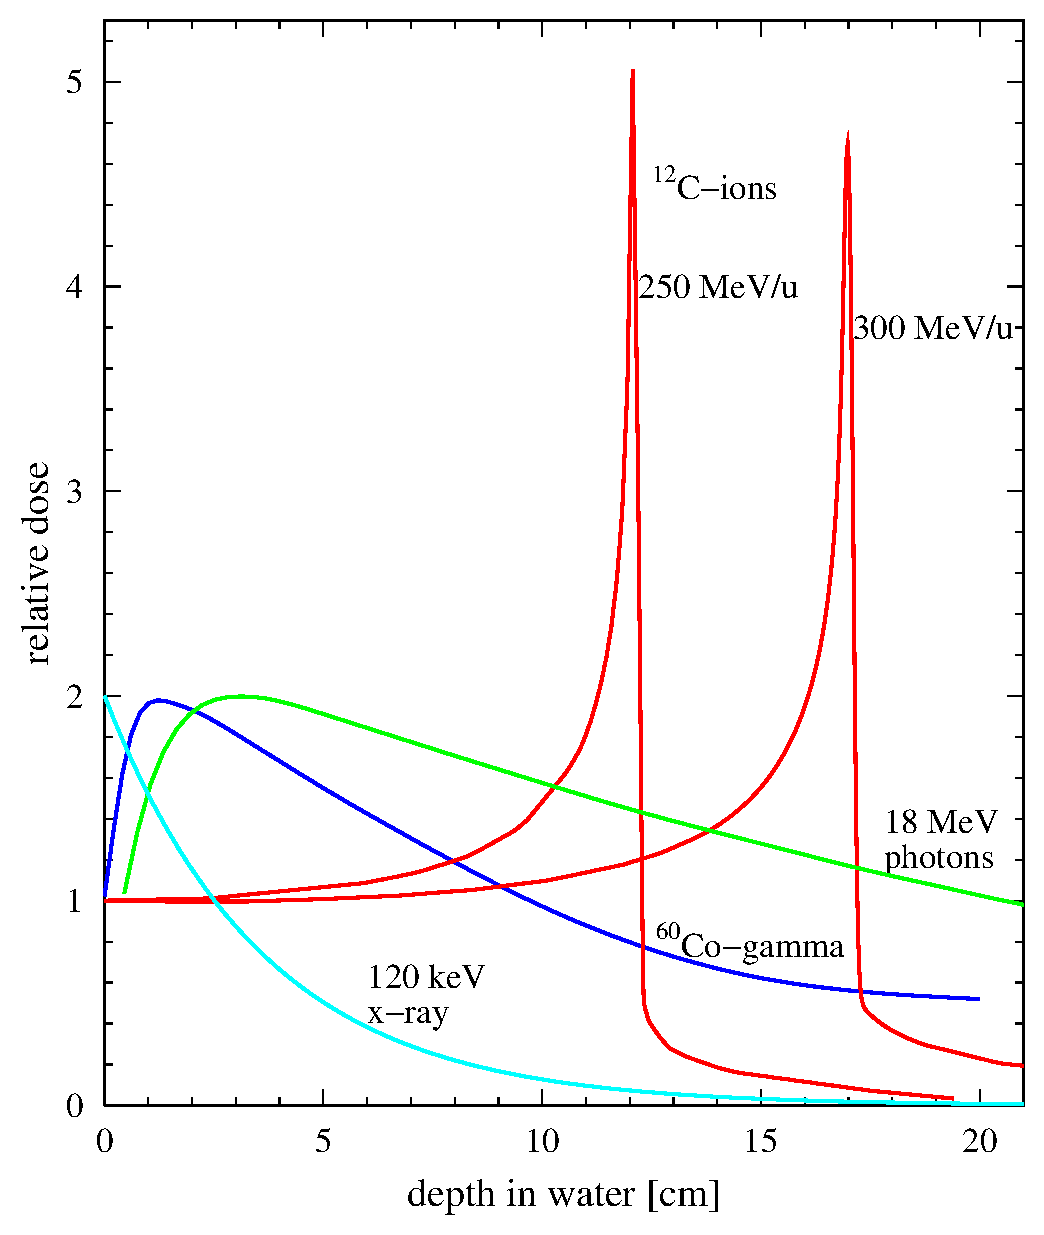
\includegraphics[scale=0.7]{./teile/introduction/depthdose.eps}
\caption{Depth dose distributions of photons and carbon ions at different energies. Photons display an exponential decrease after a certain 
build up. Ions on the other hand interact differently with matter, resulting in an increased dose deposition at the end of the particle 
track, the Bragg peak. Figure taken from \cite{Sch10}}
\label{ddp}
\end{center}
\end{figure}
% \newpage

\newpage

\subsubsection{Interaction of photons with matter}

Photons undergo different processes when passing matter, like coherent scattering or Rayleigh scattering, photoelectric effect, Compton 
scattering and pair production. The probability for each process depends on one hand on the energy of the primary photons as well as on the 
atomic number of the absorbing material, while the strength of these dependencies varies in turn on the different processes \cite{Lil06}. 
The overall decrease of the photon beam intensity when passing a material can be described by the following formula:

\begin{equation}
 I = I_{0} \cdot e^{- N \sigma x} = I_{0} \cdot e^{-\mu x}
 \label{expdecrease}
\end{equation} 

where $I_{0}$ represents the intensity of the incident photon, $x$ the depth of the material in units of length, $N$ the atomic density 
of the material and $\mu$ is the attenuation coefficient. The latter is directly related to the overall cross section $\sigma$, which is a 
measure of the probability of the occurrence of an interaction mechanism. It has contributions from all single interaction processes. 

\begin{equation}
{\sigma} = \sigma_{\mathrm{rayleigh}} + \sigma_{\mathrm{photoelectric}} + Z\sigma_{\mathrm{compton}} + \sigma_{\mathrm{pairproduction}} 
\end{equation}

In the energy range of radiotherapy (between 100 keV and 25 MeV) the dominating process is Compton scattering \cite{Alp98}. 
The attenuation of the photon beam results thus in the following way: 
The Compton electrons are scattered in a strongly forward direction, leading to a build up effect in deeper layers of the material. The 
maximum of the depth-dose profile is reached when the electrons are completely stopped at a certain depth, which is called the mean electron 
range (and is dependent on the initial photon energy). Afterwards the dose deposition decreases exponentially (see eq. \ref{expdecrease}). 


\subsubsection{Interaction of ions with matter}

Interaction of ions with matter occurs via one of the following processes: elastic coloumb scattering from target nuclei (nuclear stopping) 
and inelastic collision with target electrons (electronic stopping). In the mildly relativistic region used in radiotherapy 
(energies of less than 500$\mathrm{MeV}/\mathrm{u}$) the total stopping power of ions is dominated by electronic stopping, 
resulting in ionization and excitation of the target atoms. 
The Bethe-Bloch formula \cite{Bet30, Blo33}, describing the mean rate of energy loss of relativistic ions, can thus be corrected 
for low particle energies \cite{Nak10}, resulting in the following approximation:

\begin{equation}
- \left \langle \frac{dE}{dx} \right \rangle = \frac{ 4 \pi N_{e} z_{eff}^{2} }{ m_{e} v^{2} } \left( \frac{e^{2}}{4\pi \epsilon_{0}} \right) ^{2} \left[ln \left( \frac{2m_{e}v^{2}}{I} \right) + \mathrm{correction} \right]
 \label{bethe}
\end{equation}

where $N_{e}$ is the materials electron density, $e$ and $m_{e}$ are the charge and mass 
of an electron, $\epsilon_{0}$ the electrical field constant and $I$ the mean excitation energy of the absorber material. The effective 
projectile charge $z_{eff}$ can be approximated by the Barkas formula \cite{Bar63}, where $\beta$ is the projectile speed in units of 
$c$: 

\vspace*{-0.8cm}
\begin{equation}
 z_{eff} = z \left( 1 - e^{-125 \beta z^{\frac{2}{3}}} \right)
\end{equation}

The main dependencies of the mean rate of energy loss can be seen in equation \ref{bethe}. It is proportional to $z_{eff}$ 
and inversely proportional to $v^{2}$. The overall depth dose distribution can thus be understood in the following way: in the beginning 
the particles have a high energy and thus high velocity, causing the dose deposition to be small. While passing the material, the velocity 
of the projectile decreases, causing the energy deposition to increase. At low particle energies, close to the particle range, 
target electrons are collected hence causing $z_{eff}$ to decrease, leading to a decrease in dose deposition. The position of the maximum 
specific energy loss around the particle range is known as Bragg peak. 

\subsubsection{Range straggling and lateral scattering}
\label{scat}
Even though electronic stopping via inelastic collisions with target electrons is the main interaction process in the therapeutic energy 
range, elastic Coulomb scattering from target nuclei is still occurring and represents the main reason for lateral scattering. In an analytical 
approximation by Moli\`{e}re \cite{Mol48}, the angular spread of the overall deflection in a material has been described. It is 
on one hand dependent on the mass of the target nuclei, where a higher mass causes a larger angular spread for the same material thickness. 
And on the other hand it is inversely proportional on the momentum of the projectile, causing carbon ions to have a smaller 
lateral deflection than e.g. protons. Experimental validation comparing carbon ions to protons having the same range in water 
(15.6cm, 150MeV protons and 285MeV/u 12C ions) resulted in an approximately three times smaller angular spread \cite{Sch10}.\newline
\newline
Range straggling is caused by the statistical fluctuations of single electronic stopping events. In case of large number of collisions or 
thick layers of material these fluctuations can be approximated by a Gaussian probability distribution \cite{Bor40} 
\cite{Ahl80, Ric12}. This leads to an inverse proportional dependence between the ratio of the straggling width $\sigma_{R}$ with 
the mean range $R$ and the square root of the ion mass $M$ ( $\mathrm{\sigma_{R}}/\mathrm{R} \propto \mathrm{1}/{\sqrt{M}}$ ). This results 
in a smaller range scattering for heavier ions. Experimentally, the ratio between the straggling width and the mean range was found to be 
3.5 smaller for carbon ions compared to protons \cite{Sch10}.


\subsubsection{Nuclear fragmentation}
\label{intro:nt}
At large penetration depths, when the projectile ions have lost most of their energy, projectile fragmentation processes start to be 
relevant for ions heavier than protons. Mostly lower Z fragments are produced, which move with approximately the same velocity 
and in the same direction as the primary ions. This causes dose tails behind the Bragg peak position (see figure \ref{int:frag:fig}). 
Thus the resulting depth-dose distribution is actually the sum of the energy deposition of the projectiles and the resulting 
fragments. 

\begin{figure}[H]
\begin{center}
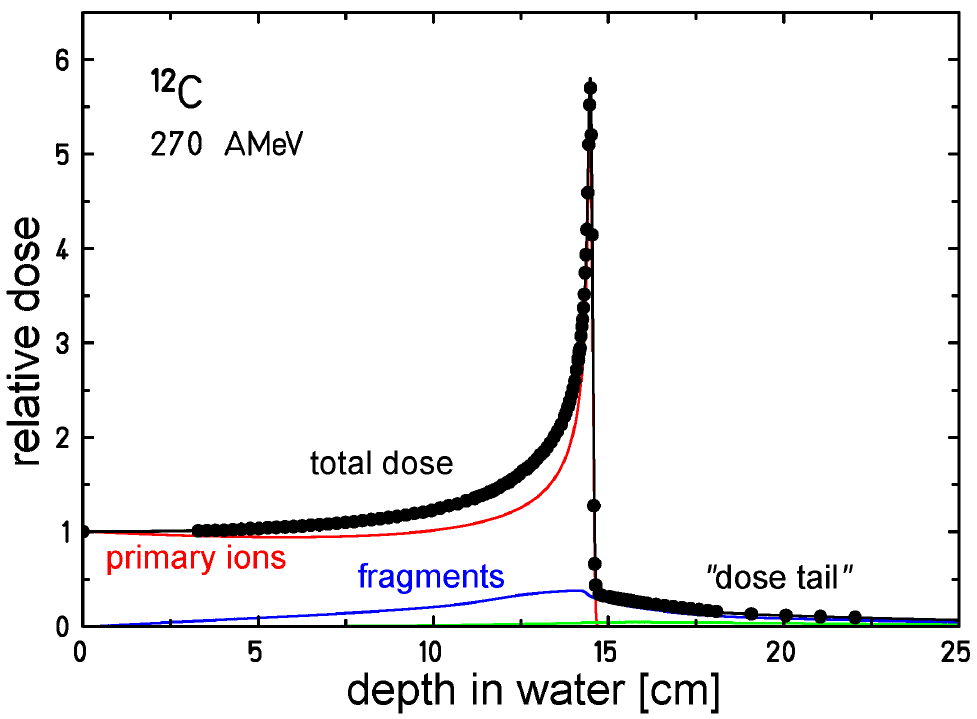
\includegraphics[scale=0.3]{./teile/introduction/iondepthdosesum.png}
\caption{Depth dose distribution of carbon ions. Besides of the energy deposition of the primary ions (red), the produced fragments 
(blue curve) contribute to the overall dose deposition (black) and are especially visible in the dose tail behind the Bragg 
peak. Figure taken from \cite{Gro04}}
\label{int:frag:fig}
\end{center}
\end{figure}

Nevertheless, the produced fragments  also offer the chance for PET (Positron Emission Tomography) monitoring, 
without additional radiation exposure for the patient. As peripheral collisions are more frequent then central ones \cite{Kra00} 
isotopes like $^{11}C$ and $^{10}C$ are often produced when $^{12}C$ ions penetrate through tissue. Both isotopes are $\beta^{+}$ 
emitters. They annihilate with electrons in the human body, producing two $\gamma$-rays which travel in opposite directions.

% \newpage

\subsubsection{Track structure}

For inelastic collisions with atomic target electrons, only about 20\% of the initial projectile energy is used to overcome the 
electron binding energy \cite{Kra92}. A high amount of energy is transformed into the kinetic energy of the secondary electrons, the 
so-called $\delta$-electrons. These $\delta$-electrons can in turn emerge from the primary particle trajectory and undergo frequent 
elastic and inelastic scattering. If their energy is sufficiently high they can induce further ionization in more distant locations, 
leading to a high number of additional electrons. The radial dose fall off is approximated by a $\mathrm{1}/\mathrm{r^{2}}$ law, 
illustrating that the radial dose quickly falls off with larger radial distance $r$ \cite{Cha76, Kat99, Ric12}. 
The range of the $\delta$-electrons is restricted to a maximum value according to the kinematics of the collision between projectile 
and target electron. Empirically this can be described by a power law \cite{Kie86}, where $E$ is energy of the primary ion:

\begin{equation}
 r_{max} \propto E^{1.7}
\end{equation}

As stated by the Bethe equation (\ref{bethe}), the energy deposition of the primary ions is dependent on the used ion species and their 
energy. This results in a higher stopping power for higher $Z$ primary ions as well as an increased stopping power for smaller energies. 
Hence carbon ions have a much higher $\delta$-electron output than e.g. protons. Furthermore with decreasing energy of 
carbon ions, the $\delta$-electron output increases. This can be seen in figure \ref{track}. The higher ionization density produced by 
$\delta$-electrons is also the reason for the difference in induced biological damage. 

\subsubsection{Linear Energy Transfer LET}


The critical measure for the energy deposition of the $\delta$-electrons is the linear energy transfer (LET). 
It is defined as the locally deposited energy to the medium (average energy deposited per unit length of track \cite{Hal06}) and 
in radiobiology is given in keV/$\mu$m. Sparsely ionizing radition (such as photons, protons and fast ions) have a low LET, while slow ions 
are densely ionizing and hence have a high LET. 


\newpage

\vspace*{1cm}

\begin{figure}[H]
\begin{center}
% 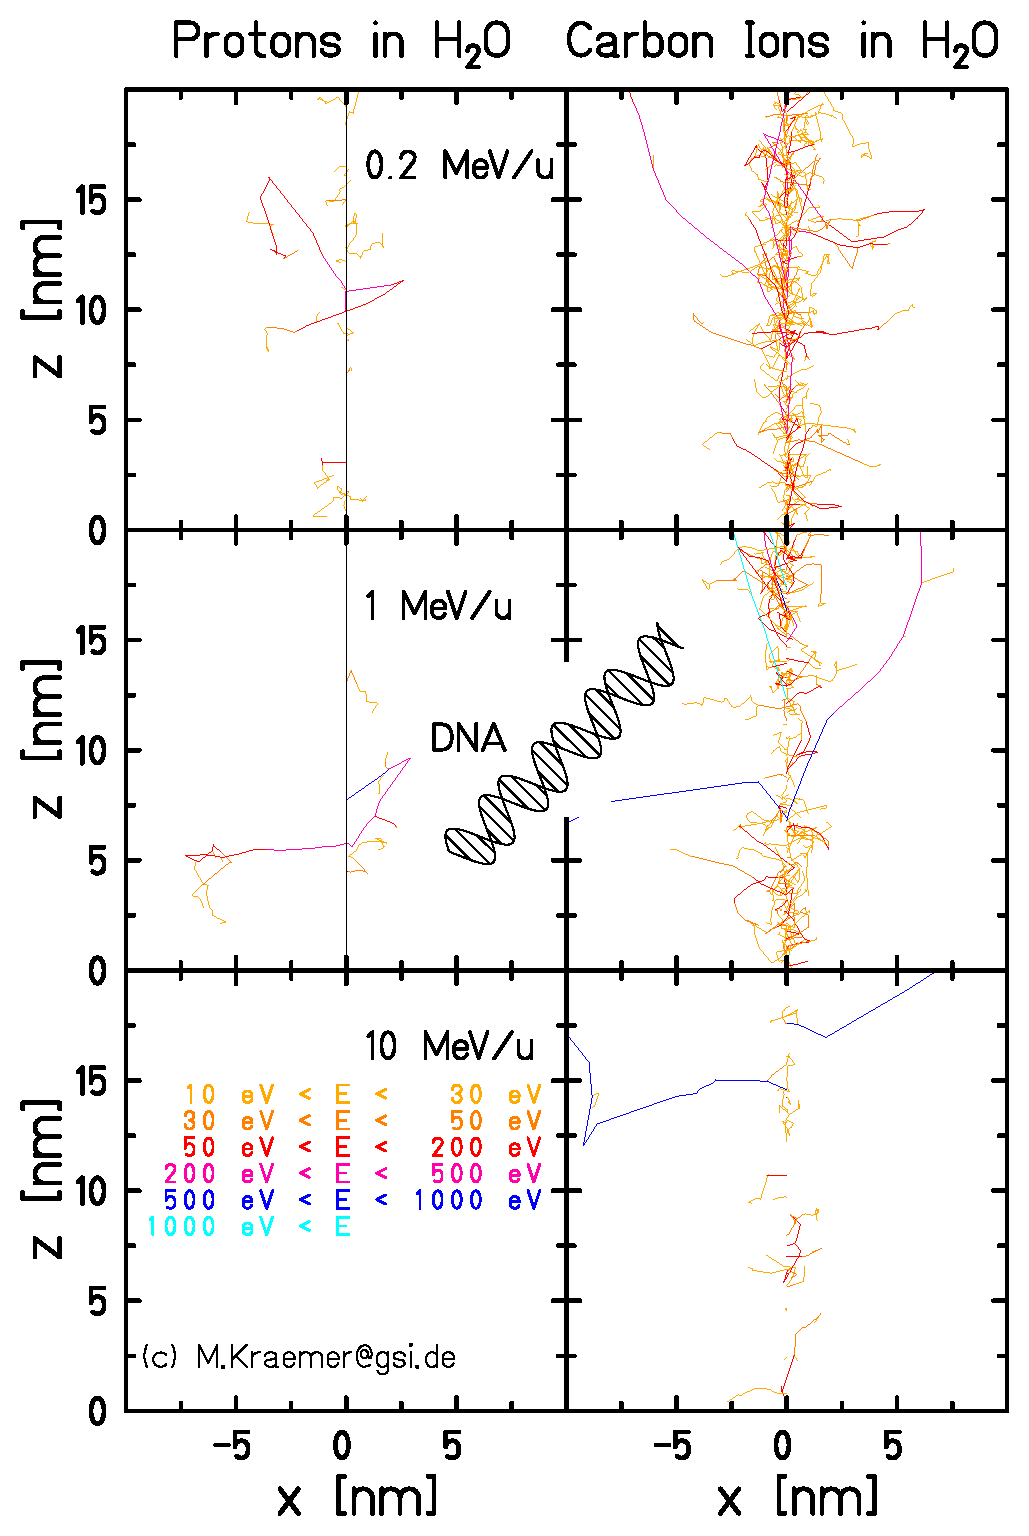
\includegraphics[scale=0.75]{trackstructure.eps}
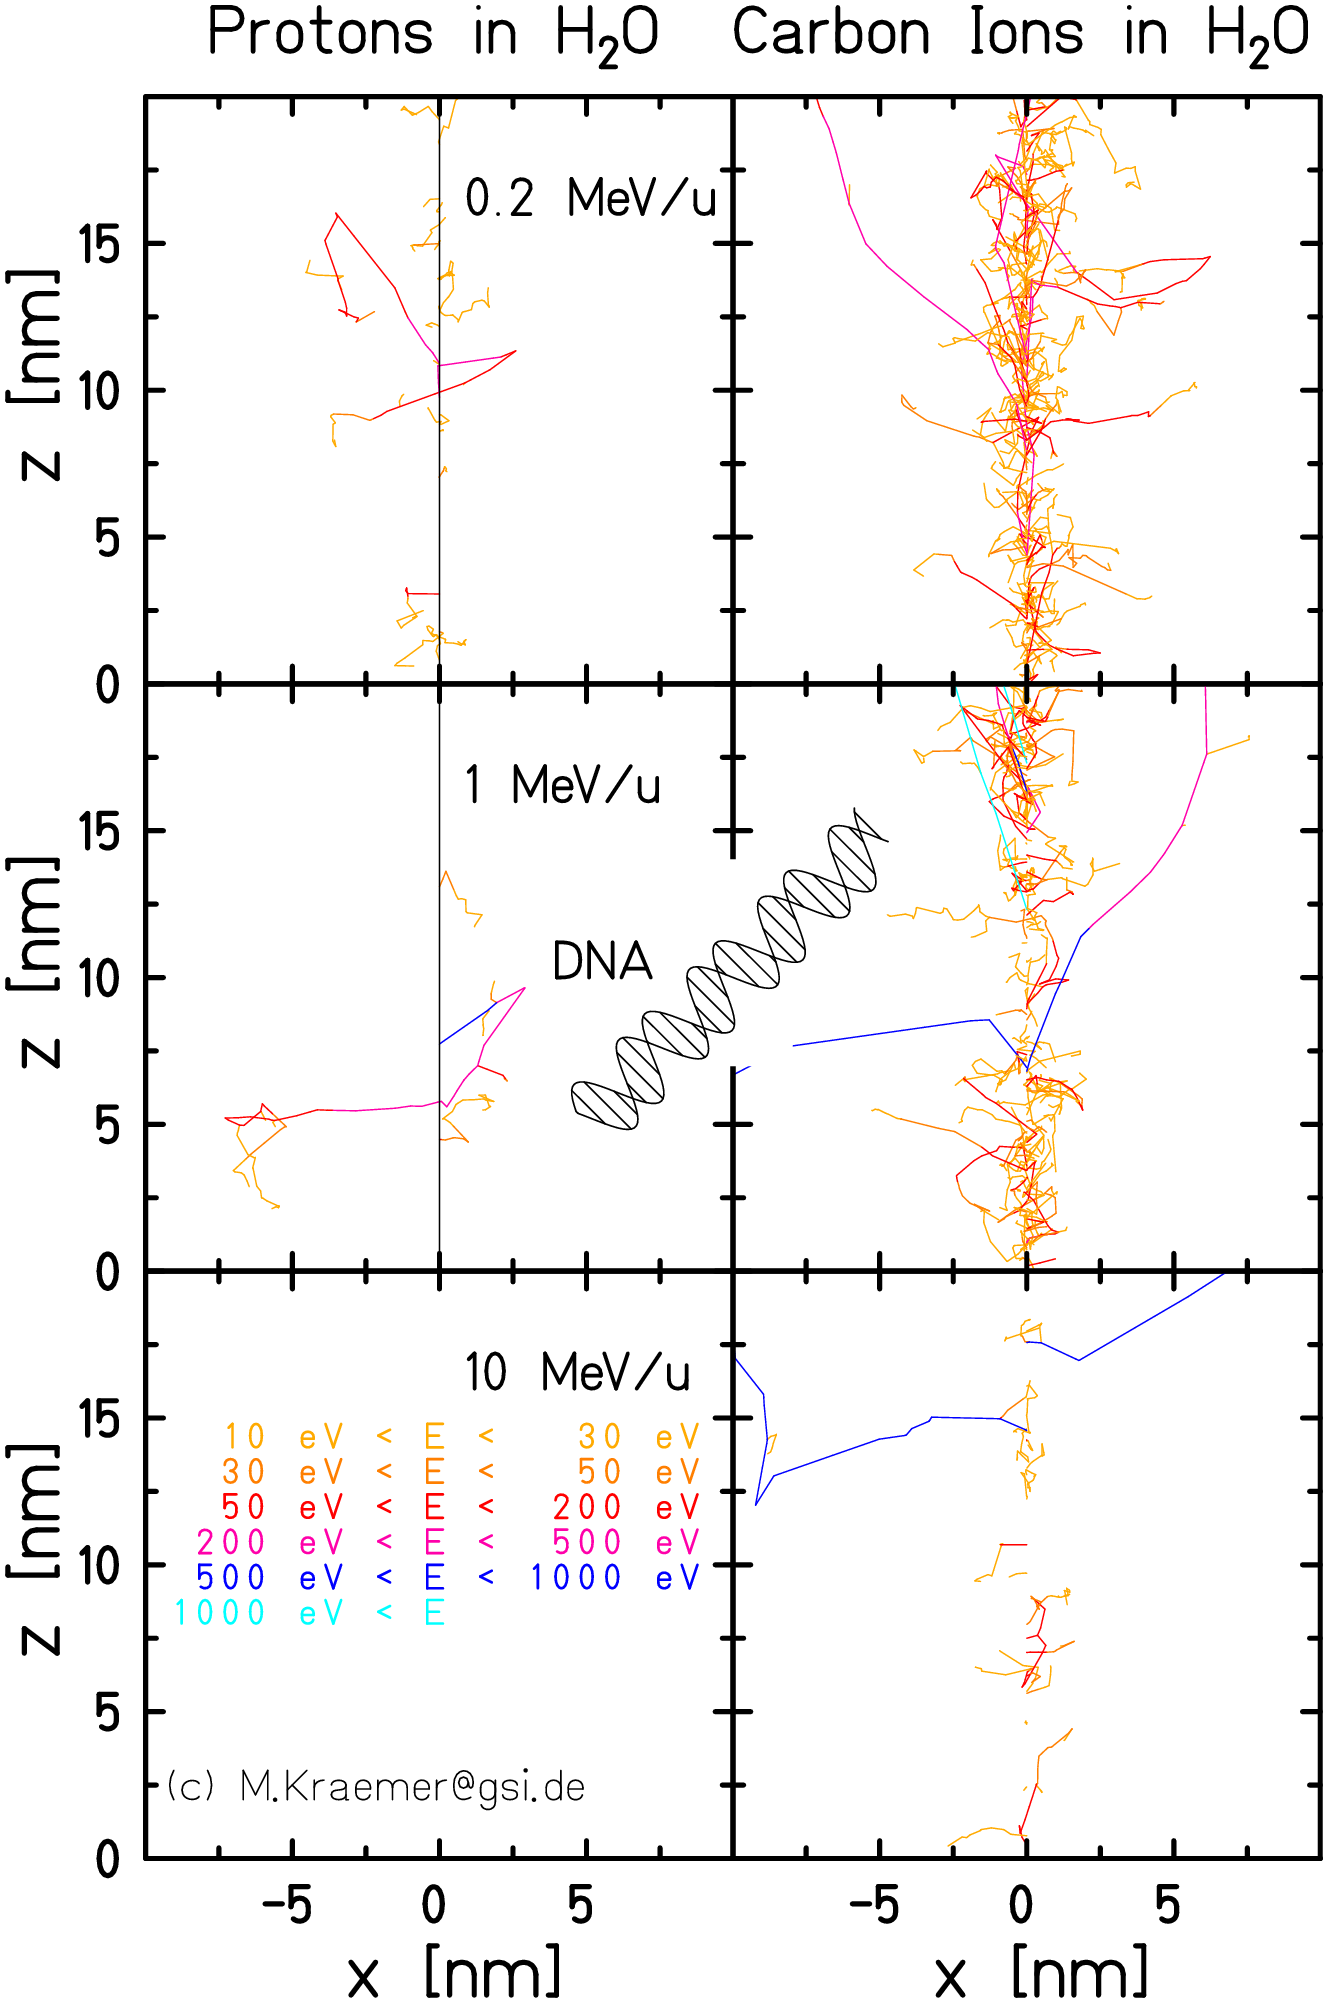
\includegraphics[scale=0.25]{./teile/introduction/trackstructure.png}
\caption{Microscopic track structure of protons (left side) and carbon ions (right side) at different energies. Protons and high energy 
carbon ions are low LET radiation and hence sparsely ionizing. Low energy carbon ions on the other hand are high LET radiation and hence 
densely ionizing. For comparison the size of the DNA is displayed. Figure courtesy of Michael Kr\"amer.}
\label{track}
\end{center}
\end{figure}



\subsection{Radiobiology}
\label{radiobio}
It was described in the previous section that both, photons and ions, are ionizing radiation producing $\delta$-electrons which 
in turn can cause subsequent ionizations. These ionizations attack the carrier of the genetic information, the DNA, of the irradiated 
cells and hence causes them to stop to proliferate. The biological background of these processes will be described in this section. 
Furthermore the enhanced biological effect of ions compared to photons will be explained. This is one of the potential benefits expected 
from a non-invasive irradiation of atrial fibrillation with carbon ions compared to photons. 


\subsubsection{Impact of radiation on cells}

In eukaryotic cells, meaning cells that contain a cell nucleus, the genetic information is stored in the DNA (desoxyribonucleic acid), 
making it therefore the critical target in radiotherapy. DNA is made of two sugar and phosphate backbones and four different base pairs 
(adenine A, cytosine C, guanine G and thymine T), which bind in a defined way (A with T and C with G) and thus form the double helix 
structure with a distance between the two strands of about 2 nm. The genetic information is encoded in the sequence of the base pairs. 
Ionizing radiation can destroy the described structure of the DNA, either by direct or indirect action \cite{Hal06}.\newline
\newline
As can be seen in figure \ref{ida} direct effects are caused by the destruction of molecular bonds of the DNA itself 
through any form of radiation. This process is considered the dominant effect if radiation with a high LET is used. Indirect action means 
that free radicals are produced by the ionizing radiation, which then in turn can damage the DNA. 
This phenomenon is predominant when sparsely ionizing radiation (low LET, like photons) are used and interact with molecules in the cell, 
particularly water.\newline
\newline
Both mechanisms can cause either single strand breaks (SBS) or double strand breaks (DSB) (see figure \label{ida}). SSB means that only 
one of the strands is destroyed, leaving the complementary base on the other strand intact and thus enabling a fast repair if the SSBs 
occur at a certain distance from each other. DSBs or clustered SSBs are more complex and can cause the breakage of the chromatin. But even 
these damages are usually steadily repaired. The repair mechanisms only start to fail when the DSBs accumulate to local lesions. Changes 
in the original DNA material is the result. Depending on the produced damage mutations, carcinogenesis or cell death can be the 
result. Cell death can occur in different pathways. Apoptosis is the controlled self-inactivation of the cell due to DNA damage and the preferred 
pathway in radiotherapy. Uncontrolled cell death, necrosis, typically causes severe reactions of the immune system, leading to e.g. 
inflammation.

\begin{figure}[H]
\begin{center}
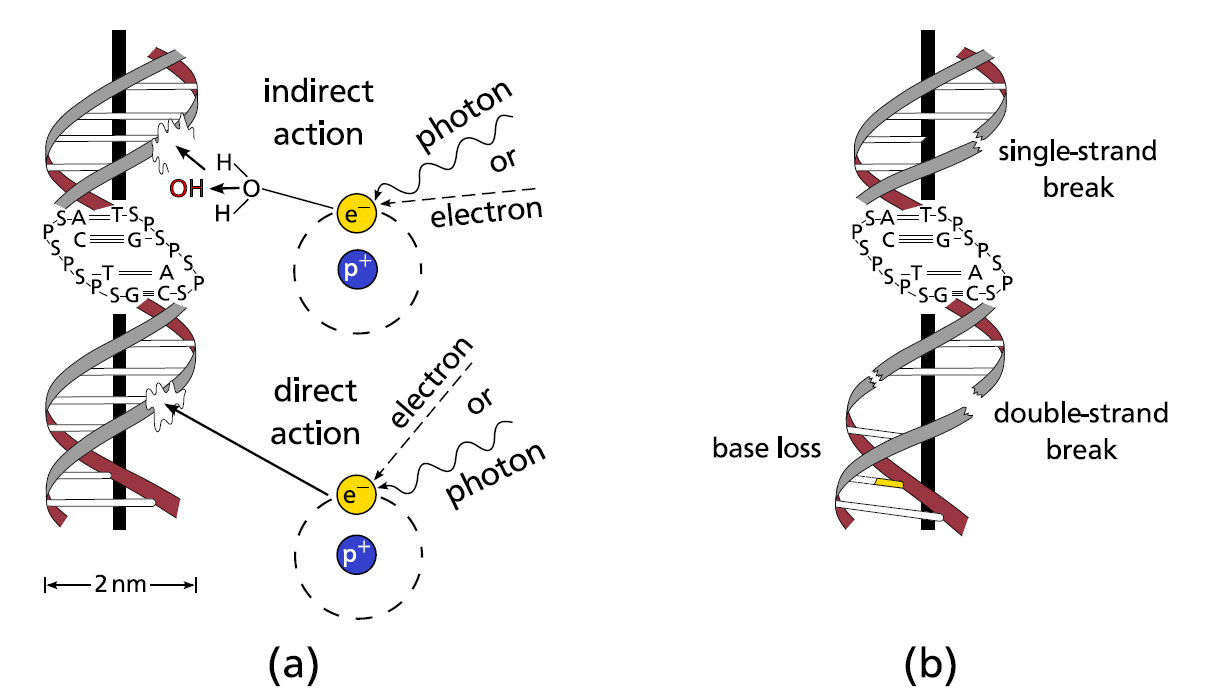
\includegraphics[scale=0.5]{./teile/introduction/SSB_DSB.png}
\caption{On the left side (a) direct and indirect radiation damages are illustrated. On the right side (b) single strand breaks and 
double strand breaks are visualized. Figure taken from \cite{Ric12}}
\end{center}
\label{ida}
\end{figure}



\subsubsection{Relative Biological Effectiveness RBE}

As outlined, at the same dose level radiation the damage depends on the LET.  This means that the induced biological effect 
is, amongst others, dependent on the energy and type of radiation. This is described in the relative biological effectiveness (RBE), 
which is defined as follows:

\begin{equation}
 RBE = \left.\frac{D^{ref}_{photon}}{D_{ion}} \right|_{\mathrm{isoeffect}}
\end{equation}

$D^{ref}_{photon}$ is the absorbed photon dose necessary to induce a certain isoeffect and $D_{ion}$ is the absorbed dose of ions at a 
defined energy which leads to the same effect. Comparison of RBE values are valid only for the same effect and biological endpoint 
and by using the same reference radiation. This idea is used in the local effect model (LEM) at GSI for the prediction of the RBE. By 
assuming that the biological effect is independent of the specific radiation type but rather dependent on the energy deposition distribution 
in small sub volumes of the cell nucleus, RBE predictions are computed in relation to the known biological response of photons 
\cite{Krae03, Fried13}. Weighting the physically absorbed dose with the RBE results in the biological dose in units of Gray equivalent 
(GyE). \newline
\newline
The RBE depends on multiple parameters, like the endpoint, the irradiated tissue and its repair mechanism, the particle type, 
the used dose level and the LET. The dependence between RBE and LET is illustrated in figure \ref{rbe_let}. In case of x-rays (sparsely ionizing) 
the probability of an induced DSB is low and in general more than one track would be required to induce DSBs, resulting in a small RBE. 
Irradiation with a LET around 100keV/${\mu}$m on the other hand is optimal in producing a biological effect, as the 
density of ionization coincides with the diameter of the DNA double helix of about 2nm. Thus radiation with this LET has the 
highest probability to induce a biological damage with DSBs. More densely ionizing radiation (LET > 200keV/${\mu}$m) produces many DSBs, 
leading to ionization events which are closer together than needed. The RBE consequently decreases again, an 
effect known as overkill effect. 

\begin{figure}[H]
\begin{center}
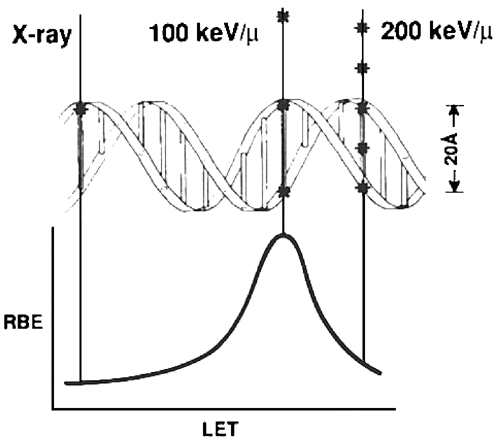
\includegraphics[scale=0.5]{./teile/introduction/rbe_let.png}
\caption{Photon radiation with a LET of 100 keV/${\mu}$m has the biggest RBE for cell killing due to the fact that average separation between 
ionizing events coincides with the diameter of the DNA double helix (2 nm). Figure taken from \cite{Hal06}}
\label{rbe_let}
\end{center}
\end{figure}

Concerning the increased biological effectiveness of ions it can be stated that it is only of advantage if the RBE is more pronounced 
in the target tissue compared to the normal tissue in the entrance channel. While protons exhibit an almost constant RBE throughout the 
energy deposition (a constant value of RBE = 1.1 is used), for ions heavier than oxygen the location for the highest RBE moves towards the 
proximal region of the depth-dose profile, starting to coincide with the plateau region \cite{Kra00}. For carbon ions on the other hand 
the position of the highest RBE value coincides with the Bragg peak region, enhancing the possibility of a beneficial treatment outcome. 



\newpage

%%%%%%%%%%%%%%%%%%%%%%%%%%%%%%%%%%%%%%%%%%%%%%%%%%%%%%%%%%%%%%%%%%%%%%%%%%%%%%%%%%%%

\section{Radiotherapy}

The conventional method for radiotherapy remains the irradiation with photons. Nevertheless, the biological and physical properties of ions 
(which were described in the previous section) result in advantages for radiotherapy, especially when treating deep seated targets. 
As a result, more and more ion facilities are opened worldwide, treating an increasing number of patients with protons and carbon ions \cite{Loe13}. 
In this section the state of the art in treating static tumors with photon and carbon ion therapy will be summarized. 
Afterwards organ motion and the resultant difficulties, as well as approaches for motion mitigation will be presented. 

\subsection{Photon therapy}

As can be seen in figure \ref{ddp}, a treatment of deep seated targets with photons can be carried out more effectively the higher the photon 
energy. Over the decades, different photon emission techniques were developed which allowed for higher photon energies. 
Currently, photons in the energy range of (6-25)MeV \cite{Ber06} are used. The photons are produced with the help of linear accelerators, which 
are used to shoot accelerated electrons on a target, thereby emitting bremsstrahlung which is then used for radiotherapy.\newline
\newline
Not only the used photon energy spectrum but also the application techniques developed over the last decades \cite{Buc05}. Two dimensional (\textbf{2D}) 
radiotherapy was based on radiographies and was carried out with a single beam, which was applied from one to four different directions, 
usually as opposing lateral fields. As the imaging techniques advanced the treatment became also more conformal. CT scans enabled axial anatomy 
and tumor visualization in three dimensions. Hence in three dimensional conformal radiotherapy (\textbf{3DCRT}) more accurate dose calculations 
with homogeneous fields are possible, leading to an increased normal tissue sparing. With the development of \textbf{IMRT} (intensity 
modulated radiotherapy) the normal tissue sparing could be further improved. In IMRT a varying number of beams 
from different beam directions are overlaid while modulating the intensity of radiation within each field. This intensity modulation is 
achieved by using multileaf collimators (MLC) (see figure \ref{lamellen}). An exemplary IMRT treatment plan in comparison to carbon ion 
irradiation can be seen in figure \ref{targetvergleich}. 

\vspace*{-0.3cm}

\begin{figure}[H]
\begin{center}
% \includegraphics[scale=0.28]{lamellen.png}
\includegraphics[scale=0.2]{./teile/introduction/lamellen.png}
\caption{Technical realization of IMRT by using multileaf collimators (MLC), enabling a photon dose deposition conformal to the 
target volume. Each lamellae can be moved individually, enabling an intensity modulation. Figure taken from \cite{Schl01}}
\label{lamellen}
\end{center}
\end{figure}


\subsection{Carbon therapy}

As already explained in section \ref{pbb} ions display an inverse depth-dose profile and a higher biological effect compared to photons. 
This enables a high target conformity and a sparing of normal tissue, both of which are beneficial for radiotherapy. 
Since 1954, when the first ion beam therapy was carried out with protons at Berkeley Lab \cite{Tob58} different projectile ions were 
used and their effect on target tissue studied.\newline
\newline
Due to the their higher momentum and thus smaller lateral scattering (see section \ref{scat}) the usage of heavy ions (heavier than protons) 
enables a better sparing of normal tissue and organs at risk (OAR), even if they are close to the target volume. 
In contrast to other ion types, the increased biological effectiveness of carbon ions  coincides with the Bragg peak region (see section 
\ref{radiobio}). Thus both the physical and biological properties of carbon ions offer the possibility of a beneficial treatment outcome. 

\subsubsection*{Application technique}

As in photon therapy, ion therapy application and thus target conformity improved over the decades after first treatments at Berkeley 
were performed by shooting the proton beam through the complete patient head \cite{Tob58}. Depending on the provided accelerator as well 
as on the beam line properties passive and active techniques are distinguished both in beam delivery as well as beam shaping.\newline
\newline
Concerning \textbf{beam delivery} particle acceleration to the therapeutic energies of several hundred MeV/u is carried out in cyclotrons and 
synchrotrons. \textbf{Cyclotrons}, which are used mainly in proton centers, offer the advantage of a more compact design compared to synchrotrons 
and allow a continuous beam extraction with stable intensities. On the other hand no active energy variation is possible, requiring the need 
for passive energy degraders. \textbf{Synchrotrons}, which are used in heavy ion centers, allow active energy variation.\newline
\newline
Concerning \textbf{beam shaping} methods, which are used in order to deposit a homogeneous dose in the target volume, \textbf{passive methods} 
are used in some carbon ion centers as well as in the majority of proton centers. The devices rely on three different beam shaping steps 
\cite{Chu93}. Firstly the beam is broadened by scattering and then further widened by using range modulators like e.g. a 
ridge filter. Thereby an extended and flat, but still homogeneous, field is formed which covers the tumor extent in longitudinal direction 
(Spread Out Bragg Peak: SOBP). Secondly, the range adjustment of the SOBP is achieved via flat degraders of variable thickness. Final 
conformity to the distal target border is achieved by patient individual compensators. Collimators are used for a lateral 
conformity. A scheme of a passive beam shaping system can be seen in figure \ref{passive}. Passive beam shaping devices offer the benefit 
that the historically unstable beam quality of research facilities - in which the first treatments were carried out - did not influence the 
homogeneity of the applied dose. Moreover, beam energy changes during treatment can be avoided, thus enabling a fast irradiation time. 
Nevertheless, passive beam application always requires the manufacture of patient individual compensators and an unavoidable limitation in 
volume conformity in the proximal tumor region as the SOBP width is fixed by the range modulator to the largest needed depth (see 
figure \ref{passive}). Material in the beam path means furthermore intensity loss due to lateral scattering and an extra dose exposure 
due to fragmentation.


\vspace*{0.8cm}
\begin{figure}[H]
\begin{center}
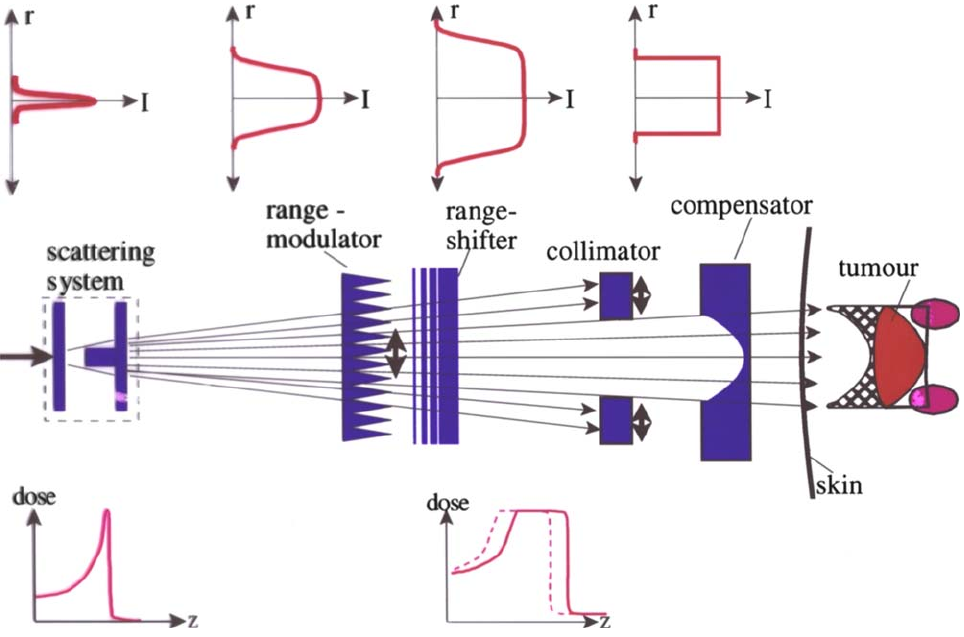
\includegraphics[scale=0.4]{./teile/introduction/deliverypassive.png}
\caption{Scheme of a passive beam shaping system. The beam is broadened by a scattering system and the width of the SOBP is determined by a 
range modulator. Via a range shifter the SOBP energy can be adjusted to a fixed range and thus depth. For lateral conformity collimators are 
used. The longitudinal conformity to the distal border of the target is achieved with a patient specific compensator. The proximal volume 
border can not be shaped, as is indicated in the hatched areas. Figure taken from \cite{Sch10}}
\label{passive}
\end{center}
\end{figure}

\newpage

\textbf{Active beam shaping} is achieved with beam scanning, which offers a very good lateral target coverage as well as volume conformity 
also in the proximal field region. The target volume is thereby subdivided into slices of the same beam energy, so called iso-energy slices 
(IES). Each IES is again subdivided into a grid of target points which are irradiated sequentially. Hence many small pencil beams are used to 
generate a conformal dose deposition to any arbitrary target volume shape without the need of patient specific hardware. This drastically 
decreases the amount of material the beam has to traverse and hence reduces the unwanted neutron dose to the patient \cite{Kad12}. Examples of 
beam scanning are spot scanning, which was developed for protons at the Paul Scherrer Institute (PSI, Swiss) \cite{Ped95} or raster scanning, 
which was developed in parallel at GSI \cite{Hab93}. \newline
\newline
At PSI a cyclotron is used and the energy variation is carried out with a degrader. The lateral deflection of the beam position is either 
achieved with magnets (Gantry 2 at PSI \cite{Ped04}) or a combination of magnets and patient couch motion (Gantry 1). The beam is thereby 
switched off between different beam positions in the order of milli seconds. \newline
\newline
Raster scanning on the other hand works in a continuous irradiation mode for one IES. A pencil beam is extracted from the synchrotron with a fixed energy and thus range, 
corresponding to a IES of the volume. By overlaying many different energies a SOBP is created to cover the longitudinal extension of the tumor 
(see figure \ref{active}b). The raster points within each IES are irradiated by deflecting the pencil beam via two orthogonal dipol magnets 
on an optimized path (see figure \ref{scanning}). When the pre-defined intensity of the raster point has been reached, the beam is moved to the next position. 
In order to establish a homogeneous dose coverage in the target volume the spacing, both in raster point position as well as IES distance, 
can be utilized. Robustness in longitudinal direction can be achieved with overlap of the individual IES slices. Nevertheless the number of 
IES slices should be kept small in order to guarantee a short treatment time. Hence a broadening of the Bragg Peak position is carried out 
with a so-called ripple filter (see figure \ref{active}b). It was found that a spacing of 3mm between IESs yields a robust result \cite{Web99}. 
Furthermore the lateral overlap of the pencil beams needs to be chosen in such a way that the possibility of minor fluctuation in beam 
quality and position is compensated for. As the lateral beam profile is assumed to be Gaussian shaped and symmetric it was found that the 
full width half maximum (FWHM) of the beam is optimally chosen to be three times the raster spacing (see figure \ref{active}a) \cite{Hab93}. 

\newpage

\vspace*{0.6cm}

\begin{figure}[H]
\begin{center}
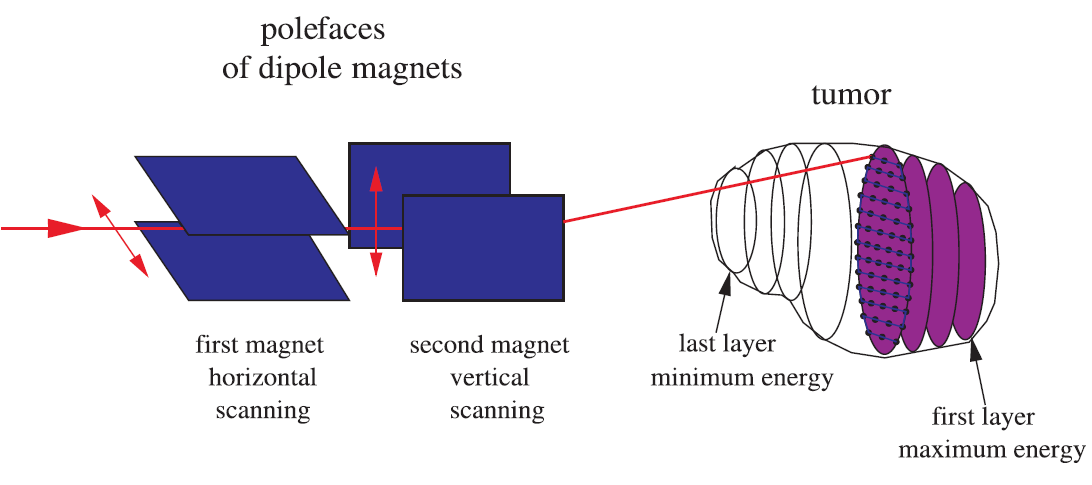
\includegraphics[scale=0.4]{./teile/introduction/therapy.png}
\caption{Principle of the raster scanning technique at GSI. The target volume is divided into IES, which is again subdivided into a regular 
grid. By varying the particle energy from the accelerator and by deflecting the pencil beam via a magnetic scanning system the raster points 
are scanned. Figure taken from \cite{Inf05}}
\label{scanning}
\end{center}
\end{figure}


\begin{figure}[H]
\begin{center}
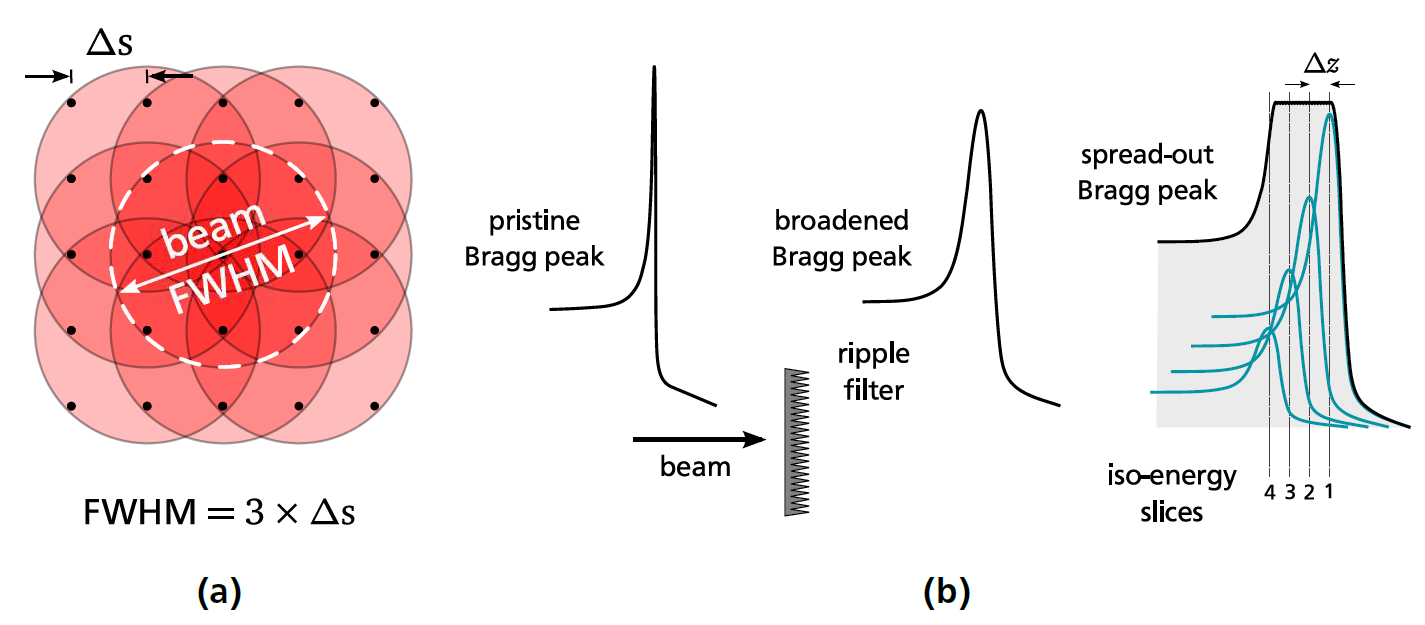
\includegraphics[scale=0.45]{./teile/introduction/active.png}
\caption{Target dose homogeneity is achieved by sufficient overlap in lateral and longitudinal directio. a) In lateral direction the FWHM of 
the pencil beam is adjusted to three times the raster spacing $\Delta\mathrm{s}$. b) In longitudinal direction the Bragg peaks are broadend 
in depth by using a ripple filter and then stacked in depth to a SOBP. An IES spacing $\Delta\mathrm{z}$ of typically 3mm is chosen. 
Figure taken from \cite{Ric12}}
\label{active}
\end{center}
\end{figure}


\newpage

\subsubsection*{GSI pilot project}

Between 1997 and 2008 440 patients were treated with scanned carbon ions at GSI. Mostly head and neck tumors were irradiated. 
The typical fractionation scheme was 20 fractions within three weeks \cite{Schu07}. An example of a resulting 
dose distribution with scanned carbon ions in comparison to IMRT can be seen in figure \ref{targetvergleich}. 
The treatment outcome for skull-based chordomas can be seen in figure \ref{chordoma}. In a later stage, also prostate and spinal cord 
tumors were treated.

\begin{figure}[H]
\begin{center}
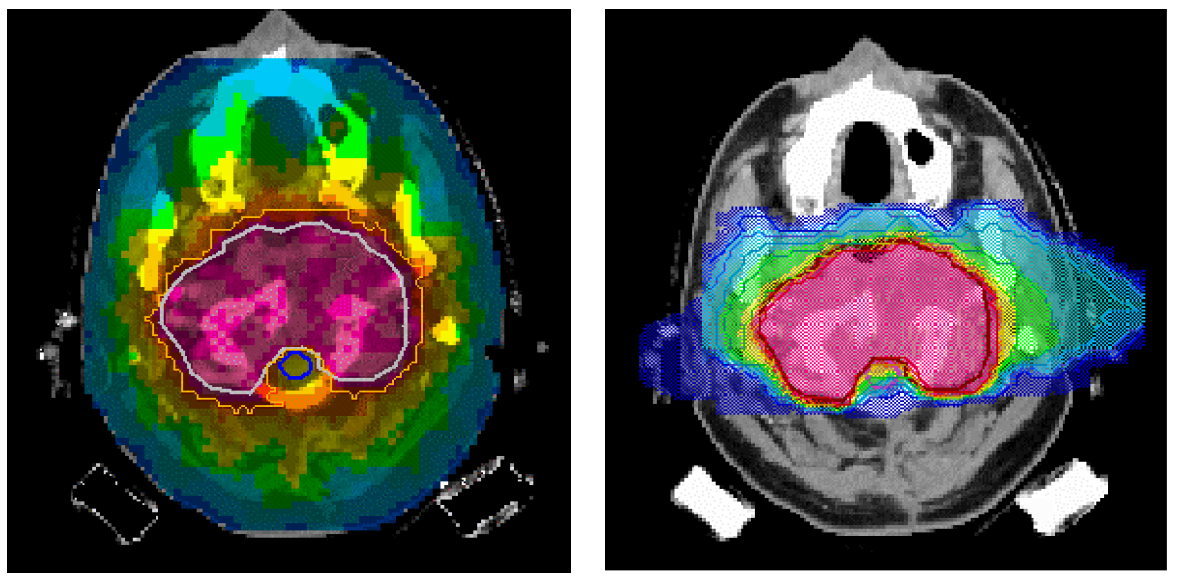
\includegraphics[scale=0.25]{./teile/introduction/targetvergleich.png}
\caption{Comparison of dose distributions results with IMRT (left side) and scanned carbon ions (right side). The dose to the normal 
tissue and especially organs at risk like the brainstem are drastically reduced for scanned carbon ions. Figure taken from \cite{Gro04}}
\label{targetvergleich}
\end{center}
\end{figure}

\vspace*{-1cm}

\begin{figure}[H]
\begin{center}
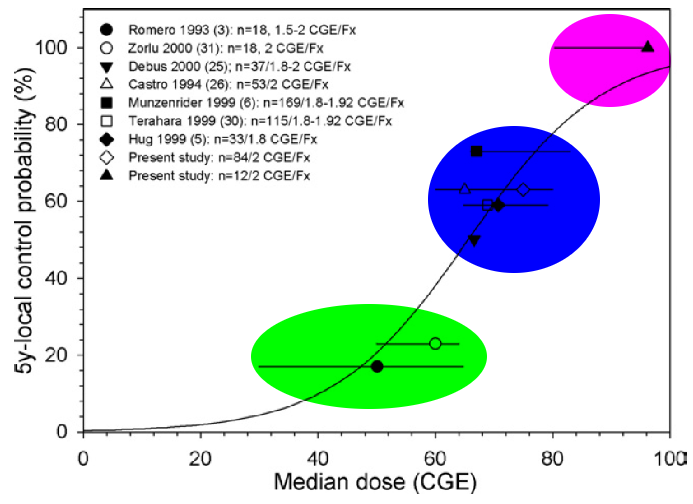
\includegraphics[scale=0.35]{./teile/introduction/chordoma_farben.png}
\caption{Treatment outcome for the irradiation of skull-based chordomas for photons (green area), protons (blue area) and carbon ions (pink 
area). An improved effect after the irradiation of chordomas can be seen when doses exceeding 70 Cobalt Gray Equivalent (CGE) can 
be applied. For carbon ions ahigher dose can be deposited in the target since the dose in the nearby OAR can be reduced. Figure taken 
from \cite{Schu07}}
\label{chordoma}
\end{center}
\end{figure}

The pilot project at GSI was carried out in a collaboration between GSI, the Heidelberg University hospital, the German cancer research 
center (DKFZ) and the research center Dresden-Rossendorf. Following the success in treatment outcome \cite{Loe13} the Heidelberg Ion-Beam Therapy 
Center (HIT) was build, where patients are treated with scanned carbon ion beams and protons on a regular basis since 2009 \cite{Com10}. 
Furthermore CNAO (centro nazionale di adroterapia oncologica, Pavia, Italy) \cite{Ama04} started treating patients with scanned carbon ions 
beams in 2012 \cite{PTCOG13}. In total roughly 10,000 patients have been treated with carbon ions up to the beginning of 2013 \cite{Loe13}, 
whereof about 2,000 patients were treated with scanned carbon ions \cite{PTCOG13}.


\subsection{Treatment planning}
\label{tp}
Treatment planning is the optimization process in which the needed machine delivery parameters are determined for a chosen beam 
configuration in order to yield the prescribed dose to the target volume, while minimising the dose to the normal tissue, ecspecially 
to the OARs \cite{Ric12}. In modern radiotherapy treatment planning is based on CT scans, which represent photon attenuation through 
the different tissue types (Hounsfield units - HU) and can hence be converted to water-equivalent depths. On the patient image data the 
target and OARs are contured and the needed dose and dose constraints, respectively, are determined. For cancer radiotherapy the delineation 
of the tumor includes certain safety margins, defined by the International Commission on Radiation units and Measurements (ICRU). As some 
of these margins will be also used in the context of cardiac targets, they will be shortly introduced here. 

\begin{enumerate}
 \item [] \textbf{GTV (Gross Tumor Volume)}: "The GTV is the gross palpable or visible/demonstrable extent and location of the malignant 
 growth." \cite{ICRU93a}
 \item [] \textbf{CTV (Clinical Target Volume):} "The CTV is a tissue volume that contains a GTV and/or subclinical microscopic malignant 
 disease, which has to be eliminated. This volume thus has to be treated adequately in order to achieve the aim of therapy: cure or 
 palliation." \cite{ICRU93a}
 \item[] \textbf{PTV (Planning Target Volume):} "The PTV is a geometrical concept, and it is defined to select and appropiate beam size 
 and beam arrangements, taking into consideration the net effect of all the possible geometrical variations, in order to ensure that the 
 prescribed dose is actually absorbed in the CTV." \cite{ICRU93a}
 \item[] \textbf{IM (Internal Margin):} "The IM, commonly asymmetric around the CTV, is intended to compensate for all movements and all 
 variations in site, size and shape of the organs and tissues contained or adjacent to the CTV. They may result e.g. from respiration, 
 different fillings of the bladder, different fillings of the rectum, swallowing, heart beat, movements of the bowel" \cite{ICRU99}
\end{enumerate}

Based on this definition, the \textbf{ITV (Internal Target Volume)} is commonly used for the volume in which the IM encompasses the CTV 
(see figure \ref{int:margins:fig}). 

\begin{figure}[H]
\begin{center}
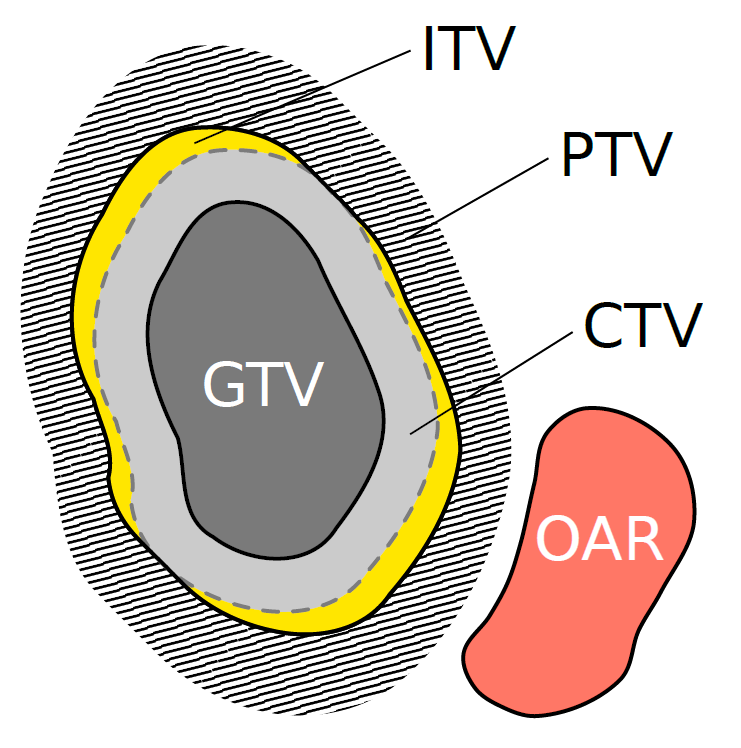
\includegraphics[scale=0.3]{./teile/introduction/volumes.png}
\caption{Treatment planning volumes as defined by the ICRU. Figure taken from \cite{Ric12}}
\label{int:margins:fig}
\end{center}
\end{figure}

\vspace*{-0.3cm}

As a result of treatment planning the ICRU recommends that 100\% of the PTV should receive at least 95\% and not more than 107\% of the 
prescribed dose \cite{ICRU93a}. In order to study if this recommendations are met, dose-volume-histograms (DVH) are computed in the 
treatment planning study process and the values V95 and V107 (the volume which receives 95\% and 107\% of the dose, respectively) determined. 
Furthermore D5 and D95, which denotes the dose covering 5\% and 95\% of the volume, are extracted. The difference between these two values 
(D5-D95) is a measure for the dose fall off and should be ideally close to zero. In general, the dose constraints of the OAR depends on the 
organ as well as fractionation scheme and radiation type and needs to be carefully examined in each individual case.\newline
\newline
The treatment planning system and its result, the dose optimization, depends on the radiation type and on the used beam delivery 
technique. For scanned carbon ion beams the optimization task with the in-house treatment planning software TRiP98 \cite{Krae00} 
\cite{Krae00b} needs to determine the required energies of the IESs and the pencil beam positions as well as corresponding particle numbers 
for each raster point. This leads to an 'inverse' optimization process, in which the particle fluence to the target volume, which is given in 
the form of planar polygon originating from manual delineation on the axial CT slices \cite{Ric13}, is determined from the prescribed dose 
distribution \cite{Kra00}. Furthermore, as the irradiation 
of the most distal IES deposits a certain dose in the more proximal slices only the distal slice 
receives a homogeneous fluence distribution while all other slices require irregular dose patterns (see figure \ref{inhomo}). Using the 
physical and biological beam models (LEM, see RBE in section \ref{radiobio}) the dose contributions from all raster points to each 
individual target voxel are calculated \cite{Ric12}. 

\begin{figure}[H]
\begin{center}
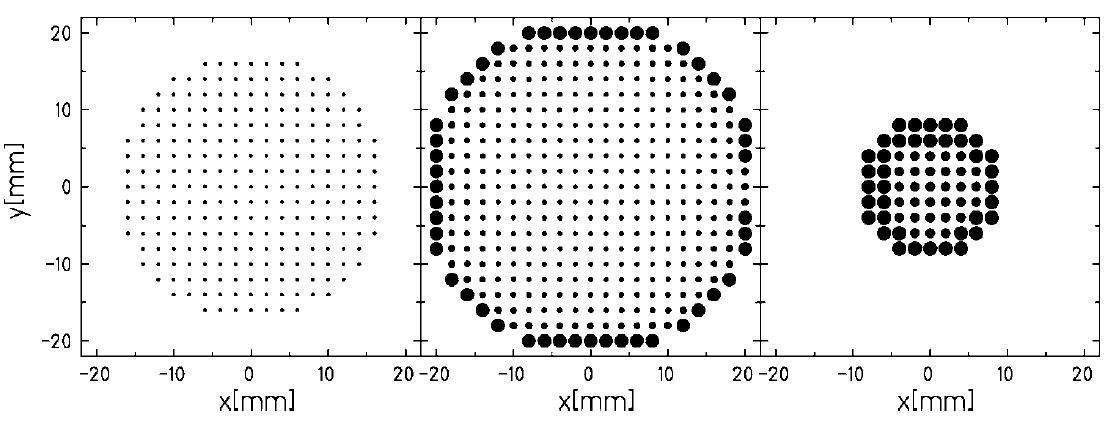
\includegraphics[scale=0.4]{./teile/introduction/inhomo.png}
\caption{Particle fluence distribution depending on the IES, starting with the most distal one (left) and moving to more proximal regions. 
Figure taken from \cite{Krae00}}
\label{inhomo}
\end{center}
\end{figure}

% \vspace*{-1cm}

\subsection{Organ motion in radiotherapy}

Many target sites are influenced by temporal changes. Depending on the underlying mechanism, one distinguishes patient positioning 
related organ motion and organ motion in-between treatment fractions (interfractional motion) or during a treatment 
application (intrafractional motion). The different organ motion types will be specified in this section. Furthermore motion acquisition 
strategies as well as techniques to overcome the motion influence, so called motion mitigation techniques, will be presented. Finally an 
overview over the treatment planning workflow including motion (four dimensional - 4D) will be given. 

\subsubsection{Motion types}

An overview of the different organ motion types is given by Langen and Jones \cite{Lan01}. Three main categories can be determined: 
patient positioning related motion, interfractional motion and intrafractional motion. Examples of these different motion types can be seen 
in figure \ref{motion}. It should be noted that all motion types can occur in a patient. Thus when dealing with intrafractional motion, 
interfractional motion as well as patient positioning needs to be accounted for.\newline
\newline
\textbf{Patient positioning} can cause changes in tumor shape as well as uncertainties in the tumor position. A difference in positioning 
between image acquisition (e.g. CT) and treatment delivery may introduce systematic displacements and hence threaten the outcome of the 
treatment. Patient fixation systems and dedicated protocols are applied to overcome this motion influence. Stereotactic fixation with e.g. 
masks are used on a daily basis. The other two motion types however are purely internal and are distinguished according to the time scale 
they occur on.\newline
% \newline
\newpage
\textbf{Interfractional motion} occurs within hours and days, hence between two treatment sessions (if multiple fractions 
are applied). Anatomical changes caused by interfractional motion are manifold. Prostate cancer patients are often subject to position 
changes due to varying gut and bladder fillings \cite{Fok04}. For lung cancer patients, changes in the breathing pattern are troublesome. 
Sonke et al. \cite{Son08} reported that even though the respiratory motion trajectory is often reproducible, the baseline of the tumor 
motion can vary significantly. Cancer patients in general are also subject to tumor shrinkage \cite{Mor09} in the course of the treatment. 
In order to mitigate interfractional motion, repeated imaging needs to be carried out.\newline
\newline
\textbf{Intrafractional motion} occurs on a time scale of seconds to minutes. The main reason for intrafractional motion are respiration 
and heart beat. Even though the exact motion patterns varies from patient to patient, it can be stated that breathing is a quite regular 
and slow process, with a rather big amplitude. Heart beat on the other hand has a smaller amplitude compared to respiration, but it is a 
high frequency motion with 60 to 80 heart beats per minute compared to 10 to 20 respiration cycles in the same time. These two motions 
superimpose and the influence of both will be studied in the framework of this work when targeting sites in the heart. Different motion 
mitigation techniques for intrafractional motion will be presented in a seperate subsection. 

\begin{figure}[H]
\begin{center}
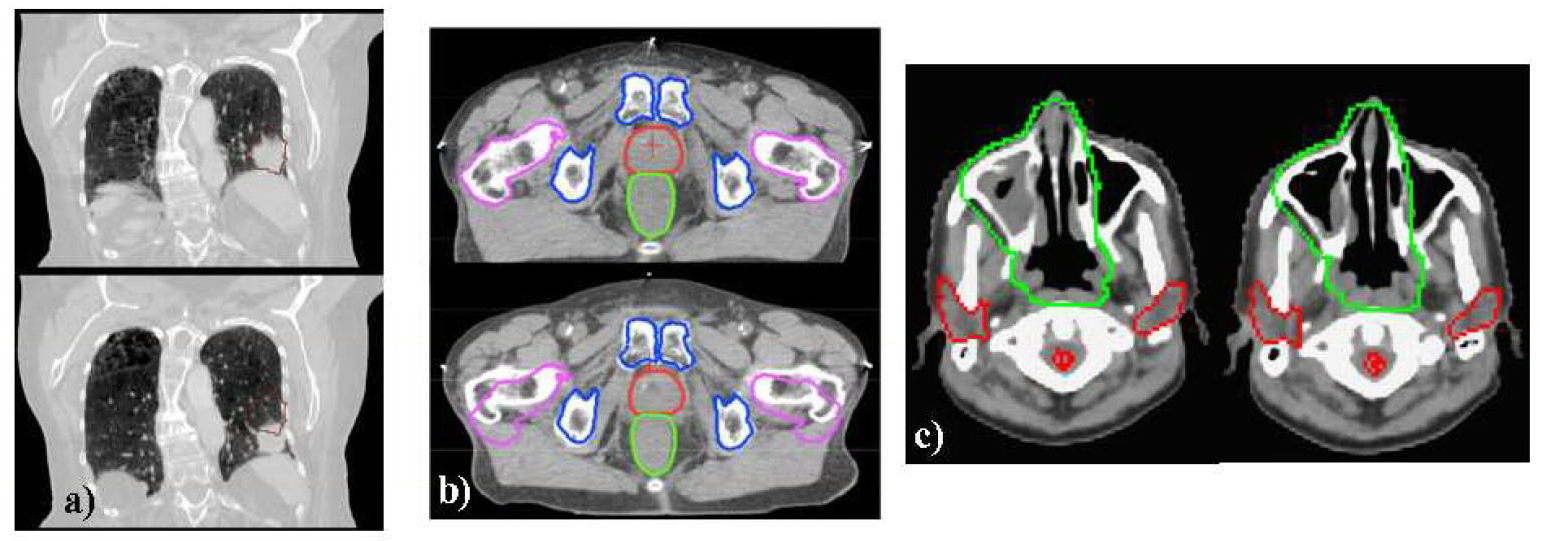
\includegraphics[scale=0.43]{./teile/introduction/motion_examples.png}
\caption{Examples of the three major motion categories. On the left side (a) a lung tumor is displayed, which moves due to the respiration 
of the patient (intrafractional motion). Interfractional position changes are examplary shown in the middle (b), where two CT scans of a 
prostate patient are compared. Density variations between two CT scans are shown in (c). Figure taken from \cite{Eng11}}
\label{motion}
\end{center}
\end{figure}

\subsubsection{Motion acquisition}
\label{Motionacq}
For a successful irradiation of the moving target, the intrafractional motion of the target site must be known during the treatment process. 
This is for example achieved by time resolved computed tomography scans (4D-CTs) and the potential usage of online motion measurement.\newline
\newline
For the acquisition of 4D-CT scans the motion signal is recorded during the imaging. The motion cycle is then divided into $N$ quasi-stationary 
sections (so-called motion phases (MP)). In every MP a full regular CT scan is reconstructed. In order to achieve this data is recorded in every 
slice for a whole motion cycle. By correlating the data gained from the motion signal with the recorded CT information, the 
scans are afterwards rearranged according to their affiliation to a certain MP. For more information on 4D-CTs the reader is refered to 
e.g. \cite{Rie05}.\newline
\newline 
A review of the different motion detection techniques can be found at \cite{Eva08}. 
One distinguishes between direct measurement techniques and surrogate signals. Examples for direct measurements are ultrasound and 
fluoroscopy. In fluoroscopy, the patient is irradiated with X-rays and the absorption pattern is displayed on a fluorescent screen, hence 
limiting the acquisition time of this method by the deposited dose. The monitoring time in ultrasound is not limited since no ionizing radiation 
is needed and hence a real time imaging is feasible \cite{Pra12}. Nevertheless influence of air limits the resolution and thus raises 
difficulties when being applied in the thorax region of the patient. Surrogate signals detect variables which are directly related to the 
source of organ motion. Examples of these kind of techniques for respiration are methods which correlate the movement of the torso to the 
phase in the respiration cycle. One possibility is to monitor the height of the patient surface with camera systems or laser 
displacement sensors or additionally using infrared markers attached to the patient's body \cite{Tad98, Ber05, Schw04, Ser13}. 
Alternatively the volume of the torso can be measured by using a belt-like strain gauge \cite{Li06}. Other approaches measure e.g. the airflow 
of the patient \cite{Kub96, Hanl99}.\newline
\newline
Combinations between direct measurement techniques and surrogate signal acquisition exist and are e.g. used in the 
Cyberknife system. Their Synchrony system (see also \ref{cardiacradiosurgery}) combines fluoroscopy (direct) with an infrared camera 
system (surrogate). This offers the advantage of a drastically reduced fluoroscopy acquisition time as it is only used to check and 
update the surrogate system \cite{Sha10, Lue12}.

\newpage

\subsubsection{Motion mitigation techniques for intrafractional motion}

% In conventional radiotherapy and passive particle therapy, moving targets are treated by enlarging the safety margins to the target region 
% (irradiating the ITV, which encompasses the target motion - see sections before). A homogenous dose distribution is thereby achieved. 
% In treatment modalities like IMRT and 
In particle beam scanning the beam delivery interferes with the intrafractional target 
motion, causing local over- and underdosages in the target volume, an effect known as Interplay \cite{Phi92, Ber08, Ber12, Loe13}. 
The exactly resulting interplay pattern is dependent on many different factors, like the beam direction, the scanning speed, the motion 
amplitude and starting phase etc. Thus techniques which mitigate the influence of the underlying target motion have to be applied. The three 
main techniques (rescanning, gating and tracking) will be explained in more detail.\newline
\newline
\textbf{Rescanning}, also known as repainting, is a specific approach for beam scanning and based on statistical averaging of different 
interplay patterns \cite{Phi92, Rie10}. Scanning the target $N$ times with a reduced dose of $\mathrm{1}/\mathrm{N}$ results in a 
Gaussian distributed dose around the theoretically intended one (see figure \ref{rescanning}). As the variance of the distribution is proportional 
to $\mathrm{1}/\mathrm{\sqrt{N}}$ the result will be better the more rescans are used. The technical realisation of rescanning is easier than 
for e.g. gating and beam tracking, 
especially as it does not require real-time motion monitoring, and results in a homogeneous dose to the inner region of the target when 
using enough rescans $N$. Anyhow it can lead to an increased dose deposition to the surrounding, normal tissue and to under dosages in 
the outer part of the target volume. So far rescanning has not been used in patient treatments, but certain centers (e.g. NIRS \cite{Fur07}) 
and PSI \cite{Zen10}) plan it for the future.

\vspace*{-0.4cm}

\begin{figure}[H]
\begin{center}
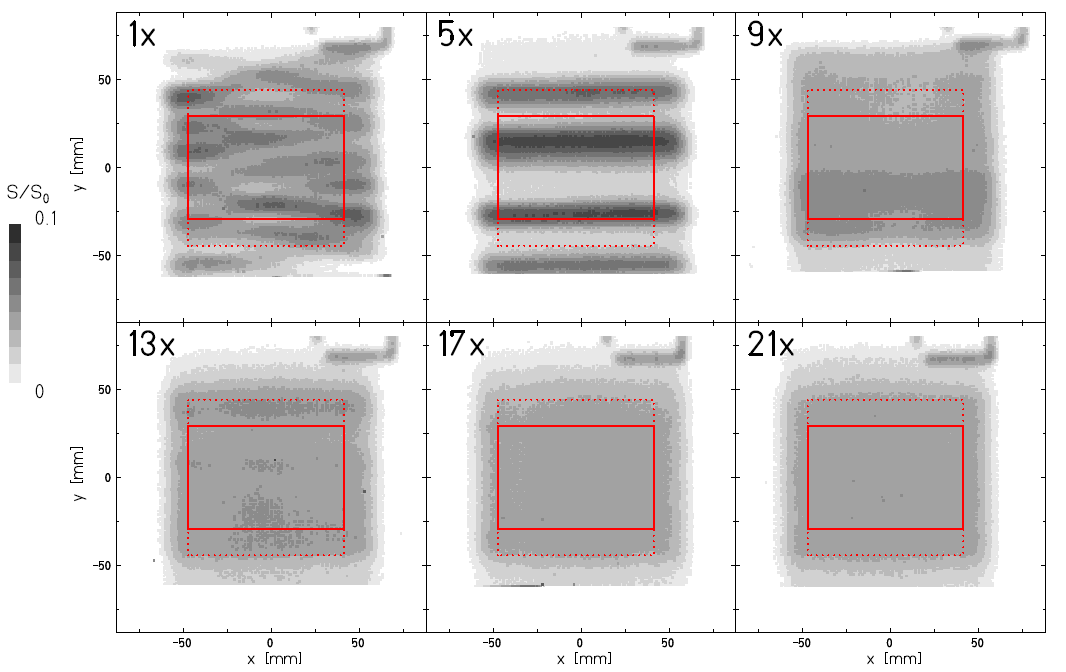
\includegraphics[scale=0.45]{./teile/introduction/rescanning.png}
\caption{Principle of rescanning in film irradiations. Averaging multiple interplay patterns leads to a homogeneous dose in the target area 
(solid red square). Figure taken from \cite{Ber09b}. }
\label{rescanning}
\end{center}
\end{figure}

\textbf{Gating} is the interrupted irradiation of the target during a selected part of the motion cycle, the gating window \cite{Kub96, Min00} 
\cite{Li06} (see figure \ref{gating}). Typically a gating window around the most reproducible motion states are chosen, which show a comparably 
small motion (e.g. end exhale in case of respiration). This technique is also used for passive beam delivery, as it reduces the size 
of ITV margins. In the gating window a small motion, the so-called residual motion, remains. In case of beam scanning this can result in 
small interplay effects. Different approaches are studied to overcome this drawback \cite{Fur07, Zen10, Ber09}. Gating requires 
online motion monitoring and prolongs the treatment time. For centers with passive beam delivery gating has already been successfully 
used \cite{Min00, Iwa10, Has06}.

% \vspace*{-0.6cm}

\begin{figure}[H]
\begin{center}
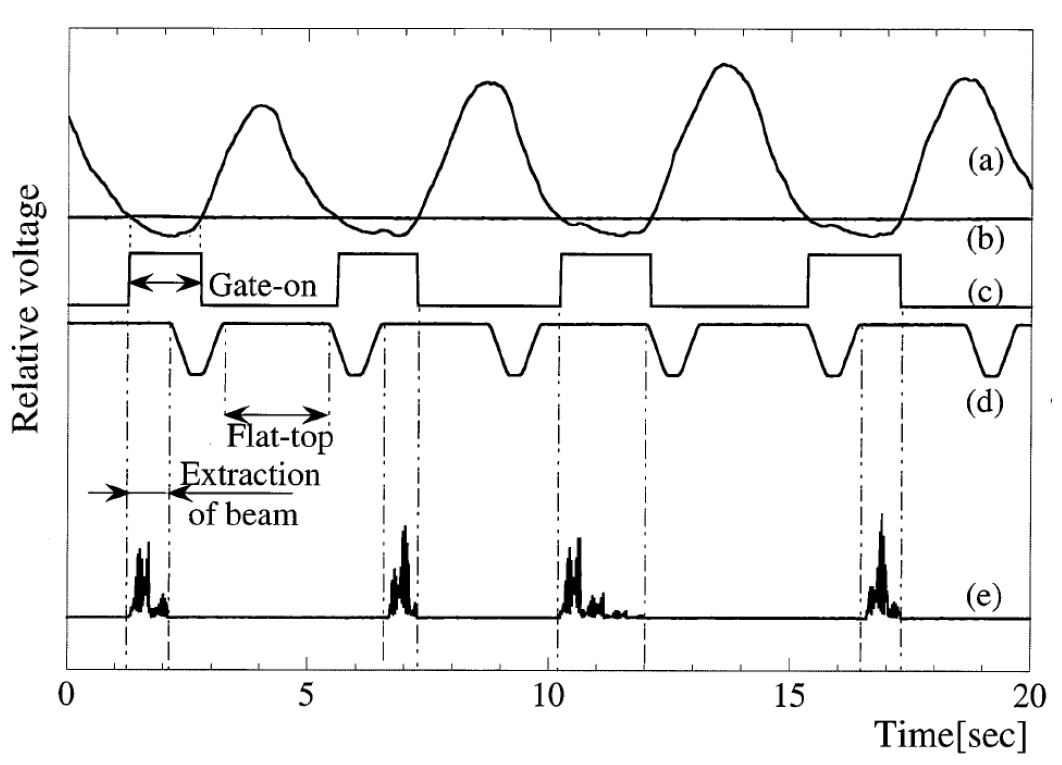
\includegraphics[scale=0.45]{./teile/introduction/gating.png}
\caption{Principle of gating. Line (a) is the respiratory signal. At end exhale the gradient of the respiration is flat, enabling an 
irradiation without large effects of the target motion. The beam (c) is thus only applied during this time. The gating window is activated 
as soon as the respiratory motion crosses line (b). Figure taken from \cite{Min00}}
\label{gating}
\end{center}
\end{figure}


\textbf{Beam tracking} of organ motion requires the adaptation of the beam position to the target motion in real time. It was originally proposed 
for IMPT \cite{Kea01} and ideally requires no additional margins, nor prolongs the treatment time. Prerequisite of this method is a fast beam 
delivery system. Tracking is clinically used in the Cyberknife Synchrony system (see section \ref{cardiacradiosurgery}). 
In comparison to photon irradiation, tracking with particles needs a careful consideration and adaptation of longitudinal changes due to 
the Bragg Peak structure of ions. The implemented tracking system at GSI \cite{Gro04} uses fast deflecting dipole magnets, which 
are also used for beam scanning for the lateral adaptation of the beam. The longitudinal changes are accounted for by two polymethyl 
methacrylate (PMMA) wedges, which are mounted on a fast, linear stepmotor close to the target (see figure \ref{tracking}) \cite{Sai09}. By 
changing the relative distance between the wedges, the beam penetrates PMMA with different thicknesses, thereby changing its energy and 
hence range. Even though the high precision of the system has been proven \cite{Ber07, Ber10, Sai09} a clinical use 
is not feasible yet due to the lack of fast and precise real-time internal motion monitoring that includes partical range information.

\begin{figure}[H]
\begin{center}
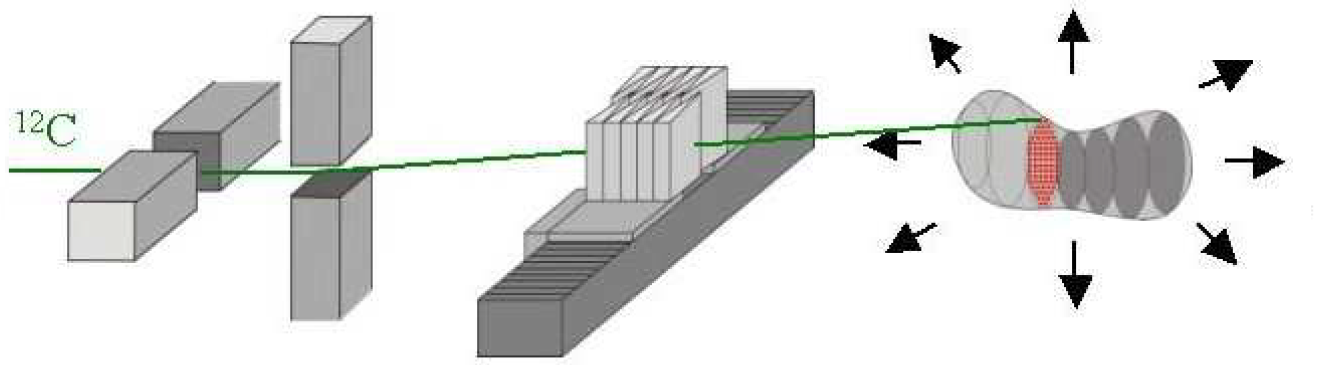
\includegraphics[scale=0.4]{./teile/introduction/tracking.png}
\caption{Principle of tracking at GSI. The lateral deflection is achieved via dipole scanner magnets. For the longitudinal adaptation two 
PMMA wedges are mounted on step motors, enabling to change the depth the particle beam has to traverse. Figure taken from \cite{Gro04}}
\label{tracking}
\end{center}
\end{figure}

Besides these major motion mitigation techniques, different combinations are currently studied. A combination between rescanning and 
gating is e.g. studied by Furukawa et al. \cite{Fur07} or Seco et al. \cite{Sec09} and a combination of rescanning at tracking 
by van de Water et al. \cite{Wat09}.\newline
\newline
As breathing is the main reason for intrafractional motion in most radiotherapy applications, many different other techniques have been 
investigated to directly mitigate the influence of respiration. An example is abdominal pressure, which has been used in lung 
and liver cancer patients in treatments with photons \cite{Neg01, Hof03} and recently also for scanned carbon ions at HIT (treatment 
of hepatocellular cancer \cite{Com11}). Jet ventilation \cite{Hof03} and apneic oxygenation \cite{RPTC12} are also used to partially or 
completely suppress respiration of the patient. 


\subsubsection{4D Treatment planning at GSI}

In order to account for intrafractional organ motion, time-resolved (4D) treatment planning is needed. The underlying data as well 
as the techniques for 4D treatment planning will be presented for the special case of scanned carbon ion beams at GSI.\newline
\newline
As in the static case, treatment planning for ions is based on CT scans. In the special case of 4D treatment planning, these CT scans are 
time resolved (\textbf{4DCT}s, see section \ref{Motionacq}, Motion acquisition). In order to use the information stored in the 4DCT, an \textbf{image 
registration} needs to be performed. With this a voxel-to-voxel mapping between the reference phase of the 4DCT and all other motion phases is 
gained, hence yielding a spatial correlation between the individual CT phases \cite{Ric13}. Usually, rigid and deformable registration 
methods are distinguished. While rigid registration only contains linear transformation of the original object in all three room dimensions, 
deformable registration also accounts for compression. 
Brock et al. \cite{Bro10} published a multi-institutional study where the accuracy of some of the available registration algorithms is 
presented. It can be stated that registration accuracy of most algorithms is in the order of millimeters, hence in the order of a CT 
voxel size, but is dependent on the image contrast (resulting in less accurate results when the contrast is diminished).

\begin{figure}[H]
\begin{center}
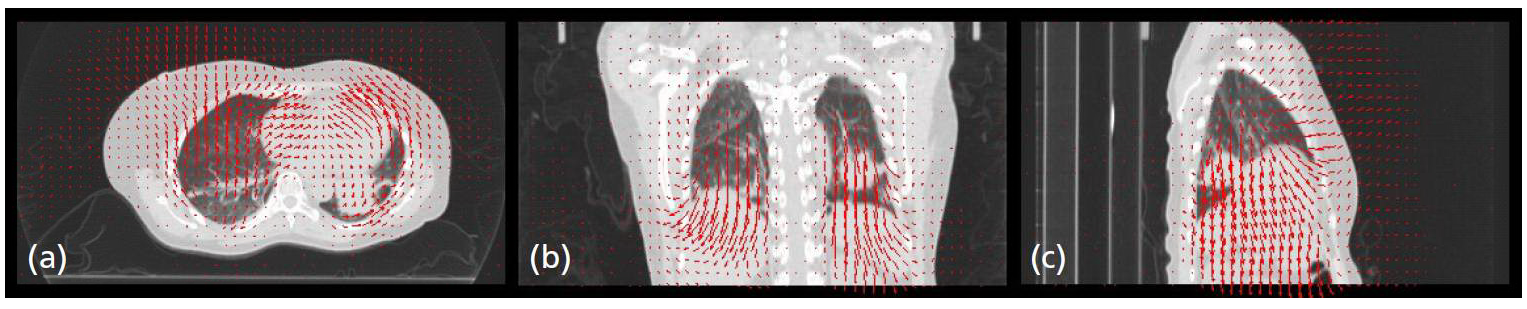
\includegraphics[scale=0.43]{./teile/introduction/registration.png}
\caption{End-exhale, 4D reference phase of a lung cancer patient with overlying deformation field to end-inhale in a) axial, b) coronal and 
c) sagittal view. Figure taken from \cite{Ric12}.}
\end{center}
\end{figure}

\vspace*{-0.8cm}

\textbf{4D treatment planning} at GSI is carried out with the in-house software \textbf{TRiP4D}. It was mainly developed by Daniel Richter \cite{Ric13} and 
is based on TRiP98 as well as a predecessor program developed by Bert and Rietzel \cite{Ber07b} together with the biological implementation 
under influence of target motion by Gemmel et al. \cite{Gem11}.  
TRiP98 was developed for static target regions and was successfully applied in the GSI pilot project \cite{Krae10, Krae00, Krae00b}.  
It is a command-line-based software without graphical interface which runs on an IBM AIX operating system and is written in C 
programming, using a pseudo object-oriented structure. For a detailed description of TRiP4D functionalities as well as of the software 
design and experimental verification the reader shall be referred to \cite{Ric13}. However, a short overview of some of the most important 
functionalities will be given here.\newline
\newline
The \textbf{4DCT structure} was implemented as a sequence of 3DCTs with a distinguished reference CT on which the dose optimization 
process is carried out. Thus the existing 3D functionalities, like the computation of water-equivalent path lengths, could be reused. 
Individual phases of the 4DCT are indexed by their position in the motion cycle. 
TRiP4D does not include native \textbf{image registration} functionalities but rather integrates and processes image registration output, obtained e.g. 
with the open source software package Plastimatch \cite{Sharp07}. The resulting deformation maps need to be obtained in two directions 
(reference-moving and moving-reference) as certain steps of the treatment planning like contour propagation require the inverse deformation 
maps.
\textbf{Contours segmentation}, of target volumes as well as organs at risk, is stored as a volume dataset model, based on the 3D 
segmentation module of TRiP98 with planar polygons on axial CT slices. Based on this 4D segmentation functionality ITVs (see section \ref{tp}) 
can be created, which are needed for certain motion mitigation 
techniques like e.g. rescanning. In general, the 4D treatment plan generation and \textbf{dose optimization} is very dependent on 
the employed motion mitigation technique. For the ITV concept \cite{Gra12}, and hence in motion mitigation techniques where the dosimetric 
effects caused by interplay are compensated but not the target motion itself, dose optimization is carried out on the 4DCT 
reference phase \cite{Ric13}. For beam tracking on the other hand additional optimization is carried out, as motion compensation vectors have 
to be computed. Furthermore 4D optimization techniques (which include the target motion for optimization by using the full 4DCT dataset, the 
vectors from image registration as well as 4DVOIs for dose optimization \cite{Gra13, Ele12}) can be developed and applied with TRiP4D.   
Based on the predecessor program of Bert and Rietzel the \textbf{treatment plan} is then split into quasi-static sub-plans 
where the raster points and the corresponding intensities are divided according to the motion phase they shall be irradiated in. 
For the overall \textbf{4D dose calculation} in TRiP4D, the sub-plans are then collected over all motion states for each dose voxel. Thereby 
the voxel position is transformed according to the deformation maps and by accounting for the radiological density distribution of 
the respective phase of the 4DCT. The total physical dose results as a summation of the dose distribution from all motion states in 
the reference state (see figure \ref{TRiP4Ddose}).  For the biological dose calculation the particle and energy spectra are also accumulated 
over all motion states and used as input for the local effect model (LEM) to calculate the RBE \cite{Scho94, Scho96, Gru12}. 
TRiP4D was extensively tested and verified in numerous experiments \cite{Ric12, Ric13}.  

\vspace*{-0.3cm}

\begin{figure}[H]
\begin{center}
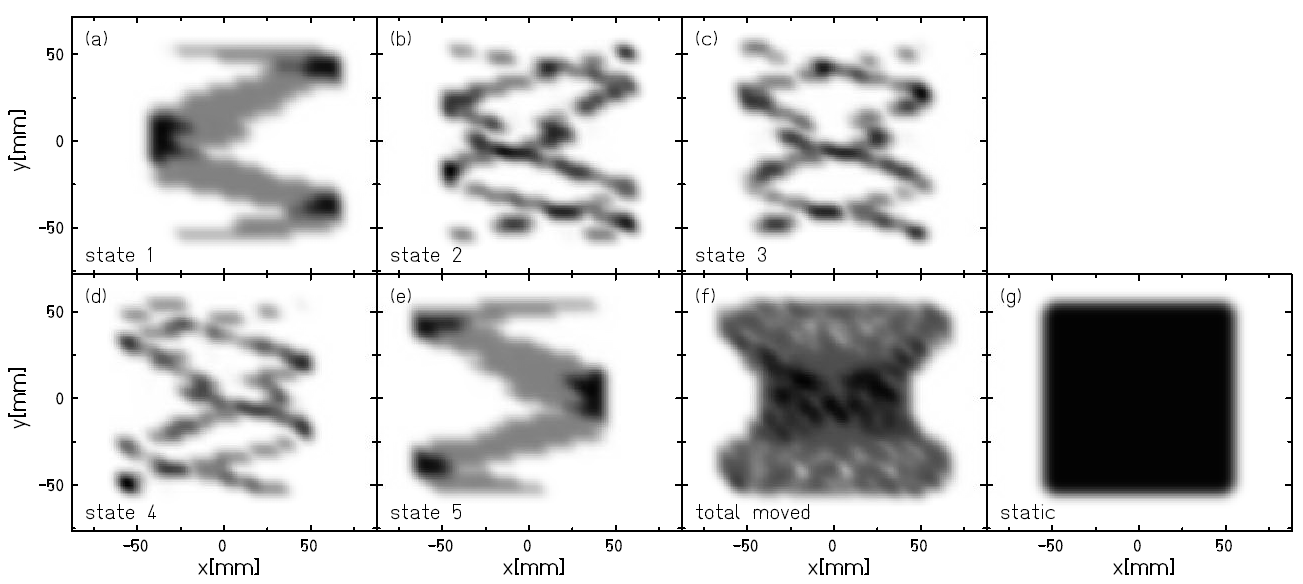
\includegraphics[scale=0.35]{./teile/introduction/4DtreatmentPlanning.png}
\caption{Resulting film response in experimental validation of 4D dose calculation with TRiP4D. Images a)-e) show the individual dose 
deposition in each of the five motion states. In f) the total dose deposition in 4D is displayed. On the stationary film in g) a homogeneous 
dose is deposited in 3D. Figure taken from \cite{Ric12}}
\label{TRiP4Ddose}
\end{center}
\end{figure}



\newpage

%%%%%%%%%%%%%%%%%%%%%%%%%%%%%%%%%%%%%%%%%%%%%%%%%%%%%%%%%%%%%%%%%%%%%%%%%%%%%%%%%%%%
\section{Atrial fibrillation}

Atrial fibrillation (AF) is the most common cardiac arrhythmia. It occurs in $\sim$2\% of the population older than eighty in Europe 
and the US, leading to over six million patients in Europe \cite{ESC10} and over two million patients in the United States \cite{CE09}. The 
lifetime risk of developing AF is $\sim$25\% for people over forty. Since age is an important risk factor for this cardiac arrhythmia the 
prevalence is estimated to double in the next fifty years due to ageing of society (see figure \ref{USincidences}).\newline

\begin{figure}[H]
\begin{center}
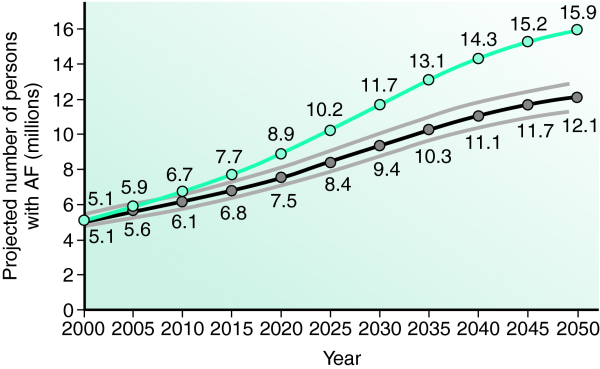
\includegraphics[scale=3]{./teile/introduction/af_incidences_us.png}
\caption{Trend of AF incidences. The black curve indicates the projected number of patients assuming no further increase in age-adjusted AF 
incidences. The green curve represents the trend assuming a continuous increase in incident rates as evident in 1980 to 2000. Figure taken 
from \cite{Miy06}}
\label{USincidences}
\end{center}
\end{figure}

Even though in itself not life threatening, it alters the quality of life and increases the risk to suffer a stroke. It is 
estimated that the stroke risk in AF patients is 5-fold higher \cite{Ben98, Wol91}. AF often remains undiagnosed 
(silent AF). It is stated that one out of five acute strokes is attributed to AF \cite{ESC10}. Other late effects and related events 
include cognitive dysfunctions like vascular dementia and impairment of left ventricular function. In general death rates are stated to 
approximately double by AF \cite{ESC10}, leading to a ten year survival rate of 25\% compared to 46\% in patients with a normal sinus 
rhythm (age ranged from 14 to 73 years with a median of 42 years) \cite{Oles62, ACC06}.\newline
\newline
In the following the normal signal propagation through the heart's conduction system will be explained in order to contrast the occurring 
differences in AF. Possible causes for AF and underlying risk factors as well as current treatment modalities will be presented.

\newpage

\subsection{Heart's conduction system}
\label{HCS}
The conduction system of the heart controls the generation and propagation of electrical signals, so called action potentials, that cause 
the heart muscle to contract and hence to pump blood \cite{Med}. The small electrical activity of the action potentials is measurable at the 
surface of the body, enabling a graphical record with an electronic recording instrument, the Electrocardiograph (ECG). In the following the 
events during a single heart beat and the corresponding detection in an ECG (see fig. \ref{ecg}) will be explained. 
The action potentials can originate spontaneously in any of the specialized cardiac muscle cells which form the conduction system. In a healthy 
heart each beat begins in the right atrium with an action potential from the sinoatrial (SA) node (see fig. \ref{condsys}), making it the 
natural pacemaker of the heart. The signal then spreads across both atrial chambers causing the muscle cells to contract (atrial systole) 
which is represented as the P-wave in an ECG. It is followed by a period of conduction (PR-segment in ECG) in which the signal enters the 
ventricles via the atrioventricular (AV) node. As the signal spreads the ventricles contract very rapidly 
(ventricular systole), which is displayed in the QRS-complex in an ECG. Atrial activity is hidden in the ECG by the QRS complex. As the signal 
passes out of the ventricles, the ventricular walls start to relax (ventricular diastole). The T-wave marks this ventricular repolarization. 
The sequence of these events and the corresponding ECG traces repeat with every single heartbeat.\newline

% \vspace{-7cm}
% \vspace{-1.5cm}
\vspace{-0.5cm}
\begin{figure}[H]
\begin{center}
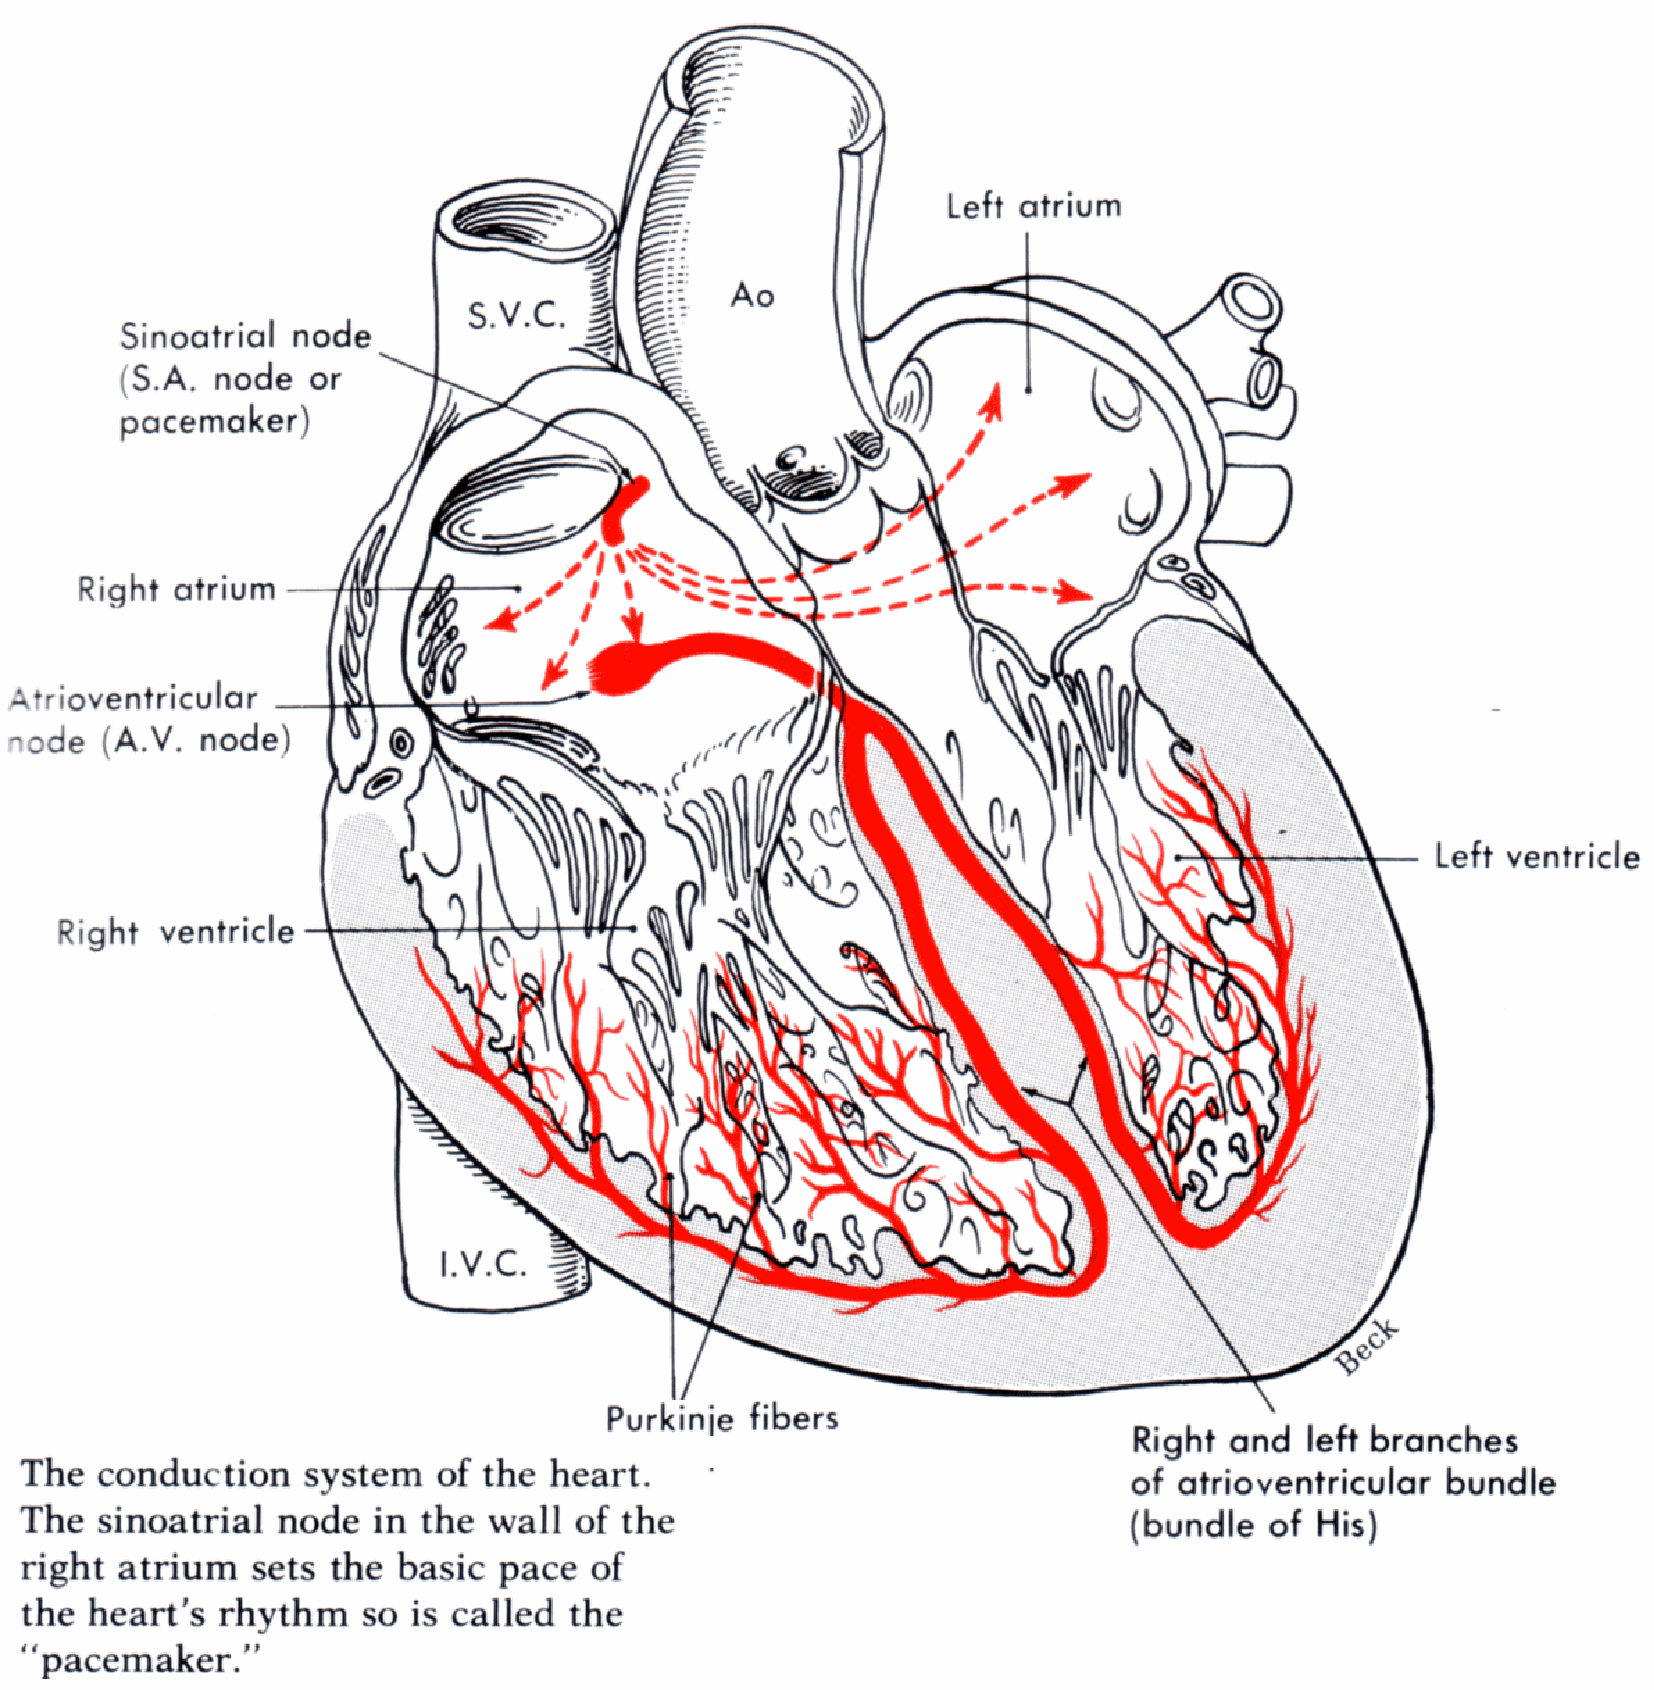
\includegraphics[scale=0.23]{./teile/introduction/conduction_system.png}
\caption{Scheme of the conduction system of the heart. Figure taken from \cite{amc}}
\label{condsys}
\end{center}
\end{figure}

\newpage

\begin{figure}[H]
\begin{center}
% 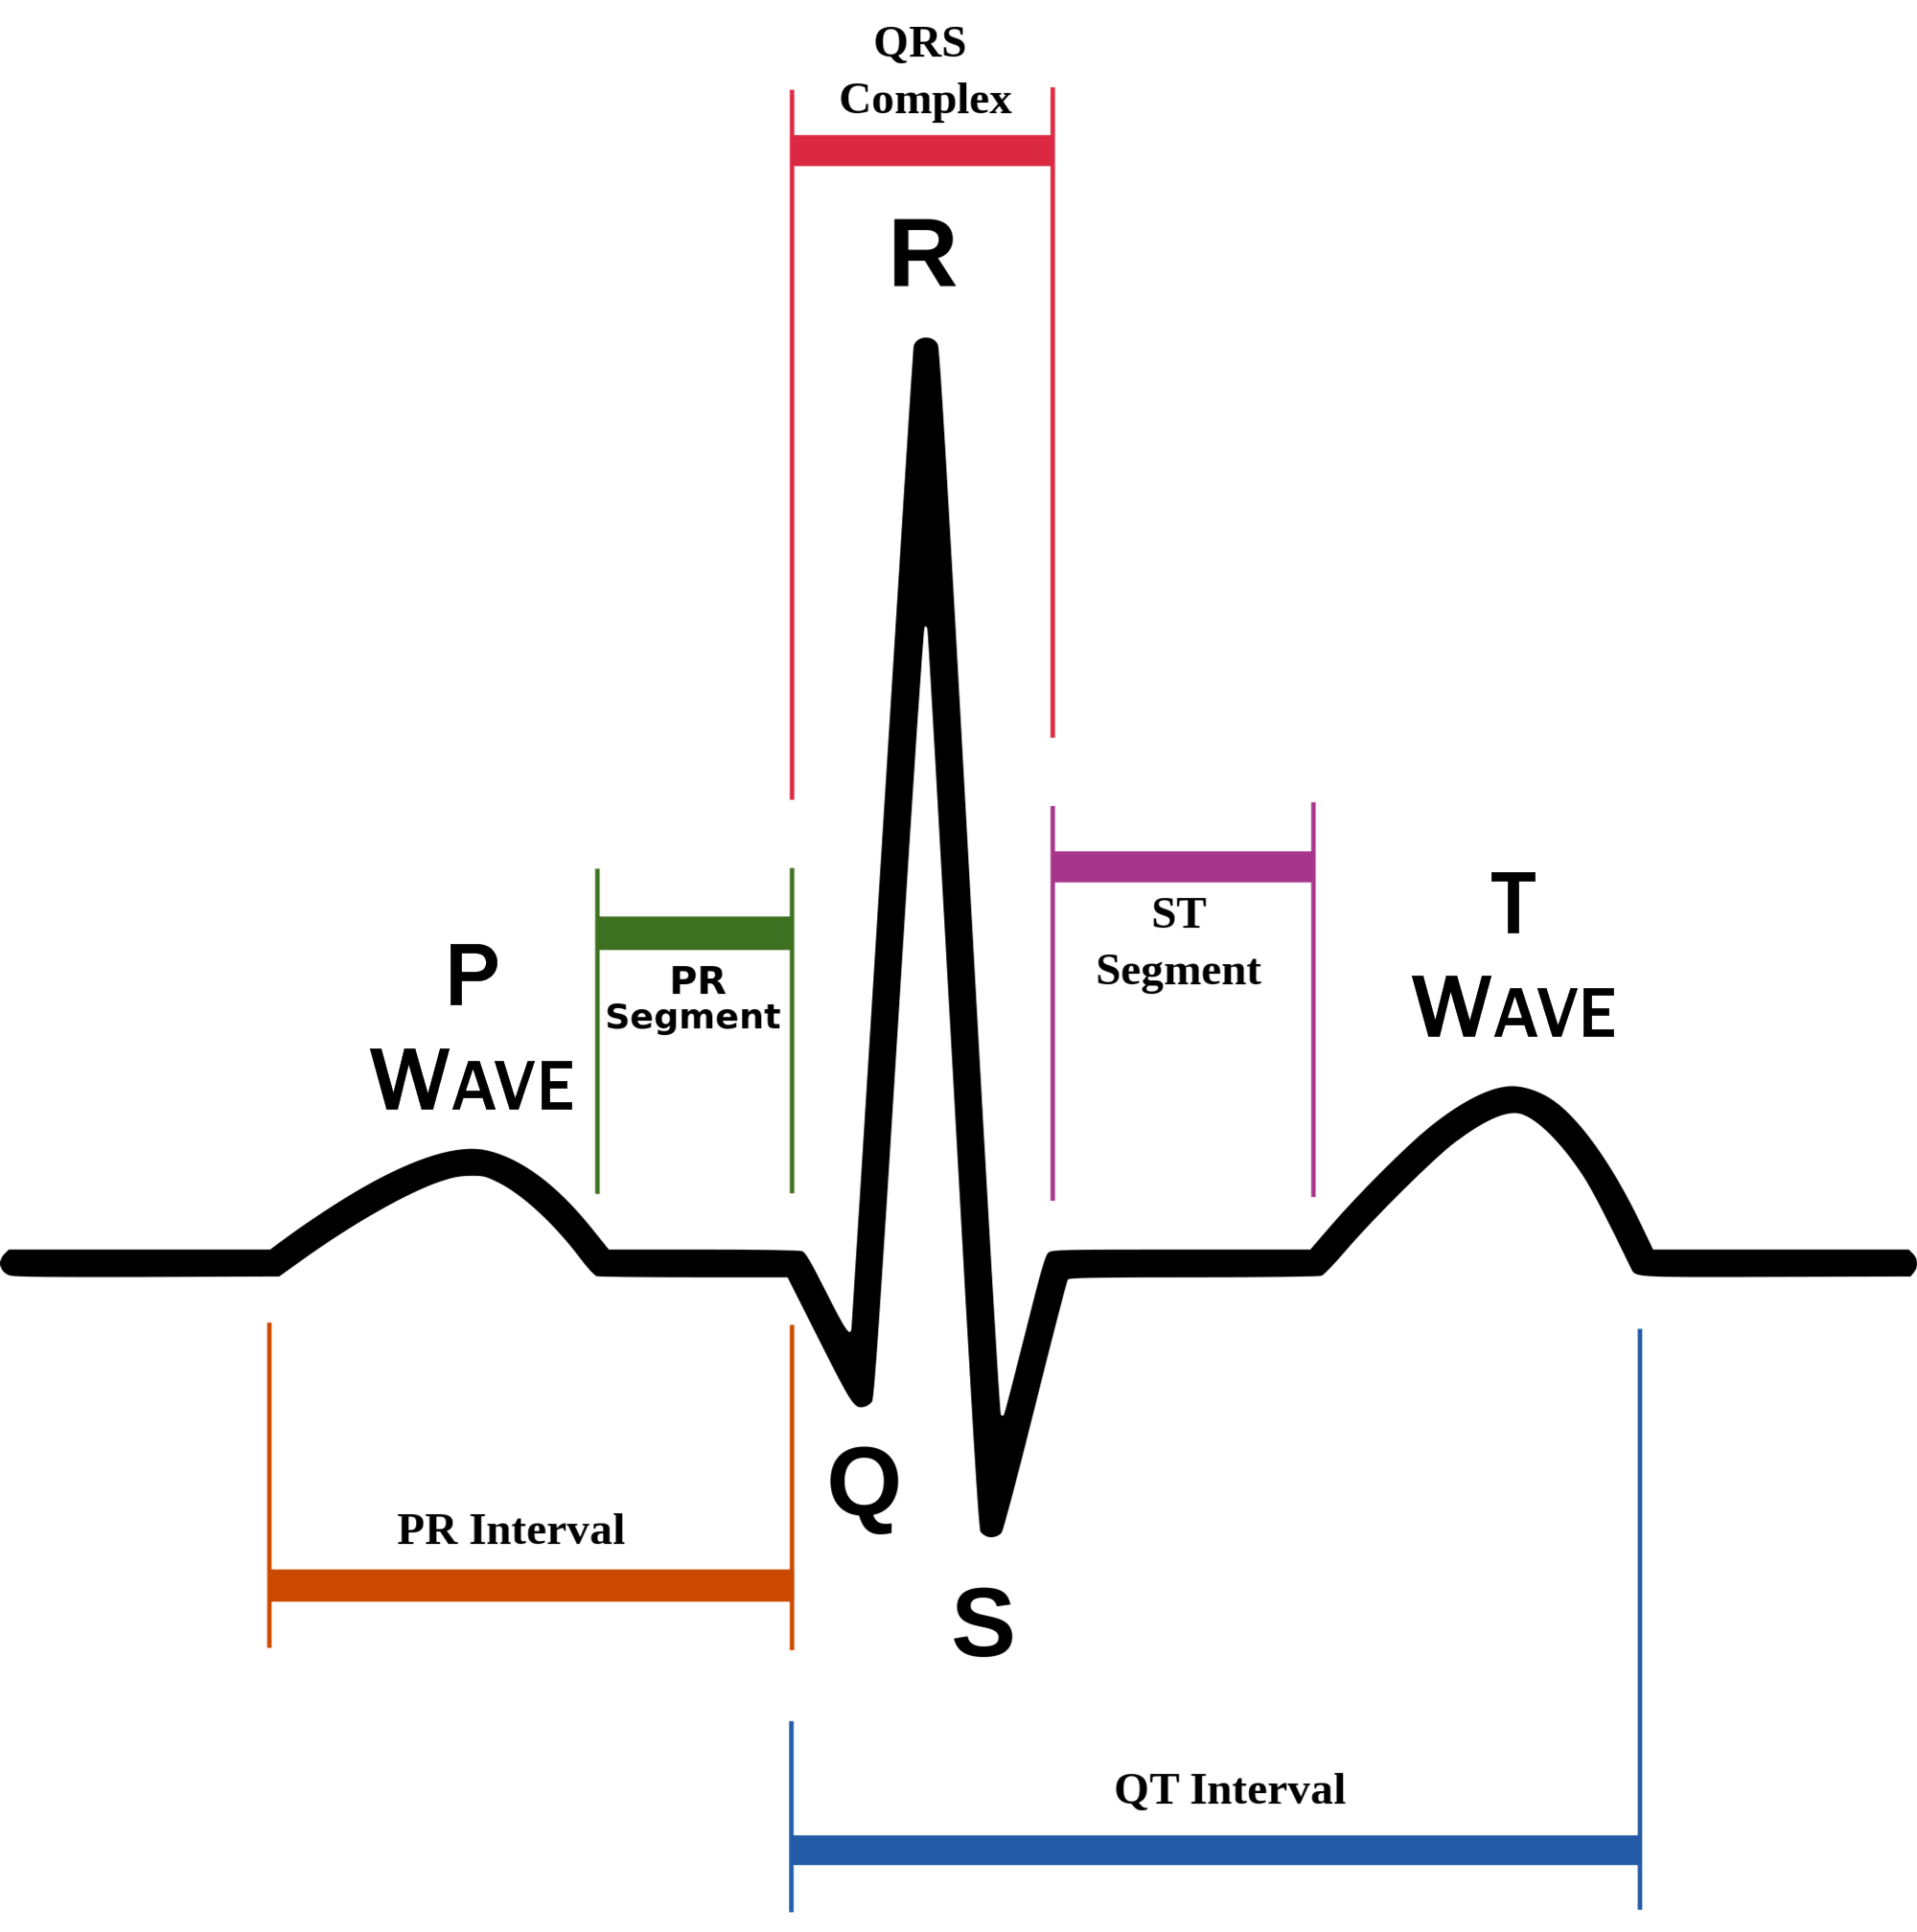
\includegraphics[scale=0.13]{./teile/introduction/ecg.png}
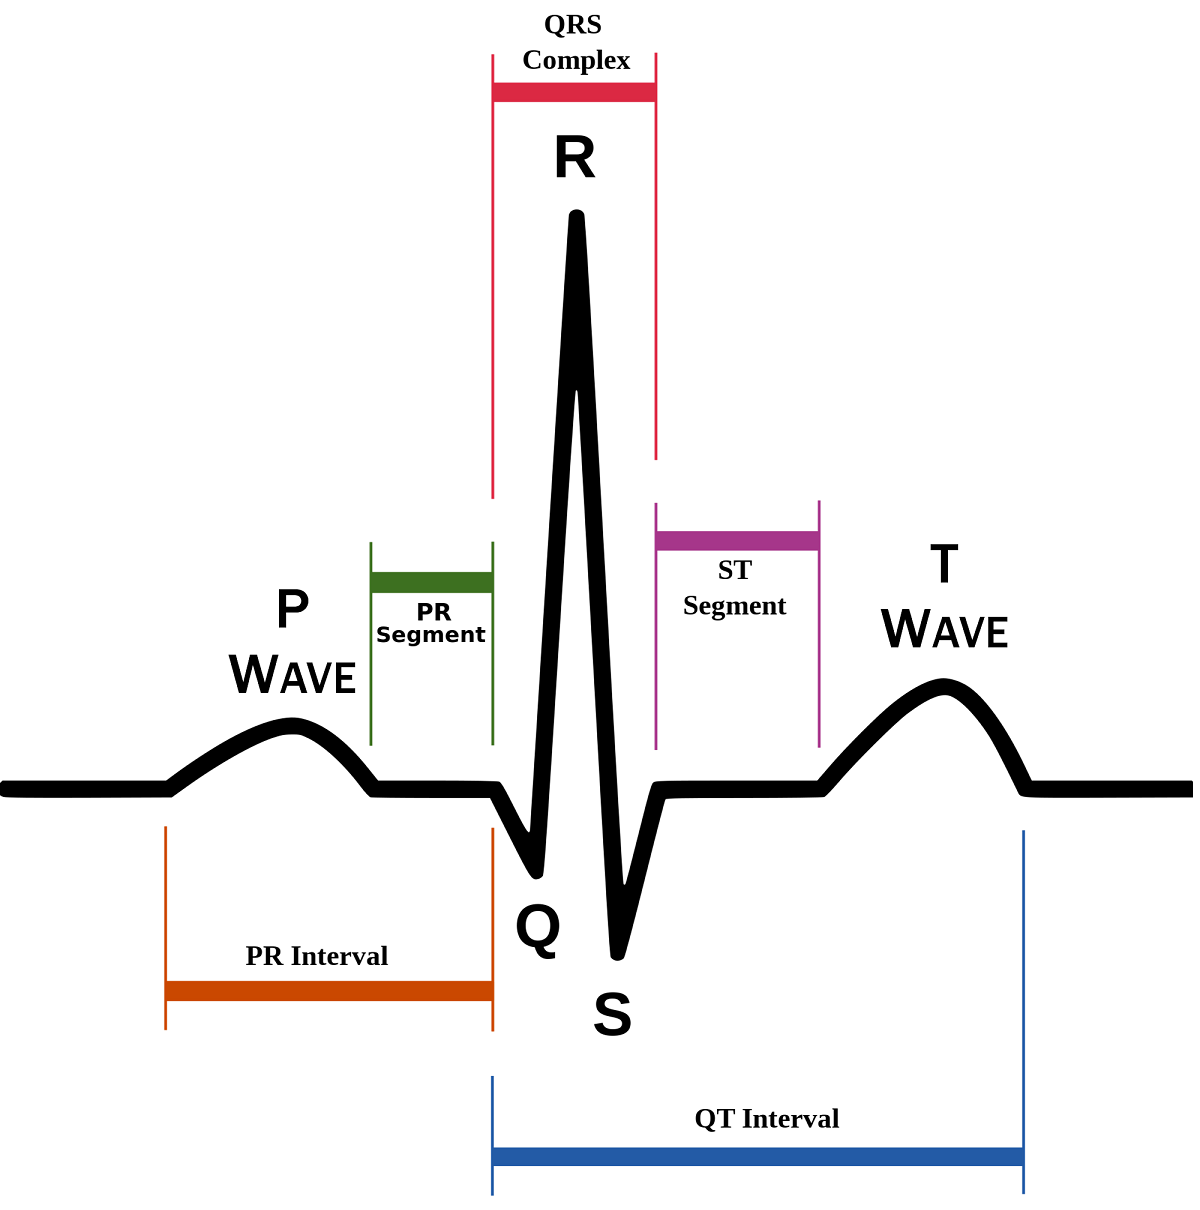
\includegraphics[scale=0.3]{./teile/introduction/ecg_2.png}
\caption{ECG trace of a normal heart beat. Figure taken from \cite{afib}}
\label{ecg}
\end{center}
\end{figure}

In AF there is unorganized atrial activity, leading to quivering motion and hence the atria are not able to sustain a healthy pumping rhythm. 
An exemplary ECG trace for AF can be seen in figure \ref{af_ecg}. 
Possible reasons and triggers for this abnormal action potential propagation are stated in the section \ref{AFriskfactor}.

\begin{figure}[H]
\begin{center}
% 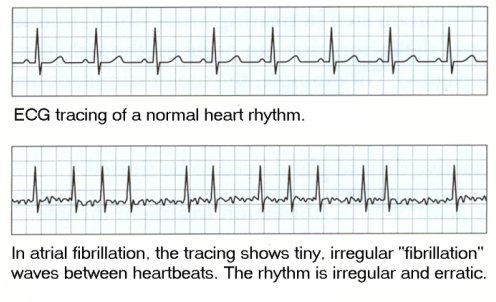
\includegraphics[scale=3]{./teile/introduction/AF_ECG.png}
\subfigure[normal sinus rhythm]{
 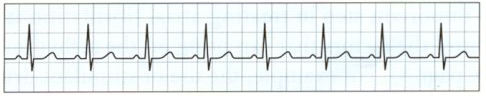
\includegraphics[scale=1]{./teile/introduction/AF_ECG_1.png}
 }
 \subfigure[AF patient]{
 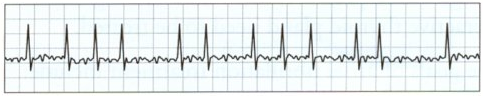
\includegraphics[scale=1]{./teile/introduction/AF_ECG_2.png}
 }
\caption{ECG traces for a normal sinus rhythm (a) and for an AF patient (b). In AF, the tracing shows small, irregular fibrillation waved 
between heartbeats. The rhythm is irregular and erractic. Figure taken from \cite{afib}}
\label{af_ecg}
\end{center}
\end{figure}

\newpage
\subsection{Types of atrial fibrillation}

Based on the duration and presentation of the condition different types of AF are clinically distinguished \cite{ESC10, CE09} (paroxysmal, 
persistent, long-standing and permanent) (see figure \ref{af_types}). Furthermore silent AF may present itself as any form of the stated AF 
types. As the name indicates, the condition is asymptomatic and hence undiagnosed. It usually manifests as an AF related complication like an 
ischemic stroke. About one third of people with AF are estimated to be unaware of their condition \cite{ESC10}.\newline
\newline
Usually AF progresses over time. Starting as short and rare episodes the condition develops into longer and more frequent attacks \cite{ESC10}.
In figure \ref{afovertime} the typical time course of AF is indicated. In the lower part of the diagram different periods of AF are shown 
(dark blue boxes). Possible treatment possibilities at the different stages of AF are shown in the upper bars. Medication uptake which should 
prevent the formation of blood clots are represented by light blue boxes. These medications are recommended in the majority of AF patients. 
The red boxes indicate system relief therapies while the grey boxes represent rate control measures.

\vspace*{0.7cm}

\begin{figure}[H]
% \begin{minipage}{0.475\textwidth}
\begin{minipage}{0.5\textwidth}
\centering
    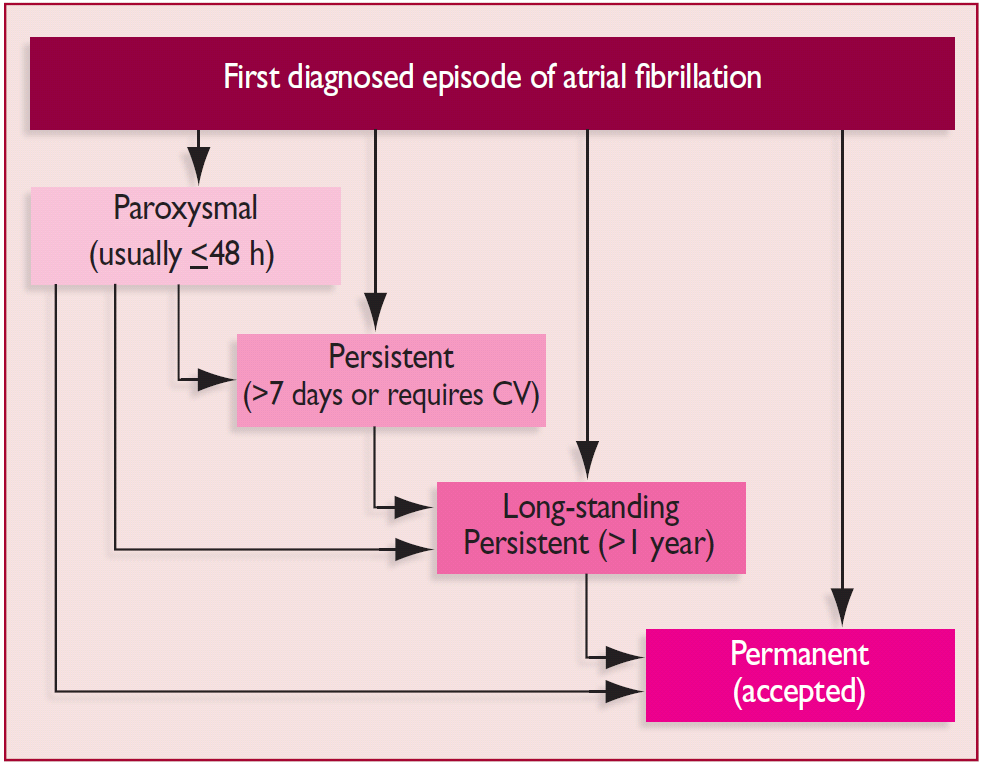
\includegraphics[width=\textwidth]{./teile/introduction/af_types.png}
    \caption{Different types of AF. Figure taken from \cite{ESC10}}
     \label{af_types}
\end{minipage}
\hfill
% \begin{minipage}{0.475\textwidth}
\begin{minipage}{0.52\textwidth}
\centering
  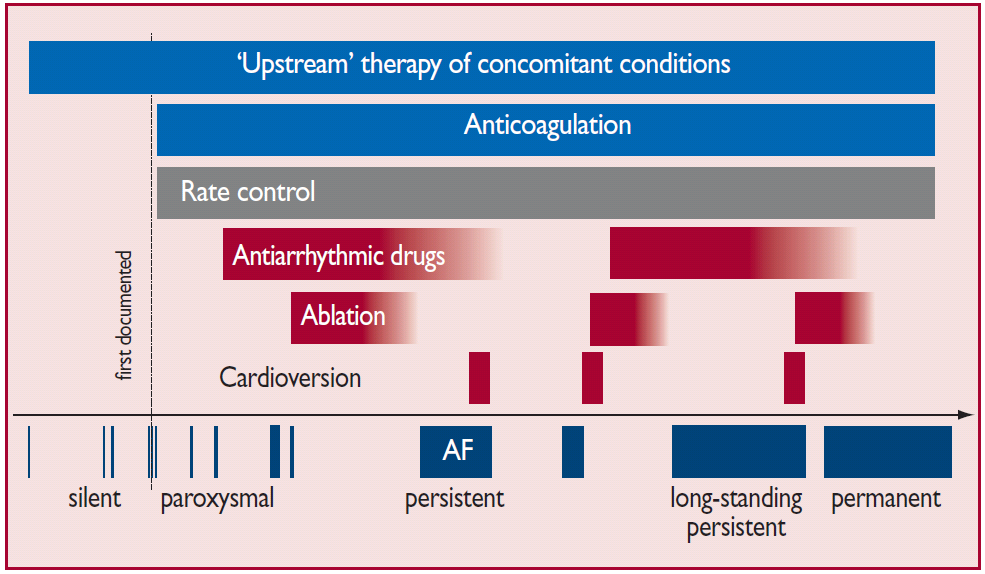
\includegraphics[width=\textwidth]{./teile/introduction/af_over_time.png}
  \caption{Typical time course of AF and potential treatment possibilities. Figure taken from \cite{ESC10}}
  \label{afovertime}
\end{minipage}
\end{figure}

  
% \begin{figure}[H]
% \begin{center}
% 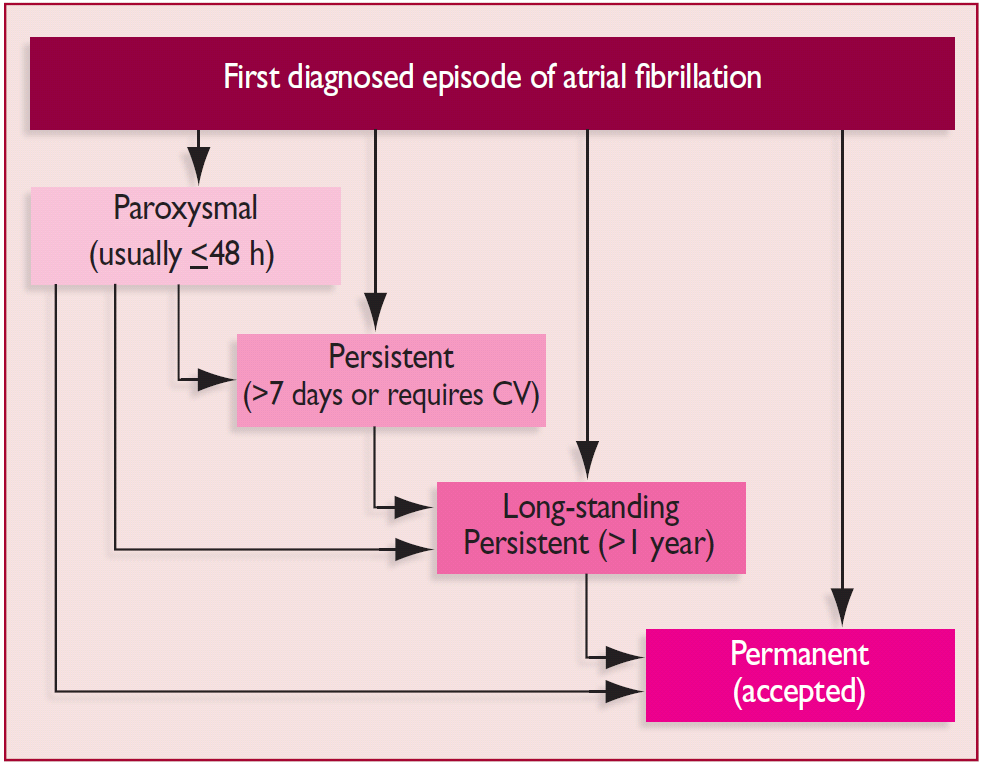
\includegraphics[scale=0.2]{./teile/introduction/af_types.png}
% \caption{Different types of AF. Figure taken from \cite{ESC10}}
% \label{af_types}
% \end{center}
% \end{figure}
% 
% 
% \begin{figure}[H]
% \begin{center}
% 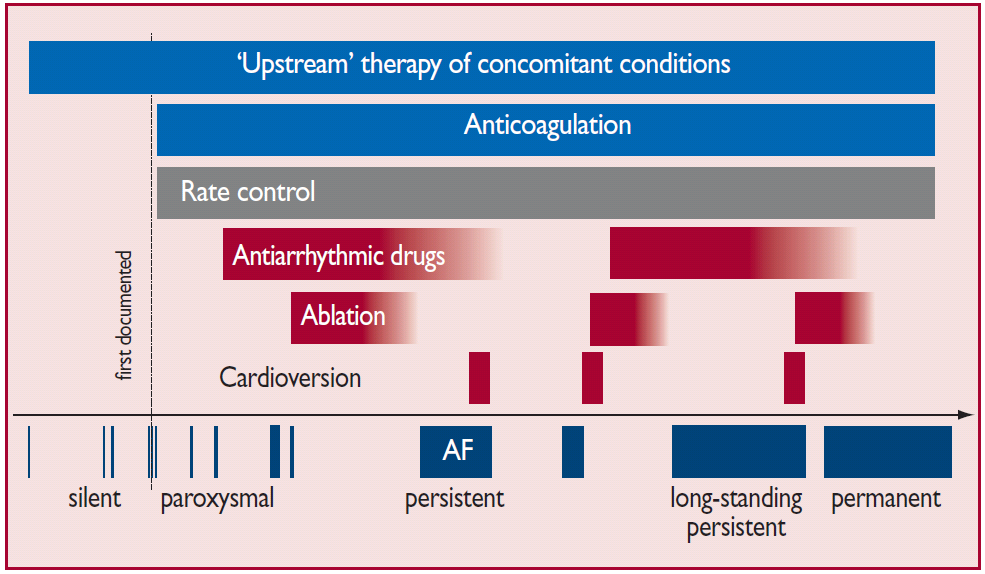
\includegraphics[scale=0.22]{./teile/introduction/af_over_time.png}
% \caption{Typical time course of AF with different periods of AF (dark blue boxes) and possible treatment 
% possibilities as well as medication uptake. Figure taken from \cite{ESC10}}
% \label{afovertime}
% \end{center}
% \end{figure}


\newpage
\subsection{Possible causes for atrial fibrillation and risk factors}
\label{AFriskfactor}

The mechanisms of AF are not yet fully understood. The multifactorial mechanisms may influence and sustain each other. 
Current research indicates that one can distinguish between focal 
mechanisms and multiple wavelets \cite{CE09}. For most patients with paroxysmal AF a localized, focal trigger can be identified. This is 
not the case in patients with persistent or permanent AF, where the multiple wavelet hypothesis is believed to be more accurate.\newline

An identified \textbf{focal trigger} site are the pulmonary veins (PVs). In the benchmark paper Ha\"{\i}ssagurre et al. \cite{Hai98} studied 
45 patients with frequent episodes of AF ( (344 $\pm$ 326)minutes episodes per 24 hours) finding ectopic beats\footnote{beats which arise 
from cells outside the region in the heart muscle ordinarily responsible for impulse formation} originating from the pulmonary veins in 
94\% of the cases. The underlying mechanism why PVs become arrhythmogenic in some patients while it remains dormant in others is 
still not clear \cite{CE09}. The reason why PVs can become arrhythmogenic at all is based on stages during the embryonic development, in 
which the common PV is incorporated into the left atrium. Immunohistochemical studies have shown that the composition of the PV and the 
smooth-walled portion of the left atrium are identical (see figure \ref{walls}) \cite{CE09, Doug06}. 

\vspace*{-0.5cm}
\begin{figure}[H]
\begin{center}
% \includegraphics[scale=4.0]{PVatriumTissue.png}
\includegraphics[scale=3.5]{./teile/introduction/PVatriumTissue.png}
\caption{Schematic depiction of outer side of atrial chambers with pulmonary veins (PV), left atrial appendage (LAA), left atrial body (LAB), 
right atrial body (RAB), superior vena cava (SCV) and inferior vena cava (IVC). LAB and RAB are covered by myocardium (heart muscle tissue) 
with smooth-walled inner aspect (blue), which stretches out over extra cardiac segments of PV (blue area above and below dotted line). 
In A the structures are illustrated from the outside, while B shows the tissue types from the inside of the atria. Figure 
taken from \cite{Doug06}}
\label{walls}
\end{center}
\end{figure}

\vspace*{-0.6cm}
Furthermore, according to the \textbf{multiple wavelet hypothesis} AF is sustained by the continuous propagation of several independent 
wavelets \cite{CE09}. These wavelets are propagating through the muscles of the atria in a chaotic manner. Interference effects between 
various wavelets lead to amplification or cancellation. As long as the number of wave fronts does not decline a certain threshold level AF 
is sustained.\newline

Certain risk factors and indicators for AF can be found in the AF patient group \cite{CE09}. Ageing generally increases the risk of 
developing AF. The reason might be due to age dependent loss of atrial myocardium and the associated conduction disturbances. Hypertension 
is also an age dependent factor which is a risk factor for the incidence of AF as well as AF-related complications such as stroke and 
systematic thromboembolism. Thyroid dysfunction
can be the sole cause of AF and may induce AF related complications. 25\% of AF patients are obese \cite{Nab09} and 20\% suffer of 
diabetes mellitus requiring medication. Chronic obstructive pulmonary 
disease (COPD) is found in (10 - 15)\% of AF patients. Nevertheless it is possibly more a marker of general cardiovascular risk then an 
indicator for AF. Chronic renal disease is present in (10 - 15)\% of AF patients and it is suggested that renal failure may increase the 
risk of AF related complications \cite{CE09}. Independent of the stated risk factors AF has also a genetic component, especially 
considering an early onset of AF. In a study carried out by Fox et al. \cite{Fox09} with 2243 offspring participants it was stated that the 
risk of developing AF compared to no parental AF was significantly increased (multivariable-adjusted odds ratio of 1.85, 95\% confidence 
interval). The results were even stronger when age was limited to an age younger than 75 in parents as well as their offspring 
(multivariable-adjusted odds ratio of 3.23, 95\% confidence interval). 


\subsection{Treatment modalities}

The treatment modalities for AF have two main goals: to reset the rhythm or to control the ventricular rate and to prevent the formation of blood 
clots \cite{Mayo, CE09}. The treatment strategy chosen for each individual patient depends on the type of AF and on careful 
consideration of patient individual factors, including the severity of symptoms and potential further heart problems. \newline

Resetting the heart rhythm is the ideal treatment outcome and is carried out by cardioversion, either based on medication (anti-arrhythmic 
drugs) or electrically. In an electrical cardioversion an electrical shock is delivered to the heart, giving the conduction system of the 
heart the possibility to restore its normal activity. Commonly used anti-arrhythmic drugs are e.g. Amiodarone. These drugs have severe side 
effects and can act proarrhythmic, causing also life-threatening ventricular arrhythmias \cite{Mayo}.\newline

If AF can not be converted to a normal heart rhythm through the above stated methods, the ventricular rate needs to be reduced instead. 
Heart rate control can be achieved either by the usage of different medication (e.g. Lanoxib) or by AV node ablation.  
This procedure requires simultaneously the implementation of a pacemaker to establish a heart beat. Hence the atria are still 
fibrillating, further medication with anti-arrhythmic medication as well as anticoagulants is required.\newline

For paroxysmal or persistent AF further treatment modalities are needed. They include the \textbf{Maze procedure} or \textbf{radiofrequency catheter ablation}.\newline

In the \textbf{Maze procedure} scar tissue in the atria is created, inhibiting the propagation of abnormal action potentials. Similar to a maze, 
only a single pathway from the the SA node to the AV node remains accessible for electrical impulses \cite{CTS13}. 
Besides an open chest surgery, the Maze procedure can also be carried out as minimal-invasive procedure or as cryotherapy. The success rates as well as 
complications of Maze versus catheter ablation will be described in the next section.\newline


In \textbf{catheter ablation} the main strategy is anatomic based, which means that it is assumed that AF is triggered and sustained by the 
same anatomical sites (the PVs \cite{Hai98}) in the majority of AF patients \cite{CE09}. In radiofrequency ablation a flexible catheter is 
inserted into the patient through a vein close to the groin of the patient and threaded into the heart. An electrode on the tip of the catheter 
sends out radiofrequency waves, creating energy and thus heat. This is used to create a 
scar close to the junction between the pulmonary veins and the atria (see figure \ref{af_circ}).\newline

\vspace*{-0.6cm}
\begin{figure}[H]
\begin{center}
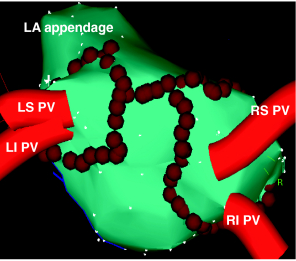
\includegraphics[scale=0.7]{./teile/introduction/ablation_cut.png}
\caption{Example of circumferential PV ablation. The ablation sites are indicated by the red dots. LI PV: Left inferior pulmonary veins, 
LS PV: left superior pulmonary veins, RI PV: right inferior pulmonary veins, RS PV: right superior pulmonary veins. Figure adapted 
from \cite{Ora06}}
\label{af_circ}
\end{center}
\end{figure}

\vspace*{-0.7cm}

Various ablation techniques exist, including the PV isolation by segmental ostial ablation, circumferential PV ablation (see 
fig. \ref{af_circ}), wide-area circumferential ablation and antral PV isolation \cite{Ora06, Ora03, Ouy04}. Antral PV isolation 
and wide-area circumferential ablation was shown to be effective for both patients with paroxysmal and persistent AF \cite{CE09, Ora03}. 
In a randomized study circumferential PV ablation was found to result in a sinus rhythm in 74\% of patients with chronic AF \cite{Ora06}. \newline

\newpage

The goal of PV ablation is to induce a complete electrical isolation of the PVs. This is verified by entrance and exit block during 
pacing at multiple sites within the PVs \cite{CE09}. Freedom from recurrent AF can be predicted by 
termination and noninducibility of AF during catheter ablation \cite{Ora02, Ora06, Hai05, Hai04, Ora04}. Termination 
of AF indicates elimination of all triggers and drivers of AF while noninducibility indicates the absence of residual trggers and drivers 
that may initiate and perpetuate AF \cite{CE09}. Termination is hence not a reliable predictor in patients with paroxysmal AF while 
noninducibility is likely to predict that the patients are going to stay in sinus rhythm (see figure \ref{freedom_recurrence}). 

\begin{figure}[H]
\begin{center}
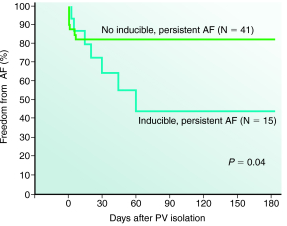
\includegraphics[scale=1]{./teile/introduction/freedom_recurrence_AF.png}
\caption{Graph showing freedom from AF reocurrence when patients had or had not inducible AF after circumferential PV isolation. Figure adapted 
from \cite{Ora04}}
\label{freedom_recurrence}
\end{center}
\end{figure}

% \newpage

\vspace*{-0.4cm}

Independent of the used procedure, anticoagulants like Warfarin are used in a diversity of patients. In order to establish international 
criteria for risk patients who should uptake anticoagulants, the CHADS$_{2}$-VASc score was defined \cite{ESC12} 
(\textbf{C}ongestive heart failure: 1 point, \textbf{H}ypertension: 1 point, {A}ge ($\geq$ 75): 2 points, \textbf{D}iabetes mellitus: 1 point, 
\textbf{S}troke: 2 points, \textbf{V}ascular disease: 1 point, \textbf{A}ge (65-74): 1 point, \textbf{S}ex (female): 1 point). 
Patients who obtain at least 2 point in the CHADS$_{2}$-VASc score are prescribed anticoagulants. Patients with 1 point might be prescribed 
anticoagulants, alternatively aspirin can be used. Patients with a score of 0 are supposed to only take aspirin \cite{Fle}. The 
CHADS$_{2}$-VASc score has been validated in multiple cohorts \cite{Lip11, Pot12, Ole12, Van11, Fri12, Ole11, Bor11}.


\newpage

\subsubsection*{Catheter ablation of AF: success rate and complications}

The FAST trial compared the outcome of catheter ablation and surgical ablation in a randomized study with a small patient population of 127 
patients. 63 patients were treated with catheter ablation, 64 with the invasive surgical ablation. 
The complication rate in catheter ablation was significantly lower (15.9\% complication rate in catheter ablation versus 34.4\% in surgical 
ablation) but at the same time the success rate in treatment outcome was reduced (36.5\% for catheter ablation versus 65.6\% for surgical 
ablation after 12 months) \cite{Boe12}. \newline

In two nationwide surveys the success rates of catheter ablation as a treatment for AF and the resulting complications were studied \cite{Cap05, Cap10}. 
The first worldwide multicenter survey was published in 2005 using data obtained from 181 centers in-between 1995 and 2002. 
From these centers 90 stated to have performed 12,830 catheter ablation procedures on 8,745 AF patients. 
It was stated that 52\% of AF patients undergoing ablation were symptom free without the need of further antiarrhythmic medication and 23.9\% 
of patients with the need of antiarrhythmic drugs. These success rates were achieved with the requirement of a 
a second (in 24.3\% of patients) or even third (in 3.1\% of patients) procedure \cite{Cap05}. Major complication rates were reported in 
6\% of patients. These complications included 4 early deaths (due to massive cerebral thromboembolism in two patients, extrapericardial PV 
perforation in one patient and unknown reasons in one patient), strokes (in 20 patients), transient ischemic attacks\footnote{"mini-stroke"; stroke-like symptoms due to loss of blood flow, no permanent damage} 
(in 47 patients) and episodes of tamponade\footnote{fluid collects between the heart muscle and the pericardium, which is the sac containing 
the heart} (in 107 patients). 
In a second survey which was performed in-between 2003 and 2006 \cite{Cap10} and included 85 catheter ablation 
performing centers (16,309 patients), an improvement in treatment outcome was shown. 
The rate for a successful treatment outcome without the need of further antiarrhythmic medication increased to 
70\% while the rate with the need of further antiarrhythmic medication decreased to 10\%, resulting in an overall success rate of 80\% 
compared to 75.5\% in the first survey. Concerning the number of needed procedures it was stated that 37.1\% single treatments were performed, 
59.8\% dual treatments and 4.1\% triple treatments.\newline

Recent studies furthermore show that catheter ablation procedures in AF patients are associated with a 
substantial risk of developing silent cerebral embolism \cite{Her13, Gai10, Marti13, Med13, Schr10, Lic06}. 
Silent cerebral embolism can cause cognitive impairment \cite{Kne08}. A study by Medi et al. \cite{Med13}, which investigated the 
post-operative neurocognitive dysfunction in 150 patients undergoing ablation before and after the treatment, stated a 13\% - 20\% incidence 
at long-term follow up of 3 months compared to a control group. \newline

Besides these major complications general disadvantages in the treatment modality of catheter ablation can be concluded. 
Procedures are tedious and can take up to five hours \cite{Jong05}. As fluoroscopy is still the mainstay of catheter imaging in most 
laboratories the patients are furthermore exposed to relatively high X-ray dose \cite{Ber10}. From an socio-economical point of view, 
catheter ablation causes high costs. A total of 13.5 billion Euro are spent on AF patients each year in the EU \cite{Fus06}.\newline

It can be concluded that catheter ablation offers only a limited treatment success rate while major complications and even death due to the 
procedure may occur. Alternative treatment modalities are warranted. Catheter-free ablation using carbon ions could have the potential to 
accurately eliminate arrythmogenic sources at any given cardiac location. So far conducted studies to irradiation of cardiac target sites will 
be presented in the next section. 


\subsubsection*{Heart irradiation and cardiac radiosurgery}
\label{cardiacradiosurgery}

Target sites in the heart have been irradiated in different procedures. Re-stenosis\footnote{reoccurrence of blood vessel narrowing} after 
angioplasty\footnote{mechanical widening of narrowed blood vessel e.g. with a balloon catheter} for example has been treated with vascular 
brachytherapy \cite{Nat99, Cot05}. Thereby a minimum dose of (8-16)Gy to a depth of 0.5mm into the vessel wall was required, while a 
maximum vessel dose did not exceed 32Gy. Cardiac angiosarcoma, a very rare tumor type in the heart with rare long-term 
survival of the patients, has been treated with carbon ions at the Japanese facility NIRS \cite{Aok04}. A total dose of 64Gy was given in 16 
fractions in a timeframe of 4 weeks. Follow-up of one and a half year did not show severe side effects.\newline
\newline
Similar to the techniques used in vascular brachytherapy, P\'erez-Castellano et al. \cite{Per06} studied the possibility to use $\beta$-radiation 
as treatment modality for AF. They thereby used a phosphorus-32 source wire centered within a balloon catheter in a study with ten mini swine. 
The delivered dose was calculated to 60Gy at a depth of 1 mm from the contacting PV wall, resulting in observed PV fibrosis without PV stenosis 
or other side-effects.\newline
\newline
In 2010 a study by Sharma et al. \cite{Sha10} showed that they were able to successfully alter the electrical pathway of the heart 
noninvasively by using stereotactic robotic radiosurgery. In the CyberHeart system cardiac target sites in sixteen mini swine were irradiated 
under general anesthesia. The procedure was as follows. Cardiac CT scans of the anesthetized and intubated mini swine were acquired and an 
electroanatomic mapping\footnote{CARTO system; Biosense-Webster. Three known magnetic sources are used to calculate the orientation 
and position of the catheter tip in 3D, while at the same time the voltage values are determined \cite{bw}} was carried out before the 
irradiation. The voltage was mapped to enable a comparison with the later to be induced electrophysiological effect. Different target sites 
in the heart were chosen. The respiratory motion was compensated by tracking with the CyberKnife Synchrony software, which correlates the 
outside motion of radiopaque markers on the chest wall with the internal motion 
\cite{Ozh08}. For the cardiac motion an ITV approach was chosen. Target volumes were the cavotricuspid isthmus (CTI) (nine mini swine), 
the AV node (two mini swine), the pulmonary vein - left atrial junction (three mini swine) and the left atrial appendage (two mini swine). 
Dose ranges from 25Gy to 80Gy were applied (cavotricuspid isthmus: (25-80)Gy, AV node: (40-70) days, PV: (38-40)Gy and left atrial 
appendage: (32-80)Gy). Post irradiation the mini swine were stored at a farm. The follow-up time was dependent on the irradiated target in 
the mini swine (cavotricuspid isthmus: 25 to 89 days, AV node: 15 to 49 days, PV: 35 to 196 days and left atrial appendage: 16 to 33 days). 
In order to assess the irradiation outcome, the animals were again anesthetized and electroanatomically mapped. Afterwards the mini swine 
were euthanized and targets (heart) as well as organs at risk (lung, esophagus) were excised and fixed in formaldehyde. The results of the 
irradiation can be summarized as follows:
The irradiation of the cavotricuspid isthmus evolved during the study, leading to changes in the method of targeting. While initially the 
respiratory and cardiac motion were not compensated for, synchrony and cardiac ITV concepts were later used. While all mini swine 
displayed a reduced conduction across the isthmus, only two animals showed bidirectional block and hence feasibility at 30 days and 40Gy.   
Targeting the AV node, one animal had to be sacrificed due to pacemaker pocket infection. The other one showed a complete AV block at 49 days, 
after being irradiated with 70Gy. For the left atrial appendage a decreased voltage was observed at 38Gy after 33 days. For the left 
pulmonary vein the feasibility was shown as the left atrium showed no local activation in all animals (present from day 35 for all doses) 
(see figure \ref{LA_map}).

\begin{figure}[H]
\begin{center}
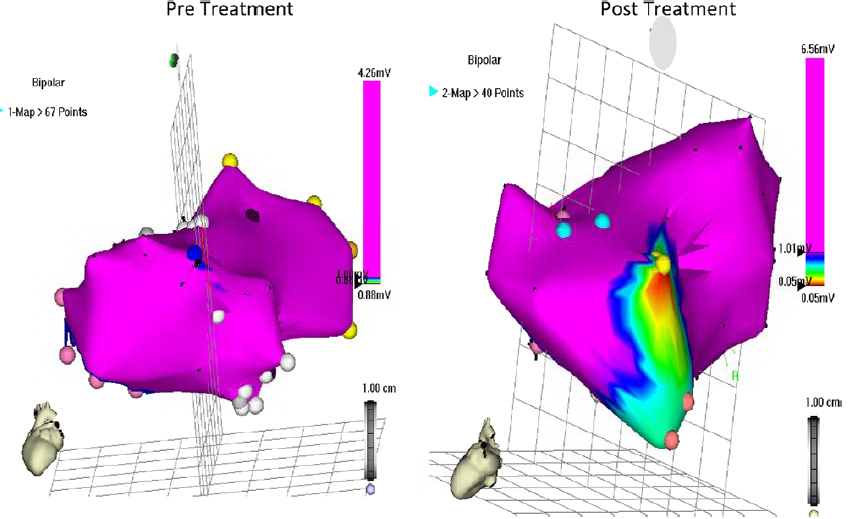
\includegraphics[scale=0.45]{./teile/introduction/cyberheart_voltagemap.png}
\caption{Electroanatomic voltage map of left atrium before (left side) and after (right side) CyberHeart irradation of PVs. Prior treatment 
no decreased voltage can be observed. Post treatment an area of low-amplitude action potential signals can be seen. Figure from \cite{Sha10}}
\label{LA_map}
\end{center}
\end{figure}

Sharma et al. stated that a dose of 25Gy or larger was needed to see a change in the electrophysiological properties in the animal model 
after 30 or more days. The dose needed for myocardial fibrosis is also known from other former studies. Fajardo et al. \cite{Faj70, Faj73} for 
example studied radiation induced fibrosis in rabbit hearts. They observed myocardial fibrosis most often after 2 to 70 days when irradiating 
the rabbits with 20Gy. Overall Sharma et al. proved that stereotactic radiosurgery has the potential to become a noninvasive treatment 
modality for e.g. atrial fibrillation. \newline

A subsequent study carried out with the CyberHeart system \cite{Mag11} only targeted the pulmonary veins atrial junction. Two mini swine 
were irradiated with a single fraction treatment of 25Gy and 35Gy, respectively and followed for 6 months. It was stated that both animals 
showed circumferential fibrosis, leading to an electrical isolation of the PVs, which was detected with an electroanatomic mapping. 
The mini swine irradiated with 35Gy showed more extensive necrosis and vasculitis in intramyocardial vessels. It was hence implied that 
25Gy are sufficient to induce a PV isolation with no major complications in the studied timespan. \newline

In an animal study carried out by Blanck et al. \cite{Bla13} 8 mini swine were irradiated with a single fraction of seven fields with doses 
between 17.5Gy and 35Gy. A 5D-ITV concept was applied, hence applying internal margins to the upper right PV accounting for the respiratory 
and heartbeat. Prior treatment electroanatomic mapping was carried out. The animals were followed for 6 months. In this study it was stated 
that a reduction of the electrical signal procession with correlating local transmural fibrosis in the target region was observed at 
doses above 30Gy. Nevertheless a complete block of the PVs could not be achieved. Stenosis in one branch of 
the PV was observed for the highest applied dose.\newline

All these studies were carried out with photon irradiation. Due to the physical and biological properties of carbon ions (see section \ref{pbb}) 
an improved outcome is expected when treating these deep seated target volumes while sparing the critical organs close by and exposing 
less volume of myocardium to low dose of radiation \cite{Ber12}. The feasibility of this treatment modalities with scanned carbon ions is the aim of 
the present work. 


                                                                                                                                                                                                                              
% \end{document}

  
  \setcounter{mtc}{2}
  
\chapter{Irradiation of pulmonary veins under influence of respiration in human data}
\label{chapter:mdacc}
\minitoc


PVs move due to the heartbeat and respiration of the patient. Both motion types are independent from each other and can hence be studied 
individually. While the influence of heartbeat is analyzed in chapter \ref{chapter:human}, the effect of respiratory motion will be discussed 
in this chapter. 4DCTs of nine lung cancer patients were recorded for cancer radiotherapy at MD Anderson Cancer Center in Houston (MDACC, 
Texas, USA) where patients were treated with proton therapy and IMRT. The same data has been used in previous studies on motion mitigation 
techniques using carbon ion beams (e.g. \cite{Lue12, Woe11}). The PV were contoured and the resulting motion pattern, direction as well as 
motion amplitude of LPV and RPV due to respiration were studied for all cases. Respiration is also a problematic factor for catheter ablation 
as it can cause changes in catheter contact force and hence alter the result \cite{Kum12}. For the proposed non-invasive treatment modality 
with a scanned carbon ion beam the respiratory motion will endanger the treatment outcome as it often leads to inhomogeneous dose coverage. Hence 
motion mitigation techniques are needed. The resulting interplay pattern for all patients as well as gating as a possible motion mitigation 
technique have been studied and the results will be presented in this chapter. Exemplary for two patient cases rescanning inside the gating 
window was analyzed. 

\section{Material and methods}
Details on the input data as well as the used treatment planning parameters will be given. Afterwards an overview on all 
studies will be presented and the analysis procedure will be described.  

\vspace*{-0.3cm}
\subsection{Treatment planning input data}
For treatment planning studies with the in-house treatment planning software TRiP4D \cite{Ric13}, 4DCT data sets, target and OAR contours as 
well as a deformable image registration for motion assessment in-between the different motion phases are needed. Details on the used 
input data as well as the used treatment planning parameters will be given.\newline 
\newline
In order to assess the motion of the PV due to respiration, lung cancer patient data was used. The 4DCTs of nine patients were recorded and 
anonymized at MDACC. Each of the 4DCT data consisted of ten motion phases, the reference phase was 
motion phase five at end exhale. The amplitude of the respiratory motion was assessed by measuring the difference between the (right) diaphragmatic dome in-between 
end exhale and end inhale on a frontal view of the 4DCT data. The amplitudes in the superior-inferior (SI) motion direction, the 
largest motion component in case of respiration, ranged from 2.5mm to 25mm (CT slice distance and hence resolution of 2.5mm). The varying 
motion amplitudes are displayed for all patients in 
table \ref{tab:patdata}. Two of the nine patients (patient 6 and 7) displayed a very shallow breathing with an amplitude of less than 5mm. 
Five patients (patient 1 to 5) had a breathing amplitude between 10mm and 20mm in SI direction. Two patients (patient 8 and 9) were breathing 
deeply with an amplitude bigger than 20mm. This indicates different breathing patterns as well as varying lung volume 
expansion and hence heart displacement amongst the studied patients. 

% \vspace*{-0.3cm}

\begin{table}[H]
  \centering
%   \footnotesize
  \caption{Respiratory motion in the direction of the largest motion component (SI) for all investigated patients. Furthermore the lung tumor 
  location (left lung (L) or right lung (R)) is stated next to the tumor volume.}
  \begin{tabular}{|c|c|c|c|}
    \hline\hline
    patient no & motion [mm] & tumor volume [cm$^{3}$] & tumor location (L/R)\\
    \hline
    1 & 17.5 & 236.5 & L \\
    2 & 20 & 572.2 & R \\
    3 & 10 & 160.2 & R \\
    4 & 17.5 & 676.1 & L \\
    5 & 15 & 372.1 & R \\
    6 & 2.5 & 706.1 & R \\
    7 & 5 & 123.8 & L \\
    8 & 25 & 44.7 & L \\
    9 & 22.5 & 125.3 & L \\
    \hline\hline
  \end{tabular}
  \label{tab:patdata}
\end{table}

\newpage

Segmentation of the LPV and RPV was performed with an in-house display functionality for TRiP \cite{Hil09}. Its graphical interface 
allows contouring on the axial slices of the reference phase of the 4DCT. The contours were checked and validated by a medical physicist 
who was involved in the animal studies of Sharma et al. \cite{Sha10} as well as a cardiologist from Mayo Clinic. Only the motion influence 
and the motion mitigation possibilities will be studied here, hence contouring of other volumes or organs at risk was omitted. A detailed 
analysis of the dose to the organs at risk in human data is performed in chapter \ref{chapter:human}. The volumes of the contours for the 
ablation sites for LPV and RPV are presented for each patient in table \ref{tab:volume}. 

\begin{table}[H]
  \centering
%   \footnotesize
  \caption{Target volume for LPV and RPV for all investigated patients.}
  \begin{tabular}{|c|c|c|}
    \hline\hline
    patient no & LPV [cm$^{3}$] & RPV [cm$^{3}$]\\
    \hline
    1 & 1.88 & 5.26 \\
    2 & 3.57 & 4.79 \\
    3 & 6.49 & 11.52 \\
    4 & 3.66 & 3.87 \\
    5 & 2.07 & 4.37 \\
    6 & 3.40 & 6.34 \\
    7 & 4.29 & 6.23 \\
    8 & 6.89 & 4.84 \\
    9 & 2.92 & 2.56 \\
    \hline\hline
  \end{tabular}
  \label{tab:volume}
\end{table}

Non-rigid image registration of the nine motion phases on the reference phase have been performed with Plastimatch \cite{Sharp07, Shack10}. 
A B-spline registration with the following parameters was chosen: The first step was carried out with 50 maximal iterations and an isotropic 
spacing of 35mm between the control points of the B-spline grid. In the second step, with 100 maximal iterations, the grid 
spacing was set to 11mm and the regularization to $\lambda$=0.005. 
The quality of registration was validated with visualization techniques: false color images \cite{Bro07}, checker board images 
\cite{Bro07} as well as a qualitative check of the vector field regularization. These tests were carried out between the two most extreme 
motion phases: the reference phase at end exhale (motion phase five) and the phase at end inhale (motion phase zero).


\subsection{Treatment planning parameters}
\label{mdacc:tpp}
Treatment plans without motion (3D, static) as well as with motion (4D) were generated. 
For the dose optimization process, 3D treatment plans were generated to homogeneously cover the CTVs in the reference phase while 4D treatment
plans covered the ITV \cite{Gra12}, which was generated from all twenty motion phases. 
Besides the original volume of the CTV safety margins have been added to the volumes of the treatment planning study. These margins were applied 
in order to account for possible deviations in between treatment planning and delivery, like positioning errors, changes 
between CT acquisition and treatment delivery etc. Isotropic safety margins of 3mm, 5mm and 7mm have been chosen. The ITV volumes used as the 
final PTV target were generated from the original CTV contour as well as the CTVs with margin, so that potential range variations were 
considered in the margins.\newline
\newline
The grid spacing was chosen to be 1$\mathrm{mm}$, both in $x$ and $y$ direction. The spacing between the IESs were chosen to be 3 mm$_{H2O}$. 
A maximal contour extension\footnote{determines the extent of rasterpoint positions outside the target contour} of 1.1 times the focal 
spot size of 4mm was chosen as well as a distal contour fall off of 4mm$_{H2O}$. TRiP's 'all points divergent beam' algorithm was used to 
calculate the absorbed dose. All treatment plans were calculated as intensity modulated particle therapy (IMPT). 
Following Sharma et al. \cite{Sha10} a physical dose of 25Gy was applied in one fraction in all simulations.\newline
\newline
Three different beam entrance directions were used. For all beam directions the couch was rotated by 90$^{\circ}$ while the 
gantry angles were set to -45$^{\circ}$, 135$^{\circ}$ and 0$^{\circ}$, respectively. With these field number and directions a good sparing 
of normal tissue, especially of the coronary arteries as well as of the aorta and of the trachea could be obtained (see chapter \ref{chapter:human}). 
The field directions were validated by a cardiologist from Mayo Clinic.\newline
\newline
The generation of treatment plans is furthermore also dependent on the theoretically possible 
beam application. Spill length, shape and particle intensity are thus important factors. For the here presented simulations HIT accelerator 
parameters have been used. Thereby a spill length of up to 5s is assumed. The pause in between spills has a mean value of 4.5s. The spill 
shape is rectangular. The particle intensities at HIT used for treatment planning vary between 5x10$^{6}$ and 8x10$^{7}$ particles per spill. 
Inbetween these two extreme intensity levels, eight different intensity levels can be used. In the resulting treatment plan, the intensity 
steps are automatically chosen \cite{Krae00, Ric13}. The minimum particle number per beam spot was set to 11,000.\newline
\newline
As the reconstruction of the 4DCTs was based on the time scale a phase-based motion state detection was employed. 
A Lujan motion type was chosen for the motion trajectories \cite{Luj99}. In order to consider possible divergence in the respiratory motion 
pattern of patients, different periods (6s and 8s) as well as different starting phases (0$^{\circ}$ and 90$^{\circ}$) were used. 
The motion periods were chosen according to the respiratory rate of 8 to 10 cycles per minute. 

\newpage

\subsection{Treatment planning studies}

3D treatment plans on the CTV volume were produced as reference values to the 4D cases, as it represents the ideal but not deliverable dose 
distribution. Different ITV margins (original and increased with 3mm, 5mm and 7mm margin) were studied for all patients in the 4D treatment plans. 
In order to prepare for these 4D simulations, the motion of the PVs due to respiration was assessed. 
4D plans were distinguished between an underlying motion without any compensation, resulting in interplay patterns \cite{Phi92, Ber08}, 
and with the application of gating \cite{Kub96} as motion mitigation technique. The gating window was set to 30\% around end exhale (reference 
phase five), so that motion phases four, five and six were used. For two patient cases (patient 2 and 9) rescanning inside the gating window 
was furthermore studied. Thereby four different rescan numbers (five, ten, fifteen and twenty rescans) have been studied. Treatment plans for 
all patients where carried out with one beam channel combination (couch angle of 90$^{\circ}$ and gantry angles of -45$^{\circ}$, 
135$^{\circ}$ and 0$^{\circ}$), all four safety margins, the stated treatment planning parameters and the four stated motion trajectories. 


\subsection{Analysis}

For comparison of the resulting dose coverage dose-volume-histograms (DVHs) were studied. The V95 (measure of dose coverage) and V107 (measure 
of over dosage) of the CTVs were analyzed. As an indicator for the dose homogeneity, the width of the dose fall off was determined by analyzing 
the difference D5-D95. The stated values have been evaluated for all beam application techniques (static, interplay, gating, rescanning within 
gating window). Furthermore motion-volume-histograms (MVHs) were generated in order to assess the resulting motion of the PV due to respiration. \newline
\newline
In order to study correlations between the diaphragm motion and the motion of the PVs the Pearson coefficient $r$ was determined and 
is reported for limits of $p$<0.05. Furthermore the relation of dose analysis parameters to different margin sizes and the studied irradiation 
technique was analyzed by a one-way analysis of variance (one-way ANOVA) and the proportion of variance explained ($r^{2}$ - which ranges from 
zero (fit has no predictive value) to one) and is reported with the corresponding p-value ($p$<0.0001). \newline
\newline
Boxplots of dose analysis parameters D5-D95 and V95 over all patient data sets, motion patterns and target volumes were moreover generated 
in order to study the influence of margin size and irradiation mode (static, interplay and gating). Thereby the median (50th 
percentile) as well as the 25th and 75th percentile are displayed next to the minimum and maximum. 
 

\newpage

\section{Results}

In the following the results of the motion assessment as well as of the treatment planning studies for all studied cases 
(static, interplay and gating as well as rescanning within the gating window) will be presented.  
The expected treatment time will be discussed. 


\subsection{Motion assessment of respiration}
\label{motion}
Using the resulting deformation maps from deformable image registration the motion of the ablation sites of LPV and RPV was assessed. Motion 
volume histograms (MVHs) \cite{Ric13} displaying the relative displacement of every voxel of the investigated volume to the reference phase 
in all three motion directions (SI: superior-inferior, AP: anterior-posterior, LR: left-right) as well as the absolute displacement (ABS) 
were generated. The mean and standard deviation of these displacement values in each motion phase of LPV and RPV are plotted for all patients 
and motion directions in figure \ref{motion_resp_all_lpv} and \ref{motion_resp_all_rpv}, respectively. The numerical values can be found 
in appendix \ref{app:mdacc:motion}. \newline
\newline
The mean and standard deviation of the displacement between the two extreme motion phases (end exhale and end inhale) are shown for all 
patients in tables \ref{tab:motion:LPV:mdacc} and \ref{tab:motion:RPV:mdacc} for the different motion directions and for the two target volumes, LPV and 
RPV, respectively. 
Depending on the patient the absolute displacement of the pulmonary veins were found to vary between three millimeters and more than 
one centimeter. From the nine studied patients patient 9 is displaying the highest absolute displacement, both in LPV and RPV.
For all patients, the largest motion direction is SI, resulting in the largest contribution to the absolute displacement. The 
average in SI direction over the entire volume reaches up to 15.5mm (average over all patients of (6.8 $\pm$ 3.8)mm) for LPV and 10.9mm 
(average over all patients of (6.8 $\pm$ 2.5)mm) for RPV. The other two motion directions show a much smaller displacement. In AP direction the maximal 
motion is less than 2.5mm (standard deviation of less than 1mm) and in LR the PVs move less than 2.7mm (standard deviation of 1mm).
Over all patients, the mean absolute displacement in-between end exhale and end inhale of the LPV is (6.8 $\pm$ 3.6)mm and 
(6.8 $\pm$ 2.5)mm for RPV. For the SI direction, the mean displacement over all patients is (-6.4 $\pm$ 3.8)mm for LPV and (-6.6 $\pm$ 2.4)mm for 
RPV.\newline
\newline
It can furthermore be seen that the relative displacement of the target volumes around end exhale (motion phase five, reference phase) is small 
for all motion directions and patients. The difference between motion phase four and six was only 3mm in the absolute displacement 
of patient 9, which is the patient with the largest motion in the patient cohort. Hence gating around end exhale was expected to be an 
adequate motion mitigation technique for the irradiation of the PVs under influence of respiration. 


%%%%%%%%%%% MVHs %%%%%%%%%%%%%%%%

\newpage

\begin{figure}[H]
\begin{center}
 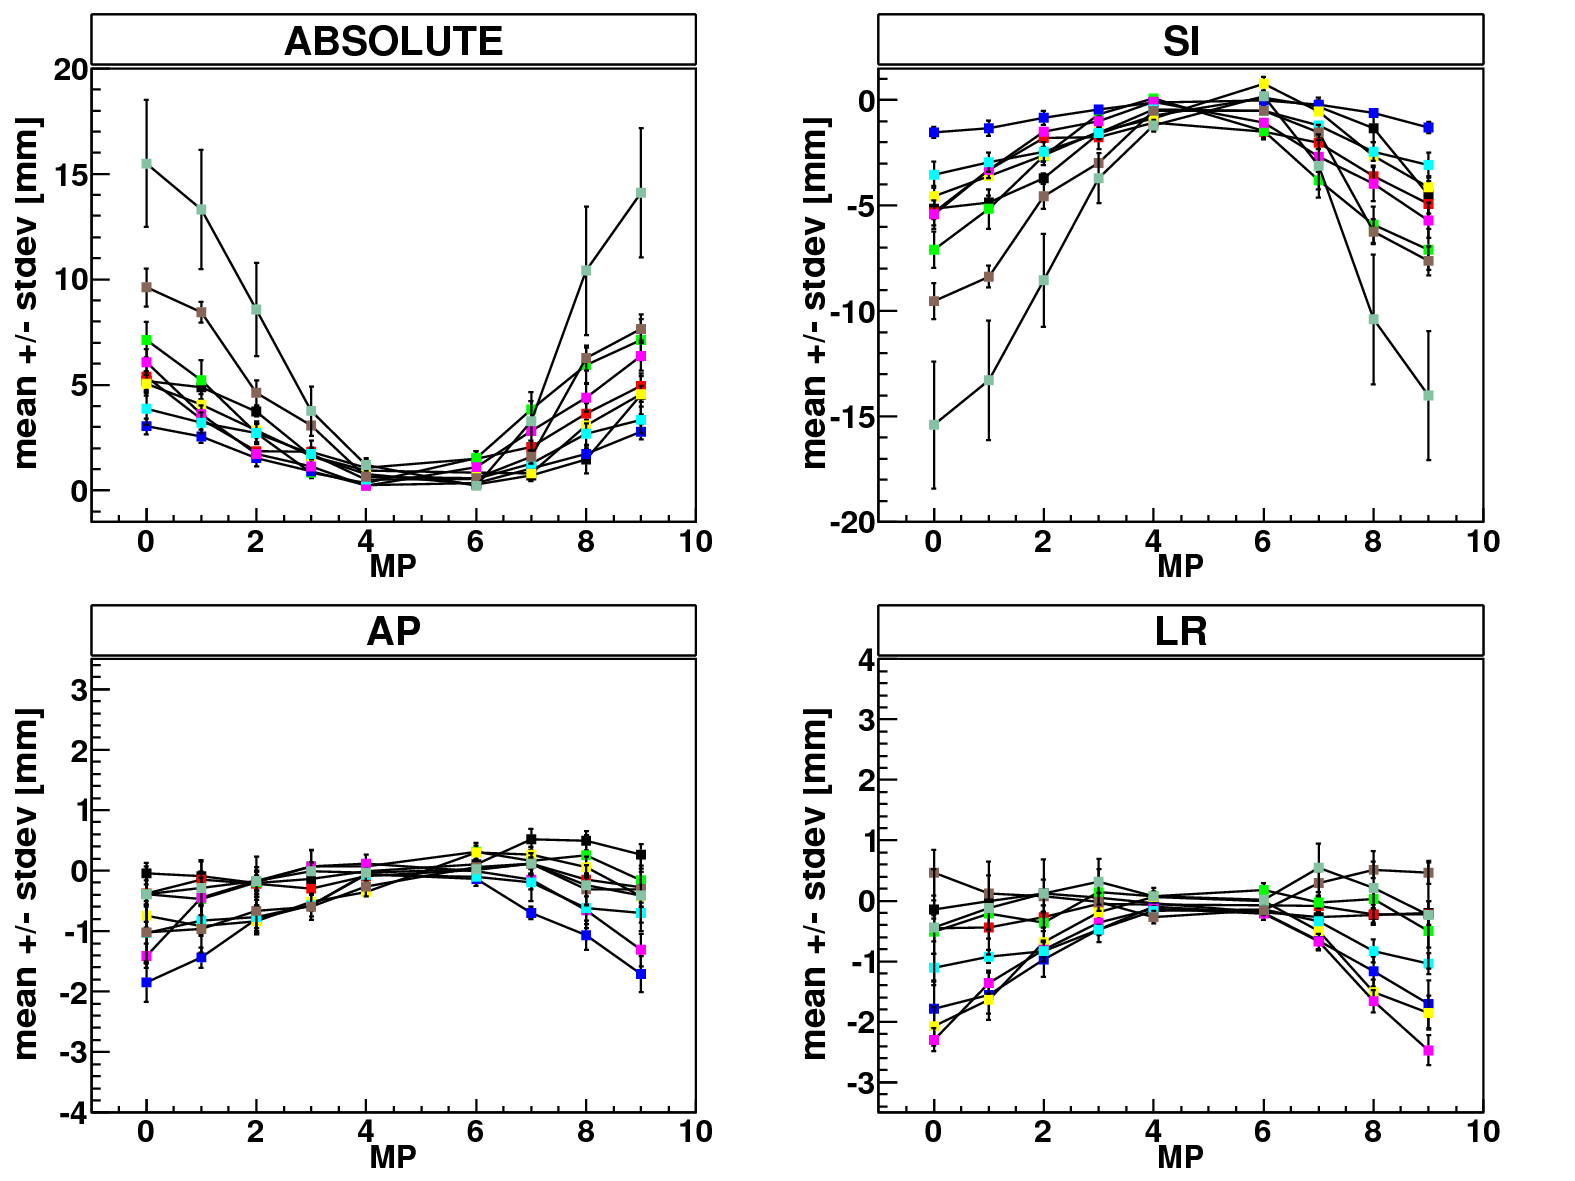
\includegraphics[scale=0.22]{./teile/results_mdacc/MDACC_allPatients_RESP_LPV.png}
\caption{LPV: Mean motion amplitude and standard deviation in each motion phase (MP) relative to the reference phase under influence of 
respiration for all patients (patient 1: black, patient 2: red, patient 3: green, patient 4: blue, patient 5: yellow, patient 6: pink, patient 
7: turquois, patient 8: brown, patient 9: olive). }
\label{motion_resp_all_lpv}
\end{center}
\end{figure}

\vspace*{-1cm}

\begin{figure}[H]
\begin{center}
 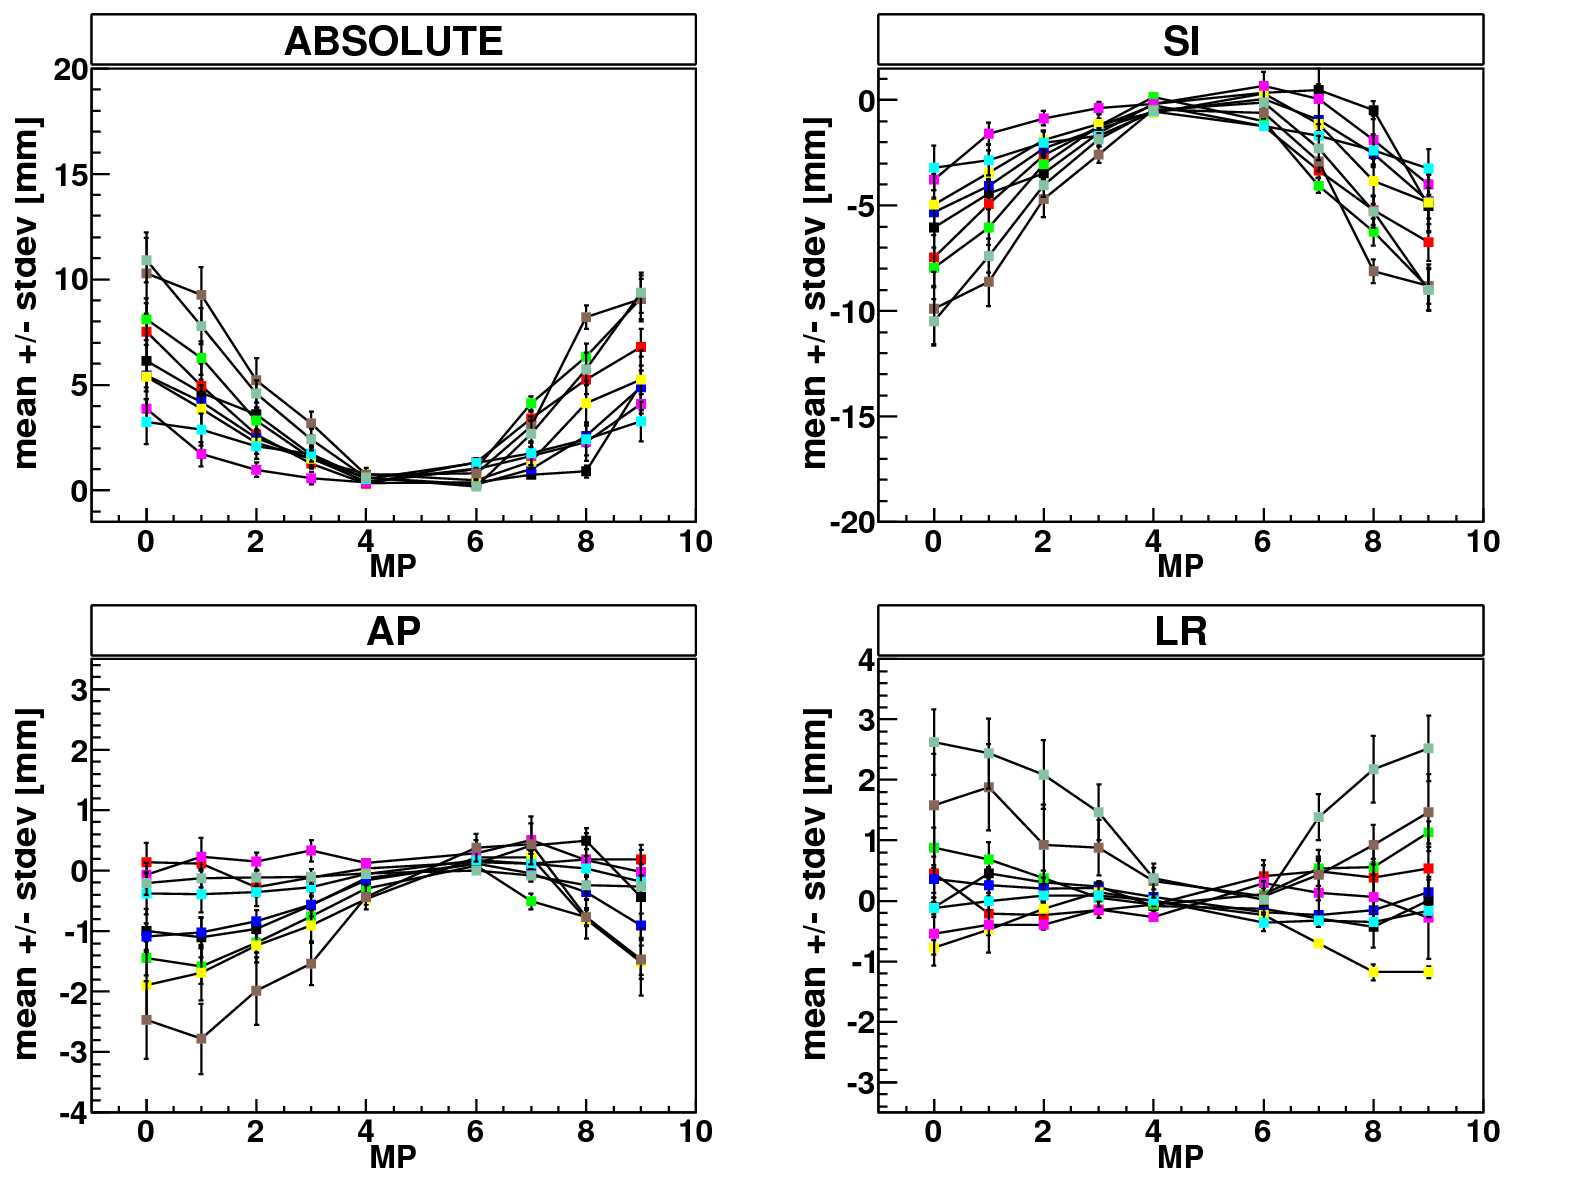
\includegraphics[scale=0.22]{./teile/results_mdacc/MDACC_allPatients_RESP_RPV.png}
\caption{RPV: Mean motion amplitude and standard deviation in each motion phase (MP) relative to the reference phase under influence of 
respiration for all patients (patient 1: black, patient 2: red, patient 3: green, patient 4: blue, patient 5: yellow, patient 6: pink, patient 
7: turquois, patient 8: brown, patient 9: olive). }
\label{motion_resp_all_rpv}
\end{center}
\end{figure}

\newpage

\begin{table}[htbp]
  \centering
  \caption{LPV: Mean and standard deviation of target motion in-between end exhale (motion phase five) and inhale (motion phase zero) for 
  all investigated patients.}
  \begin{tabular}{|c|c|c|c|c|}
    \hline\hline
    patient no & ABS [mm] & SI [mm] & AP [mm] & LR [mm]\\
    \hline
    1 & 5.2 $\pm$ 0.5 & -5.2 $\pm$ 0.5 & -0.1 $\pm$ 0.2 & -0.1 $\pm$ 0.2 \\
    2 & 5.3 $\pm$ 0.6 & -5.3 $\pm$ 0.6 & -0.4 $\pm$ 0.2 & -0.5 $\pm$ 0.2 \\
    3 & 7.1 $\pm$ 0.9 & -7.1 $\pm$ 0.9 & -0.4 $\pm$ 0.4 & -0.5 $\pm$ 0.4 \\
    4 & 3.0 $\pm$ 0.4 & -1.5 $\pm$ 0.3 & -1.9 $\pm$ 0.3 & -1.8 $\pm$ 0.5 \\
    5 & 5.1 $\pm$ 0.6 & -4.6 $\pm$ 0.5 & -0.8 $\pm$ 0.2 & -2.1 $\pm$ 0.3 \\
    6 & 6.1 $\pm$ 0.6 & -5.4 $\pm$ 0.7 & -1.4 $\pm$ 0.2 & -2.3 $\pm$ 0.2 \\
    7 & 3.9 $\pm$ 0.8 & -3.6 $\pm$ 0.6 & -1.0 $\pm$ 0.4 & -1.1 $\pm$ 0.2 \\
    8 & 9.6 $\pm$ 0.9 & -9.5 $\pm$ 0.9 & -1.0 $\pm$ 0.5 & 0.5 $\pm$ 0.4 \\
    9 & 15.5 $\pm$ 3.0 & -15.4 $\pm$ 3.0 & -0.4 $\pm$ 0.5 & -0.4 $\pm$ 1.0 \\
    \hline\hline
  \end{tabular}
  \label{tab:motion:LPV:mdacc}
\end{table}

\vspace*{-0.5cm}

\begin{table}[htbp]
  \centering
  \caption{RPV: Mean and standard deviation of target motion in-between end exhale (motion phase five) and inhale (motion phase zero) for all 
  investigated patients.}
  \begin{tabular}{|c|c|c|c|c|}
    \hline\hline
    patient no\rule{0pt}{2.6ex}\rule[-1.2ex]{0pt}{0pt} & ABS [mm] & SI [mm] & AP [mm] & LR [mm]\\
    \hline
    1 & 6.1 $\pm$ 1.4 & -6.0 $\pm$ 1.4 & -1.00 $\pm$ 0.4 & -0.1 $\pm$ 0.2 \\
    2 & 7.5 $\pm$ 1.4 & -7.5 $\pm$ 1.4 & 0.1 $\pm$ 0.3 & 0.5 $\pm$ 0.4 \\
    3 & 8.1 $\pm$ 1.0 & -7.9 $\pm$ 1.0 & -1.5 $\pm$ 0.4 & 0.9 $\pm$ 0.3 \\
    4 & 5.5 $\pm$ 0.6 & -5.3 $\pm$ 0.6 & -1.1 $\pm$ 0.2 & 0.4 $\pm$ 0.2 \\
    5 & 5.4 $\pm$ 1.5 & -5.0 $\pm$ 1.4 & -1.9 $\pm$ 0.6 & -0.8 $\pm$ 0.1 \\
    6 & 3.9 $\pm$ 0.5 & -3.8 $\pm$ 0.5 & -0.1 $\pm$ 0.2 & -0.6 $\pm$ 0.5 \\
    7 & 3.3 $\pm$ 1.1 & -3.2 $\pm$ 1.1 & -0.4 $\pm$ 0.3 & -0.1 $\pm$ 0.1 \\
    8 & 10.3 $\pm$ 1.9 & -9.9 $\pm$ 1.7 & -2.5 $\pm$ 0.6 & 1.6 $\pm$ 0.9 \\
    9 & 10.9 $\pm$ 1.1 & -10.5 $\pm$ 1.1 & -0.2 $\pm$ 0.2 & 2.6 $\pm$ 0.5 \\
    \hline\hline
  \end{tabular}
  \label{tab:motion:RPV:mdacc}
\end{table}

\vspace*{-0.5cm}

Possible correlations between the underlying respiration amplitude (see table \ref{tab:patdata}) and the displacement of the ablation sites 
for the PVs have been studied. It can be stated that in AP and LR direction, no correlation was observed. In case of SI displacement the 
results varied depending on the target volume. While no correlation was observed between the diaphragma motion and the SI displacement of the 
LPV ablation, the site for RPV showed a strong linear relationship (r=0.73, p<0.05). This resulted in a strong correlation between  
diaphragm motion and the absolute displacement of the RPV ablation site (r=0.79, p<0.05). For the LPV again no correlation was observed in the 
absolute displacement. \newline
\newline
It should be noted that these findings are based on a small number of lung cancer patients (see table \ref{tab:patdata}), which can alter the 
breathing pattern and heart motion and hence the result. It is unclear whether atrial fibrillation patients would display the same motion 
dependence and correlation results, though the result was independent of the tumor position in the left or right lung. 
\newpage
The overall displacement field between the two extreme states, end exhale and end inhale, for two exemplary patients with a small motion 
amplitude (patient 7) and a large motion amplitude (patient 9) are shown in figure \ref{contour_pat036} and \ref{contour_pat122}. In order to 
visualize the location of the displacement, an axial cut of the reference state CT is underlayed. The absolute values of the displacement 
vectors are shown as contour plots. 

\begin{figure}[H]
\begin{center}
 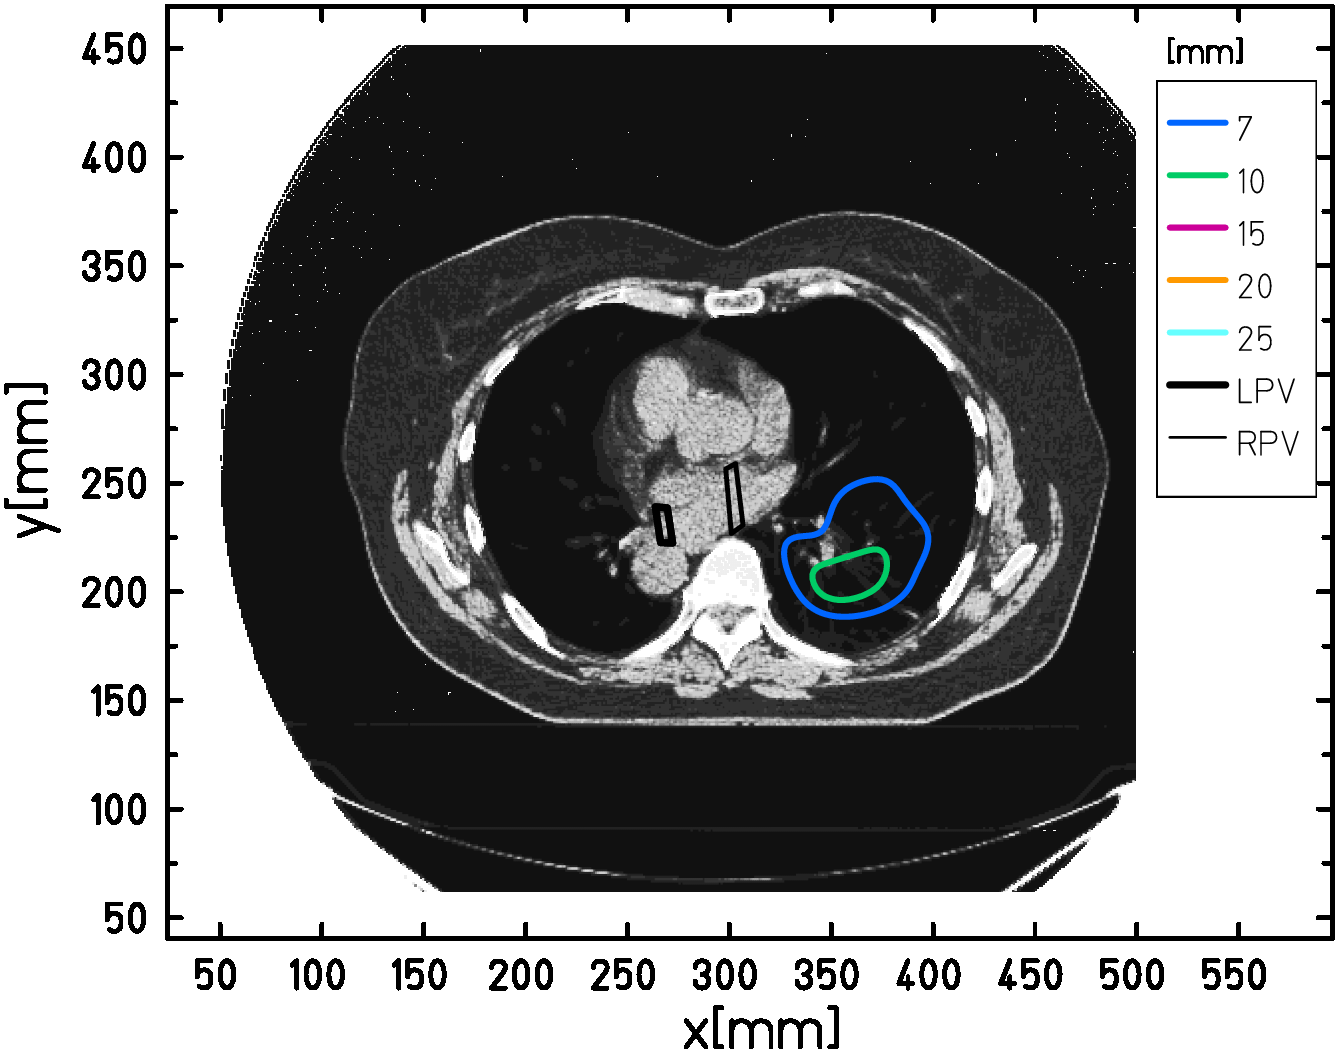
\includegraphics[scale=0.22]{./teile/results_mdacc/Contour_z_abs_RESP_Pat037_HUSkala_gedreht_2.png}
\caption{Contour plot of Patient 7}
\label{contour_pat036}
\end{center}
\end{figure}

\vspace*{-0.3cm}

\begin{figure}[H]
\begin{center}
 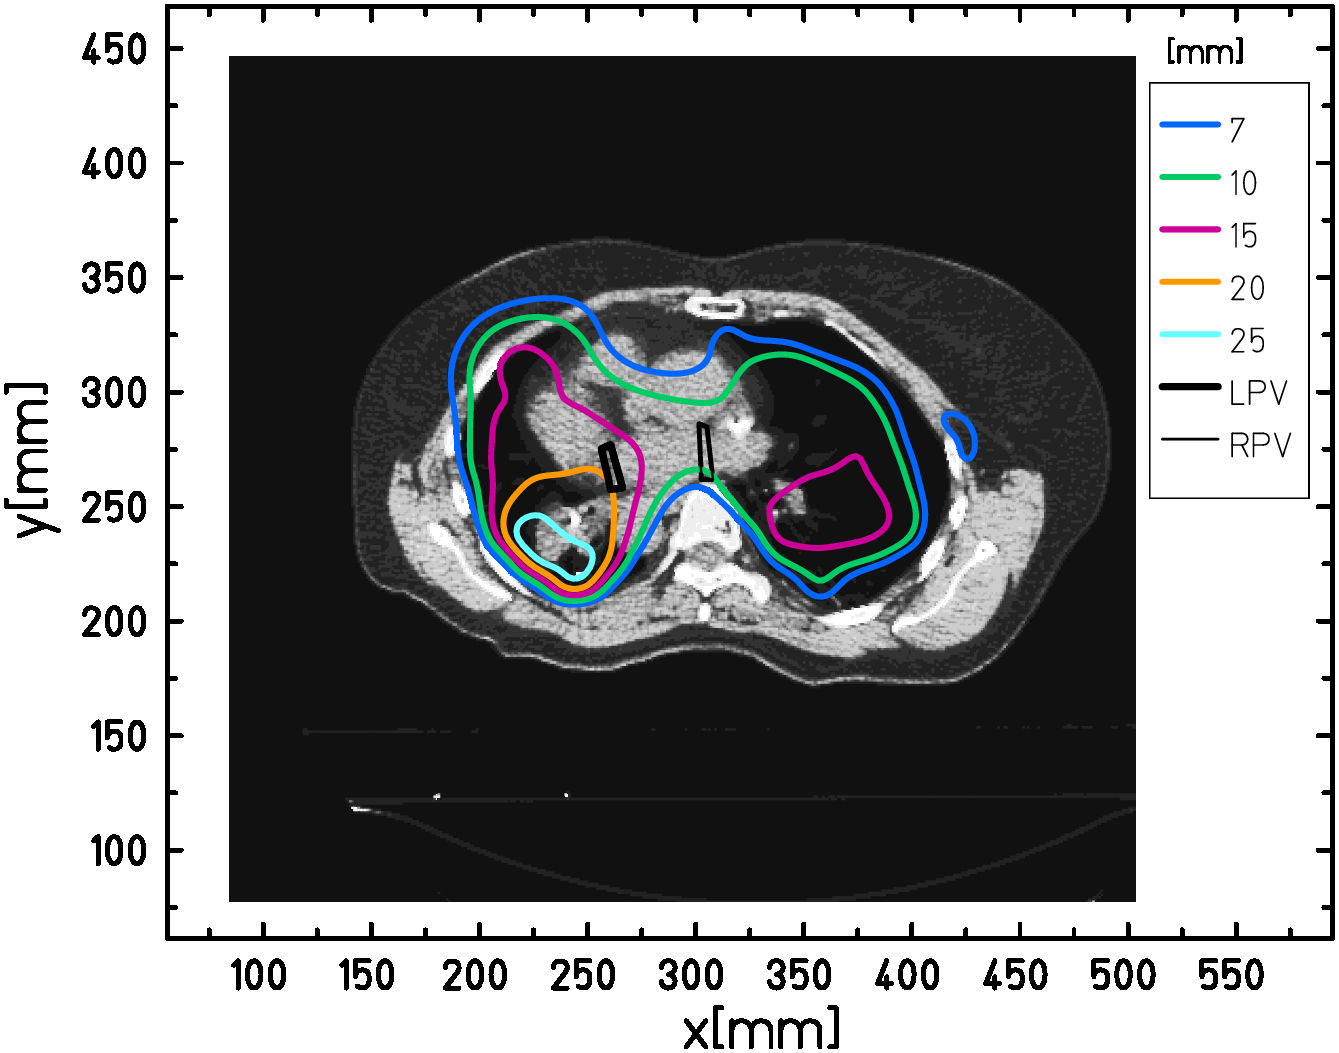
\includegraphics[scale=0.22]{./teile/results_mdacc/Contour_z_abs_RESP_Pat122_HUSkala_gedreht_2.png}
\caption{Contour plot of Patient 9 }
\label{contour_pat122}
\end{center}
\end{figure}

\newpage


\subsection{Motion mitigation techniques for respiration}
\label{mmt}
The absolute motion amplitudes of up to 1cm due to respiration are expected to yield dose inhomogeneity when not compensated for. The 
resulting interplay effect and dose deposition were studied for every patient for different motion patterns and different margins to the target 
volumes. The dose analysis values V95, V107 and D5-D95 were assessed and plotted. For comparison also the corresponding 
values for the 3D case (static) are shown. As shown in section \ref{motion} the motion displacement in the motion phases around 
end exhale (motion phase four to motion phase six) are rather small in all patient cases. Hence gating has the potential to be a 
well-suited motion mitigation technique to overcome the influence of target volume motion due to respiration. The results of the stated dose 
values in case of gating on the stated phases will be presented. 


\subsubsection{Dose deposition}

A representative dose deposition for all studied techniques (static, interplay and gating) is shown exemplary for patient 9 (as this is the 
patient with the largest PV motion amplitude) in figure \ref{dose_pat122}. Gating and interplay are shown for a motion period of 6s 
and a starting phase of 0$^{\circ}$. The target volumes LPV and RPV were irradiated simultaneously and a margin of 3mm was added. It can 
already been seen from these dose cut figures that gating around end expiration drastically improves the outcome compared to interplay and yields 
a result which is comparable to the static case.\newline
\newline
In order to assess the dose information for the whole volume the DVHs (see figure \ref{dvhs_pat09_mdacc}) of all patients were analyzed and compared for dose homogeneity, 
dose coverage as well as over dosage. The average results over all patients with the resulting standard deviation can be seen in 
figure \ref{static_interplay_gating}. A more detailed analysis can be found in appendix \ref{app:mdacc}, where the corresponding numerical 
values are shown (tables \ref{tab:Pat01:LPV} - \ref{tab:Pat09:RPV}) .\newline
\newline
For interplay it can be seen that the results are dependent on the used motion period and starting phase. This can be seen in the 
mean values of the resulting dose parameter values for different underlying motion patterns. E.g. for LPV, the mean value of the dose 
coverage parameter over all patients is V95=(90.3 $\pm$ 4.3)\% for a motion with 6s period and a starting phase of 90$^{\circ}$ and 
(89.3 $\pm$ 5.5)\% for a motion period of 8s and starting phase of 90$^{\circ}$, while for a motion period of 8s 
and a starting phase of 0$^{\circ}$ the dose coverage is (87.1 $\pm$ 7.8)\%. 
The safety margin influences the treatment outcome, as e.g. the dose coverage for a motion with 6s period 
and a starting phase of 90$^{\circ}$ has a mean value of (94.2 $\pm$ 4.8)\% with 3mm safety margin. All these dependencies are also valid for 
the other studied dose analysis parameters, dose homogeneity and over dosage. The improvement of the dose coverage and dose homogeneity 
in relation to the size of the safety margin are also presented in figure \ref{static_interplay_gating_ALLpatients_KORR} (a and b). 
The explained variance of the dose homogeneity versus the studied safety margins resulted in $r^{2}$=0.30 (p<0.0001).\newline 
\newline
The underlying deformation map with its motion amplitude enables a prediction of the magnitude of the interplay effect. 
This was studied in more detail for the dose homogeneity, as these values were normally distributed. 
The explained variance of the maximal motion amplitude of the left and right PV (see table \ref{tab:motion:LPV:mdacc} and 
\ref{tab:motion:RPV:mdacc}) and the resulting D5-D95 values for all studied margins was $r^{2}$=0.25 (p<0.0001).\newline 
\newline
Gating yielded improved results compared to interplay in all studied cases (see also figure \ref{static_interplay_gating_ALLpatients_KORR}). 
This is valid for dose homogeneity, dose coverage as 
well as over dosage. Especially dose coverage and over dosage are comparable to the static results for all patient and motion patterns 
(e.g. patient 1, V95 of 100\% for all studied motion patterns and safety margins in RPV, see table \ref{tab:Pat01:RPV}). In some patients the 
dose coverage is better with added safety margins (e.g. patient 9, V95 with no margin for motion period of 6s and starting phase of 0$^{\circ}$ is 94.1\% for LPV, 
a V95 of 99.9\% can be achieved for the same motion pattern with a margin of 3mm). Also in dose homogeneity a bigger safety margin tends to 
improve results (e.g. in LPV of patient 1 with motion period of 8s with starting phase of 0$^{\circ}$: D5-D95 = 4.4\% with margin of 3mm 
versus D5-D95 = 3.8\% with margin of 5mm). These findings are also shown in figure \ref{static_interplay_gating_ALLpatients_KORR}. Here 
the dose coverage and dose homogeneity are shown for all patients, motion patterns and the two target sites (LPV and RPV) depending on the 
used safety margin. It can be seen that the dose coverage is already drastically improved with 3mm margin. Also the dose homogeneity is 
improved with increasing safety margin. 
The explained variance of D5-D95 versus all studied margins resulted in $r^{2}$=0.40 (p<0.0001). 
Keeping the safety margin constant, it was nevertheless found that in some cases 
the dose homogeneity is not drastically improved by gating compared to interplay. The LPV of patient 2 for example 
has a D5-D95 value of 6.8\% for gating with a safety margin of 3mm (motion period of 6s and starting phase of 90$^{\circ}$), which is 
only slightly under the interplay result of D5-D95=8.4\% for the same safety margin and motion. However, the dose homogeneity value of 
interplay in this particular patient case is already lower than in other cases (e.g. D5-D95=10.6\% in patient 1 or 20.93\% in patient 9 
for 3mm margin and a motion period of 6s, starting phase of 90$^{\circ}$).\newline
\newline
As a method to further improve the dose homogeneity rescanning inside the gating window was studied for two patient cases. The results are 
presented in the next section. It can nevertheless be concluded that gating of target volumes with safety margin yields results comparable to 
the static irradiation in case of under and overdosage and hence is an adequate motion mitigation technique for the irradition of the 
PVs under influence of respiration. 



\newpage

 \begin{figure}[H]
 \begin{center}
\subfigure[static]{
 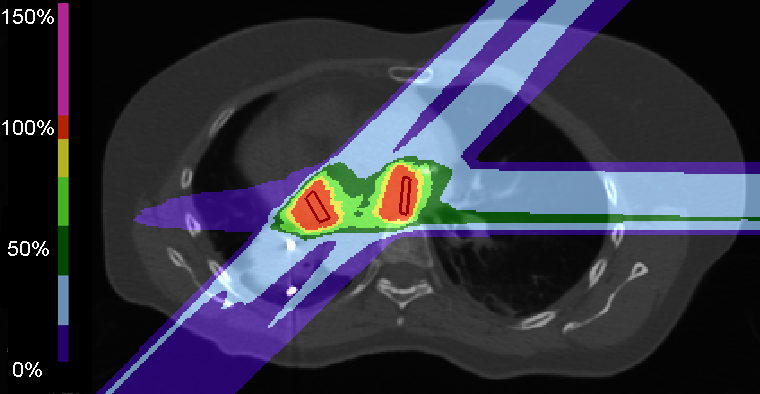
\includegraphics[scale=0.6]{./teile/results_mdacc/Pat122_slice50_static.png}
 }
\subfigure[interplay]{
 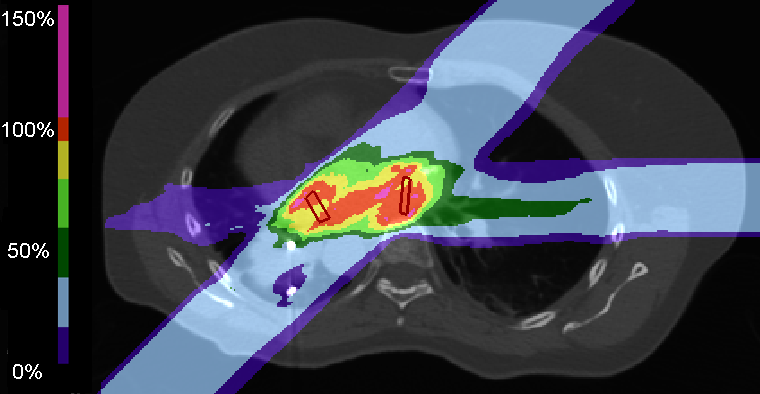
\includegraphics[scale=0.6]{./teile/results_mdacc/Pat122_slice50_interplay.png}
 }
 \subfigure[gating]{
 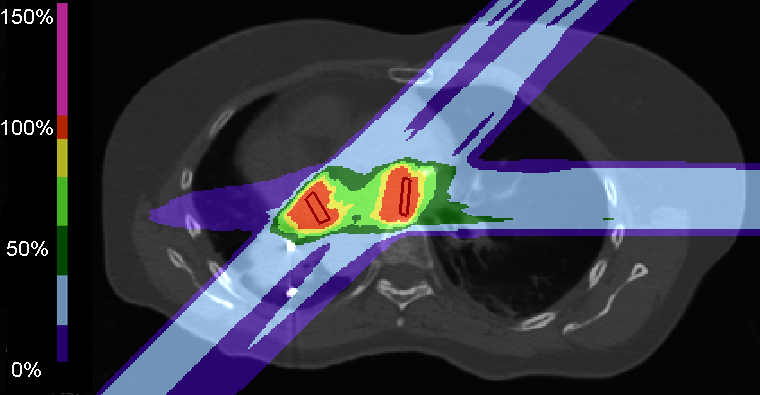
\includegraphics[scale=0.6]{./teile/results_mdacc/Pat122_slice50_gating.png}
 }
\caption{Dose distribution of patient 9 for static (a) as well as interplay (b) and gating (c) at motion period of 6s and a motion starting 
phase of 0$^{\circ}$. The target volume has an added margin of 3mm. The improved outcome of gating compared to interplay 
can already be seen in these dose cuts.}
\label{dose_pat122}
 \end{center}
\end{figure}

\newpage


 \begin{figure}[H]
 \begin{center}
\subfigure[LPV]{
 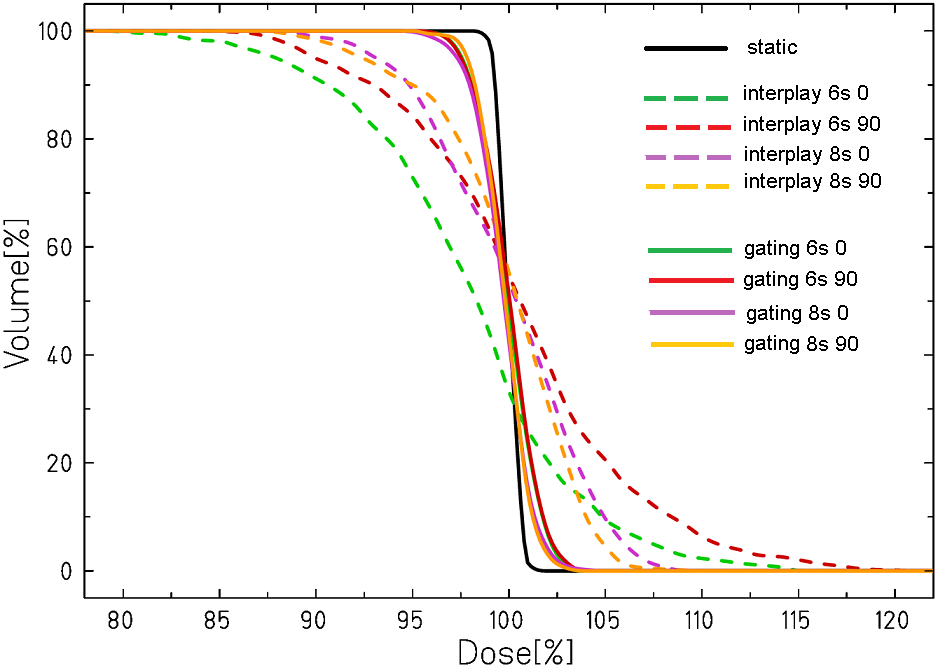
\includegraphics[scale=0.48]{./teile/results_mdacc/Pat09_allDVHs_LPV_withLegend.png}
 }
\subfigure[RPV]{
 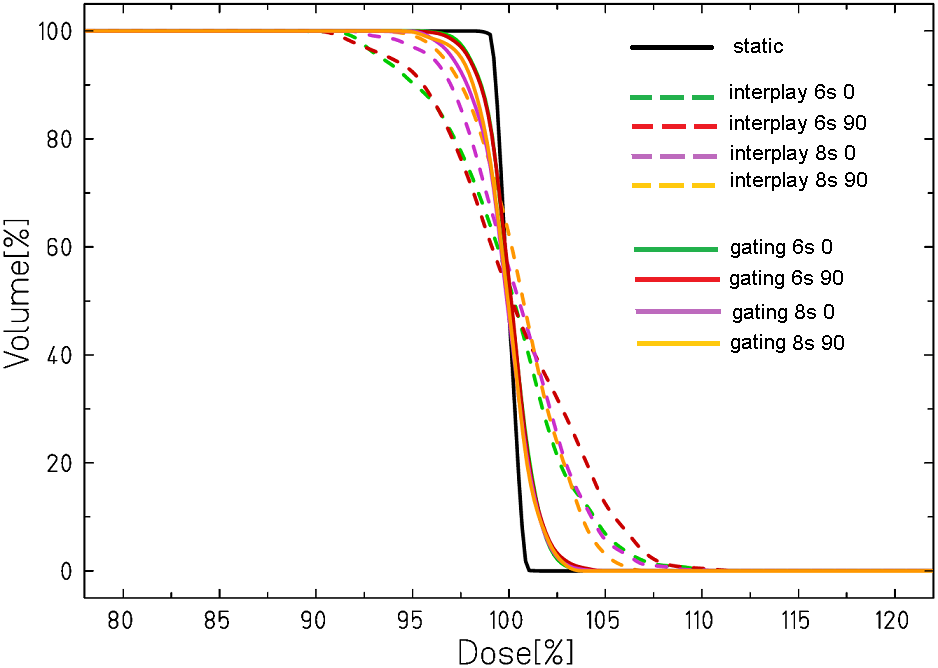
\includegraphics[scale=0.48]{./teile/results_mdacc/Pat09_allDVHs_RPV_withLegend.png}
 }
\caption{Dose volume histograms for CTV of patient 9 for 3mm safety margin irradiation (LPV (a) as well as RPV (b)) in case of static 
irradiation (black), interplay (dashed) and gating (solid). The motion patterns are shown in colors (6s 0: lujan motion with period of 6s 
and starting phase 0$^{\circ}$, 6s 90: lujan motion period of 6s and starting phase 90$^{\circ}$, 8s 0: lujan motion period of 8s 
and starting phase 0$^{\circ}$, 8s 90: lujan motion period of 8s and starting phase 90$^{\circ}$.}
\label{dvhs_pat09_mdacc}
 \end{center}
\end{figure}

\newpage

\begin{figure}[H]
\subfigure[D5-D95: LPV]{
 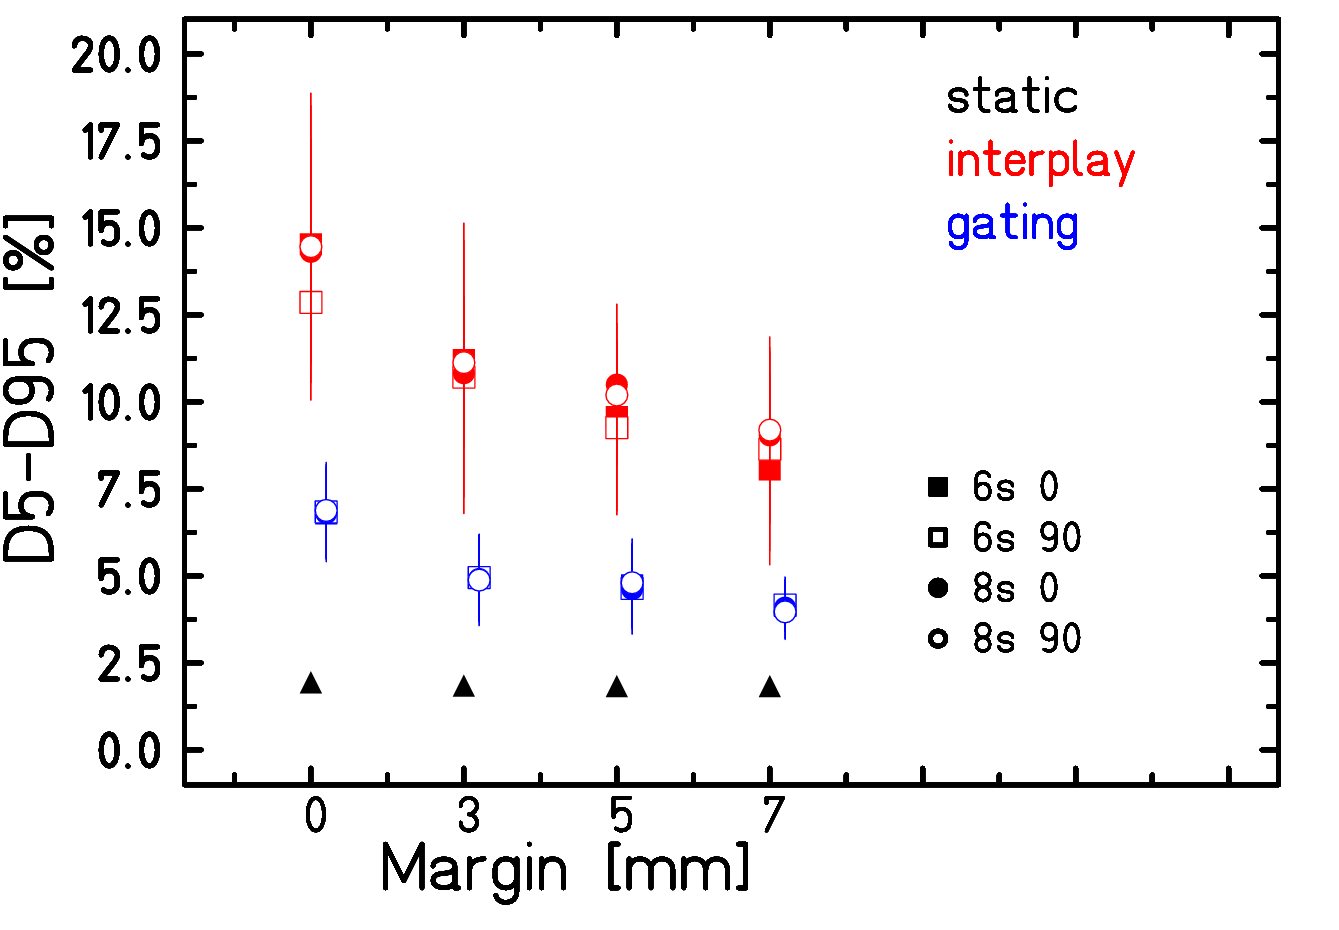
\includegraphics[scale=0.18]{./teile/results_mdacc/MDACC_CTV_LPV_D5D95.png}
 }
 \subfigure[D5-D95: RPV]{
 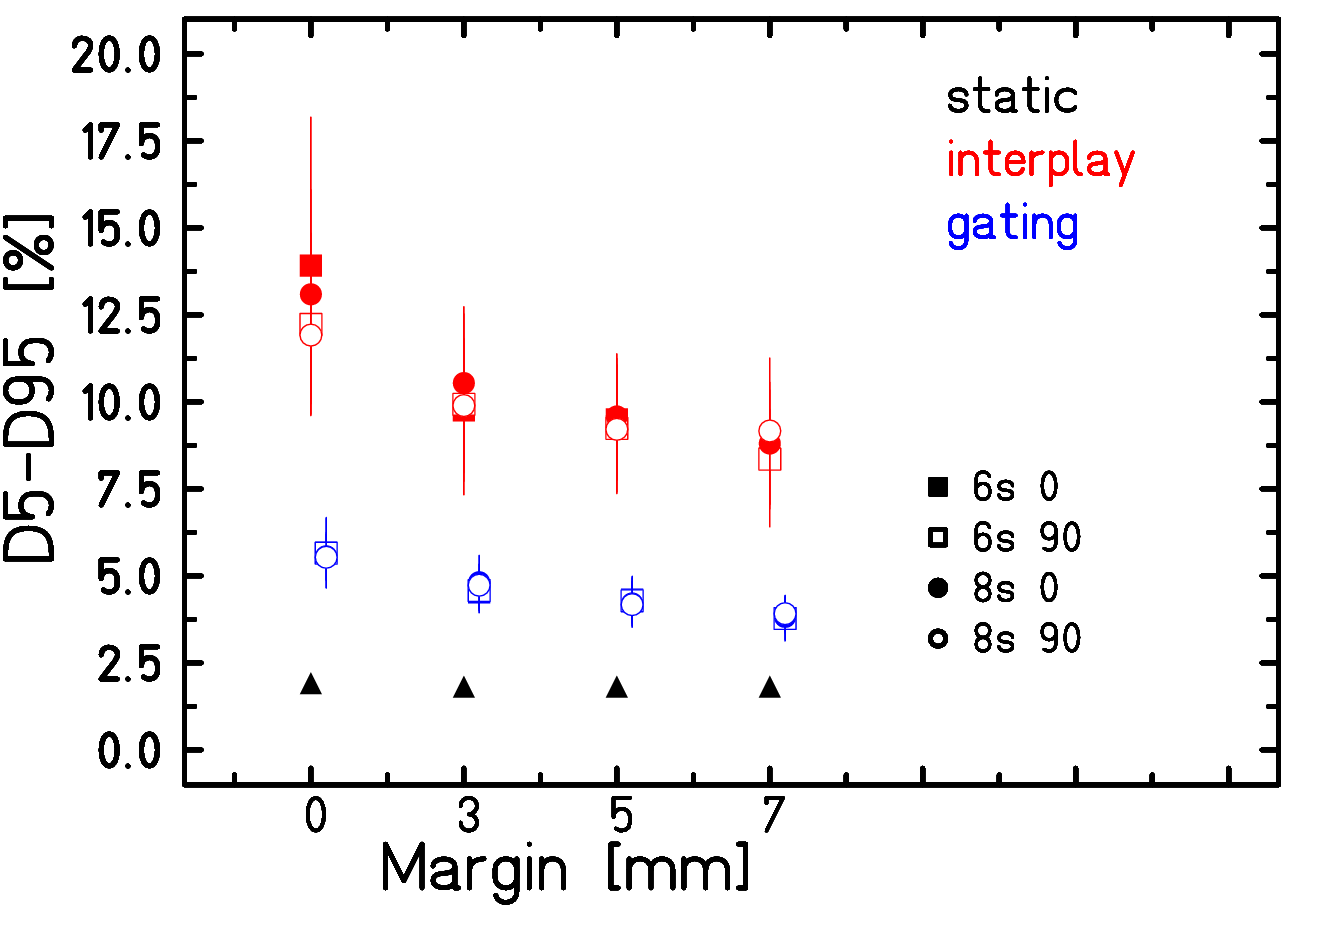
\includegraphics[scale=0.18]{./teile/results_mdacc/MDACC_CTV_RPV_D5D95.png}
 }
 \subfigure[V95: LPV]{
 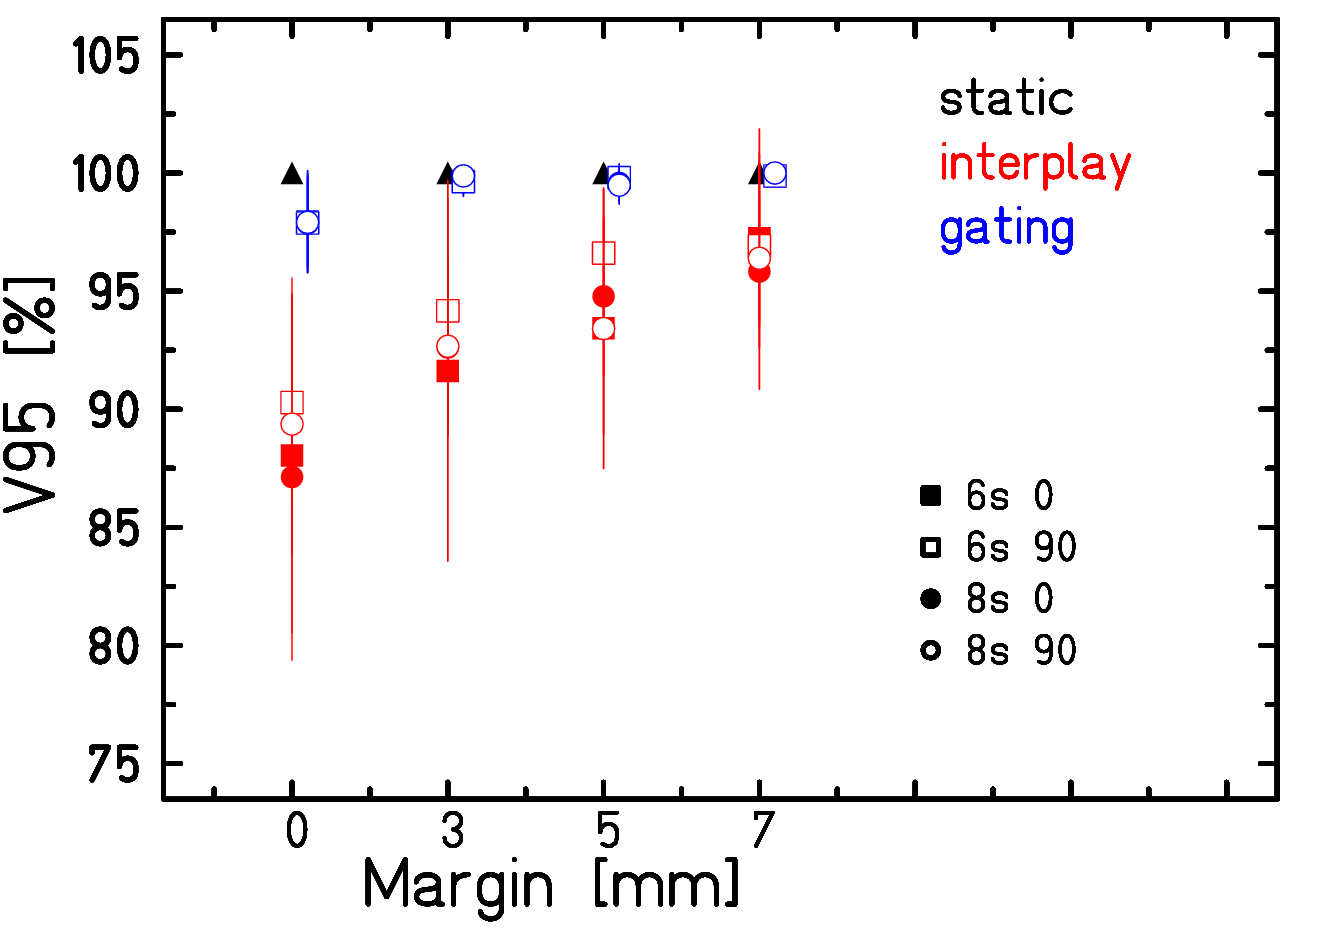
\includegraphics[scale=0.18]{./teile/results_mdacc/MDACC_CTV_LPV_V95.png}
 }
\subfigure[V95: RPV]{
 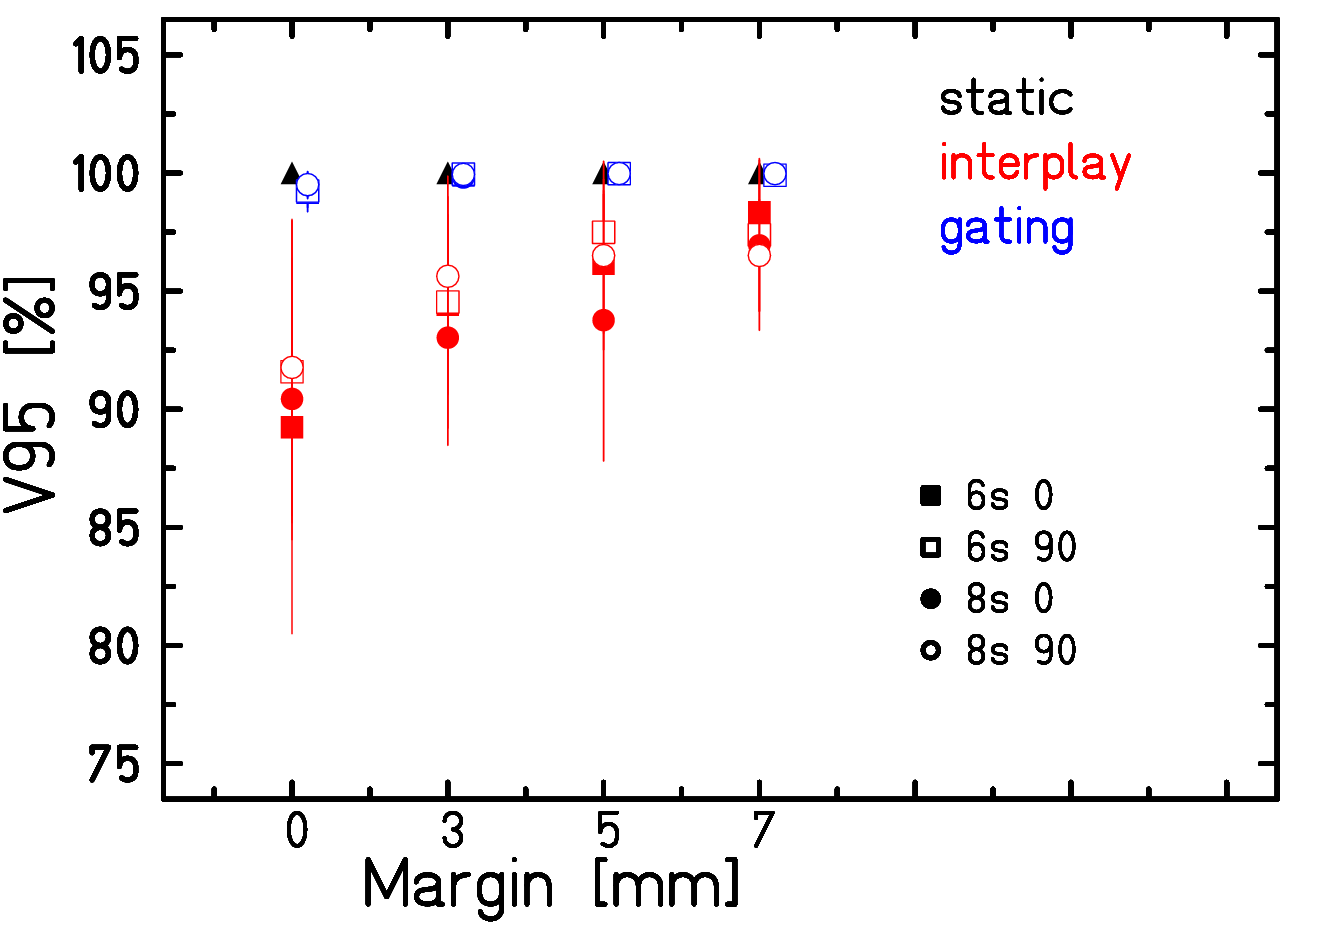
\includegraphics[scale=0.18]{./teile/results_mdacc/MDACC_CTV_RPV_V95.png}
 }
  \subfigure[V107: LPV]{
 \includegraphics[scale=0.18]{./teile/results_mdacc/MDACC_CTV_LPV_V107.png}
 }
\subfigure[V107: RPV]{
 \includegraphics[scale=0.18]{./teile/results_mdacc/MDACC_CTV_RPV_V107.png}
 }
\caption{Mean value and standard deviation of dose analysis parameters D5-D95 (first row), V95 (middle row) 
and V107 (last row) over all patients. The LPV (left column) and RPV (right column) were studied seperately. Static (black) as well as interplay (red) and gating (blue) 
are compared for four different motions and different safety margins.}
\label{static_interplay_gating}
\end{figure}

\newpage 

\begin{figure}[H]
\centering
\subfigure[D5-D95 versus margin size]{
 \includegraphics[scale=0.75]{./teile/results_mdacc/D5D95_vs_margin_2.png}
 }
 \subfigure[V95 versus margin size]{
 \includegraphics[scale=0.75]{./teile/results_mdacc/V95_vs_margin_2.png}
 }
\caption{(a) and (b): Boxplot of dose analysis parameters D5-D95 and V95 over all patient data sets, motion patterns and target volumes (LPV: circle and 
RPV: cross) depending on the used margins size (0mm, 3mm, 5mm and 7mm) and irradiation mode (static, interplay and gating). Here, minimum and 
maximum of the data is plotted within 1.5 times the interquartile range, the other data points are stated as outliers. 
Figures are courtesy of Dr. Christian Graeff.}
\label{static_interplay_gating_ALLpatients_KORR}
\end{figure}

\newpage


\subsubsection*{Rescanning of gated volume}
\label{RescanofGate}

The combination of two motion mitigation techniques, gating and rescanning, would directly apply when not only the respiratory motion but 
also the heartbeat would be compensated for (see chapter \ref{chapter:human}). In order to study the outcome of such a delivery, several 
number of rescans (5, 10, 15 and 20) were applied on the gated irradiation for patient 2 (as an example of a patient with a medium absolute 
displacement of the target volumes) and patient 9 (with the highest studied absolute displacement). The results can be seen in figure 
\ref{static_interplay_gating_rescan_Pat02} and \ref{static_interplay_gating_rescan_Pat09}. For patient 9 the DVHs for static as well as 
the gating results for all motion patterns and the corresponding results for ten rescans within the gating window are shown in 
figure \ref{dvhs_pat09_mdacc_rescan}. All numerical results are shown in appendix \ref{app:mdacc} (tables \ref{tab:pat02:LPV:rescan} to 
\ref{tab:pat09:RPV:rescan}).\newline
\newline
It becomes obvious that rescanning does further improve the dose delivery regarding dose homogeneity. For patient 2 the 
dose homogeneity value of 6.8\% of the prescribed physical dose of 25Gy achieved with gating in the LPV (3 mm margin, motion period of 6s and starting 
phase of 90$^{\circ}$) can be slightly improved to 4.7\% with five rescans or 3.8\% with ten rescans. In RPV the dose homogeneity value of 
patient 2 of 5.0\% for the same margin and motion can be improved to 4.8\% with five rescans and 4.1\% with ten rescans. 
For patient 9 the dose homogeneity value of 5.0\% for LPV with 3mm margin and motion period of 6s, starting phase of 90$^{\circ}$ can 
be improved to 3.8\% with five rescans. For the RPV dose homogeneity of 4.4\% with the same margin and motion can be reduced to 
3.9\% with five rescans. Rescan numbers higher than ten only lead to a minor improvement. For example in Patient 9 the LPV irradiation with 
3mm margin and the stated motion of 6s period and 90$^{\circ}$ starting phase results in 3.7\%, both for fifteen and twenty rescans, 
respectively.\newline
\newline
It can be concluded that the dose homogeneity can be slightly improved with rescanning within the gating window. A small number of rescans, 
e.g. five or ten, are already sufficient to yield acceptable results and the outcome can not be improved by using higher rescan numbers. 
As rescanning will be studied as motion mitigation technique for the heartbeat motion influence, the overlay of rescanning and gating will be 
carried out automatically in case of an application of the here studied non-invasive treatment modality for atrial fibrillation, as both, 
respiration and heartbeat, need to be accounted for. 

\newpage

\begin{figure}[H]
\subfigure[D5-D95: LPV]{
 \includegraphics[scale=0.18]{./teile/results_mdacc/MDACC_Pat122_CTV_LPV_D5D95_withRescan.png}
 }
 \subfigure[D5-D95: RPV]{
 \includegraphics[scale=0.18]{./teile/results_mdacc/MDACC_Pat122_CTV_RPV_D5D95_withRescan.png}
 }
 \subfigure[V95: LPV]{
 \includegraphics[scale=0.18]{./teile/results_mdacc/MDACC_Pat122_CTV_LPV_V95_withRescan.png}
 }
\subfigure[V95: RPV]{
 \includegraphics[scale=0.18]{./teile/results_mdacc/MDACC_Pat122_CTV_RPV_V95_withRescan.png}
 }
  \subfigure[V107: LPV]{
 \includegraphics[scale=0.18]{./teile/results_mdacc/MDACC_Pat122_CTV_LPV_V107_withRescan.png}
 }
\subfigure[V107: RPV]{
 \includegraphics[scale=0.18]{./teile/results_mdacc/MDACC_Pat122_CTV_RPV_V107_withRescan.png}
 }
\caption{Patient 9: Dose analysis parameters for LPV (left column) and RPV (right column). Besides static (black), interplay (red) and gating 
(blue) also different rescan numbers on the gated irradiation were applied (five (green) and ten rescans (orange)). The results are compared for four different 
motions and different safety margins. For a better visualization the rescanning data points for each motion pattern are shifted and the result 
for fifteen and twenty rescans are not displayed.}
\label{static_interplay_gating_rescan_Pat09}
\end{figure}

\newpage

 \begin{figure}[H]
 \begin{center}
\subfigure[LPV]{
 \includegraphics[scale=0.48]{./teile/results_mdacc/Pat09_allDVHs_LPV_rescan_withLegend.png}
 }
\subfigure[RPV]{
 \includegraphics[scale=0.48]{./teile/results_mdacc/Pat09_allDVHs_RPV_rescan_withLegend.png}
 }
\caption{Dose volume histograms for CTV of patient 9 for 3mm safety margin irradiation (LPV (a) as well as RPV (b)) in case of static 
irradiation (black), gating (solid) and five rescans inside the gating window (dashed). The motion patterns are shown in colors (6s 0: lujan motion with period of 6s 
and starting phase 0$^{\circ}$, 6s 90: lujan motion period of 6s and starting phase 90$^{\circ}$, 8s 0: lujan motion period of 8s 
and starting phase 0$^{\circ}$, 8s 90: lujan motion period of 8s and starting phase 90$^{\circ}$.}
\label{dvhs_pat09_mdacc_rescan}
 \end{center}
\end{figure}

\newpage

\begin{figure}[H]
\subfigure[D5-D95: LPV]{
 \includegraphics[scale=0.18]{./teile/results_mdacc/MDACC_Pat024_CTV_LPV_D5D95_withRescan.png}
 }
 \subfigure[D5-D95: RPV]{
 \includegraphics[scale=0.18]{./teile/results_mdacc/MDACC_Pat024_CTV_RPV_D5D95_withRescan.png}
 }
 \subfigure[V95: LPV]{
 \includegraphics[scale=0.18]{./teile/results_mdacc/MDACC_Pat024_CTV_LPV_V95_withRescan.png}
 }
\subfigure[V95: RPV]{
 \includegraphics[scale=0.18]{./teile/results_mdacc/MDACC_Pat024_CTV_RPV_V95_withRescan.png}
 }
  \subfigure[V107: LPV]{
 \includegraphics[scale=0.18]{./teile/results_mdacc/MDACC_Pat024_CTV_LPV_V107_withRescan.png}
 }
\subfigure[V107: RPV]{
 \includegraphics[scale=0.18]{./teile/results_mdacc/MDACC_Pat024_CTV_RPV_V107_withRescan.png}
 }
\caption{Patient 2: Dose analysis parameters for LPV (left column) and RPV (right column). Besides static (black), interplay (red) and gating 
(blue) also different rescan numbers on the gated irradiation were applied (five (green) and ten rescans (orange)). The results are compared 
for four different motions and different safety margins. For a better visualization the rescanning data points for each motion pattern are 
shifted and the result for fifteen and twenty rescans are not displayed.}
\label{static_interplay_gating_rescan_Pat02}
\end{figure}

\newpage


\subsubsection{Irradiation time}

One of the disadvantages of gating as motion mitigation technique is that the irradiation time is increased depending on the used gating window 
size. When a gating window of roughly 30\% is used, like in this study, the irradiation is prolonged by a factor of three compared to the static 
irradiation. In figure \ref{irrTime_gating_Pat024} the needed irradiation time for the gated irradiation of LPV and RPV in patient 2 is shown for 
different safety margins and motion patterns. The duration for each beam entry channel (gantry angle of -45$^{\circ}$, 135$^{\circ}$ and 0$^{\circ}$) 
is plotted individually. On the left side the duration of an irradiation with a small minimal particle number (11,000 particles per beam spot) 
is shown, while on the right side an irradiation with a higher minimal particle number (55,000 particles per beam spot) is displayed. 
Even though a higher intensity is expected to result in a shorter treatment time and would hence be favorable for the efficiency of the 
treatment, it was shown that very high intensities endanger a homogenous dose coverage \cite{Mue14}. The usage of lower intensities is 
hence motivated and needs to be studied in the individual cases.\newline
\newline
As expected, the needed irradiation time increases with the used safety margin as the irradiated volume increases. Furthermore 
the irradiation time is independent of the motion pattern but varies depending on the used beam entry channel. While the low intensity 
irradiation can take up to 120 minutes (for a safety margin of 3mm), the overall duration can be reduced to only 30 minutes (for a safety 
margin of 3mm) for the irradiation with a higher intensity. It should be noted that this is the gating time for the respiratory motion alone 
and the overall treatment time will thus be prolonged, as cardiac motion is not yet compensated for. 

\vspace*{0.6cm}

 \begin{figure}[H]
\subfigure[Patient 2: $N_{\mathrm{min}}$ = 11,000]{
 \includegraphics[scale=0.18]{./teile/results_mdacc/Pat024_all_irrTime.png}
 }
\subfigure[Patient 2: $N_{\mathrm{min}}$ = 55,000]{
 \includegraphics[scale=0.18]{./teile/results_mdacc/Pat024_all_irrTime_hoheNmin.png}
 }
\caption{Irradiation time for gating for patient 2 for different intensities, different 
safety margins, underlying motion patterns and beam entry channels.}
\label{irrTime_gating_Pat024}
\end{figure}



\newpage

\section{Discussion}
In this chapter the influence of respiratory motion on the PVs was studied and treatment planning studies with gating as motion 
mitigation technique were carried out. Respiration was found to be an important motion component for the treatment of cardiac volumes. 
Recent studies in the cardiology community also indicate that real time compensation of breathing displacement 
would even be beneficial for catheter ablation \cite{Kum12, Frie12}.\newline
\newline
Different studies on the influence of respiration on the PV motion exist as they are of interest for image guided ablation procedures. 
Thereby relative displacements (like deformation or splaying of the PVs) and absolute motion (translational and rotation) are distinguished. 
Noseworthy et al. \cite{Nos05} studied the relative changes in the PV anatomy during the breathing cycle. They thereby investigated the changing 
branching angle between the inferior and superior LPV (LIPV, LSPV) and RPV (RIPV, RSPV), respectively. They stated that the PV splay increased 
during inspiration (branching angle of RPVs increased from (40 $\pm$ 10)$^\circ$ to (60 $\pm$ 15)$^\circ$ and for LPVs 
from (50 $\pm$ 11)$^\circ$ to (62 $\pm$ 13)$^\circ$). Furthermore they found a significant reduction in 
the diameter of the RIPV and RSPV during inspiration. Ector et al. \cite{Ect08} on the other hand stated that they only found a slight, 
but significant diameter reduction in the RIPV. In their paper they furthermore studied the absolute translational motion. 
Their patient cohort had a mean diaphragmatic movement of (35 $\pm$ 16)mm for the right diaphragm, resulting in an absolute mean displacement 
for both LPV and RPV of (19.1 $\pm$ 8.6)mm. The mean inferior motion was stated 
to (14.6 $\pm$ 7.7)mm, in anterior direction to (9.7 $\pm$ 7.6)mm and the smallest motion direction was the leftward direction with 
(0.4 $\pm$ 3.8)mm. Comparing motion patterns between veins the LPVs were found to move less in anterior direction then the RPVs, but did 
not differ significantly in other directions. They found a strong association between diaphragmatic motion and inferior PV motion.\newline
\newline
In the here studied patient cohort of lung cancer patients a much smaller mean absolute displacement of the pulmonary veins was found over all 
patients with (6.8 $\pm$ 3.6)mm for LPV and (6.8 $\pm$ 2.5) for RPV. The SI motion had a mean value of (-6.4 $\pm$ 3.8)mm and 
(-6.6 $\pm$ 2.4)mm for RPV, respectively. In AP direction the mean amplitude for all patients was (-0.8 $\pm$ 0.5)mm for LPV and 
(-0.9 $\pm$ 0.8) for RPV, which corresponds to the finding by Ector et al. that the LPV move less in anterior direction than the RPV. For LR 
direction a mean displacement of (-0.9 $\pm$ 0.9) of LPV and (0.5 $\pm$ 1.0)mm of RPV was found over all patients. 
Contrary to Ector et al. a significant difference in the motion of the LPV compared to RPV was hence found in LR. 
A correlation between diaphragm motion and PV displacement was only found in the RPV (r=0.79, p<0.05). Even though a similar result was 
expected for the LPV, no correlation was observed here. It is unclear if this is due to location of the ablation site or due to the 
underlying lung cancer patient data in comparison to AF patient data sets.\newline
\newline
Recent studies in the cardiology community \cite{Kum12} concluded that also for catheter ablation respiration plays an important role as it may 
reduce the catheter tip contact force. Consideration of respiratory motion is thus recommended. Besides ventilation and apnea, Friedmann 
\cite{Frie12} also states that jet ventilation or breath-hold might be adequate strategies for catheter ablation. Even though these techniques 
may also be options for a non-invasive treatment of atrial fibrillation with a scanned carbon ion beam, gating was 
studied as a motion mitigation technique in the present work. In irradiation of cardiac volumes in the animal studies carried out 
at CyberHeart and at the Universit\"atsklinikum Schleswig-Holstein in L\"ubeck different approaches were used. While Blanck et al. 
\cite{Bla13} used an ITV approach for the respiratory motion, Sharma et al. \cite{Sha10} tracked the respiration with the underlying 
CyberKnife Synchrony software (see chapter \ref{chapter:intro}, section \ref{Motionacq}). For particle therapy tracking is not feasible yet as 
no fast and precise real-time internal motion monitoring including particle range information exists. A simple enlargement of internal margins 
to produce an ITV for respiration was withdrawn due to expected high dose deposition in critical OAR close to the target sites 
(see chapter \ref{chapter:human}). Gating offers the advantage of a currently technical feasibility while keeping the dose to the normal 
tissue relatively small. Nevertheless it leads to a prolongation of the treatment time. However, with a high intensity of 55,000 minimum 
particles per spill a duration of only 30 minutes could be achieved (patient 2, safety margin of 3mm). This already offers a reduced 
treatment time compared to the results by Sharma et al. where a treatment time of one to two hours was estimated. 
While lower intensities lead to a longer treatment time, it is nevertheless known from previous studies \cite{Mue14} that high intensities 
can result in inhomogeneous dose depositions. Other methods to reduce the treatment time might hence be needed in order to still guarantee a time 
efficient delivery. Tsunashima et al. \cite{Tsu08} studied cyclotron settings that could lead to a reduced treatment time in particle gating. 
They thereby found that variable excitation cycles, in synchrony with the respiratory pattern of the patient, could reduce the treatment time 
prolongation to a factor two, instead of the usual factor three, for a 30\% gating window. 
Iwata et al. \cite{Iwa10b} furthermore proposed a method to reduce the needed time for energy changes inbetween IESs in synchrotrons. 
By using radiofrequency knockout exciters and multiple energy operation patterns, the beam would be accelerated to the maximum energy and than 
stepwise decelerated to lower energies, using an extension of the respective flattops to extract the particles with varying energies during a 
single operation cycle of the synchrotron.\newline
\newline
Concerning the dose deposition with gating compared to interplay it can be concluded that gating yields good dose coverage. The V95 values 
were higher than 99\% for all target sites with safety margin of 3mm or more and higher than 95\% in all cases without safety margin (minimum of 
95.21\% in patient 9 for LPV, no safety margin and motion period of 8s, starting phase of 0$^{\circ}$).The V107 values were all smaller 
than 0.1\% (maximum of 0.1\% for patient 2, RPV, in case of 5mm margin and motion with period of 8s and starting phase of 90$^{\circ}$). 
Hence an acceptable dose coverage could be achieved. The dose homogeneity did not exceed 9.18\% without safety margin (patient 5, LPV, no 
safety margin and motion period of 8s, starting phase of 90$^{\circ}$). With safety margin, the D5-D95 value did not exceed 8\%. An additional 
safety margin is thus beneficial to guarantee a robust and successful treatment delivery. However, an extension of the target volume due to 
safety margins always results in more dose to the normal tissue and to potential critical OARs. A limited safety margin of 3mm or 5mm would 
offer the benefit of improved treatment outcome while keeping the irradiated volume low (see also chapter \ref{chapter:human}).\newline
\newline
Rescanning within the gating window could slightly improve the results for dose homogeneity as it reduces the influence of residual motion 
inside the gating window. The dose homogeneity in the LPV of patient 9 for example (large motion amplitude) could be reduced from 5.01\%  
(safety margin of 3mm, motion period 6s and 90$^{\circ}$ starting phase) to 3.83\% with five rescans. 


\section{Conclusion}

The PVs were found to move due to respiration with an amplitude of up to 2cm. 
This displacement creates interplay effects when irradiated with scanned carbon ions. Gating as motion mitigation technique was studied. 
It can be concluded that this method yields improved dose coverage (under and over dosage) and better dose homogeneity compared to interplay 
in all studied patient cases, for all motion patterns and safety margins and achieves results comparable to the static irradiations. 
It can thus be an adequate motion mitigation technique for the irradiation of PVs under influence of respiratory motion. 
As rescanning is a potential technique when compensating for displacements due to 
heartbeat (see chapter \ref{chapter:human}), the combination of these two motion mitigation technique could be feasible in a potential 
application. Hence rescanning inside the gating window was studied and it was shown that a  small number of rescans (e.g. five or ten) are 
sufficient to improve the results of dose homogeneity. 



%%%%%%%%%%%%%%%%%%%%%%%%%%%%%%%%%%%%%%%%%%%
%%%%%%%%%%%%%% APPENDIX %%%%%%%%%%%%%%%%%%%
%%%%%%%%%%%%%%%%%%%%%%%%%%%%%%%%%%%%%%%%%%%



  
  \setcounter{mtc}{3}
  
% \chapter{Treatment planning study for irradiation of pulmonary veins under influence of heartbeat motion in human data}
\chapter{Irradiation of pulmonary veins under influence of heartbeat in human data}
\label{chapter:human}
\minitoc

The PVs move on one hand due to the heartbeat and on the other hand due to respiration of the patient. 
Both motion types are independent from each other and can hence be studied individually. While the influence of respiration is analyzed in 
chapter \ref{chapter:mdacc}, the effect of heartbeat motion will be discussed in this chapter. 
CTs of five AF patients, gated to the complete cardiac cycle in end-expiration, were acquired at Mayo Clinic (Rochester, Minnesota, USA). 
The motion direction as well as motion amplitude of LPV and RPV were studied for all cases. 
Motion influences on accuracy and homogeneity of the dose delivery in the PVs were studied using these data. 
The resulting interplay pattern for all patients as well as 
rescanning as possible motion mitigation technique have been analyzed and the results will be presented in this chapter. 

\section{Material and methods}
The input data as well as the treatment planning parameters will be stated before all conducted studies will be specified. 
The analysis procedure will be explained.  


\subsection{Treatment planning input data}
As was already stated in chapter \ref{chapter:mdacc} 4DCT data sets, segmentation of the target volumes and OARs and deformable image 
registrations in-between the different motion phases are needed for the here presented treatment planning studies using the in-house software 
TRiP4D \cite{Ric13}.\newline
\newline
In order to study the displacement of the PV due to heartbeat ECG gated 4DCTs in end exhale (breath hold) were studied. 
Five AF patient data sets (four male patients and one female) were recorded and anonymized at Mayo Clinic (Rochester, Minnesota, USA). 
The CT scans were acquired on a Sensation 64 CT scanner (Siemens). Each of the 4DCT data set consisted of twenty temporal equally distributed 
cardiac motion phases, the reference phase zero started at the R-peak of the QRS-complex (see chapter \ref{chapter:intro}, section \ref{HCS}). 
In order to distinguish structures within the heart the CT scans were contrast enhanced. The radiopaque material was administered intravenously (150cc Omnipaque 350 at 4cc/sec). 
Segmentation of the target volumes (LPVs and RPVs) as well as the OAR (esophagus, trachea, aorta and cardiac structures) were carried out by a 
collaborating cardiologist at Mayo Clinic on the reference 4DCT phase with Eclipse\texttrademark (Varian Medical Systems). The volumes of the 
contours for the ablation sites for LPV and RPV are presented for each patient in table \ref{tab:volume:mayo}. 

\begin{table}[htbp]
  \centering
  \caption{Target volume for LPVs and RPVs for all investigated patients.}
  \begin{tabular}{|c|c|c|}
    \hline\hline
    patient no\rule{0pt}{2.6ex}\rule[-1.2ex]{0pt}{0pt} & LPV [cm$^{3}$] & RPV [cm$^{3}$]\\
    \hline
    1 & 2.03 & 2.39 \\
    2 & 2.62 & 5.16 \\
    3 & 1.45 & 4.16 \\
    4 & 1.66 & 2.07 \\
    5 & 2.06 & 1.90 \\
    \hline\hline
  \end{tabular}
  \label{tab:volume:mayo}
\end{table}

Non-rigid image registration of the nineteen motion phase on the reference phase have been performed with Plastimatch \cite{Sharp07, Shack10}. 
Here the first step of the B-spline registration was carried out with 50 maximal iterations and an isotropic 
spacing of 20mm was chosen. The second step was carried out with 100 maximal iterations and the grid spacing was set to 3mm. 
The regularization was chosen to be $\lambda$=0.0001. The same visualization techniques as stated in chapter \ref{chapter:mdacc} were used for 
a quality assurance of the registration (false color images \cite{Bro07}, checker board images \cite{Bro07} and a qualitative check of the 
vector field regularization). The stated tests were carried out on the one hand between motion phase 3 (the motion phase of the 
maximal ventricular displacement) and the reference phase (motion phase zero) and on the other hand between motion 
phase 18 (maximal displacement of the atria) and the reference phase.  

\vspace*{-0.5cm}

\subsection{Treatment planning parameters}
\label{human:tpp}
Also here 3D (static) and 4D treatment plans were generated. For informations on the dose optimization process, the ITV generation 
with the implementation of the studied safety margins (3mm, 5mm and 7mm), the used raster spacing and the dose 
algorithm the reader should be referred to \ref{mdacc:tpp}.\newline
\newline
All treatment plans were calculated as intensity modulated particle therapy (IMPT). Part of the study included the 
esophagus as critical structure in the optimization process (IMPT(OAR)). Thereby two different dose restrictions to this OAR were used. 
In one part of the calculations it was stated that the esophagus should not receive more than 70\% of the physical dose. 
The strength of this restriction was determined by a weightfactor, which was set to 75\%. In a second iteration the restrictions were stronger and 
the maximal physical dose to this structure was set to 30\% with a weighting factor of 200\%. 
Also here a physical dose of 25Gy was applied in one fraction in all simulations. Since potential biological 
effects were not included in the studies the applied dose is linear and the results, e.g. dose depositions to critical structures, can be 
scaled to other dose values \footnote{only limited by the minimal particle fluence per beam spot}.\newline
\newline
The generation of treatment plans is furthermore also dependent on the theoretically possible 
beam application. Spill length, shape and particle intensity are thus important factors. For the here presented simulations GSI accelerator 
parameters have been used. Thereby a spill length of 2.2s is assumed. The pause in between spills is either 2.2s, when no energy change is 
required afterwards, or 3.2s when an energy change is needed. The spill shape is approximated by a Gaussian function. The particle intensities 
feasible at GSI vary between 2x10$^{6}$ and 2x10$^{8}$ particles per spill. Inbetween these two extreme intensity levels, 
fifteen different intensity levels can be used. In the resulting treatment plan, the intensity steps are automatically chosen \cite{Krae00, Ric13}. 
The minimum particle number per beam spot was set to 5,000.\newline
\newline
As the reconstruction of the 4DCTs was based on the time scale a phase-based motion state detection was employed. 
In order to consider possible divergence in the heartbeat motion pattern of patients, different periods (1s and 0.7s) as well as 
different starting phases (0$^{\circ}$ and 90$^{\circ}$) were used. The motion periods were chosen according to the heartbeat rate of 
60 to 80 beats per minute. 


% \newpage

\subsubsection{Field number and beam directions}

The field number and directions were systematically investigated and are listed in table \ref{tab:fields}. 
Four different field numbers 
(one to four) were studied. While for one field the gantry angle was kept constant to 0$^{\circ}$ and only the couch angle was 
changed, for higher field numbers different gantry angles were used. These angles are illustrated in figure \ref{gantrydirection}. 


\begin{table}[H]
  \centering
     \small
  \caption{Studied field number and beam channel directions}
  \begin{tabular}{|c|c|c|}
    \hline\hline
    Field number & Couch angle [$^{\circ}$] & Gantry angle [$^{\circ}$]\\
    \hline 
1 field & -90 & 0 \\
& -45 & 0 \\
& -135 & 0 \\
\hline
2 fields & 90 & -60/120 \\
& 90 & -60/135 \\
& 90 & -60/0 \\
& 90 & -45/135 \\
& 90 & -45/150 \\
& 90 & -45/0 \\
\hline
3 fields & 90 & -60/120/150 \\
& 90 & -60/120/0 \\
& 90 & -45/135/150 \\
& 90 & -45/135/0 \\
\hline
4 fields & 90 & -60/120/-45/135 \\
& 90 & -60/120/0/180 \\
& 90 & -45/135/0/180 \\
& 90 & -160/90/-60/145 \\
    \hline\hline
  \end{tabular}
  \label{tab:fields}
\end{table}

\vspace*{-0.6cm}

\begin{figure}[H]
 \begin{center}
  \includegraphics[scale=0.4]{./teile/results_human/GantryDirection_BEV.png}
  \caption{Entry channels for different gantry directions for a couch angle of 90$^{\circ}$. The beam's eye view (BEV) is marked.}
  \label{gantrydirection}
 \end{center}
\end{figure}


\newpage


\subsection{Treatment planning studies}

Besides representing a reference value for the 4D cases, 3D treatment plans were also generated here 
in order to find the best suited combinations of beam entry channels as well as to study possible safety margin limitations. In order to find 
a suitable field number and beam direction for the 4D treatment planning 
studies, static simulations on the original CTV volume (LPV together with RPV) with the above mentioned treatment planning parameters were 
carried out for all five patients. 17 different beam channel combinations were studied (see table \ref{tab:fields}). As a criteria for the 
best possible solution the dose to OAR was assessed. Furthermore, different ITV margins (original and increased with 3mm, 5mm and 7mm margin) 
were studied in 3D treatment plans for all patients. The resulting dose depositions were compared to dose deliveries with the same margins 
where the esophagus was included in the optimization process. Possible limitations were again analyzed according to the dose deposition in the OARs. \newline
\newline
In order to prepare for the 4D simulations, the motion of the PVs due to heartbeat was assessed. 
4D plans were distinguished between an underlying motion without any compensation, resulting in interplay patterns \cite{Phi92, Ber08}, 
and with the application of rescanning \cite{Phi92} as motion mitigation technique. For rescanning different rescan numbers 
(5, 10, 15 and 20) were compared. Static, interplay as well as rescanning treatment plans for all patients were carried out with one 
beam channel combination (couch angle of 90$^{\circ}$ and gantry angles of -45$^{\circ}$, 135$^{\circ}$ and 0$^{\circ}$), all four safety 
margins, the stated treatment planning parameters and the four stated motion trajectories. 


\subsection{Analysis}

Both the dose deposition in OAR as well as dose homogeneity in the target volume were studied. For the OAR dose-volume restrictions in 
esophagus, trachea, aorta and the whole heart were compared to values from RTOG study protocols (see next paragraph). 
As further OARs cardiac substructures (ventricles and coronary arteries) were studied. 
For comparison of the resulting dose coverage in the target region dose-volume-histograms (DVHs) were studied. Furthermore 
motion-volume-histograms (MVHs) \cite{Ric13} were generated displaying the relative displacement of every voxel of the investigated volume to 
the reference phase in all three motion directions. With these values the resulting motion of the PVs due to heartbeat could be assessed. 

\newpage

\subsubsection{Dose-volume constraints for organs at risk}
\label{human:dose-volumeOar}
The dose deposition in the OAR is an important limitation and selection criteria when studying the field number and beam channel 
direction as well as the possible safety margin limitations. Since a single fraction of 25Gy or higher is assumed to be used in this 
non-invasive treatment modality, dose tolerance limits used in stereotactic body radiotherapy (SBRT) are highly related \cite{Ber12}. An 
extensive collection of dose-volume-limits for SBRT are presented in Grimm et al. \cite{Gri11} and the AAPM Task Group Report \cite{AAPM10}.  
Both are literature reviews of limits utilized and reported in existing publications. For the OAR in the here presented 
treatment planning study (esophagus, trachea, heart and aorta) the dose-volume-limits in both literature reviews were taken from the 
Radiation Therapy Oncology Group (RTOG). The RTOG is a national clinical cooperative group of over 360 institutions across the United 
States and Canada, which was funded by the National Cancer Institute (NCI) \cite{RTOG}. In their study protocols RTOG 0631 
(a phase II/III trial of SBRT for localized spine metastasis) \cite{RTOG0631} and RTOG 0915 (a randomized phase II trial of SBRT for 
medically inoperable patients with stage I peripheral non-small cell lunger cancer) \cite{RTOG0915} the following dose-volume-limits 
were stated (see table \ref{tab:RTOG}). 

\vspace*{-1cm}

\begin{table}[H]
  \centering
  \footnotesize
  \caption{Dose-volume limits for OAR.}
  \begin{tabular}{|c|c|c|c|}
    \hline\hline
    OAR & Volume [cc] & Dose [Gy] & endpoint \\
    \hline
    Aorta / great vessels & 10 & 31 & Aneurysm \\
    Esophagus & 5 & 11.9 &  Stenosis / fistula \\
    Heart & 15 & 16 & Pericarditis \\
    Trachea & 4 & 10.5 & Stenosis / fistula \\
    \hline\hline
  \end{tabular}
  \label{tab:RTOG}
\end{table}

\vspace*{-0.3cm}

Since the heart is not only a critical organ but also the target site in this treatment modality, further differentiation of 
limits depending on the substructures of the heart are needed. Unfortunately, data on this topic is scarce. Literature on cardiac disease 
resulting from radiation exposure mostly relies on cancer patient data treated with radiotherapy (in particular breast cancer and Hodgkin's 
lymphoma) or atomic bomb survivors. Besides the stated dose-volume limitation, the mean dose and maximum point dose to the whole heart was 
studied. Furthermore the maximal irradiated heart volume (V$_{>0}$) was examined. 
Concerning substructures the left and right ventricle as well as the coronary arteries were analyzed for mean and maximum dose deposition and 
maximal irradiated volume contribution. Since the values were not normally distributed, boxplots were generated, where the median (50th 
percentile), the 25th and 75th percentile and the minimum and maximum values over all patient cases are displayed. 

\subsubsection{Dose deposition in target volume and motion of PVs}

The V95, V107 as well as D5-D95 of the CTVs were analyzed. 
The stated values have been evaluated for all beam applications (static, interplay, rescanning). 
Futhermore the median and percentile values of these parameters over all studied motion patterns and patient cases were 
generated. The relation of dose analysis parameters to different margin sizes and rescanning number was analyzed by a one-way ANOVA and 
the proportion of variance explained $r^{2}$ is reported with the corresponding p-value ($p$<0.0001). 


\vspace*{-0.3cm}

\section{Results}

In the following the results of the beam direction and safety margin study, of PV motion assessment as well as of the treatment planning studies 
will be discussed. As a criteria for an adequate field number and beam channel direction as well as safety margin limitation the dose to OAR 
will be presented. The motion due to heartbeat is shown. For the treatment planning study different dose analysis parameters will be presented 
and compared for different cases (static, interplay and rescanning). 

\vspace*{-0.3cm}

\subsection{Beam direction}
\label{human:beamdirection}
In figures \ref{beamdirection_boxplot} and \ref{beamdirection} the resulting dose to the pertinent OARs is shown for all studied beam 
directions and patients. Figure \ref{beamdirection_boxplot} displays the results as a boxplot over all patient cases for a respective field 
number (and hence different beam directions) while figure \ref{beamdirection} shows the individual results for each patient and beam direction. 
The corresponding volumes result from the dose volume limits (see table \ref{tab:RTOG}, represented by a dashed line in the plots). 
In all studied cases, the difference between different beam directions for a certain patient is rather small, resulting in no obvious 
preferable beam direction for the five studied patients. For the four studied OAR it becomes furthermore obvious that while trachea and aorta 
are well spared for almost all beam directions in all patients, esophagus and in particular the heart are much more 
critical.\newline
\newline
In the esophagus the median dose over all patients is 7.8Gy (75th percentile: 9.0Gy) for one field, 11.0Gy (14.1Gy) for 
two fields, 11.0Gy (13.9Gy) for three and 8.0Gy (11.9Gy) for four fields. The result is dependent on the underlying patient anatomy. 
While the majority of the beam directions for patient 1, 4 and 5 remain under the respective dose-volume limit, many plans for patient 2 and 3 
exceed the dose-volume constraints. For these patients dose depositions of 11.9Gy or less are achieved in only about 98\% and 65\% of 
studied cases (patient 2 and 3, respectively). While a single field yields acceptable dose deposition in the esophagus, the beam channel 
results in higher dose depositions in the heart and cardiac substructures like the coronary arteries (see 
figure \ref{beamdirection_MeanMaxD_MaxV} and \ref{beamdirection_MeanMaxD_MaxV_boxplot}) and are thus 
inapplicable. For patient 2 higher field numbers and thus more beam directions result in dose limit exceeding depositions. Due to this 
result the esophagus was included in the optimization of the treatment delivery (IMPT(OAR)). This was studied in comparison 
to a simple IMPT irradiation (see section \ref{safetymarginlimitation}).

%%%%%%%%%%%%%%%%%%%%%%%%%
%%%%%%%% DOSE TO OAR
%%%%%%%%%%%%%%%%%%%%%%%%%

\newpage

\vspace*{2cm}

\begin{figure}[H]
\subfigure[Esophagus]{
 \includegraphics[scale=0.18]{./teile/results_human/Whisker_ESO.png}
 }
 \subfigure[Trachea]{
 \includegraphics[scale=0.18]{./teile/results_human/Whisker_TRACHEA.png}
 }
  \subfigure[Heart]{
 \includegraphics[scale=0.18]{./teile/results_human/Whisker_HEARTwoOverlap.png}
 }
  \subfigure[Aorta]{
 \includegraphics[scale=0.18]{./teile/results_human/Whisker_AORTA.png}
 }
\caption{Boxplots of dose-volume data for different field numbers (one to four fields) over all patients and over the 
respective beam directions. The data is plotted for different OARs when irradiating the LPV and RPV as IMPT in the five patient data sets. 
The dose-volume-limit for each critical organ is indicated with a dashed line in each plot, respectively.}
\label{beamdirection_boxplot}
\end{figure}

\newpage

% \vspace*{0.5cm}

\begin{figure}[H]
\subfigure[Esophagus]{
 \includegraphics[scale=0.18]{./teile/results_human/Mayo_Human_BeamDirection_ESO.png}
 }
 \subfigure[Trachea]{
 \includegraphics[scale=0.18]{./teile/results_human/Mayo_Human_BeamDirection_TRACHEA.png}
 }
  \subfigure[Heart]{
 \includegraphics[scale=0.18]{./teile/results_human/Mayo_Human_BeamDirection_HEARTwoOverlap.png}
 }
  \subfigure[Aorta]{
 \includegraphics[scale=0.18]{./teile/results_human/Mayo_Human_BeamDirection_AORTA.png}
 }
\caption{Dose-volume data of different OAR when irradiating the LPV and RPV as IMPT in the five patient data sets (patient 1: black, 2: 
red, 3: blue, 4: green, 5: orange) with different field numbers (1 field, 2 fields, 3 fields, 4 fields) and different beam directions. 
The dose-volume-limit for each critical organ is indicated with a dashed line in each plot.}
\label{beamdirection}
\end{figure}

\newpage

The dose volume limit for the heart is exceeded in all patients for all beam directions (see figure \ref{beamdirection_boxplot} and \ref{beamdirection}). 
As the heart is not only an OAR in this treatment modality, but some of its substructures are also the target itself, a closer analysis of 
the dose deposition in the heart is required. In the first row of figure \ref{beamdirection_MeanMaxD_MaxV_boxplot} and figure \ref{beamdirection_MeanMaxD_MaxV} 
the mean and maximal dose deposition in the whole heart as well as the maximal irradiated volume are shown. The mean dose over all 
patients and beam directions is found to have a median of 1.3Gy (75th percentile: 1.5Gy). The median over the maximum point dose is 26.6Gy (27.1Gy).
Concerning the maximal irradiated volume it can be seen that except for one result less than 30\% of the heart is irradiated in all other cases. 
In the case of couch position 90$^{\circ}$ and gantry angles of -160$^{\circ}$, -90$^{\circ}$, -60$^{\circ}$ and 145$^{\circ}$ these maximal 
volume is drastically increased, and reaches up to 49.9\% for patient 2. Hence this beam channel case (beam channel case 17) will be 
stated separately in the following analysis. The median of the maximal irradiated volume over all patients is 16.8\% (20.5\%), 
excluding beam channel case 17, and 17.4\% (20.8\%) including this case.\newline
\newline
The results for the dose deposition in the cardiac substructures are presented in row two to five of figure \ref{beamdirection_MeanMaxD_MaxV_boxplot} and 
figure \ref{beamdirection_MeanMaxD_MaxV}. For the ventricles (LV: second row, RV: third row), the mean dose to both LV and RV is negligible. 
The maximal point dose on the other hand varies depending on beam direction and patient. Single beam directions yield a high maximal dose 
deposition in the LV as in the case of a couch angle of -90$^{\circ}$ or -135$^{\circ}$ the beam traverses the LV. 
Consequently for these beam directions the maximal dose to the RV is smaller. The overall maximal dose deposition has a median of 
1.4Gy (75th percentile: 7.4Gy) for LV and 1.3Gy (5.0Gy) for RV. Besides some single beam directions no maximal point dose exceeds 11.2Gy and 10.1Gy 
for LV and RV, respectively. Concerning the maximal irradiated volume of the ventricles, it can be stated that the results differ depending on 
the studied patient. In case of the LV patient 2 has a higher irradiated volume compared to the other patients, while for this patient on the 
contrary the RV is better spared than in other patients. Over all patients the LV is irradiated to a higher extend than the RV. For LV the maximal 
irradiated volume over all beam directions and patients has a median of 1.2\% (6.0\%), when excluding the case of beam channel 17 and to 
1.9\% (6.4\%) when including this case. For RV it is 0.2\% (7.6\%) excluding the beam channel case 17 and to 0.2\% (8.3\%) including it.
For the coronary arteries the beam channel 17 also results in the highest irradiated volume. 
Even though the coronary arteries are found on the surface of the whole heart and hence also on the ventricles, the irradiated volume of 
these structures differ from the result of the ventricles. Here the RCA are irradiated to a higher extent than the LCA. 
The median maximal value for the LCA is 15.7\% (28.0\%) including the stated beam channel case 17 and 15.2\% 
(27.4\%) excluding it. For the RCA the median over the maximal value is much higher and found to be 27.9\% (42.4\%) including the beam channel 
case 17 and to 24.8\% (42.1\%) excluding it. For the mean dose deposited in the LCA one and four beam directions result in an increased dose 
deposition, while three fields yield in general a low mean dose for all studied beam directions and patients. The same is true for the maximum 
point dose in the LCA. In the case of RCA, the results seem to be independent of field number and beam direction. Overall the median over the 
mean dose is 0.4Gy (1.0Gy) for LCA and 0.6Gy (1.6Gy) for RCA. For the maximal point dose the median dose deposition over all beam directions 
and patients is 6.8Gy (10.9Gy) for LCA. For the RCA it was found to be 5.4Gy (7.9Gy). \newline
\newline
While it was not expected to find one beam direction feasible for all five patients, it is striking that no beam position results in a clear 
benefit for the OAR of the individual patients. This is due to the challenging position of the PV target site, which is in direct proximity 
to the esophagus and due to the fact that the heart is not only an OAR in this treatment modality, but also the target site itself. 
Nevertheless for the analyzed cardiac substructure, especially the radiosensitive LCA, it can be concluded that three beam channels seem to be 
beneficial for all patients. Regarding the mean dose deposition in the LCA as well as the maximal irradiated heart volume, combined with the 
requirement of a robust treatment and hence the benefit of large gantry angles in between different beam channels, a couch angle of 
90$^{\circ}$ was chosen together with gantry angles of -45$^{\circ}$, 135$^{\circ}$ and 0$^{\circ}$. These beam channel directions were used 
for a closer analysis of safety margin limitation as well as for the treatment planning studies for all patients. 

\newpage

%%%%%%%%%%%%%%%%%%%%%%%%%
%%%%%%%% DOSE TO THE HEART
%%%%%%%%%%%%%%%%%%%%%%%%%

\begin{figure}[H]

\begin{minipage}{0.31\textwidth}
    \begin{overpic}
    [width=\textwidth]{./teile/results_human/Whisker_HEARTwoOverlap_MeanDose.png}
    \put(40,80){Heart}
    \end{overpic} 
\end{minipage}
\hfill
\begin{minipage}{0.31\textwidth}
  \includegraphics[width=\textwidth]{./teile/results_human/Whisker_HEARTwoOverlap_MaxDose.png}
\end{minipage}
\hfill
\begin{minipage}{0.31\textwidth}
  \includegraphics[width=\textwidth]{./teile/results_human/Whisker_HEARTwoOverlap_MaxVolume.png}
\end{minipage}

\hfill

\begin{minipage}{0.31\textwidth}
    \begin{overpic}
    [width=\textwidth]{./teile/results_human/Whisker_LV_MeanDose.png}
    \put(40,80){LV}
    \end{overpic} 
\end{minipage}
\hfill
\begin{minipage}{0.31\textwidth}
  \includegraphics[width=\textwidth]{./teile/results_human/Whisker_LV_MaxDose.png}
\end{minipage}
\hfill
\begin{minipage}{0.31\textwidth}
  \includegraphics[width=\textwidth]{./teile/results_human/Whisker_LV_MaxVolume.png}
\end{minipage}

\hfill

\begin{minipage}{0.31\textwidth}
    \begin{overpic}
    [width=\textwidth]{./teile/results_human/Whisker_RV_MeanDose.png}
    \put(40,80){RV}
    \end{overpic} 
\end{minipage}
\hfill
\begin{minipage}{0.31\textwidth}
  \includegraphics[width=\textwidth]{./teile/results_human/Whisker_RV_MaxDose.png}
\end{minipage}
\hfill
\begin{minipage}{0.31\textwidth}
  \includegraphics[width=\textwidth]{./teile/results_human/Whisker_RV_MaxVolume.png}
\end{minipage}

\hfill

\begin{minipage}{0.31\textwidth}
    \begin{overpic}
    [width=\textwidth]{./teile/results_human/Whisker_LCA_MeanDose.png}
    \put(40,80){LCA}
    \end{overpic} 
\end{minipage}
\hfill
\begin{minipage}{0.31\textwidth}
  \includegraphics[width=\textwidth]{./teile/results_human/Whisker_LCA_MaxDose.png}
\end{minipage}
\hfill
\begin{minipage}{0.31\textwidth}
  \includegraphics[width=\textwidth]{./teile/results_human/Whisker_LCA_MaxVolume.png}
\end{minipage}

\hfill

\begin{minipage}{0.31\textwidth}
    \begin{overpic}
    [width=\textwidth]{./teile/results_human/Whisker_RCA_MeanDose.png}
    \put(40,90){RCA}
    \end{overpic} 
\end{minipage}
\hfill
\begin{minipage}{0.31\textwidth}
  \includegraphics[width=\textwidth]{./teile/results_human/Whisker_RCA_MaxDose.png}
\end{minipage}
\hfill
\begin{minipage}{0.31\textwidth}
  \includegraphics[width=\textwidth]{./teile/results_human/Whisker_RCA_MaxVolume.png}
\end{minipage}

  \caption{Boxplots of mean and maximum dose as well as maximal irradiated volume for different field numbers (one to four fields) over all 
  patients and over the respective beam directions. The data is plotted for different OARs (heart: first row, 
  and cardiac substructures (LV: second row, RV: third row, LCA: fourth row, RCA: last row) when irradiating the LPVs and RPVs as IMPT 
  treatment in the five patient data sets with different field numbers and thus beam directions.}
  \label{beamdirection_MeanMaxD_MaxV_boxplot}
  
\end{figure}



\begin{figure}[H]

\begin{minipage}{0.31\textwidth}
    \begin{overpic}
    [width=\textwidth]{./teile/results_human/Mayo_Human_BeamDirection_HEARTwoOverlap_MeanDose.png}
    \put(40,80){Heart}
    \end{overpic} 
\end{minipage}
\hfill
\begin{minipage}{0.31\textwidth}
  \includegraphics[width=\textwidth]{./teile/results_human/Mayo_Human_BeamDirection_HEARTwoOverlap_MaxDose.png}
\end{minipage}
\hfill
\begin{minipage}{0.31\textwidth}
  \includegraphics[width=\textwidth]{./teile/results_human/Mayo_Human_BeamDirection_HEARTwoOverlap_MaxVolume.png}
\end{minipage}

\hfill

\begin{minipage}{0.31\textwidth}
    \begin{overpic}
    [width=\textwidth]{./teile/results_human/Mayo_Human_BeamDirection_LV_MeanDose.png}
    \put(40,80){LV}
    \end{overpic} 
\end{minipage}
\hfill
\begin{minipage}{0.31\textwidth}
  \includegraphics[width=\textwidth]{./teile/results_human/Mayo_Human_BeamDirection_LV_MaxDose.png}
\end{minipage}
\hfill
\begin{minipage}{0.31\textwidth}
  \includegraphics[width=\textwidth]{./teile/results_human/Mayo_Human_BeamDirection_LV_MaxVolume.png}
\end{minipage}


\hfill

\begin{minipage}{0.31\textwidth}
    \begin{overpic}
    [width=\textwidth]{./teile/results_human/Mayo_Human_BeamDirection_RV_MeanDose.png}
    \put(40,80){RV}
    \end{overpic} 
\end{minipage}
\hfill
\begin{minipage}{0.31\textwidth}
  \includegraphics[width=\textwidth]{./teile/results_human/Mayo_Human_BeamDirection_RV_MaxDose.png}
\end{minipage}
\hfill
\begin{minipage}{0.31\textwidth}
  \includegraphics[width=\textwidth]{./teile/results_human/Mayo_Human_BeamDirection_RV_MaxVolume.png}
\end{minipage}

\hfill

\begin{minipage}{0.31\textwidth}
    \begin{overpic}
    [width=\textwidth]{./teile/results_human/Mayo_Human_BeamDirection_LCA_MeanDose.png}
    \put(40,80){LCA}
    \end{overpic} 
\end{minipage}
\hfill
\begin{minipage}{0.31\textwidth}
  \includegraphics[width=\textwidth]{./teile/results_human/Mayo_Human_BeamDirection_LCA_MaxDose.png}
\end{minipage}
\hfill
\begin{minipage}{0.31\textwidth}
  \includegraphics[width=\textwidth]{./teile/results_human/Mayo_Human_BeamDirection_LCA_MaxVolume.png}
\end{minipage}


\hfill

\begin{minipage}{0.31\textwidth}
    \begin{overpic}
    [width=\textwidth]{./teile/results_human/Mayo_Human_BeamDirection_RCA_MeanDose.png}
    \put(40,120){RCA}
    \end{overpic} 
\end{minipage}
\hfill
\begin{minipage}{0.31\textwidth}
  \includegraphics[width=\textwidth]{./teile/results_human/Mayo_Human_BeamDirection_RCA_MaxDose.png}
\end{minipage}
\hfill
\begin{minipage}{0.31\textwidth}
  \includegraphics[width=\textwidth]{./teile/results_human/Mayo_Human_BeamDirection_RCA_MaxVolume.png}
\end{minipage}

  \caption{Mean and maximum dose as well as maximal irradiated volume of the heart (first row) as well as cardiac substructures (second row: 
  LV, third row: RV, fourth row: LCA, last row: RCA) when irradiating the LPV and RPV in the five patient data sets with different field 
  numbers and beam directions. The different patients are displayed in different colors (patient 1: black, 2: red, 3: blue, 4: green, 5: 
  orange). The different beam channel directions are stated in the the figures of the last row.}
  \label{beamdirection_MeanMaxD_MaxV}
  
\end{figure}

\newpage

\subsection{Safety margin limitations}
\label{safetymarginlimitation}

Figure \ref{margin_boxplot} shows the dose results for the main OARs when irradiating the PVs with no safety margin (0mm) and different additional, 
isotropic safety margins (3mm, 5mm or 7mm). The dose-volume-limits were studied according to the recommendation of RTOG (see table \ref{tab:RTOG}) 
and the limit for each organ is indicated by a dashed line in the boxplots. Besides an IMPT treatment IMPT(OAR) deliveries were also 
studied. Thereby the esophagus was implemented as a critical structure in the optimization process with two different restrictions 
(IMPT(OAR)$_{R1}$ and (IMPT(OAR)$_{R2}$). In IMPT(OAR)$_{R1}$ it was stated that this structure should not receive more than 70\% of the 
physical dose of 25Gy, while IMPT(OAR)$_{R2}$ had stronger restrictions with the maximal dose deposition set to 30\% of the physical dose. 
The results of these three treatment deliveries are shown in each column of the plot.\newline
\newline
As expected, the dose to the enclosed OAR increases with increasing safety margin for all patients. This is the case for both IMPT and IMPT(OAR) 
deliveries. Nevertheless the IMPT(OAR) deliveries lead to a reduced dose deposition, especially in the esophagus. For no safety margin, 
the median dose to the esophagus over all patients is found to be 8.5Gy (75th percentile: 12.4Gy), which decreases to 7.0Gy (9.0Gy) with IMPT(OAR)$_{R1}$ delivery and 
to 2.8Gy (4.4Gy) with IMPT(OAR)$_{R2}$. For 3mm safety margin and an IMPT irradiation the median dose resulted in 13.0Gy (18.6Gy) and reduces to 9.3Gy (12.1Gy) 
for IMPT(OAR)$_{R1}$ and 3.5Gy (6.0Gy) for IMPT(OAR)$_{R2}$. With 5mm safety margin the RTOG limit of 11.9Gy starts to be exceeded for  
IMPT(OAR)$_{R1}$ deliveries as it was found to be 11.8Gy (15.1Gy) (compared to 19.0Gy (22.8Gy) with IMPT). With the stronger restrictions on 
the other hand the dose to the esophagus remains under the stated limit with 4.3Gy(6.6Gy). Even for a margin of 7mm the 
stronger restrictions result in an appropiate dose deposition with a median of 6.0Gy (7.9Gy). 
For IMPT(OAR)$_{R1}$ the 7mm margin result increased further to 14.3Gy (17.1Gy) (IMPT irradiation: 23.3Gy (24.6Gy)).\newline
\newline
Even though only the esophagus is included in the IMPT optimization process, also other OAR profit from this irradiation mode. This can be 
understood as the beam stopping in front of the esophagus (gantry angle of -45$^{\circ}$) is optimized into having less raster points in the 
IMPT(OAR) delivery compared to an IMPT irradiation and hence a reduced dose contribution to the total dose delivery. The other beam 
channels (gantry angles of 135$^{\circ}$ and 0$^{\circ}$) are hence optimized into having more raster points compared to the IMPT delivery, 
contributing more to the dose deposition. Adjacent OAR to the esophagus, like trachea and aorta, are thus also receiving a smaller dose 
deposition from the beam channel stopping in proximity to them. As only an IMPT(OAR) treatment leads to acceptable dose depositions in the esophagus, 
the median dose to the other organs will only be stated for this delivery type.\newline
\newline
Over all patients the trachea is receiving a median dose of 
0Gy in all cases, since only patient 2 and 3 yield a dose in this critical structure. The 75th percentile is found to be 0.1Gy with no 
safety margin and 1.1Gy, 3.0Gy, 6.6Gy for 3mm, 5mm and 7mm, respectively for IMPT(OAR)$_{R1}$. For IMPT(OAR)$_{R2}$ the 75th percentile 
results also to 0.1Gy for no safety margin and 0.5Gy, 3.0Gy, 7.4Gy for 3mm, 5mm and 7mm, respectively. 
All of these dose deposition are far below the recommended dose-volume-limit for the trachea (10.5Gy for 4cm$^{3}$).\newline
\newline
For the aorta an IMPT(OAR)$_{R1}$ irradiation with no safety margin leads to a median dose deposition of 6.5Gy (8.5Gy), while 8.3Gy 
(10.6Gy), 9.8Gy (12.3Gy) and 11.3Gy (14.0Gy) are deposited with 3mm, 5mm and 7mm margin. In case of IMPT(OAR)$_{R2}$ these results are 
further reduced to 3.5Gy (5.3Gy) with no safety margin and 5.0Gy (7.9Gy), 6.3Gy (12.0Gy) and 7.8Gy (13.6Gy) with 3mm, 5mm and 7mm margin, respectively. 
Also these results are far below the critical dose-volume limit of 31Gy for 10cm$^{3}$. It can thus be concluded that trachea and aorta do 
not receive a critical dose deposition while treating the PVs with a dose of 25Gy.\newline 
\newline
For the heart the dose-volume limits are much more critical. A median of 18.3Gy (22.8Gy) was obtained for IMPT(OAR)$_{R1}$ irradiations with 
no safety margin and 23.0Gy (24.9Gy), 24.3Gy (25.0Gy) and 24.8Gy (25.0Gy) for 3mm, 5mm and 7mm margin, respectively. These results are 
slightly decreased with IMPT(OAR)$_{R2}$ where the median is found to be 16.5Gy (21.0Gy) for no margin and 20.0Gy (24.0Gy), 22.0Gy (25.3Gy) 
and 22.8Gy (17.8Gy) for 3mm, 5mm and 7mm margin, respectively. 
Hence all studied irradiations exceed by far the dose-volume limit of 16Gy for 15cm$^{3}$. 
A close analysis of the radiosensitive cardiac substructures is presented on the next pages (in table \ref{tab:meandose_heart} to table 
\ref{tab:maxvolume_ca}). 

%%%%%%%%%%%%%%%%%%%%%%%%
%%%%%%%% DOSE TO OAR %%%
%%%%%%%%%%%%%%%%%%%%%%%%

\newpage

\begin{figure}[H]

\hfill
\begin{minipage}{0.3\textwidth}
\hspace*{1.6cm} IMPT 
\end{minipage}
\hfill
\begin{minipage}{0.3\textwidth}
 \hspace*{1.3cm} IMPT(OAR)$_{R1}$ 
\end{minipage}
\hfill
\begin{minipage}{0.3\textwidth}
\hspace*{1.3cm} IMPT(OAR)$_{R2}$ 
\end{minipage}
\hfill

\vspace*{0.3cm}

\begin{minipage}{0.31\textwidth}
  \includegraphics[width=\textwidth]{./teile/results_human/Whisker_ESO_alternativeLimit_ITV.png}
\end{minipage}
\hfill
\begin{minipage}{0.31\textwidth}
  \includegraphics[width=\textwidth]{./teile/results_human/Whisker_ESO_alternativeLimit_IMPT_woOverlap.png}
\end{minipage}
\hfill
\begin{minipage}{0.31\textwidth}
  \includegraphics[width=\textwidth]{./teile/results_human/Whisker_ESO_alternativeLimit_IMPT_woOverlap_otherParameters.png}
\end{minipage}
\hfill
\vspace*{0.1cm}
\begin{minipage}{\textwidth}
 \hspace*{7.5cm} (a) Esophagus \\
\end{minipage}
\hfill
\begin{minipage}{0.31\textwidth}
  \includegraphics[width=\textwidth]{./teile/results_human/Whisker_TRACHEA_ITV.png}
\end{minipage}
\hfill
\begin{minipage}{0.31\textwidth}
  \includegraphics[width=\textwidth]{./teile/results_human/Whisker_TRACHEA_IMPT_woOverlap.png}
\end{minipage}
\hfill
\begin{minipage}{0.31\textwidth}
  \includegraphics[width=\textwidth]{./teile/results_human/Whisker_TRACHEA_IMPT_woOverlap_otherParameters.png}
\end{minipage}
\hfill
\vspace*{0.1cm}
\begin{minipage}{\textwidth}
 \hspace*{7.5cm} (b) Trachea \\
\end{minipage}
\hfill
\begin{minipage}{0.31\textwidth}
  \includegraphics[width=\textwidth]{./teile/results_human/Whisker_HEARTwoOverlap_ITV.png}
\end{minipage}
\hfill
\begin{minipage}{0.31\textwidth}
  \includegraphics[width=\textwidth]{./teile/results_human/Whisker_HEARTwoOverlap_IMPT_woOverlap.png}
\end{minipage}
\hfill
\begin{minipage}{0.31\textwidth}
  \includegraphics[width=\textwidth]{./teile/results_human/Whisker_HEARTwoOverlap_IMPT_woOverlap_otherParameters.png}
\end{minipage}
\hfill
\vspace*{0.1cm}
\begin{minipage}{\textwidth}
 \hspace*{7.5cm} (c) Heart \\
\end{minipage}
\hfill
\begin{minipage}{0.31\textwidth}
  \includegraphics[width=\textwidth]{./teile/results_human/Whisker_AORTA_ITV.png}
\end{minipage}
\hfill
\begin{minipage}{0.31\textwidth}
\hspace*{-0.35cm}
 \includegraphics[width=\textwidth]{./teile/results_human/Whisker_AORTA_IMPT_woOverlap.png}
\end{minipage}
\hfill
\begin{minipage}{0.31\textwidth}
\hspace*{-0.5cm}
 \includegraphics[width=\textwidth]{./teile/results_human/Whisker_AORTA_IMPT_woOverlap_otherParameters.png}
\end{minipage}
\hfill
\begin{minipage}{\textwidth}
 \hspace*{7.5cm} (d) Aorta \\
\end{minipage}
\caption{Boxplots of dose-volume data for different safety margins (0mm, 3mm, 5mm and 7mm) over all patients. 
The data is plotted for different OARs when irradiating the LPV and RPV as IMPT (first column) or IMPT(OAR) in the five patient data sets. 
The results for the different IMPT(OAR) restrictions are plotted individually, so that IMPT(OAR)$_{R1}$ (second column) are the treatment plans 
with a maximal dose of 70\% of the physical dose and a weightfactor of 75\% and IMPT(OAR)$_{R2}$ (third column) are the results for the treatment plans 
with a maximal dose of 30\% physical dose and a weightfactor of 200\%. The dose-volume-limit for each critical organ is indicated with a 
dashed line in each plot, respectively.}
\label{margin_boxplot}
  
\end{figure}

\newpage

%%%%%%%%%%%%%%%%%%%%%%%%%%%%
%%%% DOSE TO THE HEART %%%%%
%%%%%%%%%%%%%%%%%%%%%%%%%%%%
Closer analysis of the dose deposition in the heart was carried out. The result of the median and 75th percentile over all patients 
is shown in table \ref{tab:meandose_heart} for the mean dose and in table \ref{tab:maxdose_heart} for the maximal point dose.
The mean deposited dose in the heart is negligible and does not increase with the size of the safety margins. Furthermore no 
difference in between IMPT and IMPT(OAR)$_{R1}$ or IMPT(OAR)$_{R2}$ irradiation can be observed.  
While also the maximum point dose does not increase with added safety margin, it can be seen that IMPT(OAR) treatment does lead to a higher 
point dose compared to an IMPT irradiation. This is higher for the irradiation with stronger restrictions on the maximal dose to the 
esophagus.  


\vspace*{-0.3cm}

\begin{table}[H]
  \centering
  \footnotesize
  \caption{Mean dose to heart: median and 75th percentile.}
  \begin{tabular}{|c||c|c|c|}
    \hline\hline
      Margin & IMPT [Gy] & IMPT(OAR)$_{R1}$ [Gy] & IMPT(OAR)$_{R2}$ [Gy]\\
    \hline
    0 mm & 1.0 (1.3) & 1.0 (1.1) & 0.9 (0.9) \\
    3 mm & 1.3 (1.7) & 1.3 (1.5) & 1.1 (1.4) \\
    5 mm & 1.5 (1.9) & 1.4 (1.7) & 1.1 (1.4) \\
    7 mm & 1.6 (2.0) & 1.5 (1.8) & 1.1 (1.5) \\
    \hline\hline
  \end{tabular}
  \label{tab:meandose_heart}
\end{table}

\begin{table}[H]
  \centering
    \footnotesize
  \caption{Maximum point dose to heart: median and 75th percentile.}
  \begin{tabular}{|c||c|c|c|}
    \hline\hline
      Margin & IMPT [Gy] & IMPT(OAR)$_{R1}$ [Gy] & IMPT(OAR)$_{R2}$ [Gy]\\
    \hline
    0 mm & 26.9 (27.1) & 27.6 (29.6) & 34.1 (36.9) \\
    3 mm & 26.2 (27.3) & 28.4 (29.7) & 31.6 (36.4) \\
    5 mm & 26.5 (27.1) & 28.0 (29.1) & 30.7 (31.6) \\
    7 mm & 26.2 (28.0) & 26.8 (27.9) & 30.1 (31.0) \\
    \hline\hline
  \end{tabular}
  \label{tab:maxdose_heart}
\end{table}

This can be understood as the esophagus and the other adjacent 
OAR (trachea, aorta) receive in general less dose with IMPT(OAR) due to the intensity reduction in one beam channel direction. Hence, the other 
beam channels have to deposit more particles. Especially gantry angle 0$^{\circ}$, which traverses the heart, is leading to an 
increased dose deposition in the heart. Since this beam channel direction has to penetrate only a small volume of the heart, the maximal 
irradiated volume shows a slight improvement in IMPT(OAR) deliveries compared to an IMPT irradiation. The results are 
presented in table \ref{tab:maxvolume_heart}. Comparing the two IMPT(OAR) deliveries it can be seen that the results do not change, 
since the number of beam channels and hence penetrated volume does not change. 


\vspace*{-0.3cm}

\begin{table}[H]
  \centering
    \footnotesize
  \caption{Maximal irradiated volume of heart: median and 75th percentile.}
  \begin{tabular}{|c||c|c|c|}
    \hline\hline
      Margin & IMPT [Gy] & IMPT(OAR)$_{R1}$ [Gy] & IMPT(OAR)$_{R2}$ [Gy]\\
    \hline
    0 mm & 17.2 (20.0) & 15.7 (18.9) & 15.7 (19.3) \\
    3 mm & 19.4 (22.6) & 17.4 (21.2) & 17.4 (21.8) \\
    5 mm & 20.7 (24.9) & 18.5 (23.2) & 18.5 (23.7) \\
    7 mm & 21.8 (26.4) & 19.9 (24.4) & 19.9 (25.2) \\
    \hline\hline
  \end{tabular}
  \label{tab:maxvolume_heart}
\end{table}


\newpage

%%%%%%%% DOSE TO THE VENTRICLES

Concerning the ventricles the mean dose is negligible, with a median of less than 0.1Gy (75th percentile of less than 0.2Gy) for 
the LV and no dose exposure to the RV (median of 0.0Gy (75th percentile of 0.0Gy)).  
For the IMPT irradiations the median and 75th percentile of the maximal dose to the LV and RV over all patients and for all safety margin 
cases is shown in table \ref{tab:maxdose_ventricle}. For both ventricles the dose is slightly increasing with the size of the safety 
margin. The left ventricle is receiving a higher maximum point dose than the right ventricle in case of an irradiation with the stronger 
dose restrictions. Concerning the maximal 
irradiated volume it can be stated that the LV is irradiated to a higher extend than the RV in all studied cases, and that also here 
the affected volume is increasing with the underlying safety margin size. Nevertheless it can be stated that the irradiated volume of 
both ventricles is negligible and that the maximum point dose is small. 


\begin{table}[H]
  \centering
      \footnotesize
  \caption{Maximum point dose to ventricles: median and 75th percentile.}
  \begin{tabular}{|c|c|c|c|}
    \hline\hline
    OAR & Margin & IMPT(OAR)$_{R1}$ [Gy] & IMPT(OAR)$_{R2}$ [Gy] \\
    \hline
    LV & 0 mm & 0.9 (2.8) & 0.8 (3.3) \\
    & 3 mm & 1.5 (3.9) & 1.7 (7.9) \\
    & 5 mm & 1.8 (5.0) & 4.6 (6.5) \\
    & 7 mm & 3.2 (6.1) & 6.1 (9.0) \\
    \hline
    RV & 0 mm & 0.0 (0.5) & 0.0 (0.0) \\
    & 3 mm & 0.9 (2.1) & 0.3 (0.9) \\
    & 5 mm & 2.5 (3.7) & 0.0 (1.5) \\
    & 7 mm & 4.1 (5.0) & 0.0 (3.7) \\
    \hline\hline
  \end{tabular}
  \label{tab:maxdose_ventricle}
\end{table}

% \vspace*{-0.3cm}

\begin{table}[H]
  \centering
      \footnotesize
  \caption{Maximal irradiated volume of ventricles: median and 75th percentile.}
  \begin{tabular}{|c|c|c|c|}
    \hline\hline
    OAR & Margin & IMPT(OAR)$_{R1}$ [\%] & IMPT(OAR)$_{R2}$ [\%] \\
    \hline
    LV & 0 mm & 4.7 (12.0) & 3.9 (11.2) \\
    & 3 mm & 6.1 (14.7) & 5.6 (14.5) \\
    & 5 mm & 7.3 (16.7) & 7.7 (15.8) \\
    & 7 mm & 8.9 (18.7) & 9.2 (17.9) \\
     \hline
    RV & 0 mm & 0.0 (0.1) &  0.0 (0.0) \\
    & 3 mm & 0.5 (0.6) & 0.2 (0.2) \\
    & 5 mm & 1.1 (1.7) & 0.0 (1.1) \\
    & 7 mm & 1.8 (3.0) & 0.0 (2.3) \\ 
    \hline\hline
  \end{tabular}
  \label{tab:maxvolume_ventricle}
\end{table}

\newpage 

%%%%%%%% DOSE TO THE CA

Concerning the coronary arteries, it can be seen that the LCA and RCA are receiving a comparable, small mean dose, which has a median of 
less than 1Gy in most studied cases. 
For both structures the maximum point dose increases with safety margin. The maximal deposited dose is higher in the LCA than in the RCA. 
In both cases the dose can be reduced with the stronger IMPT(OAR) restriction parameters, so that it can be concluded that also these 
structures benefit from the IMPT(OAR)$_{R2}$ settings. 
Due to the small vessel size of the coronary arteries the dose deposition results in a relatively high maximal irradiated volume. 
In general, the maximum irradiated volume also increases with safety margin. While the maximal irradiated volume of the RCA can be 
drastically reduced for the stronger IMPT(OAR) settings, especially for large margins, the volume of the LPV does not change significantly. 
This is due to the proximity of the upper LCA branches to the LPV target site. 

% \vspace*{-0.4cm}

\begin{table}[H]
  \centering
      \footnotesize
  \caption{Mean dose to coronary arteries: median and 75th percentile.}
  \begin{tabular}{|c|c|c|c|}
    \hline\hline
    OAR & Margin & IMPT(OAR)$_{R1}$ [Gy] & IMPT(OAR)$_{R2}$ [Gy] \\
    \hline
    LCA & 0 mm & 0.2 (0.7) & 0.2 (0.7) \\
    & 3 mm & 0.5 (0.9) & 0.4 (1.7) \\
    & 5 mm & 0.7 (1.2) & 1.0 (2.0) \\
    & 7 mm & 1.5 (2.0) & 1.3 (2.8) \\
    \hline
    RCA & 0 mm & 0.3 (1.1) & 0.1 (0.4) \\
    & 3 mm & 0.5 (0.8) & 0.3 (1.0) \\
    & 5 mm & 0.7 (1.5) & 0.1 (0.7) \\
    & 7 mm & 1.0 (2.0) & 0.2 (1.1) \\ 
    \hline\hline
  \end{tabular}
  \label{tab:meandose_ca}
\end{table}

% \vspace*{-0.8cm}

\begin{table}[H]
  \centering
        \footnotesize
  \caption{Maximum point dose to coronary arteries: median and 75th percentile.}
  \begin{tabular}{|c|c|c|c|}
    \hline\hline
    OAR & Margin & IMPT(OAR)$_{R1}$ [Gy] & IMPT(OAR)$_{R2}$ [Gy] \\
    \hline
    LCA & 0 mm & 6.0 (7.0) & 5.2 (8.3) \\
    & 3 mm & 7.4 (9.4) & 8.0 (15.6) \\
    & 5 mm & 8.7 (15.9) & 12.3 (17.6) \\
    & 7 mm & 20.1 (23.0) & 16.2 (22.0) \\
   \hline
    RCA & 0 mm & 3.1 (5.2) & 2.8 (5.7) \\
    & 3 mm & 3.8 (6.5) & 3.1 (7.8) \\
    & 5 mm & 4.3 (8.8) & 3.4 (9.8) \\
    & 7 mm & 5.9 (15.3) & 4.2 (11.9) \\
    \hline\hline
  \end{tabular}
  \label{tab:maxdose_ca}
\end{table}

% \vspace*{-0.8cm}

\begin{table}[H]
  \centering
        \footnotesize
  \caption{Maximal irradiated volume of coronary arteries: median and 75th percentile.}
  \begin{tabular}{|c|c|c|c|}
    \hline\hline
    OAR & Margin & IMPT(OAR)$_{R1}$ [Gy] & IMPT(OAR)$_{R2}$ [Gy] \\
    \hline
    LCA & 0 mm & 26.7 (41.0) & 25.3 (38.3) \\
    & 3 mm & 28.5 (45.7) & 28.0 (44.2) \\
    & 5 mm & 29.6 (49.1) & 30.3 (46.5) \\
    & 7 mm & 31.4 (53.4) & 31.2 (50.3) \\
    \hline
    RCA & 0 mm & 19.2 (28.6) & 15.6 (23.6) \\
    & 3 mm & 25.1 (32.2) & 21.8 (30.2) \\
    & 5 mm & 33.2 (37.6) & 2.1 (29.6) \\
    & 7 mm & 39.6 (43.4) & 2.1 (36.1) \\ 
    \hline\hline
  \end{tabular}
  \label{tab:maxvolume_ca}
\end{table}



\newpage

\subsection{Motion assessment of heartbeat}
\label{human:motionheart}
% \vspace*{-0.7cm}
Using the resulting deformation maps from deformable image registration the motion of the ablation sites of LPV and RPV was assessed. Motion 
volume histograms (MVHs) \cite{Ric13} displaying the relative displacement of every voxel of the investigated volume to the reference phase in 
all three motion directions were generated. The mean and standard deviation of these displacement values in each motion phase of LPV and RPV 
are plotted for all patients and motion directions in figure \ref{fig:motion_hb_lpv} and \ref{fig:motion_hb_rpv}, respectively. The numerical 
values can be found in appendix \ref{app:human:motion}. \newline
\newline
The mean and standard deviation of each patient over all motion phases are stated in table \ref{tab:motion_pv}. 
From the five studied patients patient 4 is displaying the highest absolute displacement, both in LPV and RPV. 
Furthermore it can be seen that none of the motion directions can be determined as the largest contribution to the absolute displacement, 
neither in LPV or RPV motion. 
In table \ref{tab:maxabs_pv} the maximal absolute displacement for each patient is presented together with the corresponding motion 
phase. While motion phase six is the motion phase with the biggest displacement in 30\% of all cases, no evident maximal motion phase can be 
assessed. On average, the absolute amplitude over all motion phases and patients is found to be (2.7 $\pm$ 1.6)mm for LPV and 
(2.6 $\pm$ 1.4)mm for RPV. In SI direction, the mean amplitude is (-0.6 $\pm$ 1.4)mm for LPV and (-0.2 $\pm$ 1.6)mm for RPV. In AP 
direction it is (0.8 $\pm$ 1.0)mm for LPV and (1.0 $\pm$ 1.6)mm for RPV, while in LR direction it is found to be (0.4 $\pm$ 0.9)mm for LPV 
and (-1.0 $\pm$ 1.5)mm for RPV. Hence, averaged over all patients it can be stated that while the PVs are moving mostly in AP direction, 
the contribution of the other motion directions are in the same order of magnitude.\newline 
\newline
The motion phases of the heartbeat gated CT scan are based on the ECG trace and result in a division of a single heartbeat. The 
motion phases can hence be directly assigned to the contraction (systole) and dilatation (diastole) of both atria and ventricles.  
Contraction of the atria (atrial systole) is occurring in between motion phase four and nineteen, in the same time as the ventricular relaxation 
(ventricular diastole). The ventricular systole and at the same time atria diastole are hence much shorter, occurring in the 
remaining motion phases twenty to three. The maximal displacement of the atria should thus be observed in motion phase eightteen, while the 
maximal amplitude of the ventricle should be observed in motion phase three. The motion of the PVs on the other hand result in a 
chaotic displacement. No motion phase can be assessed to a maximal displacement in all patient cases and no dominant motion direction is 
observed. The underlying heartbeat motion which causes the PVs to move should hence be much more complex. 

\newpage

\begin{figure}[H]
\begin{center}
 \includegraphics[scale=0.22]{./teile/results_human/MAYO_allPatients_HB_LPV.png}
\caption{Mean motion amplitude and standard deviation of LPV in each motion phase (MP) relative to the reference phase under influence of 
heartbeat for all patients (Patient 1: black, Patient 2: red, Patient 3: green, Patient 4: blue, Patient 5: turquois). 
The motion is shown in the three studied motion directions (SI: superior-inferior, AP: anterior-posterior, LR: left-right) and the absolute 
(ABS) displacment.}
\label{fig:motion_hb_lpv}
\end{center}
\end{figure}

\vspace*{-1.3cm}

\begin{figure}[H]
\begin{center}
 \includegraphics[scale=0.22]{./teile/results_human/MAYO_allPatients_HB_RPV.png}
\caption{Mean motion amplitude and standard deviation of RPV in each motion phase (MP) relative to the reference phase under influence of 
heartbeat for all patients (Patient 1: black, Patient 2: red, Patient 3: green, Patient 4: blue, Patient 5: turquois). }
\label{fig:motion_hb_rpv}
\end{center}
\end{figure}

\newpage

\vspace*{1cm}

\begin{table}[H]
  \centering
  \caption{Mean displacement of PVs over all motion phases (MP) in all patients and motion directions.}
  \begin{tabular}{|c|c|c|c|c|}
    \hline\hline
    Patient & LPV: ABS [mm] & LPV: SI [mm] & LPV: AP [mm] & LPV: LR [mm] \\
    \hline
    1 & 2.7 $\pm$ 1.2 & -1.2 $\pm$ 0.9 & 1.4 $\pm$ 1.1 & -0.9 $\pm$ 0.8 \\
    2 & 2.3 $\pm$ 1.1 & 1.2 $\pm$ 1.1 & 0.6 $\pm$ 0.5 & -1.4 $\pm$ 0.9 \\
    3 & 2.5 $\pm$ 1.8 & -0.4 $\pm$ 1.1 & 0.5 $\pm$ 0.8 & -1.2 $\pm$ 2.0 \\
    4 & 4.3 $\pm$ 2.5 & -3.1 $\pm$ 2.5 & 0.3 $\pm$ 1.4 & -0.8 $\pm$ 2.5 \\
    5 & 2.2 $\pm$ 1.2 & -0.8 $\pm$ 1.4 & 0.7 $\pm$ 1.1 & -0.2 $\pm$ 1.0 \\
    \hline\hline
    Patient & RPV: ABS [mm] & RPV: SI [mm] & RPV: AP [mm] & RPV: LR [mm] \\
   \hline
    1 & 2.1 $\pm$ 0.7 & -0.9 $\pm$ 0.7 & 1.1 $\pm$ 0.9 & 0.6 $\pm$ 0.6 \\
    2 & 2.3 $\pm$ 1.3 & 0.7 $\pm$ 1.1 & 1.0 $\pm$ 1.1 & -1.2 $\pm$ 1.0 \\
    3 & 2.2 $\pm$ 1.2 & 0.2 $\pm$ 1.3 & 0.5 $\pm$ 1.8 & 0.4 $\pm$ 0.7 \\
    4 & 4.6 $\pm$ 2.3 & -1.7 $\pm$ 3.1 & 1.7 $\pm$ 2.8 & 1.8 $\pm$ 1.0 \\
    5 & 2.8 $\pm$ 1.7 & 0.2 $\pm$ 1.8 & 1.0 $\pm$ 1.3 & 1.4 $\pm$ 1.4 \\
    \hline\hline
  \end{tabular}
  \label{tab:motion_pv}
\end{table}

\begin{table}[H]
  \centering
  \caption{Biggest absolute displacement of PVs with corresponding motion phase (MP) in all patients.}
  \begin{tabular}{|c|c|c|}
    \hline\hline
    Patient & LPV: max. ABS [mm] & MP \\
    \hline
    1 & 4.5 $\pm$ 1.7 & 06 \\
    2 & 5.3 $\pm$ 1.9 & 06 \\
    3 & 3.4 $\pm$ 2.2 & 08 \\
    4 & 5.5 $\pm$ 3.1 & 11 \\
    5 & 2.9 $\pm$ 1.5 & 16 \\
    \hline\hline
   Patient & RPV: max. ABS [mm] & MP \\
   \hline
    1 & 4.0 $\pm$ 1.4 & 06 \\
    2 & 5.2 $\pm$ 1.8 & 04 \\
    3 & 2.9 $\pm$ 1.4 & 11 \\
    4 & 6.5 $\pm$ 3.0 & 10 \\
    5 & 4.0 $\pm$ 4.0 & 15 \\
    \hline\hline
  \end{tabular}
  \label{tab:maxabs_pv}
\end{table}

\newpage

The overall displacement field between the extreme states of the ventricular displacement (motion phase three) and atrial displacement 
(motion phase eightteen) for two exemplary patients with a small motion amplitude (patient 5) and a large motion amplitude (patient 4) are 
shown in figure \ref{contour_plot_hb}. In order to visualize the location of the displacement, an axial cut of the reference state CT is 
underlayed. The absolute values of the displacement vectors are shown as contour plots. 

\begin{figure}[H]
\subfigure[Patient 4: max motion ventricle]{
 \includegraphics[scale=0.18]{./teile/results_human/Contour_z_abs_HB_Pat08_03_HUSkala_gedreht.png}
}
\subfigure[Patient 5: max motion ventricle]{
\includegraphics[scale=0.18]{./teile/results_human/Contour_z_abs_HB_Pat10_03_HUSkala_gedreht.png}
}
\subfigure[Patient 4: max motion atria]{
 \includegraphics[scale=0.18]{./teile/results_human/Contour_z_abs_HB_Pat08_18_HUSkala_gedreht.png}
}
\subfigure[Patient 5: max motion atria]{
\includegraphics[scale=0.18]{./teile/results_human/Contour_z_abs_HB_Pat10_18_HUSkala_gedreht.png}
}
\caption{Axial slices of the reference state of the CT overlayed with the absolute values of the displacement field (obtained from 
deformable image registration) in the corresponding slice for heartbeat motion. In the top row the displacement from the motion phase with the 
maximal ventricle motion to the reference phase is shown, in the lower row the displacement from the motion phase with the maximal 
atrial motion, for Patient 4 and Patient 5, respectively.}
\label{contour_plot_hb}
\end{figure}


\newpage
\subsection{Motion mitigation techniques for heartbeat}

The absolute motion amplitudes of up to 5mm due to heartbeat are expected to yield dose inhomogeneities when not compensated for. The 
resulting interplay effect and dose deposition were studied for every patient for different motion patterns and different margins to the target 
volumes. The dose analysis values V95, V107 and D5-D95 were assessed and plotted. For comparison also the corresponding 
values for the 3D case (static) are shown. Due to the small motion amplitude, rescanning was studied as motion mitigation technique.  
The results of the stated dose values in case of rescanning with different rescan numbers will also be presented. 


\subsubsection{Dose deposition}
The dependencies of dose coverage and dose homogeneity on safety margin and rescan numbers are shown over all patients and motion patterns 
for the two target volumes, LPV and RPV, in figure \ref{static_interplay_rescanning_ALLpatients_KORR}. 
It can be shown that ten rescans yield a robust motion mitigation technique for the displacement of the PVs due to heartbeat motion. 
This will be studied in more detail in the following.\newline
\newline
A representative dose deposition for all studied techniques (static, interplay and rescanning with ten rescans) is shown exemplary for patient 
4 (as this is the patient with the largest PV motion amplitude both in LPV and RPV) in figure \ref{dose_pat08}. Rescanning and interplay 
are shown for a motion period of 0.7s and a starting phase of 0$^{\circ}$. The target volumes LPV and RPV were irradiated 
simultaneously and a margin of 3mm was added. \newline
\newline
Exemplary for patient 4, DVHs of the CTV for a static irradiation as well as interplay and ten rescans for different motion patterns and a 
target volume with 3mm safety margin are displayed in figure \ref{dvhs_pat08}. 
In order to assess the dose information of all patients the DVHs were analyzed and compared for dose steepness, dose coverage as well as 
over dosage. The average results over all patients with the resulting standard deviation can be seen in figure 
\ref{static_interplay_rescanning_ALL}. A more detailed analysis can be found in appendix \ref{app:human}, where the 
corresponding numerical values are shown (tables \ref{tab:Pat02_LPV} - \ref{tab:Pat10_RPV}).\newline
\newline
For interplay it can be seen that the results are slightly dependent on the used motion period and starting phase. This can be seen in the 
mean values of the resulting dose parameter values for different, underlying motion patterns. E.g. for LPV, the mean value of the dose 
coverage parameter over all patients is V95=(87.7 $\pm$ 7.4)\% for a motion with 1s period and a starting phase of 90$^{\circ}$ and 
(92.1 $\pm$ 4.3)\% for a motion with 0.7s period and a starting phase of 90$^{\circ}$, while for a motion with 0.7s period 
and a starting phase of 0$^{\circ}$ the dose coverage is found to be (90.4 $\pm$ 3.3)\%. 
Furthermore the result is also dependent on the studied safety margin, so that e.g. the dose coverage for a motion with 1s period 
and a starting phase of 90$^{\circ}$ is (94.6 $\pm$ 4.4)\% with 3mm safety margin. All these dependencies are also valid for 
the other studied dose analysis parameters, dose homogeneity and over dosage. The improvement of the dose coverage and dose homogeneity 
in relation to the size of the safety margin are also presented in figure \ref{static_interplay_rescanning_ALLpatients_KORR} (a and b). 
The dose homogeneity resulting from interplay as well as all rescanning irradiations was studied in relation to the used margin size and the 
proportion of variance explained resulted in $r^{2}$=0.35 (p<0.0001), hence favoring the application of the necessary safety margins. 
It becomes obvious that a safety margin of 3mm is already sufficient to drastically improve the outcome.\newline 
\newline
The underlying deformation map with its motion amplitude does not enable a prediction of the magnitude of the interplay effect. 
This was studied in more detail for the dose homogeneity, as these values were normally distributed. 
The proportion of variance explained between the maximal motion amplitude of the left and right PV (see table \ref{tab:maxabs_pv}) and 
the resulting D5-D95 values for all studied margins resulted in $r^{2}$=0.02 (p<0.0001).\newline 
\newline
As can be seen in figure \ref{static_interplay_rescanning_ALL} (as well as in more detail for all patients in appendix \ref{app:human:mmt}) 
rescanning yields improved results compared to interplay in all studied cases. This is valid for dose steepness, dose 
coverage as well as over dosage. Especially dose coverage and over dosage are comparable to the static results for all patient and motion patterns.  
Exemplary, the dose coverage of patient 4 (with the largest absolute displacement) will be discussed. V95 for a static irradiation of the 
LPV of patient 4 with 3mm safety margin is found to be 99.8\%. With a motion of 0.7s period length and a starting phase of 0$^{\circ}$ the value  
decreases to 90.0\%. With rescanning, V95 can be improved to 99.8\% with only five rescans. For RPV the static dose coverage 
with 3mm margin is found to be 100\% for this patient. With the stated motion and safety margin the dose coverage decreases to 97.0\%  
in case of interplay. Even though this is an acceptable value, the treatment gets more robust with rescanning and only five rescans are 
sufficient to increase the value to 100.0\%. The improvement of dose coverage and over dosage 
compared to interplay is valid for all studied rescan numbers, starting from the smallest studied rescan number of five, as shown here. 
Nevertheless, in some studied cases five rescans is not enough to yield results comparable to the static irradiation. 
This was studied in more detail for the dose coverage parameter V95. 
For example for the LPV irradiation with five rescans in patient 1 with a motion period of 1s and 90$^{\circ}$ starting phase (3mm safety 
margin) V95 results in a smaller dose coverage (93.2\%) than the static case (100\%). Even though this result is improved compared to 
interplay (86.9\%), a much better result can be gained with higher rescan numbers, starting with ten rescans (99.2\%). Also the results for 
dose homogeneity improves with higher rescan numbers. For a motion pattern of 0.7s period and 0$^{\circ}$ starting phase (3mm safety margin) 
in patient 4, the dose homogeneity in case of interplay is found to be 9.9\%. With five rescans a dose homogeneity of 5.5\% is yielded, which 
further decreases to 4.6\% with ten rescans, 4.4\% with fifteen rescans and 3.9\% with twenty rescans (compared to 3.9\% in the static irradiation). 
As the dose homogeneity was normally distributed, the relation between dose homogeneity and rescan number was analyzed. 
Thereby interplay was included as a rescan number of one. The explained variance was found to be $r^{2}$=0.37 (p<0.0001). 
It can thus be concluded that rescan numbers higher than five yield slightly better results, while ten rescans show results comparable to the 
static irradiation in all studied patient cases, for all studied safety margins and for all underlying motion patterns. This can 
also be seen in figure \ref{static_interplay_rescanning_ALLpatients_KORR} (c) where the dose coverage over all patients and margins 
is studied in relation to the used rescan number. It can be seen that while interplay (one rescan) results into a median of 8.9\% 
(75th percentile of 10.0\%), five rescans can reduce it to 6.1\% (8.1\%). With ten rescans this can be further improved to 4.1\% (5.9\%). 
Fifteen and twenty rescans on the other hand do not lead to an improved result compared to ten rescans (fifteen: 4.1\% (5.9\%), 
twenty: 4.0\% (5.7\%)).

\vspace*{-0.2cm}


\begin{figure}[H]
\centering
\subfigure[D5-D95 versus margin size]{
 \includegraphics[scale=0.45]{./teile/results_human/D5-D95_vs_margin.png}
 }
 \subfigure[V95 versus margin size]{
 \includegraphics[scale=0.45]{./teile/results_human/V95_vs_margin.png}
 }
  \subfigure[D5-D95 versus rescan numbers]{
 \includegraphics[scale=0.45]{./teile/results_human/D5-D95_vs_rescans.png}
}
  \subfigure[D5-D95 versus rescan numbers]{
 \includegraphics[scale=0.45]{./teile/results_human/V95_vs_rescans.png}
}
\caption{Boxplots of dose analysis parameters D5-D95 and V95 over all patient data sets and target volumes (LPV: circle and 
RPV: cross) depending on the used margins size (0mm: black, 3mm:red, 5mm: green, 7mm: blue) or the used rescan number (one rescan equals 
interplay, rescanning with five, ten, fifteen and twenty rescans). Minimum and maximum of the data is plotted within 1.5 times the
interquartile range, the other data points are stated as outliers. Figures are courtesy of Dr. Christian Graeff.}
\label{static_interplay_rescanning_ALLpatients_KORR}
\end{figure}

\newpage

 \begin{figure}[H]
 \begin{center}
\subfigure[static]{
 \includegraphics[scale=0.46]{./teile/results_human/Pat08_static_withLegend.png}
 }
\subfigure[interplay]{
 \includegraphics[scale=0.46]{./teile/results_human/Pat08_interplay_withLegend.png}
 }
 \subfigure[rescanning (10x)]{
 \includegraphics[scale=0.46]{./teile/results_human/Pat08_10rescans_withLegend.png}
 }
\caption{Dose distribution of patient 4 for static (a) as well as interplay (b) and ten rescans (c) for a motion period of 0.7s and a motion 
starting phase of 0$^{\circ}$. The target volume has an added margin of 3mm.}
\label{dose_pat08}
 \end{center}
\end{figure}

\newpage
% \vspace*{-0.3cm}

 \begin{figure}[H]
 \begin{center}
\subfigure[LPV]{
 \includegraphics[scale=0.28]{./teile/results_human/Pat08_LPV_allDVHs_newColor_withLegend.png}
 }
\subfigure[RPV]{
 \includegraphics[scale=0.28]{./teile/results_human/Pat08_RPV_allDVHs_newColor_withLegend.png}
 }
\caption{Dose volume histograms for CTV of patient 4 for 3mm safety margin irradiation (LPV (a) as well as RPV (b)) in case of static 
irradiation (black), interplay (dashed) and rescanning with ten rescans (solid). The motion patterns are shown in colors (1s 0: motion period of 1s 
and starting phase 0$^{\circ}$, 1s 90: motion period of 1s and starting phase 90$^{\circ}$, 07s 0: motion period of 0.7s 
and starting phase 0$^{\circ}$, 07s 90: motion period of 0.7s and starting phase 90$^{\circ}$).}
\label{dvhs_pat08}
 \end{center}
\end{figure}


\newpage
% \vspace*{-0.3cm}
\begin{figure}[H]
\subfigure[D5-D95: LPV]{
 \includegraphics[scale=0.18]{./teile/results_human/MAYO_CTV_LPV_D5D95.png}
 }
 \subfigure[D5-D95: RPV]{
 \includegraphics[scale=0.18]{./teile/results_human/MAYO_CTV_RPV_D5D95.png}
 }
 \subfigure[V95: LPV]{
 \includegraphics[scale=0.18]{./teile/results_human/MAYO_CTV_LPV_V95.png}
 }
\subfigure[V95: RPV]{
 \includegraphics[scale=0.18]{./teile/results_human/MAYO_CTV_RPV_V95.png}
 }
  \subfigure[V107: LPV]{
 \includegraphics[scale=0.18]{./teile/results_human/MAYO_CTV_LPV_V107.png}
 }
\subfigure[V107: RPV]{
 \includegraphics[scale=0.18]{./teile/results_human/MAYO_CTV_RPV_V107.png}
 }
\caption{Mean and standard deviation of dose analysis parameters D5-D95 (first row), V95 (middle row) and V107 (last row) over all patients. 
The LPV (left column) and RPV (right column) were studied seperately. Static (black) as well as interplay (red) and different rescanning 
numbers (5 times: blue, 10 times: green) were compared for different motion patterns and safety margins. For a better visualization the 
rescanning data points for each motion pattern are shifted and the result for fifteen and twenty rescans are not displayed.}
\label{static_interplay_rescanning_ALL}
\end{figure}

\newpage


\subsubsection{Irradiation time}
In figure \ref{irrTime_all} the mean irradiation time over all patients for different rescanning irradiations of LPV and RPV are shown for 
different safety margins and motion patterns. The duration for each beam entry channel (gantry angle of -45$^{\circ}$, 135$^{\circ}$ and 0$^{\circ}$) 
is plotted individually. It can be seen that the needed irradiation time increases with the used safety margin as the irradiated volume 
increases. The irradiation time is independent of the motion pattern but varies depending on the used beam entry channel. 
The stated results were achieved with a low intensity irradiation 
(minimal particle number of 5,000). For an irradiation with 3mm margin around LPV and RPV the overall treatment time is calculated to (13.7 $\pm$ 
0.9)min (see table \ref{tab:rescan_time}) with rescanning as motion mitigation technique for heartbeat motion. This time could be increased 
if a higher minimum particle number per beam spot (e.g. 75,000) was used, which needs to be studied. 

 \begin{figure}[H]
 \begin{center}
 \includegraphics[scale=0.2]{./teile/results_human/All_irrTime.png}
\caption{Mean and standard deviation of the irradiation time over all patients for different underlying motion patterns and beam entry 
channels.}
\label{irrTime_all}
 \end{center}
\end{figure}

\begin{table}[H]
  \centering
%   \footnotesize
  \caption{Mean irradiation time for LPV and RPV with a safety margin of 3mm over all patients.}
  \begin{tabular}{|c|c|c|}
    \hline\hline
    Gantry angle [$^{\circ}$] & time [min] & total [min] \\
    \hline
    -45 & 4.7 $\pm$ 0.9 & \\
    135 &  4.4 $\pm$ 0.9 & 13.7 $\pm$ 0.9\\
    0 & 4.6  $\pm$ 1.0 & \\
    \hline\hline
    \end{tabular}
  \label{tab:rescan_time}
\end{table}


\newpage

\section{Discussion}

In this chapter the influence of heartbeat motion on the PVs was studied and treatment planning studies with rescanning as motion 
mitigation technique were carried out. A detailed analysis of the dose depositions to the OAR was performed, with special 
emphasis on the irradiation of cardiac substructures. Beforehand, a study of the best suited field number and beam directions was  
conducted as well as an analysis of possible safety margin limitations. 


\subsection{Dose to critical structures}
\label{Discussion:doseOAR}

Concerning the dose deposition in OAR (esophagus, trachea, aorta and heart) dose-volume limits from SBRT were used. In SBRT 
treatment a high dose is applied in a single fraction and hence comparable to the here stated dose delivery of 25Gy physical 
dose in one treatment session. 
An extensive collection of dose-volume-limits for SBRT are presented in the study protocols of the Radiation Therapy Oncology Group (RTOG). 
The stated dose-volume limits for trachea (10.5Gy in 4cm$^{3}$) and aorta (31Gy in 10cm$^{3}$) were not exceeded for any of the studied field 
numbers and beam channel combinations. The same is valid while keeping the chosen three fields (couch angle of 90$^{\circ}$ 
and gantry angles of -45$^{\circ}$, 135$^{\circ}$ and 0$^{\circ}$) constant and changing the studied safety margins (0mm, 3mm, 5mm and 7mm). 
For the esophagus on the other hand, the dose-volume limits were much more critical. Most of the studied beam directions yielded a dose 
which exceeded the stated dose-volume limit (11.9Gy for 5cm$^{3}$). Hence IMPT(OAR) deliveries, including the esophagus in the 
optimization process, were necessary. With this delivery technique and the above stated beam direction, the dose to the esophagus could be 
drastically reduced. With restrictions to a maximum point dose of 70\% to the esophagus (IMPT(OAR)$_{R1}$, weightfactor of 75\%) only an 
irradiation of the PVs with 3mm safety margin resulted in a dose deposition into the esophagus which met the dose volume limit 
(median of 9.3Gy, 75th percentile: 12.1Gy). This result could be further improved with different IMPT parameters (IMPT(OAR)$_{R2}$, 
maximum dose of 30\% and weightfactor of 200\%), enabling a safe irradiation. Thus also safety margins higher then 3mm should result in an 
uncritical dose deposition to the esophagus. 
For the heart all beam channels, safety margins and delivery types (IMPT or IMPT(OAR)) exceeded the stated dose-volume limit (16Gy for 
15cm$^{3}$). This is due to the fact that the heart is not only an OAR but part of the target itself. Hence a closer look on the affected 
cardiac substructures and the relevance of these dose depositions on cardiac toxicity and late effects were given.\newline
\newline
QUANTEC (quantitative analysis of normal tissue effects in the clinic) \cite{QUANTEC10} offers an comprehensive literature review 
on the available data of the last 20 years and is meant as an update of the extensively used dose-limits proposed by Emami et al. 
\cite{Ema91}. In the QUANTEC publication by Gagliardi et al. \cite{Gag10} radiation dose-volume effects in the heart are presented. 
It is stated that radiation-induced cardiac diseases are distinguished between acute injuries like pericarditis\footnote{inflammation 
of the sac containing the heart}, which can turn into a chronic disease, and late injuries which manifest months or even 
years after radiation exposure. Typical late injuries are congestive heart failure\footnote{heart is unable to maintain sufficient 
blood flow}, ischemia,
coronary artery disease and myocardial infarction. 
It was summarized that it remains uncertain which region of the heart is most important for radiation induced tissue toxicities. 
But it is stated that the risk of cardiac events is probably related to both dose and irradiated volume. 
Pericarditis seems to be related to left ventricle (LV) irradiation, and it was found that LV shielding was able to drastically 
reduce the incidence rate \cite{Car76}. It was stated that a mean cardiac dose of 27.1Gy and maximum dose of 47Gy seem to act as 
predictors for pericarditis \cite{Mar98}. 
Wei et al. \cite{Wei08} stated another discriminator for pericarditis which was found to be V30 < 46\%, which translates in a mean 
pericardial dose of less than 26Gy. For coronary and ischemic events relevant substructures are assumed to be coronary arteries on 
the left ventricle (LCA) \cite{Nie07, Tay07, Tay08}. Furthermore it is stated that excess deaths from heart disease are observed 
in patients receiving more than 42Gy \cite{Han93} and that aortic and mitral stenosis incidences increased above a threshold dose of 
30Gy \cite{Tay07}. For long term cardiac mortality an increased rate was only observed at whole heart doses above 30Gy \cite{Han93}.\newline
\newline
Hooning et al. \cite{Hoo07} studied the cardiovascular disease incidence in more than 4000 breast cancer survivors 
after a follow-up period of more than 10 years as patients were treated from 1970 through 1986. It was the first study to examine the 
effects of cardiovascular risk factors in combination to radiotherapy. They found that the risk of congestive heart failure was 
significantly increased when the patients had received chemotherapy (95\% confidence interval of 1.25 to 2.73) and that smoking drastically 
increased the risk of the patients to suffer a myocardial infarction (95\% confidence interval of 2.03 to 4.55). Concerning 
radiotherapy they stated that a higher mean dose to the whole heart resulted in an increased risk of congestive heart failure and 
that an irradiation of the left vs right chest wall (thus more heart volume and in particular including the LV and apex) led to an 
increased risk of myocardial infarction.\newline
\newline
A recent study by Darby et al. \cite{Dar13} investigated more than 2000 breast cancer patients treated in between 1958 and 2001 
for coronary events like myocardial infarction, coronary revascularization or death from ischemic heart disease. They found a mean 
heart dose of 4.9Gy (0.03Gy to 27.72Gy) and that the rates of major coronary events increased linearly with the mean heart dose. 
They stated an increase of incidences by 7.4\% per Gy (95\% confidence interval of 2.9 to 14.5) after five years post radiotherapy.
\newpage
For the here studied seventeen beam channel combinations, applying a physical dose of 25Gy, the mean dose to the heart of all five studied 
patients was found to have a median of 1.3Gy (75th percentile of 1.5Gy). The median over the maximal point dose was 
found to be up to 26.6Gy (75th percentile: 27.1Gy), while in general less than 30\% of the heart was irradiated. 
With the chosen field number of three beam channels with a couch angle of 90$^{\circ}$ and gantry angles of -45$^{\circ}$, 
135$^{\circ}$ and 0$^{\circ}$, the mean dose was found to be negligible (median of 1Gy, 75th percentile of up to 1.5Gy) in all 
studied patient cases. The median mean dose over all patients did not increase with increasing safety margin for both IMPT(OAR) deliveries. 
As the LV, and with it especially the LCA, are assumed to be radiosensitive structures within the heart the dose 
depositions to these structures were analyzed in more detail. It was found that three beam channel directions were best suited to yield a lower 
mean dose deposition in the LCA. Due to robustness criteria of the treatment delivery the above stated beam channel combination was 
chosen. With this delivery direction and an IMPT(OAR)$_{R2}$ treatment it was found that the mean dose to the LCA was, dependent on the 
used safety margin, 0.2Gy(75th percentile: 0.7Gy) with no margin, 0.4Gy (75th percentile: 1.7Gy) for 3mm margin, 1.0Gy (75th percentile: 
2.0Gy) for 5mm and 1.3Gy (75th percentile: 2.8Gy) for 7mm. The maximum point dose to the LCA with these beam channels nevertheless led to 
an increased dose in the left chamber compared to the right site. This is due to the proximity of the upper LCA branches 
to the LPV target site. 

\subsection{Beam channel directions and safety margins}
In general, it can be stated that field number and beam direction always result in a trade-off between dose to the OAR, irradiation time and 
robustness. While less fields and hence beam directions shorten the treatment time, it does lead to a less robust treatment. In case OAR are 
displaced during the treatment (intrafractional motion, see Introduction) or move in between CT image acquisition and irradiation 
(interfractional motion) beam channels with a large angle in between them are more robust, as not all fields are affected by this displacement 
and hence only a small dose would be shifted. Furthermore, opposite fields (like -45$^{\circ}$ and 135$^{\circ}$) (see figure 
\ref{gantrydirection}) are more robust against potential range uncertainties and should hence be favored. Due to this reason, combined with 
the smaller LCA dose deposition in case of three field numbers, a couch angle of 90$^{\circ}$ and gantry angles of -45$^{\circ}$, 
135$^{\circ}$ and 0$^{\circ}$ were selected for the safety margin limitation studies as well as the motion mitigation treatment plans. 
Concerning safety margins, which need to be applied in order to account for possible deviations in between treatment planning and dose 
delivery, it can be stated that only a small margin tolerance was observed. This is due to the difficult position of the PVs close to 
radiosensitive structures like the esophagus and especially the heart. With IMPT treatment a delivery with 3mm safety margin was found to 
fulfill all the needed requirements. A more realistic safety margin of 5mm could be achieved with more restricted parameters in the IMPT 
optimization. 


\subsection{Movement of PVs in cardiac cycle}

Lickfett et al. \cite{Lic05} analyzed the volume changes and displacement of the PVs in 25 healthy volunteers with MRI images. They 
studied the posterior edge of the PV orifice and observed that the size and location changed considerably during the cardiac cycle. 
Displacements of up to 7.2mm were found and it could be concluded that the motion amplitudes were bigger in the coronal (left-right) 
than in the sagittal (anterior-posterior) direction. In more detail the largest coronal movement was found in the left superior PV, 
while the largest sagittal motion was observed in the right superior PV with 3.9mm. The smallest saggital displacement was 2.5mm in the 
left anterior PV. They suspected that the reason for movement is not resulting from a single influence, but is rather a mix of PV 
contraction, atrial contraction and ventricular force. The movement of PV due to heartbeat is also relevant for catheter ablation. Based 
on the stated finding Lickfett et al. recommended to keep a 5mm distance from the PV orifice during PV encircling ablation in order to 
reduce the risk for PV stenosis. 
Patel et al. \cite{Pat08} studied the MRI images of 30 patients in sinus rhythm with paroxysmal atrial fibrillation. They  
stated that the mean displacement of the pulmonary veins was small. The left lower PV was found to move (2.7 $\pm$ 1.2)mm, the left upper PV 
(2.1 $\pm$ 1.1)mm, the right lower PV (1.9 $\pm$ 1.1)mm and the right upper PV (2.3 $\pm$ 1.0)mm.\newline 
\newline
In the here studied patient cohort of five AF patients no differentiation between the upper and lower PVs was carried out. 
The motion was assessed for the whole potential ablation site of LPV and RPV, respectively. Similar to the study by Patel et al. only a small 
mean displacement was found, resulting in an average absolute displacement of less than 3mm (LPV: (2.71 $\pm$ 1.57)mm, RPV: (2.62 $\pm$ 1.41)mm). 
Even though a tendency to a higher motion in AP direction could be observed, the contributions of the other motion directions 
were in the same order of magnitude (up to 1mm). Hence no dominant motion direction could be determined. 
The motion phases of the heartbeat gated CT scan were based on the ECG trace and resulted in a division of a single heartbeat. Thus the motion 
phases could be directly assigned to the contraction (systole) and dilatation (diastole) of both atria and ventricles. 
Nevertheless no motion phase could be assessed to yield the maximum displacement. This reinforces the hypothesis by Lickfett et al. that the 
underlying heartbeat motion, which causes the PVs to move, is much more complex. 

\newpage

\subsection{Rescanning as motion mitigation technique}

The small target volume displacement due to heartbeat led to small interplay effects, where the dose coverage was found 
to have V95 values smaller than 95\% in only 31\% of the studied cases. This result could be already improved by using safety margins, as 
71\% of these cases were irradiations with no safety margin and only 3\% of the stated cases were irradiations with safety margins of 
5mm or more. Nevertheless also irradiations with a safety margin of 7mm were found to have a V95 of 89\% in some cases (e.g. 
in the irradiation of the LPV in patient 4 with a motion period of 1s and a starting phase of 90$^{\circ}$). In order to 
guarantee a robust and conformal irradiation a motion mitigation technique was hence needed. Rescanning was studied 
and it can be concluded that this technique yields good results. \newline
\newline
Regarding dose coverage V95 values were higher than 99\% in 96.3\% of all studied cases with a safety margin of 3mm or higher. 
The minimum dose coverage over all studied cases with safety margin was found in patient 1, in the irradiation of the LPV with a margin 
of 3mm and an underlying motion of 1s period and 90$^{\circ}$ starting phase (V95=93.2\%). This result was obtained with five rescans. 
With higher rescans the dose coverage could be improved, so that only 1.5\% of the studied cases with ten or more rescans had a dose coverage 
smaller than 99\% (minimum: 97.1\%; 10 rescans in patient 1, 7mm safety margin and motion of 1s period and 90$^{\circ}$ starting phase). 
The dose coverage for rescans without safety margin was worse, resulting in 93.1\% cases under 99\%. In comparison, the static irradiations 
without safety margin resulted in a V95<99\% in only 17\% of the cases. 
V107 values higher than 0\% were obtained in 7.3\% of all cases with safety margin (maximum of V107=3.7\% in the LPV of patient 3 
with safety margin of 5mm, 5 rescans and motion of 1s period and 0$^{\circ}$ starting phase) compared to 
28.8\% of cases without safety margin (maximum: V107=8.0\% for the LPV of patient 2 with 5 rescans and motion of 1s period 
and 0$^{\circ}$ starting phase. This could be reduced to V107=2.9\% with 10 rescans). With safety margin, the dose homogeneity D5-D95 
did not exceed 8.9\%. Without safety margin D5-D95 did not exceed 10.2\%. Both of these values were achieved with 5 rescans and could be 
improved with 10 rescans (with safety margin to less than 7\% and without to less than 9\%). It can hence be concluded that additional 
safety margins enable a more robust and successful treatment delivery. However, if possible, these margins should be kept as small 
as technical feasible, as it increases the dose deposition in OARs. Regarding rescan numbers ten rescans yield improved results compared 
to five rescans. These results are not significantly improved with rescan numbers higher than ten.\newline 
\newline
All these results were found for slice-by-slice rescanning, which means that each IES is irradiated independently with the predefined number 
of rescans and the adapted particle numbers. In this case the treatment time is not prolonged. It needs to be studied if other rescanning 
techniques like breath-sampled rescanning \cite{Sec09} or phase-controlled rescanning \cite{Fur07}, where the rescanning of the individual IES 
are sampled according to the motion phase of the breathing period, are applicable to cardiac motion (ECG-sampled rescanning) and if this 
method would result in the need of fewer rescan numbers. 

\section{Conclusion}

The PVs were found to move due to heartbeat with an amplitude of up to 6mm. 
This displacement creates interplay effects when irradiated with scanned carbon ions. Rescanning as motion mitigation technique was studied. 
It yields improved dose coverage and dose homogeneity compared to interplay in all studied patient cases, motion patterns and 
for all safety margins. It is thus an adequate motion mitigation technique for the irradiation of PVs under influence of heartbeat motion. 
A rescan number of ten is sufficient to obtain results comparable to the static irradiation. 
For the treatment delivery, IMPT dose optimization together with a rather small safety margin (of e.g. 3mm) results in dose depositions in the 
OARs (like esophagus as well as in the cardiac substructures) which are considered tolerable. In order to achieve this an ion gantry, 
such as the one at HIT, is needed, as it allows for ion beam entry channels which better spare the critical structures. 



%%%%%%%%%%%%%%%%%%%%%%%%%%%%%%%%%%%%%%%%%%%
%%%%%%%%%%%%%% APPENDIX %%%%%%%%%%%%%%%%%%%
%%%%%%%%%%%%%%%%%%%%%%%%%%%%%%%%%%%%%%%%%%%






  
  \setcounter{mtc}{4}
  
\chapter{Irradiation of cardiac target volumes in porcine data}
\label{chapter:porcine}
\minitoc

The presented results of planning studies for a non-invasive ablation of cardiac target sites in human data need to be experimentally 
validated. This will be carried out at GSI in 2014, in collaboration with HIT and University Hospital Heidelberg as well as Mayo Clinic 
(Rochester, Minnesota, USA). Porcine models will be used and the results will be compared to findings with photon irradiation, both from 
literature \cite{Sha10, Bla13}, as well as from studies currently performed at Mayo Clinic. For the feasibility study different cardiac 
target sites are conceivable: PV isolation, ablation of the CTI as well as the AV node. In a first iteration of the experiments, only the AV 
node of the pigs will be irradiated, both at Mayo Clinic with photons and at GSI with carbon ions. The experiments are planned to enable a 
direct comparison between particle therapy and photon irradiation, so that many of the treatment settings are kept constant inbetween the two 
centers. Also in pigs, cardiac target sites move due to respiration as well as heartbeat, causing potential interplay effects 
which threaten the treatment oucome. While the breathing motion of the pigs is planned to be compensated with breath hold, controlled 
by a respirator, the influence of heartbeat motion needs to be studied in more detail. The resulting motion amplitude and direction will be 
studied and rescanning as motion mitigation technique will be presented.

\section{Material and methods}
As in the previous chapter, the input data and treatment planning parameters will be given before stating all performed studies. 
Finally, the analysis procedure will be described.  

\subsection{Treatment planning input data}
In order to assess the motion of the potential cardiac target sites (PV, CTI and AV node) in pigs under influence of heartbeat motion, 
ECG gated 4DCTs were studied. Four porcine data sets were recorded at Mayo Clinic (Rochester, Minnesota, USA) under anesthesia and respiration.  
The CT scans were acquired on a Definition Dual Source CT scanner (Siemens). The 4DCT data set consisted of twenty temporal equally distributed 
cardiac motion phases, the reference phase zero started at the R-peak of the QRS-complex (see chapter \ref{chapter:intro}, section \ref{HCS}). 
Native CT scans were recorded. In order to distinguish structures within the heart, contrast enhanced CT scans were also aquired directly 
after the native scans. The radiopaque material was administered intravenously (100 mL contrast media at a rate of 4 mL/sec) and the CT scans 
were acquired 30 seconds after injection.
Segmentation of the target volumes as well as the OARs (esophagus, trachea, aorta and cardiac structures) were carried out by a collaborating 
cardiologist at Mayo Clinic with Eclipse\texttrademark (Varian Medical Systems) on the reference phase. The volumes of the contours for the 
different ablation sites are presented for each pig in table \ref{tab:volume:mayo:porcine}. The location of these sites are visualized in 
figure \ref{pig1_targets} exemplarily for pig 1. Contrary to humans pigs have only one PV pair, distinguished inbetween inferior PV (IPV) and 
superior PV (SPV). The contour for the PV encircles both of these structures. 

% \vspace*{-0.6cm}

\begin{table}[htbp]
% \footnotesize
  \centering
  \caption{Target volume for the different cardiac target sites for all investigated pigs.}
  \begin{tabular}{|c|c|c|c|}
    \hline\hline
    pig no\rule{0pt}{2.6ex}\rule[-1.2ex]{0pt}{0pt} & PVs [cm$^{3}$] & CTI [cm$^{3}$] & AV [cm$^{3}$]\\
    \hline
    1 & 0.72 & 0.20 & 0.08 \\
    2 & 1.01 & 0.13 & 0.05 \\
    3 & 1.09 & 0.24 & 0.06 \\
    4 & 1.03 & 0.31 & 0.02 \\
    \hline\hline
  \end{tabular}
  \label{tab:volume:mayo:porcine}
\end{table}

\newpage

 \begin{figure}[H]
 \begin{center}
\subfigure[PVs and AV node]{
 \includegraphics[scale=0.75]{./teile/results_porcine/L829_PVsandAV_2.png}
 }
\subfigure[PVs and CTI]{
 \includegraphics[scale=0.75]{./teile/results_porcine/L829_PVsandCTI_2.png}
 }
\caption{Cardiac target volumes (PV, CTI and AV node) in pig 1. }
\label{pig1_targets}
 \end{center}
\end{figure}

\vspace*{-0.7cm}

Also for these data sets, non-rigid image registration of the nineteen motion phase on the reference phase has been performed with Plastimatch 
\cite{Sharp07, Shack10}. The first step of the B-Spline registration was carried out with 50 maximal iterations and an isotropic 
spacing of 4mm, while the second step had maximal 100 iterations with a grid spacing of 1mm. For the contrast enhanced CT scans the 
regularization was chosen to be $\lambda$=0.005, while for the native CT scans $\lambda$=0.0001 was chosen . 
The quality of registration was also here validated with visualization techniques (false color images \cite{Bro07}, checker board images 
\cite{Bro07} and aqualitative check of the vector field regularization) between motion phase 3 and the reference phase 0 and motion 
phase 18 and the reference phase.  

\subsection{Treatment planning parameters}

All treatment plans were generated on contrast-enhanced CT scans (see section \ref{subsec:motion:pigs}) without motion (3D, static) as well as 
with motion (4D).  For informations on the dose optimization process, the used raster spacing, dose 
algorithm and GSI beam applications the reader should be referred to \ref{human:tpp}.\newline
\newline
Besides the original volume of the CTV, a safety margin has been added to the volumes of the treatment planning study. In agreement with the 
Mayo Clinic radiooncology an isotropic safety margins of 5mm has been chosen, which will also be applied in the irradiation with photons. 
The ITV volumes\cite{Gra12}, which were obtained from all twenty motion phases and were used as the final target, were generated from the 
original CTV contour as well as from the CTV with margin, so that potential range variations were considered in the margins.
\newpage
All treatment plans were calculated as single field uniform dose (SFUD) deliveries, applying a physical dose of 25Gy in one fraction. The minimum particle number per beam spot was set to 75,000.
The dose was applied from two different beam channel directions. With the fixed horizontal beam line available at GSI the beam positions 
were chosen as two lateral fields with couch angles of -90$^{\circ}$ and 90$^{\circ}$. With these opposing fields the treatment should be 
more robust against potential uncertainties like range differences. Due to the GSI specific beam output, the particles are applied at an 
angle of -2.203$^{\circ}$, which was integrated in the treatment plans as a gantry angle.\newline
\newline
As the reconstruction of the 4DCTs was based on the time scale a phase-based motion state detection was employed. 
In order to consider possible divergence in the heartbeat motion pattern of the pigs, different motion periods (0.7s and 0.5s) as well as 
different starting phases (0$^{\circ}$ and 90$^{\circ}$) were used. The fast motion periods were chosen according to the  
heartbeat rate of the pigs, between 110 and 120 beats per minute.


\subsection{Treatment planning studies}

On the basis of 3D treatment plans on the AV node the dose to nearby OARs were studied (see table \ref{tab:RTOG:pig}). 
These were carried out on the CTV of all four pig data sets. Furthermore 3D (static) treatment plans were produced as reference values to the 
4D cases. 4D plans were distinguished between an underlying motion without any compensation, resulting in interplay patterns \cite{Phi92, Ber08}, 
and with the application of rescanning \cite{Phi92} as motion mitigation technique. For rescanning three different rescan 
numbers (5, 10 and 15) were compared.
Static, interplay as well as rescanning treatment plans for all pigs where carried out with the two stated beam entry channels,
a safety margin of 5mm, the stated treatment planning parameters and the four stated motion trajectories. 
All treatment planning studies were carried out on contrast enhanced CT scans due to the lack of contrast on native CT scans (see section 
\ref{subsec:motion:pigs}). 


\subsection{Analysis}

The dose deposition in the OAR as well as dose homogeneity in the target volume were studied. The dose deposition in the OARs 
(esophagus, trachea, aorta and the whole heart) were compared to dose-volume restriction stated in RTOG study protocols 
(see table \ref{tab:RTOG:pig}) \cite{RTOG0631, RTOG0915} (see chapter \ref{chapter:human}, section \ref{human:dose-volumeOar}). 
As further OAR cardiac substructures (ventricles and coronary arteries) were studied. Here the mean dose into the structures as well as the 
maximum point dose and the maximal irradiated volume (V$_{>0}$) were analyzed. Since the values were not normally distributed, the 
median (50th percentile) as well as the 75th percentile were calculated over all pigs. 
Motion-volume-histograms (MVHs) \cite{Ric13} were generated to display the relative displacement of every 
voxel of the investigated volume to the reference phase in all three motion directions. With these values the resulting motion of the cardiac 
target sites due to heartbeat could be assessed. In particular, the motion assessable from the native CT scans were compared with the contrast 
enhanced motion information. For comparison the resulting DVHs from the different techniques were studied. The V95 (measure of dose 
coverage), V107 (over dosage) and D5-D95 (dose homogeneity) to the CTVs were assessed. Futhermore the median and percentile values 
(25th and 75th) of these parameters over all studied motion patterns and patient cases were generated. In one case a one-way ANOVA was carried out 
and the proportion of variance explained $r^{2}$ is reported with the corresponding p-value ($p$<0.0001). 

% \vspace*{-0.5cm}

\begin{table}[H]
  \centering
%   \footnotesize
  \caption{Dose-volume limits for OAR.}
  \begin{tabular}{|c|c|c|c|}
    \hline\hline
    OAR & Volume [cc] & Dose [Gy] & endpoint \\
    \hline
    Aorta / great vessels & 10 & 31 & Aneurysm \\
    Esophagus & 5 & 11.9 &  Stenosis / fistula \\
    Heart & 15 & 16 & Pericarditis \\
    Trachea & 4 & 10.5 & Stenosis / fistula \\
    \hline\hline
  \end{tabular}
  \label{tab:RTOG:pig}
\end{table}


\section{Results}

In the following the results of the motion assessment due to heartbeat will be shown. Afterwards the dose to OAR when irradiating the AV node 
will be presented in detail. For the treatment planning study different dose analysis parameters will be presented and compared for different 
cases (static, interplay and rescanning). 

\subsection{Motion directions and magnitude}
\label{subsec:motion:pigs}
Treatment planning for particle therapy is carried out on native CT scans, as the Hounsfield units (HU) give information on the electron 
density of the structures and hence enable a calculation of the needed particle range. 
In native CTs, however, the contrast between the cardiac muscle and blood is low.  
A comparison between motion assessments of the cardiac target volumes 
in native and contrast-enhanced CT scans will be presented for one porcine data set. Afterwards the motion of all target volumes (PVs, CTI and 
AV node) will be shown for all pigs. 

\subsubsection*{Motion of cardiac target volumes in contrast enhanced versus native CT scans}
Only one of the four porcine data sets (pig 3) offered identical depicted anatomy between native and contrast enhanced data sets. For all 
other data sets the pig was moved inbetween the CT acquisitions. For a fair comparison this data set was hence analyzed. 
Using the resulting deformation maps from deformable image registration the motion of the ablation sites of PVs, CTI and AV node were assessed 
in both scans of pig 3. Motion volume histograms (MVHs) \cite{Ric13} displaying the relative displacement of every voxel of the investigated 
volume to the reference phase in all three motion directions were generated. The mean and standard deviation of these displacement values in 
each motion phase are plotted for all motion directions in figures \ref{motion_hb_pv_contrast_native} - \ref{motion_hb_av_contrast_native}.
It can be seen that the motion from the contrast enhanced CT is much larger than from the native CTs. While the mean absolute 
displacement in the native CT is smaller than 1mm in case of PVs and AV node and smaller than 1.5mm in case of CTI, the contrast CT enables a 
motion assessment which yields a mean absolute displacement of larger than 2mm in all studied target volumes (see table \ref{tab:motion_native_vs_contrast}). 
The difference is especially large in the AV node. The maximal observable displacement for this structure in case of the native CT scan is 
(0.2 $\pm$ 0.1)mm (MP 12), while with the contrast enhanced CT an absolute displacement of (2.5 $\pm$ 0.4)mm is 
assessable in this motion phase and the maximal absolute displacement is found to be (4.4 $\pm$ 0.1)mm (MP 5) (see Appendix \ref{app:pigs:mmt}). 
It can thus be concluded that contrast enhanced CTs are needed in order to fully assess the motion of cardiac target volumes in pigs. 
Since range deviations of contrast enhanced CT are in the order of 2.5\% compared to native CTs \cite{Wer04} and none of the treatment plans 
were applied in experiments, we decided to perform all subsequently presented calculations on contrast enhanced CTs. This allows to incorporate 
the larger motion amplitudes into the studies on influence of intrafractional motion. 

% % \newpage
% 
\vspace*{1cm}

\begin{table}[H]
  \centering
  \small
  \caption{Mean displacement of cardiac taget volumes in pig 3 over all motion phases.}
  \begin{tabular}{|c|c|c|c|c|c|}
    \hline\hline
    & Target & ABS [mm] & SI [mm] & AP [mm] & LR [mm] \\
    \hline\hline
    & PVs & 1.7 $\pm$ 0.8 & -0.2 $\pm$ 0.6 & 0.7 $\pm$ 0.9 & 0.1 $\pm$ 0.8 \\
    contrast CT & CTI & 1.6 $\pm$ 0.6 & 0.4 $\pm$ 0.5 & 0.7 $\pm$ 0.7 & 0.2 $\pm$ 0.6 \\
    & AV &  2.8 $\pm$ 0.4 & 0.0 $\pm$ 0.3 & 2.0 $\pm$ 0.3 & -1.4 $\pm$ 0.6 \\
    \hline
%     & Target & ABS [mm] & SI [mm] & AP [mm] & LR [mm] \\
%    \hline
    & PVs & 0.9 $\pm$ 0.4 & 0.0 $\pm$ 0.4 & 0.1 $\pm$ 0.5 & -0.1 $\pm$ 0.5 \\
    native CT & CTI & 1.1 $\pm$ 0.5 & -0.1 $\pm$ 0.6 & 0.6 $\pm$ 0.5 & -0.1 $\pm$ 0.5 \\
    & AV & 0.1 $\pm$ 0.1 & 0.1 $\pm$ 0.1 & 0.0 $\pm$ 0.1 & 0.0 $\pm$ 0.1 \\
    \hline\hline
  \end{tabular}
  \label{tab:motion_native_vs_contrast}
\end{table}

% % \vspace*{0.8cm}
% \vspace*{-0.5cm}

\newpage

\begin{figure}[H]
\begin{center}
 \includegraphics[scale=0.22]{./teile/results_porcine/Mayo_IPV_HB_NATIV_VS_CONTRAST.png}
\caption{PV: mean motion amplitude and standard deviation in each motion phase (MP) of the heartbeat relative to the reference phase. The 
displacement is shown for the three studied motion directions (SI: superior-inferior, AP: anterior-posterior, LR: left-right) and the absolute 
(ABS) displacment. Comparison between native CT data (black) and contrast CT (red) for Pig 3.}
\label{motion_hb_pv_contrast_native}
\end{center}
\end{figure}

\vspace*{-0.8cm}

\begin{figure}[H]
\begin{center}
 \includegraphics[scale=0.22]{./teile/results_porcine/Mayo_CTI_HB_NATIV_VS_CONTRAST.png}
\caption{CTI: mean motion amplitude and standard deviation in each motion phase (MP) of the heartbeat relative to the reference phase. 
Comparison between native CT data (black) and contrast CT (red) for Pig 3.}
\label{motion_hb_cti_contrast_native}
\end{center}
\end{figure}

\newpage

% \vspace*{-0.5cm}

\begin{figure}[H]
\begin{center}
 \includegraphics[scale=0.22]{./teile/results_porcine/Mayo_AV_HB_NATIV_VS_CONTRAST.png}
\caption{AV: mean motion amplitude and standard deviation in each motion phase (MP) of the heartbeat relative to the reference phase. 
Comparison between native CT data (black) and contrast CT (red) for Pig 3.}
\label{motion_hb_av_contrast_native}
\end{center}
\end{figure}


% \newpage


\subsubsection*{Motion of cardiac target volumes due to heartbeat}
\label{Sec:Motion_pigs}

% \vspace*{-0.4cm}

The mean and standard deviation over all target volume voxels of the contrast enhanced CTs are plotted for each motion phase and for all pigs 
and motion directions in figure \ref{fig:motion_hb_all_pv} to \ref{fig:motion_hb_all_av}. The numerical values can be found 
in appendix \ref{app:pigs:mmt}. It can be seen that the displacement within the cardiac target volume varies dependent on the studied pig and 
are hence dependent on the underlying anatomy. Furthermore the highest absolute displacement can be observed in different pigs, depending on 
the studied target volume. While the PVs move the most in pig 1 with a displacement of up to 5mm, pig 2 has the 
largest motion both in CTI and AV node (more than 6mm in both structures, respectively) (see also table \ref{tab:maxabsmotion_allpigs}). 
In this table it can be seen that the maximal absolute displacement varies depending on the studied volume. The  
CTI moves with a bigger amplitude than the other two target volumes in three of the four studied pigs (difference found in pig 3). 
The smallest displacement is found in the PVs, again in three of the four studied data sets (again the difference is found in pig 3). 
This can be interpreted in connection to the placement of the target volumes within the heart. While the PVs are found in the upper part of the 
atria, the CTI is located in the lower part of the atria and hence the influence of the ventricular motion should be bigger. The AV node is in between 
the atria and ventricles and was found to have an intermediate absolute displacement in most cases (exception in pig 3).
Independent of the studied target volume the largest contribution to the absolute displacement is found in AP direction for all pigs 
(see table \ref{tab:motion_allpigs}). This can also be seen in the mean displacements over all pigs. 
For the PVs the mean amplitude in SI direction is (0.3 $\pm$ 0.8)mm, (1.5 $\pm$ 1.1)mm in AP direction and (-0.5 $\pm$ 1.0)mm in LR 
direction. In case of the CTI the mean amplitude in SI is (0.8 $\pm$ 0.7)mm, (1.8 $\pm$ 0.7)mm in AP and (0.5 $\pm$ 0.9)mm in LR. For 
the AV node it is (0.7 $\pm$ 0.3)mm in SI, (2.4 $\pm$ 0.4)mm in AP and (-0.7  $\pm$ 0.5)mm in LR. On average, the absolute amplitude 
over all motion phases and pigs is found to (2.3 $\pm$ 0.8)mm for the PVs, (2.8 $\pm$ 0.7)mm for CTI and (3.0 $\pm$ 0.4)mm for the AV node.\newline
\newline
It can be seen in table \ref{tab:maxabsmotion_allpigs} that no motion phase can be directly connected to the maximal absolute 
displacement of the target volumes. As stated in \ref{human:motionheart} the maximal displacement of the atria should thus be observed in 
motion phase eighteen, while the maximal amplitude of the ventricle should be observed in motion phase three. 
While this pattern is not directly connected to the motion of the cardiac volumes it can nevertheless be seen that for all pigs the 
displacement in the biggest motion direction (AP) results in a shallower motion in between MP 6 and 13 compared to the other MPs. 
For the PVs the motion in pig 1 (pig with the largest motion in this target volume) has a range of less than 0.5mm in the interval between MP 
6 and 13, while the motion ranges more than 3mm in the other MPs (see appendix \ref{app:pigs:motion}). The same can be observed in case of the 
CTI, where pig 2 has a less shallow motion range of about 2mm within MP 6 and 13, but nevertheless a larger motion range of up to 4mm in the 
other MPs. Also for the AV node the motion within the MP interval (6-13) is lower (up to 2mm) compared to the the other MPs (range of about 
4.5mm) in pig 2. 

\vspace*{0.8cm}

\begin{table}[H]
  \centering
  \caption{Biggest absolute displacement of target volumes for all pigs with corresponding motion phase.}
  \begin{tabular}{|c|c|c|c|c|}
    \hline\hline
    Target & Pig 1 [mm] (MP) & Pig 2 [mm] (MP) & Pig 3 [mm] (MP) & Pig 4 [mm] (MP) \\
    \hline
    PVs & 4.2 $\pm$ 1.1 (13) & 3.7 $\pm$ 1.6 (12) & 2.4 $\pm$ 0.9 (06) & 3.1 $\pm$ 1.0 (11) \\
    CTI & 5.8 $\pm$ 1.0 (07) & 6.3 $\pm$ 0.5 (08) & 2.2 $\pm$ 0.6 (11) & 4.0 $\pm$ 0.8 (13) \\
    AV & 4.9 $\pm$ 0.3 (13) & 6.0 $\pm$ 0.2 (11) & 4.4 $\pm$ 0.1 (05)  & 3.6 $\pm$ 0.7 (10) \\
    \hline\hline
  \end{tabular}
  \label{tab:maxabsmotion_allpigs}
\end{table}


\newpage

\begin{table}[H]
  \centering
  \small
  \caption{Mean displacement of target volumes over all motion phases for all pigs and motion directions.}
  \begin{tabular}{|c|c|c|c|c|c|}
    \hline\hline
    Target & Pig & ABS [mm] & SI [mm] & AP [mm] & LR [mm] \\
    \hline
    PVs & 1 & 2.9 $\pm$ 0.7 & 0.2 $\pm$ 1.0 & 2.0 $\pm$ 1.3 & -1.1 $\pm$ 1.1 \\
    & 2 & 2.3 $\pm$ 0.9 & 0.9 $\pm$ 0.9 & 1.4 $\pm$ 1.7 & -0.6 $\pm$ 1.0 \\
    & 3 & 1.7 $\pm$ 0.8 & -0.2 $\pm$ 0.6 & 0.7 $\pm$ 0.9 & 0.1 $\pm$ 0.8 \\
    & 4 & 2.1 $\pm$ 0.6 & 0.3 $\pm$ 0.4 & 1.8 $\pm$ 0.7 & -0.2 $\pm$ 0.7 \\
    \hline\hline
    & Pig & ABS [mm] & SI [mm] & AP [mm] & LR [mm] \\
   \hline
    CTI & 1 & 3.5 $\pm$ 0.8 & 0.7 $\pm$ 0.8 & 2.3 $\pm$ 0.8 & 1.5 $\pm$ 0.9 \\
    & 2 & 3.5 $\pm$ 0.8 & 1.0 $\pm$ 1.0 & 2.4 $\pm$ 0.5 & 0.3 $\pm$ 1.2 \\
    & 3 & 1.6 $\pm$ 0.6 & 0.4 $\pm$ 0.5 & 0.7 $\pm$ 0.7 & 0.2 $\pm$ 0.6 \\
    & 4 & 2.1 $\pm$ 0.5 & 0.8 $\pm$ 0.4 & 1.7 $\pm$ 0.5 & 0.0 $\pm$ 0.5 \\
    \hline\hline
   & Pig & ABS [mm] & SI [mm] & AP [mm] & LR [mm] \\
   \hline
    AV & 1 & 3.0 $\pm$ 0.4 & 0.4 $\pm$ 0.4 & 2.5 $\pm$ 0.5 & -0.7 $\pm$ 0.4 \\
    & 2 & 3.7 $\pm$ 0.4 & 1.9 $\pm$ 0.3 & 3.0 $\pm$ 0.3 & 0.1 $\pm$ 0.4 \\
    & 3 & 2.8 $\pm$ 0.4 & 0.0 $\pm$ 0.3 & 2.0 $\pm$ 0.3 & -1.4 $\pm$ 0.6 \\
    & 4 & 2.1 $\pm$ 0.4 & 0.5 $\pm$ 0.2 & 1.7 $\pm$ 0.3 & -0.7 $\pm$ 0.4 \\
    \hline\hline
  \end{tabular}
  \label{tab:motion_allpigs}
\end{table}

\vspace*{0.4cm}

\begin{figure}[H]
\begin{center}
 \includegraphics[scale=0.22]{./teile/results_porcine/Mayo_PV_HB.png}
\caption{PVs: Mean motion amplitude and standard deviation in each motion phase (MP) under influence of heartbeat for all porcine, obtained 
from contrast enhanced CT scans. (pig 1: black, pig 2: red, pig 3: blue, pig 4: green) }
\label{fig:motion_hb_all_pv}
\end{center}
\end{figure}

\newpage

\begin{figure}[H]
\begin{center}
 \includegraphics[scale=0.22]{./teile/results_porcine/Mayo_CTI_HB.png}
\caption{CTI: Mean motion amplitude and standard deviation in each motion phase (MP) under influence of heartbeat for all porcine, obtained 
from contrast enhanced CT scans. (pig 1: black, pig 2: red, pig 3: blue, pig 4: green) }
\label{fig:motion_hb_all_cti}
\end{center}
\end{figure}

% \newpage
\vspace*{-0.4cm}

\begin{figure}[H]
\begin{center}
 \includegraphics[scale=0.22]{./teile/results_porcine/Mayo_AV_HB.png}
\caption{AV node: Mean motion amplitude and standard deviation in each motion phase (MP) under influence of heartbeat for all porcine, 
obtained from contrast enhanced CT scans. (pig 1: black, pig 2: red, pig 3: blue, pig 4: green) }
\label{fig:motion_hb_all_av}
\end{center}
\end{figure}

\newpage

The overall displacement field for two exemplary pigs with a small motion amplitude (pig 4) and a large motion amplitude (pig 2) of the 
AV node are shown in figure \ref{contour_plot_hb_pigs}. The field is shown for the maximal displacement motion phase of the respective pigs 
(motion phase 11 for pig 2 and motion phase 10 for pig 4, see table \ref{tab:maxabsmotion_allpigs}). 
In order to visualize the location of the displacement, an axial cut of the reference state CT is 
underlayed. The absolute values of the displacement vectors are shown as contour plots. 


\begin{figure}[H]
\centering
\subfigure[Pig 2: max. abs. motion (MP 11)]{
 \includegraphics[scale=0.2]{./teile/results_porcine/Contour_z_abs_HB_L833_11_HUskala_gedreht.png}
}
\subfigure[Pig 4: max. abs. motion (MP 10)]{
\includegraphics[scale=0.2]{./teile/results_porcine/Contour_z_abs_HB_L979_10_HUskala_gedreht.png}
}
\caption{Axial slices of the reference state of the CT overlayed with the absolute values of the displacement field (obtained from 
deformable image registration) in the corresponding slice for heartbeat motion. Above: the resulting displacement of pig 2 is shown 
in MP 11. Below: the results for pig 4 in MP 10.}
\label{contour_plot_hb_pigs}
\end{figure}
 
\newpage


\subsection{Dose to organs at risk when irradiating the AV node}

Due to the fact that the AV node is located in a large distance to the OARs (see figure \ref{pig1_targets}), the dose deposition in the 
studied structures is not critical. Esophagus, trachea as well as the aorta are receiving no dose in all studied cases. 
Only the heart is receiving up to 7Gy for the studied volume of 15cm$^{3}$. The respective dose-volume limit of 16Gy to 15cm$^{3}$ is hence 
not exceeded.  The dose deposited in the stated heart volume ranges from 4.8Gy (pig 3) to 7.3Gy (pig 4), which corresponds to 19\% and 29\% of 
the physical dose. Hence even higher doses of up to 40Gy would not exceed the dose volume limit. 
The results of a more detailed analysis of the affected cardiac substructures can be seen in table \ref{DV_OAR:pig}. Here the mean dose to the 
whole structure is stated next to the maximal point dose for all pigs and studied structures. Furthermore the maximal irradiated volume 
is shown. 


\begin{table}[htbp]
\footnotesize
\centering
\caption{Mean as well as maximum point dose to the whole heart and different cardiac substructures as well as maximal irradiated 
volume of the structures for all pigs.}
  \begin{tabular}{ |c||c||c|c|c|}
    \hline
    OAR & Pig & Mean dose [Gy] & Max dose [Gy] & Max volume [\%] \\ \hline \hline
Heart & 1 & 0.6 & 25.8 & 14.0 \\ 
 & 2 & 0.5 & 25.4 & 12.7 \\ 
 & 3 & 0.8 & 25.3 & 17.4 \\ 
 & 4 & 0.8 & 25.7 & 16.6 \\ 
\hline
LV & 1 & 0.5 & 26.3 & 6.7 \\ 
 & 2 & 0.5 & 26.3 & 6.1 \\ 
 & 3 & 0.3 & 26.1 & 5.1 \\ 
 & 4 & 0.4 & 26.0 & 4.5 \\ 
\hline
RV & 1 & 0.3 & 25.2 & 9.1 \\ 
 & 2 & 0.2 & 25.2 & 8.0 \\ 
 & 3 & 0.4 & 25.3 & 9.6 \\ 
 & 4 & 0.5 & 25.8 & 14.3 \\ 
\hline
LCA & 1 & 0.8 & 7.4 & 19.9 \\ 
 & 2 & 0.6 & 7.2 & 13.5 \\ 
 & 3 & 0.2 & 6.4 & 8.9 \\ 
 & 4 & 0.7 & 7.4 & 14.6 \\ 
\hline
RCA & 1 & 1.5 & 9.2 & 37.6 \\ 
 & 2 & 1.1 & 8.4 & 24.0 \\ 
 & 3 & 1.4 & 9.8 & 37.3 \\ 
 & 4 & 1.4 & 9.6 & 34.1 \\ 
\hline
  \end{tabular}
  \label{DV_OAR:pig}
\end{table}

Due to the physical dose deposition of 25Gy in the AV node the heart is receiving a relatively high maximum point dose with a median of 
25.6Gy (75th percentile: 25.8Gy) over all pigs. The mean heart dose is found to have a median of 0.7Gy (0.8Gy) and the median of the 
maximal irradiated volume over all porcine data sets is 15.3\% (17.7\%). Comparing the dose deposition in the left and right ventricles 
it can be seen that the maximum point dose is higher in the LV than in the RV, with a median of 26.2Gy (26.3Gy) compared to 25.2Gy (25.5Gy). 
Nevertheless the mean dose is comparable with a median of 0.5Gy (0.5Gy) for the LV and 0.4Gy (0.5Gy) for the RV and the maximal irradiated 
volume is smaller for the LV compared to the RV with a median of 5.6\% (6.4\%) compared to 9.3\% (11.9 \%). It should be noted that the total 
volume of the LV is much larger than the RV (e.g. about three times larger in pig 1), so that the absolute maximal irradiated volume 
results to be larger in case of the LV. Concerning the coronary arteries, 
it can be seen that the mean and maximal point dose to the LCA is smaller than to the RCA, resulting in a median mean dose of 0.6Gy (0.7Gy) 
in LCA compared to 1.4Gy (1.4Gy) in RCA and a median maximum point dose of 7.3Gy (7.4Gy) in LCA compared to 9.4Gy (9.7Gy) in LCA. 
Also the maximal irradiated volume is much smaller in the LCA compared to the RCA, resulting in a median maximum volume of 14.1\% (17.2\%) 
versus 35.7\% (37.5\%). 

\subsection{Motion mitigation techniques for AV node irradition}

The resulting interplay effect, caused by the displacement of the AV node of up to 6mm, and dose deposition were studied for every porcine 
data set for different motion patterns and 5mm margin to the target volume. The dose analysis values V95, V107 and D5-D95 were assessed and 
plotted. For comparison, also the corresponding values for the 3D case (static) are shown. Rescanning was studied as motion mitigation 
technique. The results of the stated dose values in case of rescanning with rescan numbers of five, ten and fifteen will be presented. 


\subsubsection{Dose deposition}
Different motion pattern DVHs of fifteen rescans compared to the interplay results as well as a static irradiation are displayed for pig 2 
(as this is the pig with the largest motion amplitude in the AV node) in figure \ref{dvhs_pig2_pig4} for 5mm safety margin. 
A representative dose deposition for all studied techniques (static, interplay and rescanning with fifteen rescans) is shown exemplary in 
figure \ref{dose_pig2}. Rescanning and interplay are shown for a motion with a period of 0.5s and a starting phase of 90$^{\circ}$. The target 
volume was irradiated with an added margin of 5mm. It can already be seen from this dose cut figures that rescanning with fifteen rescans 
improves the outcome compared to interplay and yields a result which is comparable to the static case. Due to the mechanism of rescanning, the 
field size is slightly increased compared to the static irradiation.\newline
\newline
In order to assess the dose information of all pigs, the DVHs were analyzed and compared for dose steepness, dose coverage as well as over 
dosage. The results for all porcine data sets are shown in figure \ref{static_interplay_rescanning_ALLpigs}. The corresponding numerical 
values can be found in appendix \ref{app:pigs} (tables \ref{tab:Pig1_AV} - \ref{tab:Pig4_AV}).\newline
\newpage
The resulting interplay pattern is dependent on the underlying motion period and starting phase. This can also be seen in the mean values and 
standard deviations of the dose analysis parameters over all pigs  for different motion patterns. The dose coverage for example is found to 
have a mean value of V95=(84.3 $\pm$ 17.5)\% for a motion with 0.7s period and a starting phase of 0$^{\circ}$, while it is found to be (91.0 
$\pm$ 10.3)\% for the same period and a starting phase of 90$^{\circ}$. For a period of 0.5s the mean dose coverage over all pigs is found to 
be (84.5 $\pm$ 8.0)\% with a phase of 0$^{\circ}$ and to (86.0 $\pm$ 24.0)\% for a phase of 90$^{\circ}$. The resulting high standard deviation 
shows that the result is also dependent on the studied porcine case.These dependencies are also valid for the other studied dose analysis 
parameters, dose homogeneity and over dosage.\newline
\newline
It can furthermore be seen in figure \ref{static_interplay_rescanning_ALLpigs} (as well as numerical values for all pigs in appendix \ref{app:pigs:motion}) 
that rescanning can improve the results for dose steepness, dose coverage as well as over dosage compared to the interplay case in all studied 
motion cases for three out of four pigs. Only pig 2, which was found to have the largest absolute displacement of the AV node out of the four 
studied porcine data sets, results in some rescanning cases where slightly inferior results compared to interplay are achieved. This is the 
case in dose steepness, where a motion with 0.7s and 90$^{\circ}$ starting phase is D5-D95=8.2\% with five rescans and D5-D95=7.9\% 
with ten rescans compared to D5-D95=6.2\% without any compensation (interplay). For the same motion the dose coverage is found to be V95=43.6\% 
with five rescans compared to V95=99.0\% with interplay. This result can already be improved with ten rescans, where V95 is found to be 98.5\%.  
In over dosage a motion pattern (period of 0.5s and starting phase of 0$^{\circ}$) is found to have inferior results with ten rescans compared 
to interplay (9.3\% versus 0\%). The results for ten rescans could be slightly improved with fifteen rescans, so that, e.g., 
the dose coverage is found to be V95=100\% for the stated motion pattern (0.7s period and 90$^{\circ}$ starting phase) (static: 100\%). 
For pig 4, which has the smallest absolute displacement of the AV node in the studied porcine cohort, all rescanning results yield 
improved results compared to interplay. Moreover it can also be observed here that ten and fifteen rescans result in better dose analysis 
parameters and even tops the static outcome in some cases. E.g. the dose steepness is found to be D5-D95=3.0\% with a motion period of 0.5s 
and starting phase of 0$^{\circ}$ for fifteen rescans and to be 5.1\% with ten rescans, while in the static case it is found to be 5.5\%. 
In this case also five rescans result in an improved dose steepness (D5-D95=4.9\%). 
Regarding the dose coverage, fifteen rescans yield results comparable to the static case (100\%) for all motion patterns, while ten rescans 
yield comparable results (e.g. 97.8\% for motion period of 0.7s and starting phase of 90$^{\circ}$, interplay: 74.3\%). Five rescans 
on the other hand show inferior results with, e.g., D5-D95=86.3\% for a motion period of 0.5s and a starting phase of 0$^{\circ}$.\newline  

\newpage

\vspace*{0.8cm}

 \begin{figure}[H]
 \begin{center}
\subfigure[pig 2]{
 \includegraphics[scale=0.28]{./teile/results_porcine/L833_AV_allDVHs_withLegend.png}
 }
\subfigure[pig 4]{
 \includegraphics[scale=0.28]{./teile/results_porcine/L979_AV_allDVHs_withLegend.png}
 }
\caption{Dose volume histograms for CTV of pig 2 (largest absolute displacement of AV node) and pig 4 (smallest absolute displacement of AV 
node) for 5mm safety margin irradiation of AV node in case of static irradiation (black), interplay (dashed) and rescanning with fifteen 
rescans (solid). The motion patterns are shown in colors (0.7s 0: motion period of 0.7s and starting phase 0$^{\circ}$, 0.7s 90: motion period 
of 0.7s and starting phase 90$^{\circ}$, 0.5s 0: motion period of 0.5s and starting phase 0$^{\circ}$, 0.5s 90: motion period of 0.5s and 
starting phase 90$^{\circ}$).}
\label{dvhs_pig2_pig4}
 \end{center}
\end{figure}


\newpage

\vspace*{0.4cm}


 \begin{figure}[H]
 \begin{center}
 \centering
\subfigure[static]{
 \includegraphics[scale=0.56]{./teile/results_porcine/Mayo_Pig_L833_contrast_STATIC_withLegend.png}
 }
\subfigure[interplay]{
 \includegraphics[scale=0.56]{./teile/results_porcine/Mayo_Pig_L833_contrast_INTERPLAY_sin05s90_withLegend.png}
 }
 \subfigure[rescanning (15x)]{
 \includegraphics[scale=0.56]{./teile/results_porcine/Mayo_Pig_L833_contrast_RESCANNING_15x_sin05s90_withLegend.png}
 }
\caption{Dose distribution of pig 2 for static (a) as well as interplay (b) and fifteen rescans (c) at motion period of 0.5s and a motion 
starting phase of 90$^{\circ}$. The target volume has an added margin of 5mm. The improved outcome of rescanning compared to interplay 
can already be seen in these dose cuts. For interplay and rescanning the dose was calculated in a reduced volume as indicated by the white 
dashed line.}
\label{dose_pig2}
 \end{center}
\end{figure}

\newpage

\begin{figure}[H]
\centering
\subfigure[D5-D95]{
 \includegraphics[scale=0.18]{./teile/results_porcine/MAYO_CTV_AV_D5D95.png}
 }
 \subfigure[V95]{
 \includegraphics[scale=0.18]{./teile/results_porcine/MAYO_CTV_AV_V95.png}
 }
  \subfigure[V107]{
 \includegraphics[scale=0.18]{./teile/results_porcine/MAYO_CTV_AV_V107.png}
}
\caption{Dose analysis parameters D5-D95 (first row), V95 (middle row) and V107 (last row) for all porcine data sets when irradiating the AV 
node with 5mm safety margin. Static (black) as well as interplay (red) and different rescanning numbers (5 times: blue, 10 times: green,) were 
compared for different motion patterns and safety margins. For a better visualization the rescanning data points for each motion pattern are 
shifted and the results for fifteen rescans are not displayed.}
\label{static_interplay_rescanning_ALLpigs}
\end{figure}

\newpage

\begin{figure}[H]
\centering
\subfigure[D5-D95]{
 \includegraphics[scale=0.35]{./teile/results_porcine/D5D95_Korr_MMT.png}
 }
 \subfigure[V95]{
 \includegraphics[scale=0.35]{./teile/results_porcine/V95_Korr_MMT_2.png}
 }
  \subfigure[V107]{
 \includegraphics[scale=0.375]{./teile/results_porcine/V107_Korr_MMT_2.png}
}
\caption{Boxplot of dose analysis parameters D5-D95, V95 and V107 over all porcine data sets (pig 1: black, pig 2: blue, pig 3: red, pig 4: green) 
and motion patterns depending on the used technique (I: interplay, R5: five rescans, R10: ten rescans, R15: fifteen rescans, S: static). 
Figures are courtesy of Dr. Christian Graeff.}
\label{static_interplay_rescanning_ALLpigs_KORR}
\end{figure}

% \vspace*{-0.4cm}

Figure \ref{static_interplay_rescanning_ALLpigs_KORR} shows the results of the dose analysis parameters over all pigs and motion patterns 
depending on the studied technique. It can be seen that for all studied cases, rescanning yields improved dose depositions compared to the 
interplay case. For D5-D95 the median of the ideal, static case is 5.0\% (75th percentile: 5.6\%), which 
increases to 10.1\% (13.9\%) for the interplay distribution. With five rescans this can be already be improved to 7.1\% (8.4\%). A slightly 
better improvement is observed from ten rescans on, whereas no further benefit result from more than ten rescans (5.2\% (6.1\%) for ten rescans 
versus 5.2\% (5.7\%) for fifteen rescans). As this dose analysis parameter was normally distributed, the correlation between the dose homogeneity 
and rescan number was analyzed. Thereby interplay was included as a rescan number of one. 
The proportion of variance explained resulted in $r^{2}$=0.46 (p<0.0001). 
For V95 interplay resulted to have a median of 92.1\% (25th percentile: 75.9\%) versus 100\% (100\%) for the static case. The dose coverage 
could be improved to 99.8\% (25th percentile: 94.5\%) with five rescans and even to 100\% (100\%) for ten and fifteen rescans. 
For the over dosage the static case was found to have a median of 0\% (75th percentile: 0\%) which increased to 0\% (6.3\%) for interplay and 
could be reduced to 0\% (0\%) already with five rescans.\newline
\newline
It can be concluded that five rescans are already sufficient to improve the interplay results, but ten or more rescans are needed in order 
to have treatment planning results comparable to the static irradiation. 
In order to enable a correct dose-escalation study ten rescans are hence favorable. For the here studied motion pattern and porcine data 
set cases this rescan number would lead to a dose deposition corresponding to the planned dose deposition. 

\newpage

\subsubsection{Irradiation time}

In figure \ref{irrTime_rescan15} the irradiation time for rescanning of AV node are shown for all pigs and the two studied 
beam channel directions (couch angle 90$^{\circ}$ and -90$^{\circ}$). 
The stated results were achieved with a low intensity irradiation (minimal particle number of 75,000 per beam spot)\footnote{as this resulted 
in the maximal particle number still yielding a homogenous dose deposition in case of static irradiation. Further analysis is needed}. 
For an irradiation with 5mm margin 
the treatment time over all pig data sets results to a mean value of about one minute per field (see table \ref{tab:rescan_time:pigs}). 
Thus the overall treatment time would result to (1.9 $\pm$ 0.1)min with rescanning as motion mitigation technique for heartbeat motion 
in porcine data. Theoretically, this result could be further reduced with a higher minimum particle number and hence a higher irradiation 
intensity. Nevertheless these irradiation times are already very short due to the small target volume. It needs to be observed in 
the upcoming experiments if these short treatment times can be verified. 

\vspace*{0.5cm}

 \begin{figure}[H]
 \begin{center}
 \includegraphics[scale=0.2]{./teile/results_porcine/Rescan15_irrTime.png}
\caption{Irradiation time of fifteen rescans for all pigs and beam entry channels.}
\label{irrTime_rescan15}
 \end{center}
\end{figure}

\begin{table}[H]
  \centering
  \caption{Mean irradiation time for AV node with a safety margin of 5mm over all pigs.}
  \begin{tabular}{|c|c|}
    \hline\hline
    Couch angle [$^{\circ}$] & time [min] \\
    \hline
    -90 & 0.9 $\pm$ 0.1 \\
    90 & 1.0 $\pm$ 0.1 \\ \hline
    total & 1.9 $\pm$ 0.1 \\
    \hline\hline
    \end{tabular}
  \label{tab:rescan_time:pigs}
\end{table}


\newpage

\section{Discussion}
\label{pigs:diss}
In this chapter the influence of heartbeat motion on different cardiac target volumes (PVs, CTI, AV node) in porcine data sets was studied 
and treatment planning studies with rescanning as motion mitigation technique were carried out. The dose deposition to OAR, including 
cardiac substructures, was analyzed. This analysis is motivated by the planned experiments on the feasibility of the non-invasive ablation of 
cardiac target sites with carbon ions in pigs. In experimental cardiology, dogs as well as pigs are most frequently used. As dogs are known to 
display certain differences in anatomy and physiology compared to man \cite{Hug86, Cri98} it is planned to use pigs in the upcoming GSI 
experiments.\newline
\newline
Even though it seems to be accepted in literature that the anatomy of pig hearts are very similar to that of humans 
\cite{Lum66, Dou72, Hug86, Coo91, Whi93} Crick et al. \cite{Cri98} carried out a detailed comparison between the 
anatomy of porcine and human hearts. They found several significant differences which they suspected to arise mainly from the different 
orientation of the bodys (unguligrade versus orthograde) and hence location of the heart in the thorax and from the differing form of 
the thorax itself. While the upper and lower borders of the hearts were found to have similar size and features, the general shape differs as 
the pig hearts are more 'Valentine' shaped and the human hearts more trapezoidal. This also leads to important differences in the internal 
anatomy. While in human hearts the right atrium is typically larger than the left, the atria of pigs have a similar size. Concerning the left 
atrium, only two orifices for the pulmonary veins exist, while humans have four pulmonary vein openings. The right atrium was furthermore 
stated to differ significantly from the human heart, especially in the atrial appendage. 
Regarding the ventricles Crick et al. stated that the right ventricle was observed to have a similar structure like human hearts, such as 
the tricuspid and pulmonary valvar arrangements. But also here differences were found (e.g. the orientation of the pulmonary valve). 
The left ventricles seem to have similar features to the human structure, but the ventricular wall was found to be much thicker in porcine. 
Furthermore it was stated that the left chambers of the pig hearts were significantly bigger compared to the right chambers, so that the 
apex was found to be composed entirely of left ventricular musculature. Also in human hearts the left ventricle is bigger than the right one. 
Concerning coronary circulation it was noted that most pigs displayed a blood supply to the sinus and atrioventricular node by branches 
of the right coronary artery, while in humans this is observed to a lesser extent.\newline
\newline
Due to the different anatomy of pigs compared to humans it was expected to find different results in the motion of the cardiac target volumes 
as well as in the dose deposition to the OAR. The findings will be discussed in the next subsections. 

\subsection{Movement of cardiac target volumes in cardiac cycle}

Due to the dense muscular structure of the heart contrast enhanced CT scans were acquired in comparison to native scans. Deformable image 
registrations were carried out on both data sets and the resulting motion displacement of the cardiac target volumes were assessed. It 
could be concluded that native CT scans do not enable an estimation of either the motion amplitude or direction. While e.g. the mean absolute displacement 
of the AV node was found to (0.1 $\pm$ 0.1)mm in the native scans of pig 3, the mean absolute displacement on contrast CT scans was found to 
be (2.0 $\pm$ 0.4)mm. This difference is sufficient to completely alter the results of the treatment planning study as
an interplay pattern would be expected with the motion field from the contrast enhanced CT scans, while the motion of the native scans would 
be too small to yield an interplay effect. 
It is thus obvious that contrast enhanced CT scans are needed in order to correctly assess the motion of the cardiac target volumes. 
As contrast enhanced CT scans change the Hounsfield unit information, which are needed for range informations in particle therapy, it is 
not intented to deliver treatment plans created on these data sets. In the case of treatment planning studies for pure feasibility  
it can nevertheless be accepted as the range information does not need to be applied. In the planned experiments at GSI a strategy to use 
the motion displacement field of the contrast enhanced CT, while carrying out the treatment planning on native CT scans, is nevertheless needed. 
A first concept could be to enable a robust stabilization of the pigs during CT acquisition so that no position difference between the native 
CT scan and the injection of the contrast agent is induced. This would hence enable a direct application of the 
deformation field of the contrast enhanced CTs on the native CT scans.\newline
\newline
Based on the contrast enhanced CT scans the motion of the cardiac target volumes - PV, CTI and AV node - in all four porcine 
data sets was assessed. It could be observed that the CTI moved the most in all four pigs, followed by the AV node. The PV moved to a lesser 
extend in all four pigs. It was assumed that these findings were connected to the location of the target volumes within the heart, where 
the PVs are found in the upper atria and the CTI in the lower atria, hence increasing the influence of the stronger ventricular motion. 
As the AV node is found in between ventricles and atria it can be hypothesized that the position is more stable and hence the influence 
of the ventricular motion on the displacement of the structure is slightly reduced. Furthermore it was found that in all four  
porcine data sets as well as for all three studied cardiac target volumes the displacement in AP direction was larger than in the other two 
motion directions (SI and LR). For the porcine data sets a shallower motion range of the target 
volumes was furthermore observed in-between MP 6 and 13, enabling a potential application of gating as another motion mitigation technique 
for the compensation of heartbeat motion in swines. Nevertheless a close analysis of the individual motion pattern of the respective pig 
is needed as the motion differed among the animals. 


\subsection{Dose to organs at risk for the irradiation of AV node}

Due to a lack of corresponding data dose-volume limits for the studied OAR (esophagus, trachea, aorta and heart) were taken from the RTOG 
protocols for SBRT treatments of humans. These limits were not exceeded in the irradiation of AV node with 5mm safety margin. 
It can be argued that this is due to the large distance of the target volume from the analyzed critical structures. Nevertheless the resulting 
dose deposition with carbon ions is also smaller than the results for photon irradiation. A study by radiologists from the collaborating 
Mayo Clinic \cite{Song14} stated that an IMRT irradiation of the AV node with 5-6mm margin and (32 $\pm$ 0.6)Gy in the same porcine data sets 
resulted in a mean dose to the esophagus of 1.6Gy. In case of carbon ions no dose deposition was found in this structure (mean: (0 $\pm$ 0)Gy). 
The mean dose to the trachea was found to be 2.2Gy with IMRT delivery, while also here no dose was deposited with carbon ions (mean: (0 $\pm$ 0)Gy). 
Concerning the mean overall cardiac dose it was stated that an IMRT delivery would result in (4.7 $\pm$ 1.3)Gy. For carbon ions a mean 
cardiac dose of (0.03 $\pm$ 0.00)\% of the physical dose was found, resulting in (0.7 $\pm$ 0.1)Gy for 25Gy or (1.0 $\pm$ 0.1)Gy for 32Gy, respectively. 
The better sparing of the critical structures with carbon ions compared to IMRT is on one hand due to the reduced beam channel number. 
On the other hand the physical advantages of carbon ions compared to photon delivery (e.g. Bragg peak) become obvious in these results. 
For a more detailed comparison of OAR dose depositions with photons compared to carbon ions, the reader shall be referred to chapter 
\ref{Discussion}, section \ref{Dose:OAR:photons}. 
The study by Song et al. also included an analysis of the dose deposition when irradiating the AV node with proton beams \cite{Song14}. Here a 
single AP field was applied, resulting in (30.7 $\pm$ 0.2)Gy to the AV node. The mean overall cardiac dose was stated to result to (3.6 $\pm$ 1.5) Gy. 
The dose deposition to the surrounding heart is hence higher in case of proton irradiation compared to carbon ions. This is especially striking 
since only one field was used in proton treatment compared to the here presented two carbon ion beam channels, hence resulting in a bigger 
irradiated cardiac volume. Nevertheless it should be kept in mind that the beam channels can not be directly compared, since two lateral 
fields were used in carbon ion treatment planning, while a single AP field was applied in proton therapy.\newline
\newline
The dose deposition in the cardiac substructures was also studied in the AV node irradiations with carbon ions. The LV resulted 
to receive a slighthy higher maximum point dose compared to the RV, while the mean dose in the two structures were comparable and the 
maximal irradiated volume was smaller for the LV compared to the RV. In the study by Crick et. al it is stated that the LV is significantly 
bigger compared to the RV in swines and that sensitive structures like the apex are composed entirely of LV musculature \cite{Cri98}. It can 
thus be understood why the maximal irradiated volume of the LV is significantly smaller than the RV even though the beam channels are 
symmetrical in lateral position. Concerning the coronary arteries it was found that the mean and maximal point dose to the LCA is smaller than 
the RCA and also the maximal irradiated volume of the LCA is smaller compared to the RCA. Since no dose limit information exist it is unclear 
whether the larger exposure of the RCA compared to LCA is problematic, especially since pigs were found to supply the SA and AV node via branches of the RCA.


\vspace*{-0.3cm}
\subsection{Rescanning as motion mitigation technique for AV node irradiation}

In the irradiation of cardiac volumes in the animal study carried out at CyberHeart and at Universit\"atsklinikum 
Schleswig-Holstein in L\"ubeck, both with photons, only an ITV approach was used in order to compensate for heartbeat motion \cite{Sha10, Bla13}. 
Due to the interference effects between the active carbon ion beam application and the assessed motion of up to 6mm of the AV node due to heartbeat, 
a different approach was needed for carbon ions. Rescanning was studied as potential motion mitigation technique for the non-invasive 
ablation of the AV node with an underlying heartbeat motion in swines.\newline
\newline
By analyzing the dose coverage, dose homogeneity and over dosage for different underlying motion patterns it was found that rescanning results 
in an appliable dose deposition. The dose coverage was higher than 99\% in 85\% of all studied cases 
and even increased to 91\% of the studied cases when more than ten rescans were analyzed (100\% for only fifteen rescans). V107 values 
higher than 0\% were obtained in 15\% of all cases, which further reduced to 6\% of the studied cases when only the DVHs for ten and fifteen 
rescans were evaluated. V107=0\% was found in all studied cases for fifteen rescans. The dose homogeneity D5-D95 did not exceed 8\% for ten 
rescans. This value could be slightly improved to 7\% with fifteen rescans. For five rescans, the dose homogeneity reached up to 11\%.
It could be concluded that rescanning with ten rescans yields better results compared to only five rescans, while 
additional rescans do lead to a further improvement of the outcome.\newline
\newline
All these results were found for slice-by-slice rescanning, which means that each IES is irradiated independently with the predefined number 
of rescans and the adapted particle numbers. In this case the treatment time is not prolonged. It needs to be studied if other rescanning 
techniques like breath-sampled rescanning \cite{Sec09} or phase-controlled rescanning \cite{Fur07}, where the rescanning of the individual IES 
are sampled according to the motion phase of the breathing period, are applicable to cardiac motion (ECG-sampled rescanning). Due to the 
shallower displacement of the porcine cardiac target volumes between motion phase six and thirteen, gating \cite{Kub96} on the cardiac cycle 
might be another feasible motion mitigation technique. In order to keep the treatment time as short as possible a fast beam extraction 
modality for synchrotrons with radiofrequency knock-out exciters is needed. This exist, e.g., at the National Institute of Radiological 
Science (NIRS) in Japan \cite{Nod96, Fur05} and at the Heidelberg Ion Therapy Center (HIT) \cite{Schoe11}. 


\vspace*{-0.3cm}
\section{Conclusion}

Contrast enhanced CT scans are needed in order to assess the motion of cardiac target volumes due to heartbeat motion. 
Potential cardiac target volumes in swine move due to heartbeat with an amplitude of up to a couple of millimeters and the 
dominant motion direction was found to be in AP direction. The displacement of the AV node creates interplay effects when 
irradiated with carbon ions. Rescanning as motion mitigation technique was studied. 
Rescanning with fifteen rescans yields improved dose analysis parameters compared to interplay in all studied pig cases and for all 
underlying motion patterns and achieved results comparable to the static irradiations. It is thus an adequate motion mitigation technique for 
the planned experimental validation in animal models where the AV node will be irradiated. Dose-volume limits to the surrounding OAR were not 
exceeded. 




  
  \setcounter{mtc}{5}
  

\chapter{Discussion}
\label{Discussion}
\minitoc

\vspace*{0.3cm}

The treatment planning results presented in the previous chapters are the first feasibility study to investigate the use of carbon ions 
for a non-invasive treatment of atrial fibrillation (AF). Currently existing treatment procedures for this cardiac arrhythmia have major 
drawbacks and due to the prevalence of this condition a new treatment modality would be beneficial \cite{Cap05, Cap10}. It could 
be shown that scanned ion beams have the potential to become an accurate, fast and non-invasive treatment approach for AF.\newline 
\newline
Cardiac target volumes like the pulmonary veins (PVs) or the atrioventricular (AV) node move due to respiration of the patient as well as due 
to heartbeat. When treating moving targets with a scanned carbon ion beam interference effects between the particle delivery and the 
interfractional target motion are observed, leading to over and under dosages in the target volume and hence endangering the treatment outcome. 
Motion mitigation techniques are thus needed, which were studied independently for the respiratory and heartbeat motion influence. 
Cardiac target volumes are surrounded by critical structures and organs at risk (OAR) like esophagus, trachea and aorta. 
A detailed analysis of the OAR dose depostion was carried out, which will be discussed in section \ref{diss:Dose:OAR}. In section 
\ref{Dose:OAR:photons} special emphasis will be given to the reduced OAR dose deposition with scanned carbon ions compared to a non-invasive 
treatment with photons. The target volume displacement will be discussed in section \ref{diss:motion}. Afterwards the findings of treatment 
planning studies with motion mitigation techniques will be discussed in section \ref{diss:mmt}.

\newpage

\section{Dose deposition}

In the here presented feasibility study of a non-invasive treatment of AF with carbon ions, a physical dose of 25Gy was 
applied in all treatment plans. This dose was chosen according to the publication by Sharma et al. \cite{Sha10}  
in which it was stated as the minimal needed dose in order to see an electrophysiological effect induced by photon irradiation. 
Older studies with photon irradiations in animal models support the finding by Sharma et al. in which doses higher than 20Gy seem 
to be sufficient in order to induce fibrotic tissue \cite{Faj70, Faj73}. A short overview will be given in section \ref{Dose:Target}.\newline
\newline
A close analysis of the dose deposition to the OARs was carried out in the here presented work. Human data was studied for PVs ablation 
(chapters \ref{chapter:mdacc} and \ref{chapter:human}). In preparation for animal studies, which will be carried out at GSI in 2014, the 
irradiation of the AV node in pigs was analyzed (chapter \ref{chapter:porcine}). The findings will be discussed in section \ref{diss:Dose:OAR} 
and a comparison with photon irradiation will be given in \ref{Dose:OAR:photons}. For critical structures like the aorta, esophagus, trachea 
and the heart itself dose-volume limits from SBRT were used \cite{RTOG0631, RTOG0915}. As the heart is not only an OAR in this studied 
treatment, but the target site itself, the dose-volume limits for this organ were often exceeded. Closer analysis of the irradiated cardiac 
substructures was hence performed.  



\subsection{Dose to target area}
\label{Dose:Target}

Sharma et al. stated that a dose of at least 25Gy is needed in order to induce a change in the conduction system of the heart with photon 
beams \cite{Sha10}. Nevertheless also higher doses have been applied in the animal model study, reaching up to 80Gy. 
Part of the planned animal experiments at GSI will be a dose escalation study, in which the needed carbon ion dose for the 
generation of the desired fibrosis in the target area will be examined more closely. 
It is already known from former studies on the effect of radiation on the heart which dose depositions as single fraction doses are sufficient 
in order to induce fibrotic tissue \cite{Faj70, Faj73, Phil64, Bis65, Ste68, Efs56}.\newline
\newline
Fajardo et al. \cite{Faj70, Faj73} investigated the evolution of radiation induced myocardial damage after a single dose 
of 20Gy in rabbits as well as a fractionated treatment, both with 6MV photons. They stated that their findings were independent of the 
time course of the irradiation, hence if the dose was applied as a single fraction or in different fractions. They found that there are three 
distinct stages in the evolution of radiation induced cardiac damage and divided it into an acute phase (an inflammtion within the first 
48hours), a latent stage (which can last up to seventy days) and the late stage where fibrotic lesions occur. Their explanation for the formation of fibrotic 
tissue is a failure of microcirculation, resulting from a failure of the complete reconstruction of capillaries in the endothelial cells after 
irradiation. They state that the occuring ischemia leads to myocardium fibrosis, which becomes maximal beyond 120 days.
Other studies by Phillips et al. \cite{Phil64} and Bishop et al. \cite{Bis65} irradiated hearts of dogs and rodents with single photon doses 
of 60Gy to 96Gy. Both authors stated that they found severe functional abnormalities as well as myocardial 
fibrosis or even necrosis \cite{Ste68}. Efskind et al. \cite{Efs56} found fatal myocardial damage after 80Gy photon irradiation to the heart 
of rabbits.\newline
\newline
It can thus be assumed that the required dose for the desired generation of fibrotic tissue in the cardiac target volumes 
will require at least 20Gy, while high single fraction doses of up to 60Gy might induce necrosis, which needs to be avoided.
Preliminary studies using the LEM for the calculation of biological doses in single fraction deliveries with the stated 25Gy resulted to have 
a RBE of 1.1. This needs to be verified. Nevertheless studies exist, where the RBE was found to become smaller with high single 
fraction doses and reaching a plateau \cite{Cara07}. In this case the physical dose could be considered proportional to the biological 
dose. Hence the dose to the target volume, as well as the dose to the critical structures, could be directly scaled to the desired value. 


\subsection{Dose to OAR}
\label{diss:Dose:OAR}
In the studied human data it was found that the dose deposition in the aorta and trachea were uncritical and did not exceed the 
stated dose-volume limits. This was valid for all the studied safety margins (3mm, 5mm and 7mm) of the target volume, independent of the fact 
that the OAR dose deposition correlates with margin size.
The esophagus on the other hand is an endangered organ due to its proximity to the studied irradiation site of the PVs. Different beam 
directions and field channel numbers were studied in IMRT setting, none of which resulted in a satisfactory sparing of this structure. 
Dose-volume exceeding results were already obtained for a small safety margin of 3mm in some patient cases, or even without the usage of 
any margin in other cases. An IMPT(OAR) treatment was hence necessary, where the maximal dose to the esophagus was implemented in the dose 
optimization process. Two different IMPT(OAR) settings were used. One which was planned to deposit no more than a maximal dose of 17.5Gy 
(70\% of 25Gy) in this organ and another with a maximal dose of 7.5Gy (30\% of 25Gy) to the structure. While the weaker restriction already led to 
an improved result, the dose depositions were still too high, for one patient case even with only 3mm margin. The stronger restriction on the 
other hand resulted in dose depositions that did not exceed the dose-volume limit in all studied patient cases and for all studied safety margins. 
The dose restrictions for the esophagus even led to a further reduced dose deposition in the trachea of the studied patients due to the 
direct proximity of these two organs with respect to the used beam channel directions.\newline
\newline
In order to guarantee a safe delivery in a potential patient application a dedicated protocol to ensure adequate esophagus sparing is 
nevertheless needed. Possible solutions to detect range uncertainties before the delivery of the high single fraction dose 
are pre-irradiations with small doses in the order of mGy \cite{Bent12} and the usage of in-beam PET monitoring with a probing beam 
\cite{Fie10, Lin12}, which are presented in more detail in section \ref{diss:ceCT}. 
Analog to studies by Rucinski et al. \cite{Ruc13}, Christodouleas et al. \cite{Chr13} and van Gysen et al. \cite{Gys14} for prostate cancer 
or studies by Viswanathan et al. \cite{Vis13} for gynecologic cancers it was furthermore considered if the 
injection of a spacer like hydrogel would be beneficial in order to increase the distance between the esophagus and the ablation sites. 
Due to an increased risk for infections in the cervical region this approach is considered unfeasible in this case (Prof. Christoph Bert, 
personal communication, April 10, 2014).\newline
\newline
Even though the dose-volume limits for the heart were exceeded, it should be noted that the heart is also the target volume in this 
feasibility studied. Further analysis of the maximal point dose, the maximal irradiated volume as well as the median 
dose were in good agreement to limitations stated in literature \cite{Gag10, Mar98, Wei08, Han93} and hence no pericarditis 
should be expected. Concerning the irradiated cardiac substructures it was found that three beam directions yielded a lower mean dose 
to the LCA. A mean dose over all patient cases of up to 1.5Gy for 7mm safety margin was found. According to a study by Darby et al. \cite{Dar13} 
major coronary events increase by 7.4\% per Gy photon irradiation after five years post radiotherapy. Due to the advanced age of the 
atrial fibrillation patient cohort the irradiation of the coronary arteries might hence play a less significant role. 
Moreover, recent studies indicate that an irradiation of the heart with carbon ions might even lead to beneficial effects in the 
intercellular communciation. 
Studies by Amino et al. indicate that single fraction carbon ion irradiations of more than 10Gy lead to an increased expression of Connexin 43 
(Cx43) \cite{Ami06, Ami10}. This protein is involved in the construction of gap junctions in mammalian hearts, which are intercellular 
channels enabling current flow and hence the propagation of action potentials (see chapter \ref{chapter:intro}, section \ref{HCS}). 
It has been shown that remodelling of connexin expression and gap junction organization are featured in pathological conditions of the heart, 
including ischemia and heart failure \cite{Sev04, Sev08}. Recent studies indicate that connexin expression is also 
implied in the induction and sustaining of AF \cite{Kan04, Pol01, Yeh01, Bik11}. Amino et al. could show in animal models 
that a cardiac irradiation with carbon ions led to a dose-dependent upregulation of Cx43 expression \cite{Ami06}, lasting for at least one 
year \cite{Ami10}. It was found that this result improved the conductivity and repolarization of the animal hearts, hence having the potential 
for an addiational antiarrhthmic effect. The clinical relevance of these findings needs to be investigated.\newline
\newline
Due to the anatomical differences of pigs compared to humans and due to the larger distance of the AV node to critical structures (esophagus, 
trachea and aorta) dose depositions to OAR for the irradiation of the AV node in the planned animal model were found to be negligible. 
Dose-volume limits were not exceeded and the stated OARs as well as the radiosensitive cardiac substructures were well spared. 
The dose-volume limits for the heart were also not exceeded. Maximal point dose to the heart as well as maximal irradiated volume and 
mean dose were also in very good agreement to the literature findings for human data. Late effects due to e.g. coronary events would 
also not be expected from the obtained dose deposition in these structures. It should be noted that a potential detection of these events 
would not be feasible due to the short lifespan of the animals used in the planned animal model feasibility study planned at GSI.


\subsection{Dose to OAR: Comparison to photons}
\label{Dose:OAR:photons}

A non-invasive treatment with carbon ions is expected to result in a better sparing of the surrounding tissue and OARs compared to an 
irradiation with photons. In order to study this assumption results of treatment planning studies based on the same patient data sets 
and the resultant dose deposition to the OAR were studied. This was carried out both for human data sets as well as porcine data sets. 
The photon treatment plans are courtesy of Dr. Limin Song and Dr. Amanda Deisher (Mayo Clinic, Rochester, Minnesota, USA).  

\subsubsection{Human data}

Photon treatment plans were carried out on the reference CT phase of patient 2 and patient 4 (see chapter \ref{chapter:human}) with a 6MV 
photon beam. These two data sets were chosen as the carbon ion treatment plans resulted in the highest studied dose deposition to the esophagus 
in patient 2, while patient 4 resulted in the lowest dose deposition to this structure in the studied patient cohort. The photon plans were 
carried out as a seven field IMRT(OAR) treatment (see figure \ref{dose_IMRT_vs_IMPT}). The delivery was also planned as a single fraction 
irradiation of 25Gy. For the ITV generation the PVs target volumes were isotropically expended by 3mm. The final PTV was generated by applying 
an additional isotropic expension of 5mm margin to the ITV. For the carbon ion treatment, which were carried out as IMPT plans,  
an isoptropic safety margin of 5mm was added to the CTV. Afterwards additional ITV margins were generated from the 4DCTs, accounting also for 
range variations \cite{Gra12}. The IMPT plans were computed with three beam channel directions (see chapter \ref{chapter:human}, section 
\ref{human:beamdirection}). The CTV 
target volume as well as the contours of the OAR were kept identical in both photon and carbon study, enabling a direct comparison of the 
treatment planning outcome.


\newpage

\begin{figure}[H]
% \centering
\subfigure[Patient 2 : photons (IMRT)]{
 \includegraphics[scale=0.4]{./teile/discussion/Pat05_Amanda.png}
 }
 \subfigure[Patient 2 : carbon ions (IMPT)]{
   \includegraphics[scale=0.4]{./teile/discussion/Pat05_carbon.png}}
\subfigure[Patient 4 : photons (IMRT)]{
 \includegraphics[scale=0.4]{./teile/discussion/Pat08_Amanda.png}}
 \subfigure[Patient 4 : carbon ions (IMPT)]{
  \includegraphics[scale=0.4]{./teile/discussion/Pat08_carbon.png}}
\caption{Comparison of dose cuts with photons (IMRT) and carbon ions (IMPT) treatment are shown for Patient 2 and Patient 4, respectively. 
As target volumes for the LPV and RPV the CTV is displayed. Photon treatment plans are courtesy of Dr. Amanda Deisher, Mayo Clinic, USA. 
The results of both treatment plans are displayed in the software Slicer.} 
\label{dose_IMRT_vs_IMPT}
\end{figure}

% \newpage
\vspace*{-0.3cm}

\begin{table}[H]
\scriptsize
% \tiny
  \centering
  \caption{Dose-volume limits for OARs. The volumes are stated in cc, dose values in Gy. The photon irradiation (IMRT) is compared with two 
  different IMPT setting for carbon ions (weak: maximal 70\% of the physical dose to the esophagus, strong: maximal 30\%). The maximal 
  applicable phyical dose to the target region for the dose-volume limits of the critical structures is stated in the last column for the 
  strong IMPT setting.}
  \begin{tabular}{|c|c||c|c|c||c|c|c||c|}
    \hline\hline
    Patient & OAR & Volume & Dose & endpoint & IMRT & IMPT (weak) & IMPT (strong) & max.D (strong IMPT)\\
    \hline
    2 & Aorta / great vessels & 10 & 31 & Aneurysm & 22.0 & 14.3 & 15.3 & 50.6 \\
    & Esophagus & 5 & 11.9 &  Stenosis / fistula & 24.6 & 22.5 & 7 & 42.5 \\
    & Heart & 15 & 16 & Pericarditis & 27.1 & 25.3 & 30.0 & (13.3) \\
    & Trachea & 4 & 10.5 & Stenosis / fistula & 7.6 & 4.3 & 3 & 87.5 \\
    \hline
    4 & Aorta / great vessels & 10 & 31 & Aneurysm & 21.3 & 8.5 & 6.3 & 123.0 \\
    & Esophagus & 5 & 11.9 &  Stenosis / fistula & 20.2 & 18.5 & 3.5 & 85.0 \\
    & Heart & 15 & 16 & Pericarditis & 26.1 & 24.5 & 22.3 & (18.0) \\
    & Trachea & 4 & 10.5 & Stenosis / fistula & 0 & 0 & 0 & $\infty$\\  
    \hline\hline
  \end{tabular}
  \label{tab:dosevolume:photons:carbon}
\end{table}

\newpage

% \vspace*{1.5cm}

\begin{figure}[H]
\begin{center}
\subfigure[Patient 2 : photons (IMRT)]{
 \includegraphics[scale=0.46]{./teile/discussion/Pat05_DVH_Amanda_withLegend.png}
 }
\subfigure[Patient 2 : carbon ions (IMPT)]{
 \includegraphics[scale=0.46]{./teile/discussion/Pat05_DVH_carbon_withLegend.png}
 }
\subfigure[Patient 4 : photons (IMRT)]{
 \includegraphics[scale=0.46]{./teile/discussion/Pat08_DVH_Amanda_forLegend.png}
 }
\subfigure[Patient 4 : carbon ions (IMPT)]{
 \includegraphics[scale=0.46]{./teile/discussion/Pat08_DVH_carbon_withLegend.png}
 } 
 \end{center}
\caption{Comparison of DVHs are displayed for a treatment with photons (IMRT) versus carbon ions (IMPT). 
Target dose deposition are shown in black for the LPVs and brown for the RPVs, the dose to the esophagus is displayed in red, the trachea dose 
in green, the aorta dose in blue, the heart dose in orange, the lung dose in purple and the spinal cord dose in light blue. Photon treatment 
plans are courtesy of Dr. Amanda Deisher, Mayo Clinic, USA. For the carbon ion treatment plans different IMPT parameters are shown, where 
a better sparing of the esophagus is achieved with stronger limitation parameters, shown in dashed lines.}
\label{dvh_patients_photon_vs_carbon}
\end{figure}

\vspace*{-0.8cm}

\begin{table}[H]
  \centering
  \caption{Integral dose in [Gy$\times$cm$^{3}$] for photon treatment (IMRT) and the two studied IMPT(OAR) deliveries for carbon ion 
  irradiation (weak: maximal 70\% of the physical dose to the esophagus, strong: maximal 30\%).}
  \begin{tabular}{|c|c||c||c|c|}
    \hline\hline
    Patient & OAR & IMRT & IMPT(OAR) (weak) & IMPT(OAR) (strong)\\
    \hline
    2 & Esophagus & 359 & 184 & 80 \\
    & Trachea & 81 & 57 & 48 \\
    & Aorta & 983 & 388 & 356 \\
    & Heart & 13,863 & 2,762 & 2,544 \\
    & Lung & 10,932 & 4,761 & 4,326 \\
    \hline
    5 & Esophagus & 166 & 81 & 32 \\
    & Trachea & 20 & 0 & 0 \\
    & Aorta & 912 & 264 & 180 \\
    & Heart & 6,992 & 1,250 & 1091 \\
    & Lung & 11,274 & 3,126 & 2,730 \\
    \hline\hline
  \end{tabular}
  \label{tab:SID}
\end{table}

\newpage

Due to the different interaction mechanism of photons and ions with matter (see chapter \ref{chapter:intro}, section \ref{intro:imm}), and the 
resulting  inverse depth dose profile of ions the surrounding tissue - including the OARs - can be better spared with carbon ions. Hence 
smaller field channel numbers can be chosen (see figure \ref{dose_IMRT_vs_IMPT}). The sparing of the OAR are shown both in the resulting 
dose-volume deposition to OARs in table \ref{tab:dosevolume:photons:carbon} as well as in the comparison of the resulting DVHs for photons and 
carbon ions (see figure \ref{dvh_patients_photon_vs_carbon}). For the carbon ion study two different IMPT parameter settings were used and 
both results are shown: An IMPT delivery with a weak dose restriction to the esophagus of maximal 70\% of the physical dose of 25Gy and 
an IMPT setting with a stronger restriction of maximal 30\% physical dose to the esophagus. As can be seen in table \ref{tab:dosevolume:photons:carbon} 
the IMPT delivery with the weaker restriction to the esophagus results in dose-volume depositions comparable to the studied photon treatment, while 
the irradiation with the stronger dose restrictions results in a much better sparing of the studied OARs. An exception 
is the heart, as it is also the target volume itself. This structure requires a closer analysis on the irradiated substructures. 
Nevertheless it can already be seen from the DVH information of both patients, that the irradiated heart volume is drastically reduced 
with carbon ions compared to photons, due to the reduced number of beam channels feasible with carbon ions. 
The dose cut images (figure \ref{dose_IMRT_vs_IMPT}) also display that the left ventricles are better 
spared with a non-invasive irradiation of the PVs with carbon ions due to the chosen beam channel directions. It can thus be expected that 
this leads to a better sparing of the radiosensitive left coronary arteries. \newline
\newline
Another method to compare the dose distribution for two different delivery techniques and quality beams is to calculate the integral dose, 
a measure of the total energy absorbed in the treated volume \cite{Kha10}. It is calculated as the product of the mass of the irradiated tissue 
and the absorbed dose. Here, no organ specific density was assumed, but the integral dose was calculated as the dose volume product.  
The results for different critical structures (esophagus, trachea, heart, aorta and lung) are shown in table \ref{tab:SID} 
and it can be seen that the absorbed energy of these organs can be drastically reduced with carbon ions 
compared to photons.

\newpage

\subsubsection{Porcine data}

Photon treatment plans for the irradiation of the AV node were carried out on different CT phases for all four porcine data sets (see chapter 
\ref{chapter:porcine}) as a five field IMRT treatment (see figure \ref{dose_porcine_photon_vs_carbon}) with 6MV photons. In order to keep the 
ITV margin small the center phase of the motion was chosen as planning phase. This resulted in a treatment planning on 70\% of the cardiac 
phase for Pig 1, on 20\% for Pig 2, 0\% (reference phase) for Pig 3 and 70\% for Pig 4. The delivery was also planned as a single fraction 
irradiation of 25Gy. For the ITV additional 3mm isotropic expansions were used, resulting in the final PTV. For a fair comparison the shown 
carbon ion results were calculated on the same CT scan phases. The plans are SFUD irradiations with an isoptropic safety margin of 5mm to the 
CTV. The SFUD carbon ion plans were generated with two opposing beam channel directions (see chapter \ref{chapter:porcine}). The target volume 
as well as the contours of the OAR were kept identical in both deliveries, enabling a direct comparison of the treatment planning outcome.\newline
\newline
The sparing of the OARs are shown both in the resulting dose-volume deposition 
in table \ref{tab:pig:dosevolume:photons:carbon} as well as in the comparison of the resulting DVHs for photons and carbon 
ions (see figure \ref{dvh_porcine_photon_vs_carbon}). Due to the inverse depth-dose profile of carbon ions a reduced number of beam 
channel entry directions is feasible, resulting in a better sparing of the OARs compared to an irradiation of the AV node with photons. 
Due to the used beam channel directions it can be seen that the esophagus as well as the trachea do not receive any dose deposition. 
The dose deposition in the aorta is negligible, resulting in an irradiated volume of less than 10cc. Also the heart itself (which is here 
shown with substracted PTV volume) is much better 
spared with carbon ions, resulting in no dose-volume-limit exceeding irradiation for this structure. For photons on the other hand 
the limit is exceeded in three out of the four studied data sets. It should be noted that the analyzed heart volume excludes the irradiated 
AV node volume and hence also the highest dose deposition, the target dose of 25Gy physical dose.\newline
\newline
Also in the porcine data sets the body was only partially displayed on the CT scans and hence no density information could be derived for the 
calculation of the integral dose. The specific integral dose for both treatment delivery techniques were determined also for these cases. 
Thereby the sum over all dose volume products was calculated for the body contour volume. The results are shown in 
table \ref{tab:SID:pigs} and it can be seen that the absorbed energy to the body volume can be drastically reduced with carbon ions 
compared to photons.

\newpage

\begin{figure}[H]
\centering
\subfigure[Pig 3 : photons (IMRT)]{
 \includegraphics[scale=0.38]{./teile/discussion/L976_IMRT_Limin.png}
 }
 \subfigure[Pig 3 : carbon ions (SFUD)]{
   \includegraphics[scale=0.38]{./teile/discussion/L976_carbon.png}
   }
\caption{Comparison of dose cuts with photons and carbon ions treatment are shown for Pig 3. The photon delivery was planned as IMRT treatment 
and the carbon irradiation as SFUD irradiation, respectively. As the AV target volume the CTV is displayed. 
Photon treatment plans are courtesy of Dr.Limin Song, Mayo Clinic, USA. The results of both treatment plans are displayed in the software Slicer.}
\label{dose_porcine_photon_vs_carbon}
\end{figure}

\begin{table}[H]
% \scriptsize
\footnotesize
  \centering
  \caption{
  Dose-volume limits for OARs. The volumes are stated in cc, dose values in Gy. The photon irradiation (IMRT) is compared with SFUD carbon ion 
  irradiation}
  \begin{tabular}{|c|c||c|c|c||c|c|c|}
    \hline\hline
    Pig & OAR & Volume & Dose & endpoint & IMRT & SFUD \\
    \hline
    1 & Aorta / great vessels & 10 & 31 & Aneurysm & 1.1 & 0.0 \\
    & Esophagus & 5 & 11.9 &  Stenosis / fistula & 0.2 & 0.0 \\
    & Heart-PTV & 15 & 16 & Pericarditis & 18 & 6.3 \\
    & Trachea & 4 & 10.5 & Stenosis / fistula & 6.5 & 0.0 \\
    \hline
    2 & Aorta / great vessels & 10 & 31 & Aneurysm & 2.1 & 0.0 \\
    & Esophagus & 5 & 11.9 &  Stenosis / fistula & 0.4 & 0.0 \\
    & Heart-PTV & 15 & 16 & Pericarditis & 16.1 & 6.5 \\
    & Trachea & 4 & 10.5 & Stenosis / fistula & 2.6 & 0.0 \\
    \hline
    3 & Aorta / great vessels & 10 & 31 & Aneurysm & 0.9 & 0.0 \\
    & Esophagus & 5 & 11.9 &  Stenosis / fistula & 0.3 & 0.0 \\
    & Heart-PTV & 15 & 16 & Pericarditis & 23 &  4.8 \\
    & Trachea & 4 & 10.5 & Stenosis / fistula & 0.2 & 0.0 \\
    \hline
    4 & Aorta / great vessels & 10 & 31 & Aneurysm & 0.7 & 0.0 \\
    & Esophagus & 5 & 11.9 &  Stenosis / fistula & 0.3 & 0.0 \\
    & Heart-PTV & 15 & 16 & Pericarditis &  14.3 & 7.3 \\
    & Trachea & 4 & 10.5 & Stenosis / fistula & 4.6 & 0.0 \\
    \hline\hline
  \end{tabular}
  \label{tab:pig:dosevolume:photons:carbon}
\end{table}

\newpage

\vspace*{-0.4cm}
\begin{figure}
\begin{center}
\subfigure[Pig 1]{
 \includegraphics[scale=0.52]{./teile/discussion/L829_DVH.png}
 }
\subfigure[Pig 2]{
 \includegraphics[scale=0.52]{./teile/discussion/L833_DVH_2.png}
 }
\subfigure[Pig 3]{
 \includegraphics[scale=0.52]{./teile/discussion/L976_DVH_2.png}
 }
\subfigure[Pig 4]{
 \includegraphics[scale=0.52]{./teile/discussion/L979_DVH_2.png}
 } 
 \end{center}
    \caption{Comparison of DVH results with photons (solid) and carbon ions (dashed). The photon delivery was planned as IMRT treatment 
and the carbon irradiation as SFUD irradiation, respectively. The target dose to the AV node is displayed in black, the dose to the 
esophagus in red, to the trachea in green, the aorta in blue and the irradiated heart (with the substracted PTV volume) is 
shown in orange. In case of carbon SFUD deliveries, the esophagus and trachea do not receive any dose. 
Photon treatment plans are courtesy of Dr. Limin Song, Mayo Clinic, USA.}
\label{dvh_porcine_photon_vs_carbon}
\end{figure}


\begin{table}[H]
% \footnotesize
  \centering
  \caption{Integral dose in [Gy$\times$cm$^{3}$], exemplarily for pig 3, for photon irradiation (IMRT) and carbon ion treatment (SFUD).}
  \begin{tabular}{|c|c||c|c|}
    \hline\hline
    Pig & OAR & IMRT & SFUD  \\
    \hline
    3 & Esophagus & 14 & 0 \\
    & Trachea & 62 & 0 \\
    & Aorta & 66 & 1 \\
    & Heart-PTV & 1,374 & 289 \\
    & Lung & 1,195 & 187 \\
    \hline\hline
  \end{tabular}
  \label{tab:SID:pigs}
\end{table}

\newpage

\section{Treatment planning of cardiac target volumes with scanned ions}

In order to assess the displacement of the cardiac volumes due to respiration and heartbeat, 4DCTs gated on respiration or heartbeat 
were analyzed and the findings will be discussed in section \ref{diss:motion}. Afterwards the usage of contrast enhanced CT scans due to the 
poor contrast between the heart muscle and the contained blood will be discussed in section \ref{diss:ceCT} and possible experimental 
solutions for resulting range uncertainties will be proposed. In section \ref{diss:mmt} the result of the used motion mitigation techniques 
for the irradition of cardiac target volumes with a scanned carbon ion beam will be deliberated. 

\subsection{Motion of cardiac volumes}
\label{diss:motion}

Target volumes in the heart move on one hand due to the respiration of the patient, a motion with a large amplitude and a slow cycle time of 
ten to fifteen respiratory cycles per minute, and on the other hand due to heartbeat, a motion with a small amplitude and cycle time of sixty 
to eighty beats per minutes. Even though both motions occur simultaneously in patients, they were studied independently in the here presented 
treatment planning studies. This can be justified as a CT gated to both motion types would require long CT acquisitions and hence unnecessary 
dose exposures to the patient. 


\subsubsection{PVs motion in humans}

The motion of PVs ablation sites in humans due to respiration were studied based on respiratory gated time resolved computed tomographies 
(4DCTs) of nine lung cancer patients, recorded for radiotherapy at MD Anderson Cancer Center (MDACC), USA. The heartbeat influence was studied 
on cardiac gated 4DCTs of five AF patients, recorded at Mayo Clinic, USA.\newline
\newline
The movement of the ablation sites of the PVs were studied in the three motion directions (superior-inferior (SI), anterior-posterior (AP) 
and left-right (LR)) as well as for the absolute displacement. Different studies concerning the PVs displacement due to respiration can also 
be found in literature \cite{Ect08, Nos05}, as breathing is also relevant for cather ablation due to the reduction in catheter 
tip contact force \cite{Kum12}. While Ector et al. stated an absolute mean displacement of (19.1 $\pm$ 8.6)mm for both LPV and RPV, 
a much smaller absolute mean displacement of (6.8 $\pm$ 3.6)mm and (6.8 $\pm$ 2.5) was found in the here studied patient cohort for LPV 
and RPV, respectively. The SI motion was the biggest motion direction with a mean displacement of (-6.4 $\pm$ 3.8)mm for LPV 
and (-6.6 $\pm$ 2.4)mm for RPV. AP and LR directions were almost negligible with a mean motion of less than 2mm. 
The difference between the two cardiac sites is more pronounced in AP and LR, so that, e.g., the LPV move more in 
anterior direction. In LR direction a difference between LPV and RPV motion resulted, where the mean displacement of the LPV is 
almost double compared to the RPV. Ector et al. on the other hand found a mean displacement of (14.6 $\pm$ 7.7)mm in inferior direction, 
(9.7 $\pm$ 7.6)mm in anterior direction and (0.4 $\pm$ 3.8)mm in the left direction, hence concluding a much bigger displacement in SI and AP 
directions. It remains to be analyzed if this discrepancy is due to the here studied lung tumor patient cohort in comparison to the AF 
patients studied by Ector et al.. Nevertheless it should be noted that both analyses are based on a small patient number (nine patients 
and sixteen patients, respectively).\newline
\newline
The motion of the ablation sites for the PVs due to heartbeat was studied for the left and right structures, respectively, in the three 
above stated motion directions. Only a small mean absolute displacement over all patients of less than 3mm was observed. The biggest 
absolute displacment reached a mean value of up to (6.5 $\pm$ 3.0)mm in one patient case for the RPV and (5.5 $\pm$ 3.1)mm for the LPV. 
No dominant motion direction was found, even though a tendency to a bigger motion in AP direction could be assumed. Furthermore, no motion 
pattern could be derived from the five studied patient data sets, indicating that the underlying motion causing the PV ablation sites to 
move is much more complex and the result of different motion influences. For further studies concerning the PV displacement due to 
heartbeat, the reader should be refered to Lickfett et al. \cite{Lic05} and Patel et al. \cite{Pat08}. 
Lickfett et al. found comparable maximal displacements of up to 7.2mm in some of the healthy volunteers. Patel et al., who studied 
the displacement in thirty AF patients, stated mean values in the order of 3mm. The here presented results are hence in good agreement 
with the literature values. 

\subsubsection{Motion in porcine due to heartbeat}

The motion of different potential cardiac ablation sites (AV node, CTI and PVs) were studied in pigs based on cardiac gated 4DCTs of four 
swines, recorded at Mayo Clinic, USA. The acquired CT scans were both native and contrast enhanced. It was found that native CT scans 
do not enable an assessment of the cardiac target volume displacement due the low contrast between the cardiac muscle and the contained blood. 
Analysis was hence carried out on the contrast enhanced CT scans. Concerning the motion of the three studied potential target sites 
it could be stated that the PVs moved to the smallest extent (maximal displacement of up to 5mm), followed by the AV node (maximal 
displacement of up to 6mm) and that the CTI moved the most (maximal displacement of 7mm). It was speculated that 
this is due to the location of the volumes, where a proximal location on or near the ventricles lead to a larger movement. 
Even though also in the porcine data sets no maximal motion phase or motion pattern could be observed due to heartbeat it was found that the displacement was 
shallower between certain motion phases (motion phase 6 to 13) and hence, contrary to the studied human data, gating could be an optional 
motion mitigation technique. Moreover, in comparison to the human data, the displacement in AP direction in the porcine data was clearly 
larger than in the other two studied directions. 


\subsection{Contrast enhanced CT scans}
\label{diss:ceCT}

Particle treatment planning needs to be carried out on native CT scans in order to obtain the correct range information \cite{Wer04}. In case 
of the intended irradiation of cardiac target volumes it was found that native CT scans do not provide sufficient contrast between the  
heart muscle and the contained blood. As stated, the motion information can thus only be assessed from contrast-enhanced CT scans. 
It needs to be studied if the displacement vector field obtained from registration on the contrast enhanced CT scans yield a good enough 
agreement when directly used on the native data sets for the actual treatment planning. 
The resulting range uncertainties need to be carefully considered, especially regarding the dose to critical structures like the esophagus. 
Analog to studies by e.g. el Bentefour et al. \cite{Bent12}, where in vivo range verifications were 
successfully achieved with a small dose deposition (<0.5cGy) in silicone diodes, a possible solution could be to predeposit the resulting 
treatment plan with a small dose in the order of mGy. By placing such an detector with a catheter inside the patient, either in front of 
or inside the esophagus, it would allow to test for range of the planned energies and hence for potential miscalculation or 
interfractional changes of the organs. Range uncertainties to the target area could furthermore be corrected before irradiation with the 
total single fraction dose. By using in-beam PET monitoring with $^{11}$C and $^{10}$C fragments (see chapter \ref{chapter:intro}, section 
\ref{intro:nt}) it would be possible to irradiate a low dose in order to detect the range and position uncertainties. This was already carried 
out at GSI, where $^{10}$C resulted to be best suited as a probing beam for range verifications \cite{Lin12}. 
The accuracy of PET monitoring for ion range determination was studied by Fiedler et al. \cite{Fie10} for more than 80 of the 400 patients 
irradiated in the GSI pilot project. It was stated that in-beam PET method demonstrated a high sensitivity for the 
detection of range deviations and would thus be beneficial for the here presented treatment modality. 


\subsection{Motion mitigation techniques}
\label{diss:mmt}

Due to the large motion of the PV ablation sites induced by the respiratory motion in the studied patient cohort, interplay was observed to 
lead to strong underdosage, so that in some cases only V95=70\% was achieved with no safety margin and V95=80\% with safety margins of 
5mm. Due to the large motion amplitude of more than 1cm gating was studied as potential motion mitigation technique (see next paragraph). 
For the displacements induced by heartbeat a smaller motion of less than 1cm was observed in all studied human data, so that rescanning was studied 
as an adequate motion mitigation technique for this case. As expected, the interplay effect in this case was smaller than for respiration, 
with minimal underdosages of V95=85\% for no safety margin and a minimal V95 of 92\% for 5mm and 7mm margin, respectively. 
Even though this underdosage with safety margin already yields a clinically acceptable dose coverage the usage of an additional motion 
mitigation technique leads to a more robust treatment delivery. For the porcine data, where the motion influence of the heartbeat on the AV 
node target volume 
was studied and only a single margin of 5mm was used, the interplay effect led to larger minimal underdosages of 56\% in some of the studied 
pig data sets. Hence the usage of rescanning as motion mitigation technique was needed in this case as well. 


\subsubsection{Respiratory motion}
\label{diss:resp:mmt}

In the animal model studies by Sharma et al. \cite{Sha10} the target displacement due to respiration was tracked with the CyberKnife 
system. In the study by Blanck et al. \cite{Bla13} an ITV approach was used for the respiratory motion. Here, gating was used as a potential 
motion mitigation technique. It is suited for larger target displacments, since only a fraction of the motion cycle is used. The gating window 
is positioned at end exhale, enabling a more robust delivery with only a small amount of residual motion. 
To this date, gating is already used in ion beam centers with passive particle delivery \cite{Min00} as well as in IMRT treatments 
in photon centers \cite{Kea06}. A pilot study with scanned carbon ions was recently conducted on liver patients at HIT by using gating and 
abdominal compression \cite{Ric12}. In the here studied case, gating was found to be an adequate motion mitigation technique so that underdosages could be increased up to 
a minimum of 98\% for all studied safety margins and patient cases. Even in cases with no safety margin underdosage could be increased to a 
minimum of 94\%. It can nevertheless be stated that safety margins, which are needed in order to account for e.g. position inaccuracies, 
improved the outcome and made the delivery more robust. It was furthermore studied in two patient data sets if the treatment outcome improved 
when rescanning was applied for the residual motion inside the gating window. This is proposed as phase-controlled rescanning \cite{Fur07} or 
breath-sampled rescanning \cite{Sec09}. It resulted in a marginal improvement compared to only gating, whereas no improvement was observed when 
using more than ten rescans. Since the irradiation of the PV ablation sites were also studied to include rescanning as mitigation for heartbeat motion, the 
combination of these two techniques will be automatically achieved. Concerning the treatment time it was expected that gating would increase the 
treatment time dependence on the used gating window. Since only 30\% of the motion cycle was used for irradiation, the treatment 
resulted into a delivery time of about 30min with a high intensity of 55,000 minimum particles per beam spot and for a safety margin of 3mm. 
Compared to the radiofrequency ablation procedure which takes up to a couple of hours, and to the photon irradiation of up to two hours 
\cite{Sha10}, the treatment time is drastically reduced. This was found for the HIT beam parameters, where a relatively long time for an 
energy change is needed. The particle intensity could be further increased, leading to an even further reduced treatment time. Nevertheless 
it was shown that very high intensities can endanger a homogenous dose coverage \cite{Mue14}. New accelerator concepts with variable 
excitation cycles \cite{Tsu08} or faster energy changes \cite{Iwa10} might hence be needed. 
An alternative to gating could be the usage of apneic oxygenation, which is currently used at the Rinecker Proton Therapy Center in Munich 
\cite{Ber11, RPTC12} for the treatment of tumors in the upper abdomen and thorax. This approach will also be used in the planned animal experiments 
with pigs which will be carried out at GSI in the summer of 2014. 

\subsubsection{Heartbeat motion}
\label{diss:hb:mmt}

In the animal model studies by Sharma et al. \cite{Sha10} and by Blanck et al. \cite{Bla13} an ITV approach was used for the heartbeat motion. 
In the here presented study rescanning was used as a motion mitigation technique for heartbeat motion, both in human as well as for 
the porcine data sets. Especially in human data only rescanning seemed to be an adequate technique due to the lack of a motion pattern 
or a region of shallower motion. For the porcine data on the contrary, cardiac gating might be another option, which needs to be investigated. 
In the human data it was found that the dose coverage was higher than 99\% in about 96\% of the studied cases with safety margins over 3mm. 
This result could be even further improved if ten or more rescans were applied. Nevertheless it can be argued that five rescans already 
yield a very good dose deposition in the target volume. For the porcine data and the studied AV node ablation it was found 
that the dose coverage was higher than 99\% in 85\% of the studied cases with a safety margin of 5mm. This finding could be slightly improved to 
91\% of the studied cases for ten rescans. A higher rescan number of fifteen rescans did not lead to a significant improvement. 
The finding indicates that ten rescans are already sufficient to enable a robust and 
stable irradiation of the cardiac target volume in the presence of heartbeat. Due to the high single dose the resulting intensity per rescan 
is expected to be large and hence the application should be feasible without further prolonging the treatment time. 
All the studied rescanning results were obtained for slice-by-slice rescanning. This means that each IES is rescanned independently with the 
predefined numbers of rescans. In other studies it has nevertheless be found that other rescan methods, like e.g. breath-sampled rescanning 
\cite{Sec09} or phase-controlled rescanning \cite{Fur07}, result in an increased robustness while requiring fewer rescan numbers compared to 
slice-by-slice rescanning as it breaks up possible synchronicities between beam application and target motion \cite{Mue14}. In breath-sampled 
rescanning the IES are rescanned individually, but the rescans are sampled according the motion phase of the breathing period, so that every 
motion phase receives dose appliactions. An analog delivery according to the heartbeat and hence an ECG-sampled rescanning might be feasible 
and could lead to improved results. 



  
\chapter{Conclusion and outlook}

This is the first work to study the irradiation of intrafractionally moving, non-cancerous target volumes with carbon ions. Its aim was to 
investigate the feasibility of a non-invasive treatment for cardiac arrhythmias like atrial fibrillation by 
particle radiosurgery.\newline
\newline
The search for a new treatment modality for this condition is motivated by the currently existing possibility of 
catheter ablation, which has varying success rates and can lead to severe side effects \cite{Cap05, Cap10, Jong05, Her13, Gai10, Med13}. 
Studies for the potential of a non-invasive treatment with photon irradiation already exist \cite{Sha10}. 
Due to differing interaction mechanisms of photons with matter in comparison to ions, a better sparing of the surrounding tissue was 
expected for the here studied radiosurgery with ions \cite{Ber12}. This could be demonstrated in this thesis, where carbon ion and photon delivery were 
compared on the same data sets. The difference in dose deposition to the organs at risk (OAR) was significant and made a strong case to use ions in 
cardiac radiosurgery.\newline  
\newline
Due to successful treatment outcomes in cancer radiotherapy an increasing number of therapy centers treat patients with scanned particle 
therapy \cite{PTCOG13}. Up to now clinical applications of these centers have been mostly conducted on tumors which showed no 
intrafractional displacements \cite{Loe13}. This is due to the otherwise occuring interference effects between the existing target motion and 
the actively applied particle beam, leading to local over and under dosages (interplay effect) and hence to the need of motion mitigation 
techniques \cite{Phi92, Ber08}.\newline
\newline
The here relevant intrafractional motion of the pulmonary veins atria junction was studied separately in human data for the underlying 
respiratory and heartbeat motion. These intrafractional motion types differ in motion period and amplitude. While the respiration is a rather 
slow motion which causes the pulmonary vein junction to move in particular in the superior-inferior direction up to more than 2cm, the heartbeat 
displays a fast motion period causing a fairly irregular motion of the ablation site with an amplitude of up to 1cm. The interplay effect 
caused by respiration was hence found to be more pronounced than in case of heartbeat motion. In order to guarantee a robust treatment 
delivery, motion mitigation techniques have also been studied in case of heartbeat displacements. 
For the influence of the respiratory motion, the interrupted irradiation during a selected part of the motion cycle (gating) \cite{Kub96} was 
studied and was found to be an adequate technique for a 30\% gating window around end exhale. Nevertheless, gating always results in a 
prolonged treatment time. Alternative methods could be jet ventilation \cite{Hof03} or apneic oxygenation \cite{RPTC12}, where the patient is 
kept in a steady respiratory phase and which would result in a shorter treatment time. 
In order to mitigate the influence of the heartbeat motion, an averaging effect of different interplay patterns by scanning the same slice 
multiple times (rescanning) \cite{Phi92} was applied. Also this motion mitigation technique resulted in a good dose coverage, already for small 
rescan numbers. This delivery would not prolong the treatment time. Other rescanning techniques are nevertheless known to result in an 
increased robustness while requiring fewer rescan numbers, like e.g. breath-sampled rescanning \cite{Sec09} or phase-controlled rescanning 
\cite{Fur07}, where the rescans are equally distributed over the motion cycle. Thus a similar technique should be investigated in the 
future for the cardiac motion (ECG-sampled rescanning). In case of the studied porcine data, where the cardiac target volumes also displayed 
an irregular motion but had a more shallow motion region in common, cardiac gating could furthermore be a potential application. This would 
require the application of a fast beam extraction modality for synchrotrons with radiofrequency knock-out exciters, which exist, e.g., at  
NIRS \cite{Nod96, Fur05} and HIT \cite{Schoe11} and are tested in first studies at GSI \cite{Ber09}. In preparation for the planned 
animal experiments with pigs at GSI, which will be an experimental validation of the here found treatment planning results, rescanning 
was found to be a well suited technique to overcome the heartbeat motion influence in the atrioventricular node of swine. For the breathing 
motion of the animals a respirator will be used. \newline
\newline
In all presented treatment planning results a physical dose of 25Gy was used. Biological effects leading to a relative biological 
effectiveness higher than one might occur, even though preliminary studies did not support this assumption and a RBE of 1.1 was found. 
It is expected that the RBE reaches a plateau for high single fraction doses \cite{Cara07}, in which case the physical dose could be 
considered proportional to the biological dose and the deposition in the organs at risk could be directly scaled to the desired value. 
Older photon studied suggested that 20Gy are sufficient to induce fibrotic tissue in the heart \cite{Faj70, Faj73}. 
Nevertheless higher doses than the here stated might be needed to create a complete electrophysiological block in the desired 
target area. The planned dose escalation studies in the animal models will offer valuable data in respect to this question. 
The treatment planning results were obtained on contrast-enhanced CT scans, since the contrast between cardiac muscle 
and blood was not sufficient in native CT scans. A closer analysis on the resulting range uncertainties is needed. Potential 
experimental validations like small dose depositions in silicon diodes \cite{Bent12} or PET probing beams \cite{Lin12} were suggested in order to 
test for potential range differences which might endanger critical structures. These need to be investigated and tested for suitability.\newline
\newline
In general it became obvious that a non-invasive 
treatment is challenging due to the amount of OAR which are in direct proximity of the desired target area. Intensity modulated particle 
therapy was hence needed in order to adhere to dose-volume limits stated for these structures \cite{RTOG0631, RTOG0915}. 
Furthermore a delivery with an ion beam gantry would be beneficial as this allows to choose suitable beam entry channels, 
enabling a sparing of the critical structures.\newline
\newline
Besides the here studied potential ablation sites of the pulmonary veins junction and the atrioventricular node, other applications are also 
conceivable in the future. Cather ablation started to be also used for isolation of low-voltage areas in the ventricles of patients who 
suffered a myocardial infarction in order to prevent the formation of life-threatening ventricular tachycardias \cite{Til14, Mad14}. 
It has furthermore been shown that the underlying myocardial scar and border zones can be visualized in contrast-enhanced CT scans \cite{Tia14}. 
Treatment planning for this condition is hence potentially feasible. Due to the larger distance of the ventricles to many critical structures 
this delivery might even be easier achievable. Nevertheless the displacements of ventricular target sites are expected to be larger then the 
here studied motion, so that further research on suitable motion mitigation techniques might be needed. 


  
  
  \begin{appendices}
    
% \appendix

\chapter{Appendix of chapter 2}
\label{app:mdacc}

%%%%%%%%%%%%%%%%%%%%
%%%%%% MOTION %%%%%%
%%%%%%%%%%%%%%%%%%%%
\section{Motion of PV due to respiration}
\label{app:mdacc:motion}

The mean relative displacement and standard deviation of the target volumes (LPV and RPV) to the reference phase five will be shown for the 
three studied motion directions (SI: superior-inferior, AP: anterior-posterior, LR: left-right) and the absolute (ABS) displacement. 


\begin{table}[H]
  \centering
%   \footnotesize
  \caption{Patient 1, LPV: Mean and standard deviation of target motion in all phases of the respiration, relative to the reference phase.}
  \begin{tabular}{|c|c|c|c|c|}
    \hline\hline
    motion phase & ABS [mm] & SI [mm] & AP [mm] & LR [mm]\\
    \hline 
    00& 5.17 $\pm$ 0.48& -5.16 $\pm$ 0.48& -0.05 $\pm$ 0.18& -0.14 $\pm$ 0.15 \\
01& 4.88 $\pm$ 0.33& -4.87 $\pm$ 0.34& -0.09 $\pm$ 0.26& -0.01 $\pm$ 0.09 \\
02& 3.73 $\pm$ 0.24& -3.72 $\pm$ 0.24& -0.21 $\pm$ 0.13& 0.12 $\pm$ 0.08 \\
03& 1.62 $\pm$ 0.14& -1.61 $\pm$ 0.15& -0.14 $\pm$ 0.13& 0.05 $\pm$ 0.08 \\
04& 0.76 $\pm$ 0.13& -0.75 $\pm$ 0.13& -0.01 $\pm$ 0.07& -0.04 $\pm$ 0.05 \\
06& 0.28 $\pm$ 0.09& 0.12 $\pm$ 0.04& 0.10 $\pm$ 0.15& -0.19 $\pm$ 0.05 \\
07& 0.69 $\pm$ 0.26& -0.30 $\pm$ 0.27& 0.52 $\pm$ 0.17& -0.27 $\pm$ 0.11 \\
08& 1.46 $\pm$ 0.67& -1.35 $\pm$ 0.66& 0.49 $\pm$ 0.16& -0.24 $\pm$ 0.12 \\
09& 4.51 $\pm$ 0.91& -4.49 $\pm$ 0.89& 0.26 $\pm$ 0.18& -0.20 $\pm$ 0.20 \\
        \hline\hline
  \end{tabular}
\end{table}

\begin{table}[H]
  \centering
%   \footnotesize
  \caption{Patient 1, RPV: Mean and standard deviation of target motion in all phases of the respiration, relative to the reference phase.}
  \begin{tabular}{|c|c|c|c|c|}
    \hline\hline
    motion phase & ABS [mm] & SI [mm] & AP [mm] & LR [mm]\\
    \hline 
00& 6.12 $\pm$ 1.43& -6.03 $\pm$ 1.41& -1.00 $\pm$ 0.37& -0.11 $\pm$ 0.16 \\
01& 4.61 $\pm$ 0.63& -4.44 $\pm$ 0.61& -1.10 $\pm$ 0.33& 0.45 $\pm$ 0.11 \\
02& 3.61 $\pm$ 0.28& -3.46 $\pm$ 0.28& -0.96 $\pm$ 0.16& 0.31 $\pm$ 0.10 \\
03& 1.70 $\pm$ 0.41& -1.58 $\pm$ 0.38& -0.57 $\pm$ 0.16& 0.24 $\pm$ 0.09 \\
04& 0.34 $\pm$ 0.23& -0.20 $\pm$ 0.30& -0.13 $\pm$ 0.05& -0.09 $\pm$ 0.09 \\
06& 0.39 $\pm$ 0.12& 0.33 $\pm$ 0.15& 0.11 $\pm$ 0.04& -0.13 $\pm$ 0.04 \\
07& 0.73 $\pm$ 0.18& 0.47 $\pm$ 0.28& 0.41 $\pm$ 0.09& -0.29 $\pm$ 0.05 \\
08& 0.89 $\pm$ 0.27& -0.48 $\pm$ 0.42& 0.49 $\pm$ 0.13& -0.43 $\pm$ 0.08 \\
09& 5.06 $\pm$ 1.27& -5.03 $\pm$ 1.24& -0.44 $\pm$ 0.42& 0.01 $\pm$ 0.13 \\
        \hline\hline
  \end{tabular}
\end{table}

\newpage

\begin{table}[H]
  \centering
  \caption{Patient 2, LPV: Mean and standard deviation of target motion in all phases of the respiration, relative to the reference phase.}
  \begin{tabular}{|c|c|c|c|c|}
    \hline\hline
    motion phase & ABS [mm] & SI [mm] & AP [mm] & LR [mm]\\
    \hline 
00& 5.37 $\pm$ 0.62& -5.33 $\pm$ 0.62& -0.38 $\pm$ 0.22& -0.45 $\pm$ 0.22 \\
01& 3.36 $\pm$ 0.30& -3.32 $\pm$ 0.29& -0.15 $\pm$ 0.14& -0.44 $\pm$ 0.18 \\
02& 1.86 $\pm$ 0.20& -1.81 $\pm$ 0.21& -0.22 $\pm$ 0.22& -0.27 $\pm$ 0.09 \\
03& 1.82 $\pm$ 0.53& -1.78 $\pm$ 0.54& -0.30 $\pm$ 0.05& -0.05 $\pm$ 0.07 \\
04& 1.08 $\pm$ 0.44& -1.07 $\pm$ 0.44& -0.09 $\pm$ 0.06& -0.06 $\pm$ 0.07 \\
06& 1.50 $\pm$ 0.36& -1.50 $\pm$ 0.36& 0.01 $\pm$ 0.04& -0.07 $\pm$ 0.10 \\
07& 2.05 $\pm$ 0.29& -2.03 $\pm$ 0.29& 0.12 $\pm$ 0.20& -0.08 $\pm$ 0.12 \\
08& 3.63 $\pm$ 0.50& -3.61 $\pm$ 0.49& -0.15 $\pm$ 0.11& -0.22 $\pm$ 0.16 \\
09& 4.94 $\pm$ 0.62& -4.92 $\pm$ 0.62& -0.27 $\pm$ 0.08& -0.22 $\pm$ 0.22 \\
        \hline\hline
  \end{tabular}
\end{table}

\begin{table}[H]
  \centering
  \caption{Patient 2, RPV: Mean and standard deviation of target motion in all phases of the respiration, relative to the reference phase.}
  \begin{tabular}{|c|c|c|c|c|}
    \hline\hline
    motion phase & ABS [mm] & SI [mm] & AP [mm] & LR [mm]\\
    \hline 
00& 7.51 $\pm$ 1.35& -7.47 $\pm$ 1.35& 0.14 $\pm$ 0.32& 0.46 $\pm$ 0.41 \\
01& 4.96 $\pm$ 1.06& -4.94 $\pm$ 1.06& 0.11 $\pm$ 0.11& -0.21 $\pm$ 0.24 \\
02& 2.65 $\pm$ 0.59& -2.61 $\pm$ 0.59& -0.27 $\pm$ 0.16& -0.24 $\pm$ 0.24 \\
03& 1.28 $\pm$ 0.23& -1.26 $\pm$ 0.23& -0.11 $\pm$ 0.06& -0.15 $\pm$ 0.08 \\
04& 0.31 $\pm$ 0.20& -0.25 $\pm$ 0.23& 0.04 $\pm$ 0.06& -0.06 $\pm$ 0.09 \\
06& 1.34 $\pm$ 0.22& -1.25 $\pm$ 0.17& 0.14 $\pm$ 0.17& 0.41 $\pm$ 0.18 \\
07& 3.39 $\pm$ 0.34& -3.34 $\pm$ 0.32& 0.11 $\pm$ 0.23& 0.49 $\pm$ 0.24 \\
08& 5.25 $\pm$ 0.70& -5.22 $\pm$ 0.69& 0.18 $\pm$ 0.26& 0.38 $\pm$ 0.26 \\
09& 6.78 $\pm$ 0.88& -6.75 $\pm$ 0.87& 0.18 $\pm$ 0.25& 0.54 $\pm$ 0.35 \\
        \hline\hline
  \end{tabular}
\end{table}

% \newpage

\begin{table}[H]
  \centering
  \caption{Patient 3, LPV: Mean and standard deviation of target motion in all phases of the respiration, relative to the reference phase.}
  \begin{tabular}{|c|c|c|c|c|}
    \hline\hline
    motion phase & ABS [mm] & SI [mm] & AP [mm] & LR [mm]\\
    \hline 
00& 7.14 $\pm$ 0.85& -7.09 $\pm$ 0.85& -0.39 $\pm$ 0.40& -0.51 $\pm$ 0.37 \\
01& 5.22 $\pm$ 0.94& -5.17 $\pm$ 0.93& -0.47 $\pm$ 0.35& -0.21 $\pm$ 0.27 \\
02& 2.71 $\pm$ 0.43& -2.65 $\pm$ 0.42& -0.19 $\pm$ 0.25& -0.36 $\pm$ 0.29 \\
03& 0.85 $\pm$ 0.29& -0.68 $\pm$ 0.33& 0.07 $\pm$ 0.27& 0.15 $\pm$ 0.37 \\
04& 0.33 $\pm$ 0.12& 0.08 $\pm$ 0.23& 0.07 $\pm$ 0.19& 0.07 $\pm$ 0.14 \\
06& 1.52 $\pm$ 0.33& -1.47 $\pm$ 0.33& 0.31 $\pm$ 0.15& 0.18 $\pm$ 0.11 \\
07& 3.82 $\pm$ 0.41& -3.81 $\pm$ 0.41& 0.16 $\pm$ 0.23& -0.03 $\pm$ 0.09 \\
08& 5.93 $\pm$ 0.84& -5.92 $\pm$ 0.85& 0.25 $\pm$ 0.34& 0.03 $\pm$ 0.16 \\
09& 7.13 $\pm$ 0.97& -7.09 $\pm$ 0.97& -0.16 $\pm$ 0.37& -0.50 $\pm$ 0.28 \\
        \hline\hline
  \end{tabular}
\end{table}

\begin{table}[H]
  \centering
  \caption{Patient 3, RPV: Mean and standard deviation of target motion in all phases of the respiration, relative to the reference phase.}
  \begin{tabular}{|c|c|c|c|c|}
    \hline\hline
    motion phase & ABS [mm] & SI [mm] & AP [mm] & LR [mm]\\
    \hline 
00& 8.12 $\pm$ 0.98& -7.94 $\pm$ 0.95& -1.45 $\pm$ 0.28& 0.88 $\pm$ 0.33 \\
01& 6.28 $\pm$ 0.79& -6.03 $\pm$ 0.83& -1.58 $\pm$ 0.29& 0.68 $\pm$ 0.29 \\
02& 3.32 $\pm$ 0.45& -3.06 $\pm$ 0.51& -1.19 $\pm$ 0.16& 0.37 $\pm$ 0.13 \\
03& 1.52 $\pm$ 0.49& -1.25 $\pm$ 0.59& -0.76 $\pm$ 0.17& 0.05 $\pm$ 0.15 \\
04& 0.41 $\pm$ 0.15& 0.14 $\pm$ 0.21& -0.30 $\pm$ 0.15& -0.06 $\pm$ 0.09 \\
06& 1.04 $\pm$ 0.23& -1.02 $\pm$ 0.25& 0.08 $\pm$ 0.07& 0.11 $\pm$ 0.10 \\
07& 4.13 $\pm$ 0.34& -4.06 $\pm$ 0.35& -0.51 $\pm$ 0.13& 0.54 $\pm$ 0.12 \\
08& 6.32 $\pm$ 0.65& -6.25 $\pm$ 0.65& -0.77 $\pm$ 0.12& 0.56 $\pm$ 0.14 \\
09& 9.10 $\pm$ 1.09& -8.90 $\pm$ 1.10& -1.48 $\pm$ 0.24& 1.13 $\pm$ 0.18 \\
        \hline\hline
  \end{tabular}
\end{table}

% \newpage

\begin{table}[H]
  \centering
  \caption{Patient 4, LPV: Mean and standard deviation of target motion in all phases of the respiration, relative to the reference phase.}
  \begin{tabular}{|c|c|c|c|c|}
    \hline\hline
    motion phase & ABS [mm] & SI [mm] & AP [mm] & LR [mm]\\
    \hline 
00& 3.03 $\pm$ 0.39& -1.53 $\pm$ 0.26& -1.85 $\pm$ 0.32& -1.78 $\pm$ 0.47 \\
01& 2.56 $\pm$ 0.32& -1.34 $\pm$ 0.35& -1.44 $\pm$ 0.17& -1.56 $\pm$ 0.41 \\
02& 1.53 $\pm$ 0.40& -0.83 $\pm$ 0.33& -0.80 $\pm$ 0.23& -0.97 $\pm$ 0.29 \\
03& 0.89 $\pm$ 0.20& -0.46 $\pm$ 0.15& -0.57 $\pm$ 0.09& -0.47 $\pm$ 0.21 \\
04& 0.24 $\pm$ 0.10& -0.13 $\pm$ 0.12& -0.06 $\pm$ 0.13& -0.10 $\pm$ 0.09 \\
06& 0.35 $\pm$ 0.15& -0.02 $\pm$ 0.24& -0.14 $\pm$ 0.11& -0.20 $\pm$ 0.12 \\
07& 1.04 $\pm$ 0.16& -0.21 $\pm$ 0.31& -0.70 $\pm$ 0.10& -0.66 $\pm$ 0.16 \\
08& 1.73 $\pm$ 0.25& -0.62 $\pm$ 0.17& -1.07 $\pm$ 0.24& -1.17 $\pm$ 0.25 \\
09& 2.78 $\pm$ 0.35& -1.30 $\pm$ 0.25& -1.71 $\pm$ 0.30& -1.71 $\pm$ 0.40 \\
        \hline\hline
  \end{tabular}
\end{table}

\begin{table}[H]
  \centering
  \caption{Patient 4, RPV: Mean and standard deviation of target motion in all phases of the respiration, relative to the reference phase.}
  \begin{tabular}{|c|c|c|c|c|}
    \hline\hline
    motion phase & ABS [mm] & SI [mm] & AP [mm] & LR [mm]\\
    \hline 
00& 5.46 $\pm$ 0.57& -5.33 $\pm$ 0.59& -1.09 $\pm$ 0.22& 0.36 $\pm$ 0.23 \\
01& 4.21 $\pm$ 0.32& -4.06 $\pm$ 0.33& -1.02 $\pm$ 0.24& 0.26 $\pm$ 0.27 \\
02& 2.47 $\pm$ 0.40& -2.30 $\pm$ 0.38& -0.84 $\pm$ 0.19& 0.20 $\pm$ 0.19 \\
03& 1.51 $\pm$ 0.35& -1.38 $\pm$ 0.30& -0.56 $\pm$ 0.20& 0.21 $\pm$ 0.11 \\
04& 0.59 $\pm$ 0.20& -0.56 $\pm$ 0.20& -0.16 $\pm$ 0.08& 0.06 $\pm$ 0.07 \\
06& 0.26 $\pm$ 0.04& 0.04 $\pm$ 0.12& 0.12 $\pm$ 0.05& -0.19 $\pm$ 0.04 \\
07& 0.99 $\pm$ 0.17& -0.95 $\pm$ 0.19& -0.04 $\pm$ 0.11& -0.24 $\pm$ 0.06 \\
08& 2.57 $\pm$ 0.49& -2.54 $\pm$ 0.50& -0.35 $\pm$ 0.13& -0.15 $\pm$ 0.15 \\
09& 4.89 $\pm$ 0.79& -4.79 $\pm$ 0.82& -0.91 $\pm$ 0.20& 0.15 $\pm$ 0.20 \\
        \hline\hline
  \end{tabular}
\end{table}

% \newpage

\begin{table}[H]
  \centering
  \caption{Patient 5, LPV: Mean and standard deviation of target motion in all phases of the respiration, relative to the reference phase.}
  \begin{tabular}{|c|c|c|c|c|}
    \hline\hline
    motion phase & ABS [mm] & SI [mm] & AP [mm] & LR [mm]\\
    \hline 
00& 5.06 $\pm$ 0.57& -4.55 $\pm$ 0.48& -0.75 $\pm$ 0.19& -2.07 $\pm$ 0.32 \\
01& 4.07 $\pm$ 0.27& -3.61 $\pm$ 0.23& -0.92 $\pm$ 0.13& -1.63 $\pm$ 0.23 \\
02& 2.84 $\pm$ 0.32& -2.62 $\pm$ 0.29& -0.84 $\pm$ 0.16& -0.68 $\pm$ 0.18 \\
03& 1.62 $\pm$ 0.37& -1.51 $\pm$ 0.34& -0.52 $\pm$ 0.12& -0.19 $\pm$ 0.19 \\
04& 0.94 $\pm$ 0.23& -0.86 $\pm$ 0.23& -0.36 $\pm$ 0.05& 0.06 $\pm$ 0.10 \\
06& 0.83 $\pm$ 0.33& 0.77 $\pm$ 0.32& 0.30 $\pm$ 0.11& 0.00 $\pm$ 0.07 \\
07& 0.79 $\pm$ 0.10& -0.53 $\pm$ 0.15& 0.26 $\pm$ 0.06& -0.50 $\pm$ 0.07 \\
08& 3.06 $\pm$ 0.29& -2.66 $\pm$ 0.23& 0.06 $\pm$ 0.17& -1.51 $\pm$ 0.21 \\
09& 4.56 $\pm$ 0.38& -4.14 $\pm$ 0.29& -0.43 $\pm$ 0.19& -1.85 $\pm$ 0.28 \\
        \hline\hline
  \end{tabular}
\end{table}

\begin{table}[H]
  \centering
  \caption{Patient 5, RPV: Mean and standard deviation of target motion in all phases of the respiration, relative to the reference phase.}
  \begin{tabular}{|c|c|c|c|c|}
    \hline\hline
    motion phase & ABS [mm] & SI [mm] & AP [mm] & LR [mm]\\
    \hline 
00& 5.37 $\pm$ 1.51& -4.96 $\pm$ 1.44& -1.89 $\pm$ 0.56& -0.77 $\pm$ 0.12 \\
01& 3.88 $\pm$ 1.12& -3.45 $\pm$ 1.05& -1.69 $\pm$ 0.46& -0.48 $\pm$ 0.09 \\
02& 2.26 $\pm$ 0.52& -1.88 $\pm$ 0.45& -1.24 $\pm$ 0.27& -0.13 $\pm$ 0.09 \\
03& 1.48 $\pm$ 0.37& -1.15 $\pm$ 0.28& -0.91 $\pm$ 0.26& 0.15 $\pm$ 0.06 \\
04& 0.77 $\pm$ 0.15& -0.60 $\pm$ 0.15& -0.47 $\pm$ 0.09& -0.01 $\pm$ 0.07 \\
06& 0.47 $\pm$ 0.12& 0.31 $\pm$ 0.15& 0.22 $\pm$ 0.09& -0.24 $\pm$ 0.02 \\
07& 1.37 $\pm$ 0.11& -1.14 $\pm$ 0.13& 0.22 $\pm$ 0.14& -0.71 $\pm$ 0.04 \\
08& 4.12 $\pm$ 1.06& -3.85 $\pm$ 1.06& -0.80 $\pm$ 0.33& -1.18 $\pm$ 0.13 \\
09& 5.24 $\pm$ 1.40& -4.85 $\pm$ 1.35& -1.51 $\pm$ 0.56& -1.18 $\pm$ 0.10 \\
        \hline\hline
  \end{tabular}
\end{table}

% \newpage

\begin{table}[H]
  \centering
  \caption{Patient 6, LPV: Mean and standard deviation of target motion in all phases of the respiration, relative to the reference phase.}
  \begin{tabular}{|c|c|c|c|c|}
    \hline\hline
    motion phase & ABS [mm] & SI [mm] & AP [mm] & LR [mm]\\
    \hline 
00& 6.08 $\pm$ 0.61& -5.43 $\pm$ 0.68& -1.41 $\pm$ 0.20& -2.30 $\pm$ 0.19 \\
01& 3.60 $\pm$ 0.42& -3.30 $\pm$ 0.42& -0.45 $\pm$ 0.11& -1.36 $\pm$ 0.17 \\
02& 1.72 $\pm$ 0.16& -1.50 $\pm$ 0.15& -0.17 $\pm$ 0.15& -0.81 $\pm$ 0.13 \\
03& 1.13 $\pm$ 0.20& -1.02 $\pm$ 0.24& 0.07 $\pm$ 0.26& -0.36 $\pm$ 0.06 \\
04& 0.22 $\pm$ 0.06& -0.07 $\pm$ 0.10& 0.12 $\pm$ 0.07& -0.13 $\pm$ 0.05 \\
06& 1.11 $\pm$ 0.12& -1.08 $\pm$ 0.12& -0.01 $\pm$ 0.13& -0.21 $\pm$ 0.08 \\
07& 2.81 $\pm$ 0.20& -2.70 $\pm$ 0.22& -0.15 $\pm$ 0.35& -0.67 $\pm$ 0.13 \\
08& 4.39 $\pm$ 0.66& -3.98 $\pm$ 0.80& -0.65 $\pm$ 0.23& -1.66 $\pm$ 0.18 \\
09& 6.38 $\pm$ 0.71& -5.70 $\pm$ 0.84& -1.31 $\pm$ 0.27& -2.47 $\pm$ 0.25 \\
        \hline\hline
  \end{tabular}
\end{table}

\begin{table}[H]
  \centering
  \caption{Patient 6, RPV: Mean and standard deviation of target motion in all phases of the respiration, relative to the reference phase.}
  \begin{tabular}{|c|c|c|c|c|}
    \hline\hline
    motion phase & ABS [mm] & SI [mm] & AP [mm] & LR [mm]\\
    \hline 
00& 3.85 $\pm$ 0.46& -3.77 $\pm$ 0.48& -0.07 $\pm$ 0.20& -0.55 $\pm$ 0.52 \\
01& 1.72 $\pm$ 0.58& -1.59 $\pm$ 0.51& 0.23 $\pm$ 0.31& -0.39 $\pm$ 0.46 \\
02& 0.98 $\pm$ 0.34& -0.87 $\pm$ 0.35& 0.15 $\pm$ 0.15& -0.39 $\pm$ 0.08 \\
03& 0.57 $\pm$ 0.30& -0.38 $\pm$ 0.31& 0.33 $\pm$ 0.18& -0.14 $\pm$ 0.14 \\
04& 0.36 $\pm$ 0.05& -0.19 $\pm$ 0.06& 0.13 $\pm$ 0.04& -0.27 $\pm$ 0.05 \\
06& 0.99 $\pm$ 0.53& 0.68 $\pm$ 0.66& 0.29 $\pm$ 0.21& 0.29 $\pm$ 0.38 \\
07& 1.64 $\pm$ 0.61& 0.05 $\pm$ 1.52& 0.51 $\pm$ 0.39& 0.13 $\pm$ 0.56 \\
08& 2.29 $\pm$ 0.90& -1.91 $\pm$ 1.18& 0.17 $\pm$ 0.53& 0.06 $\pm$ 0.83 \\
09& 4.09 $\pm$ 0.45& -4.01 $\pm$ 0.47& -0.02 $\pm$ 0.37& -0.28 $\pm$ 0.68 \\
        \hline\hline
  \end{tabular}
\end{table}

% \newpage

\begin{table}[H]
  \centering
\caption{Patient 7, LPV: Mean and standard deviation of target motion in all phases of the respiration, relative to the reference phase.}
  \begin{tabular}{|c|c|c|c|c|}
    \hline\hline
    motion phase & ABS [mm] & SI [mm] & AP [mm] & LR [mm]\\
    \hline 
00& 3.87 $\pm$ 0.75& -3.55 $\pm$ 0.63& -1.03 $\pm$ 0.47& -1.11 $\pm$ 0.23 \\
01& 3.21 $\pm$ 0.49& -2.96 $\pm$ 0.46& -0.83 $\pm$ 0.25& -0.92 $\pm$ 0.11 \\
02& 2.72 $\pm$ 0.55& -2.46 $\pm$ 0.47& -0.77 $\pm$ 0.29& -0.83 $\pm$ 0.17 \\
03& 1.74 $\pm$ 0.29& -1.56 $\pm$ 0.24& -0.57 $\pm$ 0.19& -0.48 $\pm$ 0.09 \\
04& 0.52 $\pm$ 0.10& -0.46 $\pm$ 0.13& -0.07 $\pm$ 0.11& -0.17 $\pm$ 0.09 \\
06& 0.54 $\pm$ 0.18& -0.51 $\pm$ 0.17& -0.10 $\pm$ 0.06& -0.14 $\pm$ 0.09 \\
07& 1.28 $\pm$ 0.17& -1.21 $\pm$ 0.16& -0.19 $\pm$ 0.12& -0.34 $\pm$ 0.04 \\
08& 2.67 $\pm$ 0.51& -2.44 $\pm$ 0.43& -0.62 $\pm$ 0.33& -0.83 $\pm$ 0.19 \\
09& 3.34 $\pm$ 0.63& -3.08 $\pm$ 0.58& -0.70 $\pm$ 0.30& -1.04 $\pm$ 0.17 \\
        \hline\hline
  \end{tabular}
\end{table}


\begin{table}[H]
  \centering
\caption{Patient 7, RPV: Mean and standard deviation of target motion in all phases of the respiration, relative to the reference phase.}
  \begin{tabular}{|c|c|c|c|c|}
    \hline\hline
    motion phase & ABS [mm] & SI [mm] & AP [mm] & LR [mm]\\
    \hline 
00& 3.25 $\pm$ 1.08& -3.21 $\pm$ 1.06& -0.38 $\pm$ 0.34& -0.12 $\pm$ 0.10 \\
01& 2.88 $\pm$ 0.76& -2.84 $\pm$ 0.73& -0.39 $\pm$ 0.30& -0.01 $\pm$ 0.14 \\
02& 2.08 $\pm$ 0.57& -2.04 $\pm$ 0.54& -0.36 $\pm$ 0.23& 0.09 $\pm$ 0.09 \\
03& 1.74 $\pm$ 0.37& -1.70 $\pm$ 0.35& -0.27 $\pm$ 0.16& 0.09 $\pm$ 0.19 \\
04& 0.54 $\pm$ 0.11& -0.53 $\pm$ 0.11& -0.06 $\pm$ 0.07& 0.01 $\pm$ 0.09 \\
06& 1.30 $\pm$ 0.23& -1.23 $\pm$ 0.21& 0.17 $\pm$ 0.08& -0.36 $\pm$ 0.14 \\
07& 1.76 $\pm$ 0.57& -1.71 $\pm$ 0.58& 0.12 $\pm$ 0.16& -0.33 $\pm$ 0.08 \\
08& 2.43 $\pm$ 0.77& -2.40 $\pm$ 0.77& 0.03 $\pm$ 0.21& -0.35 $\pm$ 0.08 \\
09& 3.26 $\pm$ 0.94& -3.24 $\pm$ 0.93& -0.18 $\pm$ 0.28& -0.17 $\pm$ 0.10 \\
        \hline\hline
  \end{tabular}
\end{table}

% \newpage

\begin{table}[H]
  \centering
  \caption{Patient 8, LPV: Mean and standard deviation of target motion in all phases of the respiration, relative to the reference phase.}
  \begin{tabular}{|c|c|c|c|c|}
    \hline\hline
    motion phase & ABS [mm] & SI [mm] & AP [mm] & LR [mm]\\
    \hline 
00& 9.61 $\pm$ 0.90& -9.53 $\pm$ 0.86& -1.02 $\pm$ 0.52& 0.47 $\pm$ 0.38 \\
01& 8.45 $\pm$ 0.50& -8.37 $\pm$ 0.51& -0.96 $\pm$ 0.39& 0.12 $\pm$ 0.30 \\
02& 4.62 $\pm$ 0.59& -4.56 $\pm$ 0.58& -0.67 $\pm$ 0.28& 0.08 $\pm$ 0.27 \\
03& 3.06 $\pm$ 0.18& -2.99 $\pm$ 0.17& -0.60 $\pm$ 0.21& -0.02 $\pm$ 0.15 \\
04& 0.65 $\pm$ 0.21& -0.50 $\pm$ 0.20& -0.26 $\pm$ 0.17& -0.27 $\pm$ 0.10 \\
06& 0.56 $\pm$ 0.21& -0.52 $\pm$ 0.21& 0.06 $\pm$ 0.08& -0.15 $\pm$ 0.07 \\
07& 1.58 $\pm$ 0.32& -1.53 $\pm$ 0.35& 0.12 $\pm$ 0.10& 0.29 $\pm$ 0.20 \\
08& 6.28 $\pm$ 0.59& -6.24 $\pm$ 0.60& -0.31 $\pm$ 0.25& 0.51 $\pm$ 0.14 \\
09& 7.66 $\pm$ 0.68& -7.63 $\pm$ 0.69& -0.31 $\pm$ 0.29& 0.47 $\pm$ 0.19 \\
        \hline\hline
  \end{tabular}
\end{table}

\begin{table}[H]
  \centering
  \caption{Patient 8, RPV: Mean and standard deviation of target motion in all phases of the respiration, relative to the reference phase.}
  \begin{tabular}{|c|c|c|c|c|}
    \hline\hline
    motion phase & ABS [mm] & SI [mm] & AP [mm] & LR [mm]\\
    \hline 
00& 10.30 $\pm$ 1.91& -9.89 $\pm$ 1.74& -2.47 $\pm$ 0.64& 1.58 $\pm$ 0.85 \\
01& 9.25 $\pm$ 1.34& -8.60 $\pm$ 1.16& -2.78 $\pm$ 0.58& 1.88 $\pm$ 0.71 \\ 
02& 5.21 $\pm$ 1.06& -4.69 $\pm$ 0.86& -1.99 $\pm$ 0.56& 0.93 $\pm$ 0.66 \\
03& 3.17 $\pm$ 0.56& -2.59 $\pm$ 0.39& -1.54 $\pm$ 0.35& 0.88 $\pm$ 0.46 \\ 
04& 0.75 $\pm$ 0.30& -0.44 $\pm$ 0.18& -0.44 $\pm$ 0.20& 0.33 $\pm$ 0.28 \\
06& 0.80 $\pm$ 0.27& -0.60 $\pm$ 0.27& 0.38 $\pm$ 0.23& 0.07 $\pm$ 0.26 \\
07& 3.04 $\pm$ 0.46& -2.93 $\pm$ 0.46& 0.44 $\pm$ 0.34& 0.43 $\pm$ 0.42 \\
08& 8.21 $\pm$ 0.57& -8.11 $\pm$ 0.56& -0.77 $\pm$ 0.15& 0.93 $\pm$ 0.33 \\
09& 9.06 $\pm$ 0.95& -8.80 $\pm$ 0.86& -1.47 $\pm$ 0.32& 1.46 $\pm$ 0.64 \\
        \hline\hline
  \end{tabular}
\end{table}

% \newpage

\begin{table}[H]
  \centering
  \caption{Patient 9, LPV: Mean and standard deviation of target motion in all phases of the respiration, relative to the reference phase.}
  \begin{tabular}{|c|c|c|c|c|}
    \hline\hline
    motion phase & ABS [mm] & SI [mm] & AP [mm] & LR [mm]\\
    \hline 
00& 15.50 $\pm$ 3.02& -15.40 $\pm$ 3.01& -0.39 $\pm$ 0.46& -0.44 $\pm$ 0.96 \\
01& 13.30 $\pm$ 2.83& -13.30 $\pm$ 2.83& -0.29 $\pm$ 0.44& -0.12 $\pm$ 0.77 \\
02& 8.57 $\pm$ 2.21& -8.54 $\pm$ 2.21& -0.17 $\pm$ 0.40& 0.12 $\pm$ 0.56 \\
03& 3.75 $\pm$ 1.17& -3.71 $\pm$ 1.19& -0.01 $\pm$ 0.15& 0.32 $\pm$ 0.38 \\
04& 1.19 $\pm$ 0.24& -1.19 $\pm$ 0.25& -0.03 $\pm$ 0.04& 0.07 $\pm$ 0.05 \\
06& 0.22 $\pm$ 0.08& 0.19 $\pm$ 0.12& 0.02 $\pm$ 0.03& 0.02 $\pm$ 0.05 \\
07& 3.26 $\pm$ 1.38& -3.12 $\pm$ 1.50& 0.12 $\pm$ 0.17& 0.55 $\pm$ 0.40 \\
08& 10.40 $\pm$ 3.05& -10.40 $\pm$ 3.07& -0.24 $\pm$ 0.33& 0.21 $\pm$ 0.61 \\ 
09& 14.10 $\pm$ 3.07& -14.00 $\pm$ 3.06& -0.41 $\pm$ 0.45& -0.24 $\pm$ 0.88 \\
        \hline\hline
  \end{tabular}
\end{table}

\begin{table}[H]
  \centering
  \caption{Patient 9, RPV: Mean and standard deviation of target motion in all phases of the respiration, relative to the reference phase.}
  \begin{tabular}{|c|c|c|c|c|}
    \hline\hline
    motion phase & ABS [mm] & SI [mm] & AP [mm] & LR [mm]\\
    \hline 
00& 10.90 $\pm$ 1.06& -10.50 $\pm$ 1.06& -0.21 $\pm$ 0.19& 2.62 $\pm$ 0.54 \\
01& 7.79 $\pm$ 0.86& -7.38 $\pm$ 0.81& -0.13 $\pm$ 0.15& 2.44 $\pm$ 0.58 \\
02& 4.58 $\pm$ 0.64& -4.04 $\pm$ 0.55& -0.12 $\pm$ 0.13& 2.09 $\pm$ 0.57 \\
03& 2.40 $\pm$ 0.50& -1.87 $\pm$ 0.32& -0.10 $\pm$ 0.12& 1.47 $\pm$ 0.46 \\
04& 0.61 $\pm$ 0.17& -0.47 $\pm$ 0.11& -0.04 $\pm$ 0.05& 0.37 $\pm$ 0.18 \\
06& 0.17 $\pm$ 0.11& -0.11 $\pm$ 0.14& 0.00 $\pm$ 0.03& 0.02 $\pm$ 0.08 \\
07& 2.69 $\pm$ 0.62& -2.28 $\pm$ 0.58& -0.08 $\pm$ 0.10& 1.38 $\pm$ 0.38 \\
08& 5.75 $\pm$ 0.78& -5.30 $\pm$ 0.74& -0.24 $\pm$ 0.14& 2.18 $\pm$ 0.55 \\
09& 9.36 $\pm$ 0.96& -8.99 $\pm$ 0.97& -0.26 $\pm$ 0.18& 2.52 $\pm$ 0.54 \\
        \hline\hline
  \end{tabular}
\end{table}



%%%%%%%%%%%%%%%%%%%%
%%%%%% DVH %%%%%%
%%%%%%%%%%%%%%%%%%%%
\section{Values of dose analysis parameters for all patients}
 In the following the D5-D95, V95 and V107 values will be presented for all patient data sets (patient 1 to 9) and target volumes (LPV 
 and RPV). All studied techniques (static, interplay and gating inbetween motion phase four and six) will be shown for 
 four different motion patterns and all studied safety margins (0mm, 3mm, 5mm, 7mm). Moreover rescanning within the gating window was studied 
 for the target volumes of patient 2 (medium absolute displacment of the PVs due to respiration) and patient 9 
 (largest studied absolute displacement of the PVs due to respiration). 

\newpage

\begin{table}[H]
  \centering
  \caption{Patient 1, LPV}
  \begin{tabular}{|c||c|c|c||c|c|c|}
    \hline\hline
    Case & motion period & motion starting phase & Margin & D5-D95 & V95 & V107\\
    \hline 
STATIC & - & - & 0mm & 2.00 & 100.00 & 0.00 \\
STATIC & - & - & 3mm & 1.83 & 100.00 & 0.00 \\
STATIC & - & - & 5mm & 1.86 & 100.00 & 0.00 \\
STATIC & - & - & 7mm & 1.82 & 100.00 & 0.00 \\
INTERPLAY & 6s & 0 & 0mm & 16.23 & 75.30 & 5.01 \\
INTERPLAY & 6s & 90 & 0mm & 11.37 & 98.81 & 8.47 \\
INTERPLAY & 8s & 0 & 0mm & 14.51 & 89.74 & 7.28 \\
INTERPLAY & 8s & 90 & 0mm & 15.31 & 85.32 & 7.88 \\
INTERPLAY & 6s & 0 & 3mm & 11.73 & 86.52 & 1.31 \\
INTERPLAY & 6s & 90 & 3mm & 10.60 & 97.37 & 4.30 \\
INTERPLAY & 8s & 0 & 3mm & 8.75 & 92.24 & 0.24 \\
INTERPLAY & 8s & 90 & 3mm & 9.98 & 96.90 & 3.10 \\
INTERPLAY & 6s & 0 & 5mm & 8.91 & 94.15 & 0.24 \\
INTERPLAY & 6s & 90 & 5mm & 7.98 & 97.97 & 0.36 \\
INTERPLAY & 8s & 0 & 5mm & 8.69 & 98.57 & 0.36 \\
INTERPLAY & 8s & 90 & 5mm & 10.02 & 97.49 & 0.60 \\
INTERPLAY & 6s & 0 & 7mm & 5.79 & 100.00 & 0.00 \\
INTERPLAY & 6s & 90 & 7mm & 6.86 & 99.88 & 0.00 \\
INTERPLAY & 8s & 0 & 7mm & 7.74 & 98.09 & 0.00 \\
INTERPLAY & 8s & 90 & 7mm & 8.09 & 96.78 & 0.12 \\
GATING & 6s & 0 & 0mm & 5.37 & 99.40 & 0.00 \\
GATING & 6s & 90 & 0mm & 5.53 & 99.28 & 0.00 \\
GATING & 8s & 0 & 0mm & 5.65 & 99.40 & 0.00 \\
GATING & 8s & 90 & 0mm & 5.57 & 99.28 & 0.00 \\
GATING & 6s & 0 & 3mm & 4.41 & 99.88 & 0.00 \\
GATING & 6s & 90 & 3mm & 4.41 & 99.88 & 0.00 \\
GATING & 8s & 0 & 3mm & 4.39 & 99.52 & 0.00 \\
GATING & 8s & 90 & 3mm & 4.43 & 99.64 & 0.00 \\
GATING & 6s & 0 & 5mm & 3.88 & 100.00 & 0.00 \\
GATING & 6s & 90 & 5mm & 3.76 & 100.00 & 0.00 \\
GATING & 8s & 0 & 5mm & 3.77 & 99.76 & 0.00 \\
GATING & 8s & 90 & 5mm & 4.36 & 99.88 & 0.00 \\
GATING & 6s & 0 & 7mm & 3.50 & 100.00 & 0.00 \\
GATING & 6s & 90 & 7mm & 3.47 & 100.00 & 0.00 \\
GATING & 8s & 0 & 7mm & 3.29 & 100.00 & 0.00 \\
GATING & 8s & 90 & 7mm & 3.17 & 100.00 & 0.00 \\
    \hline\hline 
  \end{tabular}
    \label{tab:Pat01:LPV}
\end{table}

\newpage

\begin{table}[H]
  \centering
  \caption{Patient 1, RPV}
  \begin{tabular}{|c||c|c|c||c|c|c|}
    \hline\hline
    Case & motion period & motion starting phase & Margin & D5-D95 & V95 & V107\\
    \hline 
STATIC & - & - & 0mm & 2.36 & 100.00 & 0.00 \\
STATIC & - & - & 3mm & 1.81 & 100.00 & 0.00 \\
STATIC & - & - & 5mm & 1.85 & 100.00 & 0.00 \\
STATIC & - & - & 7mm & 1.84 & 100.00 & 0.00 \\
INTERPLAY & 6s & 0 & 0mm & 20.62 & 69.21 & 6.22 \\
INTERPLAY & 6s & 90 & 0mm & 16.39 & 75.47 & 1.08 \\
INTERPLAY & 8s & 0 & 0mm & 18.83 & 80.30 & 8.57 \\
INTERPLAY & 8s & 90 & 0mm & 15.38 & 76.42 & 3.47 \\
INTERPLAY & 6s & 0 & 3mm & 10.54 & 91.03 & 0.54 \\
INTERPLAY & 6s & 90 & 3mm & 11.63 & 92.38 & 1.49 \\
INTERPLAY & 8s & 0 & 3mm & 11.86 & 88.68 & 1.71 \\
INTERPLAY & 8s & 90 & 3mm & 10.59 & 96.48 & 2.39 \\
INTERPLAY & 6s & 0 & 5mm & 9.46 & 96.71 & 1.13 \\
INTERPLAY & 6s & 90 & 5mm & 9.72 & 94.54 & 0.32 \\
INTERPLAY & 8s & 0 & 5mm & 12.43 & 79.80 & 0.72 \\
INTERPLAY & 8s & 90 & 5mm & 9.11 & 99.10 & 1.40 \\
INTERPLAY & 6s & 0 & 7mm & 9.29 & 97.88 & 1.22 \\
INTERPLAY & 6s & 90 & 7mm & 10.18 & 89.59 & 0.00 \\
INTERPLAY & 8s & 0 & 7mm & 11.44 & 87.65 & 0.50 \\
INTERPLAY & 8s & 90 & 7mm & 9.92 & 91.61 & 0.45 \\
GATING & 6s & 0 & 0mm & 3.62 & 99.95 & 0.00 \\
GATING & 6s & 90 & 0mm & 3.63 & 99.95 & 0.00 \\
GATING & 8s & 0 & 0mm & 4.02 & 99.95 & 0.00 \\
GATING & 8s & 90 & 0mm & 4.03 & 99.91 & 0.00 \\
GATING & 6s & 0 & 3mm & 3.40 & 100.00 & 0.00 \\
GATING & 6s & 90 & 3mm & 3.40 & 100.00 & 0.00 \\
GATING & 8s & 0 & 3mm & 3.51 & 100.00 & 0.00 \\
GATING & 8s & 90 & 3mm & 3.45 & 100.00 & 0.00 \\
GATING & 6s & 0 & 5mm & 3.40 & 100.00 & 0.00 \\
GATING & 6s & 90 & 5mm & 3.37 & 100.00 & 0.00 \\
GATING & 8s & 0 & 5mm & 3.04 & 100.00 & 0.00 \\
GATING & 8s & 90 & 5mm & 2.98 & 100.00 & 0.00 \\
GATING & 6s & 0 & 7mm & 3.00 & 100.00 & 0.00 \\
GATING & 6s & 90 & 7mm & 3.08 & 100.00 & 0.00 \\
GATING & 8s & 0 & 7mm & 3.09 & 100.00 & 0.00 \\
GATING & 8s & 90 & 7mm & 3.22 & 100.00 & 0.00 \\
    \hline\hline 
  \end{tabular}
  \label{tab:Pat01:RPV}
\end{table}

\newpage

\begin{table}[H]
  \centering
  \caption{Patient 2, LPV}
  \begin{tabular}{|c||c|c|c||c|c|c|}
    \hline\hline
    Case & motion period & motion starting phase & Margin & D5-D95 & V95 & V107\\
    \hline 
STATIC & - & - & 0mm & 1.89 & 100.00 & 0.00 \\
STATIC & - & - & 3mm & 1.85 & 100.00 & 0.00 \\
STATIC & - & - & 5mm & 1.85 & 100.00 & 0.00 \\
STATIC & - & - & 7mm & 1.86 & 100.00 & 0.00 \\
INTERPLAY & 6s & 0 & 0mm & 10.82 & 92.42 & 1.37 \\
INTERPLAY & 6s & 90 & 0mm & 10.68 & 94.97 & 2.35 \\
INTERPLAY & 8s & 0 & 0mm & 8.70 & 97.78 & 1.31 \\
INTERPLAY & 8s & 90 & 0mm & 8.56 & 96.54 & 1.31 \\
INTERPLAY & 6s & 0 & 3mm & 8.38 & 98.82 & 0.07 \\
INTERPLAY & 6s & 90 & 3mm & 8.41 & 98.63 & 0.33 \\
INTERPLAY & 8s & 0 & 3mm & 6.98 & 99.41 & 0.00 \\
INTERPLAY & 8s & 90 & 3mm & 7.77 & 98.76 & 1.11 \\
INTERPLAY & 6s & 0 & 5mm & 7.34 & 97.71 & 0.13 \\
INTERPLAY & 6s & 90 & 5mm & 7.15 & 99.28 & 0.00 \\
INTERPLAY & 8s & 0 & 5mm & 7.20 & 100.00 & 0.13 \\
INTERPLAY & 8s & 90 & 5mm & 7.32 & 98.69 & 0.00 \\
INTERPLAY & 6s & 0 & 7mm & 6.07 & 99.87 & 0.00 \\
INTERPLAY & 6s & 90 & 7mm & 7.01 & 99.48 & 0.20 \\
INTERPLAY & 8s & 0 & 7mm & 6.40 & 99.48 & 0.00 \\
INTERPLAY & 8s & 90 & 7mm & 6.44 & 99.08 & 0.00 \\
GATING & 6s & 0 & 0mm & 6.96 & 99.41 & 0.13 \\
GATING & 6s & 90 & 0mm & 6.93 & 99.28 & 0.00 \\
GATING & 8s & 0 & 0mm & 6.71 & 99.87 & 0.00 \\
GATING & 8s & 90 & 0mm & 7.12 & 99.67 & 0.00 \\
GATING & 6s & 0 & 3mm & 6.81 & 98.43 & 0.07 \\
GATING & 6s & 90 & 3mm & 6.79 & 98.37 & 0.07 \\
GATING & 8s & 0 & 3mm & 4.94 & 99.93 & 0.00 \\
GATING & 8s & 90 & 3mm & 5.10 & 99.93 & 0.00 \\
GATING & 6s & 0 & 5mm & 5.27 & 100.00 & 0.00 \\
GATING & 6s & 90 & 5mm & 4.98 & 99.93 & 0.00 \\
GATING & 8s & 0 & 5mm & 5.39 & 99.41 & 0.00 \\
GATING & 8s & 90 & 5mm & 5.54 & 99.22 & 0.00 \\
GATING & 6s & 0 & 7mm & 4.60 & 100.00 & 0.00 \\
GATING & 6s & 90 & 7mm & 4.53 & 100.00 & 0.00 \\
GATING & 8s & 0 & 7mm & 4.89 & 100.00 & 0.00 \\
GATING & 8s & 90 & 7mm & 4.30 & 100.00 & 0.00 \\
    \hline\hline 
  \end{tabular}
\end{table}

\newpage

\begin{table}[H]
  \centering
  \caption{Patient 2, RPV}
  \begin{tabular}{|c||c|c|c||c|c|c|}
    \hline\hline
    Case & motion period & motion starting phase & Margin & D5-D95 & V95 & V107\\
    \hline 
STATIC & - & - & 0mm & 1.85 & 100.00 & 0.00 \\
STATIC & - & - & 3mm & 1.82 & 100.00 & 0.00 \\
STATIC & - & - & 5mm & 1.84 & 100.00 & 0.00 \\
STATIC & - & - & 7mm & 1.81 & 100.00 & 0.00 \\
INTERPLAY & 6s & 0 & 0mm & 10.03 & 98.51 & 3.32 \\
INTERPLAY & 6s & 90 & 0mm & 9.87 & 97.52 & 1.78 \\
INTERPLAY & 8s & 0 & 0mm & 9.31 & 96.53 & 0.74 \\
INTERPLAY & 8s & 90 & 0mm & 10.27 & 96.14 & 1.44 \\
INTERPLAY & 6s & 0 & 3mm & 6.64 & 97.92 & 0.00 \\
INTERPLAY & 6s & 90 & 3mm & 7.38 & 99.01 & 0.00 \\
INTERPLAY & 8s & 0 & 3mm & 7.43 & 96.53 & 0.00 \\
INTERPLAY & 8s & 90 & 3mm & 7.67 & 95.84 & 0.00 \\
INTERPLAY & 6s & 0 & 5mm & 8.73 & 97.77 & 0.64 \\
INTERPLAY & 6s & 90 & 5mm & 8.84 & 96.73 & 0.64 \\
INTERPLAY & 8s & 0 & 5mm & 7.29 & 98.47 & 0.20 \\
INTERPLAY & 8s & 90 & 5mm & 7.80 & 99.50 & 0.20 \\
INTERPLAY & 6s & 0 & 7mm & 6.61 & 98.61 & 0.00 \\
INTERPLAY & 6s & 90 & 7mm & 7.38 & 98.07 & 0.00 \\
INTERPLAY & 8s & 0 & 7mm & 7.01 & 99.01 & 0.00 \\
INTERPLAY & 8s & 90 & 7mm & 7.53 & 97.77 & 1.24 \\
GATING & 6s & 0 & 0mm & 6.04 & 97.57 & 0.00 \\
GATING & 6s & 90 & 0mm & 6.02 & 98.07 & 0.00 \\
GATING & 8s & 0 & 0mm & 6.32 & 98.17 & 0.00 \\
GATING & 8s & 90 & 0mm & 6.19 & 98.27 & 0.00 \\
GATING & 6s & 0 & 3mm & 4.87 & 99.01 & 0.00 \\
GATING & 6s & 90 & 3mm & 4.95 & 99.70 & 0.00 \\
GATING & 8s & 0 & 3mm & 4.27 & 99.90 & 0.00 \\
GATING & 8s & 90 & 3mm & 4.37 & 99.75 & 0.00 \\
GATING & 6s & 0 & 5mm & 4.26 & 100.00 & 0.00 \\
GATING & 6s & 90 & 5mm & 4.05 & 100.00 & 0.00 \\
GATING & 8s & 0 & 5mm & 4.28 & 99.95 & 0.00 \\
GATING & 8s & 90 & 5mm & 3.92 & 99.95 & 0.10 \\
GATING & 6s & 0 & 7mm & 3.70 & 100.00 & 0.00 \\
GATING & 6s & 90 & 7mm & 3.73 & 100.00 & 0.00 \\
GATING & 8s & 0 & 7mm & 3.81 & 99.95 & 0.00 \\
GATING & 8s & 90 & 7mm & 3.81 & 99.85 & 0.00 \\
    \hline\hline 
  \end{tabular}
\end{table}

\newpage

\begin{table}[H]
  \centering
  \caption{Patient 3, LPV}
  \begin{tabular}{|c||c|c|c||c|c|c|}
    \hline\hline
    Case & motion period & motion starting phase & Margin & D5-D95 & V95 & V107\\
    \hline 
STATIC & - & - & 0mm & 2.24 & 100.00 & 0.00 \\
STATIC & - & - & 3mm & 1.84 & 100.00 & 0.00 \\
STATIC & - & - & 5mm & 1.82 & 100.00 & 0.00 \\
STATIC & - & - & 7mm & 1.82 & 100.00 & 0.00 \\
INTERPLAY & 6s & 0 & 0mm & 15.27 & 89.72 & 8.00 \\
INTERPLAY & 6s & 90 & 0mm & 13.25 & 89.24 & 4.35 \\
INTERPLAY & 8s & 0 & 0mm & 15.22 & 88.98 & 7.56 \\
INTERPLAY & 8s & 90 & 0mm & 13.31 & 88.72 & 3.80 \\
INTERPLAY & 6s & 0 & 3mm & 10.89 & 93.14 & 1.51 \\
INTERPLAY & 6s & 90 & 3mm & 11.06 & 90.93 & 1.36 \\
INTERPLAY & 8s & 0 & 3mm & 10.35 & 96.06 & 1.22 \\
INTERPLAY & 8s & 90 & 3mm & 11.36 & 93.25 & 1.58 \\
INTERPLAY & 6s & 0 & 5mm & 11.44 & 89.50 & 1.14 \\
INTERPLAY & 6s & 90 & 5mm & 10.98 & 96.83 & 3.83 \\
INTERPLAY & 8s & 0 & 5mm & 10.54 & 92.41 & 0.63 \\
INTERPLAY & 8s & 90 & 5mm & 10.86 & 94.36 & 2.73 \\
INTERPLAY & 6s & 0 & 7mm & 9.75 & 97.09 & 1.58 \\
INTERPLAY & 6s & 90 & 7mm & 8.92 & 96.31 & 0.55 \\
INTERPLAY & 8s & 0 & 7mm & 10.81 & 98.45 & 4.50 \\
INTERPLAY & 8s & 90 & 7mm & 11.06 & 94.25 & 2.43 \\
GATING & 6s & 0 & 0mm & 7.09 & 99.04 & 0.22 \\
GATING & 6s & 90 & 0mm & 7.45 & 98.93 & 0.18 \\
GATING & 8s & 0 & 0mm & 7.53 & 98.16 & 0.44 \\
GATING & 8s & 90 & 0mm & 8.06 & 96.98 & 0.22 \\
GATING & 6s & 0 & 3mm & 6.43 & 99.93 & 0.00 \\
GATING & 6s & 90 & 3mm & 6.43 & 100.00 & 0.04 \\
GATING & 8s & 0 & 3mm & 6.27 & 99.93 & 0.15 \\
GATING & 8s & 90 & 3mm & 6.27 & 99.85 & 0.15 \\
GATING & 6s & 0 & 5mm & 6.44 & 99.89 & 0.04 \\
GATING & 6s & 90 & 5mm & 6.35 & 99.85 & 0.04 \\
GATING & 8s & 0 & 5mm & 5.82 & 99.71 & 0.00 \\
GATING & 8s & 90 & 5mm & 6.40 & 98.71 & 0.07 \\
GATING & 6s & 0 & 7mm & 5.22 & 99.96 & 0.04 \\
GATING & 6s & 90 & 7mm & 5.16 & 100.00 & 0.00 \\
GATING & 8s & 0 & 7mm & 5.02 & 100.00 & 0.00 \\
GATING & 8s & 90 & 7mm & 5.00 & 100.00 & 0.00 \\
    \hline\hline 
  \end{tabular}
\end{table}

\newpage

\begin{table}[H]
  \centering
  \caption{Patient 3, RPV}
  \begin{tabular}{|c||c|c|c||c|c|c|}
    \hline\hline
    Case & motion period & motion starting phase & Margin & D5-D95 & V95 & V107\\
    \hline 
STATIC & - & - & 0mm & 1.89 & 100.00 & 0.00 \\
STATIC & - & - & 3mm & 1.82 & 100.00 & 0.00 \\
STATIC & - & - & 5mm & 1.81 & 100.00 & 0.00 \\
STATIC & - & - & 7mm & 1.86 & 100.00 & 0.00 \\
INTERPLAY & 6s & 0 & 0mm & 12.34 & 88.95 & 1.01 \\
INTERPLAY & 6s & 90 & 0mm & 12.23 & 91.57 & 3.84 \\
INTERPLAY & 8s & 0 & 0mm & 12.39 & 91.63 & 3.69 \\
INTERPLAY & 8s & 90 & 0mm & 11.66 & 93.24 & 3.05 \\
INTERPLAY & 6s & 0 & 3mm & 9.29 & 95.81 & 0.56 \\
INTERPLAY & 6s & 90 & 3mm & 9.46 & 97.11 & 1.26 \\
INTERPLAY & 8s & 0 & 3mm & 12.20 & 92.64 & 3.05 \\
INTERPLAY & 8s & 90 & 3mm & 12.80 & 92.04 & 5.07 \\
INTERPLAY & 6s & 0 & 5mm & 8.79 & 98.39 & 1.42 \\
INTERPLAY & 6s & 90 & 5mm & 9.26 & 97.42 & 0.91 \\
INTERPLAY & 8s & 0 & 5mm & 10.30 & 97.01 & 1.88 \\
INTERPLAY & 8s & 90 & 5mm & 9.88 & 96.19 & 1.15 \\
INTERPLAY & 6s & 0 & 7mm & 9.31 & 97.32 & 1.09 \\
INTERPLAY & 6s & 90 & 7mm & 8.63 & 98.78 & 0.49 \\
INTERPLAY & 8s & 0 & 7mm & 10.44 & 94.89 & 1.79 \\
INTERPLAY & 8s & 90 & 7mm & 9.97 & 95.98 & 0.72 \\
GATING & 6s & 0 & 0mm & 5.00 & 99.86 & 0.00 \\
GATING & 6s & 90 & 0mm & 5.02 & 99.86 & 0.00 \\
GATING & 8s & 0 & 0mm & 5.31 & 99.86 & 0.00 \\
GATING & 8s & 90 & 0mm & 5.57 & 99.77 & 0.06 \\
GATING & 6s & 0 & 3mm & 4.49 & 100.00 & 0.00 \\
GATING & 6s & 90 & 3mm & 4.58 & 100.00 & 0.00 \\
GATING & 8s & 0 & 3mm & 4.49 & 100.00 & 0.06 \\
GATING & 8s & 90 & 3mm & 4.88 & 100.00 & 0.02 \\
GATING & 6s & 0 & 5mm & 4.94 & 100.00 & 0.00 \\
GATING & 6s & 90 & 5mm & 4.89 & 100.00 & 0.00 \\
GATING & 8s & 0 & 5mm & 4.45 & 100.00 & 0.00 \\
GATING & 8s & 90 & 5mm & 4.29 & 100.00 & 0.00 \\
GATING & 6s & 0 & 7mm & 4.08 & 100.00 & 0.00 \\
GATING & 6s & 90 & 7mm & 3.89 & 100.00 & 0.00 \\
GATING & 8s & 0 & 7mm & 3.85 & 99.98 & 0.00 \\
GATING & 8s & 90 & 7mm & 3.84 & 100.00 & 0.00 \\
    \hline\hline 
  \end{tabular}
\end{table}


\newpage

\begin{table}[H]
  \centering
  \caption{Patient 4, LPV}
  \begin{tabular}{|c||c|c|c||c|c|c|}
    \hline\hline
    Case & motion period & motion starting phase & Margin & D5-D95 & V95 & V107\\
    \hline 
STATIC & - & - & 0mm & 1.90 & 100.00 & 0.00 \\
STATIC & - & - & 3mm & 1.83 & 100.00 & 0.00 \\
STATIC & - & - & 5mm & 1.87 & 100.00 & 0.00 \\
STATIC & - & - & 7mm & 1.82 & 100.00 & 0.00 \\
INTERPLAY & 6s & 0 & 0mm & 11.02 & 93.01 & 1.20 \\
INTERPLAY & 6s & 90 & 0mm & 10.34 & 93.08 & 1.13 \\
INTERPLAY & 8s & 0 & 0mm & 16.87 & 84.43 & 7.32 \\
INTERPLAY & 8s & 90 & 0mm & 14.22 & 85.89 & 4.92 \\
INTERPLAY & 6s & 0 & 3mm & 6.43 & 99.40 & 0.00 \\
INTERPLAY & 6s & 90 & 3mm & 7.46 & 98.74 & 0.07 \\
INTERPLAY & 8s & 0 & 3mm & 11.73 & 90.69 & 2.53 \\
INTERPLAY & 8s & 90 & 3mm & 12.31 & 85.43 & 0.86 \\
INTERPLAY & 6s & 0 & 5mm & 6.66 & 98.20 & 0.00 \\
INTERPLAY & 6s & 90 & 5mm & 7.47 & 98.94 & 0.00 \\
INTERPLAY & 8s & 0 & 5mm & 9.12 & 96.67 & 0.73 \\
INTERPLAY & 8s & 90 & 5mm & 9.91 & 94.48 & 0.47 \\
INTERPLAY & 6s & 0 & 7mm & 6.21 & 97.94 & 0.00 \\
INTERPLAY & 6s & 90 & 7mm & 7.09 & 98.60 & 0.00 \\
INTERPLAY & 8s & 0 & 7mm & 7.18 & 98.14 & 0.00 \\
INTERPLAY & 8s & 90 & 7mm & 6.74 & 99.53 & 0.60 \\
GATING & 6s & 0 & 0mm & 3.89 & 99.93 & 0.00 \\
GATING & 6s & 90 & 0mm & 3.81 & 99.93 & 0.00 \\
GATING & 8s & 0 & 0mm & 3.94 & 99.93 & 0.00 \\
GATING & 8s & 90 & 0mm & 4.48 & 99.87 & 0.00 \\
GATING & 6s & 0 & 3mm & 2.87 & 100.00 & 0.00 \\
GATING & 6s & 90 & 3mm & 2.88 & 100.00 & 0.00 \\
GATING & 8s & 0 & 3mm & 3.20 & 100.00 & 0.00 \\
GATING & 8s & 90 & 3mm & 3.10 & 100.00 & 0.00 \\
GATING & 6s & 0 & 5mm & 2.90 & 100.00 & 0.00 \\
GATING & 6s & 90 & 5mm & 3.03 & 100.00 & 0.00 \\
GATING & 8s & 0 & 5mm & 2.94 & 100.00 & 0.00 \\
GATING & 8s & 90 & 5mm & 3.13 & 100.00 & 0.00 \\
GATING & 6s & 0 & 7mm & 2.99 & 100.00 & 0.00 \\
GATING & 6s & 90 & 7mm & 3.01 & 100.00 & 0.00 \\
GATING & 8s & 0 & 7mm & 2.88 & 100.00 & 0.00 \\
GATING & 8s & 90 & 7mm & 2.83 & 100.00 & 0.00 \\
    \hline\hline 
  \end{tabular}
\end{table}

\newpage

\begin{table}[H]
  \centering
  \caption{Patient 4, RPV}
  \begin{tabular}{|c||c|c|c||c|c|c|}
    \hline\hline
    Case & motion period & motion starting phase & Margin & D5-D95 & V95 & V107\\
    \hline 
STATIC & - & - & 0mm & 1.83 & 100.00 & 0.00 \\
STATIC & - & - & 3mm & 1.80 & 100.00 & 0.00 \\
STATIC & - & - & 5mm & 1.80 & 100.00 & 0.00 \\
STATIC & - & - & 7mm & 1.80 & 100.00 & 0.00 \\
INTERPLAY & 6s & 0 & 0mm & 12.60 & 89.91 & 1.94 \\
INTERPLAY & 6s & 90 & 0mm & 11.01 & 90.89 & 1.82 \\
INTERPLAY & 8s & 0 & 0mm & 13.99 & 87.18 & 5.29 \\
INTERPLAY & 8s & 90 & 0mm & 13.89 & 86.21 & 3.71 \\
INTERPLAY & 6s & 0 & 3mm & 9.72 & 93.13 & 0.30 \\
INTERPLAY & 6s & 90 & 3mm & 9.21 & 96.60 & 0.61 \\
INTERPLAY & 8s & 0 & 3mm & 10.68 & 91.92 & 1.46 \\
INTERPLAY & 8s & 90 & 3mm & 11.23 & 91.07 & 1.52 \\
INTERPLAY & 6s & 0 & 5mm & 9.77 & 95.57 & 0.18 \\
INTERPLAY & 6s & 90 & 5mm & 8.60 & 98.12 & 0.24 \\
INTERPLAY & 8s & 0 & 5mm & 9.75 & 94.47 & 0.43 \\
INTERPLAY & 8s & 90 & 5mm & 9.55 & 97.21 & 1.28 \\
INTERPLAY & 6s & 0 & 7mm & 6.84 & 96.17 & 0.00 \\
INTERPLAY & 6s & 90 & 7mm & 6.25 & 99.70 & 0.00 \\
INTERPLAY & 8s & 0 & 7mm & 8.04 & 98.66 & 0.00 \\
INTERPLAY & 8s & 90 & 7mm & 8.81 & 93.92 & 0.00 \\
GATING & 6s & 0 & 0mm & 4.81 & 100.00 & 0.00 \\
GATING & 6s & 90 & 0mm & 4.86 & 100.00 & 0.00 \\
GATING & 8s & 0 & 0mm & 5.46 & 100.00 & 0.06 \\
GATING & 8s & 90 & 0mm & 5.21 & 99.94 & 0.12 \\
GATING & 6s & 0 & 3mm & 4.04 & 100.00 & 0.00 \\
GATING & 6s & 90 & 3mm & 4.03 & 100.00 & 0.00 \\
GATING & 8s & 0 & 3mm & 4.10 & 100.00 & 0.00 \\
GATING & 8s & 90 & 3mm & 4.26 & 100.00 & 0.00 \\
GATING & 6s & 0 & 5mm & 3.61 & 100.00 & 0.00 \\
GATING & 6s & 90 & 5mm & 3.64 & 100.00 & 0.00 \\
GATING & 8s & 0 & 5mm & 3.59 & 100.00 & 0.00 \\
GATING & 8s & 90 & 5mm & 3.62 & 100.00 & 0.00 \\
GATING & 6s & 0 & 7mm & 2.79 & 100.00 & 0.00 \\
GATING & 6s & 90 & 7mm & 2.81 & 100.00 & 0.00 \\
GATING & 8s & 0 & 7mm & 3.29 & 100.00 & 0.00 \\
GATING & 8s & 90 & 7mm & 3.24 & 100.00 & 0.00 \\
    \hline\hline 
  \end{tabular}
\end{table}


\newpage

\begin{table}[H]
  \centering
  \caption{Patient 5, LPV}
  \begin{tabular}{|c||c|c|c||c|c|c|}
    \hline\hline
    Case & motion period & motion starting phase & Margin & D5-D95 & V95 & V107\\
    \hline  
STATIC & - & - & 0mm & 1.94 & 100.00 & 0.00 \\
STATIC & - & - & 3mm & 1.84 & 100.00 & 0.00 \\
STATIC & - & - & 5mm & 1.83 & 100.00 & 0.00 \\
STATIC & - & - & 7mm & 1.82 & 100.00 & 0.00 \\
INTERPLAY & 6s & 0 & 0mm & 18.21 & 89.36 & 18.18 \\
INTERPLAY & 6s & 90 & 0mm & 14.34 & 88.25 & 5.10 \\
INTERPLAY & 8s & 0 & 0mm & 16.67 & 81.26 & 7.87 \\
INTERPLAY & 8s & 90 & 0mm & 14.40 & 92.13 & 8.98 \\
INTERPLAY & 6s & 0 & 3mm & 14.58 & 89.14 & 6.32 \\
INTERPLAY & 6s & 90 & 3mm & 12.31 & 88.58 & 1.66 \\
INTERPLAY & 8s & 0 & 3mm & 14.69 & 85.92 & 6.98 \\
INTERPLAY & 8s & 90 & 3mm & 14.49 & 90.02 & 6.76 \\
INTERPLAY & 6s & 0 & 5mm & 10.64 & 83.92 & 0.11 \\
INTERPLAY & 6s & 90 & 5mm & 13.25 & 95.57 & 7.76 \\
INTERPLAY & 8s & 0 & 5mm & 14.70 & 92.35 & 14.74 \\
INTERPLAY & 8s & 90 & 5mm & 11.10 & 87.92 & 0.44 \\
INTERPLAY & 6s & 0 & 7mm & 8.34 & 99.89 & 1.44 \\
INTERPLAY & 6s & 90 & 7mm & 7.34 & 96.01 & 0.00 \\
INTERPLAY & 8s & 0 & 7mm & 10.66 & 96.34 & 1.77 \\
INTERPLAY & 8s & 90 & 7mm & 10.14 & 95.57 & 0.22 \\
GATING & 6s & 0 & 0mm & 7.22 & 99.45 & 0.67 \\
GATING & 6s & 90 & 0mm & 7.21 & 99.45 & 0.67 \\
GATING & 8s & 0 & 0mm & 8.88 & 95.23 & 0.33 \\
GATING & 8s & 90 & 0mm & 9.18 & 95.23 & 0.11 \\
GATING & 6s & 0 & 3mm & 6.10 & 98.78 & 0.00 \\
GATING & 6s & 90 & 3mm & 6.16 & 98.56 & 0.11 \\
GATING & 8s & 0 & 3mm & 7.27 & 99.78 & 0.00 \\
GATING & 8s & 90 & 3mm & 7.71 & 99.45 & 0.00 \\
GATING & 6s & 0 & 5mm & 6.81 & 98.45 & 0.00 \\
GATING & 6s & 90 & 5mm & 6.76 & 98.45 & 0.00 \\
GATING & 8s & 0 & 5mm & 7.44 & 97.34 & 0.00 \\
GATING & 8s & 90 & 5mm & 7.25 & 97.56 & 0.00 \\
GATING & 6s & 0 & 7mm & 5.28 & 98.89 & 0.00 \\
GATING & 6s & 90 & 7mm & 5.43 & 99.00 & 0.00 \\
GATING & 8s & 0 & 7mm & 5.60 & 100.00 & 0.00 \\
GATING & 8s & 90 & 7mm & 5.36 & 100.00 & 0.00 \\
    \hline\hline 
  \end{tabular}
\end{table}

\newpage

\begin{table}[H]
  \centering
  \caption{Patient 5, RPV}
  \begin{tabular}{|c||c|c|c||c|c|c|}
    \hline\hline
    Case & motion period & motion starting phase & Margin & D5-D95 & V95 & V107\\
    \hline 
STATIC & - & - & 0mm & 1.85 & 100.00 & 0.00 \\
STATIC & - & - & 3mm & 1.85 & 100.00 & 0.00 \\
STATIC & - & - & 5mm & 1.81 & 100.00 & 0.00 \\
STATIC & - & - & 7mm & 1.81 & 100.00 & 0.00 \\
INTERPLAY & 6s & 0 & 0mm & 12.27 & 95.36 & 6.05 \\
INTERPLAY & 6s & 90 & 0mm & 11.59 & 93.63 & 2.38 \\
INTERPLAY & 8s & 0 & 0mm & 16.30 & 86.88 & 8.91 \\
INTERPLAY & 8s & 90 & 0mm & 12.29 & 94.87 & 5.35 \\
INTERPLAY & 6s & 0 & 3mm & 11.61 & 95.52 & 4.16 \\
INTERPLAY & 6s & 90 & 3mm & 9.22 & 94.98 & 0.92 \\
INTERPLAY & 8s & 0 & 3mm & 12.87 & 87.53 & 2.86 \\
INTERPLAY & 8s & 90 & 3mm & 12.27 & 97.68 & 7.02 \\
INTERPLAY & 6s & 0 & 5mm & 11.58 & 92.98 & 1.46 \\
INTERPLAY & 6s & 90 & 5mm & 11.04 & 95.25 & 2.70 \\
INTERPLAY & 8s & 0 & 5mm & 12.42 & 86.77 & 1.84 \\
INTERPLAY & 8s & 90 & 5mm & 12.55 & 86.45 & 2.05 \\
INTERPLAY & 6s & 0 & 7mm & 9.05 & 99.08 & 0.59 \\
INTERPLAY & 6s & 90 & 7mm & 8.15 & 98.92 & 0.11 \\
INTERPLAY & 8s & 0 & 7mm & 8.60 & 98.11 & 0.65 \\
INTERPLAY & 8s & 90 & 7mm & 8.96 & 98.87 & 1.46 \\
GATING & 6s & 0 & 0mm & 5.79 & 99.89 & 0.00 \\
GATING & 6s & 90 & 0mm & 5.78 & 99.89 & 0.00 \\
GATING & 8s & 0 & 0mm & 5.44 & 99.62 & 0.00 \\
GATING & 8s & 90 & 0mm & 5.38 & 99.68 & 0.00 \\
GATING & 6s & 0 & 3mm & 5.19 & 100.00 & 0.00 \\
GATING & 6s & 90 & 3mm & 5.10 & 100.00 & 0.00 \\
GATING & 8s & 0 & 3mm & 5.99 & 100.00 & 0.00 \\
GATING & 8s & 90 & 3mm & 5.67 & 100.00 & 0.00 \\
GATING & 6s & 0 & 5mm & 4.54 & 99.89 & 0.00 \\
GATING & 6s & 90 & 5mm & 4.57 & 99.95 & 0.00 \\
GATING & 8s & 0 & 5mm & 4.62 & 100.00 & 0.00 \\
GATING & 8s & 90 & 5mm & 4.92 & 100.00 & 0.00 \\
GATING & 6s & 0 & 7mm & 3.86 & 100.00 & 0.00 \\
GATING & 6s & 90 & 7mm & 3.83 & 100.00 & 0.00 \\
GATING & 8s & 0 & 7mm & 4.27 & 100.00 & 0.00 \\
GATING & 8s & 90 & 7mm & 4.68 & 100.00 & 0.00 \\
    \hline\hline 
  \end{tabular}
\end{table}

\newpage

\begin{table}[H]
  \centering
  \caption{Patient 6, LPV}
  \begin{tabular}{|c||c|c|c||c|c|c|}
    \hline\hline
    Case & motion period & motion starting phase & Margin & D5-D95 & V95 & V107\\
    \hline 
STATIC & - & - & 0mm & 1.86 & 100.00 & 0.00 \\
STATIC & - & - & 3mm & 1.84 & 100.00 & 0.00 \\
STATIC & - & - & 5mm & 1.81 & 100.00 & 0.00 \\
STATIC & - & - & 7mm & 1.83 & 100.00 & 0.00 \\
INTERPLAY & 6s & 0 & 0mm & 12.07 & 91.36 & 4.04 \\
INTERPLAY & 6s & 90 & 0mm & 12.94 & 86.83 & 1.13 \\
INTERPLAY & 8s & 0 & 0mm & 17.12 & 75.14 & 5.17 \\
INTERPLAY & 8s & 90 & 0mm & 16.66 & 81.02 & 4.32 \\
INTERPLAY & 6s & 0 & 3mm & 11.39 & 95.25 & 3.54 \\
INTERPLAY & 6s & 90 & 3mm & 8.61 & 96.60 & 0.35 \\
INTERPLAY & 8s & 0 & 3mm & 10.19 & 93.41 & 0.42 \\
INTERPLAY & 8s & 90 & 3mm & 11.22 & 94.41 & 2.62 \\
INTERPLAY & 6s & 0 & 5mm & 8.22 & 97.80 & 0.57 \\
INTERPLAY & 6s & 90 & 5mm & 8.17 & 96.32 & 0.00 \\
INTERPLAY & 8s & 0 & 5mm & 11.32 & 90.37 & 1.20 \\
INTERPLAY & 8s & 90 & 5mm & 10.66 & 92.42 & 1.20 \\
INTERPLAY & 6s & 0 & 7mm & 7.62 & 97.52 & 0.00 \\
INTERPLAY & 6s & 90 & 7mm & 8.20 & 96.88 & 0.14 \\
INTERPLAY & 8s & 0 & 7mm & 9.18 & 92.78 & 0.71 \\
INTERPLAY & 8s & 90 & 7mm & 8.25 & 94.83 & 0.00 \\
GATING & 6s & 0 & 0mm & 7.75 & 96.32 & 0.00 \\
GATING & 6s & 90 & 0mm & 7.83 & 95.96 & 0.00 \\
GATING & 8s & 0 & 0mm & 7.48 & 97.95 & 0.00 \\
GATING & 8s & 90 & 0mm & 7.49 & 98.37 & 0.00 \\
GATING & 6s & 0 & 3mm & 4.92 & 100.00 & 0.00 \\
GATING & 6s & 90 & 3mm & 4.92 & 100.00 & 0.00 \\
GATING & 8s & 0 & 3mm & 5.04 & 100.00 & 0.00 \\
GATING & 8s & 90 & 3mm & 4.63 & 100.00 & 0.00 \\
GATING & 6s & 0 & 5mm & 4.21 & 100.00 & 0.00 \\
GATING & 6s & 90 & 5mm & 4.17 & 100.00 & 0.00 \\
GATING & 8s & 0 & 5mm & 4.34 & 100.00 & 0.00 \\
GATING & 8s & 90 & 5mm & 4.21 & 100.00 & 0.00 \\
GATING & 6s & 0 & 7mm & 4.13 & 100.00 & 0.00 \\
GATING & 6s & 90 & 7mm & 4.12 & 100.00 & 0.00 \\
GATING & 8s & 0 & 7mm & 4.45 & 100.00 & 0.00 \\
GATING & 8s & 90 & 7mm & 4.26 & 100.00 & 0.00 \\
    \hline\hline 
  \end{tabular}
\end{table}

\newpage

\begin{table}[H]
  \centering
  \caption{Patient 6, RPV}
  \begin{tabular}{|c||c|c|c||c|c|c|}
    \hline\hline
    Case & motion period & motion starting phase & Margin & D5-D95 & V95 & V107\\
    \hline 
STATIC & - & - & 0mm & 1.84 & 100.00 & 0.00 \\
STATIC & - & - & 3mm & 1.81 & 100.00 & 0.00 \\
STATIC & - & - & 5mm & 1.81 & 100.00 & 0.00 \\
STATIC & - & - & 7mm & 1.82 & 100.00 & 0.00 \\
INTERPLAY & 6s & 0 & 0mm & 10.31 & 96.14 & 3.00 \\
INTERPLAY & 6s & 90 & 0mm & 10.75 & 91.82 & 0.60 \\
INTERPLAY & 8s & 0 & 0mm & 10.86 & 95.68 & 2.93 \\
INTERPLAY & 8s & 90 & 0mm & 8.92 & 98.27 & 1.31 \\
INTERPLAY & 6s & 0 & 3mm & 10.26 & 98.05 & 3.75 \\
INTERPLAY & 6s & 90 & 3mm & 7.78 & 98.05 & 0.08 \\
INTERPLAY & 8s & 0 & 3mm & 9.51 & 97.07 & 1.73 \\
INTERPLAY & 8s & 90 & 3mm & 8.26 & 98.80 & 0.64 \\
INTERPLAY & 6s & 0 & 5mm & 7.57 & 99.10 & 1.05 \\
INTERPLAY & 6s & 90 & 5mm & 7.80 & 99.44 & 0.83 \\
INTERPLAY & 8s & 0 & 5mm & 8.46 & 95.68 & 0.26 \\
INTERPLAY & 8s & 90 & 5mm & 7.17 & 98.16 & 0.15 \\
INTERPLAY & 6s & 0 & 7mm & 6.83 & 99.77 & 0.00 \\
INTERPLAY & 6s & 90 & 7mm & 8.54 & 99.70 & 2.03 \\
INTERPLAY & 8s & 0 & 7mm & 7.30 & 97.82 & 0.08 \\
INTERPLAY & 8s & 90 & 7mm & 7.45 & 97.07 & 0.08 \\
GATING & 6s & 0 & 0mm & 6.72 & 98.20 & 0.08 \\
GATING & 6s & 90 & 0mm & 6.85 & 98.20 & 0.00 \\
GATING & 8s & 0 & 0mm & 6.47 & 99.59 & 0.04 \\
GATING & 8s & 90 & 0mm & 6.06 & 99.74 & 0.26 \\
GATING & 6s & 0 & 3mm & 5.09 & 100.00 & 0.00 \\
GATING & 6s & 90 & 3mm & 5.23 & 99.96 & 0.00 \\
GATING & 8s & 0 & 3mm & 5.84 & 98.69 & 0.00 \\
GATING & 8s & 90 & 3mm & 5.04 & 99.96 & 0.08 \\
GATING & 6s & 0 & 5mm & 4.57 & 100.00 & 0.00 \\
GATING & 6s & 90 & 5mm & 4.60 & 100.00 & 0.00 \\
GATING & 8s & 0 & 5mm & 4.91 & 100.00 & 0.00 \\
GATING & 8s & 90 & 5mm & 4.87 & 100.00 & 0.04 \\
GATING & 6s & 0 & 7mm & 4.79 & 99.14 & 0.00 \\
GATING & 6s & 90 & 7mm & 4.89 & 99.14 & 0.00 \\
GATING & 8s & 0 & 7mm & 4.03 & 100.00 & 0.00 \\
GATING & 8s & 90 & 7mm & 4.10 & 99.96 & 0.00 \\
    \hline\hline 
  \end{tabular}
\end{table}


\newpage

\begin{table}[H]
  \centering
  \caption{Patient 7, LPV}
  \begin{tabular}{|c||c|c|c||c|c|c|}
    \hline\hline
    Case & motion period & motion starting phase & Margin & D5-D95 & V95 & V107\\
    \hline 
STATIC & - & - & 0mm & 1.94 & 100.00 & 0.00 \\
STATIC & - & - & 3mm & 1.91 & 100.00 & 0.00 \\
STATIC & - & - & 5mm & 1.82 & 100.00 & 0.00 \\
STATIC & - & - & 7mm & 1.83 & 100.00 & 0.00 \\
INTERPLAY & 6s & 0 & 0mm & 9.82 & 96.78 & 2.00 \\
INTERPLAY & 6s & 90 & 0mm & 13.32 & 89.78 & 4.16 \\
INTERPLAY & 8s & 0 & 0mm & 9.07 & 98.61 & 1.78 \\
INTERPLAY & 8s & 90 & 0mm & 9.51 & 97.89 & 2.44 \\
INTERPLAY & 6s & 0 & 3mm & 6.04 & 99.94 & 0.06 \\
INTERPLAY & 6s & 90 & 3mm & 7.69 & 95.78 & 0.00 \\
INTERPLAY & 8s & 0 & 3mm & 10.55 & 94.45 & 2.61 \\
INTERPLAY & 8s & 90 & 3mm & 8.83 & 94.45 & 0.50 \\
INTERPLAY & 6s & 0 & 5mm & 7.87 & 98.45 & 0.00 \\
INTERPLAY & 6s & 90 & 5mm & 5.85 & 99.50 & 0.00 \\
INTERPLAY & 8s & 0 & 5mm & 8.96 & 96.67 & 0.78 \\
INTERPLAY & 8s & 90 & 5mm & 8.23 & 96.72 & 0.11 \\
INTERPLAY & 6s & 0 & 7mm & 5.48 & 99.83 & 0.00 \\
INTERPLAY & 6s & 90 & 7mm & 6.16 & 99.44 & 0.00 \\
INTERPLAY & 8s & 0 & 7mm & 6.63 & 98.94 & 0.00 \\
INTERPLAY & 8s & 90 & 7mm & 7.18 & 99.78 & 0.06 \\
GATING & 6s & 0 & 0mm & 6.55 & 99.28 & 0.00 \\
GATING & 6s & 90 & 0mm & 6.60 & 99.11 & 0.00 \\
GATING & 8s & 0 & 0mm & 5.70 & 99.78 & 0.06 \\
GATING & 8s & 90 & 0mm & 5.55 & 99.72 & 0.00 \\
GATING & 6s & 0 & 3mm & 3.46 & 100.00 & 0.00 \\
GATING & 6s & 90 & 3mm & 3.51 & 100.00 & 0.00 \\
GATING & 8s & 0 & 3mm & 3.66 & 100.00 & 0.00 \\
GATING & 8s & 90 & 3mm & 3.71 & 100.00 & 0.00 \\
GATING & 6s & 0 & 5mm & 3.66 & 100.00 & 0.00 \\
GATING & 6s & 90 & 5mm & 3.63 & 100.00 & 0.00 \\
GATING & 8s & 0 & 5mm & 3.65 & 100.00 & 0.00 \\
GATING & 8s & 90 & 5mm & 3.56 & 100.00 & 0.00 \\
GATING & 6s & 0 & 7mm & 3.70 & 99.94 & 0.00 \\
GATING & 6s & 90 & 7mm & 3.69 & 99.94 & 0.00 \\
GATING & 8s & 0 & 7mm & 3.40 & 99.94 & 0.00 \\
GATING & 8s & 90 & 7mm & 3.41 & 100.00 & 0.00 \\
    \hline\hline 
  \end{tabular}
\end{table}

\newpage

\begin{table}[H]
  \centering
  \caption{Patient 7, RPV}
  \begin{tabular}{|c||c|c|c||c|c|c|}
    \hline\hline
    Case & motion period & motion starting phase & Margin & D5-D95 & V95 & V107\\
    \hline 
STATIC & - & - & 0mm & 1.98 & 100.00 & 0.00 \\
STATIC & - & - & 3mm & 1.80 & 100.00 & 0.00 \\
STATIC & - & - & 5mm & 1.81 & 100.00 & 0.00 \\
STATIC & - & - & 7mm & 1.80 & 100.00 & 0.00 \\
INTERPLAY & 6s & 0 & 0mm & 9.07 & 96.63 & 0.81 \\
INTERPLAY & 6s & 90 & 0mm & 8.12 & 98.80 & 0.46 \\
INTERPLAY & 8s & 0 & 0mm & 9.16 & 97.10 & 0.39 \\
INTERPLAY & 8s & 90 & 0mm & 9.57 & 95.28 & 0.31 \\
INTERPLAY & 6s & 0 & 3mm & 6.02 & 100.00 & 0.00 \\
INTERPLAY & 6s & 90 & 3mm & 6.76 & 99.23 & 0.00 \\
INTERPLAY & 8s & 0 & 3mm & 7.28 & 99.69 & 0.39 \\
INTERPLAY & 8s & 90 & 3mm & 7.52 & 99.23 & 0.04 \\
INTERPLAY & 6s & 0 & 5mm & 6.53 & 99.26 & 0.00 \\
INTERPLAY & 6s & 90 & 5mm & 5.62 & 99.77 & 0.00 \\
INTERPLAY & 8s & 0 & 5mm & 7.31 & 98.68 & 0.00 \\
INTERPLAY & 8s & 90 & 5mm & 6.23 & 99.81 & 0.00 \\
INTERPLAY & 6s & 0 & 7mm & 5.87 & 99.73 & 0.00 \\
INTERPLAY & 6s & 90 & 7mm & 6.25 & 99.81 & 0.00 \\
INTERPLAY & 8s & 0 & 7mm & 6.06 & 99.73 & 0.00 \\
INTERPLAY & 8s & 90 & 7mm & 5.99 & 99.34 & 0.04 \\
GATING & 6s & 0 & 0mm & 7.19 & 98.95 & 0.58 \\
GATING & 6s & 90 & 0mm & 7.05 & 98.99 & 0.50 \\
GATING & 8s & 0 & 0mm & 6.05 & 100.00 & 0.08 \\
GATING & 8s & 90 & 0mm & 6.14 & 100.00 & 0.35 \\
GATING & 6s & 0 & 3mm & 5.23 & 100.00 & 0.00 \\
GATING & 6s & 90 & 3mm & 5.23 & 100.00 & 0.00 \\
GATING & 8s & 0 & 3mm & 5.29 & 99.77 & 0.00 \\
GATING & 8s & 90 & 3mm & 5.25 & 99.92 & 0.00 \\
GATING & 6s & 0 & 5mm & 5.34 & 99.96 & 0.00 \\
GATING & 6s & 90 & 5mm & 5.29 & 100.00 & 0.00 \\
GATING & 8s & 0 & 5mm & 3.92 & 99.92 & 0.00 \\
GATING & 8s & 90 & 5mm & 4.03 & 99.85 & 0.00 \\
GATING & 6s & 0 & 7mm & 4.06 & 100.00 & 0.00 \\
GATING & 6s & 90 & 7mm & 4.06 & 100.00 & 0.00 \\
GATING & 8s & 0 & 7mm & 3.76 & 100.00 & 0.00 \\
GATING & 8s & 90 & 7mm & 4.27 & 100.00 & 0.00 \\
    \hline\hline 
  \end{tabular}
\end{table}


\newpage

\begin{table}[H]
  \centering
  \caption{Patient 8, LPV}
  \begin{tabular}{|c||c|c|c||c|c|c|}
    \hline\hline
    Case & motion period & motion starting phase & Margin & D5-D95 & V95 & V107\\
    \hline 
STATIC & - & - & 0mm & 1.87 & 100.00 & 0.00 \\
STATIC & - & - & 3mm & 1.83 & 100.00 & 0.00 \\
STATIC & - & - & 5mm & 1.82 & 100.00 & 0.00 \\
STATIC & - & - & 7mm & 1.87 & 100.00 & 0.00 \\
INTERPLAY & 6s & 0 & 0mm & 14.40 & 90.64 & 6.93 \\
INTERPLAY & 6s & 90 & 0mm & 13.52 & 87.62 & 2.64 \\
INTERPLAY & 8s & 0 & 0mm & 12.77 & 90.54 & 4.64 \\
INTERPLAY & 8s & 90 & 0mm & 13.36 & 92.68 & 6.16 \\
INTERPLAY & 6s & 0 & 3mm & 11.81 & 89.48 & 0.70 \\
INTERPLAY & 6s & 90 & 3mm & 9.36 & 96.55 & 1.23 \\
INTERPLAY & 8s & 0 & 3mm & 11.30 & 92.16 & 1.48 \\
INTERPLAY & 8s & 90 & 3mm & 11.67 & 90.78 & 1.93 \\
INTERPLAY & 6s & 0 & 5mm & 9.04 & 97.96 & 0.46 \\
INTERPLAY & 6s & 90 & 5mm & 9.32 & 94.58 & 0.25 \\
INTERPLAY & 8s & 0 & 5mm & 10.09 & 95.81 & 2.00 \\
INTERPLAY & 8s & 90 & 5mm & 10.69 & 94.69 & 1.93 \\
INTERPLAY & 6s & 0 & 7mm & 8.53 & 98.49 & 1.06 \\
INTERPLAY & 6s & 90 & 7mm & 9.93 & 98.03 & 1.51 \\
INTERPLAY & 8s & 0 & 7mm & 8.46 & 97.50 & 0.56 \\
INTERPLAY & 8s & 90 & 7mm & 9.27 & 96.62 & 0.49 \\
GATING & 6s & 0 & 0mm & 8.30 & 94.55 & 0.00 \\
GATING & 6s & 90 & 0mm & 8.43 & 94.44 & 0.00 \\
GATING & 8s & 0 & 0mm & 7.57 & 95.29 & 0.04 \\
GATING & 8s & 90 & 0mm & 7.77 & 95.15 & 0.07 \\
GATING & 6s & 0 & 3mm & 4.51 & 99.93 & 0.00 \\
GATING & 6s & 90 & 3mm & 4.51 & 99.93 & 0.00 \\
GATING & 8s & 0 & 3mm & 4.72 & 99.96 & 0.04 \\
GATING & 8s & 90 & 3mm & 4.86 & 100.00 & 0.04 \\
GATING & 6s & 0 & 5mm & 4.70 & 100.00 & 0.00 \\
GATING & 6s & 90 & 5mm & 4.66 & 100.00 & 0.00 \\
GATING & 8s & 0 & 5mm & 4.34 & 100.00 & 0.00 \\
GATING & 8s & 90 & 5mm & 4.36 & 100.00 & 0.00 \\
GATING & 6s & 0 & 7mm & 3.86 & 100.00 & 0.00 \\
GATING & 6s & 90 & 7mm & 3.86 & 100.00 & 0.00 \\
GATING & 8s & 0 & 7mm & 3.80 & 100.00 & 0.00 \\
GATING & 8s & 90 & 7mm & 3.79 & 100.00 & 0.00 \\
    \hline\hline 
  \end{tabular}
\end{table}

\newpage

\begin{table}[H]
  \centering
  \caption{Patient 8, RPV}
   \begin{tabular}{|c||c|c|c||c|c|c|}
    \hline\hline
    Case & motion period & motion starting phase & Margin & D5-D95 & V95 & V107\\
    \hline 
STATIC & - & - & 0mm & 1.85 & 100.00 & 0.00 \\
STATIC & - & - & 3mm & 1.82 & 100.00 & 0.00 \\
STATIC & - & - & 5mm & 1.81 & 100.00 & 0.00 \\
STATIC & - & - & 7mm & 1.81 & 100.00 & 0.00 \\
INTERPLAY & 6s & 0 & 0mm & 16.96 & 86.51 & 11.76 \\
INTERPLAY & 6s & 90 & 0mm & 14.01 & 89.57 & 5.64 \\
INTERPLAY & 8s & 0 & 0mm & 12.52 & 95.65 & 7.61 \\
INTERPLAY & 8s & 90 & 0mm & 12.15 & 92.63 & 3.61 \\
INTERPLAY & 6s & 0 & 3mm & 11.49 & 87.99 & 2.47 \\
INTERPLAY & 6s & 90 & 3mm & 15.13 & 81.07 & 6.72 \\
INTERPLAY & 8s & 0 & 3mm & 13.77 & 86.16 & 3.86 \\
INTERPLAY & 8s & 90 & 3mm & 10.66 & 90.36 & 1.48 \\
INTERPLAY & 6s & 0 & 5mm & 12.35 & 89.72 & 1.43 \\
INTERPLAY & 6s & 90 & 5mm & 12.44 & 96.69 & 6.87 \\
INTERPLAY & 8s & 0 & 5mm & 8.72 & 96.19 & 0.30 \\
INTERPLAY & 8s & 90 & 5mm & 9.45 & 98.52 & 1.68 \\
INTERPLAY & 6s & 0 & 7mm & 12.64 & 96.89 & 7.12 \\
INTERPLAY & 6s & 90 & 7mm & 10.21 & 94.02 & 0.84 \\
INTERPLAY & 8s & 0 & 7mm & 9.53 & 99.90 & 3.71 \\
INTERPLAY & 8s & 90 & 7mm & 10.06 & 98.37 & 2.97 \\
GATING & 6s & 0 & 0mm & 5.64 & 99.06 & 0.00 \\
GATING & 6s & 90 & 0mm & 5.63 & 99.11 & 0.00 \\
GATING & 8s & 0 & 0mm & 5.67 & 99.21 & 0.15 \\
GATING & 8s & 90 & 0mm & 6.06 & 99.11 & 0.20 \\
GATING & 6s & 0 & 3mm & 4.29 & 100.00 & 0.00 \\
GATING & 6s & 90 & 3mm & 4.29 & 100.00 & 0.00 \\
GATING & 8s & 0 & 3mm & 4.83 & 100.00 & 0.00 \\
GATING & 8s & 90 & 3mm & 4.87 & 100.00 & 0.00 \\
GATING & 6s & 0 & 5mm & 4.85 & 99.85 & 0.00 \\
GATING & 6s & 90 & 5mm & 4.79 & 99.80 & 0.00 \\
GATING & 8s & 0 & 5mm & 5.23 & 99.85 & 0.00 \\
GATING & 8s & 90 & 5mm & 5.09 & 100.00 & 0.00 \\
GATING & 6s & 0 & 7mm & 4.62 & 99.95 & 0.00 \\
GATING & 6s & 90 & 7mm & 4.38 & 100.00 & 0.00 \\
GATING & 8s & 0 & 7mm & 4.72 & 99.90 & 0.00 \\
GATING & 8s & 90 & 7mm & 4.60 & 99.95 & 0.00 \\
    \hline\hline 
  \end{tabular}
\end{table}

\newpage

\begin{table}[H]
  \centering
  \caption{Patient 9, LPV}
  \begin{tabular}{|c||c|c|c||c|c|c|}
    \hline\hline
    Case & motion period & motion starting phase & Margin & D5-D95 & V95 & V107\\
    \hline 
STATIC & - & - & 0mm & 1.83 & 100.00 & 0.00 \\
STATIC & - & - & 3mm & 1.86 & 100.00 & 0.00 \\
STATIC & - & - & 5mm & 1.82 & 100.00 & 0.00 \\
STATIC & - & - & 7mm & 1.81 & 100.00 & 0.00 \\
INTERPLAY & 6s & 0 & 0mm & 22.96 & 73.82 & 4.62 \\
INTERPLAY & 6s & 90 & 0mm & 15.96 & 83.98 & 5.95 \\
INTERPLAY & 8s & 0 & 0mm & 17.89 & 77.70 & 9.08 \\
INTERPLAY & 8s & 90 & 0mm & 24.83 & 84.15 & 19.08 \\
INTERPLAY & 6s & 0 & 3mm & 19.57 & 72.91 & 5.70 \\
INTERPLAY & 6s & 90 & 3mm & 20.93 & 84.31 & 13.46 \\
INTERPLAY & 8s & 0 & 3mm & 12.89 & 89.18 & 2.06 \\
INTERPLAY & 8s & 90 & 3mm & 12.54 & 90.01 & 0.58 \\
INTERPLAY & 6s & 0 & 5mm & 16.02 & 83.15 & 4.87 \\
INTERPLAY & 6s & 90 & 5mm & 13.18 & 90.50 & 3.72 \\
INTERPLAY & 8s & 0 & 5mm & 13.85 & 90.17 & 7.10 \\
INTERPLAY & 8s & 90 & 5mm & 13.01 & 83.98 & 0.91 \\
INTERPLAY & 6s & 0 & 7mm & 14.77 & 84.48 & 3.96 \\
INTERPLAY & 6s & 90 & 7mm & 16.28 & 87.70 & 3.39 \\
INTERPLAY & 8s & 0 & 7mm & 14.30 & 82.74 & 3.55 \\
INTERPLAY & 8s & 90 & 7mm & 15.55 & 91.08 & 15.28 \\
GATING & 6s & 0 & 0mm & 8.03 & 94.14 & 0.08 \\
GATING & 6s & 90 & 0mm & 7.77 & 94.55 & 0.08 \\
GATING & 8s & 0 & 0mm & 7.79 & 95.21 & 0.00 \\
GATING & 8s & 90 & 0mm & 6.71 & 96.94 & 0.00 \\
GATING & 6s & 0 & 3mm & 4.90 & 99.92 & 0.00 \\
GATING & 6s & 90 & 3mm & 5.01 & 100.00 & 0.00 \\
GATING & 8s & 0 & 3mm & 4.72 & 99.83 & 0.00 \\
GATING & 8s & 90 & 3mm & 4.12 & 100.00 & 0.00 \\
GATING & 6s & 0 & 5mm & 4.70 & 100.00 & 0.00 \\
GATING & 6s & 90 & 5mm & 4.42 & 100.00 & 0.00 \\
GATING & 8s & 0 & 5mm & 3.92 & 100.00 & 0.00 \\
GATING & 8s & 90 & 5mm & 4.42 & 100.00 & 0.00 \\
GATING & 6s & 0 & 7mm & 3.96 & 100.00 & 0.00 \\
GATING & 6s & 90 & 7mm & 4.18 & 99.92 & 0.00 \\
GATING & 8s & 0 & 7mm & 3.47 & 100.00 & 0.00 \\
GATING & 8s & 90 & 7mm & 3.59 & 100.00 & 0.00 \\
    \hline\hline 
  \end{tabular}
\end{table}

\newpage

\begin{table}[H]
  \centering
  \caption{Patient 9, RPV}
  \begin{tabular}{|c||c|c|c||c|c|c|}
    \hline\hline
    Case & motion period & motion starting phase & Margin & D5-D95 & V95 & V107\\
    \hline 
STATIC & - & - & 0mm & 1.81 & 100.00 & 0.00 \\
STATIC & - & - & 3mm & 1.81 & 100.00 & 0.00 \\
STATIC & - & - & 5mm & 1.82 & 100.00 & 0.00 \\
STATIC & - & - & 7mm & 1.80 & 100.00 & 0.00 \\
INTERPLAY & 6s & 0 & 0mm & 21.06 & 81.96 & 15.73 \\
INTERPLAY & 6s & 90 & 0mm & 16.08 & 95.00 & 16.37 \\
INTERPLAY & 8s & 0 & 0mm & 14.47 & 82.98 & 4.44 \\
INTERPLAY & 8s & 90 & 0mm & 13.16 & 92.88 & 5.83 \\
INTERPLAY & 6s & 0 & 3mm & 12.22 & 90.38 & 1.85 \\
INTERPLAY & 6s & 90 & 3mm & 12.82 & 92.41 & 3.52 \\
INTERPLAY & 8s & 0 & 3mm & 9.28 & 97.04 & 1.20 \\
INTERPLAY & 8s & 90 & 3mm & 8.07 & 99.17 & 0.09 \\
INTERPLAY & 6s & 0 & 5mm & 10.72 & 95.93 & 2.31 \\
INTERPLAY & 6s & 90 & 5mm & 9.86 & 99.44 & 3.89 \\
INTERPLAY & 8s & 0 & 5mm & 9.57 & 96.85 & 1.02 \\
INTERPLAY & 8s & 90 & 5mm & 11.19 & 93.62 & 1.30 \\
INTERPLAY & 6s & 0 & 7mm & 8.96 & 99.54 & 1.02 \\
INTERPLAY & 6s & 90 & 7mm & 9.63 & 97.87 & 1.20 \\
INTERPLAY & 8s & 0 & 7mm & 10.82 & 96.67 & 3.15 \\
INTERPLAY & 8s & 90 & 7mm & 13.80 & 95.65 & 11.38 \\
GATING & 6s & 0 & 0mm & 6.18 & 98.98 & 0.00 \\
GATING & 6s & 90 & 0mm & 6.05 & 99.07 & 0.00 \\
GATING & 8s & 0 & 0mm & 5.35 & 98.98 & 0.00 \\
GATING & 8s & 90 & 0mm & 5.19 & 99.17 & 0.00 \\
GATING & 6s & 0 & 3mm & 4.14 & 100.00 & 0.00 \\
GATING & 6s & 90 & 3mm & 4.42 & 99.91 & 0.00 \\
GATING & 8s & 0 & 3mm & 5.07 & 99.91 & 0.00 \\
GATING & 8s & 90 & 3mm & 4.82 & 99.82 & 0.00 \\
GATING & 6s & 0 & 5mm & 3.43 & 100.00 & 0.00 \\
GATING & 6s & 90 & 5mm & 3.38 & 100.00 & 0.00 \\
GATING & 8s & 0 & 5mm & 3.87 & 100.00 & 0.00 \\
GATING & 8s & 90 & 5mm & 3.85 & 100.00 & 0.00 \\
GATING & 6s & 0 & 7mm & 3.18 & 100.00 & 0.00 \\
GATING & 6s & 90 & 7mm & 3.33 & 100.00 & 0.00 \\
GATING & 8s & 0 & 7mm & 3.59 & 100.00 & 0.00 \\
GATING & 8s & 90 & 7mm & 3.48 & 100.00 & 0.00 \\
    \hline\hline 
  \end{tabular}
  \label{tab:Pat09:RPV}
\end{table}

\newpage


\begin{table}[H]
  \centering
   \scriptsize 
  \caption{Patient 2, LPV}
  \begin{tabular}{|c|c||c|c|c||c|c|c|}
    \hline\hline
    Case & Rescan no. & motion period & motion starting phase & Margin & D5-D95 & V95 & V107\\
    \hline 
RESCANNING & 5 & 6s & 0 & 0mm & 6.08 & 98.89 & 0.52 \\
RESCANNING & 10 & 6s & 0 & 0mm & 5.69 & 98.63 & 0.13 \\
RESCANNING & 15 & 6s & 0 & 0mm & 5.56 & 98.76 & 0.13 \\
RESCANNING & 20 & 6s & 0 & 0mm & 5.63 & 98.63 & 0.07 \\
RESCANNING & 5 & 6s & 90 & 0mm & 6.08 & 98.89 & 0.52 \\
RESCANNING & 10 & 6s & 90 & 0mm & 5.69 & 98.63 & 0.13 \\
RESCANNING & 15 & 6s & 90 & 0mm & 5.56 & 98.76 & 0.13 \\
RESCANNING & 20 & 6s & 90 & 0mm & 5.63 & 98.63 & 0.07 \\
RESCANNING & 5 & 8s & 0 & 0mm & 5.97 & 98.30 & 0.13 \\
RESCANNING & 10 & 8s & 0 & 0mm & 5.69 & 98.30 & 0.26 \\
RESCANNING & 15 & 8s & 0 & 0mm & 5.91 & 97.97 & 0.26 \\
RESCANNING & 20 & 8s & 0 & 0mm & 6.14 & 98.82 & 0.20 \\
RESCANNING & 5 & 8s & 90 & 0mm & 5.78 & 98.17 & 0.13 \\
RESCANNING & 10 & 8s & 90 & 0mm & 5.65 & 98.30 & 0.26 \\
RESCANNING & 15 & 8s & 90 & 0mm & 5.82 & 98.50 & 0.13 \\
RESCANNING & 20 & 8s & 90 & 0mm & 5.95 & 98.95 & 0.13 \\
RESCANNING & 5 & 6s & 0 & 3mm & 4.72 & 100.00 & 0.00 \\
RESCANNING & 10 & 6s & 0 & 3mm & 3.64 & 100.00 & 0.00 \\
RESCANNING & 15 & 6s & 0 & 3mm & 3.78 & 99.93 & 0.00 \\
RESCANNING & 20 & 6s & 0 & 3mm & 3.74 & 99.80 & 0.00 \\
RESCANNING & 5 & 6s & 90 & 3mm & 4.69 & 100.00 & 0.00 \\
RESCANNING & 10 & 6s & 90 & 3mm & 3.75 & 99.87 & 0.00 \\
RESCANNING & 15 & 6s & 90 & 3mm & 3.95 & 100.00 & 0.00 \\
RESCANNING & 20 & 6s & 90 & 3mm & 3.71 & 99.87 & 0.00 \\
RESCANNING & 5 & 8s & 0 & 3mm & 4.54 & 99.80 & 0.00 \\
RESCANNING & 10 & 8s & 0 & 3mm & 3.89 & 100.00 & 0.00 \\
RESCANNING & 15 & 8s & 0 & 3mm & 3.80 & 100.00 & 0.00 \\
RESCANNING & 20 & 8s & 0 & 3mm & 3.88 & 100.00 & 0.00 \\
RESCANNING & 5 & 8s & 90 & 3mm & 4.71 & 99.74 & 0.00 \\
RESCANNING & 10 & 8s & 90 & 3mm & 3.85 & 100.00 & 0.00 \\
RESCANNING & 15 & 8s & 90 & 3mm & 3.85 & 100.00 & 0.00 \\
RESCANNING & 20 & 8s & 90 & 3mm & 4.24 & 100.00 & 0.00 \\
RESCANNING & 5 & 6s & 0 & 5mm & 3.70 & 100.00 & 0.00 \\
RESCANNING & 10 & 6s & 0 & 5mm & 3.83 & 100.00 & 0.00 \\
RESCANNING & 15 & 6s & 0 & 5mm & 3.74 & 100.00 & 0.00 \\
RESCANNING & 20 & 6s & 0 & 5mm & 3.63 & 100.00 & 0.00 \\
RESCANNING & 5 & 6s & 90 & 5mm & 3.70 & 100.00 & 0.00 \\
RESCANNING & 10 & 6s & 90 & 5mm & 3.83 & 100.00 & 0.00 \\
RESCANNING & 15 & 6s & 90 & 5mm & 3.74 & 100.00 & 0.00 \\
RESCANNING & 20 & 6s & 90 & 5mm & 3.63 & 100.00 & 0.00 \\
RESCANNING & 5 & 8s & 0 & 5mm & 3.81 & 100.00 & 0.00 \\
RESCANNING & 10 & 8s & 0 & 5mm & 3.64 & 100.00 & 0.00 \\
RESCANNING & 15 & 8s & 0 & 5mm & 3.58 & 100.00 & 0.00 \\
RESCANNING & 20 & 8s & 0 & 5mm & 3.70 & 100.00 & 0.00 \\
RESCANNING & 5 & 8s & 90 & 5mm & 4.02 & 99.93 & 0.00 \\
RESCANNING & 10 & 8s & 90 & 5mm & 3.66 & 100.00 & 0.00 \\
RESCANNING & 15 & 8s & 90 & 5mm & 3.54 & 100.00 & 0.00 \\
RESCANNING & 20 & 8s & 90 & 5mm & 3.66 & 100.00 & 0.00 \\
RESCANNING & 5 & 6s & 0 & 7mm & 3.63 & 100.00 & 0.00 \\
RESCANNING & 10 & 6s & 0 & 7mm & 3.46 & 100.00 & 0.00 \\
RESCANNING & 15 & 6s & 0 & 7mm & 3.43 & 100.00 & 0.00 \\
RESCANNING & 20 & 6s & 0 & 7mm & 3.43 & 100.00 & 0.00 \\
RESCANNING & 5 & 6s & 90 & 7mm & 3.63 & 100.00 & 0.00 \\
RESCANNING & 10 & 6s & 90 & 7mm & 3.48 & 100.00 & 0.00 \\
RESCANNING & 15 & 6s & 90 & 7mm & 3.44 & 100.00 & 0.00 \\
RESCANNING & 20 & 6s & 90 & 7mm & 3.46 & 100.00 & 0.00 \\
RESCANNING & 5 & 8s & 0 & 7mm & 3.56 & 100.00 & 0.00 \\
RESCANNING & 10 & 8s & 0 & 7mm & 3.46 & 100.00 & 0.00 \\
RESCANNING & 15 & 8s & 0 & 7mm & 3.70 & 100.00 & 0.00 \\
RESCANNING & 20 & 8s & 0 & 7mm & 3.55 & 100.00 & 0.00 \\
RESCANNING & 5 & 8s & 90 & 7mm & 3.62 & 100.00 & 0.00 \\
RESCANNING & 10 & 8s & 90 & 7mm & 3.46 & 100.00 & 0.00 \\
RESCANNING & 15 & 8s & 90 & 7mm & 3.67 & 100.00 & 0.00 \\
RESCANNING & 20 & 8s & 90 & 7mm & 3.52 & 100.00 & 0.00 \\
    \hline\hline 
  \end{tabular}
  \label{tab:pat02:LPV:rescan}
\end{table}

\newpage

\begin{table}[H]
  \centering
   \scriptsize 
  \caption{Patient 2, RPV}
  \begin{tabular}{|c|c||c|c|c||c|c|c|}
    \hline\hline
    Case & Rescan no. & motion period & motion starting phase & Margin & D5-D95 & V95 & V107\\
    \hline 
RESCANNING & 5 & 6s & 0 & 0mm & 6.68 & 96.29 & 0.00 \\
RESCANNING & 10 & 6s & 0 & 0mm & 6.29 & 95.89 & 0.05 \\
RESCANNING & 15 & 6s & 0 & 0mm & 6.01 & 96.24 & 0.05 \\
RESCANNING & 20 & 6s & 0 & 0mm & 5.62 & 96.14 & 0.05 \\
RESCANNING & 5 & 6s & 90 & 0mm & 6.70 & 96.29 & 0.00 \\
RESCANNING & 10 & 6s & 90 & 0mm & 6.33 & 95.94 & 0.05 \\
RESCANNING & 15 & 6s & 90 & 0mm & 5.84 & 96.34 & 0.05 \\
RESCANNING & 20 & 6s & 90 & 0mm & 5.62 & 96.09 & 0.05 \\
RESCANNING & 5 & 8s & 0 & 0mm & 5.92 & 97.52 & 0.15 \\
RESCANNING & 10 & 8s & 0 & 0mm & 6.37 & 95.74 & 0.10 \\
RESCANNING & 15 & 8s & 0 & 0mm & 5.75 & 95.99 & 0.10 \\
RESCANNING & 20 & 8s & 0 & 0mm & 6.13 & 95.89 & 0.10 \\
RESCANNING & 5 & 8s & 90 & 0mm & 6.11 & 97.62 & 0.15 \\
RESCANNING & 10 & 8s & 90 & 0mm & 6.54 & 95.69 & 0.10 \\
RESCANNING & 15 & 8s & 90 & 0mm & 5.85 & 95.94 & 0.05 \\
RESCANNING & 20 & 8s & 90 & 0mm & 6.10 & 96.14 & 0.05 \\
RESCANNING & 5 & 6s & 0 & 3mm & 4.84 & 99.85 & 0.10 \\
RESCANNING & 10 & 6s & 0 & 3mm & 4.02 & 100.00 & 0.00 \\
RESCANNING & 15 & 6s & 0 & 3mm & 3.85 & 99.95 & 0.00 \\
RESCANNING & 20 & 6s & 0 & 3mm & 4.09 & 99.90 & 0.00 \\
RESCANNING & 5 & 6s & 90 & 3mm & 4.78 & 99.85 & 0.15 \\
RESCANNING & 10 & 6s & 90 & 3mm & 4.11 & 100.00 & 0.00 \\
RESCANNING & 15 & 6s & 90 & 3mm & 3.82 & 99.95 & 0.00 \\
RESCANNING & 20 & 6s & 90 & 3mm & 4.01 & 99.90 & 0.00 \\
RESCANNING & 5 & 8s & 0 & 3mm & 4.41 & 100.00 & 0.00 \\
RESCANNING & 10 & 8s & 0 & 3mm & 4.11 & 100.00 & 0.00 \\
RESCANNING & 15 & 8s & 0 & 3mm & 4.30 & 100.00 & 0.00 \\
RESCANNING & 20 & 8s & 0 & 3mm & 4.05 & 99.90 & 0.00 \\
RESCANNING & 5 & 8s & 90 & 3mm & 4.47 & 100.00 & 0.00 \\
RESCANNING & 10 & 8s & 90 & 3mm & 4.38 & 100.00 & 0.00 \\
RESCANNING & 15 & 8s & 90 & 3mm & 4.26 & 100.00 & 0.00 \\
RESCANNING & 20 & 8s & 90 & 3mm & 4.10 & 99.90 & 0.00 \\
RESCANNING & 5 & 6s & 0 & 5mm & 3.82 & 100.00 & 0.00 \\
RESCANNING & 10 & 6s & 0 & 5mm & 3.77 & 100.00 & 0.00 \\
RESCANNING & 15 & 6s & 0 & 5mm & 3.63 & 100.00 & 0.00 \\
RESCANNING & 20 & 6s & 0 & 5mm & 3.57 & 100.00 & 0.00 \\
RESCANNING & 5 & 6s & 90 & 5mm & 3.82 & 100.00 & 0.00 \\
RESCANNING & 10 & 6s & 90 & 5mm & 3.77 & 100.00 & 0.00 \\
RESCANNING & 15 & 6s & 90 & 5mm & 3.64 & 100.00 & 0.00 \\
RESCANNING & 20 & 6s & 90 & 5mm & 3.57 & 100.00 & 0.00 \\
RESCANNING & 5 & 8s & 0 & 5mm & 5.16 & 100.00 & 0.10 \\
RESCANNING & 10 & 8s & 0 & 5mm & 3.71 & 100.00 & 0.00 \\
RESCANNING & 15 & 8s & 0 & 5mm & 3.61 & 100.00 & 0.00 \\
RESCANNING & 20 & 8s & 0 & 5mm & 3.87 & 100.00 & 0.05 \\
RESCANNING & 5 & 8s & 90 & 5mm & 4.87 & 100.00 & 0.00 \\
RESCANNING & 10 & 8s & 90 & 5mm & 3.77 & 100.00 & 0.00 \\
RESCANNING & 15 & 8s & 90 & 5mm & 3.60 & 100.00 & 0.00 \\
RESCANNING & 20 & 8s & 90 & 5mm & 3.83 & 99.95 & 0.05 \\
RESCANNING & 5 & 6s & 0 & 7mm & 3.75 & 100.00 & 0.00 \\
RESCANNING & 10 & 6s & 0 & 7mm & 3.48 & 100.00 & 0.00 \\
RESCANNING & 15 & 6s & 0 & 7mm & 3.26 & 100.00 & 0.00 \\
RESCANNING & 20 & 6s & 0 & 7mm & 3.48 & 100.00 & 0.00 \\
RESCANNING & 5 & 6s & 90 & 7mm & 3.75 & 100.00 & 0.00 \\
RESCANNING & 10 & 6s & 90 & 7mm & 3.48 & 100.00 & 0.00 \\
RESCANNING & 15 & 6s & 90 & 7mm & 3.32 & 100.00 & 0.00 \\
RESCANNING & 20 & 6s & 90 & 7mm & 3.50 & 100.00 & 0.00 \\
RESCANNING & 5 & 8s & 0 & 7mm & 3.94 & 100.00 & 0.00 \\
RESCANNING & 10 & 8s & 0 & 7mm & 3.39 & 100.00 & 0.00 \\
RESCANNING & 15 & 8s & 0 & 7mm & 3.43 & 100.00 & 0.00 \\
RESCANNING & 20 & 8s & 0 & 7mm & 3.46 & 100.00 & 0.00 \\
RESCANNING & 5 & 8s & 90 & 7mm & 3.78 & 100.00 & 0.00 \\
RESCANNING & 10 & 8s & 90 & 7mm & 3.39 & 100.00 & 0.00 \\
RESCANNING & 15 & 8s & 90 & 7mm & 3.43 & 100.00 & 0.00 \\
RESCANNING & 20 & 8s & 90 & 7mm & 3.46 & 100.00 & 0.00 \\
    \hline\hline 
  \end{tabular}
\end{table}



\begin{table}[H]
  \centering
   \scriptsize 
  \caption{Patient 9, LPV}
  \begin{tabular}{|c|c||c|c|c||c|c|c|}
    \hline\hline
    Case & Rescan no. & motion period & motion starting phase & Margin & D5-D95 & V95 & V107\\
    \hline 
RESCANNING & 5 & 6s & 0 & 0mm & 7.70 & 93.97 & 0.00 \\
RESCANNING & 10 & 6s & 0 & 0mm & 7.91 & 93.89 & 0.00 \\
RESCANNING & 15 & 6s & 0 & 0mm & 7.64 & 94.30 & 0.00 \\
RESCANNING & 20 & 6s & 0 & 0mm & 7.98 & 94.30 & 0.00 \\
RESCANNING & 5 & 6s & 90 & 0mm & 7.86 & 93.97 & 0.08 \\
RESCANNING & 10 & 6s & 90 & 0mm & 7.80 & 93.97 & 0.00 \\
RESCANNING & 15 & 6s & 90 & 0mm & 7.66 & 94.30 & 0.00 \\
RESCANNING & 20 & 6s & 90 & 0mm & 7.93 & 94.30 & 0.00 \\
RESCANNING & 5 & 8s & 0 & 0mm & 8.73 & 94.30 & 0.00 \\
RESCANNING & 10 & 8s & 0 & 0mm & 8.39 & 93.81 & 0.08 \\
RESCANNING & 15 & 8s & 0 & 0mm & 8.75 & 93.56 & 0.08 \\
RESCANNING & 20 & 8s & 0 & 0mm & 7.96 & 94.38 & 0.08 \\
RESCANNING & 5 & 8s & 90 & 0mm & 8.57 & 94.30 & 0.00 \\
RESCANNING & 10 & 8s & 90 & 0mm & 8.70 & 93.97 & 0.08 \\
RESCANNING & 15 & 8s & 90 & 0mm & 7.46 & 94.30 & 0.08 \\
RESCANNING & 20 & 8s & 90 & 0mm & 8.03 & 94.80 & 0.08 \\
RESCANNING & 5 & 6s & 0 & 3mm & 3.86 & 100.00 & 0.00 \\
RESCANNING & 10 & 6s & 0 & 3mm & 4.06 & 100.00 & 0.00 \\
RESCANNING & 15 & 6s & 0 & 3mm & 3.75 & 100.00 & 0.00 \\
RESCANNING & 20 & 6s & 0 & 3mm & 3.69 & 100.00 & 0.00 \\
RESCANNING & 5 & 6s & 90 & 3mm & 3.83 & 100.00 & 0.00 \\
RESCANNING & 10 & 6s & 90 & 3mm & 4.10 & 100.00 & 0.00 \\
RESCANNING & 15 & 6s & 90 & 3mm & 3.74 & 100.00 & 0.00 \\
RESCANNING & 20 & 6s & 90 & 3mm & 3.70 & 100.00 & 0.00 \\
RESCANNING & 5 & 8s & 0 & 3mm & 4.26 & 100.00 & 0.00 \\
RESCANNING & 10 & 8s & 0 & 3mm & 3.92 & 100.00 & 0.00 \\
RESCANNING & 15 & 8s & 0 & 3mm & 3.93 & 100.00 & 0.00 \\
RESCANNING & 20 & 8s & 0 & 3mm & 4.08 & 100.00 & 0.00 \\
RESCANNING & 5 & 8s & 90 & 3mm & 4.26 & 100.00 & 0.00 \\
RESCANNING & 10 & 8s & 90 & 3mm & 3.96 & 100.00 & 0.00 \\
RESCANNING & 15 & 8s & 90 & 3mm & 4.02 & 99.92 & 0.00 \\
RESCANNING & 20 & 8s & 90 & 3mm & 3.89 & 100.00 & 0.00 \\
RESCANNING & 5 & 6s & 0 & 5mm & 3.73 & 100.00 & 0.00 \\
RESCANNING & 10 & 6s & 0 & 5mm & 3.61 & 100.00 & 0.00 \\
RESCANNING & 15 & 6s & 0 & 5mm & 3.50 & 100.00 & 0.00 \\
RESCANNING & 20 & 6s & 0 & 5mm & 3.65 & 100.00 & 0.00 \\
RESCANNING & 5 & 6s & 90 & 5mm & 3.73 & 100.00 & 0.00 \\
RESCANNING & 10 & 6s & 90 & 5mm & 3.63 & 100.00 & 0.00 \\
RESCANNING & 15 & 6s & 90 & 5mm & 3.52 & 100.00 & 0.00 \\
RESCANNING & 20 & 6s & 90 & 5mm & 3.67 & 100.00 & 0.00 \\
RESCANNING & 5 & 8s & 0 & 5mm & 3.73 & 100.00 & 0.00 \\
RESCANNING & 10 & 8s & 0 & 5mm & 3.63 & 100.00 & 0.00 \\
RESCANNING & 15 & 8s & 0 & 5mm & 3.59 & 100.00 & 0.00 \\
RESCANNING & 20 & 8s & 0 & 5mm & 3.58 & 100.00 & 0.00 \\
RESCANNING & 5 & 8s & 90 & 5mm & 3.73 & 100.00 & 0.00 \\
RESCANNING & 10 & 8s & 90 & 5mm & 3.68 & 100.00 & 0.00 \\
RESCANNING & 15 & 8s & 90 & 5mm & 3.61 & 100.00 & 0.00 \\
RESCANNING & 20 & 8s & 90 & 5mm & 3.58 & 100.00 & 0.00 \\
RESCANNING & 5 & 6s & 0 & 7mm & 3.89 & 100.00 & 0.00 \\
RESCANNING & 10 & 6s & 0 & 7mm & 3.45 & 100.00 & 0.00 \\
RESCANNING & 15 & 6s & 0 & 7mm & 3.19 & 100.00 & 0.00 \\
RESCANNING & 20 & 6s & 0 & 7mm & 3.22 & 100.00 & 0.00 \\
RESCANNING & 5 & 6s & 90 & 7mm & 3.83 & 100.00 & 0.00 \\
RESCANNING & 10 & 6s & 90 & 7mm & 3.45 & 100.00 & 0.00 \\
RESCANNING & 15 & 6s & 90 & 7mm & 3.16 & 100.00 & 0.00 \\
RESCANNING & 20 & 6s & 90 & 7mm & 3.23 & 100.00 & 0.00 \\
RESCANNING & 5 & 8s & 0 & 7mm & 3.56 & 100.00 & 0.00 \\
RESCANNING & 10 & 8s & 0 & 7mm & 3.81 & 100.00 & 0.00 \\
RESCANNING & 15 & 8s & 0 & 7mm & 3.48 & 100.00 & 0.00 \\
RESCANNING & 20 & 8s & 0 & 7mm & 3.34 & 100.00 & 0.00 \\
RESCANNING & 5 & 8s & 90 & 7mm & 3.77 & 100.00 & 0.00 \\
RESCANNING & 10 & 8s & 90 & 7mm & 3.61 & 100.00 & 0.00 \\
RESCANNING & 15 & 8s & 90 & 7mm & 3.41 & 100.00 & 0.00 \\
RESCANNING & 20 & 8s & 90 & 7mm & 3.42 & 100.00 & 0.00 \\
     \hline\hline 
  \end{tabular}
\end{table}   


\begin{table}[H]
  \centering
   \scriptsize 
  \caption{Patient 9, RPV}
  \begin{tabular}{|c|c||c|c|c||c|c|c|}
    \hline\hline
    Case & Rescan no. & motion period & motion starting phase & Margin & D5-D95 & V95 & V107\\
    \hline 
RESCANNING & 5 & 6s & 0 & 0mm & 4.72 & 99.26 & 0.00 \\
RESCANNING & 10 & 6s & 0 & 0mm & 4.48 & 99.26 & 0.00 \\
RESCANNING & 15 & 6s & 0 & 0mm & 4.22 & 99.35 & 0.00 \\
RESCANNING & 20 & 6s & 0 & 0mm & 4.07 & 99.17 & 0.00 \\
RESCANNING & 5 & 6s & 90 & 0mm & 4.81 & 99.26 & 0.00 \\
RESCANNING & 10 & 6s & 90 & 0mm & 4.47 & 99.26 & 0.00 \\
RESCANNING & 15 & 6s & 90 & 0mm & 4.31 & 99.17 & 0.00 \\
RESCANNING & 20 & 6s & 90 & 0mm & 3.98 & 99.17 & 0.00 \\
RESCANNING & 5 & 8s & 0 & 0mm & 4.94 & 99.07 & 0.00 \\
RESCANNING & 10 & 8s & 0 & 0mm & 4.68 & 98.70 & 0.00 \\
RESCANNING & 15 & 8s & 0 & 0mm & 4.50 & 99.17 & 0.00 \\
RESCANNING & 20 & 8s & 0 & 0mm & 4.50 & 99.17 & 0.00 \\
RESCANNING & 5 & 8s & 90 & 0mm & 5.11 & 99.17 & 0.00 \\
RESCANNING & 10 & 8s & 90 & 0mm & 4.63 & 98.89 & 0.00 \\
RESCANNING & 15 & 8s & 90 & 0mm & 4.27 & 99.17 & 0.00 \\
RESCANNING & 20 & 8s & 90 & 0mm & 4.58 & 99.17 & 0.00 \\
RESCANNING & 5 & 6s & 0 & 3mm & 3.93 & 100.00 & 0.00 \\
RESCANNING & 10 & 6s & 0 & 3mm & 3.64 & 100.00 & 0.00 \\
RESCANNING & 15 & 6s & 0 & 3mm & 3.47 & 100.00 & 0.00 \\
RESCANNING & 20 & 6s & 0 & 3mm & 3.60 & 100.00 & 0.00 \\
RESCANNING & 5 & 6s & 90 & 3mm & 3.94 & 100.00 & 0.00 \\
RESCANNING & 10 & 6s & 90 & 3mm & 3.64 & 100.00 & 0.00 \\
RESCANNING & 15 & 6s & 90 & 3mm & 3.49 & 100.00 & 0.00 \\
RESCANNING & 20 & 6s & 90 & 3mm & 3.57 & 100.00 & 0.00 \\
RESCANNING & 5 & 8s & 0 & 3mm & 3.94 & 99.91 & 0.00 \\
RESCANNING & 10 & 8s & 0 & 3mm & 3.75 & 100.00 & 0.00 \\
RESCANNING & 15 & 8s & 0 & 3mm & 3.84 & 100.00 & 0.00 \\
RESCANNING & 20 & 8s & 0 & 3mm & 4.03 & 100.00 & 0.00 \\
RESCANNING & 5 & 8s & 90 & 3mm & 4.05 & 100.00 & 0.00 \\
RESCANNING & 10 & 8s & 90 & 3mm & 3.69 & 100.00 & 0.00 \\
RESCANNING & 15 & 8s & 90 & 3mm & 3.63 & 100.00 & 0.00 \\
RESCANNING & 20 & 8s & 90 & 3mm & 3.59 & 100.00 & 0.00 \\
RESCANNING & 5 & 6s & 0 & 5mm & 3.60 & 100.00 & 0.00 \\
RESCANNING & 10 & 6s & 0 & 5mm & 3.11 & 100.00 & 0.00 \\
RESCANNING & 15 & 6s & 0 & 5mm & 3.06 & 100.00 & 0.00 \\
RESCANNING & 20 & 6s & 0 & 5mm & 3.20 & 100.00 & 0.00 \\
RESCANNING & 5 & 6s & 90 & 5mm & 3.61 & 100.00 & 0.00 \\
RESCANNING & 10 & 6s & 90 & 5mm & 3.16 & 100.00 & 0.00 \\
RESCANNING & 15 & 6s & 90 & 5mm & 3.22 & 100.00 & 0.00 \\
RESCANNING & 20 & 6s & 90 & 5mm & 3.19 & 100.00 & 0.00 \\
RESCANNING & 5 & 8s & 0 & 5mm & 3.75 & 100.00 & 0.00 \\
RESCANNING & 10 & 8s & 0 & 5mm & 2.97 & 100.00 & 0.00 \\
RESCANNING & 15 & 8s & 0 & 5mm & 3.69 & 100.00 & 0.00 \\
RESCANNING & 20 & 8s & 0 & 5mm & 2.93 & 100.00 & 0.00 \\
RESCANNING & 5 & 8s & 90 & 5mm & 3.78 & 100.00 & 0.00 \\
RESCANNING & 10 & 8s & 90 & 5mm & 3.48 & 100.00 & 0.00 \\
RESCANNING & 15 & 8s & 90 & 5mm & 3.71 & 100.00 & 0.00 \\
RESCANNING & 20 & 8s & 90 & 5mm & 4.15 & 100.00 & 0.00 \\
RESCANNING & 5 & 6s & 0 & 7mm & 3.74 & 100.00 & 0.00 \\
RESCANNING & 10 & 6s & 0 & 7mm & 3.58 & 100.00 & 0.00 \\
RESCANNING & 15 & 6s & 0 & 7mm & 3.43 & 100.00 & 0.00 \\
RESCANNING & 20 & 6s & 0 & 7mm & 3.42 & 100.00 & 0.00 \\
RESCANNING & 5 & 6s & 90 & 7mm & 3.74 & 100.00 & 0.00 \\
RESCANNING & 10 & 6s & 90 & 7mm & 3.58 & 100.00 & 0.00 \\
RESCANNING & 15 & 6s & 90 & 7mm & 3.45 & 100.00 & 0.00 \\
RESCANNING & 20 & 6s & 90 & 7mm & 3.43 & 100.00 & 0.00 \\
RESCANNING & 5 & 8s & 0 & 7mm & 3.57 & 100.00 & 0.00 \\
RESCANNING & 10 & 8s & 0 & 7mm & 3.51 & 100.00 & 0.00 \\
RESCANNING & 15 & 8s & 0 & 7mm & 3.61 & 100.00 & 0.00 \\
RESCANNING & 20 & 8s & 0 & 7mm & 3.57 & 100.00 & 0.00 \\
RESCANNING & 5 & 8s & 90 & 7mm & 3.61 & 100.00 & 0.00 \\
RESCANNING & 10 & 8s & 90 & 7mm & 3.47 & 100.00 & 0.00 \\
RESCANNING & 15 & 8s & 90 & 7mm & 3.55 & 100.00 & 0.00 \\
RESCANNING & 20 & 8s & 90 & 7mm & 3.31 & 100.00 & 0.00 \\
     \hline\hline 
  \end{tabular}
  \label{tab:pat09:RPV:rescan}
\end{table}   
    % \appendix

\chapter{Appendix of chapter 3}
\label{app:human}

%%%%%%%%%%%%%%%%%%%%
%%%%%% MOTION %%%%%%
%%%%%%%%%%%%%%%%%%%%
\section{Motion of PV due to heartbeat}
\label{app:human:motion}

The mean relative displacement and standard deviation of the target volumes (LPV and RPV) to the reference phase zero will be shown for the three studied motion 
directions (SI: superior-inferior, AP: anterior-posterior, LR: left-right) and the absolute (ABS) displacement. 

\begin{table}[htbp]
  \centering
  \tiny
  \caption{Patient 1, LPV: Mean and standard deviation of target motion in all phases of the heartbeat, relative to the reference phase.}
  \begin{tabular}{|c|c|c|c|c|}
    \hline\hline
    motion phase\rule{0pt}{2.6ex}\rule[-1.2ex]{0pt}{0pt} & ABS [mm] & SI [mm] & AP [mm] & LR [mm]\\
    \hline 
01& 0.62 $\pm$ 0.27& -0.22 $\pm$ 0.15& 0.39 $\pm$ 0.26& -0.28 $\pm$ 0.30 \\
02& 1.78 $\pm$ 0.81& -1.00 $\pm$ 0.48& 0.97 $\pm$ 0.62& -0.86 $\pm$ 0.71 \\
03& 2.79 $\pm$ 0.98& -1.65 $\pm$ 0.78& 1.55 $\pm$ 1.03& -1.08 $\pm$ 0.87 \\
04& 3.15 $\pm$ 1.22& -1.61 $\pm$ 1.11& 1.78 $\pm$ 1.19& -1.48 $\pm$ 0.91 \\
05& 3.36 $\pm$ 1.28& -0.79 $\pm$ 0.93& 2.32 $\pm$ 1.39& -1.83 $\pm$ 0.90 \\
06& 4.50 $\pm$ 1.72& -0.27 $\pm$ 1.13& 3.25 $\pm$ 1.49& -2.76 $\pm$ 1.19 \\
07& 4.39 $\pm$ 1.68& 0.26 $\pm$ 0.93& 3.05 $\pm$ 1.56& -2.84 $\pm$ 1.15 \\
08& 4.17 $\pm$ 1.82& -0.32 $\pm$ 1.02& 2.95 $\pm$ 1.58& -2.64 $\pm$ 1.19 \\
09& 4.39 $\pm$ 1.68& 0.26 $\pm$ 0.93& 3.05 $\pm$ 1.56& -2.84 $\pm$ 1.15 \\
10& 2.85 $\pm$ 1.26& -1.81 $\pm$ 0.88& 1.61 $\pm$ 1.42& -0.82 $\pm$ 0.61 \\
11& 2.76 $\pm$ 1.08& -2.30 $\pm$ 0.98& 1.18 $\pm$ 1.04& 0.02 $\pm$ 0.24 \\
12& 2.68 $\pm$ 1.02& -2.16 $\pm$ 1.05& 1.31 $\pm$ 0.82& 0.06 $\pm$ 0.29 \\
13& 2.11 $\pm$ 0.71& -1.53 $\pm$ 0.89& 0.88 $\pm$ 0.82& -0.28 $\pm$ 0.56 \\
14& 2.44 $\pm$ 1.02& -2.01 $\pm$ 0.99& 0.66 $\pm$ 0.86& -0.65 $\pm$ 0.61 \\
15& 2.58 $\pm$ 1.16& -2.29 $\pm$ 1.12& 0.39 $\pm$ 0.88& -0.46 $\pm$ 0.59 \\
16& 2.49 $\pm$ 1.23& -2.25 $\pm$ 1.18& 0.36 $\pm$ 0.85& -0.24 $\pm$ 0.57 \\
17& 2.15 $\pm$ 1.20& -1.91 $\pm$ 1.06& 0.33 $\pm$ 0.85& 0.44 $\pm$ 0.48 \\
18& 1.61 $\pm$ 0.41& -0.88 $\pm$ 0.38& -0.26 $\pm$ 0.60& 1.15 $\pm$ 0.33 \\
19& 0.60 $\pm$ 0.20& 0.32 $\pm$ 0.19& -0.18 $\pm$ 0.21& 0.39 $\pm$ 0.20 \\
    \hline\hline
  \end{tabular}
\end{table}


\begin{table}[htbp]
  \centering
  \tiny
  \caption{Patient 1, RPV: Mean and standard deviation of target motion in all phases of the heartbeat, relative to the reference phase.}
  \begin{tabular}{|c|c|c|c|c|}
    \hline\hline
    motion phase\rule{0pt}{2.6ex}\rule[-1.2ex]{0pt}{0pt} & ABS [mm] & SI [mm] & AP [mm] & LR [mm]\\
    \hline
01& 0.25 $\pm$ 0.13& -0.03 $\pm$ 0.12& -0.02 $\pm$ 0.14& 0.18 $\pm$ 0.11 \\
02& 0.62 $\pm$ 0.20& -0.23 $\pm$ 0.33& 0.06 $\pm$ 0.37& 0.31 $\pm$ 0.17 \\
03& 1.68 $\pm$ 0.31& -1.28 $\pm$ 0.42& 0.73 $\pm$ 0.40& 0.61 $\pm$ 0.24 \\
04& 2.22 $\pm$ 0.42& -1.18 $\pm$ 0.73& 1.26 $\pm$ 0.65& 0.91 $\pm$ 0.54 \\
05& 2.77 $\pm$ 0.76& -1.11 $\pm$ 0.77& 2.05 $\pm$ 1.02& 0.57 $\pm$ 0.94 \\
06& 3.99 $\pm$ 1.40& -0.35 $\pm$ 0.90& 3.63 $\pm$ 1.57& 0.65 $\pm$ 0.93 \\
07& 3.70 $\pm$ 1.24& 0.04 $\pm$ 0.80& 3.36 $\pm$ 1.41& 0.51 $\pm$ 1.02 \\
08& 3.10 $\pm$ 1.12& 0.12 $\pm$ 0.72& 2.68 $\pm$ 1.31& 0.79 $\pm$ 0.92 \\
09& 3.70 $\pm$ 1.24& 0.04 $\pm$ 0.80& 3.36 $\pm$ 1.41& 0.51 $\pm$ 1.02 \\
10& 2.77 $\pm$ 0.71& -1.52 $\pm$ 0.52& 1.77 $\pm$ 1.01& 0.95 $\pm$ 0.74 \\
11& 2.08 $\pm$ 0.34& -1.51 $\pm$ 0.61& 0.49 $\pm$ 0.77& 0.87 $\pm$ 0.47 \\
12& 1.93 $\pm$ 0.45& -1.64 $\pm$ 0.62& 0.20 $\pm$ 0.53& 0.64 $\pm$ 0.31 \\
13& 1.42 $\pm$ 0.44& -1.25 $\pm$ 0.57& -0.02 $\pm$ 0.45& 0.18 $\pm$ 0.31 \\
14& 1.99 $\pm$ 0.41& -1.68 $\pm$ 0.63& 0.13 $\pm$ 0.64& 0.55 $\pm$ 0.45 \\
15& 2.18 $\pm$ 0.49& -1.87 $\pm$ 0.72& 0.05 $\pm$ 0.62& 0.59 $\pm$ 0.49 \\
16& 2.27 $\pm$ 0.74& -1.90 $\pm$ 1.00& 0.04 $\pm$ 0.75& 0.57 $\pm$ 0.45 \\
17& 1.98 $\pm$ 0.40& -1.25 $\pm$ 0.69& 0.46 $\pm$ 0.73& 1.11 $\pm$ 0.26 \\
18& 1.14 $\pm$ 0.51& -0.27 $\pm$ 0.38& 0.58 $\pm$ 0.59& 0.68 $\pm$ 0.42 \\ 
19& 0.48 $\pm$ 0.21& 0.18 $\pm$ 0.24& 0.28 $\pm$ 0.23& 0.20 $\pm$ 0.13 \\
    \hline\hline
  \end{tabular}
\end{table}


\begin{table}[htbp]
  \centering
    \tiny
  \caption{Patient 2, LPV: Mean and standard deviation of target motion in all phases of the heartbeat, relative to the reference phase.}
  \begin{tabular}{|c|c|c|c|c|}
    \hline\hline
    motion phase\rule{0pt}{2.6ex}\rule[-1.2ex]{0pt}{0pt} & ABS [mm] & SI [mm] & AP [mm] & LR [mm]\\
    \hline
01& 0.67 $\pm$ 0.48& -0.03 $\pm$ 0.21& -0.10 $\pm$ 0.17& -0.38 $\pm$ 0.67 \\
02& 1.86 $\pm$ 0.88& -0.62 $\pm$ 0.66& -0.32 $\pm$ 0.59& -1.31 $\pm$ 1.12 \\
03& 2.62 $\pm$ 1.20& 1.43 $\pm$ 1.41& 0.59 $\pm$ 1.06& -1.39 $\pm$ 0.94 \\
04& 3.94 $\pm$ 1.86& 2.46 $\pm$ 1.71& 1.68 $\pm$ 0.92& -2.35 $\pm$ 0.92 \\
05& 5.21 $\pm$ 1.80& 3.52 $\pm$ 1.90& 1.82 $\pm$ 0.61& -3.03 $\pm$ 1.23 \\
06& 5.26 $\pm$ 1.92& 3.21 $\pm$ 1.58& 1.51 $\pm$ 0.58& -3.65 $\pm$ 1.62 \\
07& 4.64 $\pm$ 1.94& 2.25 $\pm$ 1.77& 0.44 $\pm$ 0.76& -3.74 $\pm$ 1.53 \\
08& 4.52 $\pm$ 1.72& 1.78 $\pm$ 1.84& 0.57 $\pm$ 0.82& -3.71 $\pm$ 1.47 \\ 
09& 4.64 $\pm$ 1.94& 2.25 $\pm$ 1.77& 0.44 $\pm$ 0.76& -3.74 $\pm$ 1.53 \\
10& 2.68 $\pm$ 0.70& 1.66 $\pm$ 0.59& 0.90 $\pm$ 0.27& -1.84 $\pm$ 0.56 \\
11& 2.03 $\pm$ 0.61& 1.39 $\pm$ 0.70& 0.96 $\pm$ 0.28& -0.89 $\pm$ 0.51 \\
12& 1.43 $\pm$ 0.38& 1.03 $\pm$ 0.53& 0.78 $\pm$ 0.24& -0.32 $\pm$ 0.28 \\
13& 1.03 $\pm$ 0.28& 0.53 $\pm$ 0.47& 0.70 $\pm$ 0.25& 0.06 $\pm$ 0.27 \\
14& 0.84 $\pm$ 0.28& 0.48 $\pm$ 0.42& 0.52 $\pm$ 0.12& -0.09 $\pm$ 0.28 \\
15& 0.75 $\pm$ 0.27& 0.47 $\pm$ 0.42& 0.37 $\pm$ 0.09& -0.19 $\pm$ 0.23 \\
16& 0.52 $\pm$ 0.10& 0.18 $\pm$ 0.27& 0.35 $\pm$ 0.07& -0.16 $\pm$ 0.15 \\
17& 0.47 $\pm$ 0.13& 0.13 $\pm$ 0.23& 0.35 $\pm$ 0.11& 0.07 $\pm$ 0.16 \\ 
18& 0.56 $\pm$ 0.49& -0.19 $\pm$ 0.29& 0.28 $\pm$ 0.23& 0.36 $\pm$ 0.42 \\ 
19& 0.26 $\pm$ 0.09& 0.05 $\pm$ 0.15& 0.11 $\pm$ 0.12& 0.07 $\pm$ 0.13 \\
    \hline\hline
  \end{tabular}
\end{table}

\begin{table}[htbp]
  \centering
    \tiny
  \caption{Patient 2, RPV: Mean and standard deviation of target motion in all phases of the heartbeat, relative to the reference phase.}
  \begin{tabular}{|c|c|c|c|c|}
    \hline\hline
    motion phase\rule{0pt}{2.6ex}\rule[-1.2ex]{0pt}{0pt} & ABS [mm] & SI [mm] & AP [mm] & LR [mm]\\
    \hline
01& 0.56 $\pm$ 0.32& 0.07 $\pm$ 0.25& 0.34 $\pm$ 0.40& -0.12 $\pm$ 0.23 \\
02& 2.62 $\pm$ 0.87& 0.69 $\pm$ 1.07& 1.66 $\pm$ 0.66& -1.49 $\pm$ 0.76 \\
03& 4.17 $\pm$ 1.55& 0.83 $\pm$ 1.87& 1.84 $\pm$ 0.84& -3.05 $\pm$ 1.48 \\
04& 5.20 $\pm$ 1.80& 1.48 $\pm$ 1.70& 2.55 $\pm$ 1.36& -3.92 $\pm$ 1.22 \\
05& 5.04 $\pm$ 2.35& 1.61 $\pm$ 1.93& 2.77 $\pm$ 1.69& -3.25 $\pm$ 1.87 \\
06& 4.88 $\pm$ 1.71& 1.36 $\pm$ 1.64& 2.76 $\pm$ 1.54& -3.22 $\pm$ 1.35 \\
07& 3.82 $\pm$ 1.83& 1.02 $\pm$ 1.17& 2.09 $\pm$ 1.57& -2.45 $\pm$ 1.64 \\
08& 3.52 $\pm$ 2.09& 0.89 $\pm$ 1.11& 2.04 $\pm$ 2.08& -1.80 $\pm$ 1.74 \\
09& 3.82 $\pm$ 1.83& 1.02 $\pm$ 1.17& 2.09 $\pm$ 1.57& -2.45 $\pm$ 1.64 \\
10& 2.08 $\pm$ 1.40& 0.89 $\pm$ 1.53& 0.76 $\pm$ 1.27& -0.67 $\pm$ 0.74 \\
11& 1.72 $\pm$ 1.17& 0.86 $\pm$ 1.40& 0.24 $\pm$ 1.03& -0.42 $\pm$ 0.59 \\
12& 1.34 $\pm$ 0.86& 0.77 $\pm$ 1.11& -0.07 $\pm$ 0.76& -0.14 $\pm$ 0.34 \\
13& 1.04 $\pm$ 0.66& 0.53 $\pm$ 0.83& 0.05 $\pm$ 0.65& 0.09 $\pm$ 0.36 \\
14& 0.79 $\pm$ 0.44& 0.42 $\pm$ 0.59& -0.08 $\pm$ 0.46& 0.01 $\pm$ 0.26 \\
15& 0.64 $\pm$ 0.33& 0.37 $\pm$ 0.41& -0.15 $\pm$ 0.36& -0.05 $\pm$ 0.26 \\
16& 0.54 $\pm$ 0.29& 0.31 $\pm$ 0.36& -0.18 $\pm$ 0.25& -0.06 $\pm$ 0.22 \\
17& 0.38 $\pm$ 0.23& 0.19 $\pm$ 0.25& -0.17 $\pm$ 0.21& 0.04 $\pm$ 0.15 \\
18& 0.24 $\pm$ 0.14& 0.04 $\pm$ 0.13& -0.10 $\pm$ 0.18& 0.07 $\pm$ 0.10 \\
19& 0.39 $\pm$ 0.15& -0.06 $\pm$ 0.15& -0.23 $\pm$ 0.14& 0.23 $\pm$ 0.14 \\
    \hline\hline
  \end{tabular}
\end{table}


\begin{table}[htbp]
  \centering
    \tiny
  \caption{Patient 3, LPV: Mean and standard deviation of target motion in all phases of the heartbeat, relative to the reference phase.}
  \begin{tabular}{|c|c|c|c|c|}
    \hline\hline
    motion phase\rule{0pt}{2.6ex}\rule[-1.2ex]{0pt}{0pt} & ABS [mm] & SI [mm] & AP [mm] & LR [mm]\\
    \hline
01& 0.72 $\pm$ 0.48& -0.29 $\pm$ 0.51& 0.09 $\pm$ 0.19& -0.33 $\pm$ 0.50 \\
02& 1.59 $\pm$ 1.12& -0.24 $\pm$ 0.70& 0.48 $\pm$ 0.32& -1.17 $\pm$ 1.25 \\
03& 2.04 $\pm$ 1.34& 0.09 $\pm$ 0.52& 1.43 $\pm$ 0.61& -0.82 $\pm$ 1.61 \\
04& 3.06 $\pm$ 1.79& 0.83 $\pm$ 0.92& 1.89 $\pm$ 0.75& -1.42 $\pm$ 2.21 \\
05& 3.23 $\pm$ 1.73& 0.74 $\pm$ 0.88& 2.02 $\pm$ 0.67& -1.75 $\pm$ 2.13 \\
06& 3.22 $\pm$ 1.82& 1.17 $\pm$ 1.24& 1.73 $\pm$ 0.88& -1.26 $\pm$ 2.32 \\
07& 3.26 $\pm$ 2.06& 1.01 $\pm$ 1.32& 1.55 $\pm$ 0.82& -1.79 $\pm$ 2.42 \\
08& 3.39 $\pm$ 2.24& 0.44 $\pm$ 1.17& 1.62 $\pm$ 0.84& -2.38 $\pm$ 2.44 \\
09& 3.26 $\pm$ 2.06& 1.01 $\pm$ 1.32& 1.55 $\pm$ 0.82& -1.79 $\pm$ 2.42 \\
10& 2.91 $\pm$ 2.37& -1.26 $\pm$ 1.25& 0.58 $\pm$ 0.80& -1.98 $\pm$ 2.45 \\
11& 2.73 $\pm$ 2.11& -1.43 $\pm$ 1.32& 0.25 $\pm$ 0.98& -1.54 $\pm$ 2.16 \\
12& 2.47 $\pm$ 1.92& -1.09 $\pm$ 1.12& 0.12 $\pm$ 0.95& -1.33 $\pm$ 2.15 \\
13& 2.55 $\pm$ 1.94& -1.43 $\pm$ 1.22& -0.42 $\pm$ 0.96& -1.42 $\pm$ 1.91 \\ 
14& 2.68 $\pm$ 2.02& -1.72 $\pm$ 1.25& -0.46 $\pm$ 0.88& -1.37 $\pm$ 1.96 \\
15& 2.82 $\pm$ 2.07& -1.70 $\pm$ 1.33& -0.50 $\pm$ 1.01& -1.46 $\pm$ 2.05 \\ 
16& 2.63 $\pm$ 1.99& -1.80 $\pm$ 1.11& -0.47 $\pm$ 0.86& -1.18 $\pm$ 2.02 \\ 
17& 1.86 $\pm$ 1.19& -0.83 $\pm$ 0.47& -0.67 $\pm$ 0.80& -0.55 $\pm$ 1.61 \\
18& 1.99 $\pm$ 0.66& -0.76 $\pm$ 1.20& -0.45 $\pm$ 0.75& 0.60 $\pm$ 1.13 \\
19& 0.80 $\pm$ 0.62& 0.48 $\pm$ 0.50& -0.06 $\pm$ 0.28& 0.45 $\pm$ 0.51 \\
    \hline\hline
  \end{tabular}
\end{table}

\begin{table}[htbp]
  \centering
    \tiny
  \caption{Patient 3, RPV: Mean and standard deviation of target motion in all phases of the heartbeat, relative to the reference phase.}
  \begin{tabular}{|c|c|c|c|c|}
    \hline\hline
    motion phase\rule{0pt}{2.6ex}\rule[-1.2ex]{0pt}{0pt} & ABS [mm] & SI [mm] & AP [mm] & LR [mm]\\
    \hline
01& 1.06 $\pm$ 0.66& -0.40 $\pm$ 0.92& -0.12 $\pm$ 0.67& 0.21 $\pm$ 0.25 \\
02& 1.30 $\pm$ 0.85& -0.39 $\pm$ 1.21& 0.01 $\pm$ 0.82& -0.09 $\pm$ 0.31 \\
03& 1.97 $\pm$ 1.01& 0.52 $\pm$ 1.01& 0.68 $\pm$ 1.52& -0.48 $\pm$ 0.80 \\
04& 2.38 $\pm$ 1.18& 0.66 $\pm$ 1.18& 0.85 $\pm$ 1.80& -0.58 $\pm$ 0.95 \\
05& 2.38 $\pm$ 1.34& 0.56 $\pm$ 1.10& 1.21 $\pm$ 1.82& -0.92 $\pm$ 0.56 \\
06& 2.45 $\pm$ 1.40& 0.71 $\pm$ 1.53& 1.30 $\pm$ 1.75& -0.35 $\pm$ 0.52 \\
07& 2.66 $\pm$ 1.57& 0.82 $\pm$ 1.55& 1.42 $\pm$ 2.04& -0.30 $\pm$ 0.47 \\
08& 2.54 $\pm$ 1.73& 0.81 $\pm$ 1.60& 1.35 $\pm$ 2.03& 0.23 $\pm$ 0.55 \\
09& 2.66 $\pm$ 1.57& 0.82 $\pm$ 1.55& 1.42 $\pm$ 2.04& -0.30 $\pm$ 0.47 \\
10& 2.62 $\pm$ 1.51& 0.03 $\pm$ 1.29& 0.65 $\pm$ 2.33& 1.06 $\pm$ 0.73 \\
11& 2.93 $\pm$ 1.35& -0.28 $\pm$ 1.35& 0.54 $\pm$ 2.45& 1.21 $\pm$ 0.86 \\
12& 2.92 $\pm$ 1.29& -0.15 $\pm$ 1.38& 0.38 $\pm$ 2.48& 1.06 $\pm$ 0.93 \\
13& 2.62 $\pm$ 0.98& -0.14 $\pm$ 1.35& -0.06 $\pm$ 2.01& 1.08 $\pm$ 0.85 \\
14& 2.53 $\pm$ 1.11& -0.10 $\pm$ 1.38& 0.03 $\pm$ 2.01& 0.99 $\pm$ 0.82 \\
15& 2.62 $\pm$ 1.10& -0.27 $\pm$ 1.42& -0.12 $\pm$ 2.03& 1.15 $\pm$ 0.75 \\
16& 2.09 $\pm$ 0.92& -0.12 $\pm$ 0.93& -0.14 $\pm$ 1.60& 1.15 $\pm$ 0.63 \\
17& 1.49 $\pm$ 0.63& 0.53 $\pm$ 0.57& -0.10 $\pm$ 0.82& 0.99 $\pm$ 0.58 \\
18& 1.97 $\pm$ 0.91& 0.49 $\pm$ 1.03& 0.03 $\pm$ 0.53& 1.39 $\pm$ 1.10 \\
19& 0.99 $\pm$ 0.64& 0.23 $\pm$ 0.74& 0.08 $\pm$ 0.74& -0.12 $\pm$ 0.47 \\
    \hline\hline
  \end{tabular}
\end{table}


\begin{table}[htbp]
  \centering
    \tiny
  \caption{Patient 4, LPV: Mean and standard deviation of target motion in all phases of the heartbeat, relative to the reference phase.}
  \begin{tabular}{|c|c|c|c|c|}
    \hline\hline
    motion phase\rule{0pt}{2.6ex}\rule[-1.2ex]{0pt}{0pt} & ABS [mm] & SI [mm] & AP [mm] & LR [mm]\\
    \hline
01& 1.31 $\pm$ 0.54& -1.07 $\pm$ 0.67& 0.23 $\pm$ 0.28& -0.36 $\pm$ 0.39 \\
02& 2.73 $\pm$ 0.90& -2.06 $\pm$ 1.06& 0.46 $\pm$ 0.68& -1.04 $\pm$ 1.07 \\
03& 4.04 $\pm$ 1.73& -3.06 $\pm$ 1.69& 1.09 $\pm$ 0.96& -1.07 $\pm$ 1.96 \\
04& 4.54 $\pm$ 2.11& -3.38 $\pm$ 1.91& 1.13 $\pm$ 1.20& -0.93 $\pm$ 2.53 \\
05& 4.41 $\pm$ 2.41& -2.97 $\pm$ 2.01& 1.08 $\pm$ 1.34& -1.37 $\pm$ 2.76 \\
06& 4.94 $\pm$ 2.74& -3.27 $\pm$ 2.29& 1.29 $\pm$ 1.43& -1.97 $\pm$ 2.90 \\
07& 5.13 $\pm$ 3.09& -3.52 $\pm$ 2.40& 1.27 $\pm$ 1.82& -2.00 $\pm$ 2.96 \\
08& 5.39 $\pm$ 3.44& -3.66 $\pm$ 2.89& 0.68 $\pm$ 1.97& -1.63 $\pm$ 3.48 \\
09& 5.13 $\pm$ 3.09& -3.52 $\pm$ 2.40& 1.27 $\pm$ 1.82& -2.00 $\pm$ 2.96 \\
10& 5.87 $\pm$ 3.53& -4.43 $\pm$ 3.15& 0.27 $\pm$ 2.13& -1.49 $\pm$ 3.25 \\
11& 5.52 $\pm$ 3.06& -4.39 $\pm$ 2.94& 0.18 $\pm$ 1.81& -0.27 $\pm$ 2.93 \\
12& 5.09 $\pm$ 2.83& -3.82 $\pm$ 3.15& -0.16 $\pm$ 1.64& -0.26 $\pm$ 2.58 \\
13& 4.87 $\pm$ 2.87& -3.73 $\pm$ 3.16& -0.24 $\pm$ 1.37& -0.32 $\pm$ 2.45 \\
14& 4.84 $\pm$ 2.83& -3.64 $\pm$ 3.22& -0.43 $\pm$ 1.28& -0.21 $\pm$ 2.45 \\
15& 4.94 $\pm$ 2.95& -3.78 $\pm$ 3.30& -0.20 $\pm$ 1.27& -0.40 $\pm$ 2.49 \\
16& 5.10 $\pm$ 2.90& -3.73 $\pm$ 3.35& -0.35 $\pm$ 1.42& -0.21 $\pm$ 2.68 \\
17& 4.32 $\pm$ 2.42& -3.06 $\pm$ 2.76& -0.36 $\pm$ 1.44& 0.09 $\pm$ 2.32 \\
18& 2.57 $\pm$ 0.99& -1.23 $\pm$ 1.34& -0.63 $\pm$ 1.30& 0.44 $\pm$ 1.43 \\
19& 0.47 $\pm$ 0.24& -0.01 $\pm$ 0.26& -0.07 $\pm$ 0.22& 0.26 $\pm$ 0.30 \\
    \hline\hline
  \end{tabular}
\end{table}

\begin{table}[htbp]
  \centering
    \tiny
  \caption{Patient 4, RPV: Mean and standard deviation of target motion in all phases of the heartbeat, relative to the reference phase.}
  \begin{tabular}{|c|c|c|c|c|}
    \hline\hline
    motion phase\rule{0pt}{2.6ex}\rule[-1.2ex]{0pt}{0pt} & ABS [mm] & SI [mm] & AP [mm] & LR [mm]\\
    \hline
01& 1.31 $\pm$ 0.92& -0.85 $\pm$ 1.17& 0.03 $\pm$ 0.62& 0.21 $\pm$ 0.19 \\
02& 2.07 $\pm$ 1.03& -0.90 $\pm$ 1.66& 0.65 $\pm$ 1.04& 0.43 $\pm$ 0.34 \\
03& 3.56 $\pm$ 2.05& -1.50 $\pm$ 2.11& 1.99 $\pm$ 2.11& 1.24 $\pm$ 0.48 \\
04& 4.59 $\pm$ 2.44& -1.82 $\pm$ 2.81& 2.28 $\pm$ 2.68& 1.71 $\pm$ 0.70 \\
05& 4.76 $\pm$ 2.66& -1.30 $\pm$ 2.81& 2.62 $\pm$ 3.11& 1.72 $\pm$ 0.84 \\
06& 5.30 $\pm$ 3.05& -1.59 $\pm$ 3.20& 2.90 $\pm$ 3.48& 1.68 $\pm$ 1.13 \\
07& 5.82 $\pm$ 3.35& -1.63 $\pm$ 3.51& 3.30 $\pm$ 3.75& 1.70 $\pm$ 1.50 \\
08& 6.18 $\pm$ 3.19& -1.78 $\pm$ 3.93& 3.02 $\pm$ 3.74& 2.10 $\pm$ 1.51 \\
09& 5.82 $\pm$ 3.35& -1.63 $\pm$ 3.51& 3.30 $\pm$ 3.75& 1.70 $\pm$ 1.50 \\
10& 6.49 $\pm$ 3.00& -1.78 $\pm$ 4.11& 2.68 $\pm$ 3.85& 2.70 $\pm$ 1.38 \\
11& 6.43 $\pm$ 2.55& -2.25 $\pm$ 3.95& 2.20 $\pm$ 3.41& 3.14 $\pm$ 0.98 \\
12& 5.94 $\pm$ 2.18& -2.32 $\pm$ 3.65& 1.52 $\pm$ 3.11& 2.94 $\pm$ 0.87 \\
13& 5.54 $\pm$ 2.05& -2.35 $\pm$ 3.58& 1.12 $\pm$ 2.76& 2.67 $\pm$ 0.75 \\
14& 5.23 $\pm$ 2.13& -2.34 $\pm$ 3.58& 0.73 $\pm$ 2.57& 2.41 $\pm$ 0.81 \\
15& 5.25 $\pm$ 2.25& -2.42 $\pm$ 3.69& 0.63 $\pm$ 2.73& 2.22 $\pm$ 0.61 \\
16& 5.62 $\pm$ 2.23& -2.35 $\pm$ 3.81& 0.93 $\pm$ 2.86& 2.61 $\pm$ 0.84 \\
17& 4.61 $\pm$ 1.70& -1.80 $\pm$ 3.02& 1.03 $\pm$ 2.56& 1.88 $\pm$ 0.82 \\
18& 2.66 $\pm$ 0.54& -1.03 $\pm$ 1.15& 0.72 $\pm$ 1.19& 1.64 $\pm$ 0.60 \\
19& 0.62 $\pm$ 0.33& -0.20 $\pm$ 0.47& 0.06 $\pm$ 0.33& 0.17 $\pm$ 0.30 \\
    \hline\hline
  \end{tabular}
\end{table}

\newpage

\begin{table}[htbp]
  \centering
    \tiny
  \caption{Patient 5, LPV: Mean and standard deviation of target motion in all phases of the heartbeat, relative to the reference phase.}
  \begin{tabular}{|c|c|c|c|c|}
    \hline\hline
    motion phase\rule{0pt}{2.6ex}\rule[-1.2ex]{0pt}{0pt} & ABS [mm] & SI [mm] & AP [mm] & LR [mm]\\
    \hline
01& 0.38 $\pm$ 0.23& 0.12 $\pm$ 0.29& 0.03 $\pm$ 0.25& 0.09 $\pm$ 0.17 \\
02& 1.13 $\pm$ 0.51& 0.32 $\pm$ 0.80& 0.07 $\pm$ 0.68& 0.20 $\pm$ 0.52 \\
03& 1.63 $\pm$ 0.64& -0.03 $\pm$ 1.23& 0.35 $\pm$ 0.79& -0.53 $\pm$ 0.73 \\
04& 1.86 $\pm$ 0.72& 0.03 $\pm$ 1.22& 0.49 $\pm$ 0.85& -0.59 $\pm$ 1.10 \\
05& 1.77 $\pm$ 0.69& 0.04 $\pm$ 1.20& 0.43 $\pm$ 0.87& -0.51 $\pm$ 0.98 \\
06& 2.12 $\pm$ 1.25& 0.30 $\pm$ 1.18& 0.73 $\pm$ 1.28& -1.03 $\pm$ 1.17 \\
07& 2.46 $\pm$ 1.33& 0.05 $\pm$ 1.34& 0.85 $\pm$ 1.68& -1.27 $\pm$ 0.92 \\
08& 2.76 $\pm$ 1.27& -0.11 $\pm$ 1.19& 0.98 $\pm$ 1.86& -1.63 $\pm$ 0.88 \\
09& 2.46 $\pm$ 1.33& 0.05 $\pm$ 1.34& 0.85 $\pm$ 1.68& -1.27 $\pm$ 0.92 \\
10& 2.58 $\pm$ 1.56& -1.13 $\pm$ 1.57& 1.32 $\pm$ 1.60& -0.43 $\pm$ 0.94 \\
11& 2.56 $\pm$ 1.37& -1.31 $\pm$ 1.85& 0.98 $\pm$ 0.99& -0.31 $\pm$ 1.12 \\
12& 2.68 $\pm$ 1.58& -1.58 $\pm$ 2.07& 0.84 $\pm$ 0.91& -0.06 $\pm$ 1.17 \\
13& 2.73 $\pm$ 1.68& -1.62 $\pm$ 2.11& 0.77 $\pm$ 0.92& 0.46 $\pm$ 1.24 \\ 
14& 2.48 $\pm$ 1.46& -1.63 $\pm$ 1.78& 0.70 $\pm$ 0.93& 0.36 $\pm$ 0.97 \\
15& 2.70 $\pm$ 1.55& -1.90 $\pm$ 1.83& 0.90 $\pm$ 0.95& 0.38 $\pm$ 0.91 \\
16& 2.92 $\pm$ 1.54& -2.16 $\pm$ 1.72& 0.91 $\pm$ 0.94& 0.44 $\pm$ 1.17 \\
17& 2.70 $\pm$ 1.63& -2.10 $\pm$ 1.61& 0.97 $\pm$ 0.90& 0.56 $\pm$ 0.94 \\
18& 2.13 $\pm$ 0.90& -1.15 $\pm$ 1.03& 0.52 $\pm$ 0.94& 1.13 $\pm$ 0.72 \\
19& 0.84 $\pm$ 0.47& -0.38 $\pm$ 0.37& 0.08 $\pm$ 0.32& 0.53 $\pm$ 0.52 \\
    \hline\hline
  \end{tabular}
\end{table}

\begin{table}[htbp]
  \centering
    \tiny
  \caption{Patient 5, RPV: Mean and standard deviation of target motion in all phases of the heartbeat, relative to the reference phase.}
  \begin{tabular}{|c|c|c|c|c|}
    \hline\hline
    motion phase\rule{0pt}{2.6ex}\rule[-1.2ex]{0pt}{0pt} & ABS [mm] & SI [mm] & AP [mm] & LR [mm]\\
    \hline
01& 0.61 $\pm$ 0.33& 0.22 $\pm$ 0.50& 0.04 $\pm$ 0.22& 0.17 $\pm$ 0.32 \\
02& 1.56 $\pm$ 0.82& 0.61 $\pm$ 1.15& 0.10 $\pm$ 0.57& 0.63 $\pm$ 0.82 \\ 
03& 2.21 $\pm$ 1.10& 0.77 $\pm$ 1.61& 0.22 $\pm$ 0.67& 0.95 $\pm$ 1.24 \\
04& 2.42 $\pm$ 1.48& 1.12 $\pm$ 1.37& 0.60 $\pm$ 0.89& 1.49 $\pm$ 1.23 \\
05& 2.69 $\pm$ 2.22& 1.27 $\pm$ 1.62& 1.23 $\pm$ 1.26& 1.29 $\pm$ 1.78 \\
06& 2.89 $\pm$ 2.15& 1.32 $\pm$ 1.23& 1.75 $\pm$ 1.81& 0.85 $\pm$ 1.65 \\
07& 3.08 $\pm$ 2.12& 1.29 $\pm$ 1.54& 1.87 $\pm$ 1.69& 0.89 $\pm$ 1.69 \\
08& 3.14 $\pm$ 2.11& 1.17 $\pm$ 1.59& 1.96 $\pm$ 1.85& 0.50 $\pm$ 1.69 \\
09& 3.08 $\pm$ 2.12& 1.29 $\pm$ 1.54& 1.87 $\pm$ 1.69& 0.89 $\pm$ 1.69 \\
10& 3.05 $\pm$ 1.96& 0.79 $\pm$ 1.99& 1.75 $\pm$ 1.60& 0.94 $\pm$ 1.44 \\
11& 2.98 $\pm$ 1.74& 0.12 $\pm$ 1.99& 1.24 $\pm$ 1.29& 1.34 $\pm$ 1.73 \\
12& 3.24 $\pm$ 1.63& -0.15 $\pm$ 2.09& 1.19 $\pm$ 1.36& 1.96 $\pm$ 1.28 \\
13& 3.61 $\pm$ 1.58& -0.28 $\pm$ 2.26& 1.09 $\pm$ 1.30& 2.48 $\pm$ 1.15 \\
14& 3.73 $\pm$ 1.97& -0.78 $\pm$ 2.57& 1.01 $\pm$ 1.16& 2.49 $\pm$ 1.41 \\
15& 3.95 $\pm$ 2.27& -1.16 $\pm$ 2.83& 0.92 $\pm$ 1.15& 2.54 $\pm$ 1.68 \\
16& 3.65 $\pm$ 1.84& -1.11 $\pm$ 2.18& 0.94 $\pm$ 1.14& 2.46 $\pm$ 1.59 \\
17& 3.54 $\pm$ 1.95& -1.11 $\pm$ 2.06& 1.02 $\pm$ 1.18& 2.39 $\pm$ 1.65 \\
18& 2.53 $\pm$ 0.93& -0.77 $\pm$ 1.02& 0.53 $\pm$ 0.85& 2.00 $\pm$ 0.81 \\
19& 0.74 $\pm$ 0.45& -0.35 $\pm$ 0.32& 0.17 $\pm$ 0.33& 0.31 $\pm$ 0.54 \\
    \hline\hline
  \end{tabular}
\end{table}

%%%%%%%%%%%%%%%%%%%%
%%%%%% DVH %%%%%%
%%%%%%%%%%%%%%%%%%%%
\section{Values of dose analysis parameters for all patients}
\label{app:human:mmt}
 In the following the D5-D95, V95 and V107 values will be presented for all patient data sets (patient 1 to 5) and target volumes (LPV 
 and RPV). All studied techniques (static, interplay and rescanning with five, ten, fifteen and twenty rescans) will be shown for 
 four different motion patterns and all studied safety margins (0mm, 3mm, 5mm, 7mm). 
                         
\newpage

% \thispagestyle{empty}
\thispagestyle{realempty}


\vspace*{-2cm}

\begin{table}[H]
  \centering
  \tiny
  \caption{Patient 1, LPV}
  \begin{tabular}{|c||c|c|c|c||c|c|c|}
    \hline\hline
    Case & motion period & motion starting phase & Margin & rescan no. & D5-D95 [\%] & V95 [\%] & V107 [\%] \\
    \hline 
STATIC & - & - & 0mm & - & 5.94 & 98.16 & 0.00 \\
STATIC & - & - & 3mm & - & 3.31 & 100.00 & 0.00 \\
STATIC & - & - & 5mm & - & 3.32 & 100.00 & 0.00 \\
STATIC & - & - & 7mm & - & 3.06 & 100.00 & 0.26 \\
INTERPLAY & 1s & 0 & 0mm & - & 14.84 & 87.93 & 6.30 \\
INTERPLAY & 1s & 90 & 0mm & - & 12.05 & 91.86 & 2.89 \\
INTERPLAY & 0.7s & 0 & 0mm & - & 12.16 & 91.60 & 2.10 \\
INTERPLAY & 0.7s & 90 & 0mm & - & 10.54 & 93.44 & 0.52 \\
INTERPLAY & 1s & 0 & 3mm & - & 13.68 & 91.34 & 5.25 \\
INTERPLAY & 1s & 90 & 3mm & - & 14.30 & 86.88 & 5.25 \\
INTERPLAY & 0.7s & 0 & 3mm & - & 10.45 & 93.18 & 1.31 \\
INTERPLAY & 0.7s & 90 & 3mm & - & 9.04 & 97.38 & 1.05 \\
INTERPLAY & 1s & 0 & 5mm & - & 7.59 & 98.43 & 0.00 \\
INTERPLAY & 1s & 90 & 5mm & - & 7.45 & 99.48 & 0.79 \\
INTERPLAY & 0.7s & 0 & 5mm & - & 10.24 & 95.01 & 1.31 \\
INTERPLAY & 0.7s & 90 & 5mm & - & 9.22 & 96.85 & 0.52 \\
INTERPLAY & 1s & 0 & 7mm & - & 7.46 & 98.16 & 0.00 \\
INTERPLAY & 1s & 90 & 7mm & - & 7.48 & 98.95 & 0.79 \\
INTERPLAY & 0.7s & 0 & 7mm & - & 9.67 & 95.54 & 1.05 \\
INTERPLAY & 0.7s & 90 & 7mm & - & 9.29 & 97.38 & 0.79 \\
RESCANNING & 1s & 0 & 0mm & 5 & 9.07 & 97.38 & 0.79 \\
RESCANNING & 1s & 0 & 0mm & 10 & 8.28 & 98.16 & 0.00 \\
RESCANNING & 1s & 0 & 0mm & 15 & 7.95 & 97.64 & 0.00 \\
RESCANNING & 1s & 0 & 0mm & 20 & 7.49 & 97.90 & 0.00 \\
RESCANNING & 1s & 90 & 0mm & 5 & 8.34 & 96.06 & 0.26 \\
RESCANNING & 1s & 90 & 0mm & 10 & 7.37 & 98.43 & 0.26 \\
RESCANNING & 1s & 90 & 0mm & 15 & 7.12 & 98.95 & 0.26 \\
RESCANNING & 1s & 90 & 0mm & 20 & 6.75 & 98.43 & 0.26 \\
RESCANNING & 0.7s & 0 & 0mm & 5 & 7.71 & 97.64 & 0.26 \\
RESCANNING & 0.7s & 0 & 0mm & 10 & 5.79 & 99.48 & 0.00 \\
RESCANNING & 0.7s & 0 & 0mm & 15 & 6.43 & 99.21 & 0.00 \\
RESCANNING & 0.7s & 0 & 0mm & 20 & 5.90 & 99.21 & 0.00 \\
RESCANNING & 0.7s & 90 & 0mm & 5 & 7.29 & 96.59 & 0.00 \\
RESCANNING & 0.7s & 90 & 0mm & 10 & 6.46 & 99.21 & 0.00 \\
RESCANNING & 0.7s & 90 & 0mm & 15 & 5.82 & 98.95 & 0.00 \\
RESCANNING & 0.7s & 90 & 0mm & 20 & 6.08 & 98.95 & 0.00 \\
RESCANNING & 1s & 0 & 3mm & 5 & 7.52 & 100.00 & 1.05 \\
RESCANNING & 1s & 0 & 3mm & 10 & 5.41 & 100.00 & 0.00 \\
RESCANNING & 1s & 0 & 3mm & 15 & 4.63 & 100.00 & 0.00 \\
RESCANNING & 1s & 0 & 3mm & 20 & 5.22 & 100.00 & 0.00 \\
RESCANNING & 1s & 90 & 3mm & 5 & 8.83 & 93.18 & 0.00 \\
RESCANNING & 1s & 90 & 3mm & 10 & 6.19 & 99.21 & 0.00 \\
RESCANNING & 1s & 90 & 3mm & 15 & 5.40 & 100.00 & 0.00 \\
RESCANNING & 1s & 90 & 3mm & 20 & 5.17 & 100.00 & 0.00 \\
RESCANNING & 0.7s & 0 & 3mm & 5 & 5.68 & 100.00 & 0.00 \\
RESCANNING & 0.7s & 0 & 3mm & 10 & 4.49 & 100.00 & 0.00 \\
RESCANNING & 0.7s & 0 & 3mm & 15 & 3.95 & 100.00 & 0.00 \\
RESCANNING & 0.7s & 0 & 3mm & 20 & 3.59 & 100.00 & 0.00 \\
RESCANNING & 0.7s & 90 & 3mm & 5 & 6.34 & 99.74 & 0.00 \\
RESCANNING & 0.7s & 90 & 3mm & 10 & 3.98 & 100.00 & 0.00 \\
RESCANNING & 0.7s & 90 & 3mm & 15 & 3.53 & 100.00 & 0.00 \\
RESCANNING & 0.7s & 90 & 3mm & 20 & 3.47 & 100.00 & 0.00 \\
RESCANNING & 1s & 0 & 5mm & 5 & 6.49 & 100.00 & 0.00 \\
RESCANNING & 1s & 0 & 5mm & 10 & 4.21 & 100.00 & 0.00 \\
RESCANNING & 1s & 0 & 5mm & 15 & 4.11 & 100.00 & 0.00 \\
RESCANNING & 1s & 0 & 5mm & 20 & 3.26 & 100.00 & 0.00 \\
RESCANNING & 1s & 90 & 5mm & 5 & 9.00 & 98.16 & 1.05 \\
RESCANNING & 1s & 90 & 5mm & 10 & 7.27 & 100.00 & 0.00 \\
RESCANNING & 1s & 90 & 5mm & 15 & 6.34 & 100.00 & 0.26 \\
RESCANNING & 1s & 90 & 5mm & 20 & 6.26 & 100.00 & 0.26 \\
RESCANNING & 0.7s & 0 & 5mm & 5 & 6.45 & 99.74 & 0.00 \\
RESCANNING & 0.7s & 0 & 5mm & 10 & 3.77 & 100.00 & 0.00 \\
RESCANNING & 0.7s & 0 & 5mm & 15 & 2.77 & 100.00 & 0.00 \\
RESCANNING & 0.7s & 0 & 5mm & 20 & 2.54 & 100.00 & 0.00 \\
RESCANNING & 0.7s & 90 & 5mm & 5 & 5.04 & 100.00 & 0.00 \\
RESCANNING & 0.7s & 90 & 5mm & 10 & 3.75 & 100.00 & 0.00 \\
RESCANNING & 0.7s & 90 & 5mm & 15 & 2.88 & 100.00 & 0.00 \\
RESCANNING & 0.7s & 90 & 5mm & 20 & 3.00 & 100.00 & 0.00 \\
RESCANNING & 1s & 0 & 7mm & 5 & 5.35 & 100.00 & 0.00 \\
RESCANNING & 1s & 0 & 7mm & 10 & 4.10 & 100.00 & 0.00 \\
RESCANNING & 1s & 0 & 7mm & 15 & 3.74 & 100.00 & 0.00 \\
RESCANNING & 1s & 0 & 7mm & 20 & 3.69 & 100.00 & 0.00 \\
RESCANNING & 1s & 90 & 7mm & 5 & 7.05 & 96.85 & 0.00 \\
RESCANNING & 1s & 90 & 7mm & 10 & 7.30 & 97.11 & 0.00 \\
RESCANNING & 1s & 90 & 7mm & 15 & 5.47 & 100.00 & 0.00 \\
RESCANNING & 1s & 90 & 7mm & 20 & 4.97 & 100.00 & 0.00 \\
RESCANNING & 0.7s & 0 & 7mm & 5 & 5.60 & 99.48 & 0.00 \\
RESCANNING & 0.7s & 0 & 7mm & 10 & 3.41 & 100.00 & 0.00 \\
RESCANNING & 0.7s & 0 & 7mm & 15 & 3.18 & 100.00 & 0.00 \\
RESCANNING & 0.7s & 0 & 7mm & 20 & 2.72 & 100.00 & 0.00 \\
RESCANNING & 0.7s & 90 & 7mm & 5 & 5.61 & 100.00 & 0.00 \\
RESCANNING & 0.7s & 90 & 7mm & 10 & 3.90 & 100.00 & 0.00 \\
RESCANNING & 0.7s & 90 & 7mm & 15 & 3.35 & 100.00 & 0.00 \\
RESCANNING & 0.7s & 90 & 7mm & 20 & 2.87 & 100.00 & 0.00 \\
    \hline\hline 
  \end{tabular}
  \label{tab:Pat02_LPV}
\end{table}

\newpage
\thispagestyle{realempty}
\vspace*{-2cm}

\begin{table}[H]
  \centering
  \tiny
  \caption{Patient 1, RPV}
  \begin{tabular}{|c||c|c|c|c||c|c|c|}
    \hline\hline
    Case & motion period & motion starting phase & Margin & rescan no. & D5-D95 [\%] & V95 [\%] & V107 [\%] \\
    \hline 
STATIC & - & - & 0mm & - & 4.86 & 98.88 & 0.00 \\
STATIC & - & - & 3mm & - & 3.63 & 100.00 & 0.00 \\
STATIC & - & - & 5mm & - & 3.08 & 100.00 & 0.00 \\
STATIC & - & - & 7mm & - & 3.23 & 100.00 & 0.00 \\
INTERPLAY & 1s & 0 & 0mm & - & 12.50 & 89.29 & 3.57 \\
INTERPLAY & 1s & 90 & 0mm & - & 11.64 & 91.74 & 1.12 \\
INTERPLAY & 0.7s & 0 & 0mm & - & 11.57 & 90.40 & 2.01 \\
INTERPLAY & 0.7s & 90 & 0mm & - & 9.08 & 96.43 & 0.22 \\
INTERPLAY & 1s & 0 & 3mm & - & 11.01 & 92.63 & 1.56 \\
INTERPLAY & 1s & 90 & 3mm & - & 10.40 & 96.65 & 1.56 \\
INTERPLAY & 0.7s & 0 & 3mm & - & 10.55 & 94.64 & 1.12 \\
INTERPLAY & 0.7s & 90 & 3mm & - & 8.24 & 97.77 & 0.00 \\
INTERPLAY & 1s & 0 & 5mm & - & 9.34 & 95.98 & 0.00 \\
INTERPLAY & 1s & 90 & 5mm & - & 7.92 & 98.66 & 0.22 \\
INTERPLAY & 0.7s & 0 & 5mm & - & 6.41 & 98.88 & 0.00 \\
INTERPLAY & 0.7s & 90 & 5mm & - & 6.07 & 100.00 & 0.00 \\
INTERPLAY & 1s & 0 & 7mm & - & 9.21 & 95.76 & 0.00 \\
INTERPLAY & 1s & 90 & 7mm & - & 7.78 & 98.21 & 0.00 \\
INTERPLAY & 0.7s & 0 & 7mm & - & 6.20 & 98.44 & 0.00 \\
INTERPLAY & 0.7s & 90 & 7mm & - & 6.10 & 99.78 & 0.00 \\
RESCANNING & 1s & 0 & 0mm & 5 & 8.32 & 95.09 & 0.00 \\
RESCANNING & 1s & 0 & 0mm & 10 & 6.81 & 96.88 & 0.00 \\
RESCANNING & 1s & 0 & 0mm & 15 & 7.15 & 96.43 & 0.00 \\
RESCANNING & 1s & 0 & 0mm & 20 & 6.85 & 96.43 & 0.00 \\
RESCANNING & 1s & 90 & 0mm & 5 & 8.61 & 94.64 & 0.00 \\
RESCANNING & 1s & 90 & 0mm & 10 & 6.91 & 96.65 & 0.00 \\
RESCANNING & 1s & 90 & 0mm & 15 & 7.26 & 96.21 & 0.22 \\
RESCANNING & 1s & 90 & 0mm & 20 & 7.45 & 96.21 & 0.00 \\
RESCANNING & 0.7s & 0 & 0mm & 5 & 7.96 & 96.65 & 0.22 \\
RESCANNING & 0.7s & 0 & 0mm & 10 & 6.70 & 96.21 & 0.00 \\
RESCANNING & 0.7s & 0 & 0mm & 15 & 6.52 & 96.88 & 0.00 \\
RESCANNING & 0.7s & 0 & 0mm & 20 & 6.52 & 96.43 & 0.00 \\
RESCANNING & 0.7s & 90 & 0mm & 5 & 8.30 & 93.97 & 0.00 \\
RESCANNING & 0.7s & 90 & 0mm & 10 & 7.46 & 94.87 & 0.00 \\
RESCANNING & 0.7s & 90 & 0mm & 15 & 6.28 & 97.10 & 0.00 \\
RESCANNING & 0.7s & 90 & 0mm & 20 & 6.28 & 96.43 & 0.00 \\
RESCANNING & 1s & 0 & 3mm & 5 & 5.59 & 100.00 & 0.00 \\
RESCANNING & 1s & 0 & 3mm & 10 & 4.61 & 100.00 & 0.00 \\
RESCANNING & 1s & 0 & 3mm & 15 & 3.90 & 100.00 & 0.00 \\
RESCANNING & 1s & 0 & 3mm & 20 & 3.94 & 100.00 & 0.00 \\
RESCANNING & 1s & 90 & 3mm & 5 & 6.41 & 100.00 & 0.00 \\
RESCANNING & 1s & 90 & 3mm & 10 & 4.90 & 99.78 & 0.00 \\
RESCANNING & 1s & 90 & 3mm & 15 & 4.24 & 100.00 & 0.00 \\
RESCANNING & 1s & 90 & 3mm & 20 & 4.36 & 100.00 & 0.00 \\
RESCANNING & 0.7s & 0 & 3mm & 5 & 5.79 & 100.00 & 0.00 \\
RESCANNING & 0.7s & 0 & 3mm & 10 & 3.75 & 100.00 & 0.00 \\
RESCANNING & 0.7s & 0 & 3mm & 15 & 3.54 & 100.00 & 0.00 \\
RESCANNING & 0.7s & 0 & 3mm & 20 & 3.67 & 100.00 & 0.00 \\
RESCANNING & 0.7s & 90 & 3mm & 5 & 5.59 & 99.33 & 0.00 \\
RESCANNING & 0.7s & 90 & 3mm & 10 & 4.18 & 100.00 & 0.00 \\
RESCANNING & 0.7s & 90 & 3mm & 15 & 3.67 & 100.00 & 0.00 \\
RESCANNING & 0.7s & 90 & 3mm & 20 & 3.48 & 100.00 & 0.00 \\
RESCANNING & 1s & 0 & 5mm & 5 & 6.01 & 100.00 & 0.00 \\
RESCANNING & 1s & 0 & 5mm & 10 & 4.16 & 100.00 & 0.00 \\
RESCANNING & 1s & 0 & 5mm & 15 & 3.96 & 100.00 & 0.00 \\
RESCANNING & 1s & 0 & 5mm & 20 & 3.86 & 100.00 & 0.00 \\
RESCANNING & 1s & 90 & 5mm & 5 & 6.67 & 97.99 & 0.00 \\
RESCANNING & 1s & 90 & 5mm & 10 & 4.37 & 100.00 & 0.00 \\
RESCANNING & 1s & 90 & 5mm & 15 & 4.00 & 100.00 & 0.00 \\
RESCANNING & 1s & 90 & 5mm & 20 & 4.01 & 100.00 & 0.00 \\
RESCANNING & 0.7s & 0 & 5mm & 5 & 4.21 & 100.00 & 0.00 \\
RESCANNING & 0.7s & 0 & 5mm & 10 & 3.52 & 100.00 & 0.00 \\
RESCANNING & 0.7s & 0 & 5mm & 15 & 2.79 & 100.00 & 0.00 \\
RESCANNING & 0.7s & 0 & 5mm & 20 & 3.02 & 100.00 & 0.00 \\
RESCANNING & 0.7s & 90 & 5mm & 5 & 4.83 & 100.00 & 0.00 \\
RESCANNING & 0.7s & 90 & 5mm & 10 & 3.38 & 100.00 & 0.00 \\
RESCANNING & 0.7s & 90 & 5mm & 15 & 3.00 & 100.00 & 0.00 \\
RESCANNING & 0.7s & 90 & 5mm & 20 & 2.54 & 100.00 & 0.00 \\
RESCANNING & 1s & 0 & 7mm & 5 & 5.61 & 100.00 & 0.22 \\
RESCANNING & 1s & 0 & 7mm & 10 & 4.34 & 100.00 & 0.00 \\
RESCANNING & 1s & 0 & 7mm & 15 & 4.10 & 100.00 & 0.00 \\
RESCANNING & 1s & 0 & 7mm & 20 & 3.71 & 100.00 & 0.00 \\
RESCANNING & 1s & 90 & 7mm & 5 & 6.77 & 98.44 & 0.00 \\
RESCANNING & 1s & 90 & 7mm & 10 & 3.75 & 100.00 & 0.00 \\
RESCANNING & 1s & 90 & 7mm & 15 & 3.80 & 100.00 & 0.00 \\
RESCANNING & 1s & 90 & 7mm & 20 & 3.74 & 100.00 & 0.00 \\
RESCANNING & 0.7s & 0 & 7mm & 5 & 5.37 & 100.00 & 0.00 \\
RESCANNING & 0.7s & 0 & 7mm & 10 & 3.22 & 100.00 & 0.00 \\
RESCANNING & 0.7s & 0 & 7mm & 15 & 2.75 & 100.00 & 0.00 \\
RESCANNING & 0.7s & 0 & 7mm & 20 & 2.20 & 100.00 & 0.00 \\
RESCANNING & 0.7s & 90 & 7mm & 5 & 5.23 & 100.00 & 0.00 \\
RESCANNING & 0.7s & 90 & 7mm & 10 & 3.33 & 100.00 & 0.00 \\
RESCANNING & 0.7s & 90 & 7mm & 15 & 2.74 & 100.00 & 0.00 \\
RESCANNING & 0.7s & 90 & 7mm & 20 & 2.09 & 100.00 & 0.00 \\
    \hline\hline 
  \end{tabular}
  \label{tab:Pat02_RPV}
\end{table}

\newpage
\thispagestyle{realempty}
\vspace*{-2cm}


\begin{table}[H]
  \centering
  \tiny
  \caption{Patient 2, LPV}
  \begin{tabular}{|c||c|c|c|c||c|c|c|}
    \hline\hline
    Case & motion period & motion starting phase & Margin & rescan no. & D5-D95 [\%] & V95 [\%] & V107 [\%] \\
    \hline 
STATIC & - & - & 0mm & - & 14.19 & 89.75 & 0.00 \\
STATIC & - & - & 3mm & - & 2.93 & 100.00 & 0.00 \\
STATIC & - & - & 5mm & - & 2.64 & 100.00 & 0.00 \\
STATIC & - & - & 7mm & - & 2.42 & 100.00 & 0.00 \\
INTERPLAY & 1s & 0 & 0mm & - & 8.27 & 96.93 & 0.41 \\
INTERPLAY & 1s & 90 & 0mm & - & 9.61 & 95.29 & 2.66 \\
INTERPLAY & 0.7s & 0 & 0mm & - & 9.22 & 94.88 & 0.82 \\
INTERPLAY & 0.7s & 90 & 0mm & - & 6.65 & 99.39 & 0.20 \\
INTERPLAY & 1s & 0 & 3mm & - & 11.75 & 93.65 & 2.87 \\
INTERPLAY & 1s & 90 & 3mm & - & 11.56 & 94.88 & 3.89 \\
INTERPLAY & 0.7s & 0 & 3mm & - & 7.90 & 99.80 & 1.64 \\
INTERPLAY & 0.7s & 90 & 3mm & - & 7.07 & 99.80 & 0.20 \\
INTERPLAY & 1s & 0 & 5mm & - & 8.06 & 97.75 & 0.20 \\
INTERPLAY & 1s & 90 & 5mm & - & 9.78 & 95.49 & 2.66 \\
INTERPLAY & 0.7s & 0 & 5mm & - & 8.89 & 95.29 & 0.82 \\
INTERPLAY & 0.7s & 90 & 5mm & - & 6.54 & 98.98 & 0.00 \\
INTERPLAY & 1s & 0 & 7mm & - & 6.78 & 98.16 & 0.00 \\
INTERPLAY & 1s & 90 & 7mm & - & 7.06 & 99.59 & 0.20 \\
INTERPLAY & 0.7s & 0 & 7mm & - & 8.90 & 95.08 & 1.02 \\
INTERPLAY & 0.7s & 90 & 7mm & - & 6.41 & 99.18 & 0.20 \\
RESCANNING & 1s & 0 & 0mm & 5 & 17.86 & 89.55 & 7.99 \\
RESCANNING & 1s & 0 & 0mm & 10 & 13.98 & 90.78 & 2.87 \\
RESCANNING & 1s & 0 & 0mm & 15 & 13.00 & 90.57 & 0.20 \\
RESCANNING & 1s & 0 & 0mm & 20 & 12.15 & 90.57 & 0.20 \\
RESCANNING & 1s & 90 & 0mm & 5 & 10.86 & 87.30 & 0.00 \\
RESCANNING & 1s & 90 & 0mm & 10 & 11.21 & 88.93 & 0.00 \\
RESCANNING & 1s & 90 & 0mm & 15 & 10.70 & 88.73 & 0.00 \\
RESCANNING & 1s & 90 & 0mm & 20 & 10.65 & 88.93 & 0.00 \\
RESCANNING & 0.7s & 0 & 0mm & 5 & 11.05 & 91.80 & 0.20 \\
RESCANNING & 0.7s & 0 & 0mm & 10 & 10.21 & 90.98 & 0.00 \\
RESCANNING & 0.7s & 0 & 0mm & 15 & 10.46 & 90.98 & 0.00 \\
RESCANNING & 0.7s & 0 & 0mm & 20 & 10.29 & 90.78 & 0.00 \\
RESCANNING & 0.7s & 90 & 0mm & 5 & 11.30 & 91.39 & 0.20 \\
RESCANNING & 0.7s & 90 & 0mm & 10 & 10.28 & 91.39 & 0.00 \\
RESCANNING & 0.7s & 90 & 0mm & 15 & 10.33 & 90.98 & 0.00 \\
RESCANNING & 0.7s & 90 & 0mm & 20 & 10.18 & 91.39 & 0.00 \\
RESCANNING & 1s & 0 & 3mm & 5 & 6.72 & 100.00 & 0.20 \\
RESCANNING & 1s & 0 & 3mm & 10 & 5.28 & 100.00 & 0.00 \\
RESCANNING & 1s & 0 & 3mm & 15 & 4.54 & 100.00 & 0.00 \\
RESCANNING & 1s & 0 & 3mm & 20 & 4.41 & 100.00 & 0.00 \\
RESCANNING & 1s & 90 & 3mm & 5 & 5.67 & 98.57 & 0.00 \\
RESCANNING & 1s & 90 & 3mm & 10 & 4.67 & 100.00 & 0.00 \\
RESCANNING & 1s & 90 & 3mm & 15 & 4.33 & 100.00 & 0.00 \\
RESCANNING & 1s & 90 & 3mm & 20 & 4.34 & 100.00 & 0.00 \\
RESCANNING & 0.7s & 0 & 3mm & 5 & 4.89 & 99.39 & 0.00 \\
RESCANNING & 0.7s & 0 & 3mm & 10 & 4.09 & 100.00 & 0.00 \\
RESCANNING & 0.7s & 0 & 3mm & 15 & 3.13 & 100.00 & 0.00 \\
RESCANNING & 0.7s & 0 & 3mm & 20 & 2.79 & 100.00 & 0.00 \\
RESCANNING & 0.7s & 90 & 3mm & 5 & 6.72 & 100.00 & 0.41 \\
RESCANNING & 0.7s & 90 & 3mm & 10 & 4.54 & 99.80 & 0.00 \\
RESCANNING & 0.7s & 90 & 3mm & 15 & 2.94 & 100.00 & 0.00 \\
RESCANNING & 0.7s & 90 & 3mm & 20 & 2.91 & 100.00 & 0.00 \\
RESCANNING & 1s & 0 & 5mm & 5 & 5.50 & 100.00 & 0.00 \\
RESCANNING & 1s & 0 & 5mm & 10 & 3.87 & 100.00 & 0.00 \\
RESCANNING & 1s & 0 & 5mm & 15 & 3.43 & 100.00 & 0.00 \\
RESCANNING & 1s & 0 & 5mm & 20 & 2.92 & 100.00 & 0.00 \\
RESCANNING & 1s & 90 & 5mm & 5 & 5.31 & 99.59 & 0.00 \\
RESCANNING & 1s & 90 & 5mm & 10 & 4.35 & 100.00 & 0.00 \\
RESCANNING & 1s & 90 & 5mm & 15 & 3.63 & 100.00 & 0.00 \\
RESCANNING & 1s & 90 & 5mm & 20 & 3.53 & 100.00 & 0.00 \\
RESCANNING & 0.7s & 0 & 5mm & 5 & 5.23 & 100.00 & 0.00 \\
RESCANNING & 0.7s & 0 & 5mm & 10 & 3.65 & 100.00 & 0.00 \\
RESCANNING & 0.7s & 0 & 5mm & 15 & 3.03 & 100.00 & 0.00 \\
RESCANNING & 0.7s & 0 & 5mm & 20 & 2.88 & 100.00 & 0.00 \\
RESCANNING & 0.7s & 90 & 5mm & 5 & 4.18 & 100.00 & 0.00 \\
RESCANNING & 0.7s & 90 & 5mm & 10 & 3.17 & 100.00 & 0.00 \\
RESCANNING & 0.7s & 90 & 5mm & 15 & 2.73 & 100.00 & 0.00 \\
RESCANNING & 0.7s & 90 & 5mm & 20 & 2.12 & 100.00 & 0.00 \\
RESCANNING & 1s & 0 & 7mm & 5 & 5.42 & 100.00 & 0.00 \\
RESCANNING & 1s & 0 & 7mm & 10 & 2.90 & 100.00 & 0.00 \\
RESCANNING & 1s & 0 & 7mm & 15 & 3.26 & 100.00 & 0.00 \\
RESCANNING & 1s & 0 & 7mm & 20 & 2.51 & 100.00 & 0.00 \\
RESCANNING & 1s & 90 & 7mm & 5 & 5.85 & 99.59 & 0.00 \\
RESCANNING & 1s & 90 & 7mm & 10 & 3.76 & 100.00 & 0.00 \\
RESCANNING & 1s & 90 & 7mm & 15 & 3.32 & 100.00 & 0.00 \\
RESCANNING & 1s & 90 & 7mm & 20 & 3.73 & 100.00 & 0.00 \\
RESCANNING & 0.7s & 0 & 7mm & 5 & 3.68 & 100.00 & 0.00 \\
RESCANNING & 0.7s & 0 & 7mm & 10 & 2.89 & 100.00 & 0.00 \\
RESCANNING & 0.7s & 0 & 7mm & 15 & 3.01 & 100.00 & 0.00 \\
RESCANNING & 0.7s & 0 & 7mm & 20 & 2.16 & 100.00 & 0.00 \\
RESCANNING & 0.7s & 90 & 7mm & 5 & 4.56 & 100.00 & 0.00 \\
RESCANNING & 0.7s & 90 & 7mm & 10 & 3.22 & 100.00 & 0.00 \\
RESCANNING & 0.7s & 90 & 7mm & 15 & 2.51 & 100.00 & 0.00 \\
RESCANNING & 0.7s & 90 & 7mm & 20 & 2.07 & 100.00 & 0.00 \\
    \hline\hline 
  \end{tabular}
  \label{tab:Pat05_LPV}
\end{table}

\newpage
\thispagestyle{realempty}
\vspace*{-2cm}

\begin{table}[H]
  \centering
  \tiny
  \caption{Patient 2, RPV}
  \begin{tabular}{|c||c|c|c|c||c|c|c|}
    \hline\hline
    Case & motion period & motion starting phase & Margin & rescan no. & D5-D95 [\%] & V95 [\%] & V107 [\%] \\
    \hline 
STATIC & - & - & 0mm & - & 12.37 & 89.27 & 0.00 \\
STATIC & - & - & 3mm & - & 3.47 & 99.58 & 0.00 \\
STATIC & - & - & 5mm & - & 3.17 & 99.79 & 0.00 \\
STATIC & - & - & 7mm & - & 3.18 & 99.79 & 0.00 \\
INTERPLAY & 1s & 0 & 0mm & - & 9.41 & 94.38 & 1.15 \\
INTERPLAY & 1s & 90 & 0mm & - & 10.47 & 92.19 & 1.15 \\
INTERPLAY & 0.7s & 0 & 0mm & - & 8.64 & 97.71 & 0.31 \\
INTERPLAY & 0.7s & 90 & 0mm & - & 7.85 & 98.54 & 0.10 \\
INTERPLAY & 1s & 0 & 3mm & - & 11.05 & 93.33 & 1.67 \\
INTERPLAY & 1s & 90 & 3mm & - & 11.73 & 91.15 & 1.46 \\
INTERPLAY & 0.7s & 0 & 3mm & - & 9.84 & 92.08 & 0.73 \\
INTERPLAY & 0.7s & 90 & 3mm & - & 9.66 & 95.10 & 0.73 \\
INTERPLAY & 1s & 0 & 5mm & - & 9.29 & 94.38 & 1.15 \\
INTERPLAY & 1s & 90 & 5mm & - & 10.39 & 91.98 & 1.25 \\
INTERPLAY & 0.7s & 0 & 5mm & - & 8.71 & 98.23 & 0.52 \\
INTERPLAY & 0.7s & 90 & 5mm & - & 7.74 & 99.06 & 0.10 \\
INTERPLAY & 1s & 0 & 7mm & - & 8.48 & 97.40 & 0.42 \\
INTERPLAY & 1s & 90 & 7mm & - & 9.19 & 95.94 & 0.10 \\
INTERPLAY & 0.7s & 0 & 7mm & - & 8.91 & 97.60 & 0.73 \\
INTERPLAY & 0.7s & 90 & 7mm & - & 7.87 & 98.54 & 0.31 \\
RESCANNING & 1s & 0 & 0mm & 5 & 12.09 & 86.35 & 0.21 \\
RESCANNING & 1s & 0 & 0mm & 10 & 10.92 & 88.02 & 0.00 \\
RESCANNING & 1s & 0 & 0mm & 15 & 10.94 & 87.40 & 0.00 \\
RESCANNING & 1s & 0 & 0mm & 20 & 10.60 & 88.65 & 0.00 \\
RESCANNING & 1s & 90 & 0mm & 5 & 12.14 & 84.58 & 0.31 \\
RESCANNING & 1s & 90 & 0mm & 10 & 12.24 & 87.60 & 0.00 \\
RESCANNING & 1s & 90 & 0mm & 15 & 11.13 & 87.71 & 0.00 \\
RESCANNING & 1s & 90 & 0mm & 20 & 11.21 & 88.96 & 0.00 \\
RESCANNING & 0.7s & 0 & 0mm & 5 & 12.06 & 87.40 & 0.10 \\
RESCANNING & 0.7s & 0 & 0mm & 10 & 11.01 & 90.10 & 0.00 \\
RESCANNING & 0.7s & 0 & 0mm & 15 & 10.87 & 90.42 & 0.00 \\
RESCANNING & 0.7s & 0 & 0mm & 20 & 10.12 & 91.25 & 0.00 \\
RESCANNING & 0.7s & 90 & 0mm & 5 & 12.50 & 89.27 & 0.62 \\
RESCANNING & 0.7s & 90 & 0mm & 10 & 10.91 & 90.42 & 0.00 \\
RESCANNING & 0.7s & 90 & 0mm & 15 & 10.45 & 90.83 & 0.00 \\
RESCANNING & 0.7s & 90 & 0mm & 20 & 10.35 & 90.62 & 0.00 \\
RESCANNING & 1s & 0 & 3mm & 5 & 8.82 & 94.69 & 0.10 \\
RESCANNING & 1s & 0 & 3mm & 10 & 5.45 & 99.06 & 0.00 \\
RESCANNING & 1s & 0 & 3mm & 15 & 4.74 & 99.58 & 0.00 \\
RESCANNING & 1s & 0 & 3mm & 20 & 4.63 & 99.58 & 0.00 \\
RESCANNING & 1s & 90 & 3mm & 5 & 7.45 & 97.50 & 0.00 \\
RESCANNING & 1s & 90 & 3mm & 10 & 6.43 & 99.69 & 0.00 \\
RESCANNING & 1s & 90 & 3mm & 15 & 5.33 & 99.38 & 0.00 \\
RESCANNING & 1s & 90 & 3mm & 20 & 5.09 & 99.48 & 0.00 \\
RESCANNING & 0.7s & 0 & 3mm & 5 & 5.78 & 99.27 & 0.21 \\
RESCANNING & 0.7s & 0 & 3mm & 10 & 4.53 & 99.58 & 0.00 \\
RESCANNING & 0.7s & 0 & 3mm & 15 & 3.91 & 99.48 & 0.00 \\
RESCANNING & 0.7s & 0 & 3mm & 20 & 3.50 & 99.58 & 0.00 \\
RESCANNING & 0.7s & 90 & 3mm & 5 & 5.88 & 99.06 & 0.00 \\
RESCANNING & 0.7s & 90 & 3mm & 10 & 4.34 & 99.79 & 0.10 \\
RESCANNING & 0.7s & 90 & 3mm & 15 & 4.35 & 99.38 & 0.00 \\
RESCANNING & 0.7s & 90 & 3mm & 20 & 3.66 & 99.58 & 0.00 \\
RESCANNING & 1s & 0 & 5mm & 5 & 9.22 & 99.06 & 3.02 \\
RESCANNING & 1s & 0 & 5mm & 10 & 5.18 & 99.58 & 0.00 \\
RESCANNING & 1s & 0 & 5mm & 15 & 4.89 & 99.79 & 0.00 \\
RESCANNING & 1s & 0 & 5mm & 20 & 4.16 & 99.79 & 0.00 \\
RESCANNING & 1s & 90 & 5mm & 5 & 7.67 & 99.58 & 0.73 \\
RESCANNING & 1s & 90 & 5mm & 10 & 5.36 & 99.69 & 0.00 \\
RESCANNING & 1s & 90 & 5mm & 15 & 4.88 & 99.79 & 0.00 \\
RESCANNING & 1s & 90 & 5mm & 20 & 4.62 & 99.79 & 0.00 \\
RESCANNING & 0.7s & 0 & 5mm & 5 & 6.76 & 99.06 & 0.10 \\
RESCANNING & 0.7s & 0 & 5mm & 10 & 4.43 & 99.90 & 0.00 \\
RESCANNING & 0.7s & 0 & 5mm & 15 & 3.87 & 99.69 & 0.00 \\
RESCANNING & 0.7s & 0 & 5mm & 20 & 3.35 & 99.69 & 0.00 \\
RESCANNING & 0.7s & 90 & 5mm & 5 & 5.31 & 99.38 & 0.00 \\
RESCANNING & 0.7s & 90 & 5mm & 10 & 4.33 & 99.69 & 0.00 \\
RESCANNING & 0.7s & 90 & 5mm & 15 & 3.49 & 99.79 & 0.00 \\
RESCANNING & 0.7s & 90 & 5mm & 20 & 3.28 & 99.90 & 0.00 \\
RESCANNING & 1s & 0 & 7mm & 5 & 6.68 & 99.48 & 0.00 \\
RESCANNING & 1s & 0 & 7mm & 10 & 5.61 & 99.58 & 0.10 \\
RESCANNING & 1s & 0 & 7mm & 15 & 3.83 & 99.79 & 0.00 \\
RESCANNING & 1s & 0 & 7mm & 20 & 4.13 & 99.90 & 0.00 \\
RESCANNING & 1s & 90 & 7mm & 5 & 8.62 & 99.17 & 1.04 \\
RESCANNING & 1s & 90 & 7mm & 10 & 5.34 & 99.58 & 0.00 \\
RESCANNING & 1s & 90 & 7mm & 15 & 3.79 & 100.00 & 0.00 \\
RESCANNING & 1s & 90 & 7mm & 20 & 4.22 & 99.90 & 0.00 \\
RESCANNING & 0.7s & 0 & 7mm & 5 & 5.92 & 99.79 & 0.00 \\
RESCANNING & 0.7s & 0 & 7mm & 10 & 4.01 & 99.90 & 0.00 \\
RESCANNING & 0.7s & 0 & 7mm & 15 & 3.75 & 99.90 & 0.00 \\
RESCANNING & 0.7s & 0 & 7mm & 20 & 3.35 & 99.79 & 0.00 \\
RESCANNING & 0.7s & 90 & 7mm & 5 & 5.60 & 99.79 & 0.00 \\
RESCANNING & 0.7s & 90 & 7mm & 10 & 4.37 & 99.69 & 0.00 \\
RESCANNING & 0.7s & 90 & 7mm & 15 & 3.70 & 99.90 & 0.00 \\
RESCANNING & 0.7s & 90 & 7mm & 20 & 2.96 & 100.00 & 0.00 \\
    \hline\hline 
  \end{tabular}
  \label{tab:Pat05_RPV}
\end{table}


\newpage
\thispagestyle{realempty}
\vspace*{-2cm}

\begin{table}[H]
  \centering
  \tiny
  \caption{Patient 3, LPV}
  \begin{tabular}{|c||c|c|c|c||c|c|c|}
    \hline\hline
    Case & motion period & motion starting phase & Margin & rescan no. & D5-D95 [\%] & V95 [\%] & V107 [\%] \\
    \hline 
STATIC & - & - & 0mm & - & 4.67 & 100.00 & 0.29 \\
STATIC & - & - & 3mm & - & 4.14 & 100.00 & 0.00 \\
STATIC & - & - & 5mm & - & 3.47 & 100.00 & 0.00 \\
STATIC & - & - & 7mm & - & 3.08 & 100.00 & 0.00 \\
INTERPLAY & 1s & 0 & 0mm & - & 13.88 & 87.71 & 2.00 \\
INTERPLAY & 1s & 90 & 0mm & - & 10.18 & 77.14 & 0.00 \\
INTERPLAY & 0.7s & 0 & 0mm & - & 10.92 & 89.14 & 1.43 \\
INTERPLAY & 0.7s & 90 & 0mm & - & 10.96 & 86.57 & 0.29 \\
INTERPLAY & 1s & 0 & 3mm & - & 7.79 & 100.00 & 0.86 \\
INTERPLAY & 1s & 90 & 3mm & - & 8.30 & 97.14 & 0.00 \\
INTERPLAY & 0.7s & 0 & 3mm & - & 9.59 & 95.71 & 0.29 \\
INTERPLAY & 0.7s & 90 & 3mm & - & 7.41 & 99.43 & 2.00 \\
INTERPLAY & 1s & 0 & 5mm & - & 7.79 & 100.00 & 1.14 \\
INTERPLAY & 1s & 90 & 5mm & - & 8.40 & 96.86 & 0.00 \\
INTERPLAY & 0.7s & 0 & 5mm & - & 9.47 & 95.71 & 0.00 \\
INTERPLAY & 0.7s & 90 & 5mm & - & 7.55 & 99.43 & 1.14 \\
INTERPLAY & 1s & 0 & 7mm & - & 7.82 & 100.00 & 1.43 \\
INTERPLAY & 1s & 90 & 7mm & - & 8.33 & 96.57 & 0.00 \\
INTERPLAY & 0.7s & 0 & 7mm & - & 9.42 & 96.00 & 0.29 \\
INTERPLAY & 0.7s & 90 & 7mm & - & 7.81 & 98.86 & 1.14 \\
RESCANNING & 1s & 0 & 0mm & 5 & 8.88 & 96.00 & 0.29 \\
RESCANNING & 1s & 0 & 0mm & 10 & 8.90 & 95.71 & 0.00 \\
RESCANNING & 1s & 0 & 0mm & 15 & 8.63 & 96.86 & 0.29 \\
RESCANNING & 1s & 0 & 0mm & 20 & 8.46 & 97.43 & 0.29 \\
RESCANNING & 1s & 90 & 0mm & 5 & 9.42 & 92.00 & 0.57 \\
RESCANNING & 1s & 90 & 0mm & 10 & 9.27 & 93.71 & 0.00 \\
RESCANNING & 1s & 90 & 0mm & 15 & 8.93 & 94.00 & 0.29 \\
RESCANNING & 1s & 90 & 0mm & 20 & 8.35 & 93.71 & 0.00 \\
RESCANNING & 0.7s & 0 & 0mm & 5 & 8.86 & 92.00 & 0.00 \\
RESCANNING & 0.7s & 0 & 0mm & 10 & 8.19 & 95.71 & 0.00 \\
RESCANNING & 0.7s & 0 & 0mm & 15 & 7.61 & 95.14 & 0.00 \\
RESCANNING & 0.7s & 0 & 0mm & 20 & 7.36 & 96.29 & 0.00 \\
RESCANNING & 0.7s & 90 & 0mm & 5 & 8.88 & 94.00 & 0.00 \\
RESCANNING & 0.7s & 90 & 0mm & 10 & 6.94 & 95.71 & 0.00 \\
RESCANNING & 0.7s & 90 & 0mm & 15 & 6.40 & 97.14 & 0.00 \\
RESCANNING & 0.7s & 90 & 0mm & 20 & 5.96 & 98.00 & 0.00 \\
RESCANNING & 1s & 0 & 3mm & 5 & 6.57 & 100.00 & 0.29 \\
RESCANNING & 1s & 0 & 3mm & 10 & 6.50 & 100.00 & 0.57 \\
RESCANNING & 1s & 0 & 3mm & 15 & 5.61 & 100.00 & 0.00 \\
RESCANNING & 1s & 0 & 3mm & 20 & 5.32 & 100.00 & 0.00 \\
RESCANNING & 1s & 90 & 3mm & 5 & 6.86 & 100.00 & 0.29 \\
RESCANNING & 1s & 90 & 3mm & 10 & 5.89 & 100.00 & 0.00 \\
RESCANNING & 1s & 90 & 3mm & 15 & 5.94 & 100.00 & 0.29 \\
RESCANNING & 1s & 90 & 3mm & 20 & 5.17 & 100.00 & 0.00 \\
RESCANNING & 0.7s & 0 & 3mm & 5 & 5.78 & 99.43 & 0.00 \\
RESCANNING & 0.7s & 0 & 3mm & 10 & 4.23 & 99.71 & 0.00 \\
RESCANNING & 0.7s & 0 & 3mm & 15 & 3.69 & 99.71 & 0.00 \\
RESCANNING & 0.7s & 0 & 3mm & 20 & 3.34 & 99.71 & 0.00 \\
RESCANNING & 0.7s & 90 & 3mm & 5 & 5.85 & 99.43 & 0.00 \\
RESCANNING & 0.7s & 90 & 3mm & 10 & 4.57 & 99.71 & 0.00 \\
RESCANNING & 0.7s & 90 & 3mm & 15 & 4.14 & 100.00 & 0.00 \\
RESCANNING & 0.7s & 90 & 3mm & 20 & 3.62 & 99.71 & 0.00 \\
RESCANNING & 1s & 0 & 5mm & 5 & 8.21 & 100.00 & 3.71 \\
RESCANNING & 1s & 0 & 5mm & 10 & 4.89 & 100.00 & 0.00 \\
RESCANNING & 1s & 0 & 5mm & 15 & 4.73 & 100.00 & 0.00 \\
RESCANNING & 1s & 0 & 5mm & 20 & 4.20 & 100.00 & 0.00 \\
RESCANNING & 1s & 90 & 5mm & 5 & 7.77 & 99.14 & 0.86 \\
RESCANNING & 1s & 90 & 5mm & 10 & 5.17 & 100.00 & 0.00 \\
RESCANNING & 1s & 90 & 5mm & 15 & 4.91 & 100.00 & 0.00 \\
RESCANNING & 1s & 90 & 5mm & 20 & 4.08 & 100.00 & 0.00 \\
RESCANNING & 0.7s & 0 & 5mm & 5 & 5.81 & 100.00 & 0.00 \\
RESCANNING & 0.7s & 0 & 5mm & 10 & 4.83 & 100.00 & 0.00 \\
RESCANNING & 0.7s & 0 & 5mm & 15 & 4.02 & 100.00 & 0.00 \\
RESCANNING & 0.7s & 0 & 5mm & 20 & 4.23 & 100.00 & 0.00 \\
RESCANNING & 0.7s & 90 & 5mm & 5 & 5.57 & 100.00 & 0.00 \\
RESCANNING & 0.7s & 90 & 5mm & 10 & 4.37 & 100.00 & 0.00 \\
RESCANNING & 0.7s & 90 & 5mm & 15 & 4.52 & 100.00 & 0.00 \\
RESCANNING & 0.7s & 90 & 5mm & 20 & 4.65 & 100.00 & 0.00 \\
RESCANNING & 1s & 0 & 7mm & 5 & 5.24 & 100.00 & 0.00 \\
RESCANNING & 1s & 0 & 7mm & 10 & 6.37 & 100.00 & 0.00 \\
RESCANNING & 1s & 0 & 7mm & 15 & 5.31 & 100.00 & 0.00 \\
RESCANNING & 1s & 0 & 7mm & 20 & 5.39 & 100.00 & 0.00 \\
RESCANNING & 1s & 90 & 7mm & 5 & 5.87 & 99.43 & 0.00 \\
RESCANNING & 1s & 90 & 7mm & 10 & 5.61 & 99.71 & 0.00 \\
RESCANNING & 1s & 90 & 7mm & 15 & 5.35 & 100.00 & 0.00 \\
RESCANNING & 1s & 90 & 7mm & 20 & 5.19 & 99.71 & 0.00 \\
RESCANNING & 0.7s & 0 & 7mm & 5 & 5.89 & 100.00 & 0.00 \\
RESCANNING & 0.7s & 0 & 7mm & 10 & 4.29 & 100.00 & 0.00 \\
RESCANNING & 0.7s & 0 & 7mm & 15 & 3.90 & 100.00 & 0.00 \\
RESCANNING & 0.7s & 0 & 7mm & 20 & 3.84 & 100.00 & 0.00 \\
RESCANNING & 0.7s & 90 & 7mm & 5 & 5.72 & 100.00 & 0.00 \\
RESCANNING & 0.7s & 90 & 7mm & 10 & 4.22 & 100.00 & 0.00 \\
RESCANNING & 0.7s & 90 & 7mm & 15 & 3.62 & 100.00 & 0.00 \\
RESCANNING & 0.7s & 90 & 7mm & 20 & 3.75 & 100.00 & 0.00 \\
    \hline\hline 
  \end{tabular}
  \label{tab:Pat07_LPV}
\end{table}

\newpage
\thispagestyle{realempty}
\vspace*{-2cm}

\begin{table}[H]
  \centering
  \tiny
  \caption{Patient 3, RPV}
  \begin{tabular}{|c||c|c|c|c||c|c|c|}
    \hline\hline
    Case & motion period & motion starting phase & Margin & rescan no. & D5-D95 [\%] & V95 [\%] & V107 [\%] \\
    \hline 
STATIC & - & - & 0mm & - & 3.87 & 98.81 & 0.10 \\
STATIC & - & - & 3mm & - & 1.99 & 100.00 & 0.00 \\
STATIC & - & - & 5mm & - & 2.14 & 100.00 & 0.00 \\
STATIC & - & - & 7mm & - & 1.94 & 99.90 & 0.00 \\
INTERPLAY & 1s & 0 & 0mm & - & 9.50 & 95.03 & 0.50 \\
INTERPLAY & 1s & 90 & 0mm & - & 10.30 & 95.53 & 1.79 \\
INTERPLAY & 0.7s & 0 & 0mm & - & 8.79 & 93.35 & 0.10 \\
INTERPLAY & 0.7s & 90 & 0mm & - & 9.74 & 94.64 & 0.20 \\
INTERPLAY & 1s & 0 & 3mm & - & 6.12 & 99.90 & 0.10 \\
INTERPLAY & 1s & 90 & 3mm & - & 7.18 & 99.60 & 0.79 \\
INTERPLAY & 0.7s & 0 & 3mm & - & 6.07 & 100.00 & 0.10 \\
INTERPLAY & 0.7s & 90 & 3mm & - & 6.56 & 100.00 & 0.79 \\
INTERPLAY & 1s & 0 & 5mm & - & 6.09 & 99.60 & 0.00 \\
INTERPLAY & 1s & 90 & 5mm & - & 7.27 & 99.60 & 0.70 \\
INTERPLAY & 0.7s & 0 & 5mm & - & 6.09 & 100.00 & 0.10 \\
INTERPLAY & 0.7s & 90 & 5mm & - & 6.46 & 100.00 & 0.60 \\
INTERPLAY & 1s & 0 & 7mm & - & 6.15 & 99.70 & 0.00 \\
INTERPLAY & 1s & 90 & 7mm & - & 7.26 & 99.50 & 0.30 \\
INTERPLAY & 0.7s & 0 & 7mm & - & 6.20 & 99.90 & 0.40 \\
INTERPLAY & 0.7s & 90 & 7mm & - & 6.47 & 100.00 & 0.50 \\
RESCANNING & 1s & 0 & 0mm & 5 & 8.60 & 94.64 & 0.20 \\
RESCANNING & 1s & 0 & 0mm & 10 & 6.64 & 98.21 & 0.00 \\
RESCANNING & 1s & 0 & 0mm & 15 & 6.30 & 98.61 & 0.00 \\
RESCANNING & 1s & 0 & 0mm & 20 & 6.18 & 98.71 & 0.00 \\
RESCANNING & 1s & 90 & 0mm & 5 & 8.73 & 95.73 & 0.60 \\
RESCANNING & 1s & 90 & 0mm & 10 & 7.11 & 97.32 & 0.00 \\
RESCANNING & 1s & 90 & 0mm & 15 & 6.55 & 98.21 & 0.00 \\
RESCANNING & 1s & 90 & 0mm & 20 & 6.29 & 98.61 & 0.00 \\
RESCANNING & 0.7s & 0 & 0mm & 5 & 6.89 & 95.63 & 0.00 \\
RESCANNING & 0.7s & 0 & 0mm & 10 & 4.98 & 99.01 & 0.00 \\
RESCANNING & 0.7s & 0 & 0mm & 15 & 4.31 & 99.11 & 0.00 \\
RESCANNING & 0.7s & 0 & 0mm & 20 & 4.33 & 99.30 & 0.00 \\
RESCANNING & 0.7s & 90 & 0mm & 5 & 7.03 & 97.42 & 0.00 \\
RESCANNING & 0.7s & 90 & 0mm & 10 & 5.39 & 98.51 & 0.00 \\
RESCANNING & 0.7s & 90 & 0mm & 15 & 4.66 & 99.40 & 0.00 \\
RESCANNING & 0.7s & 90 & 0mm & 20 & 4.55 & 99.21 & 0.00 \\
RESCANNING & 1s & 0 & 3mm & 5 & 6.94 & 99.90 & 0.79 \\
RESCANNING & 1s & 0 & 3mm & 10 & 4.55 & 99.90 & 0.00 \\
RESCANNING & 1s & 0 & 3mm & 15 & 3.88 & 99.90 & 0.00 \\
RESCANNING & 1s & 0 & 3mm & 20 & 4.00 & 99.90 & 0.00 \\
RESCANNING & 1s & 90 & 3mm & 5 & 5.86 & 99.70 & 0.00 \\
RESCANNING & 1s & 90 & 3mm & 10 & 4.82 & 100.00 & 0.00 \\
RESCANNING & 1s & 90 & 3mm & 15 & 4.19 & 100.00 & 0.00 \\
RESCANNING & 1s & 90 & 3mm & 20 & 4.05 & 100.00 & 0.00 \\
RESCANNING & 0.7s & 0 & 3mm & 5 & 4.87 & 99.90 & 0.10 \\
RESCANNING & 0.7s & 0 & 3mm & 10 & 3.82 & 100.00 & 0.00 \\
RESCANNING & 0.7s & 0 & 3mm & 15 & 3.17 & 100.00 & 0.00 \\
RESCANNING & 0.7s & 0 & 3mm & 20 & 2.93 & 100.00 & 0.00 \\
RESCANNING & 0.7s & 90 & 3mm & 5 & 5.65 & 98.81 & 0.00 \\
RESCANNING & 0.7s & 90 & 3mm & 10 & 4.50 & 100.00 & 0.00 \\
RESCANNING & 0.7s & 90 & 3mm & 15 & 3.36 & 100.00 & 0.00 \\
RESCANNING & 0.7s & 90 & 3mm & 20 & 2.65 & 100.00 & 0.00 \\
RESCANNING & 1s & 0 & 5mm & 5 & 7.18 & 100.00 & 1.49 \\
RESCANNING & 1s & 0 & 5mm & 10 & 4.62 & 100.00 & 0.00 \\
RESCANNING & 1s & 0 & 5mm & 15 & 3.76 & 100.00 & 0.00 \\
RESCANNING & 1s & 0 & 5mm & 20 & 3.66 & 100.00 & 0.00 \\
RESCANNING & 1s & 90 & 5mm & 5 & 4.85 & 100.00 & 0.00 \\
RESCANNING & 1s & 90 & 5mm & 10 & 4.30 & 100.00 & 0.00 \\
RESCANNING & 1s & 90 & 5mm & 15 & 4.07 & 100.00 & 0.00 \\
RESCANNING & 1s & 90 & 5mm & 20 & 3.39 & 100.00 & 0.00 \\
RESCANNING & 0.7s & 0 & 5mm & 5 & 4.97 & 100.00 & 0.00 \\
RESCANNING & 0.7s & 0 & 5mm & 10 & 4.12 & 100.00 & 0.00 \\
RESCANNING & 0.7s & 0 & 5mm & 15 & 3.10 & 100.00 & 0.00 \\
RESCANNING & 0.7s & 0 & 5mm & 20 & 2.98 & 100.00 & 0.00 \\
RESCANNING & 0.7s & 90 & 5mm & 5 & 5.46 & 100.00 & 0.00 \\
RESCANNING & 0.7s & 90 & 5mm & 10 & 3.85 & 100.00 & 0.00 \\
RESCANNING & 0.7s & 90 & 5mm & 15 & 3.19 & 100.00 & 0.00 \\
RESCANNING & 0.7s & 90 & 5mm & 20 & 3.02 & 100.00 & 0.00 \\
RESCANNING & 1s & 0 & 7mm & 5 & 8.50 & 100.00 & 0.30 \\
RESCANNING & 1s & 0 & 7mm & 10 & 4.30 & 100.00 & 0.00 \\
RESCANNING & 1s & 0 & 7mm & 15 & 4.59 & 100.00 & 0.00 \\
RESCANNING & 1s & 0 & 7mm & 20 & 4.32 & 100.00 & 0.00 \\
RESCANNING & 1s & 90 & 7mm & 5 & 6.61 & 100.00 & 0.50 \\
RESCANNING & 1s & 90 & 7mm & 10 & 4.42 & 100.00 & 0.00 \\
RESCANNING & 1s & 90 & 7mm & 15 & 3.73 & 100.00 & 0.00 \\
RESCANNING & 1s & 90 & 7mm & 20 & 3.71 & 100.00 & 0.00 \\
RESCANNING & 0.7s & 0 & 7mm & 5 & 4.93 & 100.00 & 0.00 \\
RESCANNING & 0.7s & 0 & 7mm & 10 & 3.53 & 100.00 & 0.00 \\
RESCANNING & 0.7s & 0 & 7mm & 15 & 3.24 & 100.00 & 0.00 \\
RESCANNING & 0.7s & 0 & 7mm & 20 & 3.16 & 100.00 & 0.00 \\
RESCANNING & 0.7s & 90 & 7mm & 5 & 4.64 & 100.00 & 0.10 \\
RESCANNING & 0.7s & 90 & 7mm & 10 & 3.53 & 100.00 & 0.00 \\
RESCANNING & 0.7s & 90 & 7mm & 15 & 3.36 & 100.00 & 0.00 \\
RESCANNING & 0.7s & 90 & 7mm & 20 & 3.16 & 100.00 & 0.00 \\
    \hline\hline 
  \end{tabular}
  \label{tab:Pat07_RPV}
\end{table}

\newpage
\thispagestyle{realempty}
\vspace*{-2cm}

\begin{table}[H]
  \centering
  \tiny
  \caption{Patient 4, LPV}
  \begin{tabular}{|c||c|c|c|c||c|c|c|}
    \hline\hline
    Case & motion period & motion starting phase & Margin & rescan no. & D5-D95 [\%] & V95 [\%] & V107 [\%] \\
    \hline 
STATIC & - & - & 0mm & - & 7.36 & 95.76 & 0.25 \\
STATIC & - & - & 3mm & - & 3.92 & 99.75 & 0.00 \\
STATIC & - & - & 5mm & - & 3.63 & 100.00 & 0.00 \\
STATIC & - & - & 7mm & - & 3.49 & 100.00 & 0.00 \\
INTERPLAY & 1s & 0 & 0mm & - & 13.55 & 89.03 & 2.99 \\
INTERPLAY & 1s & 90 & 0mm & - & 14.82 & 80.30 & 1.00 \\
INTERPLAY & 0.7s & 0 & 0mm & - & 14.10 & 84.79 & 1.75 \\
INTERPLAY & 0.7s & 90 & 0mm & - & 10.66 & 91.27 & 1.25 \\
INTERPLAY & 1s & 0 & 3mm & - & 7.73 & 99.25 & 0.25 \\
INTERPLAY & 1s & 90 & 3mm & - & 10.01 & 95.76 & 0.75 \\
INTERPLAY & 0.7s & 0 & 3mm & - & 9.86 & 90.02 & 0.00 \\
INTERPLAY & 0.7s & 90 & 3mm & - & 9.94 & 95.76 & 1.75 \\
INTERPLAY & 1s & 0 & 5mm & - & 9.38 & 98.50 & 0.25 \\
INTERPLAY & 1s & 90 & 5mm & - & 9.57 & 95.26 & 0.75 \\
INTERPLAY & 0.7s & 0 & 5mm & - & 7.35 & 98.75 & 0.00 \\
INTERPLAY & 0.7s & 90 & 5mm & - & 6.73 & 98.25 & 0.00 \\
INTERPLAY & 1s & 0 & 7mm & - & 11.59 & 91.77 & 2.49 \\
INTERPLAY & 1s & 90 & 7mm & - & 10.69 & 89.03 & 0.25 \\
INTERPLAY & 0.7s & 0 & 7mm & - & 8.97 & 94.26 & 0.00 \\
INTERPLAY & 0.7s & 90 & 7mm & - & 7.44 & 98.25 & 0.00 \\
RESCANNING & 1s & 0 & 0mm & 5 & 9.37 & 94.01 & 0.25 \\
RESCANNING & 1s & 0 & 0mm & 10 & 9.43 & 88.03 & 0.00 \\
RESCANNING & 1s & 0 & 0mm & 15 & 8.56 & 86.78 & 0.00 \\
RESCANNING & 1s & 0 & 0mm & 20 & 8.89 & 85.79 & 0.00 \\
RESCANNING & 1s & 90 & 0mm & 5 & 8.74 & 91.27 & 0.50 \\
RESCANNING & 1s & 90 & 0mm & 10 & 8.88 & 91.77 & 0.00 \\
RESCANNING & 1s & 90 & 0mm & 15 & 8.54 & 92.77 & 0.00 \\
RESCANNING & 1s & 90 & 0mm & 20 & 8.46 & 92.77 & 0.00 \\
RESCANNING & 0.7s & 0 & 0mm & 5 & 8.87 & 91.27 & 0.25 \\
RESCANNING & 0.7s & 0 & 0mm & 10 & 8.20 & 92.27 & 0.00 \\
RESCANNING & 0.7s & 0 & 0mm & 15 & 7.89 & 91.02 & 0.00 \\
RESCANNING & 0.7s & 0 & 0mm & 20 & 8.08 & 91.77 & 0.00 \\
RESCANNING & 0.7s & 90 & 0mm & 5 & 10.18 & 89.03 & 0.25 \\
RESCANNING & 0.7s & 90 & 0mm & 10 & 8.33 & 93.27 & 0.00 \\
RESCANNING & 0.7s & 90 & 0mm & 15 & 7.59 & 94.76 & 0.00 \\
RESCANNING & 0.7s & 90 & 0mm & 20 & 7.85 & 94.26 & 0.00 \\
RESCANNING & 1s & 0 & 3mm & 5 & 6.77 & 98.50 & 0.00 \\
RESCANNING & 1s & 0 & 3mm & 10 & 5.30 & 99.25 & 0.00 \\
RESCANNING & 1s & 0 & 3mm & 15 & 5.27 & 99.00 & 0.00 \\
RESCANNING & 1s & 0 & 3mm & 20 & 4.75 & 99.50 & 0.00 \\
RESCANNING & 1s & 90 & 3mm & 5 & 7.77 & 99.50 & 2.00 \\
RESCANNING & 1s & 90 & 3mm & 10 & 5.94 & 99.50 & 0.00 \\
RESCANNING & 1s & 90 & 3mm & 15 & 6.11 & 99.50 & 0.00 \\
RESCANNING & 1s & 90 & 3mm & 20 & 5.90 & 99.50 & 0.00 \\
RESCANNING & 0.7s & 0 & 3mm & 5 & 5.52 & 99.75 & 0.00 \\
RESCANNING & 0.7s & 0 & 3mm & 10 & 4.62 & 99.75 & 0.00 \\
RESCANNING & 0.7s & 0 & 3mm & 15 & 4.44 & 100.00 & 0.00 \\
RESCANNING & 0.7s & 0 & 3mm & 20 & 3.93 & 100.00 & 0.00 \\
RESCANNING & 0.7s & 90 & 3mm & 5 & 5.50 & 99.25 & 0.00 \\
RESCANNING & 0.7s & 90 & 3mm & 10 & 4.21 & 99.25 & 0.00 \\
RESCANNING & 0.7s & 90 & 3mm & 15 & 4.85 & 99.50 & 0.00 \\
RESCANNING & 0.7s & 90 & 3mm & 20 & 3.72 & 99.50 & 0.00 \\
RESCANNING & 1s & 0 & 5mm & 5 & 6.45 & 100.00 & 0.00 \\
RESCANNING & 1s & 0 & 5mm & 10 & 5.15 & 99.75 & 0.00 \\
RESCANNING & 1s & 0 & 5mm & 15 & 4.70 & 99.75 & 0.00 \\
RESCANNING & 1s & 0 & 5mm & 20 & 4.27 & 99.75 & 0.00 \\
RESCANNING & 1s & 90 & 5mm & 5 & 8.63 & 92.02 & 0.00 \\
RESCANNING & 1s & 90 & 5mm & 10 & 6.15 & 97.51 & 0.00 \\
RESCANNING & 1s & 90 & 5mm & 15 & 5.18 & 99.50 & 0.00 \\
RESCANNING & 1s & 90 & 5mm & 20 & 5.93 & 99.50 & 0.00 \\
RESCANNING & 0.7s & 0 & 5mm & 5 & 5.61 & 99.50 & 0.00 \\
RESCANNING & 0.7s & 0 & 5mm & 10 & 3.64 & 99.50 & 0.00 \\
RESCANNING & 0.7s & 0 & 5mm & 15 & 3.47 & 99.75 & 0.00 \\
RESCANNING & 0.7s & 0 & 5mm & 20 & 3.23 & 99.50 & 0.00 \\
RESCANNING & 0.7s & 90 & 5mm & 5 & 5.07 & 99.50 & 0.00 \\
RESCANNING & 0.7s & 90 & 5mm & 10 & 4.18 & 99.50 & 0.00 \\
RESCANNING & 0.7s & 90 & 5mm & 15 & 3.63 & 99.25 & 0.00 \\
RESCANNING & 0.7s & 90 & 5mm & 20 & 3.30 & 99.50 & 0.00 \\
RESCANNING & 1s & 0 & 7mm & 5 & 5.26 & 100.00 & 0.00 \\
RESCANNING & 1s & 0 & 7mm & 10 & 4.14 & 100.00 & 0.00 \\
RESCANNING & 1s & 0 & 7mm & 15 & 4.03 & 100.00 & 0.00 \\
RESCANNING & 1s & 0 & 7mm & 20 & 4.15 & 100.00 & 0.00 \\
RESCANNING & 1s & 90 & 7mm & 5 & 5.59 & 99.25 & 0.00 \\
RESCANNING & 1s & 90 & 7mm & 10 & 5.34 & 99.75 & 0.00 \\
RESCANNING & 1s & 90 & 7mm & 15 & 4.57 & 100.00 & 0.00 \\
RESCANNING & 1s & 90 & 7mm & 20 & 4.35 & 99.75 & 0.00 \\
RESCANNING & 0.7s & 0 & 7mm & 5 & 5.00 & 99.75 & 0.00 \\
RESCANNING & 0.7s & 0 & 7mm & 10 & 3.66 & 99.75 & 0.00 \\
RESCANNING & 0.7s & 0 & 7mm & 15 & 3.28 & 100.00 & 0.00 \\
RESCANNING & 0.7s & 0 & 7mm & 20 & 3.41 & 100.00 & 0.00 \\
RESCANNING & 0.7s & 90 & 7mm & 5 & 4.74 & 99.75 & 0.00 \\
RESCANNING & 0.7s & 90 & 7mm & 10 & 3.04 & 99.75 & 0.00 \\
RESCANNING & 0.7s & 90 & 7mm & 15 & 3.12 & 100.00 & 0.00 \\
RESCANNING & 0.7s & 90 & 7mm & 20 & 2.76 & 100.00 & 0.00 \\
    \hline\hline 
  \end{tabular}
  \label{tab:Pat08_LPV}
\end{table}

\newpage
\thispagestyle{realempty}
\vspace*{-2cm}

\begin{table}[H]
  \centering
  \tiny
  \caption{Patient 4, RPV}
  \begin{tabular}{|c||c|c|c|c||c|c|c|}
    \hline\hline
    Case & motion period & motion starting phase & Margin & rescan no. & D5-D95 [\%] & V95 [\%] & V107 [\%] \\
    \hline 
STATIC & - & - & 0mm & - & 5.46 & 97.80 & 0.00 \\
STATIC & - & - & 3mm & - & 3.65 & 100.00 & 0.00 \\
STATIC & - & - & 5mm & - & 3.07 & 100.00 & 0.00 \\
STATIC & - & - & 7mm & - & 2.63 & 99.40 & 0.00 \\
INTERPLAY & 1s & 0 & 0mm & - & 11.43 & 89.80 & 0.40 \\
INTERPLAY & 1s & 90 & 0mm & - & 11.22 & 94.00 & 2.00 \\
INTERPLAY & 0.7s & 0 & 0mm & - & 11.12 & 94.60 & 2.00 \\
INTERPLAY & 0.7s & 90 & 0mm & - & 13.29 & 84.20 & 1.80 \\
INTERPLAY & 1s & 0 & 3mm & - & 9.67 & 95.20 & 0.60 \\
INTERPLAY & 1s & 90 & 3mm & - & 9.16 & 96.60 & 0.20 \\
INTERPLAY & 0.7s & 0 & 3mm & - & 9.68 & 97.00 & 1.20 \\
INTERPLAY & 0.7s & 90 & 3mm & - & 9.55 & 96.80 & 0.40 \\
INTERPLAY & 1s & 0 & 5mm & - & 8.83 & 96.80 & 0.40 \\
INTERPLAY & 1s & 90 & 5mm & - & 8.88 & 92.20 & 0.00 \\
INTERPLAY & 0.7s & 0 & 5mm & - & 8.56 & 96.80 & 0.00 \\
INTERPLAY & 0.7s & 90 & 5mm & - & 7.55 & 99.60 & 0.40 \\
INTERPLAY & 1s & 0 & 7mm & - & 8.88 & 98.80 & 1.60 \\
INTERPLAY & 1s & 90 & 7mm & - & 8.05 & 97.60 & 0.00 \\
INTERPLAY & 0.7s & 0 & 7mm & - & 7.81 & 97.00 & 0.00 \\
INTERPLAY & 0.7s & 90 & 7mm & - & 7.66 & 99.80 & 0.20 \\
RESCANNING & 1s & 0 & 0mm & 5 & 10.05 & 94.00 & 0.80 \\
RESCANNING & 1s & 0 & 0mm & 10 & 8.77 & 94.80 & 0.40 \\
RESCANNING & 1s & 0 & 0mm & 15 & 8.47 & 94.40 & 0.00 \\
RESCANNING & 1s & 0 & 0mm & 20 & 8.27 & 94.60 & 0.20 \\
RESCANNING & 1s & 90 & 0mm & 5 & 9.65 & 95.20 & 1.00 \\
RESCANNING & 1s & 90 & 0mm & 10 & 9.35 & 95.80 & 0.40 \\
RESCANNING & 1s & 90 & 0mm & 15 & 8.28 & 96.00 & 0.40 \\
RESCANNING & 1s & 90 & 0mm & 20 & 8.35 & 96.40 & 0.20 \\
RESCANNING & 0.7s & 0 & 0mm & 5 & 8.51 & 94.00 & 0.00 \\
RESCANNING & 0.7s & 0 & 0mm & 10 & 7.67 & 95.80 & 0.00 \\
RESCANNING & 0.7s & 0 & 0mm & 15 & 7.24 & 96.20 & 0.00 \\
RESCANNING & 0.7s & 0 & 0mm & 20 & 7.13 & 95.80 & 0.00 \\
RESCANNING & 0.7s & 90 & 0mm & 5 & 8.77 & 94.60 & 0.20 \\
RESCANNING & 0.7s & 90 & 0mm & 10 & 6.86 & 96.20 & 0.00 \\
RESCANNING & 0.7s & 90 & 0mm & 15 & 6.98 & 96.60 & 0.20 \\
RESCANNING & 0.7s & 90 & 0mm & 20 & 6.46 & 96.40 & 0.20 \\
RESCANNING & 1s & 0 & 3mm & 5 & 7.05 & 99.40 & 0.00 \\
RESCANNING & 1s & 0 & 3mm & 10 & 5.62 & 100.00 & 0.00 \\
RESCANNING & 1s & 0 & 3mm & 15 & 5.10 & 100.00 & 0.00 \\
RESCANNING & 1s & 0 & 3mm & 20 & 4.86 & 99.80 & 0.00 \\
RESCANNING & 1s & 90 & 3mm & 5 & 5.56 & 99.60 & 0.00 \\
RESCANNING & 1s & 90 & 3mm & 10 & 5.62 & 100.00 & 0.20 \\
RESCANNING & 1s & 90 & 3mm & 15 & 5.14 & 99.80 & 0.00 \\
RESCANNING & 1s & 90 & 3mm & 20 & 5.36 & 100.00 & 0.00 \\
RESCANNING & 0.7s & 0 & 3mm & 5 & 5.69 & 100.00 & 0.00 \\
RESCANNING & 0.7s & 0 & 3mm & 10 & 3.71 & 100.00 & 0.00 \\
RESCANNING & 0.7s & 0 & 3mm & 15 & 3.54 & 100.00 & 0.00 \\
RESCANNING & 0.7s & 0 & 3mm & 20 & 3.59 & 100.00 & 0.00 \\
RESCANNING & 0.7s & 90 & 3mm & 5 & 6.53 & 99.60 & 0.00 \\
RESCANNING & 0.7s & 90 & 3mm & 10 & 4.21 & 100.00 & 0.00 \\
RESCANNING & 0.7s & 90 & 3mm & 15 & 4.37 & 100.00 & 0.00 \\
RESCANNING & 0.7s & 90 & 3mm & 20 & 4.23 & 100.00 & 0.00 \\
RESCANNING & 1s & 0 & 5mm & 5 & 7.82 & 100.00 & 1.80 \\
RESCANNING & 1s & 0 & 5mm & 10 & 4.77 & 100.00 & 0.20 \\
RESCANNING & 1s & 0 & 5mm & 15 & 4.98 & 100.00 & 0.00 \\
RESCANNING & 1s & 0 & 5mm & 20 & 5.16 & 100.00 & 0.00 \\
RESCANNING & 1s & 90 & 5mm & 5 & 7.26 & 94.20 & 0.00 \\
RESCANNING & 1s & 90 & 5mm & 10 & 5.12 & 99.60 & 0.00 \\
RESCANNING & 1s & 90 & 5mm & 15 & 5.27 & 100.00 & 0.00 \\
RESCANNING & 1s & 90 & 5mm & 20 & 4.74 & 100.00 & 0.00 \\
RESCANNING & 0.7s & 0 & 5mm & 5 & 5.87 & 100.00 & 0.00 \\
RESCANNING & 0.7s & 0 & 5mm & 10 & 3.72 & 100.00 & 0.00 \\
RESCANNING & 0.7s & 0 & 5mm & 15 & 3.09 & 100.00 & 0.00 \\
RESCANNING & 0.7s & 0 & 5mm & 20 & 3.14 & 100.00 & 0.00 \\
RESCANNING & 0.7s & 90 & 5mm & 5 & 5.34 & 99.80 & 0.00 \\
RESCANNING & 0.7s & 90 & 5mm & 10 & 3.52 & 100.00 & 0.00 \\
RESCANNING & 0.7s & 90 & 5mm & 15 & 3.53 & 100.00 & 0.00 \\
RESCANNING & 0.7s & 90 & 5mm & 20 & 2.93 & 100.00 & 0.00 \\
RESCANNING & 1s & 0 & 7mm & 5 & 5.44 & 100.00 & 0.20 \\
RESCANNING & 1s & 0 & 7mm & 10 & 4.23 & 100.00 & 0.20 \\
RESCANNING & 1s & 0 & 7mm & 15 & 3.95 & 99.80 & 0.00 \\
RESCANNING & 1s & 0 & 7mm & 20 & 3.84 & 100.00 & 0.00 \\
RESCANNING & 1s & 90 & 7mm & 5 & 6.29 & 99.20 & 0.20 \\
RESCANNING & 1s & 90 & 7mm & 10 & 5.31 & 100.00 & 0.00 \\
RESCANNING & 1s & 90 & 7mm & 15 & 4.04 & 100.00 & 0.00 \\
RESCANNING & 1s & 90 & 7mm & 20 & 3.69 & 100.00 & 0.00 \\
RESCANNING & 0.7s & 0 & 7mm & 5 & 5.03 & 100.00 & 0.00 \\
RESCANNING & 0.7s & 0 & 7mm & 10 & 4.37 & 100.00 & 0.00 \\
RESCANNING & 0.7s & 0 & 7mm & 15 & 3.03 & 100.00 & 0.00 \\
RESCANNING & 0.7s & 0 & 7mm & 20 & 2.81 & 100.00 & 0.00 \\
RESCANNING & 0.7s & 90 & 7mm & 5 & 4.49 & 100.00 & 0.00 \\
RESCANNING & 0.7s & 90 & 7mm & 10 & 3.68 & 100.00 & 0.00 \\
RESCANNING & 0.7s & 90 & 7mm & 15 & 3.62 & 100.00 & 0.00 \\
RESCANNING & 0.7s & 90 & 7mm & 20 & 3.12 & 100.00 & 0.00 \\
    \hline\hline 
  \end{tabular}
  \label{tab:Pat08_RPV}
\end{table}


\newpage
\thispagestyle{realempty}
\vspace*{-2cm}

\begin{table}[H]
  \centering
  \tiny
  \caption{Patient 5, LPV}
  \begin{tabular}{|c||c|c|c|c||c|c|c|}
    \hline\hline
    Case & motion period & motion starting phase & Margin & rescan no. & D5-D95 [\%] & V95 [\%] & V107 [\%] \\
    \hline 
STATIC & - & - & 0mm & - & 4.65 & 100.00 & 0.00 \\
STATIC & - & - & 3mm & - & 2.52 & 100.00 & 0.00 \\
STATIC & - & - & 5mm & - & 2.95 & 100.00 & 0.00 \\
STATIC & - & - & 7mm & - & 4.29 & 100.00 & 0.00 \\
INTERPLAY & 1s & 0 & 0mm & - & 10.55 & 93.41 & 0.94 \\
INTERPLAY & 1s & 90 & 0mm & - & 10.79 & 93.68 & 0.94 \\
INTERPLAY & 0.7s & 0 & 0mm & - & 9.18 & 91.40 & 0.27 \\
INTERPLAY & 0.7s & 90 & 0mm & - & 9.34 & 89.65 & 0.00 \\
INTERPLAY & 1s & 0 & 3mm & - & 8.09 & 97.31 & 0.27 \\
INTERPLAY & 1s & 90 & 3mm & - & 9.60 & 98.39 & 2.55 \\
INTERPLAY & 0.7s & 0 & 3mm & - & 7.84 & 95.43 & 0.13 \\
INTERPLAY & 0.7s & 90 & 3mm & - & 7.95 & 97.85 & 0.13 \\
INTERPLAY & 1s & 0 & 5mm & - & 6.48 & 99.73 & 0.81 \\
INTERPLAY & 1s & 90 & 5mm & - & 7.43 & 95.97 & 0.13 \\
INTERPLAY & 0.7s & 0 & 5mm & - & 6.99 & 97.58 & 0.00 \\
INTERPLAY & 0.7s & 90 & 5mm & - & 8.00 & 99.87 & 0.40 \\
INTERPLAY & 1s & 0 & 7mm & - & 6.71 & 99.46 & 0.13 \\
INTERPLAY & 1s & 90 & 7mm & - & 9.40 & 96.24 & 0.81 \\
INTERPLAY & 0.7s & 0 & 7mm & - & 8.18 & 93.95 & 0.00 \\
INTERPLAY & 0.7s & 90 & 7mm & - & 7.38 & 98.25 & 0.00 \\
RESCANNING & 1s & 0 & 0mm & 5 & 9.34 & 88.58 & 0.00 \\
RESCANNING & 1s & 0 & 0mm & 10 & 7.44 & 91.94 & 0.00 \\
RESCANNING & 1s & 0 & 0mm & 15 & 6.78 & 94.89 & 0.00 \\
RESCANNING & 1s & 0 & 0mm & 20 & 6.57 & 95.30 & 0.00 \\
RESCANNING & 1s & 90 & 0mm & 5 & 8.62 & 97.04 & 1.61 \\
RESCANNING & 1s & 90 & 0mm & 10 & 8.47 & 96.51 & 0.54 \\
RESCANNING & 1s & 90 & 0mm & 15 & 6.67 & 97.72 & 0.13 \\
RESCANNING & 1s & 90 & 0mm & 20 & 6.82 & 97.58 & 0.27 \\
RESCANNING & 0.7s & 0 & 0mm & 5 & 7.95 & 96.10 & 0.00 \\
RESCANNING & 0.7s & 0 & 0mm & 10 & 6.38 & 98.12 & 0.00 \\
RESCANNING & 0.7s & 0 & 0mm & 15 & 6.20 & 97.98 & 0.00 \\
RESCANNING & 0.7s & 0 & 0mm & 20 & 5.74 & 97.98 & 0.00 \\
RESCANNING & 0.7s & 90 & 0mm & 5 & 7.87 & 95.16 & 0.13 \\
RESCANNING & 0.7s & 90 & 0mm & 10 & 6.10 & 96.77 & 0.00 \\
RESCANNING & 0.7s & 90 & 0mm & 15 & 6.01 & 97.18 & 0.00 \\
RESCANNING & 0.7s & 90 & 0mm & 20 & 5.84 & 96.37 & 0.00 \\
RESCANNING & 1s & 0 & 3mm & 5 & 5.44 & 99.87 & 0.00 \\
RESCANNING & 1s & 0 & 3mm & 10 & 4.47 & 100.00 & 0.00 \\
RESCANNING & 1s & 0 & 3mm & 15 & 3.79 & 100.00 & 0.00 \\
RESCANNING & 1s & 0 & 3mm & 20 & 3.33 & 100.00 & 0.00 \\
RESCANNING & 1s & 90 & 3mm & 5 & 7.74 & 91.94 & 0.00 \\
RESCANNING & 1s & 90 & 3mm & 10 & 4.42 & 99.87 & 0.00 \\
RESCANNING & 1s & 90 & 3mm & 15 & 3.67 & 100.00 & 0.00 \\
RESCANNING & 1s & 90 & 3mm & 20 & 3.78 & 100.00 & 0.00 \\
RESCANNING & 0.7s & 0 & 3mm & 5 & 5.64 & 99.87 & 0.00 \\
RESCANNING & 0.7s & 0 & 3mm & 10 & 4.74 & 100.00 & 0.00 \\
RESCANNING & 0.7s & 0 & 3mm & 15 & 3.68 & 100.00 & 0.00 \\
RESCANNING & 0.7s & 0 & 3mm & 20 & 3.45 & 100.00 & 0.00 \\
RESCANNING & 0.7s & 90 & 3mm & 5 & 5.58 & 99.73 & 0.00 \\
RESCANNING & 0.7s & 90 & 3mm & 10 & 3.86 & 99.87 & 0.00 \\
RESCANNING & 0.7s & 90 & 3mm & 15 & 3.46 & 100.00 & 0.00 \\
RESCANNING & 0.7s & 90 & 3mm & 20 & 3.38 & 100.00 & 0.00 \\
RESCANNING & 1s & 0 & 5mm & 5 & 6.69 & 99.06 & 0.00 \\
RESCANNING & 1s & 0 & 5mm & 10 & 4.19 & 100.00 & 0.00 \\
RESCANNING & 1s & 0 & 5mm & 15 & 3.85 & 100.00 & 0.00 \\
RESCANNING & 1s & 0 & 5mm & 20 & 3.67 & 100.00 & 0.00 \\
RESCANNING & 1s & 90 & 5mm & 5 & 4.90 & 99.60 & 0.00 \\
RESCANNING & 1s & 90 & 5mm & 10 & 4.63 & 99.87 & 0.00 \\
RESCANNING & 1s & 90 & 5mm & 15 & 3.60 & 100.00 & 0.00 \\
RESCANNING & 1s & 90 & 5mm & 20 & 3.49 & 100.00 & 0.00 \\
RESCANNING & 0.7s & 0 & 5mm & 5 & 4.64 & 100.00 & 0.00 \\
RESCANNING & 0.7s & 0 & 5mm & 10 & 3.83 & 100.00 & 0.00 \\
RESCANNING & 0.7s & 0 & 5mm & 15 & 3.25 & 100.00 & 0.00 \\
RESCANNING & 0.7s & 0 & 5mm & 20 & 2.60 & 100.00 & 0.00 \\
RESCANNING & 0.7s & 90 & 5mm & 5 & 5.04 & 100.00 & 0.00 \\
RESCANNING & 0.7s & 90 & 5mm & 10 & 3.66 & 99.73 & 0.00 \\
RESCANNING & 0.7s & 90 & 5mm & 15 & 2.97 & 100.00 & 0.00 \\
RESCANNING & 0.7s & 90 & 5mm & 20 & 2.58 & 100.00 & 0.00 \\
RESCANNING & 1s & 0 & 7mm & 5 & 5.11 & 100.00 & 0.00 \\
RESCANNING & 1s & 0 & 7mm & 10 & 5.04 & 99.73 & 0.00 \\
RESCANNING & 1s & 0 & 7mm & 15 & 3.86 & 100.00 & 0.00 \\
RESCANNING & 1s & 0 & 7mm & 20 & 4.02 & 100.00 & 0.00 \\
RESCANNING & 1s & 90 & 7mm & 5 & 6.23 & 98.52 & 0.00 \\
RESCANNING & 1s & 90 & 7mm & 10 & 5.25 & 98.12 & 0.00 \\
RESCANNING & 1s & 90 & 7mm & 15 & 5.12 & 98.39 & 0.00 \\
RESCANNING & 1s & 90 & 7mm & 20 & 4.80 & 98.52 & 0.00 \\
RESCANNING & 0.7s & 0 & 7mm & 5 & 4.98 & 99.87 & 0.00 \\
RESCANNING & 0.7s & 0 & 7mm & 10 & 4.18 & 99.87 & 0.00 \\
RESCANNING & 0.7s & 0 & 7mm & 15 & 4.29 & 99.33 & 0.00 \\
RESCANNING & 0.7s & 0 & 7mm & 20 & 3.64 & 100.00 & 0.00 \\
RESCANNING & 0.7s & 90 & 7mm & 5 & 5.45 & 99.46 & 0.00 \\
RESCANNING & 0.7s & 90 & 7mm & 10 & 4.10 & 99.60 & 0.00 \\
RESCANNING & 0.7s & 90 & 7mm & 15 & 3.74 & 100.00 & 0.00 \\
RESCANNING & 0.7s & 90 & 7mm & 20 & 3.51 & 99.87 & 0.00 \\
    \hline\hline 
  \end{tabular}
  \label{tab:Pat10_LPV}
\end{table}

\newpage
\thispagestyle{realempty}
\vspace*{-2cm}

\begin{table}[H]
  \centering
  \tiny
  \caption{Patient 5, RPV}
  \begin{tabular}{|c||c|c|c|c||c|c|c|}
    \hline\hline
    Case & motion period & motion starting phase & Margin & rescan no. & D5-D95 [\%] & V95 [\%] & V107 [\%] \\
    \hline 
STATIC & - & - & 0mm & - & 3.94 & 99.85 & 0.00 \\
STATIC & - & - & 3mm & - & 2.26 & 100.00 & 0.00 \\
STATIC & - & - & 5mm & - & 2.46 & 100.00 & 0.00 \\
STATIC & - & - & 7mm & - & 2.83 & 100.00 & 0.00 \\
INTERPLAY & 1s & 0 & 0mm & - & 12.04 & 90.52 & 0.87 \\
INTERPLAY & 1s & 90 & 0mm & - & 9.83 & 94.02 & 1.17 \\
INTERPLAY & 0.7s & 0 & 0mm & - & 10.12 & 96.79 & 2.19 \\
INTERPLAY & 0.7s & 90 & 0mm & - & 9.12 & 92.57 & 0.15 \\
INTERPLAY & 1s & 0 & 3mm & - & 7.44 & 99.42 & 0.00 \\
INTERPLAY & 1s & 90 & 3mm & - & 7.43 & 97.67 & 0.00 \\
INTERPLAY & 0.7s & 0 & 3mm & - & 6.13 & 99.71 & 0.00 \\
INTERPLAY & 0.7s & 90 & 3mm & - & 8.35 & 96.21 & 0.15 \\
INTERPLAY & 1s & 0 & 5mm & - & 7.34 & 98.83 & 0.00 \\
INTERPLAY & 1s & 90 & 5mm & - & 8.23 & 98.11 & 0.87 \\
INTERPLAY & 0.7s & 0 & 5mm & - & 5.79 & 99.27 & 0.00 \\
INTERPLAY & 0.7s & 90 & 5mm & - & 7.86 & 97.52 & 0.00 \\
INTERPLAY & 1s & 0 & 7mm & - & 6.45 & 99.13 & 0.15 \\
INTERPLAY & 1s & 90 & 7mm & - & 8.99 & 94.90 & 0.15 \\
INTERPLAY & 0.7s & 0 & 7mm & - & 6.18 & 97.38 & 0.00 \\
INTERPLAY & 0.7s & 90 & 7mm & - & 6.82 & 99.85 & 0.00 \\
RESCANNING & 1s & 0 & 0mm & 5 & 8.32 & 91.55 & 0.15 \\
RESCANNING & 1s & 0 & 0mm & 10 & 8.53 & 88.48 & 0.00 \\
RESCANNING & 1s & 0 & 0mm & 15 & 8.04 & 91.55 & 0.00 \\
RESCANNING & 1s & 0 & 0mm & 20 & 8.30 & 90.52 & 0.00 \\
RESCANNING & 1s & 90 & 0mm & 5 & 8.14 & 99.13 & 0.58 \\
RESCANNING & 1s & 90 & 0mm & 10 & 7.53 & 99.56 & 0.73 \\
RESCANNING & 1s & 90 & 0mm & 15 & 8.16 & 97.81 & 0.44 \\
RESCANNING & 1s & 90 & 0mm & 20 & 7.82 & 98.69 & 0.44 \\
RESCANNING & 0.7s & 0 & 0mm & 5 & 7.65 & 92.57 & 0.00 \\
RESCANNING & 0.7s & 0 & 0mm & 10 & 6.75 & 95.34 & 0.00 \\
RESCANNING & 0.7s & 0 & 0mm & 15 & 6.24 & 96.21 & 0.00 \\
RESCANNING & 0.7s & 0 & 0mm & 20 & 6.19 & 95.77 & 0.00 \\
RESCANNING & 0.7s & 90 & 0mm & 5 & 8.18 & 97.23 & 0.15 \\
RESCANNING & 0.7s & 90 & 0mm & 10 & 6.45 & 97.81 & 0.00 \\
RESCANNING & 0.7s & 90 & 0mm & 15 & 6.04 & 97.38 & 0.00 \\
RESCANNING & 0.7s & 90 & 0mm & 20 & 5.46 & 97.96 & 0.00 \\
RESCANNING & 1s & 0 & 3mm & 5 & 6.04 & 100.00 & 0.00 \\
RESCANNING & 1s & 0 & 3mm & 10 & 4.16 & 100.00 & 0.00 \\
RESCANNING & 1s & 0 & 3mm & 15 & 4.39 & 100.00 & 0.00 \\
RESCANNING & 1s & 0 & 3mm & 20 & 4.21 & 100.00 & 0.00 \\
RESCANNING & 1s & 90 & 3mm & 5 & 6.01 & 98.69 & 0.00 \\
RESCANNING & 1s & 90 & 3mm & 10 & 5.38 & 100.00 & 0.15 \\
RESCANNING & 1s & 90 & 3mm & 15 & 4.65 & 100.00 & 0.29 \\
RESCANNING & 1s & 90 & 3mm & 20 & 4.65 & 100.00 & 0.00 \\
RESCANNING & 0.7s & 0 & 3mm & 5 & 5.52 & 100.00 & 0.00 \\
RESCANNING & 0.7s & 0 & 3mm & 10 & 4.20 & 100.00 & 0.00 \\
RESCANNING & 0.7s & 0 & 3mm & 15 & 3.12 & 100.00 & 0.00 \\
RESCANNING & 0.7s & 0 & 3mm & 20 & 2.99 & 100.00 & 0.00 \\
RESCANNING & 0.7s & 90 & 3mm & 5 & 5.10 & 99.85 & 0.00 \\
RESCANNING & 0.7s & 90 & 3mm & 10 & 3.49 & 100.00 & 0.00 \\
RESCANNING & 0.7s & 90 & 3mm & 15 & 2.83 & 100.00 & 0.00 \\
RESCANNING & 0.7s & 90 & 3mm & 20 & 2.85 & 100.00 & 0.00 \\
RESCANNING & 1s & 0 & 5mm & 5 & 4.83 & 100.00 & 0.00 \\
RESCANNING & 1s & 0 & 5mm & 10 & 4.56 & 100.00 & 0.00 \\
RESCANNING & 1s & 0 & 5mm & 15 & 3.96 & 100.00 & 0.00 \\
RESCANNING & 1s & 0 & 5mm & 20 & 3.87 & 100.00 & 0.00 \\
RESCANNING & 1s & 90 & 5mm & 5 & 6.37 & 96.94 & 0.00 \\
RESCANNING & 1s & 90 & 5mm & 10 & 4.26 & 99.85 & 0.00 \\
RESCANNING & 1s & 90 & 5mm & 15 & 4.18 & 100.00 & 0.00 \\
RESCANNING & 1s & 90 & 5mm & 20 & 3.94 & 100.00 & 0.00 \\
RESCANNING & 0.7s & 0 & 5mm & 5 & 4.21 & 100.00 & 0.00 \\
RESCANNING & 0.7s & 0 & 5mm & 10 & 3.38 & 100.00 & 0.00 \\
RESCANNING & 0.7s & 0 & 5mm & 15 & 3.24 & 100.00 & 0.00 \\
RESCANNING & 0.7s & 0 & 5mm & 20 & 2.66 & 100.00 & 0.00 \\
RESCANNING & 0.7s & 90 & 5mm & 5 & 4.47 & 100.00 & 0.00 \\
RESCANNING & 0.7s & 90 & 5mm & 10 & 3.26 & 100.00 & 0.00 \\
RESCANNING & 0.7s & 90 & 5mm & 15 & 2.93 & 100.00 & 0.00 \\
RESCANNING & 0.7s & 90 & 5mm & 20 & 2.37 & 100.00 & 0.00 \\
RESCANNING & 1s & 0 & 7mm & 5 & 5.23 & 100.00 & 0.00 \\
RESCANNING & 1s & 0 & 7mm & 10 & 4.50 & 99.42 & 0.00 \\
RESCANNING & 1s & 0 & 7mm & 15 & 4.01 & 100.00 & 0.00 \\
RESCANNING & 1s & 0 & 7mm & 20 & 4.29 & 100.00 & 0.00 \\
RESCANNING & 1s & 90 & 7mm & 5 & 5.15 & 99.27 & 0.00 \\
RESCANNING & 1s & 90 & 7mm & 10 & 4.81 & 99.42 & 0.00 \\
RESCANNING & 1s & 90 & 7mm & 15 & 4.47 & 98.54 & 0.00 \\
RESCANNING & 1s & 90 & 7mm & 20 & 4.44 & 98.83 & 0.00 \\
RESCANNING & 0.7s & 0 & 7mm & 5 & 5.04 & 100.00 & 0.00 \\
RESCANNING & 0.7s & 0 & 7mm & 10 & 3.43 & 99.85 & 0.00 \\
RESCANNING & 0.7s & 0 & 7mm & 15 & 3.04 & 99.71 & 0.00 \\
RESCANNING & 0.7s & 0 & 7mm & 20 & 2.84 & 100.00 & 0.00 \\
RESCANNING & 0.7s & 90 & 7mm & 5 & 4.58 & 100.00 & 0.00 \\
RESCANNING & 0.7s & 90 & 7mm & 10 & 3.81 & 99.42 & 0.00 \\
RESCANNING & 0.7s & 90 & 7mm & 15 & 3.53 & 100.00 & 0.00 \\
RESCANNING & 0.7s & 90 & 7mm & 20 & 3.23 & 99.71 & 0.00 \\
    \hline\hline 
  \end{tabular}
  \label{tab:Pat10_RPV}
\end{table}

    

% \appendix



\chapter{Appendix of chapter 4}
\label{app:pigs}

\section{Motion of target volumes in constrast enhanced CT scans}
\label{app:pigs:motion}
The mean relative displacement and standard deviation of the target volumes (PVs, CTI and AV node) to the reference phase zero of the contrast enhanced CT scans 
will be shown for the three studied motion directions (SI: superior-inferior, AP: anterior-posterior, LR: left-right) and the absolute (ABS) 
displacement.

\begin{table}[H]
  \centering
     \tiny 
  \caption{PV: Mean and standard deviation of target motion in all phases of the heartbeat, relative to the reference phase. The values are 
  taken from the contrast CTs of Pig 1.}
  \begin{tabular}{|c|c|c|c|c|}
    \hline\hline
    motion phase\rule{0pt}{2.6ex}\rule[-1.2ex]{0pt}{0pt} & ABS [mm] & SI [mm] & AP [mm] & LR [mm]\\
    \hline
01 &0.43 $\pm$ 0.23 &0.30 $\pm$ 0.25 &0.03 $\pm$ 0.13 &-0.10 $\pm$ 0.24 \\
02 &1.76 $\pm$ 0.52 &0.49 $\pm$ 0.28 &1.29 $\pm$ 0.33 &-0.79 $\pm$ 0.79 \\
03 &2.61 $\pm$ 0.30 &0.62 $\pm$ 0.39 &2.00 $\pm$ 0.49 &-1.16 $\pm$ 0.89 \\
04 &3.10 $\pm$ 0.28 &0.51 $\pm$ 0.41 &2.47 $\pm$ 0.68 &-1.27 $\pm$ 1.03 \\
05 &3.46 $\pm$ 0.39 &0.40 $\pm$ 0.57 &2.77 $\pm$ 0.90 &-1.42 $\pm$ 1.07 \\
06 &3.52 $\pm$ 0.59 &0.54 $\pm$ 0.64 &2.78 $\pm$ 1.09 &-1.31 $\pm$ 1.19 \\
07 &3.80 $\pm$ 0.77 &0.46 $\pm$ 0.86 &3.06 $\pm$ 1.32 &-1.32 $\pm$ 1.12 \\
08 &3.85 $\pm$ 0.98 &0.34 $\pm$ 1.04 &3.04 $\pm$ 1.60 &-1.13 $\pm$ 1.23 \\
09 &3.80 $\pm$ 0.77 &0.46 $\pm$ 0.86 &3.06 $\pm$ 1.32 &-1.32 $\pm$ 1.12 \\
10 &4.02 $\pm$ 1.09 &0.10 $\pm$ 1.42 &2.88 $\pm$ 1.85 &-1.01 $\pm$ 1.62 \\
11 &4.04 $\pm$ 1.14 &0.25 $\pm$ 1.57 &2.66 $\pm$ 2.09 &-1.11 $\pm$ 1.56 \\
12 &4.12 $\pm$ 1.13 &0.48 $\pm$ 1.68 &2.49 $\pm$ 2.25 &-1.16 $\pm$ 1.61 \\
13 &4.22 $\pm$ 1.07 &0.79 $\pm$ 1.56 &2.42 $\pm$ 2.22 &-1.40 $\pm$ 1.79 \\
14 &3.83 $\pm$ 0.88 &0.31 $\pm$ 1.76 &2.26 $\pm$ 1.58 &-1.77 $\pm$ 1.26 \\
15 &2.97 $\pm$ 0.72 &-0.00 $\pm$ 1.16 &2.02 $\pm$ 1.08 &-1.46 $\pm$ 0.77 \\
16 &1.94 $\pm$ 0.76 &-0.01 $\pm$ 0.75 &1.37 $\pm$ 0.79 &-1.01 $\pm$ 0.53 \\
17 &1.67 $\pm$ 0.55 &-0.60 $\pm$ 0.43 &1.12 $\pm$ 0.37 &-0.79 $\pm$ 0.72 \\
18 &1.17 $\pm$ 0.46 &-0.58 $\pm$ 0.30 &0.69 $\pm$ 0.39 &-0.34 $\pm$ 0.65 \\
19 &0.48 $\pm$ 0.23 &-0.36 $\pm$ 0.20 &0.05 $\pm$ 0.24 &-0.04 $\pm$ 0.23 \\
    \hline\hline
  \end{tabular}
  \label{tab:motion:PV:Pig1}
\end{table}

\vspace*{-0.5cm}

% \newpage

\begin{table}[H]
  \centering
  \tiny
  \caption{CTI: Mean and standard deviation of target motion in all phases of the heartbeat, relative to the reference phase. The values are 
  taken from the contrast CTs of Pig 1.}
  \begin{tabular}{|c|c|c|c|c|}
    \hline\hline
    motion phase\rule{0pt}{2.6ex}\rule[-1.2ex]{0pt}{0pt} & ABS [mm] & SI [mm] & AP [mm] & LR [mm]\\
    \hline
01 &0.49 $\pm$ 0.21 &-0.02 $\pm$ 0.13 &0.20 $\pm$ 0.23 &0.39 $\pm$ 0.16 \\
02 &0.87 $\pm$ 0.26 &0.46 $\pm$ 0.24 &0.04 $\pm$ 0.43 &0.55 $\pm$ 0.28 \\
03 &1.75 $\pm$ 0.66 &1.35 $\pm$ 0.53 &0.70 $\pm$ 0.48 &0.61 $\pm$ 0.54 \\
04 &1.92 $\pm$ 0.62 &1.18 $\pm$ 0.45 &0.99 $\pm$ 0.51 &0.91 $\pm$ 0.63 \\
05 &2.82 $\pm$ 0.94 &0.93 $\pm$ 0.57 &2.00 $\pm$ 0.58 &1.56 $\pm$ 0.93 \\
06 &5.05 $\pm$ 0.80 &0.39 $\pm$ 0.45 &4.20 $\pm$ 0.66 &2.63 $\pm$ 0.93 \\
07 &5.79 $\pm$ 0.98 &0.62 $\pm$ 0.58 &4.48 $\pm$ 0.73 &3.47 $\pm$ 1.06 \\
08 &5.36 $\pm$ 1.06 &0.42 $\pm$ 0.60 &3.95 $\pm$ 1.31 &3.31 $\pm$ 0.99 \\
09 &5.79 $\pm$ 0.98 &0.62 $\pm$ 0.58 &4.48 $\pm$ 0.73 &3.47 $\pm$ 1.06 \\
10 &5.73 $\pm$ 0.94 &-0.20 $\pm$ 0.66 &4.92 $\pm$ 0.81 &2.58 $\pm$ 1.29 \\
11 &5.40 $\pm$ 1.01 &0.75 $\pm$ 0.65 &4.60 $\pm$ 1.13 &2.46 $\pm$ 0.82 \\
12 &5.67 $\pm$ 1.07 &0.84 $\pm$ 0.98 &4.90 $\pm$ 1.20 &2.37 $\pm$ 0.70 \\
13 &5.25 $\pm$ 1.14 &0.80 $\pm$ 1.11 &4.60 $\pm$ 1.30 &1.82 $\pm$ 0.91 \\
14 &3.83 $\pm$ 1.10 &1.43 $\pm$ 0.95 &2.92 $\pm$ 1.38 &0.86 $\pm$ 1.35 \\
15 &3.78 $\pm$ 0.83 &1.92 $\pm$ 1.71 &2.32 $\pm$ 0.76 &0.76 $\pm$ 1.35 \\
16 &3.29 $\pm$ 0.44 &1.46 $\pm$ 1.52 &1.28 $\pm$ 0.74 &1.56 $\pm$ 1.40 \\
17 &1.97 $\pm$ 0.60 &0.70 $\pm$ 1.30 &-0.80 $\pm$ 0.47 &0.62 $\pm$ 0.90 \\
18 &1.82 $\pm$ 0.43 &0.31 $\pm$ 0.71 &-1.46 $\pm$ 0.30 &-0.76 $\pm$ 0.33 \\
19 &0.76 $\pm$ 0.37 &-0.01 $\pm$ 0.17 &-0.60 $\pm$ 0.32 &-0.40 $\pm$ 0.23 \\
    \hline\hline
  \end{tabular}
  \label{tab:motion:CTI:Pig1}
\end{table}

\newpage

\begin{table}[H]
  \centering
  \scriptsize
  \caption{AV node: Mean and standard deviation of target motion in all phases of the heartbeat, relative to the reference phase. The values are 
  taken from the contrast CTs of Pig 1.}
  \begin{tabular}{|c|c|c|c|c|}
    \hline\hline
    motion phase\rule{0pt}{2.6ex}\rule[-1.2ex]{0pt}{0pt} & ABS [mm] & SI [mm] & AP [mm] & LR [mm]\\
    \hline
01 &0.15 $\pm$ 0.09 &-0.01 $\pm$ 0.06 &-0.01 $\pm$ 0.04 &0.12 $\pm$ 0.10 \\
02 &0.66 $\pm$ 0.27 &-0.01 $\pm$ 0.14 &0.51 $\pm$ 0.12 &-0.08 $\pm$ 0.46 \\
03 &2.38 $\pm$ 0.24 &0.52 $\pm$ 0.31 &2.25 $\pm$ 0.21 &-0.28 $\pm$ 0.41 \\
04 &2.95 $\pm$ 0.34 &0.87 $\pm$ 0.11 &2.80 $\pm$ 0.37 &-0.25 $\pm$ 0.18 \\
05 &3.12 $\pm$ 0.40 &0.79 $\pm$ 0.60 &2.90 $\pm$ 0.56 &-0.42 $\pm$ 0.21 \\
06 &3.60 $\pm$ 0.53 &0.64 $\pm$ 0.38 &3.46 $\pm$ 0.62 &-0.44 $\pm$ 0.36 \\
07 &3.79 $\pm$ 0.56 &0.33 $\pm$ 0.55 &3.62 $\pm$ 0.70 &-0.63 $\pm$ 0.50 \\
08 &4.14 $\pm$ 0.69 &0.29 $\pm$ 0.39 &4.03 $\pm$ 0.80 &-0.44 $\pm$ 0.56 \\
09 &3.79 $\pm$ 0.56 &0.33 $\pm$ 0.55 &3.62 $\pm$ 0.70 &-0.63 $\pm$ 0.50 \\
10 &4.25 $\pm$ 0.66 &0.36 $\pm$ 0.33 &4.10 $\pm$ 0.80 &-0.64 $\pm$ 0.63 \\
11 &4.33 $\pm$ 0.57 &0.54 $\pm$ 0.39 &4.08 $\pm$ 0.76 &-1.06 $\pm$ 0.56 \\
12 &4.67 $\pm$ 0.29 &0.49 $\pm$ 0.40 &4.43 $\pm$ 0.41 &-1.21 $\pm$ 0.50 \\
13 &4.93 $\pm$ 0.26 &1.70 $\pm$ 0.35 &4.46 $\pm$ 0.39 &-1.11 $\pm$ 0.27 \\
14 &4.27 $\pm$ 0.30 &0.00 $\pm$ 0.44 &3.84 $\pm$ 0.34 &-1.76 $\pm$ 0.31 \\
15 &3.57 $\pm$ 0.24 &0.03 $\pm$ 0.42 &3.33 $\pm$ 0.23 &-1.20 $\pm$ 0.15 \\
16 &2.25 $\pm$ 0.21 &1.00 $\pm$ 0.46 &1.86 $\pm$ 0.28 &-0.56 $\pm$ 0.27 \\
17 &1.91 $\pm$ 0.35 &-0.30 $\pm$ 0.78 &-0.41 $\pm$ 0.40 &-1.61 $\pm$ 0.38 \\
18 &1.14 $\pm$ 0.40 &-0.29 $\pm$ 0.41 &-0.32 $\pm$ 0.25 &-0.88 $\pm$ 0.51 \\
19 &0.37 $\pm$ 0.15 &0.06 $\pm$ 0.06 &-0.27 $\pm$ 0.12 &-0.14 $\pm$ 0.22 \\
    \hline\hline
  \end{tabular}
  \label{tab:motion:AV:Pig1}
\end{table}

% \newpage


\begin{table}[H]
  \centering
  \scriptsize
  \caption{PV: Mean and standard deviation of target motion in all phases of the heartbeat, relative to the reference phase. The values are 
  taken from the contrast CTs of Pig 2.}
  \begin{tabular}{|c|c|c|c|c|}
    \hline\hline
    motion phase\rule{0pt}{2.6ex}\rule[-1.2ex]{0pt}{0pt} & ABS [mm] & SI [mm] & AP [mm] & LR [mm]\\
    \hline
01 &0.37 $\pm$ 0.25 &0.02 $\pm$ 0.27 &0.14 $\pm$ 0.20 &-0.10 $\pm$ 0.24 \\
02 &1.16 $\pm$ 0.69 &0.40 $\pm$ 0.42 &0.78 $\pm$ 0.58 &-0.43 $\pm$ 0.60 \\
03 &2.06 $\pm$ 0.57 &0.73 $\pm$ 0.47 &1.61 $\pm$ 0.63 &-0.61 $\pm$ 0.69 \\
04 &2.26 $\pm$ 0.64 &0.79 $\pm$ 0.47 &1.74 $\pm$ 0.75 &-0.77 $\pm$ 0.69 \\
05 &2.50 $\pm$ 0.66 &1.09 $\pm$ 0.65 &1.82 $\pm$ 0.80 &-0.61 $\pm$ 0.89 \\
06 &2.71 $\pm$ 0.96 &1.26 $\pm$ 0.85 &1.89 $\pm$ 1.04 &-0.51 $\pm$ 1.02 \\
07 &3.02 $\pm$ 1.11 &1.33 $\pm$ 0.95 &2.14 $\pm$ 1.35 &-0.67 $\pm$ 0.91 \\
08 &3.09 $\pm$ 1.22 &1.20 $\pm$ 0.96 &2.18 $\pm$ 1.50 &-0.47 $\pm$ 1.22 \\
09 &3.02 $\pm$ 1.11 &1.33 $\pm$ 0.95 &2.14 $\pm$ 1.35 &-0.67 $\pm$ 0.91 \\
10 &3.30 $\pm$ 1.12 &1.21 $\pm$ 1.24 &1.81 $\pm$ 1.72 &-0.64 $\pm$ 1.57 \\
11 &3.24 $\pm$ 1.14 &1.33 $\pm$ 1.33 &1.60 $\pm$ 1.68 &-0.68 $\pm$ 1.57 \\
12 &3.71 $\pm$ 1.55 &1.50 $\pm$ 1.46 &2.08 $\pm$ 2.05 &-0.81 $\pm$ 1.61 \\
13 &3.37 $\pm$ 1.23 &1.67 $\pm$ 1.41 &1.62 $\pm$ 1.58 &-0.92 $\pm$ 1.46 \\
14 &2.92 $\pm$ 1.11 &1.55 $\pm$ 1.26 &1.42 $\pm$ 1.25 &-0.97 $\pm$ 1.12 \\
15 &2.19 $\pm$ 1.00 &1.12 $\pm$ 1.00 &1.27 $\pm$ 0.87 &-0.70 $\pm$ 0.83 \\
16 &1.80 $\pm$ 0.70 &0.10 $\pm$ 0.61 &0.87 $\pm$ 0.86 &-1.01 $\pm$ 0.90 \\
17 &1.52 $\pm$ 0.69 &-0.19 $\pm$ 0.61 &0.72 $\pm$ 0.71 &-0.86 $\pm$ 0.79 \\
18 &1.11 $\pm$ 0.57 &-0.23 $\pm$ 0.58 &0.21 $\pm$ 0.65 &-0.50 $\pm$ 0.66 \\
19 &0.39 $\pm$ 0.25 &-0.04 $\pm$ 0.32 &0.10 $\pm$ 0.21 &-0.03 $\pm$ 0.23 \\
    \hline\hline
  \end{tabular}
  \label{tab:motion:PV:Pig2}
\end{table}

\newpage

\begin{table}[H]
  \centering
  \scriptsize
  \caption{CTI: Mean and standard deviation of target motion in all phases of the heartbeat, relative to the reference phase. The values are 
  taken from the contrast CTs of Pig 2.}
  \begin{tabular}{|c|c|c|c|c|}
    \hline\hline
    motion phase\rule{0pt}{2.6ex}\rule[-1.2ex]{0pt}{0pt} & ABS [mm] & SI [mm] & AP [mm] & LR [mm]\\
    \hline
01 &0.29 $\pm$ 0.13 &-0.00 $\pm$ 0.13 &0.19 $\pm$ 0.11 &0.16 $\pm$ 0.11 \\
02 &1.89 $\pm$ 0.49 &0.25 $\pm$ 0.87 &1.55 $\pm$ 0.56 &0.25 $\pm$ 0.48 \\
03 &2.21 $\pm$ 0.55 &0.48 $\pm$ 0.85 &1.79 $\pm$ 0.46 &0.51 $\pm$ 0.72 \\
04 &2.17 $\pm$ 0.43 &0.84 $\pm$ 0.65 &1.56 $\pm$ 0.39 &-0.49 $\pm$ 0.98 \\
05 &4.12 $\pm$ 1.29 &2.00 $\pm$ 1.31 &3.40 $\pm$ 0.82 &0.01 $\pm$ 0.85 \\
06 &4.43 $\pm$ 0.60 &0.07 $\pm$ 1.42 &4.10 $\pm$ 0.55 &0.66 $\pm$ 0.68 \\
07 &4.92 $\pm$ 0.57 &-0.75 $\pm$ 1.49 &4.26 $\pm$ 0.54 &1.47 $\pm$ 1.06 \\
08 &6.34 $\pm$ 0.54 &1.26 $\pm$ 1.32 &5.09 $\pm$ 0.60 &3.04 $\pm$ 1.25 \\
09 &4.92 $\pm$ 0.57 &-0.75 $\pm$ 1.49 &4.26 $\pm$ 0.54 &1.47 $\pm$ 1.06 \\
10 &4.33 $\pm$ 1.08 &1.28 $\pm$ 1.14 &3.50 $\pm$ 0.80 &1.46 $\pm$ 1.38 \\
11 &4.41 $\pm$ 1.19 &1.72 $\pm$ 1.11 &3.45 $\pm$ 0.72 &1.41 $\pm$ 1.51 \\
12 &4.89 $\pm$ 0.95 &2.34 $\pm$ 0.86 &3.68 $\pm$ 0.48 &0.76 $\pm$ 2.06 \\
13 &5.53 $\pm$ 0.80 &3.12 $\pm$ 0.96 &4.11 $\pm$ 0.34 &0.23 $\pm$ 1.87 \\
14 &4.70 $\pm$ 1.00 &3.17 $\pm$ 0.96 &3.03 $\pm$ 0.57 &0.26 $\pm$ 1.60 \\
15 &4.31 $\pm$ 0.67 &3.22 $\pm$ 0.81 &2.45 $\pm$ 0.73 &-0.19 $\pm$ 1.20 \\
16 &2.03 $\pm$ 0.77 &0.89 $\pm$ 0.94 &0.65 $\pm$ 0.62 &-1.00 $\pm$ 1.12 \\
17 &2.35 $\pm$ 0.99 &-0.70 $\pm$ 0.64 &-0.63 $\pm$ 0.27 &-2.01 $\pm$ 1.04 \\
18 &2.09 $\pm$ 0.78 &-0.41 $\pm$ 0.60 &-0.88 $\pm$ 0.25 &-1.67 $\pm$ 0.92 \\
19 &0.71 $\pm$ 0.23 &0.28 $\pm$ 0.18 &-0.48 $\pm$ 0.18 &-0.39 $\pm$ 0.19 \\
    \hline\hline
  \end{tabular}
  \label{tab:motion:CTI:Pig2}
\end{table}


\begin{table}[H]
  \centering
  \scriptsize
  \caption{AV node: Mean and standard deviation of target motion in all phases of the heartbeat, relative to the reference phase. The values are 
  taken from the contrast CTs of Pig 2.}
  \begin{tabular}{|c|c|c|c|c|}
    \hline\hline
    motion phase\rule{0pt}{2.6ex}\rule[-1.2ex]{0pt}{0pt} & ABS [mm] & SI [mm] & AP [mm] & LR [mm]\\
    \hline
01 &0.53 $\pm$ 0.10 &0.34 $\pm$ 0.09 &0.40 $\pm$ 0.07 &-0.04 $\pm$ 0.05 \\
02 &1.83 $\pm$ 0.49 &0.08 $\pm$ 0.10 &1.73 $\pm$ 0.42 &0.46 $\pm$ 0.46 \\
03 &2.10 $\pm$ 0.08 &0.68 $\pm$ 0.25 &1.97 $\pm$ 0.14 &0.06 $\pm$ 0.09 \\
04 &3.32 $\pm$ 0.17 &1.62 $\pm$ 0.37 &2.86 $\pm$ 0.09 &-0.11 $\pm$ 0.30 \\
05 &3.95 $\pm$ 0.29 &1.35 $\pm$ 0.20 &3.68 $\pm$ 0.33 &0.12 $\pm$ 0.37 \\
06 &3.94 $\pm$ 0.28 &1.56 $\pm$ 0.30 &3.56 $\pm$ 0.20 &-0.56 $\pm$ 0.20 \\
07 &4.89 $\pm$ 0.36 &2.48 $\pm$ 0.23 &4.20 $\pm$ 0.41 &-0.09 $\pm$ 0.24 \\
08 &5.44 $\pm$ 0.25 &2.68 $\pm$ 0.37 &4.71 $\pm$ 0.33 &0.14 $\pm$ 0.27 \\
09 &4.89 $\pm$ 0.36 &2.48 $\pm$ 0.23 &4.20 $\pm$ 0.41 &-0.09 $\pm$ 0.24 \\
10 &5.83 $\pm$ 0.25 &2.79 $\pm$ 0.41 &5.08 $\pm$ 0.11 &-0.21 $\pm$ 0.49 \\
11 &6.04 $\pm$ 0.19 &3.71 $\pm$ 0.36 &4.71 $\pm$ 0.17 &-0.38 $\pm$ 0.51 \\
12 &5.86 $\pm$ 0.23 &3.27 $\pm$ 0.28 &4.85 $\pm$ 0.11 &0.12 $\pm$ 0.22 \\
13 &5.47 $\pm$ 0.46 &3.55 $\pm$ 0.56 &4.13 $\pm$ 0.21 &0.07 $\pm$ 0.21 \\
14 &5.25 $\pm$ 0.53 &3.01 $\pm$ 0.51 &4.25 $\pm$ 0.35 &0.23 $\pm$ 0.50 \\
15 &4.15 $\pm$ 0.48 &1.99 $\pm$ 0.28 &3.52 $\pm$ 0.34 &0.56 $\pm$ 0.76 \\
16 &2.98 $\pm$ 0.43 &1.82 $\pm$ 0.40 &2.30 $\pm$ 0.26 &0.30 $\pm$ 0.36 \\
17 &2.52 $\pm$ 0.53 &1.84 $\pm$ 0.45 &1.45 $\pm$ 0.23 &0.89 $\pm$ 0.28 \\
18 &1.05 $\pm$ 0.61 &0.70 $\pm$ 0.46 &0.21 $\pm$ 0.24 &0.73 $\pm$ 0.38 \\
19 &0.21 $\pm$ 0.06 &-0.10 $\pm$ 0.06 &-0.03 $\pm$ 0.08 &-0.14 $\pm$ 0.09 \\
    \hline\hline
  \end{tabular}
  \label{tab:motion:AV:Pig2}
\end{table}

\newpage

\begin{table}[H]
  \centering
  \scriptsize
  \caption{PV: Mean and standard deviation of target motion in all phases of the heartbeat, relative to the reference phase. The values are 
  taken from the contrast CTs of Pig 3.}
  \begin{tabular}{|c|c|c|c|c|}
    \hline\hline
    motion phase\rule{0pt}{2.6ex}\rule[-1.2ex]{0pt}{0pt} & ABS [mm] & SI [mm] & AP [mm] & LR [mm]\\
    \hline
01 &0.59 $\pm$ 0.27 &0.05 $\pm$ 0.22 &-0.07 $\pm$ 0.42 &0.25 $\pm$ 0.35 \\
02 &1.39 $\pm$ 0.85 &-0.21 $\pm$ 0.41 &1.13 $\pm$ 0.85 &0.46 $\pm$ 0.50 \\
03 &2.09 $\pm$ 0.80 &-0.15 $\pm$ 0.48 &1.67 $\pm$ 0.70 &0.69 $\pm$ 1.01 \\
04 &2.17 $\pm$ 0.85 &-0.27 $\pm$ 0.50 &1.64 $\pm$ 0.73 &0.81 $\pm$ 1.11 \\
05 &2.21 $\pm$ 0.89 &-0.41 $\pm$ 0.57 &1.94 $\pm$ 0.81 &0.41 $\pm$ 0.79 \\
06 &2.39 $\pm$ 0.89 &-0.48 $\pm$ 0.58 &2.10 $\pm$ 0.80 &0.42 $\pm$ 0.85 \\
07 &2.36 $\pm$ 0.91 &-0.48 $\pm$ 0.65 &2.00 $\pm$ 0.83 &0.44 $\pm$ 0.92 \\
08 &2.23 $\pm$ 0.97 &-0.55 $\pm$ 0.67 &1.77 $\pm$ 0.89 &0.47 $\pm$ 1.01 \\
09 &2.36 $\pm$ 0.91 &-0.48 $\pm$ 0.65 &2.00 $\pm$ 0.83 &0.44 $\pm$ 0.92 \\
10 &1.79 $\pm$ 0.74 &-0.19 $\pm$ 0.54 &1.29 $\pm$ 0.77 &0.32 $\pm$ 1.03 \\
11 &1.61 $\pm$ 0.76 &0.06 $\pm$ 0.56 &0.92 $\pm$ 0.85 &0.16 $\pm$ 1.12 \\
12 &1.54 $\pm$ 0.57 &-0.13 $\pm$ 0.43 &0.53 $\pm$ 1.03 &-0.17 $\pm$ 1.07 \\
13 &1.21 $\pm$ 0.52 &0.01 $\pm$ 0.41 &0.31 $\pm$ 0.82 &-0.44 $\pm$ 0.77 \\
14 &1.53 $\pm$ 0.59 &0.09 $\pm$ 0.45 &-0.52 $\pm$ 1.31 &-0.42 $\pm$ 0.58 \\
15 &1.38 $\pm$ 0.59 &-0.13 $\pm$ 0.49 &-0.52 $\pm$ 1.09 &-0.59 $\pm$ 0.46 \\
16 &1.58 $\pm$ 0.77 &-0.16 $\pm$ 0.59 &-0.80 $\pm$ 1.21 &-0.56 $\pm$ 0.53 \\
17 &1.76 $\pm$ 1.05 &-0.13 $\pm$ 0.76 &-1.08 $\pm$ 1.35 &-0.54 $\pm$ 0.60 \\
18 &1.65 $\pm$ 0.98 &-0.11 $\pm$ 0.81 &-1.12 $\pm$ 1.15 &-0.25 $\pm$ 0.59 \\
19 &0.63 $\pm$ 0.43 &0.03 $\pm$ 0.36 &-0.22 $\pm$ 0.33 &-0.29 $\pm$ 0.47 \\
    \hline\hline
  \end{tabular}
  \label{tab:motion:PV:Pig3}
\end{table}


\begin{table}[H]
  \centering
  \scriptsize
  \caption{CTI: Mean and standard deviation of target motion in all phases of the heartbeat, relative to the reference phase. The values are 
  taken from the contrast CTs of Pig 3.}
  \begin{tabular}{|c|c|c|c|c|}
    \hline\hline
    motion phase\rule{0pt}{2.6ex}\rule[-1.2ex]{0pt}{0pt} & ABS [mm] & SI [mm] & AP [mm] & LR [mm]\\
    \hline
01 &0.40 $\pm$ 0.16 &0.26 $\pm$ 0.21 &-0.08 $\pm$ 0.18 &0.10 $\pm$ 0.15 \\
02 &1.30 $\pm$ 0.59 &-0.85 $\pm$ 0.50 &0.84 $\pm$ 0.43 &0.20 $\pm$ 0.38 \\
03 &1.59 $\pm$ 0.38 &-0.56 $\pm$ 0.45 &1.37 $\pm$ 0.32 &0.05 $\pm$ 0.40 \\
04 &1.63 $\pm$ 0.43 &-0.16 $\pm$ 0.60 &1.41 $\pm$ 0.52 &0.02 $\pm$ 0.45 \\
05 &1.84 $\pm$ 0.70 &0.37 $\pm$ 0.82 &1.53 $\pm$ 0.74 &0.19 $\pm$ 0.36 \\
06 &1.58 $\pm$ 0.67 &0.08 $\pm$ 0.64 &1.26 $\pm$ 0.82 &0.02 $\pm$ 0.53 \\
07 &1.73 $\pm$ 0.78 &-0.02 $\pm$ 0.46 &1.54 $\pm$ 0.91 &0.28 $\pm$ 0.36 \\
08 &1.66 $\pm$ 0.63 &0.19 $\pm$ 0.47 &1.08 $\pm$ 1.22 &0.39 $\pm$ 0.31 \\
09 &1.73 $\pm$ 0.78 &-0.02 $\pm$ 0.46 &1.54 $\pm$ 0.91 &0.28 $\pm$ 0.36 \\
10 &1.92 $\pm$ 0.58 &0.36 $\pm$ 0.38 &1.44 $\pm$ 1.17 &0.04 $\pm$ 0.56 \\
11 &2.23 $\pm$ 0.63 &0.89 $\pm$ 0.46 &1.30 $\pm$ 0.79 &1.16 $\pm$ 0.83 \\
12 &2.08 $\pm$ 0.58 &0.09 $\pm$ 0.55 &1.45 $\pm$ 0.42 &1.03 $\pm$ 0.99 \\
13 &1.44 $\pm$ 0.55 &0.90 $\pm$ 0.51 &0.48 $\pm$ 0.35 &0.60 $\pm$ 0.76 \\
14 &1.83 $\pm$ 0.69 &1.50 $\pm$ 0.73 &-0.06 $\pm$ 0.49 &0.16 $\pm$ 0.86 \\
15 &1.43 $\pm$ 0.49 &1.06 $\pm$ 0.49 &-0.00 $\pm$ 0.46 &0.17 $\pm$ 0.83 \\
16 &1.60 $\pm$ 0.29 &1.25 $\pm$ 0.41 &-0.48 $\pm$ 0.48 &-0.10 $\pm$ 0.67 \\
17 &1.97 $\pm$ 0.40 &1.48 $\pm$ 0.43 &-0.68 $\pm$ 0.46 &-0.88 $\pm$ 0.45 \\
18 &1.10 $\pm$ 0.48 &0.77 $\pm$ 0.41 &-0.44 $\pm$ 0.19 &-0.44 $\pm$ 0.51 \\
19 &0.42 $\pm$ 0.14 &0.08 $\pm$ 0.18 &-0.22 $\pm$ 0.14 &-0.12 $\pm$ 0.27 \\
    \hline\hline
  \end{tabular}
  \label{tab:motion:CTI:Pig3}
\end{table}

\newpage

\begin{table}[H]
  \centering
  \scriptsize
  \caption{AV node: Mean and standard deviation of target motion in all phases of the heartbeat, relative to the reference phase. The values are 
  taken from the contrast CTs of Pig 3.}
  \begin{tabular}{|c|c|c|c|c|}
    \hline\hline
    motion phase\rule{0pt}{2.6ex}\rule[-1.2ex]{0pt}{0pt} & ABS [mm] & SI [mm] & AP [mm] & LR [mm]\\
    \hline
01 &0.97 $\pm$ 0.23 &0.25 $\pm$ 0.24 &-0.58 $\pm$ 0.14 &-0.66 $\pm$ 0.30 \\
02 &3.86 $\pm$ 0.24 &-0.46 $\pm$ 0.45 &3.19 $\pm$ 0.54 &-1.72 $\pm$ 1.06 \\
03 &3.38 $\pm$ 0.23 &-0.62 $\pm$ 0.41 &3.06 $\pm$ 0.18 &-1.15 $\pm$ 0.48 \\
04 &2.87 $\pm$ 0.48 &0.15 $\pm$ 0.20 &1.97 $\pm$ 0.33 &-2.06 $\pm$ 0.43 \\
05 &4.35 $\pm$ 0.10 &-0.30 $\pm$ 0.41 &3.88 $\pm$ 0.23 &-1.85 $\pm$ 0.42 \\
06 &4.15 $\pm$ 0.14 &0.08 $\pm$ 0.40 &3.60 $\pm$ 0.26 &-1.94 $\pm$ 0.54 \\
07 &3.84 $\pm$ 0.16 &0.02 $\pm$ 0.31 &3.40 $\pm$ 0.29 &-1.68 $\pm$ 0.41 \\
08 &3.17 $\pm$ 0.17 &0.04 $\pm$ 0.24 &2.71 $\pm$ 0.24 &-1.51 $\pm$ 0.55 \\
09 &3.84 $\pm$ 0.16 &0.02 $\pm$ 0.31 &3.40 $\pm$ 0.29 &-1.68 $\pm$ 0.41 \\
10 &3.16 $\pm$ 0.13 &0.28 $\pm$ 0.13 &2.85 $\pm$ 0.20 &-1.18 $\pm$ 0.59 \\
11 &3.40 $\pm$ 0.26 &1.46 $\pm$ 0.54 &2.18 $\pm$ 0.52 &-1.91 $\pm$ 0.76 \\
12 &2.47 $\pm$ 0.37 &0.04 $\pm$ 0.20 &2.26 $\pm$ 0.20 &-0.79 $\pm$ 0.68 \\
13 &1.56 $\pm$ 0.43 &0.24 $\pm$ 0.39 &1.24 $\pm$ 0.23 &-0.70 $\pm$ 0.57 \\
14 &2.07 $\pm$ 0.44 &0.06 $\pm$ 0.23 &1.80 $\pm$ 0.30 &-0.68 $\pm$ 0.78 \\
15 &2.30 $\pm$ 0.65 &0.04 $\pm$ 0.26 &0.60 $\pm$ 0.17 &-2.20 $\pm$ 0.66 \\
16 &2.49 $\pm$ 0.63 &-0.07 $\pm$ 0.17 &0.19 $\pm$ 0.18 &-2.47 $\pm$ 0.64 \\
17 &2.89 $\pm$ 0.74 &-0.10 $\pm$ 0.13 &0.41 $\pm$ 0.17 &-2.84 $\pm$ 0.76 \\
18 &1.26 $\pm$ 0.26 &-0.22 $\pm$ 0.11 &0.73 $\pm$ 0.17 &0.72 $\pm$ 0.72 \\
19 &0.85 $\pm$ 0.12 &-0.18 $\pm$ 0.28 &0.67 $\pm$ 0.14 &0.34 $\pm$ 0.21 \\
    \hline\hline
  \end{tabular}
  \label{tab:motion:AV:Pig3}
\end{table}


\begin{table}[H]
  \centering
  \scriptsize
  \caption{PV: Mean and standard deviation of target motion in all phases of the heartbeat, relative to the reference phase. The values are 
  taken from the contrast CTs of Pig 4.}
  \begin{tabular}{|c|c|c|c|c|}
    \hline\hline
    motion phase\rule{0pt}{2.6ex}\rule[-1.2ex]{0pt}{0pt} & ABS [mm] & SI [mm] & AP [mm] & LR [mm]\\
    \hline
01 &0.52 $\pm$ 0.31 &0.22 $\pm$ 0.31 &0.29 $\pm$ 0.27 &-0.07 $\pm$ 0.22 \\
02 &1.72 $\pm$ 0.39 &0.09 $\pm$ 0.27 &1.56 $\pm$ 0.32 &-0.44 $\pm$ 0.53 \\
03 &2.21 $\pm$ 0.28 &0.07 $\pm$ 0.29 &1.96 $\pm$ 0.22 &-0.73 $\pm$ 0.66 \\
04 &2.39 $\pm$ 0.23 &0.22 $\pm$ 0.32 &2.14 $\pm$ 0.33 &-0.63 $\pm$ 0.75 \\
05 &2.48 $\pm$ 0.38 &0.14 $\pm$ 0.34 &2.24 $\pm$ 0.53 &-0.37 $\pm$ 0.86 \\
06 &2.48 $\pm$ 0.56 &0.14 $\pm$ 0.33 &2.24 $\pm$ 0.71 &-0.23 $\pm$ 0.86 \\
07 &2.38 $\pm$ 0.68 &0.29 $\pm$ 0.33 &2.12 $\pm$ 0.86 &-0.25 $\pm$ 0.80 \\
08 &2.34 $\pm$ 0.80 &0.41 $\pm$ 0.38 &1.99 $\pm$ 1.00 &-0.30 $\pm$ 0.86 \\
09 &2.38 $\pm$ 0.68 &0.29 $\pm$ 0.33 &2.12 $\pm$ 0.86 &-0.25 $\pm$ 0.80 \\
10 &3.05 $\pm$ 1.06 &0.70 $\pm$ 0.59 &2.45 $\pm$ 1.36 &-0.59 $\pm$ 1.19 \\
11 &3.13 $\pm$ 1.03 &0.81 $\pm$ 0.67 &2.64 $\pm$ 1.17 &-0.49 $\pm$ 1.09 \\
12 &2.82 $\pm$ 0.80 &0.80 $\pm$ 0.63 &2.44 $\pm$ 0.84 &-0.37 $\pm$ 0.87 \\
13 &2.38 $\pm$ 0.74 &0.56 $\pm$ 0.62 &2.19 $\pm$ 0.68 &-0.08 $\pm$ 0.51 \\
14 &2.17 $\pm$ 0.63 &0.45 $\pm$ 0.52 &2.02 $\pm$ 0.58 &0.13 $\pm$ 0.48 \\
15 &2.05 $\pm$ 0.45 &0.22 $\pm$ 0.37 &1.92 $\pm$ 0.46 &0.30 $\pm$ 0.47 \\
16 &1.98 $\pm$ 0.41 &-0.10 $\pm$ 0.43 &1.79 $\pm$ 0.37 &0.32 $\pm$ 0.68 \\
17 &1.68 $\pm$ 0.51 &-0.03 $\pm$ 0.56 &1.42 $\pm$ 0.41 &0.41 $\pm$ 0.64 \\
18 &1.12 $\pm$ 0.43 &-0.02 $\pm$ 0.32 &0.87 $\pm$ 0.39 &0.37 $\pm$ 0.54 \\
19 &0.48 $\pm$ 0.22 &-0.11 $\pm$ 0.19 &0.29 $\pm$ 0.29 &0.09 $\pm$ 0.22 \\
    \hline\hline
  \end{tabular}
  \label{tab:motion:PV:Pig4}
\end{table}

\newpage

\begin{table}[H]
  \centering
  \scriptsize
  \caption{CTI: Mean and standard deviation of target motion in all phases of the heartbeat, relative to the reference phase. The values are 
  taken from the contrast CTs of Pig 4.}
  \begin{tabular}{|c|c|c|c|c|}
    \hline\hline
    motion phase\rule{0pt}{2.6ex}\rule[-1.2ex]{0pt}{0pt} & ABS [mm] & SI [mm] & AP [mm] & LR [mm]\\
    \hline
01 &0.24 $\pm$ 0.07 &0.11 $\pm$ 0.16 &0.01 $\pm$ 0.11 &0.07 $\pm$ 0.07 \\
02 &0.73 $\pm$ 0.16 &0.55 $\pm$ 0.20 &0.26 $\pm$ 0.29 &-0.10 $\pm$ 0.24 \\
03 &1.47 $\pm$ 0.47 &0.41 $\pm$ 0.41 &1.19 $\pm$ 0.36 &-0.59 $\pm$ 0.39 \\
04 &1.66 $\pm$ 0.47 &0.50 $\pm$ 0.34 &1.46 $\pm$ 0.37 &-0.09 $\pm$ 0.59 \\
05 &2.18 $\pm$ 0.34 &0.44 $\pm$ 0.26 &2.04 $\pm$ 0.31 &0.20 $\pm$ 0.54 \\
06 &2.64 $\pm$ 0.36 &0.09 $\pm$ 0.13 &2.55 $\pm$ 0.40 &0.53 $\pm$ 0.39 \\
07 &2.63 $\pm$ 0.43 &0.07 $\pm$ 0.26 &2.54 $\pm$ 0.41 &0.51 $\pm$ 0.43 \\
08 &2.70 $\pm$ 0.61 &0.46 $\pm$ 0.48 &2.56 $\pm$ 0.56 &0.26 $\pm$ 0.52 \\
09 &2.63 $\pm$ 0.43 &0.07 $\pm$ 0.26 &2.54 $\pm$ 0.41 &0.51 $\pm$ 0.43 \\
10 &3.52 $\pm$ 0.53 &1.76 $\pm$ 0.65 &2.86 $\pm$ 0.58 &0.12 $\pm$ 0.75 \\
11 &3.52 $\pm$ 0.49 &2.02 $\pm$ 0.56 &2.71 $\pm$ 0.56 &0.10 $\pm$ 0.74 \\
12 &3.67 $\pm$ 0.63 &1.97 $\pm$ 0.51 &2.96 $\pm$ 0.59 &0.47 $\pm$ 0.64 \\
13 &3.95 $\pm$ 0.83 &2.27 $\pm$ 0.59 &3.12 $\pm$ 0.77 &0.36 $\pm$ 0.57 \\
14 &3.11 $\pm$ 0.69 &1.72 $\pm$ 0.66 &2.44 $\pm$ 0.75 &-0.17 $\pm$ 0.43 \\
15 &1.98 $\pm$ 0.40 &0.98 $\pm$ 0.37 &1.56 $\pm$ 0.51 &-0.16 $\pm$ 0.53 \\
16 &1.42 $\pm$ 0.32 &0.70 $\pm$ 0.29 &1.05 $\pm$ 0.49 &-0.34 $\pm$ 0.29 \\
17 &1.19 $\pm$ 0.32 &0.55 $\pm$ 0.28 &0.55 $\pm$ 0.38 &-0.69 $\pm$ 0.46 \\
18 &0.94 $\pm$ 0.23 &0.66 $\pm$ 0.25 &0.02 $\pm$ 0.24 &-0.54 $\pm$ 0.30 \\
19 &0.46 $\pm$ 0.20 &0.12 $\pm$ 0.07 &0.12 $\pm$ 0.20 &-0.29 $\pm$ 0.31 \\
    \hline\hline
  \end{tabular}
  \label{tab:motion:CTI:Pig4}
\end{table}


\begin{table}[H]
  \centering
  \scriptsize
  \caption{AV node: Mean and standard deviation of target motion in all phases of the heartbeat, relative to the reference phase. The values are 
  taken from the contrast CTs of Pig 4.}
  \begin{tabular}{|c|c|c|c|c|}
    \hline\hline
    motion phase\rule{0pt}{2.6ex}\rule[-1.2ex]{0pt}{0pt} & ABS [mm] & SI [mm] & AP [mm] & LR [mm]\\
    \hline
01 &0.27 $\pm$ 0.08 &0.17 $\pm$ 0.05 &-0.17 $\pm$ 0.12 &0.01 $\pm$ 0.07 \\
02 &0.52 $\pm$ 0.18 &0.11 $\pm$ 0.04 &0.16 $\pm$ 0.25 &-0.36 $\pm$ 0.27 \\
03 &2.19 $\pm$ 0.21 &0.13 $\pm$ 0.17 &1.99 $\pm$ 0.18 &-0.82 $\pm$ 0.38 \\
04 &2.30 $\pm$ 0.23 &0.17 $\pm$ 0.12 &2.16 $\pm$ 0.22 &-0.71 $\pm$ 0.27 \\
05 &2.30 $\pm$ 0.23 &0.17 $\pm$ 0.08 &2.22 $\pm$ 0.24 &-0.52 $\pm$ 0.22 \\
06 &2.52 $\pm$ 0.32 &0.24 $\pm$ 0.17 &2.44 $\pm$ 0.32 &-0.40 $\pm$ 0.36 \\
07 &2.42 $\pm$ 0.37 &0.28 $\pm$ 0.10 &2.32 $\pm$ 0.39 &-0.50 $\pm$ 0.36 \\
08 &3.05 $\pm$ 0.33 &0.42 $\pm$ 0.13 &2.84 $\pm$ 0.40 &-0.86 $\pm$ 0.52 \\
09 &2.42 $\pm$ 0.37 &0.28 $\pm$ 0.10 &2.32 $\pm$ 0.39 &-0.50 $\pm$ 0.36 \\
10 &3.63 $\pm$ 0.67 &0.77 $\pm$ 0.22 &3.18 $\pm$ 0.44 &-1.43 $\pm$ 0.81 \\
11 &3.49 $\pm$ 0.55 &0.98 $\pm$ 0.20 &3.16 $\pm$ 0.47 &-0.95 $\pm$ 0.62 \\
12 &2.92 $\pm$ 0.60 &1.03 $\pm$ 0.30 &2.59 $\pm$ 0.47 &-0.66 $\pm$ 0.59 \\
13 &2.39 $\pm$ 0.55 &0.75 $\pm$ 0.31 &2.16 $\pm$ 0.42 &-0.56 $\pm$ 0.48 \\
14 &1.96 $\pm$ 0.40 &0.65 $\pm$ 0.18 &1.72 $\pm$ 0.34 &-0.54 $\pm$ 0.41 \\
15 &2.04 $\pm$ 0.46 &0.40 $\pm$ 0.21 &1.67 $\pm$ 0.28 &-1.04 $\pm$ 0.48 \\
16 &2.01 $\pm$ 0.39 &0.69 $\pm$ 0.27 &1.37 $\pm$ 0.25 &-1.24 $\pm$ 0.40 \\
17 &1.31 $\pm$ 0.38 &0.64 $\pm$ 0.24 &0.62 $\pm$ 0.20 &-0.89 $\pm$ 0.41 \\
18 &0.74 $\pm$ 0.40 &0.55 $\pm$ 0.31 &0.09 $\pm$ 0.27 &-0.36 $\pm$ 0.31 \\
19 &0.41 $\pm$ 0.15 &0.13 $\pm$ 0.09 &-0.06 $\pm$ 0.19 &-0.26 $\pm$ 0.25 \\
    \hline\hline
  \end{tabular}
  \label{tab:motion:AV:Pig4}
\end{table}

\newpage

\section{Motion of AV node in native CT scan}

The mean relative displacement of the AV node to the reference phase zero of the native CT scan of Pig 3 will be shown four the three studied 
motion directions (SI: superior-inferior, AP: anterior-posterior, LR: left-right) and the absolute (ABS) displacement.

\begin{table}[H]
  \centering
  \scriptsize
  \caption{AV node: Mean and standard deviation of target motion in all phases of the heartbeat, relative to the reference phase. The values are 
  taken from the native CTs of Pig 3.}
  \begin{tabular}{|c|c|c|c|c|}
    \hline\hline
    motion phase\rule{0pt}{2.6ex}\rule[-1.2ex]{0pt}{0pt} & ABS [mm] & SI [mm] & AP [mm] & LR [mm]\\
    \hline
01&0.07 $\pm$ 0.02 &0.01 $\pm$ 0.03 &-0.03 $\pm$ 0.03 &-0.02 $\pm$ 0.03 \\
02&0.12 $\pm$ 0.06 &0.09 $\pm$ 0.06 &0.04 $\pm$ 0.04 &-0.04 $\pm$ 0.03 \\
03&0.09 $\pm$ 0.05 &-0.02 $\pm$ 0.03 &0.05 $\pm$ 0.05 &-0.01 $\pm$ 0.06 \\
04&0.19 $\pm$ 0.07 &0.13 $\pm$ 0.07 &0.09 $\pm$ 0.08 &0.03 $\pm$ 0.05 \\
05&0.16 $\pm$ 0.07 &0.05 $\pm$ 0.07 &0.11 $\pm$ 0.08 &-0.00 $\pm$ 0.06 \\
06&0.18 $\pm$ 0.08 &0.12 $\pm$ 0.10 &0.06 $\pm$ 0.08 &-0.01 $\pm$ 0.05 \\
07&0.19 $\pm$ 0.08 &0.16 $\pm$ 0.09 &0.03 $\pm$ 0.05 &-0.04 $\pm$ 0.05 \\
08&0.13 $\pm$ 0.05 &0.06 $\pm$ 0.08 &-0.01 $\pm$ 0.05 &-0.06 $\pm$ 0.06 \\
09&0.19 $\pm$ 0.08 &0.16 $\pm$ 0.09 &0.03 $\pm$ 0.05 &-0.04 $\pm$ 0.05 \\
10&0.17 $\pm$ 0.05 &0.10 $\pm$ 0.05 &-0.10 $\pm$ 0.08 &-0.03 $\pm$ 0.07 \\
11&0.16 $\pm$ 0.07 &0.05 $\pm$ 0.03 &-0.12 $\pm$ 0.08 &0.05 $\pm$ 0.05 \\
12&0.23 $\pm$ 0.08 &0.11 $\pm$ 0.03 &-0.14 $\pm$ 0.09 &0.11 $\pm$ 0.06 \\
13&0.13 $\pm$ 0.04 &-0.00 $\pm$ 0.05 &-0.06 $\pm$ 0.08 &0.06 $\pm$ 0.05 \\
14&0.10 $\pm$ 0.04 &-0.05 $\pm$ 0.02 &0.01 $\pm$ 0.07 &0.03 $\pm$ 0.06 \\
15&0.11 $\pm$ 0.05 &0.01 $\pm$ 0.04 &0.01 $\pm$ 0.07 &-0.01 $\pm$ 0.09 \\ 
16&0.12 $\pm$ 0.06 &0.03 $\pm$ 0.03 &0.04 $\pm$ 0.07 &-0.02 $\pm$ 0.10 \\
17&0.08 $\pm$ 0.04 &-0.01 $\pm$ 0.03 &0.01 $\pm$ 0.07 &-0.01 $\pm$ 0.04 \\
18&0.10 $\pm$ 0.04 &-0.06 $\pm$ 0.03 &-0.00 $\pm$ 0.06 &-0.03 $\pm$ 0.03 \\
19&0.05 $\pm$ 0.02 &0.01 $\pm$ 0.03 &-0.02 $\pm$ 0.04 &-0.00 $\pm$ 0.03 \\
    \hline\hline
  \end{tabular}
  \label{tab:motion:native:AV:Pig3}
\end{table}
 
% \vspace*{-1cm}

\newpage
 
\section*{Values of dose analysis parameters for all pigs}
\label{app:pigs:mmt}

 In the following the D5-D95, V95 and V107 values will be presented for the irradiation of the AV node in all porcine data sets (pig 1 to 4). 
 All studied techniques (static, interplay and rescanning with five, ten and fifteen rescans) will be shown for 
 four different motion patterns and for the studied safety margin of 5mm. 
 
% \vspace*{-0.6cm}

\begin{table}[H]
  \centering
  \tiny
  \caption{Pig 1, AV node: Dose analysis parameters D5-D95 (dose homogeneity), V95 (dose coverage) and V107 (over dosage) for all studied 
  techniques and motion patterns for an irradiation with 5mm margin.}
  \begin{tabular}{|c||c|c|c|c||c|c|c|}
    \hline\hline
    Case & motion period & motion starting phase & Margin & rescan no. & D5-D95 [\%] & V95 [\%] & V107 [\%] \\
    \hline \hline
STATIC & - & - & 5mm & - & 5.66 & 100.00 & 0.00\\
\hline \hline
INTERPLAY & 0.7s & 0 & 5mm & - & 13.94 & 100.00 & 51.85\\
INTERPLAY & 0.7s & 90 & 5mm & - & 13.64 & 90.74 & 6.67\\
INTERPLAY & 0.5s & 0 & 5mm & - & 16.37 & 73.33 & 4.81\\
INTERPLAY & 0.5s & 90 & 5mm & - & 8.19 & 100.00 & 32.96\\
\hline \hline
RESCANNING & 0.7s & 0 & 5mm & 5 & 11.09 & 100.00 & 9.63\\
RESCANNING & 0.7s & 90 & 5mm & 5 & 7.08 & 100.00 & 0.00\\
RESCANNING & 0.5s & 0 & 5mm & 5 & 8.55 & 93.70 & 0.00\\
RESCANNING & 0.5s & 90 & 5mm & 5 & 11.01 & 97.41 & 3.33\\
\hline
RESCANNING & 0.7s & 0 & 5mm & 10 & 6.26 & 100.00 & 0.00\\
RESCANNING & 0.7s & 90 & 5mm & 10 & 4.70 & 100.00 & 0.00\\
RESCANNING & 0.5s & 0 & 5mm & 10 & 5.79 & 100.00 & 0.00\\
RESCANNING & 0.5s & 90 & 5mm & 10 & 4.24 & 100.00 & 0.00\\
\hline
RESCANNING & 0.7s & 0 & 5mm & 15 & 4.88 & 100.00 & 0.00\\
RESCANNING & 0.7s & 90 & 5mm & 15 & 3.91 & 100.00 & 0.00\\
RESCANNING & 0.5s & 0 & 5mm & 15 & 5.37 & 100.00 & 0.00\\
RESCANNING & 0.5s & 90 & 5mm & 15 & 5.80 & 100.00 & 0.00\\
    \hline\hline 
  \end{tabular}
  \label{tab:Pig1_AV}
\end{table}

\vspace*{-0.6cm}


\begin{table}[H]
  \centering
\tiny
  \caption{Pig 2, AV node: Dose analysis parameters D5-D95 (dose homogeneity), V95 (dose coverage) and V107 (over dosage) for all studied 
  techniques and motion patterns for an irradiation with 5mm margin.}
  \begin{tabular}{|c||c|c|c|c||c|c|c|}
    \hline\hline
    Case & motion period & motion starting phase & Margin & rescan no. & D5-D95 [\%] & V95 [\%] & V107 [\%] \\
    \hline \hline
STATIC & - & - & 5mm & - & 4.41 & 100.00 & 0.00\\
\hline \hline
INTERPLAY & 0.7s & 0 & 5mm & - & 7.20 & 97.55 & 0.00\\
INTERPLAY & 0.7s & 90 & 5mm & - & 6.19 & 99.02 & 0.00\\
INTERPLAY & 0.5s & 0 & 5mm & - & 9.33 & 91.18 & 0.00\\
INTERPLAY & 0.5s & 90 & 5mm & - & 10.90 & 99.51 & 4.90\\
\hline \hline
RESCANNING & 0.7s & 0 & 5mm & 5 & 5.65 & 100.00 & 3.43\\
RESCANNING & 0.7s & 90 & 5mm & 5 & 8.20 & 43.63 & 0.00\\
RESCANNING & 0.5s & 0 & 5mm & 5 & 5.66 & 100.00 & 0.00\\
RESCANNING & 0.5s & 90 & 5mm & 5 & 7.24 & 99.51 & 0.00\\
\hline
RESCANNING & 0.7s & 0 & 5mm & 10 & 3.66 & 100.00 & 0.00\\
RESCANNING & 0.7s & 90 & 5mm & 10 & 7.90 & 98.53 & 0.00\\
RESCANNING & 0.5s & 0 & 5mm & 10 & 6.20 & 100.00 & 9.31\\
RESCANNING & 0.5s & 90 & 5mm & 10 & 4.03 & 100.00 & 0.00\\
\hline
RESCANNING & 0.7s & 0 & 5mm & 15 & 4.35 & 100.00 & 0.00\\
RESCANNING & 0.7s & 90 & 5mm & 15 & 6.98 & 100.00 & 0.00\\
RESCANNING & 0.5s & 0 & 5mm & 15 & 7.27 & 99.51 & 0.00\\
RESCANNING & 0.5s & 90 & 5mm & 15 & 3.61 & 100.00 & 0.00\\
    \hline\hline 
  \end{tabular}
  \label{tab:Pig2_AV}
\end{table}

% \vspace*{-0.6cm}
\newpage

\begin{table}[H]
  \centering
  \tiny
  \caption{Pig 3, AV node: Dose analysis parameters D5-D95 (dose homogeneity), V95 (dose coverage) and V107 (over dosage) for all studied 
  techniques and motion patterns for an irradiation with 5mm margin.}
  \begin{tabular}{|c||c|c|c|c||c|c|c|}
    \hline\hline
    Case & motion period & motion starting phase & Margin & rescan no. & D5-D95 [\%] & V95 [\%] & V107 [\%] \\
    \hline \hline
STATIC & - & - & 5mm & - & 2.20 & 100.00 & 0.00\\
\hline \hline
INTERPLAY & 0.7s & 0 & 5mm & - & 5.64 & 55.88 & 0.00\\
INTERPLAY & 0.7s & 90 & 5mm & - & 6.98 & 100.00 & 0.00\\
INTERPLAY & 0.5s & 0 & 5mm & - & 8.83 & 92.94 & 0.00\\
INTERPLAY & 0.5s & 90 & 5mm & - & 5.22 & 100.00 & 0.00\\
\hline \hline
RESCANNING & 0.7s & 0 & 5mm & 5 & 8.49 & 98.24 & 0.00\\
RESCANNING & 0.7s & 90 & 5mm & 5 & 7.13 & 100.00 & 0.00\\
RESCANNING & 0.5s & 0 & 5mm & 5 & 5.68 & 100.00 & 77.65\\
RESCANNING & 0.5s & 90 & 5mm & 5 & 4.27 & 51.76 & 0.00\\
\hline
RESCANNING & 0.7s & 0 & 5mm & 10 & 4.89 & 100.00 & 0.00\\
RESCANNING & 0.7s & 90 & 5mm & 10 & 6.22 & 100.00 & 0.00\\
RESCANNING & 0.5s & 0 & 5mm & 10 & 4.42 & 100.00 & 0.00\\
RESCANNING & 0.5s & 90 & 5mm & 10 & 3.42 & 100.00 & 0.00\\
\hline
RESCANNING & 0.7s & 0 & 5mm & 15 & 5.85 & 99.41 & 0.00\\
RESCANNING & 0.7s & 90 & 5mm & 15 & 5.57 & 100.00 & 0.00\\
RESCANNING & 0.5s & 0 & 5mm & 15 & 4.70 & 100.00 & 0.00\\
RESCANNING & 0.5s & 90 & 5mm & 15 & 5.38 & 100.00 & 0.00\\
    \hline\hline 
  \end{tabular}
  \label{tab:Pig3_AV}
\end{table}

\vspace*{-0.6cm}

\begin{table}[H]
  \centering
  \tiny
  \caption{Pig 4, AV node: Dose analysis parameters D5-D95 (dose homogeneity), V95 (dose coverage) and V107 (over dosage) for all studied 
  techniques and motion patterns for an irradiation with 5mm margin.}
  \begin{tabular}{|c||c|c|c|c||c|c|c|}
    \hline\hline
    Case & motion period & motion starting phase & Margin & rescan no. & D5-D95 [\%] & V95 [\%] & V107 [\%] \\
    \hline \hline
STATIC & - & - & 5mm & - & 5.53 & 100.00 & 0.00\\
\hline \hline
INTERPLAY & 0.7s & 0 & 5mm & - & 13.82 & 83.67 & 0.00\\
INTERPLAY & 0.7s & 90 & 5mm & - & 12.81 & 74.29 & 0.41\\
INTERPLAY & 0.5s & 0 & 5mm & - & 17.58 & 80.61 & 17.14\\
INTERPLAY & 0.5s & 90 & 5mm & - & 21.75 & 44.49 & 0.00\\
\hline \hline
RESCANNING & 0.7s & 0 & 5mm & 5 & 6.79 & 100.00 & 0.00\\
RESCANNING & 0.7s & 90 & 5mm & 5 & 7.08 & 96.73 & 0.00\\
RESCANNING & 0.5s & 0 & 5mm & 5 & 4.90 & 86.33 & 0.00\\
RESCANNING & 0.5s & 90 & 5mm & 5 & 7.90 & 100.00 & 3.47\\
\hline
RESCANNING & 0.7s & 0 & 5mm & 10 & 5.25 & 100.00 & 0.00\\
RESCANNING & 0.7s & 90 & 5mm & 10 & 5.95 & 97.76 & 0.00\\
RESCANNING & 0.5s & 0 & 5mm & 10 & 5.09 & 100.00 & 0.20\\
RESCANNING & 0.5s & 90 & 5mm & 10 & 5.44 & 98.37 & 0.00\\
\hline
RESCANNING & 0.7s & 0 & 5mm & 15 & 4.99 & 100.00 & 0.00\\
RESCANNING & 0.7s & 90 & 5mm & 15 & 5.55 & 100.00 & 0.00\\
RESCANNING & 0.5s & 0 & 5mm & 15 & 2.96 & 100.00 & 0.00\\
RESCANNING & 0.5s & 90 & 5mm & 15 & 4.69 & 100.00 & 0.00\\
    \hline\hline 
  \end{tabular}
  \label{tab:Pig4_AV}
\end{table}

  \end{appendices}
  
  
%   
\begin{thebibliography}{9999999}

 \bibitem[ACC06]{ACC06}{Bonow RO et al: ACC/AHA 2006 Guidelines for the Management of Patients With Valvular Heart Disease; J. Am. Coll. Cardiol.; 48(3); 2006}
 \bibitem[afib]{afib}{Atrial fibrillation Resources for patients, a-fib.com}
 \bibitem[Ahl80]{Ahl80}{Ahlen SP: Theoretical and experimental aspects of the enery loss of relativistic heavily ionizing particles; Rev.Mod.Phys; 52(1); 121; 1980}
 \bibitem[Alp98]{Alp98}{Alpen EL: Radiation Biophysics; Academic Press; 2nd edition; 1998}
 \bibitem[Ama04]{Ama04}{Amaldia U: CNAO - the Italian centre for light ion therapy; Radiotherapy and Oncology; 73(Supplement 2); 191-201; 2004}
 \bibitem[amc]{amc}{Arthur's Medical Clipart, arthursclipart.org}
 \bibitem[Aok04]{Aok04}{Aoka Y, Kamada T, Kawana M, Yamada Y, Nishikawa T, Kasanuki H and Tsujii H: Primary cardiac angiosarcoma treated with carbon-ion radiotherapy; Lancet Oncol; 5; 636-638; 2004}                       
 \bibitem[Bar63]{Bar63}{Barkas H.W.: Nuclear Research Emulsions; Vol.I; Academic Press New York and London; 1963}
 \bibitem[Ben98]{Ben98}{Benjamin EJ, Wolf PA, D'Agostino RB, Silbershatz H, Kannel WB, Levy D. Impact of atrial fibrillation on the risk of death: the Framingham Heart Study.; Circulation.; 98; 946-952; 1998}
 \bibitem[Ber05]{Ber05}{Bert C, Metheany KG, Doppke K, Chen GT: A phantom evaluation of a stereovision surface imaging system for radiotherapy patient setup; Medical Physics; 32(9); 2753-2762; 2005}
 \bibitem[Ber06]{Ber06}{Bert C: Bestrahlungsplanung f\"ur bewegte Zielvolumina in der Tumortherapie mit gescanntem Kohlenstoffstrahl; Dissertation; TU Darmstadt; 2006}
 \bibitem[Ber07]{Ber07}{Bert C, Saito N, Schmidt A, Chaudhri N, Schardt D and Rietzel E: Target motion tracking with a scanned particle beam; Medical Physics; 34(12); 4768-4771; 2007}
 \bibitem[Ber07b]{Ber07b}{Bert C and Rietzel E: 4D treatment planning for scanned carbon ion beams; Radiat. Oncol; 2(24); 2007}
 \bibitem[Ber08]{Ber08}{Bert C, Groezinger SO and Rietzel E: Quantification of interplay effects of scanned particle beams and moving targets; Phys. Med. Biol.; 53(9); 2253-2265; 2008}
 \bibitem[Ber09]{Ber09}{Bert C, Gemmel A, Saito N and Rietzel E: Gated irradiation with scanned particle beams; Int. J. Radiat. Oncol. Biol. Phys.; 73(4); 1270-1275; 2009}
 \bibitem[Ber09b]{Ber09b}{Bert C, Gemmel A, Chaudhri N, L\"uechtenborg R, Saito N, Durante M and Rietzel E: Rescanning to mitigate the impact of motion in scanned particle therapy; GSI Scientific Report; 397; 2008}
 \bibitem[Ber10]{Ber10}{Bert C, Gemmel A, Saito N, Chaudhri N, Schardt D, Durante M, Kraft G and Rietzel E: Dosimetric precision of an ion beam tracking system; Radiat. Oncol.; 5(1); 61; 2010}
 \bibitem[Bet30]{Bet30}{Bethe H: Zur Theorie des Durchgangs schneller Korpuskularstrahlung durch Materie; Annalen der Physik; 5(5); 325-400; 1930}
 \bibitem[Bla13]{Bla13}{Blanck O, Bode F, Gebhard M, Hunold P, Brandt S, Bruder R, Schweikard A, Grossherr M, Rades D and Dunst J: Radiochirurgisch erzeugte L\"asionen im Antrum der Pulmonarvenen: Vorl\"aufige Ergebnisse im Tiermodell und m\"ogliche Implikationen f\"ur die Behandlung von Vorhofflimmern; DEGRO 2013}
 \bibitem[Blo33]{Blo33}{Block F: Bremsverm\"ogen von Atomen mit mehreren Elektronen; Zeitschrift der Physik A Hadrons and NUclei; 81(5); 285-321; 1933}
 \bibitem[Boe12]{Boe12}{Boersma LV et al: Atrial fibrillation catheter ablation vs. surgical ablation treatment (FAST): a 2-center randomized clinical trial; Circulation 125; 23-30; 2005}
 \bibitem[Bor11]{Bor11}{Boriani G et al: Italian AT-500 Registry Investigators. Improving stroke risk stratification using the CHADS$_{2}$ and CHADS$_{2}$-VASc risk score in patients with paroxysmal atrial fibrillation by continous arrhythmia burden monitoring; Stroke 42; 1768-1770; 2011}
 \bibitem[Bor40]{Bor40}{Bohr N: Scattering and stopping of fission fragments; Phys.Rev.; 58(7); 654-655; 1940}
 \bibitem[Bro10]{Bro10}{Brock KK: Results of multi-institution deformable registration accuracy study (midras); Int. J. Radiat. Oncol. Biol. Phys.; 76(2); 538-596; 2010}
 \bibitem[Buc05]{Buc05}{Bucci MK, Bevan A and Roach M: Advances in radiation therapy: Conventional to 3D, to IMRT, to 4D, and beyond; CA: A Cancer Journal for Clinicians; 55(2); 117-134; 2005}
 \bibitem[bw]{bw}{http://www.biosensewebster.com/carto3.php}
 \bibitem[Cap05]{Cap05}{Cappato R et al: Worldwide Survey on the Methods, Efficacy, and Safety of Catheter Ablation for Human Atrial Fibrillation; Circulation 111; 1100-1105; 2005}
 \bibitem[Cap10]{Cap10}{Cappato R, Calkins H, Chen SA, Davies W, Iesaka Y, Kalman J, Kim YH, Klein G, Natale A, Packer D, Skanes A, Ambrogi F, Biganzoli E: Updated Worldwide Survey on the Methods, Efficacy, and Safety of Catheter Ablation for Human Atrial Fibrillation; Circulation: Arrhythmia and Electrophysiology 3; 32-38; 2010} 
 \bibitem[CE09]{CE09}{Cardiac Electrophysiology: From Cell to Bedside, Zipes and Jalife, Saunders Elsevier, 5th Edition, 2009}
 \bibitem[Cha76]{Cha76}{Chatterjee A and Schaefer HJ: Microdosimetric structure of heavy ion tracks in tissue; Radiat. Environ. Biophys.; 13; 215-227; 1976}
 \bibitem[Chu93]{Chu93}{Chu WT, Ludewigt BA, Renner TR: Instrumentation for treatment of cancer using protons and light-ion beams; Accelerator and Fusion Research Division; LBL-33403 UC-406 preprint; 1993}
 \bibitem[Com10]{Com10}{Combs SE, J\"akel O, Haberer T, Debus J: Particle therapy at the Heidelberg Ion Therapy Center (HIT) - Integrated research-driven university-hospital-based radiation oncology service in Heidelberg, Germany; Radiotherapy and Oncology; 95(1); 41-44; 2010}
 \bibitem[Com11]{Com11}{Combs SE, Habermehl D, Ganten T, Schmidt J, Edler L, Burkholder I, J\"akel O, Haberer T and Debus J: Phase i study evaluating the treatment of patients with hepatocellular carcinoma (HCC) with carbon ion radiotherapy: The PROMETHEUS-01 trial; BMC Cancer; 11; 2011}
 \bibitem[Cot05]{Cot05}{Cotton JM, Rance K, Patil A and Thomas MR: Intracoronary brachytherapy for the treatment of complex in-stent restenosis; Heart; 91; 231-231; 2005}
 \bibitem[CTS13]{CTS13}{cts.usc.edu/mazeprocedure.html; Cardiothoracic surgery, University of Southern Carolina Keck School of Medicine; 2013}
 \bibitem[Dou06]{Dou06}{Douglas YL, Jongbloed MR, Gittenbergerde Groot AC et al: Histology of vascular myocardial wall of left atrial body after pulmonary venous incorporation; Am J Cardiol 97; 662-670; 2006}
 \bibitem[Ele12]{Ele12}{Eley J, Graeff C, L\"uchtenborg R, Durante M, Howell R, Newhauser W and Bert C: 4D Optimization for Scanned Ion Beam Tracking Therapy for Moving Tumors; Medical Physics; 39(6); 3970; 2012}
 \bibitem[Eng11]{Eng11}{Engelsman M and Bert C: Precision and Uncertainties in Proton Therapy for Moving Targets; in Paganetti H: Proton Therapy Physics; Taylor \& Francis; 2011}
 \bibitem[Eva08]{Eva08}{Evans PM: Anatomical imaging for radiotherapy; Physics in Medicine and Biology; 53(12); 151-191; 2008}
 \bibitem[ESC10]{ESC10}{ESC Guidlines for the management of atrial fibrillation: The task force for the Management of Atrial Fibrillation of the European Society of Cardiology (ESC); European Heart Journal 31; 2369-2429; 2010}
 \bibitem[ESC12]{ESC12}{2012 focused update of the ESC Guidlines for the management of atrial fibrillation: An update of the 2010 ESC Guidlines for the management of atrial fibrillation; European Heart Journal; 2012}
 \bibitem[Faj70]{Faj70}{Fajardo LF and Stewart JR: Capillary Injury Preceding Radiation-Induced Myocardial Fibrosis; Radiology; 101; 1971}
 \bibitem[Faj73]{Faj73}{Fajardo LF and Stewart JR: Pathogenesis of radiation-induced myocardial fibrosis; Laboratory Investigation; 29; 2; 244; 1973}
 \bibitem[Fle]{Fle}{http://flexikon.doccheck.com/de/CHA2DS2-VASc-Score}
 \bibitem[Fok04]{Fok04}{Fokdal L et al: Impact of changes in bladder and rectal filling volume n organ motion and dose distribution of the bladder in radiotherapy for urinary bladder cancer; Int. J. Radiat. Oncol. Biol. Phys.; 59(2); 436-444; 2004 }
 \bibitem[Fox09]{Fox09}{Fox CS et al: Parental atrial fibrillation as a risk factor for atrial fibrillation in offspring; JAMA 291; 2851-2855; 2004}
 \bibitem[Fri12]{Fri12}{Friberg L et al: Evaluation of risk stratification schemes for ischemic stroke and bleeding in 182 678 patients with atrial fibrillation: the Swedish Atrial Fibrillation Cohort study; Eur Heart J 33; 1500-1510; 2012}
 \bibitem[Frie13]{Frie13}{Friedrich T, Gr\"un R, Scholz U, Elsässer T, Durante M, Scholz M.: Sensitivity analysis of the relative biological effectiveness predicted by the local effect model; Phys Med Biol.; 58(19); 6827-6849; 2013}
 \bibitem[Fur07]{Fur07}{Furukawa T, Inaniwa T, Sato S, Tomitani T, Minohara S, Noda K and Kanai T: Design study of a raster scanning system for moving target irradiation in heavy-ion radiotherapy; Medical Physics; 34(3); 1085-1097; 2007}
 \bibitem[Fus06]{Fus06}{Fuster V, Ryden LE, Cannom DS et al: ACC/AHA/ESC 2006 guidelines for the management of patients with atrial fibrillation; Europace; 8(9); 651-745; 2006}
 \bibitem[Gai10]{Gai10}{Gaita F, Caponi D, Pianelli M, Scaglione M, Toso E, Cesarani F, Boffano C, Gandini G, Valentini MC, De Ponti R, Halimi F, Leclercq JF: Radiofrequency catheter ablation of atrial fibrillation: A cause of silent thromboembolism? Magnetic resonanceimaging assessment of cerebral thromboembolism in patients undergoing ablation of atrial fibrillation; Circulation;122:1667-1673; 2010}
 \bibitem[Gem11]{Gem11}{Gemmel A, Rietzel E, Kraft G, Durante M and Bert C: Calculation and experimental verification of the RBE-weighted dose for scanned ion beams in the presence of target motion; Phys Med Biol.;56(23); 2011}
 \bibitem[Gra12]{Gra12}{Graeff C, Durante M and Bert C: Motion mitigation in intensity modulated particle therapy by internal target volumes covering range changes; Med. Phys.; 39; 6004-6013; 2012}
 \bibitem[Gra13]{Gra13}{Graeff C, Constantinescu A, L\"uchtenborg R, Durante M and Bert C: Multigating: 4D optimized beam tracking in scanned ion beam therapy; TCRT Express; submitted}
 \bibitem[Gro04]{Gro04}{Groezinger SO: Volume conformal irradiation of moving target volumes with scanned ion beams; Dissertation; TU Darmstadt; 2004}
 \bibitem[Gru12]{Gru12}{Gr\"un R, Friedrich T, Els\"asser T, Kr\"amer M, Zink K, Karger CP, Durante M, Engenhart-Cabillic R, Scholz M: Impact of enhancements in the local effect model (LEM) on the predicted RBE-weighted target dose distribution in carbon ion therapy; Phys Med Biol.; 57(22); 2012}
 \bibitem[Hab93]{Hab93}{Haberer T et al: Magnetic Scanning System for Heavy Ion Therapy; Nucl.Inst \& Meth. in Phys. Res.; A330; 296-305; 1993}
 \bibitem[Hai98]{Hai98} {Ha\"{\i}ssagurre M, Jais P, Shah DC et al: Spontaneous initiation of atrial fibrillation by ectopic beats originating in the pulmonary veins; N Engl J Med 339; 659-666; 1998}
 \bibitem[Hai04]{Hai04}{Ha\"{\i}ssaguerre M, Sanders P, Hocini M, et al: Changes in atrial fibrillation cycle length and inducibility during catheter ablation and their relation to outcome. Circulation  2004; 109:3007-3013}
 \bibitem[Hai05]{Hai05}{Ha\"{\i}ssaguerre M, Hocini M, Sanders P, et al: Catheter ablation of long-lasting persistent atrial fibrillation: Clinical outcome and mechanisms of subsequent arrhythmias. J Cardiovasc Electrophysiol  2005; 16:1138-1147} 
 \bibitem[Hal06]{Hal06}{Hall EJ and Giaccia AJ: Radiobiology for the Radiologist; Lippincott Williams \& Wilkins; 6th Edition; 2006}
 \bibitem[Han99]{Han99}{Hanley J et al: Deep inspiration breath-hold technique for lung tumors: the potential value of target immobilisation and reduced lung density in dose escalation; Int. J. Radiat. Oncol. Biol. Phys.; 45(3); 603-611; 1999}
 \bibitem[Has06]{Has06}{Hashimoto T et al: Repeated proton beam therapy for hepatocellular carcinoma; Int. J. Radiat. Oncol. Biol. Phys.; 65(1); 196-202; 2006}
 \bibitem[Her13]{Her13}{Herm J et al: Neuropsychological Effects of MRI-Detected Brain Lesions after Left Atrial Catheter Ablation for Atrial Fibrillation: Long Term Results of the MACPAF Study; Circ Arrhythm Electrophysiol.; 2013}
 \bibitem[Hof03]{Hof03}{Hof H et al: Stereotactic single-dose radiotherapy of stage I non-small cell lung cancer (nsclc); Int. J. Radiat. Oncol. Biol. Phys.; 56(2); 335-341; 2003}
 \bibitem[ICRU93]{ICRU93}{Quantities and units in radiation protection dosimetry; ICRU report 51}
 \bibitem[ICRU93a]{ICRU93a}{Prescribing, Recording and Reporting Photon Beam Therapy; ICRU report 50}
 \bibitem[ICRU99]{ICRU99}{Prescribing, Recording and Reporting Photon Beam Therapy (Supplement to ICRU report 50); ICRU report 62}
 \bibitem[Inf05]{Inf05}{Tumortherapie mit schweren Ionen, Physikalische und biologische Grundlagen, Technische Realisierung an der GSI, klinische Ergebnisse; Informationen f\"ur Studenten, \"Arzte und Patienten; 2005}
 \bibitem[Iwa10]{Iwa10}{Iwata et al: High-dose proton therapy and carbon-ion therapy for stage I non-small cell lung cancer; Cancer; 116(110); 2476-2485; 2010}
 \bibitem[Jong05]{Jong05}{Jongbloed MR, Dirksen MS, Bax JJ et al: Atrial fibrillation: multi-detector row CT of pulmonary vein anatomy prior to radiofrequency catheter ablation - initial experience; Radiology; 234(3); 702-709; 2005}
 \bibitem[Kad12]{Kad12}{Kaderka R, Schardt D, Durante M, Berger T, Ramm U, Licher J and La Tessa C: Out-of-field dose measurements in a water phantom using different radiotherapy modalities; Phys. Med. Biol. 57; 5059-5074; 2012}
 \bibitem[Kae01]{Kae01}{Kaell PJ, Kini VR, Vedem SS and Mohan R: Motion adaptive x-ray therapy: a feasibility study; Phys. Med. Biol; 46(1); 1-10; 2001}
 \bibitem[Kat99]{Kat99}{Katz R and Cucinotta E: Tracks to therapy; Radiat. Meas.; 31(1-6); 379-388; 1999}
 \bibitem[Kie86]{Kie86}{Kiefer J and Straaten H: A model of ion track structure based on classical collision dynamics; Phys. Med. Biol.; 31(11); 1201-1209; 1986}
 \bibitem[Kne08]{Kne08}{Knecht S, Oelschlager C, Duning T, Lohmann H, Albers J, Stehling C,Heindel W, Breithardt G, Berger G, Ringelstein EB, Kirchhof P, Wersching H: Atrial fibrillation in stroke-free patients is associated with memory impairment and hippocampal atrophy. Eur Heart J.; 29, 2125-2132; 2008}
 \bibitem[Kra92]{Kra92}{Kraft G, Kraemer M, Scholz M: LET, track structure and models. A review; Radiat.Environ.Biophys.; 31(3); 161-180; 1992}
 \bibitem[Kra00]{Kra00}{Kraft G: Tumor therapie with heavy charged particles; Progress in Particle and Nuclear Physics; 45; 473; 2000}
 \bibitem[Krae00]{Krae00}{Kr\"amer M, J\"akel O, Haberer T, Kraft G, Schardt D and Weber U: Treatment planning for heavy-ion radiotherapy: a physical beam model and dose optimization; Phys. Med. Biol.; 45; 3299-3317: 2000}
 \bibitem[Krae00b]{Krae00b}{Kr\"amer M and Scholz M: Treatment planning for heavy-ion radiotherapy: calculation and optimization of biologically effective dose; Phys. Med. Biol.; 45; 3319-3330; 2000}
 \bibitem[Krae03]{Krae03}{Kr\"amer M et al: The increased biological effectiveness of heavy charged particles: from radiobiology to treatment planning; Technology in Cancer Research and Treatment; 2003}
 \bibitem[Krae10]{Krae10}{Kr\"amer M and Durante M: Ion beam transport calculations and treatment plans in particle therapy; Eur. Phys. J. D; 2010}
 \bibitem[Kub96]{Kub96}{Kubo HD and Hill BC: Respiration gated radiotherapy treatment: a technical study; Physics in Medicine and Biology; 41(1); 83-91; 1996}
 \bibitem[Lan01]{Lan01}{Langen KM and Jones DTL: Organ motion and its management; Int. J. Radiat. Oncol. Biol. Phys.; 50(1); 265-278; 2001}
 \bibitem[Li06]{Li06}{Li T, Thorndyke B, Schreibmann E, Yang Y and Xing L: Model-based image reconstruction for four-dimensional PET; Medical Physics; 33(5); 1288-1298; 2006}
 \bibitem[Lick06]{Lick06}{Lickfett L, Hackenbroch M, Lewalter T, Selbach S, Schwab JO, Yang A, Balta O, Schrickel J, Bitzen A, L\"uderitz B, Sommer T: Cerebral diffusion-weighted magnetic imaging: A tool to monitor the thrombogenicity of left atrial catheter ablation; J Cardiovasc Electrophysiol; 17; 1-7l 2006}
 \bibitem[Lil06]{Lil06}{Lilley J: Nuclear Physics - Principles and Applications; Wiley; 2006}
 \bibitem[Lip11]{Lip11}{Lip GY: Stroke in atrial atrial fibrillation: epidemiology and thromboprophylaxis; J Thromb Hearnost 107; 1053-1065; 2011}
 \bibitem[Lue12]{Lue12}{L\"uchtenborg R: Real-time dose compensation methods for scanned ion beam therapy of moving tumors; Dissertation; TU Darmstadt; 2012}
 \bibitem[Mag11]{Mag11}{Maguire P, Gardner E, Jack A, Zei P, Al-Ahmed A, Fajardo L, Ladich E and Takeda P: Cardiac radiosurgery (CyberHeart) for treatment of arrhythmia: physiologic and histopathologic correlation in the porcine model; Cureus 3(8): e32. doi:10.7759/cureus.32; 2011}
 \bibitem[Mar13]{Mar13}{Martinek M et al: Asymptomatic cerebral lesions during pulmonary vein isolation under uninterrupted oral anticoagulantion; Europace; 15; 325-331; 2013}
 \bibitem[Mayo]{Mayo}{Atrial fibrillation: Health information, mayoclinic.com}
 \bibitem[Med]{Med}{Seeley R.R., Stephans T.D and Tate P: Essentials of Anatomy and Physiology, McGraw-Hill International Edition, 6th edition, 2007}
 \bibitem[Med13]{Med13}{Medi C, Evered L, Silbert B, The A, Halloran K, Morton J, Kistler P, Kalman J: Subtle Post-Procedural Cognitive Dysfunction following Atrial Fibrillation Ablation; Journal of the American College of Cardiology; 2013}
 \bibitem[Min00]{Min00}{Minohara S, Kanai T, Endo M, Noda K and Kanazawa M: Respiratory gated irradiation system for heavy-ion radiotherapy; Int. J. Radiat. Oncol. Biol. Phys.; 47(4); 1097-1103; 2000}
 \bibitem[Miy06]{Miy06}{Miyasak Y, Barnes ME, Gersh BJ et al: Secular trends in incidences of atrial fibrillation in Olmsted County, Minnesota, 1980 to 2000, and implications on the projection for future prevalence; Circulation 115; 119-125, 2006}
 \bibitem[Mol48]{Mol48}{Moli\`{e}re G: Theorie der Streuung schneller geladener Teilchen II, Mehrfach- und Vielfachstreuung; Zeitschrift f\"ur Naturforschung; 3a; 78-97; 1948}
 \bibitem[Mor09]{Mor09}{Mori S, Lu H, Wolfgang JA, Choi NC and Chen GTY: Effects of interfractional anatomical changes on water-equivalent pathlength in charged-particle radiotherapy of lung cancer; J. Radiat. Res.; 50(6); 513-519; 2009}
 \bibitem[Nab09]{Nab09}{Nabauer M et al: The registry og the German Competence Network on atrial fibrillation: patient characteristics and initial management; Eurospace 11; 423-434; 2009}
 \bibitem[Nak10]{Nak10}{Nakamura K and Particle Data Group: Review of particle physics; Journal of Physics G: Nuclear and Particle Physics; 37(7A); 2010}
 \bibitem[Nat99]{Nat99}{Nath R, Amols H, Coffey C, Duggan D, Jani S, Li Z, Schell M, Soares C, Whiting J, Cole PE, Crocker I and Schwartz R: Intravascular brachytherapy physics: Report of the AAPM Radiation Therapy Committee Task Group No. 60; Med. Phys; 26(2); 1999}
 \bibitem[Neg01]{Neg01}{Negoro Y et al: The effectiveness of an immobilization device in conformal radiotherapy for lung tumor: reduction of respiratory tumor movement and evaluation of the daily setup accuracy; Int. J. Radiat. Oncol. Biol. Phys.; 65(1); 107-111; 2001}
 \bibitem[Ole11]{Ole11}{Olesen JB et al: Validation of the risk stratification schemes for predicting stroke and thromboembolism in patients with atrial fibrillation: nationwide cohort study; Br Med J 342; 2011}
 \bibitem[Ole12]{Ole12}{Olesen JB et al: The value of the CHADS$_{2}$-VASc score for refining stroke risk stratification in patients with atrial fibrillation with a CHADS$_{2}$ score 0-1: a nationwide cohort study; Thromb Haernost 107; 1172-1179; 2012}
 \bibitem[Oles62]{Oles62}{Olesen KH: The natural history of 271 patients with mitral stenosis under medical treatment; Br Heart J; 24; 349=357; 1962}
 \bibitem[Ora02]{Ora02}{Oral H, Ozaydin M, Tada H, et al: Mechanistic significance of intermittent pulmonary vein tachycardia in patients with atrial fibrillation. J Cardiovasc Electrophysiol  2002; 13:645-650}
 \bibitem[Ora03]{Ora03}{Oral H, Scharf C, Chugh A, et al: Catheter ablation for paroxysmal atrial fibrillation: Segmental pulmonary vein ostial ablation versus left atrial ablation; Circulation 108; 2355-2360; 2003}
 \bibitem[Ora04]{Ora04}{Oral H, Chugh A, Lemola K, et al: Noninducibility of atrial fibrillation as an end point of left atrial circumferential ablation for paroxysmal atrial fibrillation: A randomized study. Circulation  2004; 110:2797-2801}
 \bibitem[Ora06]{Ora06}{Oral H, Pappone C, Chugh A, et al: Circumferential pulmonary-vein ablation for chronic atrial fibrillation; N Engl J Med 354; 934-941; 2006}
 \bibitem[Ouy04]{Ouy04}{Ouyang D, Bansch D, Ernst S, et al: Complete isolation of left atrium surrunding the pulmonary veins: New insights from the double-Lasso technique in paroxysmal atrial fibrillation; Circulation 110; 2090-2096; 2004}
 \bibitem[Ozh08]{Ozh08}{Ozhasoglu SC, Chen H, et al: Synchrony-CyberKnife respiratory compensation technology; Med Dosim; 33; 2; 117-123; 2008}
 \bibitem[Ped95]{Ped95}{Pedroni E et al: The 200 MeV proton therapy project at the Paul Scherer Institute: conceptual design and practical realization; Med.Phys; 22; 37-53; 1995}
 \bibitem[Ped04]{Ped04}{Pedroni E, Bearpark R, B�hringer T, Coray A, Duppich J, Forss S, George D, Grossmann M, Goitein G, Hilbes C, Jermann M, Lin S, Lomax A, Negrazus M, Schippers M, Kotle G: The PSI Gantry 2: a second generation proton scanning gantry; Z Med Phys.; 14(1); 25-34; 2004}
 \bibitem[Per06]{Per06}{P\'erez-Castellano N et al.: Pathological effects of pulmonary vein $\beta$-radiation in a swine model; J Cardiovasc Electrophysiol; 17; 662-669; 2006}
 \bibitem[Phi92]{Phi92}{Phillips MH, Pedroni E, Blattmann H, Boehringer T, Corey A and Scheib S: Effects of respiratory motion on dose uniformity with a charged particle scanning method; Physics in Medicine and Biology; 37(1); 223-233; 1992}
 \bibitem[Pra12]{Pra12}{Prall M, Kaderka R, Jenne J, Saito N, Sarti C, Schwaab J and Bert C: Ion beam tracking using ultrasound motion detection; GSI Scientific Report; 2012}
 \bibitem[PTCOG13]{PTCOG13}{http://ptcog.web.psi.ch/ptcentres.html; Overview of particle centers; 2013}
 \bibitem[Pot12]{Pot12}{Potpara TS et al: Reliable identification of 'truly low' thromboembolic risk in patients initially initially diagnosed with 'lone' atrial fibrillation: the Belgrade Atrial Fibrillation Study; Circ Arrhythm Electrophysiol 5; 319-326; 2012}
 \bibitem[Rie05]{Rie05}{Rietzel E, Pan T and Chen GTY: Four-dimensional computed tomography: Image formation and clinical protocol; Medical Physics; 32(4); 874-889; 2005}
 \bibitem[Rie10]{Rie10}{Rietzel E and Bert C: Respiratory motion management in particle radiotherapy; Med. Phys.; 37(2); 449-460; 2010}
 \bibitem[Ric12]{Ric12}{Richter D: Treatment planning for tumors with residual motion in scanned ion beam therapy; Dissertation; TU Darmstadt; 2012}
 \bibitem[Ric13]{Ric13}{Richter D, Schwarzkopf A, Trautmann J, Kr\"amer M, Durante M, J\"akel O, Bert C: Upgrade and benchmarking of a 4D treatment planning system for scanned ion beam therapy; Med Phys.; 40(5); 2013}
 \bibitem[RPTC12]{RPTC12}{Erfahrungsbericht zweiter Monat klinischer Betrieb RPTC; Mai 2009; Internet Communication}
 \bibitem[Sch10]{Sch10}{Schardt D, Elsaesser T and Schulz-Ertner D: Heavy ion tumor therapy: Physical and radiobiological benefits; Rev.Mod.Phys; 82(1); 383; 2010}
 \bibitem[SchE07]{SchE07}{Schulz-Ertner D et al: Effectiveness of carbon ion radiotherapy in the treatment of skull-base chordomas; Int. J. Radiat. Oncol. Biol. Phys.; 68(2); 449-457; 2007}
 \bibitem[Schl01]{Schl01}{Schlegel W and Mahr A: 3D Conformal Radiation Therapy: Multimedia Introduction to Methods and Techniques; Springer; 2001}
 \bibitem[Scho94]{Scho94}{Scholz M and Kraft G: Calculation of heavy ion inactivation probabilities based on track structure, x ray sensitivity and target size; Radiat. Prot. Dosim.; 52(1?4); 1994}
 \bibitem[Scho96]{Scho96}{Scholz M and Kraft G: Track structure and the calculation of biological effects of heavy charged particles; Adv. Space Res.; 18; 5?14; 1996}
 \bibitem[Schw04]{Schw04}{Schweikard A, Shiomi H and Adler J: Respiration tracking in radiosurgery; Medical Physics; 31(10); 2738-2741; 2004}
 \bibitem[Ser13]{Ser13}{Seregni M, Kaderka R, Fattori G, Riboldi M, Pella A, Constantinescu A, Saito N, Durante M, Cerveri P, Bert C, Baroni G: Tumor tracking based on correlation models in scanned ion beam therapy: an experimental study; Phys Med Biol.;58(13); 2013}
 \bibitem[Sha07]{Sha07}{Sharp CG, Kandasamy N, Singh H and Folkert M: GPU-based streaming architectures for fast cone-beam CT image reconstruction and demons deformable registration; Phys. Med. Biol.; 52(19); 5771-5783; 2007}
 \bibitem[Sha10]{Sha10}{Sharma A, Wong D, Weidlich G, Fogarty T, Jack A, Sumanaweera T, Maguire P: Noninvasive stereotactic radiosurgery (CyberHeart) for creation of ablation lesions in the atrium; Heart Rhythm 7(6); 802-810; 2010}          
 \bibitem[Sai09]{Sai09}{Saito N, Bert C, Chaudhri N, Gemmel A, Schardt D and Rietzel E: Speed and accuracy of a beam tracking system for treatment of moving targets with scanned ion beams; Physics in Medicine and Biology; 54; 4849-4862; 2009}
 \bibitem[Schr10]{Schr10}{Schrickel JW, Lickfett L, Lewalter T, Mittman-Braun E, Selbach S, Strach K, Nahle CP, Schwab JO, Linhart M, Andrie R, Nickenig G, Sommer T: Incidence and predictors of silent cerebral embolism during pulmonary vein catheter ablation for atrial fibrillation; Europace; 12; 52-57; 2010}
 \bibitem[Son08]{Son08}{Sonke JJ, Lebesque J and van Herk M: Variability of four-dimensional computed tomography patient models; Int. J. Radiat. Oncol. Biol. Phys.; 70(2); 590-598; 2008}                                                         
 \bibitem[Tad98]{Tad98}{Tada T et al: Lung cancer: intermitten irradiation synchronized with respiratory motion - results of a pilot study; Radiology; 207; 779-783; 1998}                                                                    
 \bibitem[Tob58]{Tob58}{Tobias CA et al: Pituitary irradiation with high energy proton beams: a preliminary report; Cancer Research; 18(2); 121-134; 1958}                                                                                     
 \bibitem[Van11]{Van11}{Van Staa TP et al: A comparison of risk stratification schemes for stroke in 79,884 atrial fibrillation patients in general pratice; J Thromb Haernost 9; 39-48; 2011}                                                
 \bibitem[Wat09]{Wat09}{van de Water S, Kreuger R, Zenklusen S, Hug E and Lomax AJ: Tumour tracking with scanned proton beams: assessing the accuracy and practicalities; Physics in Medicine and Biology; 54(21); 6549-6563; 2009}            
 \bibitem[Web99]{Web99}{Weber U and Kraft G: Design and construction of a ripple filter for a smoothed depth dose distribution in conformal particle therapy. Phys. Med. Biol.; 44(11); 2765?2775; 1999}
 \bibitem[Wil46]{Wil46}{Wilson RR: Radiobiological use of fast protons; Radiology 1946; 47; 487-491}                                                                                                                                               
 \bibitem[Wol91]{Wol91}{Wolf PA, Abbott RD, Kannel WB: Atrial fibrillation as an independent risk factor for stroke: the Framingham study; Stroke; 22; 938-988; 1991}                                                                              
 \bibitem[Zen10]{Zen10}{Zenklusen SM, Pedroni E and Meer D: A study on repainting strategies for treating moderately moving targets with proton pencil beam scanning at the new gantry 2 at PSI; Physics in Medicine and Biology; 55(17); 5103-5121; 2010}
                 
       
 \end{thebibliography}

\begin{thebibliography}{9999999}
 \bibitem[AAPM10]{AAPM10}{Benedict SH, Yenice KM, Followill D, Galvin JM, Hinson W, Kavanagh B, Keall P, Lovelock M, Meeks S, Papiez L, Purdie T, Sadagopan R, Schell MC, Salter B, Schlesinger DJ, Shiu AS, Solberg T, Song DY, Stieber V, Timmerman R, Tome WA, Verellen D, Wang L, Yin FF: Stereotactic body radiation therapy: the report of AAPM Task Group 101; Med. Phys.; 37(8); 2010}
 \bibitem[ACC06]{ACC06}{Bonow RO et al: ACC/AHA 2006 Guidelines for the Management of Patients With Valvular Heart Disease; J. Am. Coll. Cardiol.; 48(3); 2006}
 \bibitem[afib]{afib}{Atrial fibrillation Resources for patients, a-fib.com}
 \bibitem[Ahl80]{Ahl80}{Ahlen SP: Theoretical and experimental aspects of the enery loss of relativistic heavily ionizing particles; Rev. Mod. Phys; 52(1); 121; 1980} 
 \bibitem[Alp98]{Alp98}{Alpen EL: Radiation Biophysics; Academic Press; 2nd edition; 1998}
 \bibitem[Ama04]{Ama04}{Amaldia U: CNAO - the Italian centre for light ion therapy; Radiother. Oncol.; 73(Supplement 2); 191-201; 2004}
 \bibitem[amc]{amc}{Arthur's Medical Clipart, arthursclipart.org}
 \bibitem[Ami06]{Ami06}{Amino M, Yoshioka K, Tanabe T, Tanaka E, Mori H, Furusawa Y, Zareba W, Yamazaki M, Nakagawa H, Honjo H, Yasui K, Kamiya K, Kodama I: Heavy ion radiation up-regulates Cx43 and ameliorates arrhythmogenic substrates in hearts after myocardial infarction; Cardiovasc. Res.; 72(3); 412-421; 2006}
 \bibitem[Ami10]{Ami10}{Amino M, Yoshioka K, Fujibayashi D, Hashida T, Furusawa Y, Zareba W, Ikari Y, Tanaka E, Mori H, Inokuchi S, Kodama I, Tanabe T: Year-long upregulation of connexin43 in rabbit hearts by heavy ion irradiation; Am. J. Physiol. Heart Circ. Physiol.; 298(3); H1014-21; 2010}
 \bibitem[Aok04]{Aok04}{Aoka Y, Kamada T, Kawana M, Yamada Y, Nishikawa T, Kasanuki H and Tsujii H: Primary cardiac angiosarcoma treated with carbon-ion radiotherapy; Lancet Oncol.; 5(10); 636-638; 2004}                       
 \bibitem[Bar63]{Bar63}{Barkas H.W.: Nuclear Research Emulsions; Vol.I; Academic Press New York and London; 1963}
 \bibitem[Ben98]{Ben98}{Benjamin EJ, Wolf PA, D'Agostino RB, Silbershatz H, Kannel WB, Levy D. Impact of atrial fibrillation on the risk of death: the Framingham Heart Study; Circulation; 98(10); 946-952; 1998}
 \bibitem[Bent12]{Bent12}{Bentefour el H, Shikui T, Prieels D, Lu HM: Effect of tissue heterogeneity on an in vivo range verification technique for proton therapy; Phys. Med. Biol.; 57(17); 5473-5484; 2012}
 \bibitem[Ber05]{Ber05}{Bert C, Metheany KG, Doppke K, Chen GT: A phantom evaluation of a stereovision surface imaging system for radiotherapy patient setup; Med. Phys.; 32(9); 2753-2762; 2005}
 \bibitem[Ber06]{Ber06}{Bert C: Bestrahlungsplanung f\"ur bewegte Zielvolumina in der Tumortherapie mit gescanntem Kohlenstoffstrahl; Dissertation; TU Darmstadt; 2006}
 \bibitem[Ber07]{Ber07}{Bert C, Saito N, Schmidt A, Chaudhri N, Schardt D and Rietzel E: Target motion tracking with a scanned particle beam; Med. Phys.; 34(12); 4768-4771; 2007}
 \bibitem[Ber07b]{Ber07b}{Bert C and Rietzel E: 4D treatment planning for scanned carbon ion beams; Radiat. Oncol.; 2(24); 2007}
 \bibitem[Ber08]{Ber08}{Bert C, Groezinger SO and Rietzel E: Quantification of interplay effects of scanned particle beams and moving targets; Phys. Med. Biol.; 53(9); 2253-2265; 2008}
 \bibitem[Ber09]{Ber09}{Bert C, Gemmel A, Saito N and Rietzel E: Gated irradiation with scanned particle beams; Int. J. Radiat. Oncol. Biol. Phys.; 73(4); 1270-1275; 2009}
 \bibitem[Ber09b]{Ber09b}{Bert C, Gemmel A, Chaudhri N, L\"uechtenborg R, Saito N, Durante M and Rietzel E: Rescanning to mitigate the impact of motion in scanned particle therapy; GSI Scientific Report; 397; 2008}
 \bibitem[Ber10]{Ber10}{Bert C, Gemmel A, Saito N, Chaudhri N, Schardt D, Durante M, Kraft G and Rietzel E: Dosimetric precision of an ion beam tracking system; Radiat. Oncol.; 5(1); 61; 2010}
 \bibitem[Ber11]{Ber11}{Bert C and Durante M: Motion in radiotherapy: particle therapy; Phys. Med. Biol.; 56(16); 2011}
 \bibitem[Ber12]{Ber12}{Bert C, Engenhart-Cabillic R and Durante M: Particle therapy for noncancer diseases; Med. Phys.; 39(4); 2012}
 \bibitem[Bet30]{Bet30}{Bethe H: Zur Theorie des Durchgangs schneller Korpuskularstrahlung durch Materie; Annalen der Physik; 5(5); 325-400; 1930}
 \bibitem[Bik11]{Bik11}{Bikou O, Thomas D, Trappe K, Lugenbiel P, Kelemen K, Koch M, Soucek R, Voss F, Becker R, Katus HA, Bauer A: Connexin 43 gene therapy prevents persistent atrial fibrillation in a porcine model; Cardiovasc. Res.; 92(2); 2011}
 \bibitem[Bis65]{Bis65}{Bishop VS, Stone HL, Yates J, Simek J, Davis JA: Effects of external irradiation of the heart on cardiac output, venous pressure and arterial pressure; J. Nucl. Med.; 6(9); 1965}
 \bibitem[Bla13]{Bla13}{Blanck O, Bode F, Gebhard M, Hunold P, Brandt S, Bruder R, Schweikard A, Grossherr M, Rades D and Dunst J: Radiochirurgisch erzeugte L\"asionen im Antrum der Pulmonarvenen: Vorl\"aufige Ergebnisse im Tiermodell und m\"ogliche Implikationen f\"ur die Behandlung von Vorhofflimmern [abstract]; DEGRO 2013}
 \bibitem[Blo33]{Blo33}{Block F: Bremsverm\"ogen von Atomen mit mehreren Elektronen; Zeitschrift der Physik A Hadrons and Nuclei; 81(5); 285-321; 1933}
 \bibitem[Boe12]{Boe12}{Boersma LV et al.: Atrial fibrillation catheter ablation vs. surgical ablation treatment (FAST): a 2-center randomized clinical trial; Circulation; 125(1); 23-30; 2005}
 \bibitem[Bor11]{Bor11}{Boriani G et al.: Italian AT-500 Registry Investigators. Improving stroke risk stratification using the CHADS$_{2}$ and CHADS$_{2}$-VASc risk score in patients with paroxysmal atrial fibrillation by continous arrhythmia burden monitoring; Stroke; 42(6); 1768-1770; 2011}
 \bibitem[Bor40]{Bor40}{Bohr N: Scattering and stopping of fission fragments; Phys.Rev.; 58(7); 654-655; 1940}
 \bibitem[Bro07]{Bro07}{Brock et al.: Image Registration in IMRT, IGRT and SBRT; in C. Meyer (ed): IMRT-IGRT-SBRT; Front. Radiat. Ther. Oncol.; Karger; 2007}
 \bibitem[Bro10]{Bro10}{Brock KK: Results of multi-institution deformable registration accuracy study (midras); Int. J. Radiat. Oncol. Biol. Phys.; 76(2); 538-596; 2010}
 \bibitem[Buc05]{Buc05}{Bucci MK, Bevan A and Roach M: Advances in radiation therapy: Conventional to 3D, to IMRT, to 4D, and beyond; CA: A Cancer Journal for Clinicians; 55(2); 117-134; 2005}
 \bibitem[bw]{bw}{http://www.biosensewebster.com/carto3.php}
 \bibitem[Cap05]{Cap05}{Cappato R et al: Worldwide Survey on the Methods, Efficacy, and Safety of Catheter Ablation for Human Atrial Fibrillation; Circulation; 111(9); 1100-1105; 2005}
 \bibitem[Cap10]{Cap10}{Cappato R, Calkins H, Chen SA, Davies W, Iesaka Y, Kalman J, Kim YH, Klein G, Natale A, Packer D, Skanes A, Ambrogi F and Biganzoli E: Updated Worldwide Survey on the Methods, Efficacy, and Safety of Catheter Ablation for Human Atrial Fibrillation; Circ. Arrhythm. Electrophysiol.; 3(1); 32-38; 2010} 
 \bibitem[Car76]{Car76}{Carmel RJ, Kaplan HS: Mantle irradiation in Hodgkin's disease. An analysis of technique, tumor eradication, and complications; Cancer; 37(6); 1976}
 \bibitem[Cara07]{Cara07}{Carabe-Fernandez A, Dale RG and Jones B: The incorporation of the concept of minimum RBE (RbEmin) into the linear-quadratic model and the potential for improved radiobiological analysis of high-LET treatments; Int. J. Radiat. Biol.; 83(1); 27-39; 2007}
 \bibitem[CE09]{CE09}{Zipes and Jalife: Cardiac Electrophysiology: From Cell to Bedside; Saunders Elsevier; 5th Edition; 2009}
 \bibitem[Cha76]{Cha76}{Chatterjee A and Schaefer HJ: Microdosimetric structure of heavy ion tracks in tissue; Radiat. Environ. Biophys.; 13(3); 215-227; 1976}
 \bibitem[Chr13]{Chr13}{Christodouleas JP, Tang S, Susil RC, McNutt TR, Song DY, Bekelman J, Deville C, Vapiwala N, Deweese TL, Lu HM, Both S: The effect of anterior proton beams in the setting of a prostate-rectum spacer; Med. Dosim.; 38(3); 2013}
 \bibitem[Chu93]{Chu93}{Chu WT, Ludewigt BA and Renner TR: Instrumentation for treatment of cancer using protons and light-ion beams; Rev. Sci. Instrum.; 64; 2055; 1993}
 \bibitem[Com10]{Com10}{Combs SE, J\"akel O, Haberer T, Debus J: Particle therapy at the Heidelberg Ion Therapy Center (HIT) - Integrated research-driven university-hospital-based radiation oncology service in Heidelberg, Germany; Radiother. Oncol.; 95(1); 41-44; 2010}
 \bibitem[Com11]{Com11}{Combs SE, Habermehl D, Ganten T, Schmidt J, Edler L, Burkholder I, J\"akel O, Haberer T and Debus J: Phase i study evaluating the treatment of patients with hepatocellular carcinoma (HCC) with carbon ion radiotherapy: The PROMETHEUS-01 trial; BMC Cancer; 11; 2011}
 \bibitem[Coo91]{Coo91}{Cooper DKC, Ye Y, Rolf LL, Zuhdi N: The pig as potential organ donor for man. In Xenotransplantation: The Transplantation of Organs and Tissues Between Species (ed. Cooper DKC, Kemp E, Reemtsma K, White DJG); pp. 480-500; Springer; 1991}
 \bibitem[Cot05]{Cot05}{Cotton JM, Rance K, Patil A and Thomas MR: Intracoronary brachytherapy for the treatment of complex in-stent restenosis; Heart; 91(2); 231-231; 2005}
 \bibitem[Cri98]{Cri98}{Crick SJ, Sheppard MN, Ho SY, Gebstein L, Anderson RH: Anatomy of the pig heart: comparisons with normal human cardiac structure; J. Anat.; 193(Pt 1); 105-119; 1998}
 \bibitem[CTS13]{CTS13}{cts.usc.edu/mazeprocedure.html; Cardiothoracic surgery, University of Southern Carolina Keck School of Medicine; 2013}
 \bibitem[Dar13]{Dar13}{Darby SC, Ewertz M, McGale P, Bennet AM, Blom-Goldman U, Br�nnum D, Correa C, Cutter D, Gagliardi G, Gigante B, Jensen MB, Nisbet A, Peto R, Rahimi K, Taylor C, Hall P: Risk of ischemic heart disease in women after radiotherapy for breast cancer; N. Engl. J. Med.; 368(11); 2013}
 \bibitem[Dou72]{Dou72}{Douglas WR: Of pigs and men and research: a review of applications and analogies of the pig, Sus scrofa, in human medical research; Space Life Sciences; 3(3); 226-234; 1972}
 \bibitem[Doug06]{Doug06}{Douglas YL, Jongbloed MR, Gittenbergerde Groot AC et al: Histology of vascular myocardial wall of left atrial body after pulmonary venous incorporation; Am. J. Cardiol.; 97(5); 662-670; 2006}
 \bibitem[Ect08]{Ect08}{Ector J, De Buck S, Loeckx D, Coudyzer W, Maes F, Dymarkowski S, Bogaert J, Heidb\"uchel H: Changes in left atrial anatomy due to respiration: impact on three-dimensional image integration during atrial fibrillation ablation; J. Cardiovasc. Electrophysiol.; 19(8); 828-34; 2008 }
 \bibitem[Efs56]{Efs56}{Efskind D: The Effect of Massive X-ray Doses to the Mediastinum, Especially the Heart; Norsk Hydro's Institute for Cancer Research Report 1954-1956; pp. 13-14; 1956}
 \bibitem[Ele12]{Ele12}{Eley J, Graeff C, L\"uchtenborg R, Durante M, Howell R, Newhauser W and Bert C: 4D Optimization for Scanned Ion Beam Tracking Therapy for Moving Tumors; Med. Phys.; 39(6); 3970; 2012}
 \bibitem[Ema91]{Ema91}{Emami B, Lyman J, Brown A, Coia L, Goitein M, Munzenrider JE, Shank B, Solin LJ, Wesson M: Tolerance of normal tissue to therapeutic irradiation; Int. J. Radiat. Oncol. Biol. Phys.; 21(1); 1991}
 \bibitem[Eng11]{Eng11}{Engelsman M and Bert C: Precision and Uncertainties in Proton Therapy for Moving Targets; in Paganetti H: Proton Therapy Physics; Taylor \& Francis; 2011}
 \bibitem[Eva08]{Eva08}{Evans PM: Anatomical imaging for radiotherapy; Phys. Med. Bio.; 53(12); 151-191; 2008}
 \bibitem[ESC10]{ESC10}{ESC Guidlines for the management of atrial fibrillation: The task force for the Management of Atrial Fibrillation of the European Society of Cardiology (ESC); Eur. Heart J.; 31; 2369-2429; 2010}
 \bibitem[ESC12]{ESC12}{2012 focused update of the ESC Guidlines for the management of atrial fibrillation: An update of the 2010 ESC Guidlines for the management of atrial fibrillation; Eur. Heart J.; 33(21); 2719-472; 2012}
 \bibitem[Faj70]{Faj70}{Fajardo LF and Stewart JR: Capillary Injury Preceding Radiation-Induced Myocardial Fibrosis; Radiology; 101; 1971}
 \bibitem[Faj73]{Faj73}{Fajardo LF and Stewart JR: Pathogenesis of radiation-induced myocardial fibrosis; Laboratory Investigation; 29(2); 244; 1973}
 \bibitem[Fie10]{Fie10}{Fiedler F, Shakirin G, Skowron J, Braess H, Crespo P, Kunath D, Pawelke J, P\"onisch F and Enghardt W: On the effectiveness of ion range determination from in-beam PET data; Phys. Med. Bio.; 55(7); 2010}
 \bibitem[Fle]{Fle}{http://flexikon.doccheck.com/de/CHA2DS2-VASc-Score}
 \bibitem[Fok04]{Fok04}{Fokdal L et al.: Impact of changes in bladder and rectal filling volume n organ motion and dose distribution of the bladder in radiotherapy for urinary bladder cancer; Int. J. Radiat. Oncol. Biol. Phys.; 59(2); 436-444; 2004 }
 \bibitem[Fox09]{Fox09}{Fox CS et al.: Parental atrial fibrillation as a risk factor for atrial fibrillation in offspring; JAMA 291; 2851-2855; 2004}
 \bibitem[Fri12]{Fri12}{Friberg L et al.: Evaluation of risk stratification schemes for ischemic stroke and bleeding in 182 678 patients with atrial fibrillation: the Swedish Atrial Fibrillation Cohort study; Eur. Heart J.; 33(12); 1500-1510; 2012}
 \bibitem[Frie12]{Frie12}{Friedmann PA: Hitting a moving target: Catheter ablation and respiration; Heart Rhythm; 9(7); 1048-1049; 2012}
 \bibitem[Fried13]{Fried13}{Friedrich T, Gr\"un R, Scholz U, Els\"asser T, Durante M and Scholz M: Sensitivity analysis of the relative biological effectiveness predicted by the local effect model; Phys. Med. Biol.; 58(19); 6827-6849; 2013}
 \bibitem[Fur05]{Fur05}{Furukawa T, Noda K, Uesugi TH, Naruse T, Shibuya S: Intensity control in RF-knockout extraction for scanning irradiation; Nucl. Inst \& Meth. in Phys. Res. B; 240(1); 32-35; 2005}
 \bibitem[Fur07]{Fur07}{Furukawa T, Inaniwa T, Sato S, Tomitani T, Minohara S, Noda K and Kanai T: Design study of a raster scanning system for moving target irradiation in heavy-ion radiotherapy; Med. Phys.; 34(3); 1085-1097; 2007}
 \bibitem[Fus06]{Fus06}{Fuster V, Ryden LE, Cannom DS et al.: ACC/AHA/ESC 2006 guidelines for the management of patients with atrial fibrillation; Europace; 8(9); 651-745; 2006}
 \bibitem[Gag10]{Gag10}{Gagliardi G, Constine LS, Moiseenko V, Correa C, Pierce LJ, Allen AM and Marks LB: Radiation dose-volume effects in the heart; Int. J. Radiat. Oncol. Biol. Phys.; 76(3 Suppl); 2010}
 \bibitem[Gai10]{Gai10}{Gaita F, Caponi D, Pianelli M, Scaglione M, Toso E, Cesarani F, Boffano C, Gandini G, Valentini MC, De Ponti R, Halimi F and Leclercq JF: Radiofrequency catheter ablation of atrial fibrillation: A cause of silent thromboembolism? Magnetic resonanceimaging assessment of cerebral thromboembolism in patients undergoing ablation of atrial fibrillation; Circulation; 122(17); 1667-1673; 2010}
 \bibitem[Gem11]{Gem11}{Gemmel A, Rietzel E, Kraft G, Durante M and Bert C: Calculation and experimental verification of the RBE-weighted dose for scanned ion beams in the presence of target motion; Phys. Med. Biol.; 56(23); 2011}
 \bibitem[Gra12]{Gra12}{Graeff C, Durante M and Bert C: Motion mitigation in intensity modulated particle therapy by internal target volumes covering range changes; Med. Phys.; 39(10); 6004-6013; 2012}
 \bibitem[Gra13]{Gra13}{Graeff C, Constantinescu A, L\"uchtenborg R, Durante M and Bert C: Multigating: 4D optimized beam tracking in scanned ion beam therapy;  Technol. Cancer Res. Treat., Epub ahead of print; 2013}
 \bibitem[Gri11]{Gri11}{Grimm J, LaCouture T, Croce R, Yeo I, Zhu Y and Xue J: Dose tolerance limits and dose volume histogram evaluation for stereotactic body radiotherapy; J. Appl. Clin. Med. Phys.; 12(2); 2011}
 \bibitem[Gro04]{Gro04}{Groezinger SO: Volume conformal irradiation of moving target volumes with scanned ion beams; Dissertation; TU Darmstadt; 2004}
 \bibitem[Gru12]{Gru12}{Gr\"un R, Friedrich T, Els\"asser T, Kr\"amer M, Zink K, Karger CP, Durante M, Engenhart-Cabillic R, Scholz M: Impact of enhancements in the local effect model (LEM) on the predicted RBE-weighted target dose distribution in carbon ion therapy; Phys Med Biol.; 57(22); 2012}
 \bibitem[Gys14]{Gys14}{van Gysen K, Kneebone A, Alfieri F, Guo L, Eade T: Feasibility of and rectal dosimetry improvement with the use of SpaceOAR\textsuperscript{\textregistered} hydrogel for dose-escalated prostate cancer radiotherapy; J. Med. Imaging Radiat. Oncol.; 2014}
 \bibitem[Hab93]{Hab93}{Haberer T et al.: Magnetic Scanning System for Heavy Ion Therapy; Nucl. Inst \& Meth. in Phys. Res. A; 330(1-2); 296-305; 1993}
 \bibitem[Hai98]{Hai98} {Ha\"{\i}ssagurre M, Jais P, Shah DC et al.: Spontaneous initiation of atrial fibrillation by ectopic beats originating in the pulmonary veins; N. Engl. J. Med.; 339(10); 659-666; 1998}
 \bibitem[Hai04]{Hai04}{Ha\"{\i}ssaguerre M, Sanders P, Hocini M, et al.: Changes in atrial fibrillation cycle length and inducibility during catheter ablation and their relation to outcome; Circulation; 109(24); 3007-3013; 2004}
 \bibitem[Hai05]{Hai05}{Ha\"{\i}ssaguerre M, Hocini M, Sanders P, et al.: Catheter ablation of long-lasting persistent atrial fibrillation: Clinical outcome and mechanisms of subsequent arrhythmias; J. Cardiovasc. Electrophysiol.; 16(11); 1138-1147; 2005} 
 \bibitem[Hal06]{Hal06}{Hall EJ and Giaccia AJ: Radiobiology for the Radiologist; Lippincott Williams \& Wilkins; 6th Edition; 2006}
 \bibitem[Han93]{Han93}{Hancock SL, Tucker MA and Hoppe RT: Factors affecting late mortality from heart disease after treatment of Hodgkin's disease; JAMA; 270(16); 1993}
 \bibitem[Hanl99]{Hanl99}{Hanley J et al.: Deep inspiration breath-hold technique for lung tumors: the potential value of target immobilisation and reduced lung density in dose escalation; Int. J. Radiat. Oncol. Biol. Phys.; 45(3); 603-611; 1999}
 \bibitem[Has06]{Has06}{Hashimoto T et al.: Repeated proton beam therapy for hepatocellular carcinoma; Int. J. Radiat. Oncol. Biol. Phys.; 65(1); 196-202; 2006}
 \bibitem[Her13]{Her13}{Herm J et al.: Neuropsychological Effects of MRI-Detected Brain Lesions after Left Atrial Catheter Ablation for Atrial Fibrillation: Long Term Results of the MACPAF Study; Circ. Arrhythm. Electrophysiol.; 6(5); 843-50; 2013}
 \bibitem[Hil09]{Hil09}{Hild S, Kr\"amer M, Durante M and Bert C: Display functionality for TRiP; GSI Scientific Report; 492; 2009}
 \bibitem[Hof03]{Hof03}{Hof H et al.: Stereotactic single-dose radiotherapy of stage I non-small cell lung cancer (nsclc); Int. J. Radiat. Oncol. Biol. Phys.; 56(2); 335-341; 2003}
 \bibitem[Hoo07]{Hoo07}{Hooning MJ, Botma A, Aleman BM, Baaijens MH, Bartelink H, Klijn JG, Taylor CW, van Leeuwen FE: Long-term risk of cardiovascular disease in 10-year survivors of breast cancer; J. Natl. Cancer Inst.; 99(5); 2007}
 \bibitem[Hug86]{Hug86}{Hughes HC: Swine in cardiovascular research; Laboratory Animal Science; 36(4); 348-350; 1986}
 \bibitem[ICRU93]{ICRU93}{Quantities and units in radiation protection dosimetry; ICRU report 51}
 \bibitem[ICRU93a]{ICRU93a}{Prescribing, Recording and Reporting Photon Beam Therapy; ICRU report 50}
 \bibitem[ICRU99]{ICRU99}{Prescribing, Recording and Reporting Photon Beam Therapy (Supplement to ICRU report 50); ICRU report 62}
 \bibitem[Inf05]{Inf05}{Tumortherapie mit schweren Ionen, Physikalische und biologische Grundlagen, Technische Realisierung an der GSI, klinische Ergebnisse; Informationen f\"ur Studenten, \"Arzte und Patienten; 2005}
 \bibitem[Iwa10]{Iwa10}{Iwata et al.: High-dose proton therapy and carbon-ion therapy for stage I non-small cell lung cancer; Cancer; 116(110); 2476-2485; 2010}
 \bibitem[Iwa10b]{Iwa10b}{Iwata Y, Kadowaki T, Uchiyama H, Fujimoto T, Takada E, Shirai T, Furukawa T, Mizushima K, Takeshita E, Katagiri K, Sato S, Sano Y, Noda K: Multiple-energy operation with extended flattops at HIMAC; Nucl. Inst \& Meth. in Phys. Res. A; 624(1); 2010}
 \bibitem[Jong05]{Jong05}{Jongbloed MR, Dirksen MS, Bax JJ et al.: Atrial fibrillation: multi-detector row CT of pulmonary vein anatomy prior to radiofrequency catheter ablation - initial experience; Radiology; 234(3); 702-709; 2005}
 \bibitem[Kad12]{Kad12}{Kaderka R, Schardt D, Durante M, Berger T, Ramm U, Licher J and La Tessa C: Out-of-field dose measurements in a water phantom using different radiotherapy modalities; Phys. Med. Biol.; 57(16); 5059-5074; 2012}
 \bibitem[Kea01]{Kea01}{Kaell PJ, Kini VR, Vedem SS and Mohan R: Motion adaptive x-ray therapy: a feasibility study; Phys. Med. Biol; 46(1); 1-10; 2001}
 \bibitem[Kea06]{Kea06}{Keall PJ, Mageras GS, Balter JM, Emery RS, Forster KM, Jiang SB, Kapatoes JM, Low DA, Murphy MJ, Murray BR, Ramsey CR, Van Herk MB, Vedam SS, Wong JW, Yorke E: The management of respiratory motion in radiation oncology report of AAPM Task Group 76; Med. Phys.; 33(10); 2006}
 \bibitem[Kan04]{Kan04}{Kanagaratnam P, Cherian A, Stanbridge RD, Glenville B, Severs NJ, Peters NS: Relationship between connexins and atrial activation during human atrial fibrillation; J. Cardiovasc. Electrophysiol.; 15(2); 206-216; 2004}
 \bibitem[Kat99]{Kat99}{Katz R and Cucinotta E: Tracks to therapy; Radiat. Meas.; 31(1-6); 379-388; 1999}
 \bibitem[Kha10]{Kha10}{Khan FM: The physics of radiation therapy; 4th edition; Lippincott Williams \& Wilkins; 2010}
 \bibitem[Kie86]{Kie86}{Kiefer J and Straaten H: A model of ion track structure based on classical collision dynamics; Phys. Med. Biol.; 31(11); 1201-1209; 1986}
 \bibitem[Kne08]{Kne08}{Knecht S, Oelschlager C, Duning T, Lohmann H, Albers J, Stehling C,Heindel W, Breithardt G, Berger G, Ringelstein EB, Kirchhof P, Wersching H: Atrial fibrillation in stroke-free patients is associated with memory impairment and hippocampal atrophy; Eur. Heart J.; 29(17); 2125-2132; 2008}
 \bibitem[Kra92]{Kra92}{Kraft G, Kraemer M, Scholz M: LET, track structure and models. A review; Radiat. Environ. Biophys.; 31(3); 161-180; 1992}
 \bibitem[Kra00]{Kra00}{Kraft G: Tumor therapie with heavy charged particles; Progress in Particle and Nuclear Physics; 45; 473; 2000}
 \bibitem[Krae00]{Krae00}{Kr\"amer M, J\"akel O, Haberer T, Kraft G, Schardt D and Weber U: Treatment planning for heavy-ion radiotherapy: a physical beam model and dose optimization; Phys. Med. Biol.; 45(11); 3299-3317; 2000}
 \bibitem[Krae00b]{Krae00b}{Kr\"amer M and Scholz M: Treatment planning for heavy-ion radiotherapy: calculation and optimization of biologically effective dose; Phys. Med. Biol.; 45(11); 3319-3330; 2000}
 \bibitem[Krae03]{Krae03}{Kr\"amer M et al.: The increased biological effectiveness of heavy charged particles: from radiobiology to treatment planning; Technol. Cancer. Res. Treat.; 2(5); 427-36; 2003}
 \bibitem[Krae10]{Krae10}{Kr\"amer M and Durante M: Ion beam transport calculations and treatment plans in particle therapy; Eur. Phys. J. D; 60; 195-202; 2010}
 \bibitem[Kub96]{Kub96}{Kubo HD and Hill BC: Respiration gated radiotherapy treatment: a technical study; Phys. Med. Biol.; 41(1); 83-91; 1996}
 \bibitem[Kum12]{Kum12}{Kumar S, Morton JB,  Halloran K, Spence SJ, Wong MCG, Kistler PM and Kalman JM: Effect of respiration on catheter-tissue contact force during ablation of atrial arrhythmias; Heart Rhythm; 9(7); 2012}
 \bibitem[Lan01]{Lan01}{Langen KM and Jones DTL: Organ motion and its management; Int. J. Radiat. Oncol. Biol. Phys.; 50(1); 265-278; 2001}
 \bibitem[Li06]{Li06}{Li T, Thorndyke B, Schreibmann E, Yang Y and Xing L: Model-based image reconstruction for four-dimensional PET; Med. Phys.; 33(5); 1288-1298; 2006}
 \bibitem[Lic05]{Lic05}{Lickfett L, Dickfeld T, Kato R, Tandri H, Vasamreddy CR, Berger R, Bluemke D, L�deritz B, Halperin H, Calkins H: Changes of pulmonary vein orifice size and location throughout the cardiac cycle: dynamic analysis using magnetic resonance cine imaging; J. Cardiovasc. Electrophysiol.; 16(6); 2005}
 \bibitem[Lic06]{Lic06}{Lickfett L, Hackenbroch M, Lewalter T, Selbach S, Schwab JO, Yang A, Balta O, Schrickel J, Bitzen A, L\"uderitz B, Sommer T: Cerebral diffusion-weighted magnetic imaging: A tool to monitor the thrombogenicity of left atrial catheter ablation; J. Cardiovasc. Electrophysiol.; 17(1); 1-7l 2006}
 \bibitem[Lil06]{Lil06}{Lilley J: Nuclear Physics - Principles and Applications; Wiley; 2006}
 \bibitem[Lin12]{Lin12}{Linz U: Ion Beam Therapy - Fundamentals, Technology and Clinical Applications; Springer; chapter 31: Online Irradiation Control by Mean of PET by Fiedler F, Kunath D, Priegnitz M and Enghardt W; p.535; 2012}
 \bibitem[Lip11]{Lip11}{Lip GY: Stroke in atrial atrial fibrillation: epidemiology and thromboprophylaxis; J. Thromb. Hearnost.; 107; 1053-1065; 2011}
 \bibitem[Loe13]{Loe13}{Loeffler JS and Durante M: Charged particle therapy--optimization, challenges and future directions; Nat. Rev. Clin. Oncol.; 10(7); 411-24; 2013}
 \bibitem[Lue12]{Lue12}{L\"uchtenborg R: Real-time dose compensation methods for scanned ion beam therapy of moving tumors; Dissertation; TU Darmstadt; 2012}
 \bibitem[Luj99]{Luj99}{Lujan AE, Larsen EW, Balter JM and Haken RKT: A method for incorporating organ motion due to breathing into 3D dose calculations; Med. Phys.; 26(5); 1999}
 \bibitem[Lum66]{Lum66}{Lumb GD: Experimentally induced cardiac failure in swine: pathological changes; Swine in Biomedical Research (ed. Bustad LK, McClellan RO); pp. 389-403; Pacific Northwest Laboratory, Seattle, Washington: Batelle Memorial Institute; 1966}
 \bibitem[Mad14]{Mad14}{Madhavan M, Lehmann HI, Swale MK, Johnson SB, Parker KD, Curley M, Hindricks G and Packer DL: Impact of a Novel Heated Saline Augmented Needle Tip Catheter on Improving Ablative Lesion Penetration and Eliminating Deep Tissue Conducting Channels in Canine Infarcts; [abstract] (PO05-162); HRS Scientific Session; 2014}
 \bibitem[Mag11]{Mag11}{Maguire P, Gardner E, Jack A, Zei P, Al-Ahmed A, Fajardo L, Ladich E and Takeda P: Cardiac radiosurgery (CyberHeart) for treatment of arrhythmia: physiologic and histopathologic correlation in the porcine model; Cureus; 3(8); 2011}
 \bibitem[Mar98]{Mar98}{Martel MK, Sahijdak WM, Ten Haken RK, Kessler ML, Turrisi AT: Fraction size and dose parameters related to the incidence of pericardial effusions; Int. J. Radiat. Oncol. Biol. Phys.; 40(1); 1998}
 \bibitem[Marti13]{Marti13}{Martinek M et al.: Asymptomatic cerebral lesions during pulmonary vein isolation under uninterrupted oral anticoagulantion; Europace; 15(3); 325-331; 2013}
 \bibitem[Mayo]{Mayo}{Atrial fibrillation: Health information, mayoclinic.com}
 \bibitem[Med]{Med}{Seeley R.R., Stephans T.D and Tate P: Essentials of Anatomy and Physiology, McGraw-Hill International Edition; 6th edition; 2007}
 \bibitem[Med13]{Med13}{Medi C, Evered L, Silbert B, The A, Halloran K, Morton J, Kistler P, Kalman J: Subtle Post-Procedural Cognitive Dysfunction following Atrial Fibrillation Ablation; J. Am. Coll. Cardiol.; 62(6); 2013}
 \bibitem[Min00]{Min00}{Minohara S, Kanai T, Endo M, Noda K and Kanazawa M: Respiratory gated irradiation system for heavy-ion radiotherapy; Int. J. Radiat. Oncol. Biol. Phys.; 47(4); 1097-1103; 2000}
 \bibitem[Miy06]{Miy06}{Miyasak Y, Barnes ME, Gersh BJ et al: Secular trends in incidences of atrial fibrillation in Olmsted County, Minnesota, 1980 to 2000, and implications on the projection for future prevalence; Circulation; 114(2); 119-125; 2006}
 \bibitem[Mol48]{Mol48}{Moli\`{e}re G: Theorie der Streuung schneller geladener Teilchen II, Mehrfach- und Vielfachstreuung; Zeitschrift f\"ur Naturforschung; 3a; 78-97; 1948}
 \bibitem[Mon08]{Mon08}{Monz M, K\"ufer KH, Bortfeld TR, Thieke C: Pareto navigation: algorithmic foundation of interactive multi-criteria IMRT planning; Phys. Med. Biol.; 53(4); 2008}
 \bibitem[Mor09]{Mor09}{Mori S, Lu H, Wolfgang JA, Choi NC and Chen GTY: Effects of interfractional anatomical changes on water-equivalent pathlength in charged-particle radiotherapy of lung cancer; J. Radiat. Res.; 50(6); 513-519; 2009}
 \bibitem[Mue14]{Mue14}{Muessig D: Re-scanning in scanned ion beam therapy in the presence of organ motion; Dissertation; TU Darmstadt; 2014}
 \bibitem[Nab09]{Nab09}{Nabauer M et al.: The registry of the German Competence Network on atrial fibrillation: patient characteristics and initial management; Eurospace; 11(4); 423-434; 2009}
 \bibitem[Nak10]{Nak10}{Nakamura K and Particle Data Group: Review of particle physics; Journal of Physics G: Nuclear and Particle Physics; 37(7A); 2010}
 \bibitem[Nat99]{Nat99}{Nath R, Amols H, Coffey C, Duggan D, Jani S, Li Z, Schell M, Soares C, Whiting J, Cole PE, Crocker I and Schwartz R: Intravascular brachytherapy physics: Report of the AAPM Radiation Therapy Committee Task Group No. 60; Med. Phys.; 26(2); 1999}
 \bibitem[Neg01]{Neg01}{Negoro Y et al: The effectiveness of an immobilization device in conformal radiotherapy for lung tumor: reduction of respiratory tumor movement and evaluation of the daily setup accuracy; Int. J. Radiat. Oncol. Biol. Phys.; 65(1); 107-111; 2001}
 \bibitem[Nie07]{Nie07}{Nieder C, Schill S, Kneschaurek P, Molls M: Influence of different treatment techniques on radiation dose to the LAD coronary artery; Radiat Oncol.; 2:20; 2007}
 \bibitem[Nod96]{Nod96}{Noda K, Kanazawa AI, Takada E, Torikoshi M, Araki N, Yoshizawa J, Sate K, Yamada S, Ogawa H, Itoh H, Noda A, Tomizawa M, Yoshizawa M: Slow beam extraction by a transverse RF field with AM and FM; Nucl. Inst \& Meth. in Phys. Res. A; 374; 269-277; 1996}
 \bibitem[Nos05]{Nos05}{Noseworthy PA, Malchano ZJ, Ahmed J, Holmvang G, Ruskin JN, and Reddy VY: The impact of respiration on left atrial and pulmonary venous anatomy: Implications for image-guided intervention; Heart Rhythm; 2(11); 1173-1178; 2005}
 \bibitem[Ole11]{Ole11}{Olesen JB et al.: Validation of the risk stratification schemes for predicting stroke and thromboembolism in patients with atrial fibrillation: nationwide cohort study; Br. Med. J.; 342; 2011}
 \bibitem[Ole12]{Ole12}{Olesen JB et al.: The value of the CHADS$_{2}$-VASc score for refining stroke risk stratification in patients with atrial fibrillation with a CHADS$_{2}$ score 0-1: a nationwide cohort study; J. Thromb. Haernost.; 107; 1172-1179; 2012}
 \bibitem[Oles62]{Oles62}{Olesen KH: The natural history of 271 patients with mitral stenosis under medical treatment; Br. Heart. J.; 24(3); 349-357; 1962}
 \bibitem[Ora02]{Ora02}{Oral H, Ozaydin M, Tada H, et al.: Mechanistic significance of intermittent pulmonary vein tachycardia in patients with atrial fibrillation; J. Cardiovasc. Electrophysiol.; 13(7); 645-650; 2002}
 \bibitem[Ora03]{Ora03}{Oral H, Scharf C, Chugh A, et al.: Catheter ablation for paroxysmal atrial fibrillation: Segmental pulmonary vein ostial ablation versus left atrial ablation; Circulation; 108(19); 2355-2360; 2003}
 \bibitem[Ora04]{Ora04}{Oral H, Chugh A, Lemola K, et al.: Noninducibility of atrial fibrillation as an end point of left atrial circumferential ablation for paroxysmal atrial fibrillation: A randomized study; Circulation; 110; 2797-2801; 2004}
 \bibitem[Ora06]{Ora06}{Oral H, Pappone C, Chugh A, et al.: Circumferential pulmonary-vein ablation for chronic atrial fibrillation; N. Engl. J. Med.; 354; 934-941; 2006}
 \bibitem[Ouy04]{Ouy04}{Ouyang D, Bansch D, Ernst S, et al.: Complete isolation of left atrium surrunding the pulmonary veins: New insights from the double-Lasso technique in paroxysmal atrial fibrillation; Circulation; 110; 2090-2096; 2004}
 \bibitem[Ozh08]{Ozh08}{Ozhasoglu SC, Chen H, et al: Synchrony-CyberKnife respiratory compensation technology; Med. Dosim.; 33 (2); 117-123; 2008}
 \bibitem[Pat08]{Pat08}{Patel AR, Fatemi O, Norton PT, West JJ, Helms AS, Kramer CM, Ferguson JD: Cardiac cycle-dependent left atrial dynamics: implications for catheter ablation of atrial fibrillation; Heart Rhythm; 5(6); 2008}
 \bibitem[Ped95]{Ped95}{Pedroni E et al: The 200 MeV proton therapy project at the Paul Scherer Institute: conceptual design and practical realization; Med. Phys; 22(1); 37-53; 1995}
 \bibitem[Ped04]{Ped04}{Pedroni E, Bearpark R, B�hringer T, Coray A, Duppich J, Forss S, George D, Grossmann M, Goitein G, Hilbes C, Jermann M, Lin S, Lomax A, Negrazus M, Schippers M, Kotle G: The PSI Gantry 2: a second generation proton scanning gantry; Z Med Phys.; 14(1); 25-34; 2004}
 \bibitem[Per06]{Per06}{P\'erez-Castellano N et al.: Pathological effects of pulmonary vein $\beta$-radiation in a swine model; J. Cardiovasc. Electrophysiol.; 17; 662-669; 2006}
 \bibitem[Phil64]{Phil64}{Phillips SJ, Reid JA and Rugh R: Electrocardiographic and patholic changes after cardiac X-irradiation in dogs; Am. Heart J.; 68; 1964}
 \bibitem[Phi92]{Phi92}{Phillips MH, Pedroni E, Blattmann H, Boehringer T, Corey A and Scheib S: Effects of respiratory motion on dose uniformity with a charged particle scanning method; Phys. Med. Biol.; 37(1); 223-233; 1992}
 \bibitem[Pol01]{Pol01}{Polontchouk L, Haefliger J-A, Ebelt B, Schafer T, Stuhlmann D, Mehlhorn U et al: Effects of chronic atrial fibrillation on gap junction distribution in human and rat atria; J. Am. Coll. Cardiol.; 38; 883-891; 2001}
 \bibitem[Pra12]{Pra12}{Prall M, Kaderka R, Jenne J, Saito N, Sarti C, Schwaab J and Bert C: Ion beam tracking using ultrasound motion detection; GSI Scientific Report; 2012}
 \bibitem[PTCOG13]{PTCOG13}{http://ptcog.web.psi.ch/ptcentres.html; Overview of particle centers; 2013}
 \bibitem[Pot12]{Pot12}{Potpara TS et al.: Reliable identification of 'truly low' thromboembolic risk in patients initially initially diagnosed with 'lone' atrial fibrillation: the Belgrade Atrial Fibrillation Study; Circ. Arrhythm. Electrophysiol.; 5; 319-326; 2012}
 \bibitem[QUANTEC10]{QUANTEC10}{Bentzen SM, Constine LS, Deasy JO, Eisbruch A, Jackson A, Marks LB, Ten Haken RK, Yorke ED: Quantitative Analyses of Normal Tissue Effects in the Clinic (QUANTEC): an introduction to the scientific issues; Int. J. Radiat. Oncol. Biol. Phys.; 76 (3 Suppl); 2010}
 \bibitem[Red11]{Red11}{Reddy VY, Neuzil P, Kautzner J, et al.: Low catheter-tissue contact force results in late PV reconnection - initial results from EFFICAS I [abstract]; Heart Rhythm; 8; S26; 2011}
 \bibitem[Ric13]{Ric13}{Richter D, Schwarzkopf A, Trautmann J, Kr\"amer M, Durante M, J\"akel O, Bert C: Upgrade and benchmarking of a 4D treatment planning system for scanned ion beam therapy; Med. Phys.; 40(5); 2013}
 \bibitem[Rie05]{Rie05}{Rietzel E, Pan T and Chen GTY: Four-dimensional computed tomography: Image formation and clinical protocol; Med. Phys.; 32(4); 874-889; 2005}
 \bibitem[Rie10]{Rie10}{Rietzel E and Bert C: Respiratory motion management in particle radiotherapy; Med. Phys.; 37(2); 449-460; 2010}
 \bibitem[Ric12]{Ric12}{Richter D: Treatment planning for tumors with residual motion in scanned ion beam therapy; Dissertation; TU Darmstadt; 2012}
 \bibitem[Ric13]{Ric13}{Richter D, Schwarzkopf A, Trautmann J, Kr\"amer M, Durante M, J\"akel O, Bert C: Upgrade and benchmarking of a 4D treatment planning system for scanned ion beam therapy; Med. Phys.; 40(5); 2013}
 \bibitem[RPTC12]{RPTC12}{Erfahrungsbericht zweiter Monat klinischer Betrieb RPTC; Mai 2009; Internet Communication}
 \bibitem[RTOG]{RTOG}{http://www.rtog.org/}
 \bibitem[RTOG0631]{RTOG0631}{RTOG 0631 Protocol Information: Phase II/III Study of Image-Guided Radiosurgery/SBRT for Localized Spine Metastasis; 2011}
 \bibitem[RTOG0915]{RTOG0915}{RTOG 0915 Protocol Information: A Randomized Phase II Study Comparing 2 Stereotactic Body Radiation Therapy (SBRT) Schedules for Medically Inoperable Patients with Stage I Peripheral Non-Small Cell Lung Cancer; 2010}
 \bibitem[Ruc13]{Ruc13}{Ruci\'nski A, Bauer J, Campbell P, Brons S, Unholtz D, Habl G, Herfarth K, Debus J, Bert C, Parodi K, J\"akel O, Haberer T: Preclinical investigations towards the first spacer gel application in prostate cancer treatment during particle therapy at HIT; Radiat. Oncol.; 8:134; 2013}
 \bibitem[Sai09]{Sai09}{Saito N, Bert C, Chaudhri N, Gemmel A, Schardt D and Rietzel E: Speed and accuracy of a beam tracking system for treatment of moving targets with scanned ion beams; Phys. Med. Biol.; 54; 4849-4862; 2009}
 \bibitem[Sch10]{Sch10}{Schardt D, Elsaesser T and Schulz-Ertner D: Heavy ion tumor therapy: Physical and radiobiological benefits; Rev. Mod. Phys; 82(1); 383; 2010}
 \bibitem[Schl01]{Schl01}{Schlegel W and Mahr A: 3D Conformal Radiation Therapy: Multimedia Introduction to Methods and Techniques; Springer; 2001}
 \bibitem[Scho94]{Scho94}{Scholz M and Kraft G: Calculation of heavy ion inactivation probabilities based on track structure, x ray sensitivity and target size; Radiat. Prot. Dosim.; 52; 1-4; 1994}
 \bibitem[Scho96]{Scho96}{Scholz M and Kraft G: Track structure and the calculation of biological effects of heavy charged particles; Adv. Space Res.; 18; 5-14; 1996}
 \bibitem[Schoe11]{Schoe11}{Schoemers C, Feldmeier E, Haberer T, Naumann J, Panse R and Peters A: Implementation of an intensity feedback-loop for an ion-therapy synchrotron; Prcoeedings of IPAC 2011; 2851-22853}
 \bibitem[Schu07]{Schu07}{Schulz-Ertner D et al: Effectiveness of carbon ion radiotherapy in the treatment of skull-base chordomas; Int. J. Radiat. Oncol. Biol. Phys.; 68(2); 449-457; 2007}
 \bibitem[Schr10]{Schr10}{Schrickel JW, Lickfett L, Lewalter T, Mittman-Braun E, Selbach S, Strach K, Nahle CP, Schwab JO, Linhart M, Andrie R, Nickenig G, Sommer T: Incidence and predictors of silent cerebral embolism during pulmonary vein catheter ablation for atrial fibrillation; Europace; 12; 52-57; 2010}
 \bibitem[Schw04]{Schw04}{Schweikard A, Shiomi H and Adler J: Respiration tracking in radiosurgery; Med. Phys.; 31(10); 2738-2741; 2004}
 \bibitem[Sec09]{Sec09}{Seco J, Robertson D, Trofimov A, Paganetti H: Breathing interplay effects during proton beam scanning: simulation and statistical analysis; Phys. Med. Biol.; 54(14); 2009}
 \bibitem[Ser13]{Ser13}{Seregni M, Kaderka R, Fattori G, Riboldi M, Pella A, Constantinescu A, Saito N, Durante M, Cerveri P, Bert C, Baroni G: Tumor tracking based on correlation models in scanned ion beam therapy: an experimental study; Phys. Med. Biol.;58(13); 2013}
 \bibitem[Sev04]{Sev04}{Severs NJ, Coppen SR, Dupont E, Yeh H-I, Ko Y-S, Matsushita T: Gap junction alterations in human cardiac disease; Cardiovas. Res.; 62(2); 368-377; 2004}
 \bibitem[Sev08]{Sev08}{Severs NJ, Bruce AF, Dupont E and Rothery S: Remodelling of gap junctions and connexin expression in diseased myocardium; Cardiovas. Res.; 80(1); 9-19; 2008}
 \bibitem[Sha10]{Sha10}{Sharma A, Wong D, Weidlich G, Fogarty T, Jack A, Sumanaweera T, Maguire P: Noninvasive stereotactic radiosurgery (CyberHeart) for creation of ablation lesions in the atrium; Heart Rhythm; 7(6); 802-810; 2010}          
 \bibitem[Shack10]{Shack10}{Shakleford JA, Kandasamy N and Sharp GC: On developing B-spline registration algorithms for multi-core processors; Phys. Med. Biol.; 55(21); 2010}
 \bibitem[Shah10]{Shah10}{Shah DC, Lambert H, Nakagawa H, Langenkamp A, Aeby N, Leo G: Area under the real-time contact force curve (force-time integral) predicts radiofrequency lesion size in an in vitro contractile model; J. Cardiovasc. Electrophysiol.; 21; 1038-1043; 2010}
 \bibitem[Shah11]{Shah11}{Shah DC, Reddy VY, Kautzner J, et al.: Contact force during ablation predicts AF recurrence at 12 months [abstract]; Heart Rhythm; 8; S447-S448; 2011}
 \bibitem[Shar07]{Sha07}{Sharp CG, Kandasamy N, Singh H and Folkert M: GPU-based streaming architectures for fast cone-beam CT image reconstruction and demons deformable registration; Phys. Med. Biol.; 52(19); 5771-5783; 2007}
 \bibitem[Sharp07]{Sharp07}{Sharp CG, Kandasamy N, Singh H and Folkert M: GPU-based streaming architectures for fast cone-beam CT image reconstruction and demons deformable registration; Phys. Med. Biol.; 52(19); 5771-5783; 2007}
 \bibitem[Son08]{Son08}{Sonke JJ, Lebesque J and van Herk M: Variability of four-dimensional computed tomography patient models; Int. J. Radiat. Oncol. Biol. Phys.; 70(2); 590-598; 2008}                                                         
 \bibitem[Song14]{Song14}{Song L, Lehmann HI, Cusma JT, Christner JA, Misiri J, Johnson SB, Parker KD, Takami M, Miller RC, Herman MG and Packer DL: Intensity Modulated  Proton Therapy using Pencil Beam Scanning as a Catheter-free Ablation Approach: A 4D Treatment Planning Study in the Porcine Model; HRS [abstract]; 2014}
 \bibitem[Ste68]{Ste68}{Stewart JR, Fajardo LF, Cohn K and Page V: Experimental Radiation-Induced Heart Disease in Rabbits; Radiology; 91; 1968}
 \bibitem[Tad98]{Tad98}{Tada T et al.: Lung cancer: intermitten irradiation synchronized with respiratory motion - results of a pilot study; Radiology; 207; 779-783; 1998}                                                                    
 \bibitem[Tay07]{Tay07}{Taylor CW, Nisbet A, McGale P and Darby SC: Cardiac exposures in breast cancer radiotherapy: 1950s-1990s; Int. J. Radiat. Oncol. Biol. Phys.; 69(5); 2007}
 \bibitem[Tay08]{Tay08}{Taylor CW, Povall JM, McGale P, Nisbet A, Dodwell D, Smith JT, Darby SC: Cardiac dose from tangential breast cancer radiotherapy in the year 2006; Int. J. Radiat. Oncol. Biol. Phys.; 72(2); 2008}
 \bibitem[Tia14]{Tia14}{Tian J, Jeudy J, Smith MF, Jimenez A, Yin X, Bruce PA, Lei P, Turgeman A, Abbo A, Shekhar R, Saba M, Shorofsky S, Dickfeld T: Three-Dimensional Contrast-Enhanced Multidetector CT for Anatomic, Dynamic, and Perfusion Characterization of Abnormal Myocardium To Guide Ventricular Tachycardia Ablations; Circ. Arrhythm. Electrophysiol.; 3; 2010}
  \bibitem[Til14]{Til14}{Tilz RR, Makimoto H, Lin T, Rillig A, Deiss S, Wissner E, Mathew S, Metzner A, Rausch P, Kuck KH, Ouyang F: Electrical isolation of a substrate after myocardial infarction: a novel ablation strategy for unmappable ventricular tachycardias--feasibility and clinical outcome; Europace; Epub ahead of print; 2014}
 \bibitem[Tob58]{Tob58}{Tobias CA et al: Pituitary irradiation with high energy proton beams: a preliminary report; Cancer Research; 18(2); 121-134; 1958}                                                                                     
 \bibitem[Tsu08]{Tsu08}{Tsunashima Y, Vedam S, Dong L, Umezawa M, Sakae T, Bues M, Balter P, Smith A, Mohan R: Efficiency of respiratory-gated delivery of synchrotron-based pulsed proton irradiation; Phys. Med. Biol.; 53(7); 2008}
 \bibitem[Van11]{Van11}{Van Staa TP et al.: A comparison of risk stratification schemes for stroke in 79,884 atrial fibrillation patients in general pratice; J. Thromb. Haernost.; 9(1); 39-48; 2011}                                                
 \bibitem[Vij10]{Vij10}{Vijaykumar R, Locke AH, Ahmed H, Neuzil P, Lambert H, Reddy VY: Novel visualisation of catheter-tissue contact force during pulmonary vein isolation [abstract]. Heart Rhythm; 7; S100-S101; 2010}
 \bibitem[Vis13]{Vis13}{Viswanathan AN, Damato AL, Nguyen PL: Novel use of a hydrogel spacer permits reirradiation in otherwise incurable recurrent gynecologic cancers; J. Clin. Oncol.; 31(34); 2013}
 \bibitem[Wat09]{Wat09}{van de Water S, Kreuger R, Zenklusen S, Hug E and Lomax AJ: Tumour tracking with scanned proton beams: assessing the accuracy and practicalities; Phys. Med. Biol.; 54(21); 6549-6563; 2009}            
 \bibitem[Web99]{Web99}{Weber U and Kraft G: Design and construction of a ripple filter for a smoothed depth dose distribution in conformal particle therapy. Phys. Med. Biol.; 44(11); 2765-2775; 1999}
 \bibitem[Wei08]{Wei08}{Wei X, Liu HH, Tucker SL, Wang S, Mohan R, Cox JD, Komaki R, Liao Z: Risk factors for pericardial effusion in inoperable esophageal cancer patients treated with definitive chemoradiation therapy; Int. J. Radiat. Oncol. Biol. Phys.; 70(3); 2008}
 \bibitem[Wer04]{Wer04}{Wertz H and J\"akel O: Influence of iodine contrast agent on the range of ion beams for radiotherapy; Med Phys.; 31(4); 767-73; 2004}
 \bibitem[Whi93]{Whi93}{White D, Wallwork J: Xenografting: probability, possibility, or pipe-dream?; Lancet, 342(8876); 879-880; 1993}
 \bibitem[Wil46]{Wil46}{Wilson RR: Radiobiological use of fast protons; Radiology; 47; 487-491; 1946}                                                                                                                                               
 \bibitem[Woe11]{Woe11}{W\"oelfelschneider J: Fraktionierte Bestrahlung bewegter Tumoren mit gescannten Schwerionen; Diplomarbeit; Technische Hochschule Mittelhessen; 2011}
 \bibitem[Wol91]{Wol91}{Wolf PA, Abbott RD, Kannel WB: Atrial fibrillation as an independent risk factor for stroke: the Framingham study; Stroke; 22; 938-988; 1991}                                                                              
 \bibitem[Yeh01]{Yeh01}{Yeh H-I, Lai Y-J, Lee S-H, Lee Y-N, Ko Y-S, Chen S-A et al: Heterogeneity of myocardial sleeve morphology and gap junctions in canine superiorvena cava; Circulation; 104; 3152-3157; 2001}
 \bibitem[Yok08]{Yok08}{Yokoyama K, Nakagawa H, Shah DC, et al.: Novel contact force sensor incorporated in irrigated radiofrequency ablation catheter predicts lesion size and incidence of steam pop and thrombus; Circ. Arrhythm. Electrophysiol.; 1; 354-362; 2008}
 \bibitem[Zen10]{Zen10}{Zenklusen SM, Pedroni E and Meer D: A study on repainting strategies for treating moderately moving targets with proton pencil beam scanning at the new gantry 2 at PSI; Phys. Med. Biol.; 55(17); 5103-5121; 2010}
       
 \end{thebibliography}
 
 
   
\chapter*{Lebenslauf}

\section*{Pers\"onliche Daten}
\begin{tabular}{p{.206\textwidth}p{.794\textwidth}}
  \hfill Name & Kristjan Anderle\\
  \hfill Geburtstag & 01. M\"{a}rz 1986\\
  \hfill Geburtsort & Jesenice, Slowenien\\
  \hfill Nationalit\"at & Slowenisch\\
\end{tabular}

\section*{Universit\"are Ausbildung}
\begin{tabular}{p{.206\textwidth}p{.794\textwidth}}
  \hfill seit 02/2013 \\
  & Mitglied der \textbf{Helmholtz Graduate School for Hadron and Ion Research (HGS-HIRe)} \\
  \hfill seit 02/2013 & \textbf{TU Darmstadt} \\
  & Promotion (Durchf\"uhrung an der \textbf{GSI})\\
  \hfill 10/2005--10/2011 & \textbf{University of Ljubljana, Slowenien}\\
  & Faculty of Mathematics and Physics\\
  & Titel der Diplomarbeit: \\
  & Nuclear Magnetic Resonance in Superconducting NaFeAs under High Pressures \\
\end{tabular}

\section*{Schulische Ausbildung}
\begin{tabular}{p{.206\textwidth}p{.794\textwidth}}
  \hfill 09/2001--06/2005 & \textbf{Gymnasium Bezigrad}, Ljubljana, Slowenien\\
  \hfill 09/1992--06/2001 & \textbf{Osnovna sola prof. dr. Jospia Plemlja}, Bled, Slowenien\\
\end{tabular}

   
   
\chapter*{Danksagungen}
Ich m\"ochte mich herzlich bei allen bedanken, die zum Gelingen dieser Arbeit beigetragen haben und die mich auf diesem Weg unterst\"utzt haben. 
Prof. Gerhard Kraft danke ich f\"ur die Aufnahme in die Biophysik Abteilung, in der ich so viel gelernt habe und in der ich mich all die Jahre 
sehr wohl gef\"uhlt habe. 
Prof. Marco Durante m\"ochte ich f\"ur die M\"oglichkeit danken an diesem aufregenden Thema forschen zu d\"urfen. 
Des Weiteren m\"ochte ich ihm f\"ur die Unterst\"utzung und das Verst\"andnis danken, die er mir auch in pers\"onlich schweren Zeiten entgegen 
gebracht hat und in denen er mich ermutigt hat weiter zu machen.
Prof. Christoph Bert danke ich f\"ur seine Betreuung und die lehrreichen und interessanten Jahre. Danke f\"ur die 
vielen Anmerkungen und Anregungen die entscheidend zum Gelingen dieser Arbeit beigetragen haben. 
Bei Dr. Christian Graeff m\"ochte ich mich f\"ur die neue Leitung des ``motion teams`` bedanken, die die anregende Arbeitsatmosph\"are 
erhalten hat. Au{\ss}erdem danke ich ihm f\"ur die Hilfe und Anmerkungen bei der Entstehung dieser Arbeit, seine Crashkurse in statistischer 
Auswertung und f\"ur sein stets offenes Ohr. Ich danke auch PD Dr. Michael Kr\"amer, ohne den all die Simulationen nie so schnell fertig geworden w\"aren.\newline
\newline
I would like to thank Dr. Douglas Packer and his team and colleagues from Mayo Clinic for the productive collaboration and the opportunity to work on 
this innovative idea. I especially thank Dr. Immo Lehmann for teaching me so much about cardiology as well as for his prompt answers and for 
all his support. Thank you to Dr. Limin Song and Dr. Amanda Deisher for their contributing work on 
photon treatments. \newline
\newline
Nat\"urlich bedanke ich mich auch bei der gesamten Biophysik und speziell bei unserer Arbeitsgruppe f\"ur die tolle Arbeitsatmosph\"are. 
Das gilt nat\"urlich auch f\"ur alle ehemaligen Mitglieder. Jeder einzelne von euch hat mich in diesen Jahren ein wenig gepr\"agt und es 
war mir eine Freude euch kennenzulernen. 
Robert Kaderka und Matthias Prall danke ich f\"ur das sorgf\"altige Gegenlesen dieser Arbeit. Kristjan Anderle danke ich f\"ur das geduldige 
Einweisen in Slicer. Danke euch allen daf\"ur, dass ich mich jeden Morgen gefreut habe in unser B\"uro zu kommen. 
Nat\"urlich danke ich auch Daniel Richter und Sebastian Hild f\"ur ihre Hilfe in Softwarefragen. Au{\ss}erdem danke ich allen, die mich 
in dieser arbeitsintensiven Zeit mit S\"u{\ss}igkeiten versorgt haben.\newline
\newline
Besonders m\"ochte ich mich auch bei meinen Eltern bedanken, die mich immer unterst\"utzt haben und die mir mit ihren Ratschl\"agen 
weitergeholfen haben. Meinen Freunden, allen voran Matthias Holl, danke ich f\"ur die vielen lustigen Stunden. 

 
   \affidavit[23. April 2014]{Anna Constantinescu}

\end{document}
